\documentclass[12pt,]{krantz}
\usepackage{lmodern}
\usepackage{amssymb,amsmath}
\usepackage{ifxetex,ifluatex}
\usepackage{fixltx2e} % provides \textsubscript
\ifnum 0\ifxetex 1\fi\ifluatex 1\fi=0 % if pdftex
  \usepackage[T1]{fontenc}
  \usepackage[utf8]{inputenc}
\else % if luatex or xelatex
  \ifxetex
    \usepackage{mathspec}
  \else
    \usepackage{fontspec}
  \fi
  \defaultfontfeatures{Ligatures=TeX,Scale=MatchLowercase}
    \setmonofont[Mapping=tex-ansi,Scale=0.7]{Source Code Pro}
\fi
% use upquote if available, for straight quotes in verbatim environments
\IfFileExists{upquote.sty}{\usepackage{upquote}}{}
% use microtype if available
\IfFileExists{microtype.sty}{%
\usepackage[]{microtype}
\UseMicrotypeSet[protrusion]{basicmath} % disable protrusion for tt fonts
}{}
\PassOptionsToPackage{hyphens}{url} % url is loaded by hyperref
\usepackage[unicode=true]{hyperref}
\PassOptionsToPackage{usenames,dvipsnames}{color} % color is loaded by hyperref
\hypersetup{
            pdftitle={Statistical Inference via Data Science in R},
            pdfauthor={Chester Ismay and Albert Y. Kim},
            colorlinks=true,
            linkcolor=Maroon,
            citecolor=Blue,
            urlcolor=Blue,
            breaklinks=true}
\urlstyle{same}  % don't use monospace font for urls
\usepackage{natbib}
\bibliographystyle{apalike}
\usepackage{color}
\usepackage{fancyvrb}
\newcommand{\VerbBar}{|}
\newcommand{\VERB}{\Verb[commandchars=\\\{\}]}
\DefineVerbatimEnvironment{Highlighting}{Verbatim}{commandchars=\\\{\}}
% Add ',fontsize=\small' for more characters per line
\usepackage{framed}
\definecolor{shadecolor}{RGB}{248,248,248}
\newenvironment{Shaded}{\begin{snugshade}}{\end{snugshade}}
\newcommand{\KeywordTok}[1]{\textcolor[rgb]{0.27,0.27,0.27}{\textbf{#1}}}
\newcommand{\DataTypeTok}[1]{\textcolor[rgb]{0.27,0.27,0.27}{#1}}
\newcommand{\DecValTok}[1]{\textcolor[rgb]{0.06,0.06,0.06}{#1}}
\newcommand{\BaseNTok}[1]{\textcolor[rgb]{0.06,0.06,0.06}{#1}}
\newcommand{\FloatTok}[1]{\textcolor[rgb]{0.06,0.06,0.06}{#1}}
\newcommand{\ConstantTok}[1]{\textcolor[rgb]{0,0,0}{#1}}
\newcommand{\CharTok}[1]{\textcolor[rgb]{0.5,0.5,0.5}{#1}}
\newcommand{\SpecialCharTok}[1]{\textcolor[rgb]{0,0,0}{#1}}
\newcommand{\StringTok}[1]{\textcolor[rgb]{0.5,0.5,0.5}{#1}}
\newcommand{\VerbatimStringTok}[1]{\textcolor[rgb]{0.5,0.5,0.5}{#1}}
\newcommand{\SpecialStringTok}[1]{\textcolor[rgb]{0.5,0.5,0.5}{#1}}
\newcommand{\ImportTok}[1]{#1}
\newcommand{\CommentTok}[1]{\textcolor[rgb]{0.37,0.37,0.37}{\textit{#1}}}
\newcommand{\DocumentationTok}[1]{\textcolor[rgb]{0.37,0.37,0.37}{\textbf{\textit{#1}}}}
\newcommand{\AnnotationTok}[1]{\textcolor[rgb]{0.37,0.37,0.37}{\textbf{\textit{#1}}}}
\newcommand{\CommentVarTok}[1]{\textcolor[rgb]{0.37,0.37,0.37}{\textbf{\textit{#1}}}}
\newcommand{\OtherTok}[1]{\textcolor[rgb]{0.37,0.37,0.37}{#1}}
\newcommand{\FunctionTok}[1]{\textcolor[rgb]{0,0,0}{#1}}
\newcommand{\VariableTok}[1]{\textcolor[rgb]{0,0,0}{#1}}
\newcommand{\ControlFlowTok}[1]{\textcolor[rgb]{0.27,0.27,0.27}{\textbf{#1}}}
\newcommand{\OperatorTok}[1]{\textcolor[rgb]{0.43,0.43,0.43}{\textbf{#1}}}
\newcommand{\BuiltInTok}[1]{#1}
\newcommand{\ExtensionTok}[1]{#1}
\newcommand{\PreprocessorTok}[1]{\textcolor[rgb]{0.37,0.37,0.37}{\textit{#1}}}
\newcommand{\AttributeTok}[1]{\textcolor[rgb]{0.61,0.61,0.61}{#1}}
\newcommand{\RegionMarkerTok}[1]{#1}
\newcommand{\InformationTok}[1]{\textcolor[rgb]{0.37,0.37,0.37}{\textbf{\textit{#1}}}}
\newcommand{\WarningTok}[1]{\textcolor[rgb]{0.37,0.37,0.37}{\textbf{\textit{#1}}}}
\newcommand{\AlertTok}[1]{\textcolor[rgb]{0.33,0.33,0.33}{#1}}
\newcommand{\ErrorTok}[1]{\textcolor[rgb]{0.14,0.14,0.14}{\textbf{#1}}}
\newcommand{\NormalTok}[1]{#1}
\usepackage{longtable,booktabs}
% Fix footnotes in tables (requires footnote package)
\IfFileExists{footnote.sty}{\usepackage{footnote}\makesavenoteenv{long table}}{}
\usepackage{graphicx,grffile}
\makeatletter
\def\maxwidth{\ifdim\Gin@nat@width>\linewidth\linewidth\else\Gin@nat@width\fi}
\def\maxheight{\ifdim\Gin@nat@height>\textheight\textheight\else\Gin@nat@height\fi}
\makeatother
% Scale images if necessary, so that they will not overflow the page
% margins by default, and it is still possible to overwrite the defaults
% using explicit options in \includegraphics[width, height, ...]{}
\setkeys{Gin}{width=\maxwidth,height=\maxheight,keepaspectratio}
\IfFileExists{parskip.sty}{%
\usepackage{parskip}
}{% else
\setlength{\parindent}{0pt}
\setlength{\parskip}{6pt plus 2pt minus 1pt}
}
\setlength{\emergencystretch}{3em}  % prevent overfull lines
\providecommand{\tightlist}{%
  \setlength{\itemsep}{0pt}\setlength{\parskip}{0pt}}
\setcounter{secnumdepth}{5}
% Redefines (sub)paragraphs to behave more like sections
\ifx\paragraph\undefined\else
\let\oldparagraph\paragraph
\renewcommand{\paragraph}[1]{\oldparagraph{#1}\mbox{}}
\fi
\ifx\subparagraph\undefined\else
\let\oldsubparagraph\subparagraph
\renewcommand{\subparagraph}[1]{\oldsubparagraph{#1}\mbox{}}
\fi

% set default figure placement to htbp
\makeatletter
\def\fps@figure{htbp}
\makeatother

\usepackage{booktabs}
\usepackage{longtable}
\usepackage[bf,singlelinecheck=off]{caption}

\usepackage{framed,color}
\definecolor{shadecolor}{RGB}{248,248,248}

\usepackage{float}

\renewcommand{\textfraction}{0.05}
\renewcommand{\topfraction}{0.8}
\renewcommand{\bottomfraction}{0.8}
\renewcommand{\floatpagefraction}{0.75}

\renewenvironment{quote}{\begin{VF}}{\end{VF}}
\let\oldhref\href
\renewcommand{\href}[2]{#2\footnote{\url{#1}}}

\makeatletter
\newenvironment{kframe}{%
\medskip{}
\setlength{\fboxsep}{.8em}
 \def\at@end@of@kframe{}%
 \ifinner\ifhmode%
  \def\at@end@of@kframe{\end{minipage}}%
  \begin{minipage}{\columnwidth}%
 \fi\fi%
 \def\FrameCommand##1{\hskip\@totalleftmargin \hskip-\fboxsep
 \colorbox{shadecolor}{##1}\hskip-\fboxsep
     % There is no \\@totalrightmargin, so:
     \hskip-\linewidth \hskip-\@totalleftmargin \hskip\columnwidth}%
 \MakeFramed {\advance\hsize-\width
   \@totalleftmargin\z@ \linewidth\hsize
   \@setminipage}}%
 {\par\unskip\endMakeFramed%
 \at@end@of@kframe}
\makeatother

\renewenvironment{Shaded}{\begin{kframe}}{\end{kframe}}

\usepackage{makeidx}
\makeindex

\urlstyle{tt}

%% Need to clean up
\newenvironment{rmdblock}[1]
  {\begin{shaded*}
  \begin{itemize}
  \renewcommand{\labelitemi}{
    \raisebox{-.7\height}[0pt][0pt]{
  %    {\setkeys{Gin}{width=3em,keepaspectratio}\includegraphics{images/#1}}
    }
  }
  \item
  }
  {
  \end{itemize}
  \end{shaded*}
  }

\newenvironment{rmdnote}
  {\begin{rmdblock}{note}}
  {\end{rmdblock}}
\newenvironment{rmdcaution}
  {\begin{rmdblock}{caution}}
  {\end{rmdblock}}
\newenvironment{rmdimportant}
  {\begin{rmdblock}{important}}
  {\end{rmdblock}}
\newenvironment{rmdtip}
  {\begin{rmdblock}{tip}}
  {\end{rmdblock}}
\newenvironment{rmdwarning}
  {\begin{rmdblock}{warning}}
  {\end{rmdblock}}
\newenvironment{learncheck}
  {\begin{rmdblock}{warning}}
  {\end{rmdblock}}
\newenvironment{review}
  {\begin{rmdblock}{warning}}
  {\end{rmdblock}}

\usepackage{amsthm}
\makeatletter
\def\thm@space@setup{%
  \thm@preskip=8pt plus 2pt minus 4pt
  \thm@postskip=\thm@preskip
}
\makeatother

\frontmatter

\title{Statistical Inference via Data Science in R}
\author{Chester Ismay and Albert Y. Kim}
\date{August 17, 2018}

\usepackage{amsthm}
\newtheorem{theorem}{Theorem}[chapter]
\newtheorem{lemma}{Lemma}[chapter]
\theoremstyle{definition}
\newtheorem{definition}{Definition}[chapter]
\newtheorem{corollary}{Corollary}[chapter]
\newtheorem{proposition}{Proposition}[chapter]
\theoremstyle{definition}
\newtheorem{example}{Example}[chapter]
\theoremstyle{definition}
\newtheorem{exercise}{Exercise}[chapter]
\theoremstyle{remark}
\newtheorem*{remark}{Remark}
\newtheorem*{solution}{Solution}
\begin{document}
\maketitle

% you may need to leave a few empty pages before the dedication page

%\cleardoublepage\newpage\thispagestyle{empty}\null
%\cleardoublepage\newpage\thispagestyle{empty}\null
%\cleardoublepage\newpage
\thispagestyle{empty}

\begin{center}
%\includegraphics{images/dedication.pdf}
\end{center}

\setlength{\abovedisplayskip}{-5pt}
\setlength{\abovedisplayshortskip}{-5pt}

{
\hypersetup{linkcolor=black}
\setcounter{tocdepth}{2}
\tableofcontents
}
\listoftables
\listoffigures
\mainmatter

\chapter{Introduction}\label{intro}

\begin{center}\rule{0.5\linewidth}{\linethickness}\end{center}

\begin{learncheck}
\textbf{Note: This is the development version of ModernDive and is
currently in the process of being edited. For the latest released
version of ModernDive, please go to
\href{https://moderndive.com/}{ModernDive.com}.}
\end{learncheck}

\begin{center}\rule{0.5\linewidth}{\linethickness}\end{center}


\includegraphics[height=0.20000\textwidth]{images/Rlogo.png} \hfill    
   

\includegraphics[width=0.45000\textwidth]{images/RStudio-Logo-Blue-Gradient.png}

\textbf{Help! I'm new to R and RStudio and I need to learn about them!
However, I'm completely new to coding! What do I do?} If you're asking
yourself this question, then you've come to the right place! Start with
our \protect\hyperlink{sec:intro-for-students}{Introduction for
Students}.

\begin{itemize}
\tightlist
\item
  \emph{Are you an instructor hoping to use this book in your courses?
  Then click \protect\hyperlink{sec:intro-instructors}{here} for more
  information on how to teach with this book.}
\item
  \emph{Are you looking to connect with and contribute to ModernDive?
  Then click \protect\hyperlink{sec:connect-contribute}{here} for
  information on how.}
\item
  \emph{Are you curious about the publishing of this book? Then click
  \protect\hyperlink{sec:about-book}{here} for more information on the
  open-source technology, in particular R Markdown and the bookdown
  package.}
\end{itemize}

This is version 0.4.0.9000 of ModernDive published on August 17, 2018.
For previous versions of ModernDive, see Section \ref{sec:about-book}.

\begin{center}\rule{0.5\linewidth}{\linethickness}\end{center}

\hypertarget{sec:intro-for-students}{\section{Introduction for
students}\label{sec:intro-for-students}}

This book assumes no prerequisites: no algebra, no calculus, and no
prior programming/coding experience. This is intended to be a gentle
introduction to the practice of analyzing data and answering questions
using data the way data scientists, statisticians, data journalists, and
other researchers would.

In Figure \ref{fig:moderndive-figure} we present a flowchart of what
you'll cover in this book. You'll first get started with data in Chapter
\ref{getting-started}, where you'll learn about the difference between R
and RStudio, start coding in R, understand what R packages are, and
explore your first dataset: all domestic departure flights from a New
York City airport in 2013. Then

\begin{enumerate}
\def\labelenumi{\arabic{enumi}.}
\tightlist
\item
  \textbf{Data science}: You'll assemble your data science toolbox using
  \texttt{tidyverse} packages. In particular:

  \begin{itemize}
  \tightlist
  \item
    Ch.\ref{viz}: Visualizing data via the \texttt{ggplot2} package.
  \item
    Ch.\ref{tidy}: Understanding the concept of ``tidy'' data as a
    standardized data input format for all packages in the
    \texttt{tidyverse}
  \item
    Ch.\ref{wrangling}: Wrangling data via the \texttt{dplyr} package.
  \end{itemize}
\item
  \textbf{Data modeling}: Using these data science tools and helper
  functions from the \texttt{moderndive} package, you'll start
  performing data modeling. In particular:

  \begin{itemize}
  \tightlist
  \item
    Ch.\ref{regression}: Constructing basic regression models.
  \item
    Ch.\ref{multiple-regression}: Constructing multiple regression
    models.
  \end{itemize}
\item
  \textbf{Statistical inference}: Once again using your newly acquired
  data science tools, we'll unpack statistical inference using the
  \texttt{infer} package. In particular:

  \begin{itemize}
  \tightlist
  \item
    Ch.\ref{sampling}: Understanding the role that sampling variability
    plays in statistical inference using both tactile and virtual
    simulations of sampling from a ``bowl'' with an unknown proportion
    of red balls.
  \item
    Ch.\ref{confidence-intervals}: Building confidence intervals.
  \item
    Ch.\ref{hypothesis-testing}: Conducting hypothesis tests.
  \end{itemize}
\item
  \textbf{Data modeling revisited}: Armed with your new understanding of
  statistical inference, you'll revisit and review the models you
  constructed in Ch.\ref{regression} \& Ch.\ref{multiple-regression}. In
  particular:

  \begin{itemize}
  \tightlist
  \item
    Ch.\ref{inference-for-regression}: Interpreting both the statistical
    and practice significance of the results of the models.
  \end{itemize}
\end{enumerate}

We'll end with a discussion on what it means to ``think with data'' in
Chapter \ref{thinking-with-data} and present an example case study data
analysis of house prices in Seattle.

\begin{figure}

{\centering 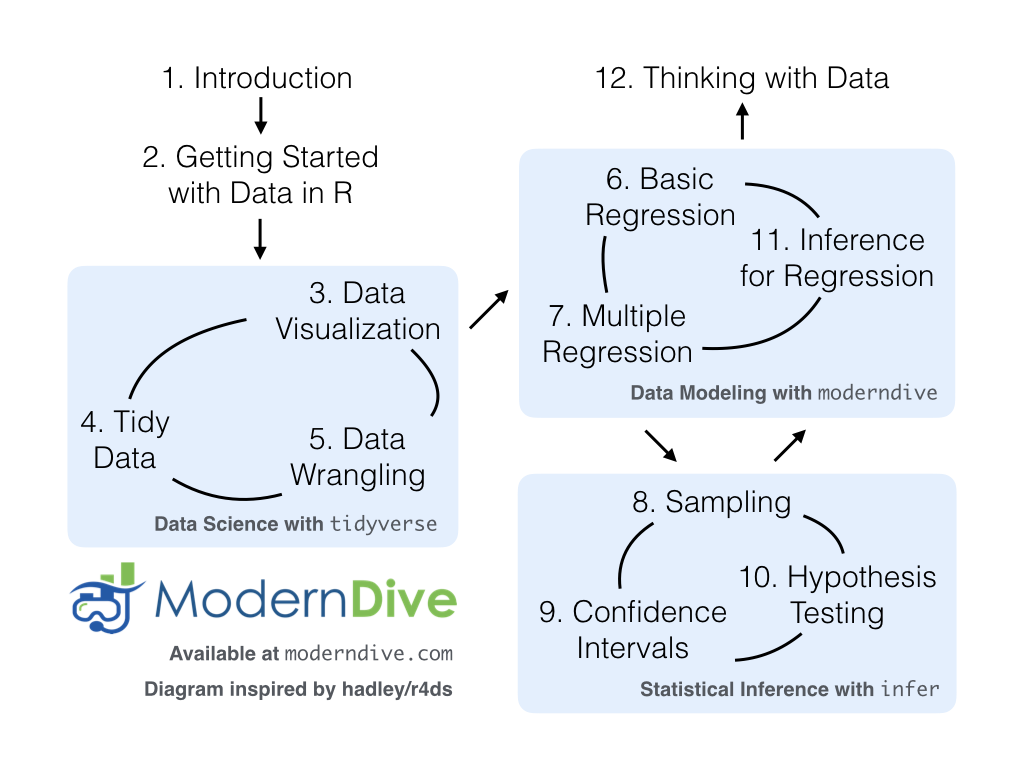
\includegraphics[width=\textwidth]{images/flowcharts/flowchart/flowchart.002} 

}

\caption{ModernDive Flowchart}\label{fig:moderndive-figure}
\end{figure}

\subsection{What you will learn from this
book}\label{subsec:learning-goals}

We hope that by the end of this book, you'll have learned

\begin{enumerate}
\def\labelenumi{\arabic{enumi}.}
\tightlist
\item
  How to use R to explore data.\\
\item
  How to answer statistical questions using tools like confidence
  intervals and hypothesis tests.
\item
  How to effectively create ``data stories'' using these tools.
\end{enumerate}

What do we mean by data stories? We mean any analysis involving data
that engages the reader in answering questions with careful visuals and
thoughtful discussion, such as
\href{http://rpubs.com/ry_lisa_elana/chicago}{How strong is the
relationship between per capita income and crime in Chicago
neighborhoods?} and
\href{https://ismayc.github.io/soc301_s2017/group_projects/group4.html}{How
many f**ks does Quentin Tarantino give (as measured by the amount of
swearing in his films)?}. Further discussions on data stories can be
found in this
\href{https://www.thinkwithgoogle.com/marketing-resources/data-measurement/tell-meaningful-stories-with-data/}{Think
With Google article}.

For other examples of data stories constructed by students like
yourselves, look at the final projects for two courses that have
previously used ModernDive:

\begin{itemize}
\tightlist
\item
  Middlebury College
  \href{https://rudeboybert.github.io/MATH116/PS/final_project/final_project_outline.html\#past_examples}{MATH
  116 Introduction to Statistical and Data Sciences} using student
  collected data.
\item
  Pacific University
  \href{https://ismayc.github.io/soc301_s2017/group-projects/index.html}{SOC
  301 Social Statistics} using data from the
  \href{https://cran.r-project.org/web/packages/fivethirtyeight/vignettes/fivethirtyeight.html}{fivethirtyeight
  R package}.
\end{itemize}

This book will help you develop your ``data science toolbox'', including
tools such as data visualization, data formatting, data wrangling, and
data modeling using regression. With these tools, you'll be able to
perform the entirety of the ``data/science pipeline'' while building
data communication skills (see Subsection \ref{subsec:pipeline} for more
details).

In particular, this book will lean heavily on data visualization. In
today's world, we are bombarded with graphics that attempt to convey
ideas. We will explore what makes a good graphic and what the standard
ways are to convey relationships with data. You'll also see the use of
visualization to introduce concepts like mean, median, standard
deviation, distributions, etc. In general, we'll use visualization as a
way of building almost all of the ideas in this book.

To impart the statistical lessons in this book, we have intentionally
minimized the number of mathematical formulas used and instead have
focused on developing a conceptual understanding via data visualization,
statistical computing, and simulations. We hope this is a more intuitive
experience than the way statistics has traditionally been taught in the
past and how it is commonly perceived.

Finally, you'll learn the importance of literate programming. By this we
mean you'll learn how to write code that is useful not just for a
computer to execute but also for readers to understand exactly what your
analysis is doing and how you did it. This is part of a greater effort
to encourage reproducible research (see Subsection
\ref{subsec:reproducible} for more details). Hal Abelson coined the
phrase that we will follow throughout this book:

\begin{quote}
``Programs must be written for people to read, and only incidentally for
machines to execute.''
\end{quote}

We understand that there may be challenging moments as you learn to
program. Both of us continue to struggle and find ourselves often using
web searches to find answers and reach out to colleagues for help. In
the long run though, we all can solve problems faster and more elegantly
via programming. We wrote this book as our way to help you get started
and you should know that there is a huge community of R users that are
always happy to help everyone along as well. This community exists in
particular on the internet on various forums and websites such as
\href{https://stackoverflow.com/}{stackoverflow.com}.

\subsection{Data/science pipeline}\label{subsec:pipeline}

You may think of statistics as just being a bunch of numbers. We
commonly hear the phrase ``statistician'' when listening to broadcasts
of sporting events. Statistics (in particular, data analysis), in
addition to describing numbers like with baseball batting averages,
plays a vital role in all of the sciences. You'll commonly hear the
phrase ``statistically significant'' thrown around in the media. You'll
see articles that say ``Science now shows that chocolate is good for
you.'' Underpinning these claims is data analysis. By the end of this
book, you'll be able to better understand whether these claims should be
trusted or whether we should be wary. Inside data analysis are many
sub-fields that we will discuss throughout this book (though not
necessarily in this order):

\begin{itemize}
\tightlist
\item
  data collection
\item
  data wrangling
\item
  data visualization
\item
  data modeling
\item
  inference
\item
  correlation and regression
\item
  interpretation of results
\item
  data communication/storytelling
\end{itemize}

These sub-fields are summarized in what Grolemund and Wickham term the
\href{http://r4ds.had.co.nz/explore-intro.html}{``Data/Science
Pipeline''} in Figure \ref{fig:pipeline-figure}.

\begin{figure}

{\centering 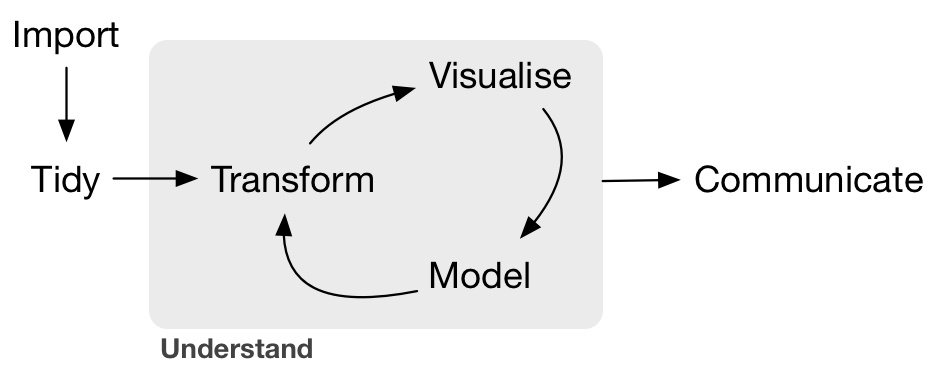
\includegraphics[width=\textwidth]{images/tidy1} 

}

\caption{Data/Science Pipeline}\label{fig:pipeline-figure}
\end{figure}

We will begin by digging into the gray \textbf{Understand} portion of
the cycle with data visualization, then with a discussion on what is
meant by tidy data and data wrangling, and then conclude by talking
about interpreting and discussing the results of our models via
\textbf{Communication}. These steps are vital to any statistical
analysis. But why should you care about statistics? ``Why did they make
me take this class?''

There's a reason so many fields require a statistics course. Scientific
knowledge grows through an understanding of statistical significance and
data analysis. You needn't be intimidated by statistics. It's not the
beast that it used to be and, paired with computation, you'll see how
reproducible research in the sciences particularly increases scientific
knowledge.

\subsection{Reproducible research}\label{subsec:reproducible}

\begin{quote}
``The most important tool is the \emph{mindset}, when starting, that the
end product will be reproducible.'' -- Keith Baggerly
\end{quote}

Another goal of this book is to help readers understand the importance
of reproducible analyses. The hope is to get readers into the habit of
making their analyses reproducible from the very beginning. This means
we'll be trying to help you build new habits. This will take practice
and be difficult at times. You'll see just why it is so important for
you to keep track of your code and well-document it to help yourself
later and any potential collaborators as well.

Copying and pasting results from one program into a word processor is
not the way that efficient and effective scientific research is
conducted. It's much more important for time to be spent on data
collection and data analysis and not on copying and pasting plots back
and forth across a variety of programs.

In a traditional analyses if an error was made with the original data,
we'd need to step through the entire process again: recreate the plots
and copy and paste all of the new plots and our statistical analysis
into your document. This is error prone and a frustrating use of time.
We'll see how to use R Markdown to get away from this tedious activity
so that we can spend more time doing science.

\begin{quote}
``We are talking about \emph{computational} reproducibility.'' - Yihui
Xie
\end{quote}

Reproducibility means a lot of things in terms of different scientific
fields. Are experiments conducted in a way that another researcher could
follow the steps and get similar results? In this book, we will focus on
what is known as \textbf{computational reproducibility}. This refers to
being able to pass all of one's data analysis, data-sets, and
conclusions to someone else and have them get exactly the same results
on their machine. This allows for time to be spent interpreting results
and considering assumptions instead of the more error prone way of
starting from scratch or following a list of steps that may be different
from machine to machine.

\subsection{Final note for students}\label{final-note-for-students}

At this point, if you are interested in instructor perspectives on this
book, ways to contribute and collaborate, or the technical details of
this book's construction and publishing, then continue with the rest of
the chapter below. Otherwise, let's get started with R and RStudio in
Chapter \ref{getting-started}!

\begin{center}\rule{0.5\linewidth}{\linethickness}\end{center}

\hypertarget{sec:intro-instructors}{\section{Introduction for
instructors}\label{sec:intro-instructors}}

This book is inspired by the following books:

\begin{itemize}
\tightlist
\item
  ``Mathematical Statistics with Resampling and R'' \citep{hester2011},
\item
  ``OpenIntro: Intro Stat with Randomization and Simulation''
  \citep{isrs2014}, and
\item
  ``R for Data Science'' \citep{rds2016}.
\end{itemize}

The first book, while designed for upper-level undergraduates and
graduate students, provides an excellent resource on how to use
resampling to impart statistical concepts like sampling distributions
using computation instead of large-sample approximations and other
mathematical formulas. The last two books are free options to learning
introductory statistics and data science, providing an alternative to
the many traditionally expensive introductory statistics textbooks.

When looking over the large number of introductory statistics textbooks
that currently exist, we found that there wasn't one that incorporated
many newly developed R packages directly into the text, in particular
the many packages included in the
\href{http://tidyverse.org/}{\texttt{tidyverse}} collection of packages,
such as \texttt{ggplot2}, \texttt{dplyr}, \texttt{tidyr}, and
\texttt{broom}. Additionally, there wasn't an open-source and easily
reproducible textbook available that exposed new learners all of three
of the learning goals listed at the outset of Subsection
\ref{subsec:learning-goals}.

\subsection{Who is this book for?}\label{who-is-this-book-for}

This book is intended for instructors of traditional introductory
statistics classes using RStudio, either the desktop or server version,
who would like to inject more data science topics into their syllabus.
We assume that students taking the class will have no prior algebra,
calculus, nor programming/coding experience.

Here are some principles and beliefs we kept in mind while writing this
text. If you agree with them, this might be the book for you.

\begin{enumerate}
\def\labelenumi{\arabic{enumi}.}
\tightlist
\item
  \textbf{Blur the lines between lecture and lab}

  \begin{itemize}
  \tightlist
  \item
    With increased availability and accessibility of laptops and
    open-source non-proprietary statistical software, the strict
    dichotomy between lab and lecture can be loosened.
  \item
    It's much harder for students to understand the importance of using
    software if they only use it once a week or less. They forget the
    syntax in much the same way someone learning a foreign language
    forgets the rules. Frequent reinforcement is key.
  \end{itemize}
\item
  \textbf{Focus on the entire data/science research pipeline}

  \begin{itemize}
  \tightlist
  \item
    We believe that the entirety of Grolemund and Wickham's
    \href{http://r4ds.had.co.nz/introduction.html}{data/science
    pipeline} should be taught.
  \item
    We believe in \href{https://arxiv.org/abs/1507.05346}{``minimizing
    prerequisites to research''}: students should be answering questions
    with data as soon as possible.
  \end{itemize}
\item
  \textbf{It's all about the data}

  \begin{itemize}
  \tightlist
  \item
    We leverage R packages for rich, real, and realistic data-sets that
    at the same time are easy-to-load into R, such as the
    \texttt{nycflights13} and \texttt{fivethirtyeight} packages.
  \item
    We believe that \href{http://escholarship.org/uc/item/84v3774z}{data
    visualization is a gateway drug for statistics} and that the Grammar
    of Graphics as implemented in the \texttt{ggplot2} package is the
    best way to impart such lessons. However, we often hear: ``You can't
    teach \texttt{ggplot2} for data visualization in intro stats!'' We,
    like
    \href{http://varianceexplained.org/r/teach_ggplot2_to_beginners/}{David
    Robinson}, are much more optimistic.
  \item
    \texttt{dplyr} has made data wrangling much more
    \href{http://chance.amstat.org/2015/04/setting-the-stage/}{accessible}
    to novices, and hence much more interesting data-sets can be
    explored.
  \end{itemize}
\item
  \textbf{Use simulation/resampling to introduce statistical inference,
  not probability/mathematical formulas}

  \begin{itemize}
  \tightlist
  \item
    Instead of using formulas, large-sample approximations, and
    probability tables, we teach statistical concepts using
    resampling-based inference.
  \item
    This allows for a de-emphasis of traditional probability topics,
    freeing up room in the syllabus for other topics.
  \end{itemize}
\item
  \textbf{Don't fence off students from the computation pool, throw them
  in!}

  \begin{itemize}
  \tightlist
  \item
    Computing skills are essential to working with data in the 21st
    century. Given this fact, we feel that to shield students from
    computing is to ultimately do them a disservice.
  \item
    We are not teaching a course on coding/programming per se, but
    rather just enough of the computational and algorithmic thinking
    necessary for data analysis.
  \end{itemize}
\item
  \textbf{Complete reproducibility and customizability}

  \begin{itemize}
  \tightlist
  \item
    We are frustrated when textbooks give examples, but not the source
    code and the data itself. We give you the source code for all
    examples as well as the whole book!
  \item
    Ultimately the best textbook is one you've written yourself. You
    know best your audience, their background, and their priorities. You
    know best your own style and the types of examples and problems you
    like best. Customization is the ultimate end. For more about how to
    make this book your own, see \protect\hyperlink{about-book}{About
    this Book}.
  \end{itemize}
\end{enumerate}

\begin{center}\rule{0.5\linewidth}{\linethickness}\end{center}

\section{DataCamp}\label{datacamp}

\begin{figure}
\centering

\includegraphics[width=1.00000\textwidth]{images/datacamp.png}
\caption{DataCamp logo}
\end{figure}

DataCamp is a browser-based interactive platform for learning data
science, offering courses on a wide array of courses on data science,
analytics, statistics, machine learning, and artificial intelligence,
where each course is a combination of lectures and exercises that offer
immediate feedback.

The following chapters of ModernDive roughly map to the following
closely-integrated DataCamp courses that use the same R tools and often
even the same datasets. By no means is this an exhaustive list of
possible DataCamp courses that are relevant to the topics in this book,
we recommend these ones in particular to supplement your ModernDive
experience.

Click on the image for each course to access its webpage on
\href{https://www.datacamp.com/home}{datacamp.com}. Instructors at
accredited universities can sign their class up for a free academic
licence at \href{https://www.datacamp.com/groups/education}{DataCamp For
The Classroom}, giving their students access to all premium courses for
6 months for free.

\begin{longtable}[]{@{}lll@{}}
\toprule
\begin{minipage}[b]{0.30\columnwidth}\raggedright\strut
Chapter\strut
\end{minipage} & \begin{minipage}[b]{0.30\columnwidth}\raggedright\strut
Topic\strut
\end{minipage} & \begin{minipage}[b]{0.30\columnwidth}\raggedright\strut
DataCamp Courses\strut
\end{minipage}\tabularnewline
\midrule
\endhead
\begin{minipage}[t]{0.30\columnwidth}\raggedright\strut
2\strut
\end{minipage} & \begin{minipage}[t]{0.30\columnwidth}\raggedright\strut
Basic R programming concepts\strut
\end{minipage} & \begin{minipage}[t]{0.30\columnwidth}\raggedright\strut
\href{https://www.datacamp.com/courses/free-introduction-to-r}{
\includegraphics[width=0.6\textwidth]{images/datacamp_intro_to_R.png}}
\href{https://www.datacamp.com/courses/intermediate-r}{
\includegraphics[width=0.6\textwidth]{images/datacamp_intermediate_R.png}}\strut
\end{minipage}\tabularnewline
\begin{minipage}[t]{0.30\columnwidth}\raggedright\strut
3 \& 5\strut
\end{minipage} & \begin{minipage}[t]{0.30\columnwidth}\raggedright\strut
Introductory data visualization and wrangling\strut
\end{minipage} & \begin{minipage}[t]{0.30\columnwidth}\raggedright\strut
\href{https://www.datacamp.com/courses/introduction-to-the-tidyverse}{
\includegraphics[width=0.6\textwidth]{images/datacamp_intro_to_tidyverse.png}}\strut
\end{minipage}\tabularnewline
\begin{minipage}[t]{0.30\columnwidth}\raggedright\strut
4 \& 5\strut
\end{minipage} & \begin{minipage}[t]{0.30\columnwidth}\raggedright\strut
Data ``tidying'' and intermediate data wrangling\strut
\end{minipage} & \begin{minipage}[t]{0.30\columnwidth}\raggedright\strut
\href{https://www.datacamp.com/courses/working-with-data-in-the-tidyverse}{
\includegraphics[width=0.6\textwidth]{images/datacamp_working_with_data.png}}\strut
\end{minipage}\tabularnewline
\begin{minipage}[t]{0.30\columnwidth}\raggedright\strut
6 \& 7\strut
\end{minipage} & \begin{minipage}[t]{0.30\columnwidth}\raggedright\strut
Data modeling, basic regression, and multiple regression\strut
\end{minipage} & \begin{minipage}[t]{0.30\columnwidth}\raggedright\strut
\href{https://www.datacamp.com/courses/modeling-with-data-in-the-tidyverse}{
\includegraphics[width=0.6\textwidth]{images/datacamp_intro_to_modeling.png}}\strut
\end{minipage}\tabularnewline
\begin{minipage}[t]{0.30\columnwidth}\raggedright\strut
9 \& 10\strut
\end{minipage} & \begin{minipage}[t]{0.30\columnwidth}\raggedright\strut
Statistical inference: confidence intervals and hypothesis testing\strut
\end{minipage} & \begin{minipage}[t]{0.30\columnwidth}\raggedright\strut
\href{https://www.datacamp.com/courses/inference-for-numerical-data}{
\includegraphics[width=0.6\textwidth]{images/datacamp_inference_for_numerical_data.png}}
\href{https://www.datacamp.com/courses/inference-for-categorical-data}{
\includegraphics[width=0.6\textwidth]{images/datacamp_inference_for_categorical_data.png}}\strut
\end{minipage}\tabularnewline
\begin{minipage}[t]{0.30\columnwidth}\raggedright\strut
11\strut
\end{minipage} & \begin{minipage}[t]{0.30\columnwidth}\raggedright\strut
Inference for regression\strut
\end{minipage} & \begin{minipage}[t]{0.30\columnwidth}\raggedright\strut
\href{https://www.datacamp.com/courses/inference-for-linear-regression}{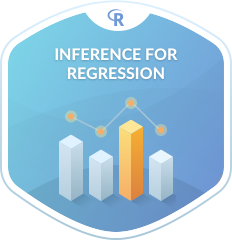
\includegraphics[width=0.6\textwidth]{images/datacamp_inference_for_regression.png}}\strut
\end{minipage}\tabularnewline
\bottomrule
\end{longtable}

\begin{center}\rule{0.5\linewidth}{\linethickness}\end{center}

\hypertarget{sec:connect-contribute}{\section{Connect and
contribute}\label{sec:connect-contribute}}

If you would like to connect with ModernDive, check out the following
links:

\begin{itemize}
\tightlist
\item
  If you would like to receive periodic updates about ModernDive
  (roughly every 3 months), please sign up for our
  \href{http://eepurl.com/cBkItf}{mailing list}.
\item
  Contact Albert at
  \href{mailto:albert.ys.kim@gmail.com}{\nolinkurl{albert.ys.kim@gmail.com}}
  and Chester at
  \href{mailto:chester.ismay@gmail.com}{\nolinkurl{chester.ismay@gmail.com}}.
\item
  We're on Twitter at \href{https://twitter.com/ModernDive}{ModernDive}.
\end{itemize}

If you would like to contribute to ModernDive, there are many ways!
Let's all work together to make this book as great as possible for as
many students and instructors as possible!

\begin{itemize}
\tightlist
\item
  Please let us know if you find any errors, typos, or areas from
  improvement on our
  \href{https://github.com/moderndive/moderndive_book/issues}{GitHub
  issues} page.
\item
  If you are familiar with GitHub and would like to contribute more,
  please see Section \ref{sec:about-book} below.
\end{itemize}

The authors would like to thank
\href{https://github.com/nsonneborn}{Nina Sonneborn},
\href{https://twitter.com/rhobott?lang=en}{Kristin Bott}, and the
participants of our
\href{https://www.causeweb.org/cause/uscots/uscots17/workshop/3}{USCOTS
2017 workshop} for their feedback and suggestions. A special thanks goes
to Dr.~Yana Weinstein, cognitive psychological scientist and co-founder
of \href{http://www.learningscientists.org/yana-weinstein/}{The Learning
Scientists}, for her extensive contributions.

\begin{center}\rule{0.5\linewidth}{\linethickness}\end{center}

\hypertarget{sec:about-book}{\section{About this
book}\label{sec:about-book}}

This book was written using RStudio's
\href{https://bookdown.org/}{bookdown} package by Yihui Xie
\citep{R-bookdown}. This package simplifies the publishing of books by
having all content written in
\href{http://rmarkdown.rstudio.com/html_document_format.html}{R
Markdown}. The bookdown/R Markdown source code for all versions of
ModernDive is available on GitHub:

\begin{itemize}
\tightlist
\item
  \textbf{Latest published version} The most up-to-date release:

  \begin{itemize}
  \tightlist
  \item
    Version 0.4.0 released on July 21, 2018
    (\href{https://github.com/moderndive/moderndive_book/releases/tag/v0.4.0}{source
    code}).
  \item
    Available at \href{https://moderndive.com/}{ModernDive.com}
  \end{itemize}
\item
  \textbf{Development version} The working copy of the next version
  which is currently being edited:

  \begin{itemize}
  \tightlist
  \item
    Preview of development version is available at
    \url{https://moderndive.netlify.com/}
  \item
    Source code: Available on ModernDive's
    \href{https://github.com/moderndive/moderndive_book}{GitHub
    repository page}
  \end{itemize}
\item
  \textbf{Previous versions} Older versions that may be out of date:

  \begin{itemize}
  \tightlist
  \item
    \href{previous_versions/v0.3.0/index.html}{Version 0.3.0} released
    on February 3, 2018
    (\href{https://github.com/moderndive/moderndive_book/releases/tag/v0.3.0}{source
    code})
  \item
    \href{previous_versions/v0.2.0/index.html}{Version 0.2.0} released
    on August 02, 2017
    (\href{https://github.com/moderndive/moderndive_book/releases/tag/v0.2.0}{source
    code})
  \item
    \href{previous_versions/v0.1.3/index.html}{Version 0.1.3} released
    on February 09, 2017
    (\href{https://github.com/moderndive/moderndive_book/releases/tag/v0.1.3}{source
    code})
  \item
    \href{previous_versions/v0.1.2/index.html}{Version 0.1.2} released
    on January 22, 2017
    (\href{https://github.com/moderndive/moderndive_book/releases/tag/v0.1.2}{source
    code})
  \end{itemize}
\end{itemize}

Could this be a new paradigm for textbooks? Instead of the traditional
model of textbook companies publishing updated \emph{editions} of the
textbook every few years, we apply a software design influenced model of
publishing more easily updated \emph{versions}. We can then leverage
open-source communities of instructors and developers for ideas, tools,
resources, and feedback. As such, we welcome your pull requests.

Finally, feel free to modify the book as you wish for your own needs,
but please list the authors at the top of \texttt{index.Rmd} as
``Chester Ismay, Albert Y. Kim, and YOU!''

\begin{center}\rule{0.5\linewidth}{\linethickness}\end{center}

\section{About the authors}\label{sec:about-authors}

Who we are!

\begin{longtable}[]{@{}cc@{}}
\toprule
Chester Ismay & Albert Y. Kim\tabularnewline
\midrule
\endhead
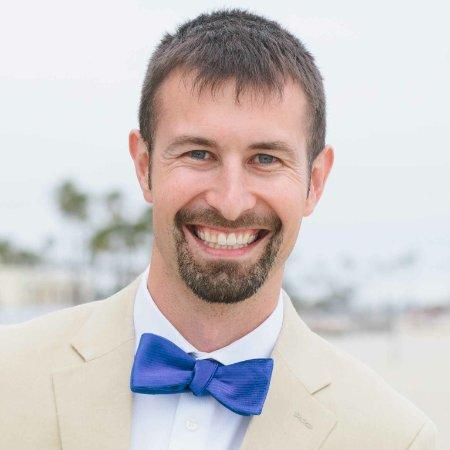
\includegraphics[width=0.40000\textwidth]{images/ismay.png} &
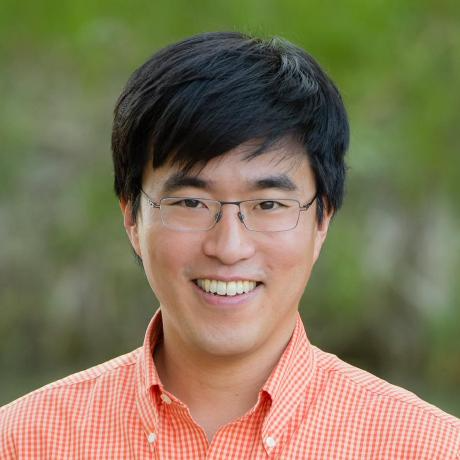
\includegraphics[width=0.40000\textwidth]{images/kim.png}\tabularnewline
\bottomrule
\end{longtable}

\begin{itemize}
\tightlist
\item
  Chester Ismay: Senior Curriculum Lead - DataCamp, Portland, OR, USA.

  \begin{itemize}
  \tightlist
  \item
    Email:
    \href{mailto:chester.ismay@gmail.com}{\nolinkurl{chester.ismay@gmail.com}}
  \item
    Webpage: \url{http://chester.rbind.io/}
  \item
    Twitter:
    \href{https://twitter.com/old_man_chester}{old\_man\_chester}
  \item
    GitHub: \url{https://github.com/ismayc}
  \end{itemize}
\item
  Albert Y. Kim: Assistant Professor of Statistical \& Data Sciences -
  Smith College, Northampton, MA, USA.

  \begin{itemize}
  \tightlist
  \item
    Email:
    \href{mailto:albert.ys.kim@gmail.com}{\nolinkurl{albert.ys.kim@gmail.com}}
  \item
    Webpage: \url{http://rudeboybert.rbind.io/}
  \item
    Twitter: \href{https://twitter.com/rudeboybert}{rudeboybert}
  \item
    GitHub: \url{https://github.com/rudeboybert}
  \end{itemize}
\end{itemize}

\chapter{Getting Started with Data in R}\label{getting-started}

Before we can start exploring data in R, there are some key concepts to
understand first:

\begin{enumerate}
\def\labelenumi{\arabic{enumi}.}
\tightlist
\item
  What are R and RStudio?
\item
  How do I code in R?
\item
  What are R packages?
\end{enumerate}

If you are already familiar with these concepts, feel free to skip to
Section \ref{nycflights13} below introducing some of the datasets we
will explore in depth in this book. Much of this chapter is based on two
sources which you should feel free to use as references if you are
looking for additional details:

\begin{enumerate}
\def\labelenumi{\arabic{enumi}.}
\tightlist
\item
  ModernDive co-author Chester Ismay's
  \href{http://ismayc.github.io/rbasics-book}{Getting used to R,
  RStudio, and R Markdown} \citep{usedtor2016} short book, which
  includes video screen recordings that you can follow along and pause
  as you learn.
\item
  DataCamp's online tutorials. DataCamp is a browser-based interactive
  platform for learning data science and their tutorials will help
  facilitate your learning of the above concepts (and other topics in
  this book). Go to \href{https://www.datacamp.com/}{DataCamp} and
  create an account before continuing.
\end{enumerate}

\begin{center}\rule{0.5\linewidth}{\linethickness}\end{center}

\section{What are R and RStudio?}\label{what-are-r-and-rstudio}

For much of this book, we will assume that you are using R via RStudio.
First time users often confuse the two. At its simplest:

\begin{itemize}
\tightlist
\item
  R is like a car's engine
\item
  RStudio is like a car's dashboard
\end{itemize}

\begin{longtable}[]{@{}cc@{}}
\toprule
R: Engine & RStudio: Dashboard\tabularnewline
\midrule
\endhead
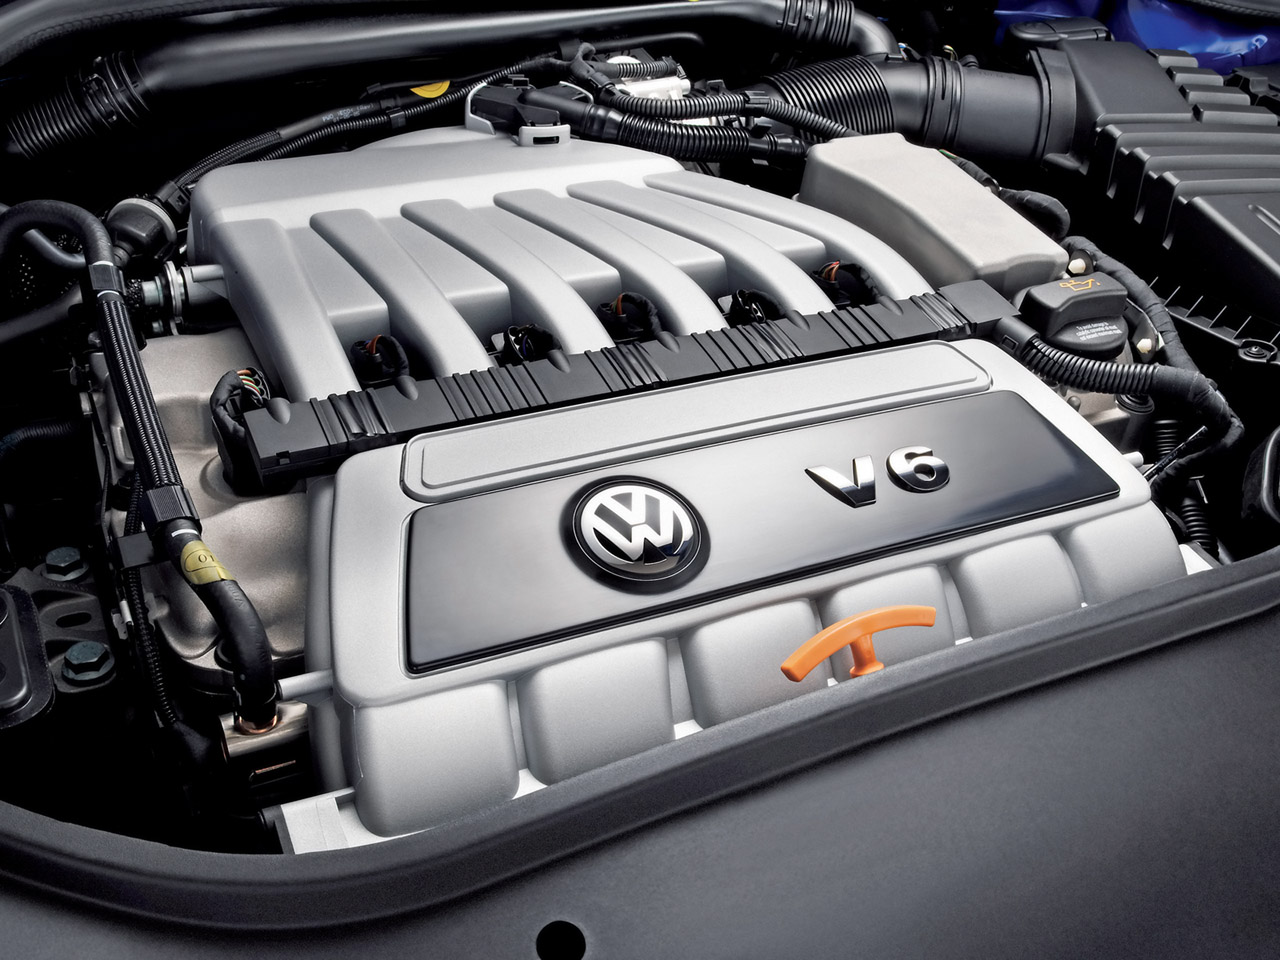
\includegraphics[height=1.70000in]{images/engine.jpg} &
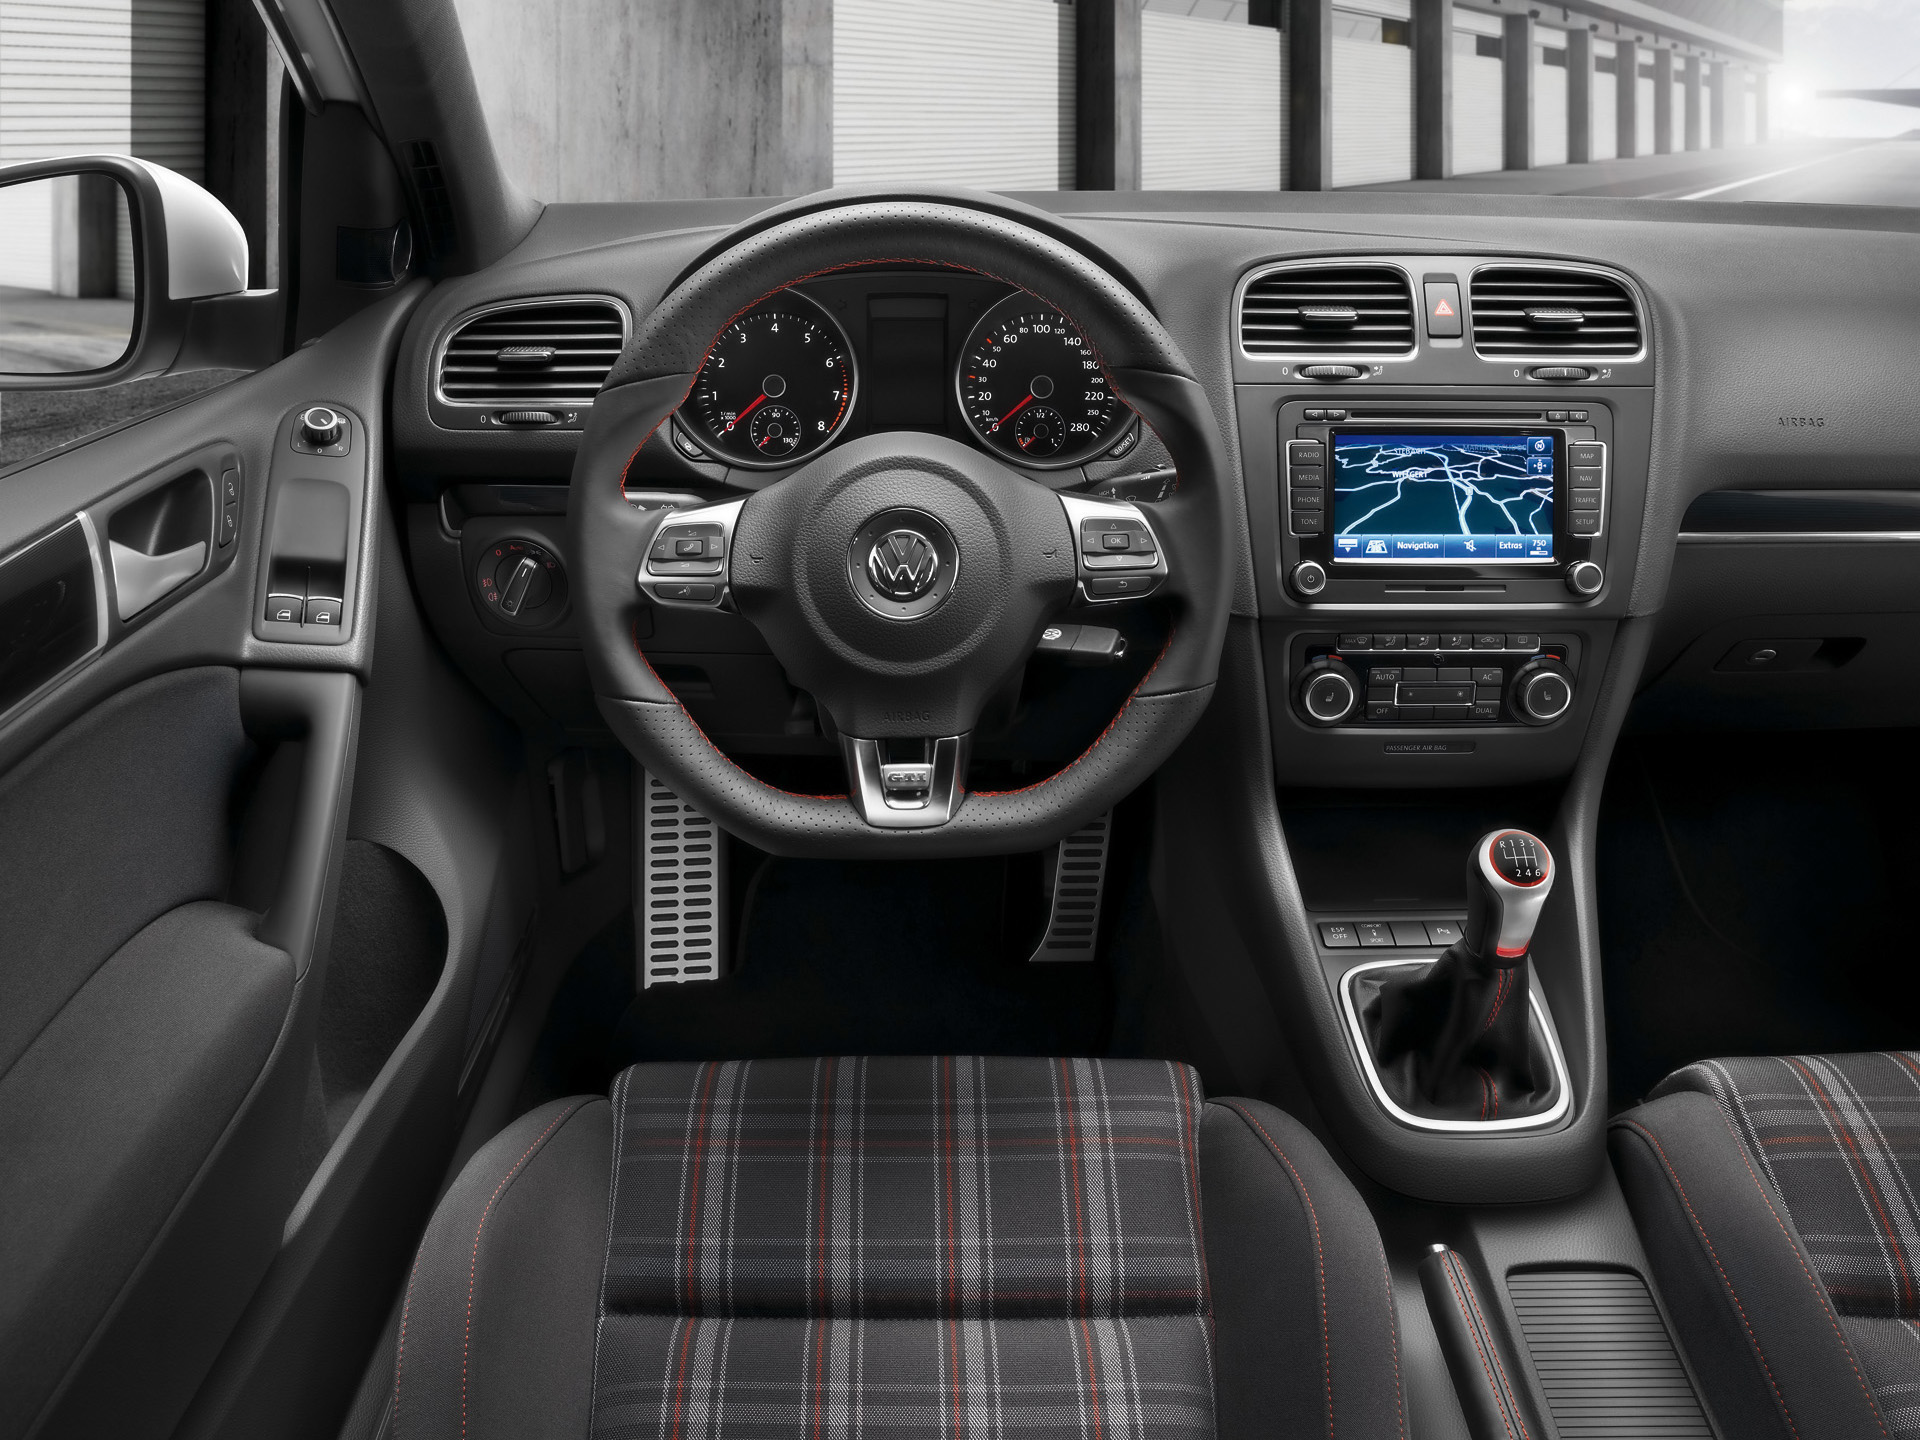
\includegraphics[height=1.70000in]{images/dashboard.jpg}\tabularnewline
\bottomrule
\end{longtable}

More precisely, R is a programming language that runs computations while
RStudio is an \emph{integrated development environment (IDE)} that
provides an interface by adding many convenient features and tools. So
the way of having access to a speedometer, rearview mirrors, and a
navigation system makes driving much easier, using RStudio's interface
makes using R much easier as well.

Optional: For a more in-depth discussion on the difference between R and
RStudio IDE, watch this
\href{https://campus.datacamp.com/courses/working-with-the-rstudio-ide-part-1/orientation?ex=1}{DataCamp
video (2m52s)}.

\subsection{Installing R and RStudio}\label{installing-r-and-rstudio}

\emph{If your instructor has provided you with a link and access to
RStudio Server, then you can skip this section. We do recommend though
after a few months of working on the RStudio Server that you return to
these instructions. If you don't know what RStudio Server is, then
please read this section.}

You will first need to download and install both R and RStudio (Desktop
version) on your computer.

\begin{enumerate}
\def\labelenumi{\arabic{enumi}.}
\tightlist
\item
  \href{https://cran.r-project.org/}{Download and install R}.

  \begin{itemize}
  \tightlist
  \item
    Note: You must do this first.
  \item
    Click on the download link corresponding to your computer's
    operating system.
  \end{itemize}
\item
  \href{https://www.rstudio.com/products/rstudio/download3/}{Download
  and install RStudio}.

  \begin{itemize}
  \tightlist
  \item
    Scroll down to ``Installers for Supported Platforms''
  \item
    Click on the download link corresponding to your computer's
    operating system.
  \end{itemize}
\end{enumerate}

Optional: If you need more detailed instructions on how to install R and
RStudio, watch this
\href{https://campus.datacamp.com/courses/working-with-the-rstudio-ide-part-1/orientation?ex=3}{DataCamp
video (1m22s)}.

\subsection{Using R via RStudio}\label{using-r-via-rstudio}

Recall our car analogy from above. Much as we don't drive a car by
interacting directly with the engine but rather by using elements on the
car's dashboard, we won't be using R directly but rather we will use
RStudio's interface. After you install R and RStudio on your computer,
you'll have two new programs AKA applications you can open. We will
always work in RStudio and not R. In other words:

\begin{longtable}[]{@{}cc@{}}
\toprule
R: Do not open this & RStudio: Open this\tabularnewline
\midrule
\endhead

\includegraphics[width=0.25000\textwidth]{images/Rlogo.png} &

\includegraphics[width=0.20000\textwidth]{images/RStudio-Ball.png}\tabularnewline
\bottomrule
\end{longtable}

After you open RStudio, you should see the following:

\begin{figure}
\centering
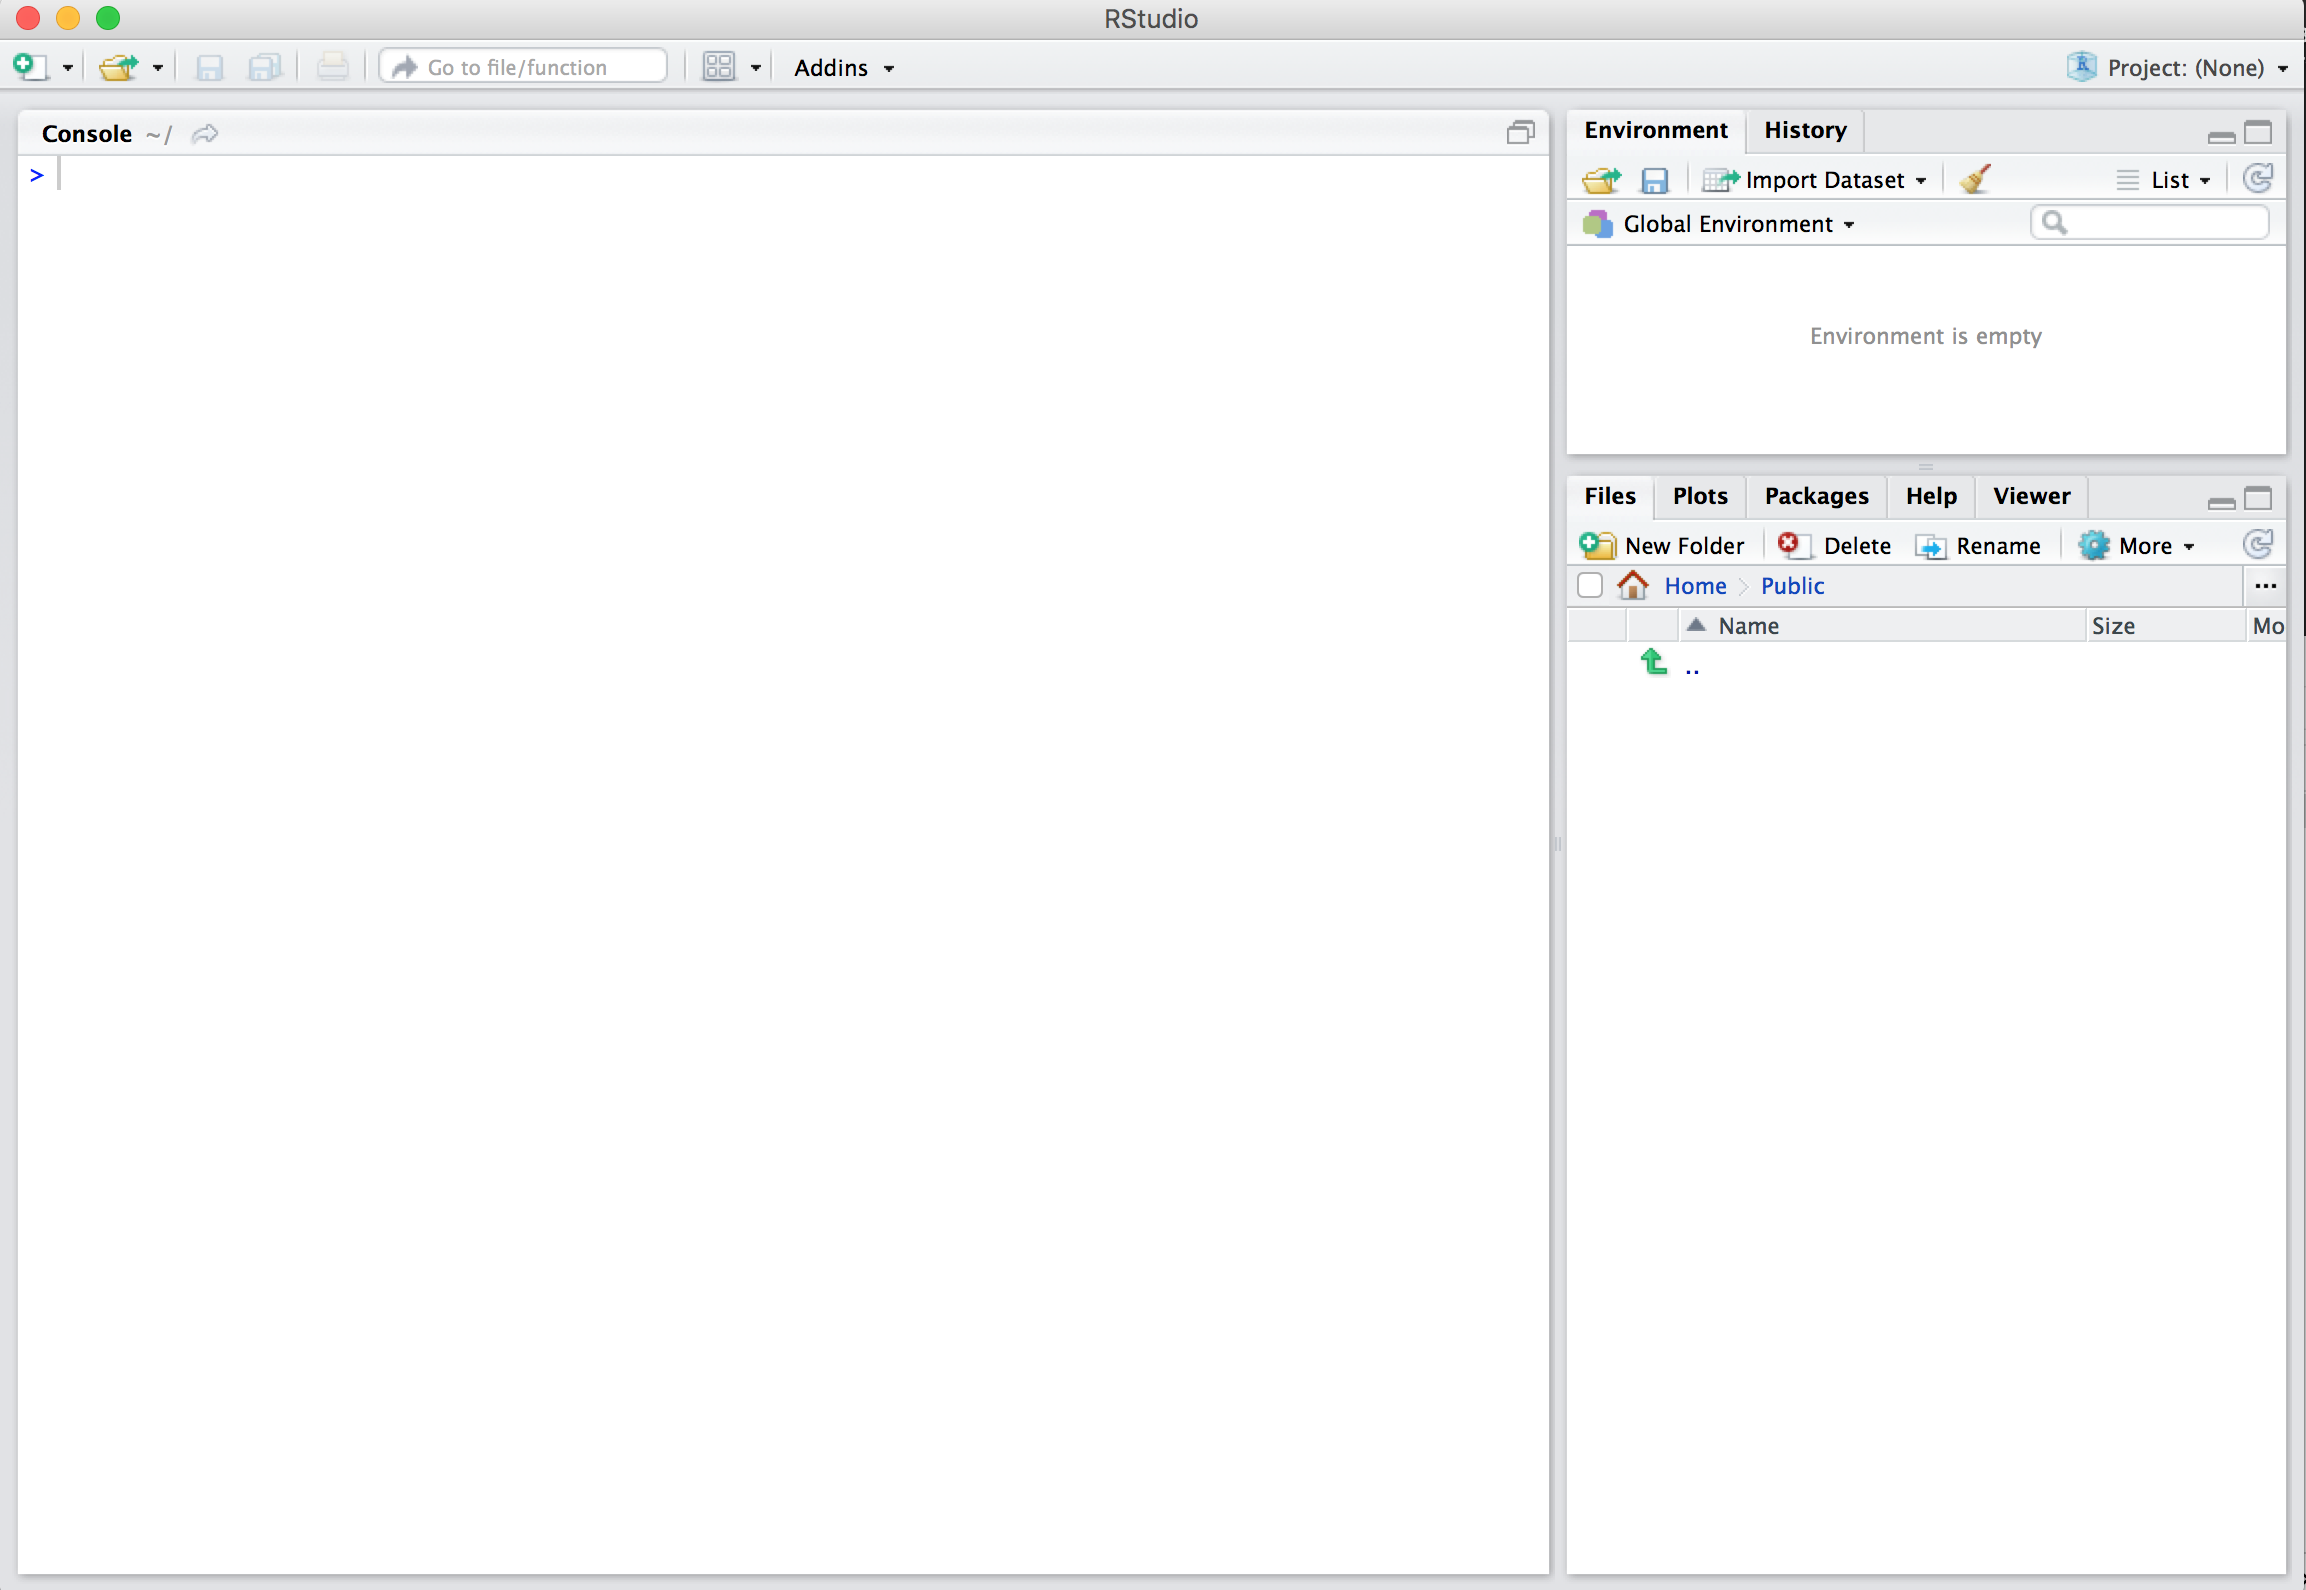
\includegraphics{images/rstudio.png}
\caption{RStudio}
\end{figure}

Watch the following
\href{https://campus.datacamp.com/courses/working-with-the-rstudio-ide-part-1/orientation?ex=5}{DataCamp
video (4m10s)} to learn about the different \emph{panes} in RStudio, in
particular the \emph{Console pane} where you will later run R code.

\begin{center}\rule{0.5\linewidth}{\linethickness}\end{center}

\section{How do I code in R?}\label{code}

Now that you're set up with R and RStudio, you are probably asking
yourself ``OK. Now how do I use R?'' The first thing to note as that
unlike other software like Excel, STATA, or SAS that provide
\href{https://en.wikipedia.org/wiki/Point_and_click}{point and click}
interfaces, R is an
\href{https://en.wikipedia.org/wiki/Interpreted_language}{interpreted
language}, meaning you have to enter in R commands written in R code
i.e.~you have to program in R (we use the terms ``coding'' and
``programming'' interchangeably in this book).

While it is not required to be a seasoned coder/computer programmer to
use R, there is still a set of basic programming concepts that R users
need to understand. Consequently, while this book is not a book on
programming, you will still learn just enough of these basic programming
concepts needed to explore and analyze data effectively.

\subsection{Basic programming concepts and
terminology}\label{programming-concepts}

To introduce you to many of these basic programming concepts and
terminology, we direct you to the following DataCamp online interactive
tutorials. For each of the tutorials, we give a list of the basic
programming concepts covered. Note that in this book, we will use a
different font to distinguish regular font from \texttt{computer\_code}.

It is important to note that while these tutorials serve as excellent
introductions, a single pass through them is insufficient for long-term
learning and retention. The ultimate tools for long-term learning and
retention are ``learning by doing'' and repetition, something we will
have you do over the course of the entire book and we encourage this
process as much as possible as you learn any new skill.

\begin{itemize}
\tightlist
\item
  From the
  \href{https://www.datacamp.com/courses/free-introduction-to-r}{Introduction
  to R} course complete the following chapters. As you work through the
  chapters, carefully note the important terms and what they are used
  for. We recommend you do so in a notebook that you can easily refer
  back to.

  \begin{itemize}
  \tightlist
  \item
    \href{https://campus.datacamp.com/courses/free-introduction-to-r/chapter-1-intro-to-basics-1?ex=1}{Chapter
    1 Intro to basics}:

    \begin{itemize}
    \tightlist
    \item
      Console pane: where you enter in commands
    \item
      Objects: where values are saved, how to assign values to objects.
    \item
      Data types: integers, doubles/numerics, logicals, characters.\\
    \end{itemize}
  \item
    \href{https://campus.datacamp.com/courses/free-introduction-to-r/chapter-2-vectors-2?ex=1}{Chapter
    2 Vectors}:

    \begin{itemize}
    \tightlist
    \item
      Vectors: a series of values.
    \end{itemize}
  \item
    \href{https://campus.datacamp.com/courses/free-introduction-to-r/chapter-4-factors-4?ex=1}{Chapter
    4 Factors}:

    \begin{itemize}
    \tightlist
    \item
      \emph{Categorical data} (as opposed to \emph{numerical data}) are
      represented in R as \texttt{factor}s.
    \end{itemize}
  \item
    \href{https://campus.datacamp.com/courses/free-introduction-to-r/chapter-5-data-frames?ex=1}{Chapter
    5 Data frames}:

    \begin{itemize}
    \tightlist
    \item
      Data frames are analogous to rectangular spreadsheets: they are
      representations of datasets in R where the rows correspond
      \emph{observations} and the columns correspond to \emph{variables}
      that describe the observations. We will revisit this later in
      Section \ref{nycflights13}.
    \end{itemize}
  \end{itemize}
\item
  From the
  \href{https://www.datacamp.com/courses/intermediate-r}{Intermediate R}
  course complete the following chapters:

  \begin{itemize}
  \tightlist
  \item
    \href{https://campus.datacamp.com/courses/intermediate-r/chapter-1-conditionals-and-control-flow?ex=1}{Chapter
    1 Conditionals and Control Flow}:

    \begin{itemize}
    \tightlist
    \item
      Testing for equality in R using \texttt{==} (and not \texttt{=}
      which is typically used for assignment). Ex:
      \texttt{2\ +\ 1\ ==\ 3} compares \texttt{2\ +\ 1} to \texttt{3}
      and is correct R syntax, while \texttt{2\ +\ 1\ =\ 3} is not and
      is incorrect R syntax.
    \item
      Boolean algebra: \texttt{TRUE/FALSE} statements and mathematical
      operators such as \texttt{\textless{}} (less than),
      \texttt{\textless{}=} (less than or equal), and \texttt{!=} (not
      equal to).
    \item
      Logical operators: \texttt{\&} representing ``and'',
      \texttt{\textbar{}} representing ``or''. Ex:
      \texttt{(2\ +\ 1\ ==\ 3)\ \&\ (2\ +\ 1\ ==\ 4)} returns
      \texttt{FALSE} while
      \texttt{(2\ +\ 1\ ==\ 3)\ \textbar{}\ (2\ +\ 1\ ==\ 4)} returns
      \texttt{TRUE}.
    \end{itemize}
  \item
    \href{https://campus.datacamp.com/courses/intermediate-r/chapter-3-functions?ex=1}{Chapter
    3 Functions}:

    \begin{itemize}
    \tightlist
    \item
      Concept of functions: they take in inputs (called
      \emph{arguments}) and return outputs.
    \item
      You either manually specify a function's arguments or use the
      function's \emph{defaults}.
    \end{itemize}
  \end{itemize}
\end{itemize}

This list is by no means an exhaustive list of all the programming
concepts and terminology needed to become a savvy R user; such a list
would be so large it wouldn't be very useful, especially for novices.
Rather, we feel this is the bare minimum you need to know before you get
started; the rest we feel you can learn as you go. Remember that your
knowledge of all of these concepts will build as you get better and
better at ``speaking R'' and getting used to its syntax.

\subsection{Tips on learning to code}\label{tips-on-learning-to-code}

Learning to code/program is very much like learning a foreign language,
it can be very daunting and frustrating at first. However just as with
learning a foreign language, if you put in the effort and are not afraid
to make mistakes, anybody can learn. Lastly, there are a few useful
things to keep in mind as you learn to program:

\begin{itemize}
\tightlist
\item
  \textbf{Computers are stupid}: You have to tell a computer everything
  it needs to do. Furthermore, your instructions can't have any mistakes
  in them, nor can they be ambiguous in any way.
\item
  \textbf{Take the ``copy/paste/tweak'' approach}: Especially when
  learning your first programming language, it is often much easier to
  taking existing code that you know works and modify it to suit your
  ends, rather than trying to write new code from scratch. We call this
  the \emph{copy/paste/tweak} approach. So early on, we suggest not
  trying to code from scratch, but please take the code we provide
  throughout this book and play around with it!
\item
  \textbf{Practice is key}: Just as the only solution to improving your
  foreign language skills is practice, so also the only way to get
  better at R is through practice. Don't worry however, we'll give you
  plenty of opportunities to practice!
\end{itemize}

\begin{center}\rule{0.5\linewidth}{\linethickness}\end{center}

\section{What are R packages?}\label{packages}

Another point of confusion with new R users is the notion of a package.
R packages extend the functionality of R by providing additional
functions, data, and documentation and can be downloaded for free from
the internet. They are written by a world-wide community of R users. For
example, among the many packages we will use in this book are the

\begin{itemize}
\tightlist
\item
  \texttt{ggplot2} package for data visualization in Chapter \ref{viz}
\item
  \texttt{dplyr} package for data wrangling in Chapter \ref{wrangling}
\end{itemize}

There are two key things to remember about R packages:

\begin{enumerate}
\def\labelenumi{\arabic{enumi}.}
\tightlist
\item
  \emph{Installation}: Most packages are not installed by default when
  you install R and RStudio. You need to install a package before you
  can use it. Once you've installed it, you likely don't need to install
  it again unless you want to update it to a newer version of the
  package.
\item
  \emph{Loading}: Packages are not loaded automatically when you open
  RStudio. You need to load them every time you open RStudio using the
  \texttt{library()} command.
\end{enumerate}

A good analogy for R packages is they are like apps you can download
onto a mobile phone:

\begin{longtable}[]{@{}cc@{}}
\toprule
R: A new phone & R Packages: Apps you can download\tabularnewline
\midrule
\endhead
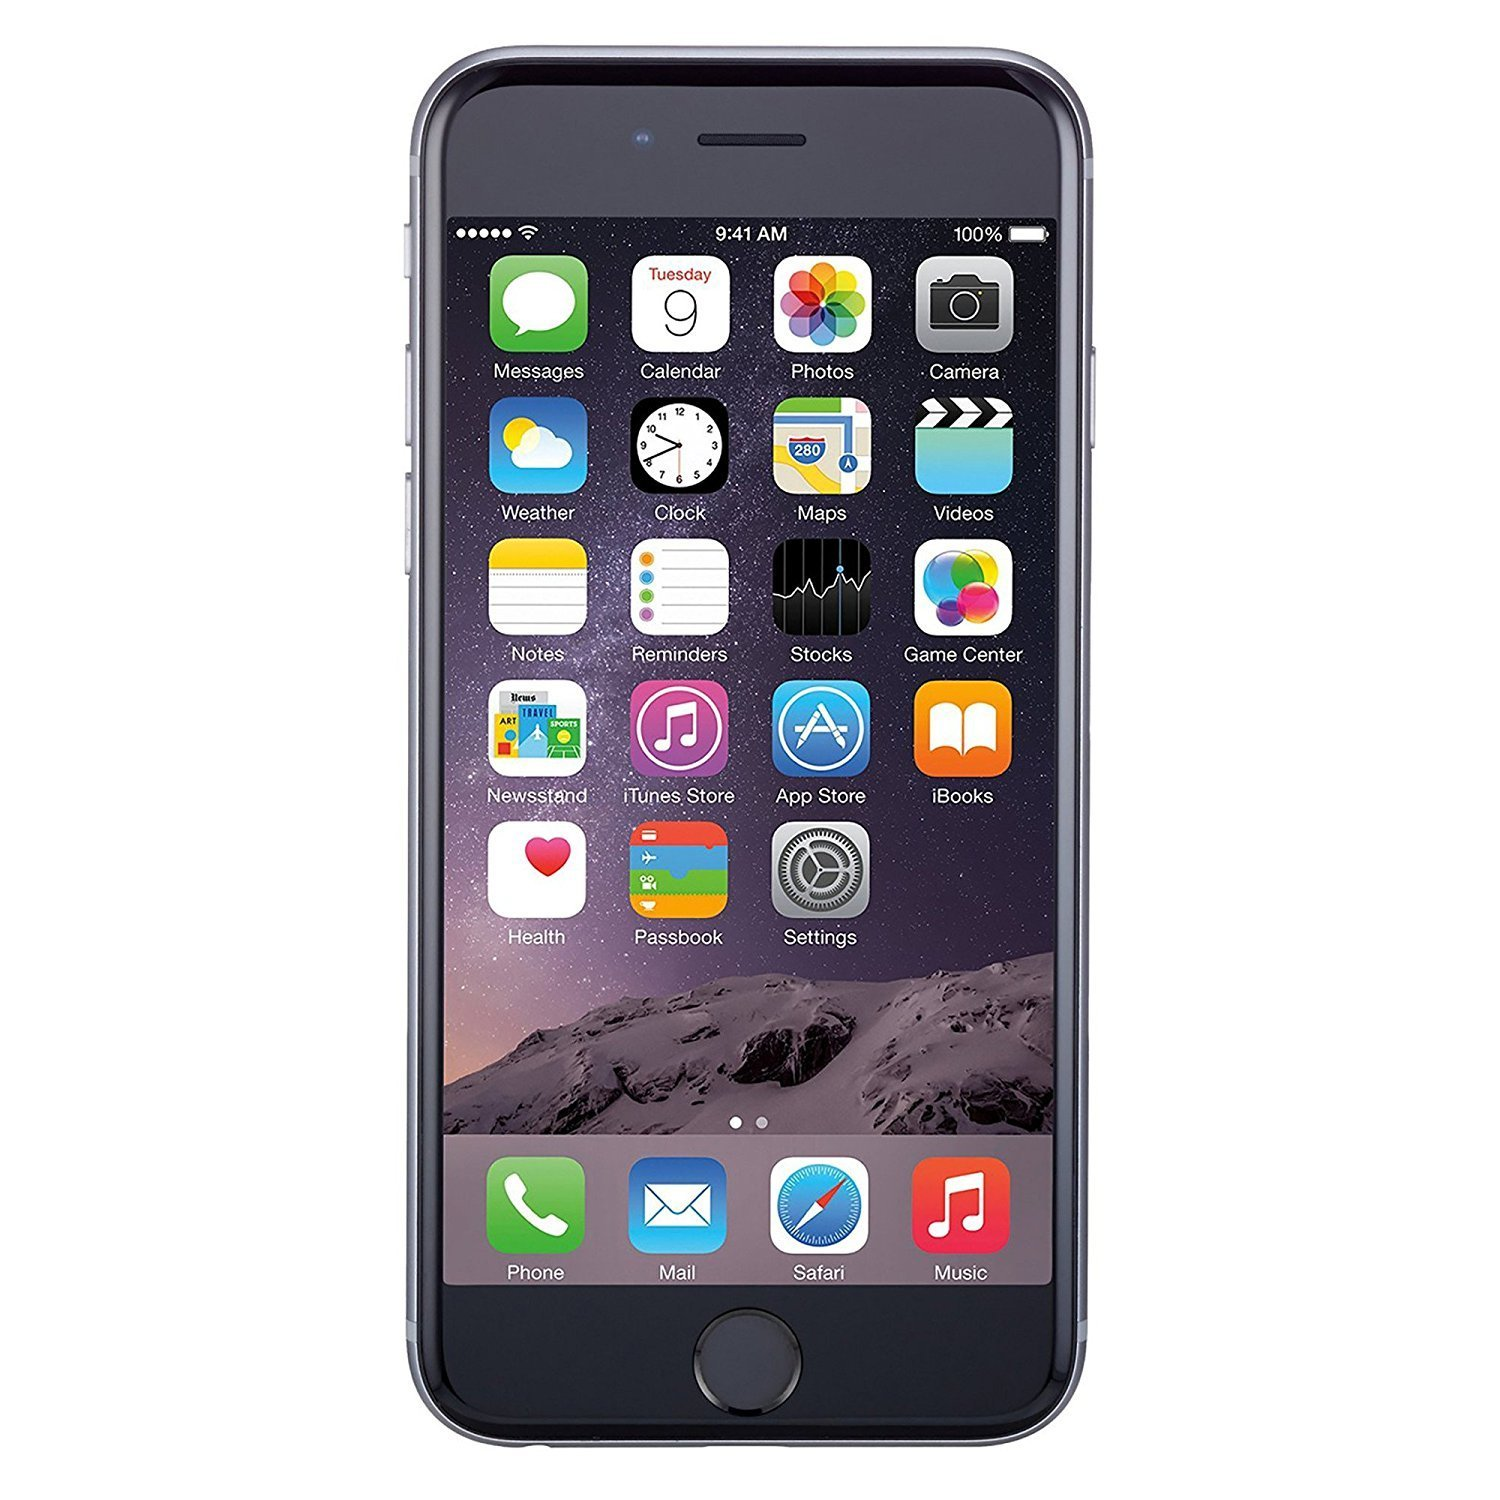
\includegraphics[height=1.50000in]{images/iphone.jpg} &

\includegraphics[height=1.50000in]{images/apps.jpg}\tabularnewline
\bottomrule
\end{longtable}

So, expanding on this analogy a bit:

\begin{enumerate}
\def\labelenumi{\arabic{enumi}.}
\tightlist
\item
  R is like a new mobile phone. It has a certain amount of functionality
  when you use it for the first time, but it doesn't have everything.
\item
  R packages are like the apps you can download onto your phone, much
  like those offered in the App Store and Google Play. For example:
  Instagram.
\item
  In order to use a package, just like in order to use Instagram, you
  must:

  \begin{enumerate}
  \def\labelenumii{\arabic{enumii}.}
  \tightlist
  \item
    First download it and install it. You do this only once.
  \item
    Load it, or in other words, ``open'' it, using the
    \texttt{library()} command.
  \end{enumerate}
\end{enumerate}

So just as you can only start sharing photos with your friends on
Instagram if you first install the app and then open it, you can only
access an R package's data and functions if you first install the
package and then load it with the \texttt{library()} command. Let's
cover these two steps:

\subsection{Package installation}\label{package-installation}

(Note that if you are working on an RStudio Server, you probably will
not need to install your own packages as that has been already done for
you. Still it is important that you know this process for later when you
are not using the RStudio Server but rather your own installation of
RStudio Desktop.)

There are two ways to install an R package. For example, to install the
\texttt{ggplot2} package:

\begin{enumerate}
\def\labelenumi{\arabic{enumi}.}
\tightlist
\item
  \textbf{Easy way}: In the Files pane of RStudio:

  \begin{enumerate}
  \def\labelenumii{\alph{enumii})}
  \tightlist
  \item
    Click on the ``Packages'' tab
  \item
    Click on ``Install''
  \item
    Type the name of the package under ``Packages (separate multiple
    with space or comma):'' In this case, type \texttt{ggplot2}
  \item
    Click ``Install''
  \end{enumerate}
\item
  \textbf{Alternative way}: In the Console pane run
  \texttt{install.packages("ggplot2")} (you must include the quotation
  marks).
\end{enumerate}

Repeat this for the \texttt{dplyr} and \texttt{nycflights13} packages.

\textbf{Note}: You only have to install a package once, unless you want
to update an already installed package to the latest version. If you
want to update a package to the latest version, then re-install it by
repeating the above steps.

\subsection{Package loading}\label{package-loading}

After you've installed a package, you can now load it using the
\texttt{library()} command. For example, to load the \texttt{ggplot2}
and \texttt{dplyr} packages, run the following code in the Console pane:

\begin{Shaded}
\begin{Highlighting}[]
\KeywordTok{library}\NormalTok{(ggplot2)}
\KeywordTok{library}\NormalTok{(dplyr)}
\end{Highlighting}
\end{Shaded}

\textbf{Note}: You have to reload each package you want to use every
time you open a new session of RStudio. This is a little annoying to get
used to and will be your most common error as you begin. When you see an
error such as

\begin{verbatim}
Error: could not find function
\end{verbatim}

remember that this likely comes from you trying to use a function in a
package that has not been loaded. Remember to run the \texttt{library()}
function with the appropriate package to fix this error.

\begin{center}\rule{0.5\linewidth}{\linethickness}\end{center}

\section{Explore your first dataset}\label{nycflights13}

Let's put everything we've learned so far into practice and start
exploring some real data! Data comes to us in a variety of formats, from
pictures to text to numbers. Throughout this book, we'll focus on
datasets that can be stored in a spreadsheet as that is among the most
common way data is collected in the many fields. Remember from
Subsection \ref{programming-concepts} that these ``spreadsheet''-type
datasets are called \emph{data frames} in R and we will focus on working
with data frames throughout this book.

Let's first load all the packages needed for this chapter (This assumes
you've already installed them. Read Section \ref{packages} for
information on how to install and load R packages if you haven't
already.) At the beginning of all subsequent chapters in this text,
we'll always have a list of packages similar to what follows that you
should have installed and loaded to work with that chapter's R code.

\begin{Shaded}
\begin{Highlighting}[]
\KeywordTok{library}\NormalTok{(dplyr)}

\CommentTok{# Be sure to install these first!}
\KeywordTok{library}\NormalTok{(nycflights13)}
\KeywordTok{library}\NormalTok{(knitr)}
\end{Highlighting}
\end{Shaded}

\subsection{nycflights13 package}\label{nycflights13-package}

We likely have all flown on airplanes or know someone who has. Air
travel has become an ever-present aspect in many people's lives. If you
live in or are visiting a relatively large city and you walk around that
city's airport, you see gates showing flight information from many
different airlines. And you will frequently see that some flights are
delayed because of a variety of conditions. Are there ways that we can
avoid having to deal with these flight delays?

We'd all like to arrive at our destinations on time whenever possible.
(Unless you secretly love hanging out at airports. If you are one of
these people, pretend for the moment that you are very much anticipating
being at your final destination.) Throughout this book, we're going to
analyze data related to flights contained in the \texttt{nycflights13}
package \citep{R-nycflights13}. Specifically, this package contains five
datasets saved as ``data frames'' (see Section \ref{code}) with
information about all domestic flights departing from New York City in
2013, from either Newark Liberty International (EWR), John F. Kennedy
International (JFK), or LaGuardia (LGA) airports:

\begin{itemize}
\tightlist
\item
  \texttt{flights}: information on all 336,776 flights
\item
  \texttt{airlines}: translation between two letter IATA carrier codes
  and names (16 in total)
\item
  \texttt{planes}: construction information about each of 3,322 planes
  used
\item
  \texttt{weather}: hourly meteorological data (about 8705 observations)
  for each of the three NYC airports
\item
  \texttt{airports}: airport names and locations
\end{itemize}

\subsection{flights data frame}\label{flights-data-frame}

We will begin by exploring the \texttt{flights} data frame that is
included in the \texttt{nycflights13} package and getting an idea of its
structure. Run the following in your code in your console: it loads in
the \texttt{flights} dataset into your Console. Note depending on the
size of your monitor, the output may vary slightly.

\begin{Shaded}
\begin{Highlighting}[]
\NormalTok{flights}
\end{Highlighting}
\end{Shaded}

\begin{verbatim}
# A tibble: 336,776 x 19
    year month   day dep_time sched_dep_time dep_delay arr_time
   <int> <int> <int>    <int>          <int>     <dbl>    <int>
 1  2013     1     1      517            515         2      830
 2  2013     1     1      533            529         4      850
 3  2013     1     1      542            540         2      923
 4  2013     1     1      544            545        -1     1004
 5  2013     1     1      554            600        -6      812
 6  2013     1     1      554            558        -4      740
 7  2013     1     1      555            600        -5      913
 8  2013     1     1      557            600        -3      709
 9  2013     1     1      557            600        -3      838
10  2013     1     1      558            600        -2      753
# ... with 336,766 more rows, and 12 more variables:
#   sched_arr_time <int>, arr_delay <dbl>, carrier <chr>,
#   flight <int>, tailnum <chr>, origin <chr>, dest <chr>,
#   air_time <dbl>, distance <dbl>, hour <dbl>, minute <dbl>,
#   time_hour <dttm>
\end{verbatim}

Let's unpack this output:

\begin{itemize}
\tightlist
\item
  \texttt{A\ tibble:\ 336,776\ x\ 19}: a \texttt{tibble} is a
  \href{https://blog.rstudio.org/2016/03/24/tibble-1-0-0/\#tibbles-vs-data-frames}{kind
  of data frame}. This particular data frame has

  \begin{itemize}
  \tightlist
  \item
    \texttt{336,776} rows
  \item
    \texttt{19} columns corresponding to 19 variables describing each
    observation
  \end{itemize}
\item
  \texttt{year\ month\ day\ dep\_time\ sched\_dep\_time\ dep\_delay\ arr\_time}
  are different columns, in other words variables, of this data frame.
\item
  We then have the first 10 rows of observations corresponding to 10
  flights.
\item
  \texttt{...\ with\ 336,766\ more\ rows,\ and\ 11\ more\ variables:}
  indicating to us that 336,766 more rows of data and 11 more variables
  could not fit in this screen.
\end{itemize}

Unfortunately, this output does not allow us to explore the data very
well. Let's look at different tools to explore data frames.

\subsection{Exploring data frames}\label{exploredataframes}

Among the many ways of getting a feel for the data contained in a data
frame such as \texttt{flights}, we present three functions that take as
their argument the data frame in question:

\begin{enumerate}
\def\labelenumi{\arabic{enumi}.}
\tightlist
\item
  Using the \texttt{View()} function built for use in RStudio. We will
  use this the most.
\item
  Using the \texttt{glimpse()} function loaded via \texttt{dplyr}
  package
\item
  Using the \texttt{kable()} function in the \texttt{knitr} package
\item
  Using the \texttt{\$} operator to view a single variable in a data
  frame
\end{enumerate}

\textbf{1. \texttt{View()}}:

Run \texttt{View(flights)} in your Console in RStudio and explore this
data frame in the resulting pop-up viewer. You should get into the habit
of always \texttt{View}ing any data frames that come your way.

Note the capital ``V'' in \texttt{View}. R is case-sensitive so you'll
receive an error is you run \texttt{view(flights)} instead of
\texttt{View(flights)}.

\begin{learncheck}
\textbf{\emph{Learning check}}
\end{learncheck}

\textbf{(LC2.1)} What does any \emph{ONE} row in this \texttt{flights}
dataset refer to?

\begin{itemize}
\tightlist
\item
  A. Data on an airline
\item
  B. Data on a flight
\item
  C. Data on an airport
\item
  D. Data on multiple flights
\end{itemize}

\begin{learncheck}

\end{learncheck}

By running \texttt{View(flights)}, we see the different \emph{variables}
listed in the columns and we see that there are different types of
variables. Some of the variables like \texttt{distance}, \texttt{day},
and \texttt{arr\_delay} are what we will call \emph{quantitative}
variables. These variables are numerical in nature. Other variables here
are \emph{categorical}.

Note that if you look in the leftmost column of the
\texttt{View(flights)} output, you will see a column of numbers. These
are the row numbers of the dataset. If you glance across a row with the
same number, say row 5, you can get an idea of what each row corresponds
to. In other words, this will allow you to identify what object is being
referred to in a given row. This is often called the \emph{observational
unit}. The \emph{observational unit} in this example is an individual
flight departing New York City in 2013. You can identify the
observational unit by determining what the \emph{thing} is that is being
measured in each of the variables.

\textbf{2. \texttt{glimpse()}}:

The second way to explore a data frame is using the \texttt{glimpse()}
function that you can access after you've loaded the \texttt{dplyr}
package. It provides us with much of the above information and more.

\begin{Shaded}
\begin{Highlighting}[]
\KeywordTok{glimpse}\NormalTok{(flights)}
\end{Highlighting}
\end{Shaded}

\begin{verbatim}
Observations: 336,776
Variables: 19
$ year           <int> 2013, 2013, 2013, 2013, 2013, 2013, 2...
$ month          <int> 1, 1, 1, 1, 1, 1, 1, 1, 1, 1, 1, 1, 1...
$ day            <int> 1, 1, 1, 1, 1, 1, 1, 1, 1, 1, 1, 1, 1...
$ dep_time       <int> 517, 533, 542, 544, 554, 554, 555, 55...
$ sched_dep_time <int> 515, 529, 540, 545, 600, 558, 600, 60...
$ dep_delay      <dbl> 2, 4, 2, -1, -6, -4, -5, -3, -3, -2, ...
$ arr_time       <int> 830, 850, 923, 1004, 812, 740, 913, 7...
$ sched_arr_time <int> 819, 830, 850, 1022, 837, 728, 854, 7...
$ arr_delay      <dbl> 11, 20, 33, -18, -25, 12, 19, -14, -8...
$ carrier        <chr> "UA", "UA", "AA", "B6", "DL", "UA", "...
$ flight         <int> 1545, 1714, 1141, 725, 461, 1696, 507...
$ tailnum        <chr> "N14228", "N24211", "N619AA", "N804JB...
$ origin         <chr> "EWR", "LGA", "JFK", "JFK", "LGA", "E...
$ dest           <chr> "IAH", "IAH", "MIA", "BQN", "ATL", "O...
$ air_time       <dbl> 227, 227, 160, 183, 116, 150, 158, 53...
$ distance       <dbl> 1400, 1416, 1089, 1576, 762, 719, 106...
$ hour           <dbl> 5, 5, 5, 5, 6, 5, 6, 6, 6, 6, 6, 6, 6...
$ minute         <dbl> 15, 29, 40, 45, 0, 58, 0, 0, 0, 0, 0,...
$ time_hour      <dttm> 2013-01-01 05:00:00, 2013-01-01 05:0...
\end{verbatim}

\begin{learncheck}
\textbf{\emph{Learning check}}
\end{learncheck}

\textbf{(LC2.2)} What are some examples in this dataset of
\textbf{categorical} variables? What makes them different than
\textbf{quantitative} variables?

\textbf{(LC2.3)} What does \texttt{int}, \texttt{dbl}, and \texttt{chr}
mean in the output above?

\begin{learncheck}

\end{learncheck}

We see that \texttt{glimpse} will give you the first few entries of each
variable in a row after the variable. In addition, the \emph{data type}
(See Subsection \ref{programming-concepts}) of the variable is given
immediately after each variable's name inside
\texttt{\textless{}\ \textgreater{}}. Here, \texttt{int} and
\texttt{num} refer to quantitative variables. In contrast, \texttt{chr}
refers to categorical variables. One more type of variable is given here
with the \texttt{time\_hour} variable: \texttt{dttm}. As you may
suspect, this variable corresponds to a specific date and time of day.

\textbf{3. \texttt{kable()}}:

The final way to explore the entirety of a data frame is using the
\texttt{kable()} function from the \texttt{knitr} package. Let's explore
the different carrier codes for all the airlines in our dataset two
ways. Run both of these in your Console:

\begin{Shaded}
\begin{Highlighting}[]
\NormalTok{airlines}
\KeywordTok{kable}\NormalTok{(airlines)}
\end{Highlighting}
\end{Shaded}

At first glance of both outputs, it may not appear that there is much
difference. However, we'll see later on, especially when using a tool
for document production called
\href{http://rmarkdown.rstudio.com/lesson-1.html}{R Markdown}, that the
latter produces output that is much more legible.

\textbf{4. \texttt{\$} operator}

Lastly, the \texttt{\$} operator allows us to explore a single variable
within a data frame. For example, run the following in your console

\begin{Shaded}
\begin{Highlighting}[]
\NormalTok{airlines}
\NormalTok{airlines}\OperatorTok{$}\NormalTok{name}
\end{Highlighting}
\end{Shaded}

We used the \texttt{\$} operator to extract only the \texttt{name}
variable and return it as a vector of length 16. We will only be
occasionally exploring data frames using this operator.

\subsection{Help files}\label{help-files}

Another nice feature of R is the help system. You can get help in R by
entering a \texttt{?} before the name of a function or data frame in
question and you will be presented with a page showing the
documentation. For example, let's look at the help file for the
\texttt{flights} data frame:

\begin{Shaded}
\begin{Highlighting}[]
\NormalTok{?flights}
\end{Highlighting}
\end{Shaded}

A help file should pop-up in the Help pane of RStudio. Note the content
of this particular help file is also accessible on the
\href{https://cran.r-project.org/web/packages/nycflights13/nycflights13.pdf}{web}
on page 3 of the PDF document. You should get in the habit of consulting
the help file of any function or data frame in R about which you have
questions.

\begin{center}\rule{0.5\linewidth}{\linethickness}\end{center}

\section{Conclusion}\label{conclusion}

We've given you what we feel are the most essential concepts to know
before you can start exploring data in R. Is this chapter exhaustive?
Absolutely not. To try to include everything in this chapter would make
the chapter so large it wouldn't be useful! However, as we stated
earlier, the best way to learn R is to learn by doing. Now let's get
into learning about how to create good stories about and with data. In
Chapter \ref{viz}, we start with what we feel is the most important tool
in a data scientist's toolbox: data visualization.

\subsection{What's to come?}\label{whats-to-come}

We'll now start the ``data science'' portion of the in Chapter
\ref{viz}, where we will further explore the datasets include the
\texttt{nycflights13} package. We'll see that data visualization is a
powerful tool to add to our toolbox for exploring what is going on in a
dataset beyond the \texttt{View} and \texttt{glimpse} functions we
introduced in this chapter.

\begin{figure}

{\centering 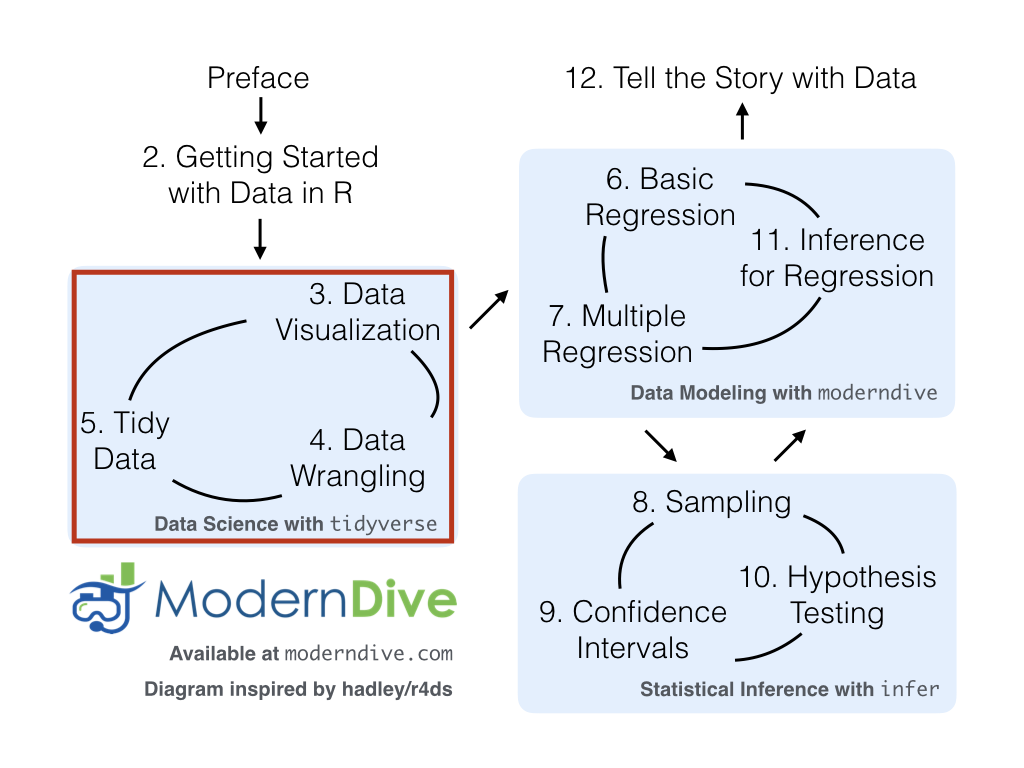
\includegraphics[width=1.1\linewidth]{images/flowcharts/flowchart/flowchart.004} 

}

\caption{ModernDive flowchart}\label{fig:unnamed-chunk-10}
\end{figure}

\part{Data Science via the
tidyverse}\label{part-data-science-via-the-tidyverse}

\chapter{Data Visualization via ggplot2}\label{viz}

We begin the development of your data science toolbox with data
visualization. By visualizing our data, we will be able to gain valuable
insights from our data that we couldn't initially see from just looking
at the raw data in spreadsheet form. We will use the \texttt{ggplot2}
package as it provides an easy way to customize your plots and is rooted
in the data visualization theory known as \emph{The Grammar of Graphics}
\citep{wilkinson2005}.

At the most basic level, graphics/plots/charts (we use these terms
interchangeably in this book) provide a nice way for us to get a sense
for how quantitative variables compare in terms of their center (where
the values tend to be located) and their spread (how they vary around
the center). The most important thing to know about graphics is that
they should be created to make it obvious for your audience to
understand the findings and insight you want to get across. This does
however require a balancing act. On the one hand, you want to highlight
as many meaningful relationships and interesting findings as possible,
but on the other you don't want to include so many as to overwhelm your
audience.

As we will see, plots/graphics also help us to identify patterns and
outliers in our data. We will see that a common extension of these ideas
is to compare the \emph{distribution} of one quantitative variable
(i.e., what the spread of a variable looks like or how the variable is
\emph{distributed} in terms of its values) as we go across the levels of
a different categorical variable.

\subsection*{Needed packages}\label{needed-packages}


Let's load all the packages needed for this chapter (this assumes you've
already installed them). Read Section \ref{packages} for information on
how to install and load R packages.

\begin{Shaded}
\begin{Highlighting}[]
\KeywordTok{library}\NormalTok{(nycflights13)}
\KeywordTok{library}\NormalTok{(ggplot2)}
\KeywordTok{library}\NormalTok{(dplyr)}
\end{Highlighting}
\end{Shaded}

\subsection*{DataCamp}\label{datacamp}


Our approach to introducing data visualization via the Grammar of
Graphics and the \texttt{ggplot2} package is very similar to the
approach taken in \href{https://twitter.com/drob}{David Robinson's}
DataCamp course ``Introduction to the Tidyverse,'' a course targeted at
people new to R and the tidyverse. If you're interested in complementing
your learning below in an interactive online environment, click on the
image below to access the course. The relevant chapters of the course
are Chapter 2 on ``Data visualization'' and Chapter 4 on ``Types of
visualizations.''

\href{https://www.datacamp.com/courses/introduction-to-the-tidyverse}{
\includegraphics[width=0.2\textwidth]{images/datacamp_intro_to_tidyverse.png}}

\section{The Grammar of Graphics}\label{grammarofgraphics}

We begin with a discussion of a theoretical framework for data
visualization known as the ``The Grammar of Graphics,'' which serves as
the basis for the \texttt{ggplot2} package. Much like how we construct
sentences in any language by using a linguistic grammar (nouns, verbs,
subjects, objects, etc.), the theoretical framework given by Leland
Wilkinson \citep{wilkinson2005} allows us to specify the components of a
statistical graphic.

\subsection{Components of the Grammar}\label{components-of-the-grammar}

In short, the grammar tells us that:

\begin{quote}
\textbf{A statistical graphic is a \texttt{mapping} of \texttt{data}
variables to \texttt{aes}thetic attributes of \texttt{geom}etric
objects.}
\end{quote}

Specifically, we can break a graphic into the following three essential
components:

\begin{enumerate}
\def\labelenumi{\arabic{enumi}.}
\tightlist
\item
  \texttt{data}: the data-set comprised of variables that we map.
\item
  \texttt{geom}: the geometric object in question. This refers to our
  type of objects we can observe in our plot. For example, points,
  lines, bars, etc.
\item
  \texttt{aes}: aesthetic attributes of the geometric object that we can
  perceive on a graphic. For example, x/y position, color, shape, and
  size. Each assigned aesthetic attribute can be mapped to a variable in
  our data-set.
\end{enumerate}

Let's break down the grammar with an example.

\subsection{Gapminder}\label{gapminder}

In February 2006, a statistician named Hans Rosling gave a TED talk
titled
\href{https://www.ted.com/talks/hans_rosling_shows_the_best_stats_you_ve_ever_seen}{``The
best stats you've ever seen''} where he presented global economic,
health, and development data from the website
\href{http://www.gapminder.org/tools/\#_locale_id=en;\&chart-type=bubbles}{gapminder.org}.
For example, from the 1704 countries included from 2007, consider only
the first 6 countries when listed alphabetically:

\begin{table}

\caption{\label{tab:unnamed-chunk-16}Gapminder 2007 Data: First 6 of 142 countries}
\centering
\fontsize{10}{12}\selectfont
\begin{tabular}[t]{llrrr}
\toprule
Country & Continent & Life Expectancy & Population & GDP per Capita\\
\midrule
Afghanistan & Asia & 43.83 & 31889923 & 974.58\\
Albania & Europe & 76.42 & 3600523 & 5937.03\\
Algeria & Africa & 72.30 & 33333216 & 6223.37\\
Angola & Africa & 42.73 & 12420476 & 4797.23\\
Argentina & Americas & 75.32 & 40301927 & 12779.38\\
Australia & Oceania & 81.23 & 20434176 & 34435.37\\
\bottomrule
\end{tabular}
\end{table}

Each row in this table corresponds to a country in 2007. For each row,
we have 5 columns:

\begin{enumerate}
\def\labelenumi{\arabic{enumi}.}
\tightlist
\item
  \textbf{Country}: Name of country.
\item
  \textbf{Continent}: Which of the five continents the country is part
  of. (Note that \texttt{Americas} groups North and South America and
  that Antarctica is excluded here.)
\item
  \textbf{Life Expectancy}: Life expectancy in years.
\item
  \textbf{Population}: Number of people living in the country.
\item
  \textbf{GDP per Capita}: Gross domestic product (in US dollars).
\end{enumerate}

Now consider Figure \ref{fig:gapminder}, which plots this data for all
142 countries in the data frame. Note that R will deal with large
numbers using scientific notation. So in the legend for ``Population'',
1.25e+09 = \(1.25 \times 10^{9}\) = 1,250,000,000 = 1.25 billion.

\begin{figure}

{\centering 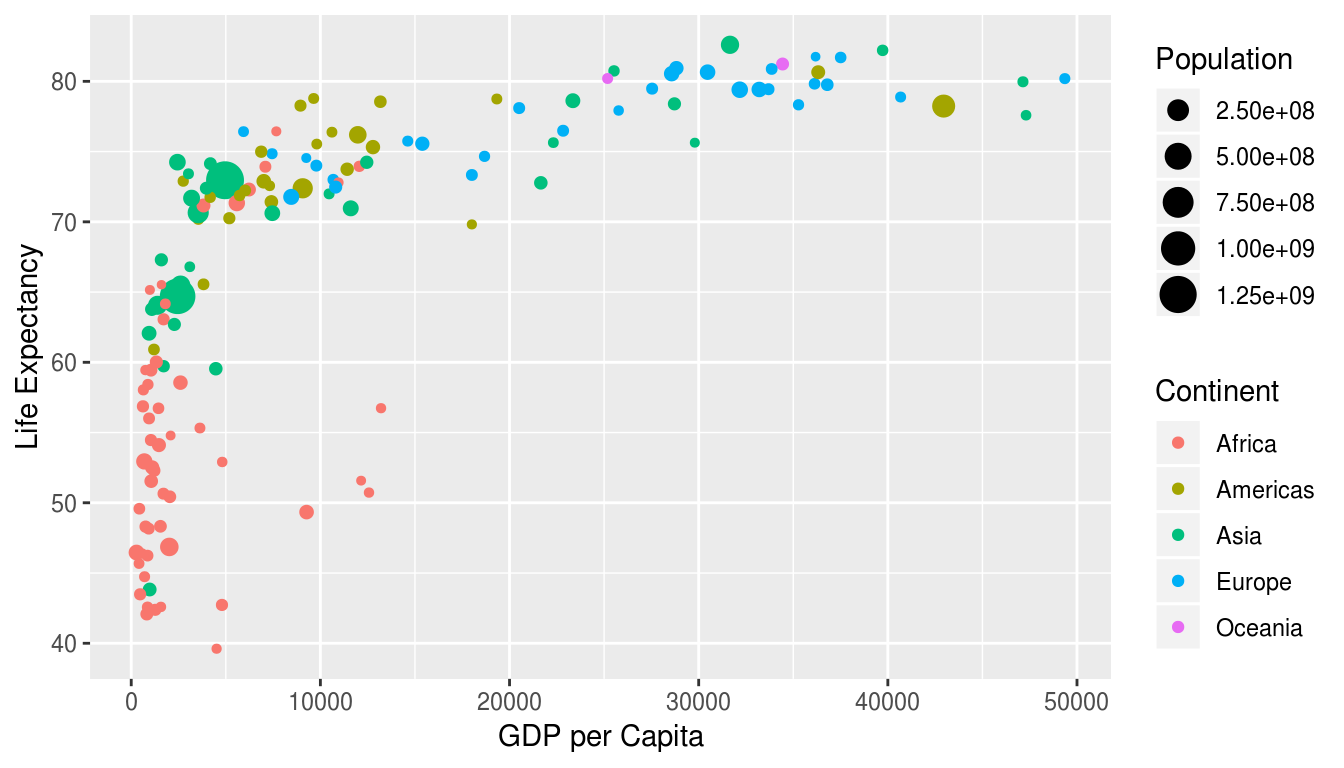
\includegraphics[width=\textwidth]{ismaykim_files/figure-latex/gapminder-1} 

}

\caption{Life Expectancy over GDP per Capita in 2007}\label{fig:gapminder}
\end{figure}

Let's view this plot through the grammar of graphics:

\begin{enumerate}
\def\labelenumi{\arabic{enumi}.}
\tightlist
\item
  The \texttt{data} variable \textbf{GDP per Capita} gets mapped to the
  \texttt{x}-position \texttt{aes}thetic of the points.
\item
  The \texttt{data} variable \textbf{Life Expectancy} gets mapped to the
  \texttt{y}-position \texttt{aes}thetic of the points.
\item
  The \texttt{data} variable \textbf{Population} gets mapped to the
  \texttt{size} \texttt{aes}thetic of the points.
\item
  The \texttt{data} variable \textbf{Continent} gets mapped to the
  \texttt{color} \texttt{aes}thetic of the points.
\end{enumerate}

Recall that \texttt{data} here corresponds to each of the variables
being in the same \texttt{data} frame and the ``data variable''
corresponds to a column in a data frame.

While in this example we are considering one type of \texttt{geom}etric
object (of type \texttt{point}), graphics are not limited to just
points. Some plots involve lines while others involve bars. Let's
summarize the three essential components of the grammar in a table:

\begin{table}

\caption{\label{tab:unnamed-chunk-17}Summary of Grammar of Graphics for this plot}
\centering
\fontsize{10}{12}\selectfont
\begin{tabular}[t]{lll}
\toprule
data variable & aes & geom\\
\midrule
GDP per Capita & x & point\\
Life Expectancy & y & point\\
Population & size & point\\
Continent & color & point\\
\bottomrule
\end{tabular}
\end{table}

\subsection{Other components of the
Grammar}\label{other-components-of-the-grammar}

There are other components of the Grammar of Graphics we can control. As
you start to delve deeper into the Grammar of Graphics, you'll start to
encounter these topics more and more often. In this book, we'll only
work with the two other components below (The other components are left
to a more advanced text such as
\href{http://r4ds.had.co.nz/data-visualisation.html\#aesthetic-mappings}{R
for Data Science} \citep{rds2016}):

\begin{itemize}
\tightlist
\item
  \texttt{facet}ing breaks up a plot into small multiples corresponding
  to the levels of another variable (Section \ref{facets})
\item
  \texttt{position} adjustments for barplots (Section \ref{geombar}) 
\end{itemize}

In general, the Grammar of Graphics allows for a high degree of
customization and also a consistent framework for easy
updating/modification of plots.

\subsection{The ggplot2 package}\label{the-ggplot2-package}

In this book, we will be using the \texttt{ggplot2} package for data
visualization, which is an implementation of the Grammar of Graphics for
R \citep{R-ggplot2}. You may have noticed that a lot of the previous
text in this chapter is written in computer font. This is because the
various components of the Grammar of Graphics are specified in the
\texttt{ggplot} function, which expects at a bare minimum as arguments:

\begin{itemize}
\tightlist
\item
  The data frame where the variables exist: the \texttt{data} argument
\item
  The mapping of the variables to aesthetic attributes: the
  \texttt{mapping} argument, which specifies the \texttt{aes}thetic
  attributes involved
\end{itemize}

After we've specified these components, we then add \emph{layers} to the
plot using the \texttt{+} sign. The most essential layer to add to a
plot is the specification of which type of \texttt{geom}etric object we
want the plot to involve; e.g.~points, lines, bars. Other layers we can
add include the specification of the plot title, axes labels, facets,
and visual themes for the plot.

Let's now put the theory of the Grammar of Graphics into practice.

\section{Five Named Graphs - The 5NG}\label{FiveNG}

For our purposes, we will be limiting consideration to five different
types of graphs. We term these five named graphs the \textbf{5NG}:

\begin{enumerate}
\def\labelenumi{\arabic{enumi}.}
\tightlist
\item
  scatterplots
\item
  linegraphs
\item
  boxplots
\item
  histograms
\item
  barplots
\end{enumerate}

We will discuss some variations of these plots, but with this basic
repertoire in your toolbox you can visualize a wide array of different
data variable types. Note that certain plots are only appropriate for
categorical/logical variables and others only for quantitative
variables. You'll want to quiz yourself often as we go along on which
plot makes sense a given a particular problem or data-set.

\section{5NG\#1: Scatterplots}\label{scatterplots}

The simplest of the 5NG are \emph{scatterplots} (also called bivariate
plots); they allow you to investigate the relationship between two
numerical variables. While you may already be familiar with this type of
plot, let's view it through the lens of the Grammar of Graphics.
Specifically, we will graphically investigate the relationship between
the following two numerical variables in the \texttt{flights} data
frame:

\begin{enumerate}
\def\labelenumi{\arabic{enumi}.}
\tightlist
\item
  \texttt{dep\_delay}: departure delay on the horizontal ``x'' axis and
\item
  \texttt{arr\_delay}: arrival delay on the vertical ``y'' axis
\end{enumerate}

for Alaska Airlines flights leaving NYC in 2013. This requires paring
down the \texttt{flights} data frame to a smaller data frame
\texttt{all\_alaska\_flights} consisting of only Alaska Airlines
(carrier code ``AS'') flights. Don't worry for now if you don't fully
understand what this code is doing, we'll explain this in details
Chapter \ref{wrangling}, just run it all and understand that we are
taking all flights and only considering those corresponding to Alaska
Airlines.

\begin{Shaded}
\begin{Highlighting}[]
\NormalTok{all_alaska_flights <-}\StringTok{ }\NormalTok{flights }\OperatorTok\StringTok{ }
\StringTok{  }\KeywordTok{filter}\NormalTok{(carrier }\OperatorTok{==}\StringTok{ "AS"}\NormalTok{)}
\end{Highlighting}
\end{Shaded}

This code snippet makes use of functions in the \texttt{dplyr} package
for data wrangling to achieve our goal: it takes the \texttt{flights}
data frame and \texttt{filter}s it to only return the rows which meet
the condition \texttt{carrier\ ==\ "AS"}. Recall from Section \ref{code}
that testing for equality is specified with \texttt{==} and not
\texttt{=}. You will see many more examples of \texttt{==} and
\texttt{filter()} in Chapter \ref{wrangling}.

\begin{learncheck}
\textbf{\emph{Learning check}}
\end{learncheck}

\textbf{(LC3.1)} Take a look at both the \texttt{flights} and
\texttt{all\_alaska\_flights} data frames by running
\texttt{View(flights)} and \texttt{View(all\_alaska\_flights)} in the
console. In what respect do these data frames differ?

\begin{learncheck}

\end{learncheck}

\subsection{Scatterplots via geom\_point}\label{geompoint}

We proceed to create the scatterplot using the \texttt{ggplot()}
function:

\begin{Shaded}
\begin{Highlighting}[]
\KeywordTok{ggplot}\NormalTok{(}\DataTypeTok{data =}\NormalTok{ all_alaska_flights, }
       \DataTypeTok{mapping =} \KeywordTok{aes}\NormalTok{(}\DataTypeTok{x =}\NormalTok{ dep_delay, }\DataTypeTok{y =}\NormalTok{ arr_delay)) }\OperatorTok{+}\StringTok{ }
\StringTok{  }\KeywordTok{geom_point}\NormalTok{()}
\end{Highlighting}
\end{Shaded}

\begin{figure}

{\centering 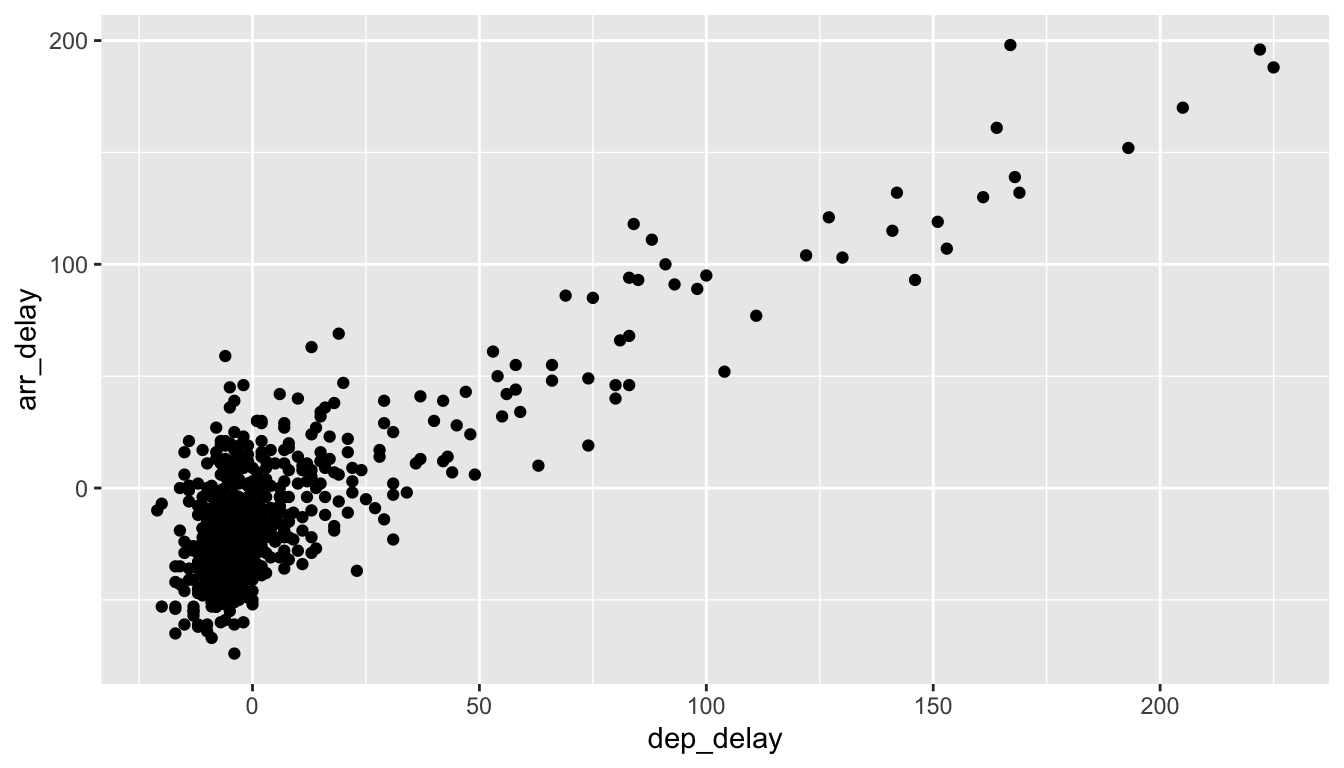
\includegraphics[width=\textwidth]{ismaykim_files/figure-latex/noalpha-1} 

}

\caption{Arrival Delays vs Departure Delays for Alaska Airlines flights from NYC in 2013}\label{fig:noalpha}
\end{figure}

In Figure \ref{fig:noalpha} we see that a positive relationship exists
between \texttt{dep\_delay} and \texttt{arr\_delay}: as departure delays
increase, arrival delays tend to also increase. We also note that the
majority of points fall near the point (0, 0). There is a large mass of
points clustered there. Furthermore after executing this code, R returns
a warning message alerting us to the fact that 5 rows were ignored due
to missing values. For 5 rows either the value for \texttt{dep\_delay}
or \texttt{arr\_delay} or both were missing, and thus these rows were
ignored in our plot.

Let's go back to the \texttt{ggplot()} function call that created this
visualization, keeping in mind our discussion in Section
\ref{grammarofgraphics}:

\begin{itemize}
\tightlist
\item
  Within the \texttt{ggplot()} function call, we specify two of the
  components of the grammar:

  \begin{enumerate}
  \def\labelenumi{\arabic{enumi}.}
  \tightlist
  \item
    The \texttt{data} frame to be \texttt{all\_alaska\_flights} by
    setting \texttt{data\ =\ all\_alaska\_flights}
  \item
    The \texttt{aes}thetic \texttt{mapping} by setting
    \texttt{aes(x\ =\ dep\_delay,\ y\ =\ arr\_delay)}. Specifically

    \begin{itemize}
    \tightlist
    \item
      the variable \texttt{dep\_delay} maps to the \texttt{x} position
      aesthetic
    \item
      the variable \texttt{arr\_delay} maps to the \texttt{y} position
      aesthetic
    \end{itemize}
  \end{enumerate}
\item
  We add a layer to the \texttt{ggplot()} function call using the
  \texttt{+} sign. The layer in question specifies the third component
  of the grammar: the \texttt{geom}etric object. In this case the
  geometric object are \texttt{point}s, set by specifying
  \texttt{geom\_point()}.
\end{itemize}

Some notes on layers:

\begin{itemize}
\tightlist
\item
  Note that the \texttt{+} sign comes at the end of lines, and not at
  the beginning. You'll get an error in R if you put it at the
  beginning.
\item
  When adding layers to a plot, you are encouraged to hit \emph{Return}
  on your keyboard after entering the \texttt{+} so that the code for
  each layer is on a new line. As we add more and more layers to plots,
  you'll see this will greatly improve the legibility of your code.
\item
  To stress the importance of adding layers, in particular the layer
  specifying the \texttt{geom}etric object, consider Figure
  \ref{fig:nolayers} where no layers are added. A not very useful plot!
\end{itemize}

\begin{Shaded}
\begin{Highlighting}[]
\KeywordTok{ggplot}\NormalTok{(}\DataTypeTok{data =}\NormalTok{ all_alaska_flights, }
       \DataTypeTok{mapping =} \KeywordTok{aes}\NormalTok{(}\DataTypeTok{x =}\NormalTok{ dep_delay, }\DataTypeTok{y =}\NormalTok{ arr_delay))}
\end{Highlighting}
\end{Shaded}

\begin{figure}

{\centering 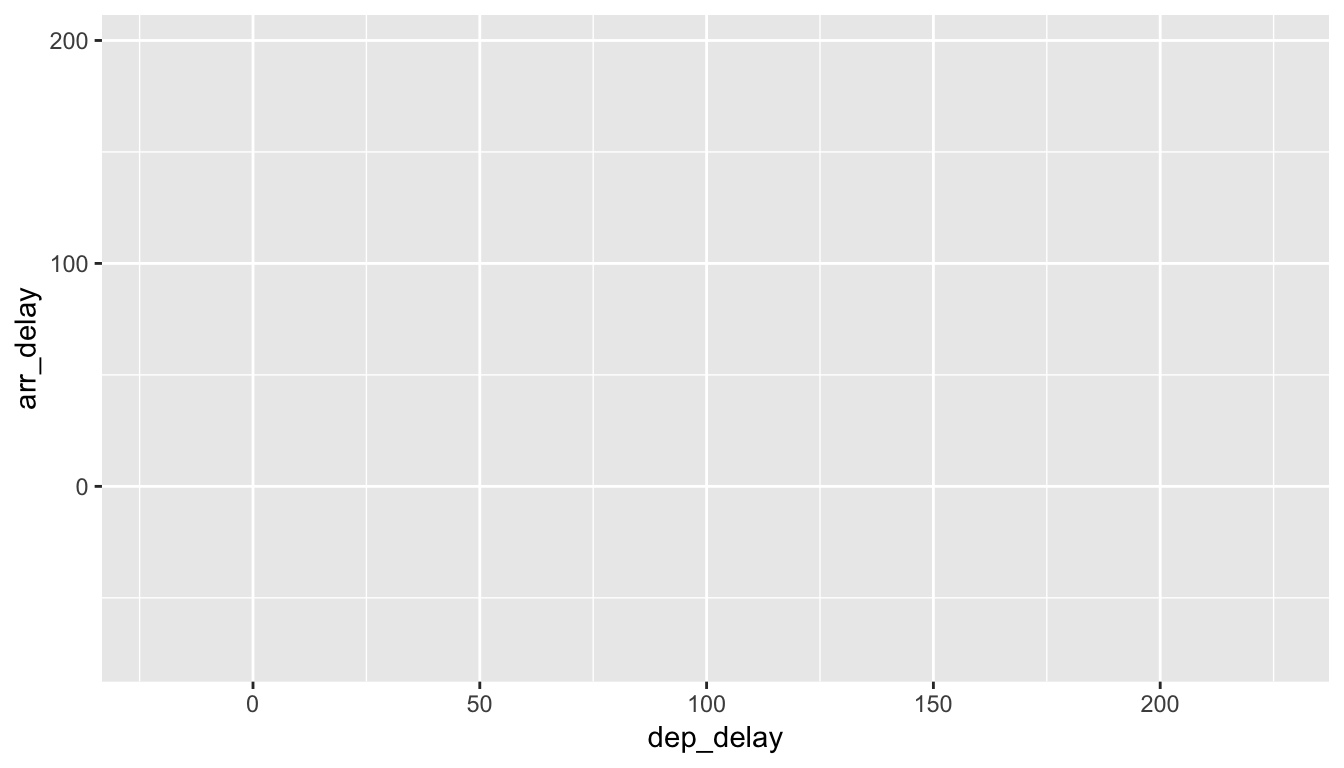
\includegraphics[width=\textwidth]{ismaykim_files/figure-latex/nolayers-1} 

}

\caption{Plot with No Layers}\label{fig:nolayers}
\end{figure}

\begin{learncheck}
\textbf{\emph{Learning check}}
\end{learncheck}

\textbf{(LC3.2)} What are some practical reasons why \texttt{dep\_delay}
and \texttt{arr\_delay} have a positive relationship?

\textbf{(LC3.3)} What variables (not necessarily in the \texttt{flights}
data frame) would you expect to have a negative correlation (i.e.~a
negative relationship) with \texttt{dep\_delay}? Why? Remember that we
are focusing on numerical variables here.

\textbf{(LC3.4)} Why do you believe there is a cluster of points near
(0, 0)? What does (0, 0) correspond to in terms of the Alaskan flights?

\textbf{(LC3.5)} What are some other features of the plot that stand out
to you?

\textbf{(LC3.6)} Create a new scatterplot using different variables in
the \texttt{all\_alaska\_flights} data frame by modifying the example
above.

\begin{learncheck}

\end{learncheck}

\subsection{Over-plotting}\label{overplotting}

The large mass of points near (0, 0) in Figure \ref{fig:noalpha} can
cause some confusion. This is the result of a phenomenon called
\emph{overplotting}. As one may guess, this corresponds to values being
plotted on top of each other \emph{over} and \emph{over} again. It is
often difficult to know just how many values are plotted in this way
when looking at a basic scatterplot as we have here. There are two ways
to address this issue:

\begin{enumerate}
\def\labelenumi{\arabic{enumi}.}
\tightlist
\item
  By adjusting the transparency of the points via the \texttt{alpha}
  argument
\item
  By jittering the points via \texttt{geom\_jitter()}
\end{enumerate}

The first way of relieving overplotting is by changing the
\texttt{alpha} argument in \texttt{geom\_point()} which controls the
transparency of the points. By default, this value is set to \texttt{1}.
We can change this to any value between \texttt{0} and \texttt{1} where
\texttt{0} sets the points to be 100\% transparent and \texttt{1} sets
the points to be 100\% opaque. Note how the following function call is
identical to the one in Section \ref{scatterplots}, but with
\texttt{alpha\ =\ 0.2} added to the \texttt{geom\_point()}.

\begin{Shaded}
\begin{Highlighting}[]
\KeywordTok{ggplot}\NormalTok{(}\DataTypeTok{data =}\NormalTok{ all_alaska_flights, }
       \DataTypeTok{mapping =} \KeywordTok{aes}\NormalTok{(}\DataTypeTok{x =}\NormalTok{ dep_delay, }\DataTypeTok{y =}\NormalTok{ arr_delay)) }\OperatorTok{+}\StringTok{ }
\StringTok{  }\KeywordTok{geom_point}\NormalTok{(}\DataTypeTok{alpha =} \FloatTok{0.2}\NormalTok{)}
\end{Highlighting}
\end{Shaded}

\begin{figure}

{\centering 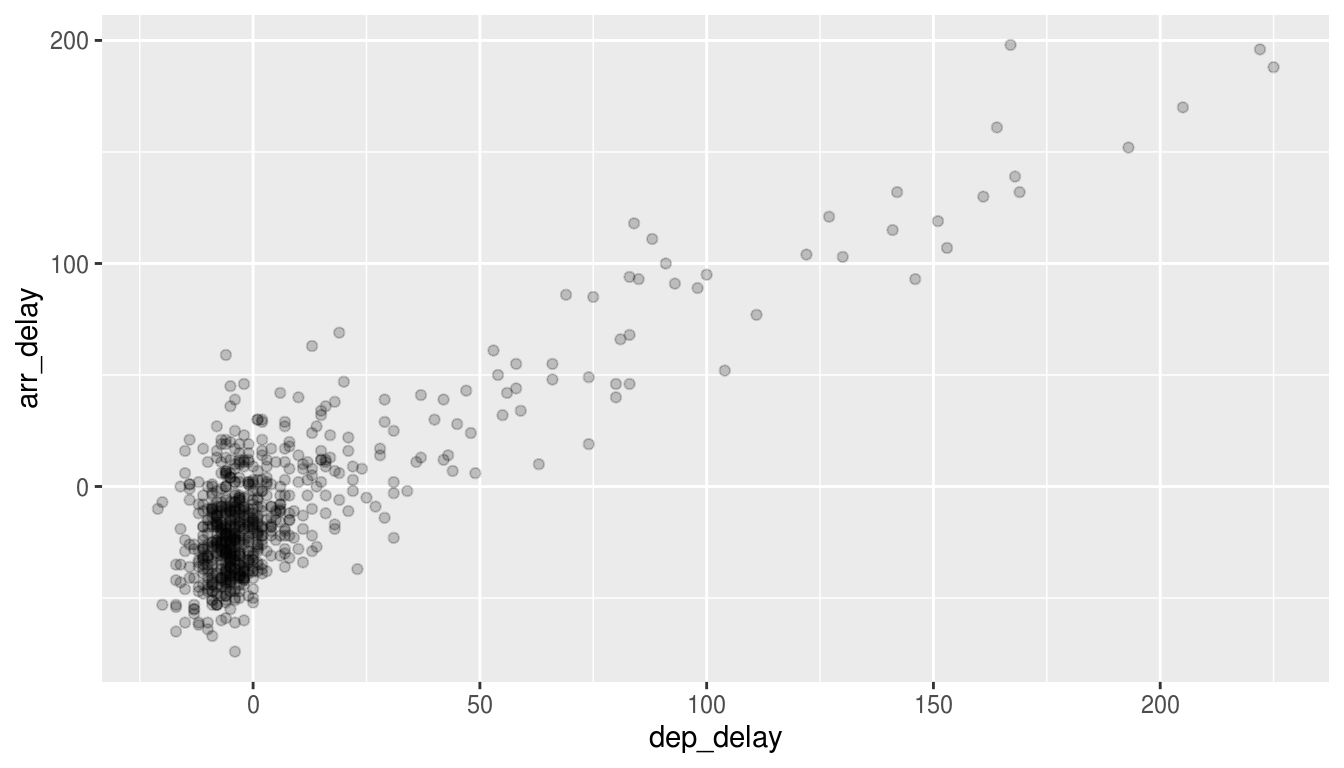
\includegraphics[width=\textwidth]{ismaykim_files/figure-latex/alpha-1} 

}

\caption{Delay scatterplot with alpha=0.2}\label{fig:alpha}
\end{figure}

The key feature to note in Figure \ref{fig:alpha} is that the
transparency of the points is cumulative: areas with a high-degree of
overplotting are darker, whereas areas with a lower degree are less
dark.

Note that there is no \texttt{aes()} surrounding \texttt{alpha\ =\ 0.2}
here. Since we are NOT mapping a variable to an aesthetic but instead
are just changing a setting, we don't need to create a mapping with
\texttt{aes()}. In fact, you'll receive an error if you try to change
the second line above to \texttt{geom\_point(aes(alpha\ =\ 0.2))}.

The second way of relieving overplotting is to \emph{jitter} the points
a bit. In other words, we are going to add just a bit of random noise to
the points to better see them and alleviate some of the overplotting.
You can think of ``jittering'' as shaking the points around a bit on the
plot. Let's illustrate using a simple example first. Say we have a data
frame \texttt{jitter\_example} with 4 rows of identical value 0 for both
\texttt{x} and \texttt{y}:

\begin{Shaded}
\begin{Highlighting}[]
\NormalTok{jitter_example}
\end{Highlighting}
\end{Shaded}

\begin{verbatim}
# A tibble: 4 x 2
      x     y
  <dbl> <dbl>
1     0     0
2     0     0
3     0     0
4     0     0
\end{verbatim}

We display the resulting scatterplot in Figure
\ref{fig:jitter-example-plot-1}; observe that the 4 points are
superimposed on top of each other. While we know there are 4 values
being plotted, this fact might not be apparent to others.

\begin{figure}

{\centering 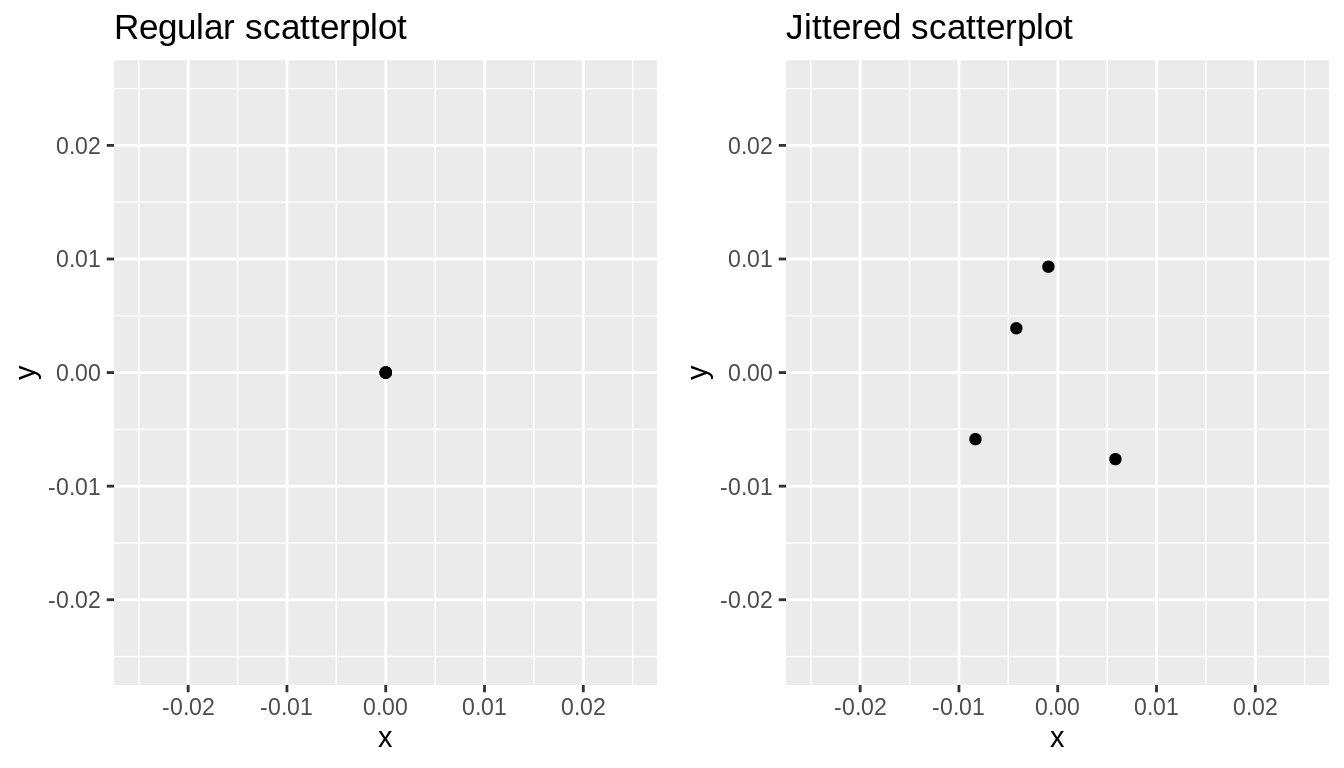
\includegraphics[width=\textwidth]{ismaykim_files/figure-latex/jitter-example-plot-1-1} 

}

\caption{Regular scatterplot of jitter example data}\label{fig:jitter-example-plot-1}
\end{figure}

In Figure \ref{fig:jitter-example-plot-2} we instead display a
\emph{jittered scatterplot}. Since each point is given a random
``nudge'', it is now plainly evident that there are four points.

\begin{figure}

{\centering 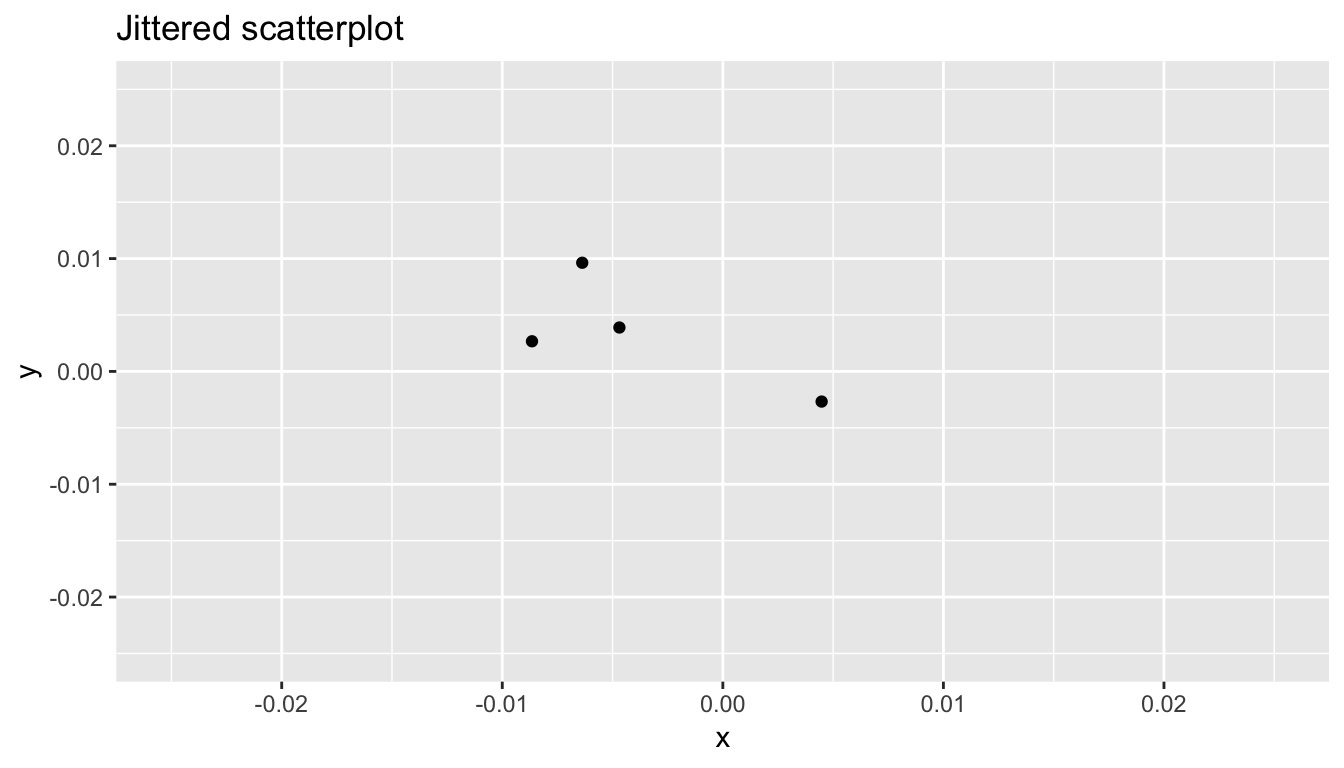
\includegraphics[width=\textwidth]{ismaykim_files/figure-latex/jitter-example-plot-2-1} 

}

\caption{Jittered scatterplot of jitter example data}\label{fig:jitter-example-plot-2}
\end{figure}

To create a jittered scatterplot, instead of using \texttt{geom\_point},
we use \texttt{geom\_jitter}. To specify how much jitter to add, we
adjust the \texttt{width} and \texttt{height} arguments. This
corresponds to how hard you'd like to shake the plot in units
corresponding to those for both the horizontal and vertical variables
(in this case, minutes). It is important to add just enough jitter to
break any overlap in points, but not so much that we completely obscure
the overall pattern in points.

\begin{Shaded}
\begin{Highlighting}[]
\KeywordTok{ggplot}\NormalTok{(}\DataTypeTok{data =}\NormalTok{ all_alaska_flights, }
       \DataTypeTok{mapping =} \KeywordTok{aes}\NormalTok{(}\DataTypeTok{x =}\NormalTok{ dep_delay, }\DataTypeTok{y =}\NormalTok{ arr_delay)) }\OperatorTok{+}\StringTok{ }
\StringTok{  }\KeywordTok{geom_jitter}\NormalTok{(}\DataTypeTok{width =} \DecValTok{30}\NormalTok{, }\DataTypeTok{height =} \DecValTok{30}\NormalTok{)}
\end{Highlighting}
\end{Shaded}

\begin{figure}

{\centering 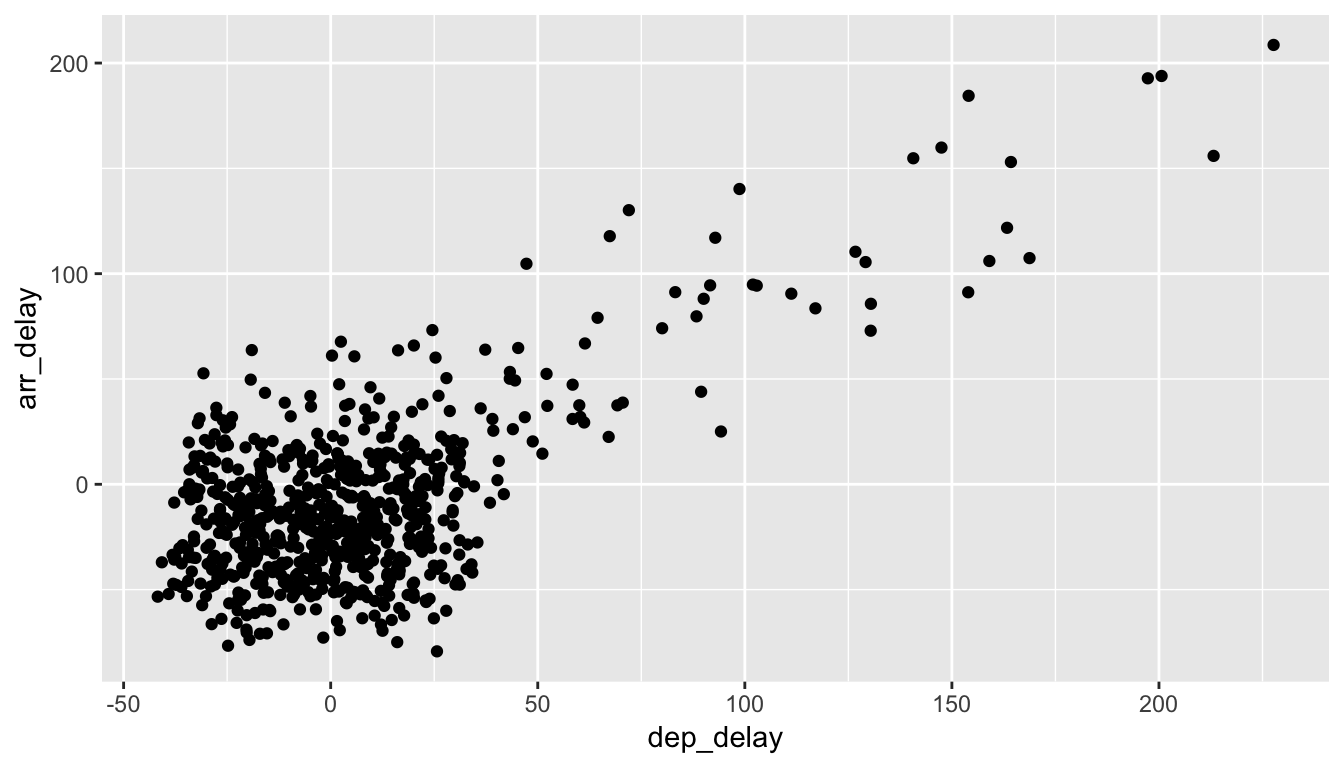
\includegraphics[width=\textwidth]{ismaykim_files/figure-latex/jitter-1} 

}

\caption{Jittered delay scatterplot}\label{fig:jitter}
\end{figure}

Observe how this function call is identical to the one in Subsection
\ref{geompoint}, but with \texttt{geom\_point()} replaced with
\texttt{geom\_jitter()}. Also, it is important to note that
\texttt{geom\_jitter()} is strictly a visualization tool and that does
not alter the original values saved in \texttt{jitter\_example}.

The plot in Figure \ref{fig:jitter} helps us a little bit in getting a
sense for the overplotting, but with a relatively large data-set like
this one (714 flights), it can be argued that changing the transparency
of the points by setting \texttt{alpha} proved more effective.

Furthermore, we'll see later on that the two following R commands will
yield the exact same plot:

\begin{Shaded}
\begin{Highlighting}[]
\KeywordTok{ggplot}\NormalTok{(}\DataTypeTok{data =}\NormalTok{ all_alaska_flights, }
       \DataTypeTok{mapping =} \KeywordTok{aes}\NormalTok{(}\DataTypeTok{x =}\NormalTok{ dep_delay, }\DataTypeTok{y =}\NormalTok{ arr_delay)) }\OperatorTok{+}\StringTok{ }
\StringTok{  }\KeywordTok{geom_jitter}\NormalTok{(}\DataTypeTok{width =} \DecValTok{30}\NormalTok{, }\DataTypeTok{height =} \DecValTok{30}\NormalTok{)}
\KeywordTok{ggplot}\NormalTok{(all_alaska_flights, }\KeywordTok{aes}\NormalTok{(}\DataTypeTok{x =}\NormalTok{ dep_delay, }\DataTypeTok{y =}\NormalTok{ arr_delay)) }\OperatorTok{+}\StringTok{ }
\StringTok{  }\KeywordTok{geom_jitter}\NormalTok{(}\DataTypeTok{width =} \DecValTok{30}\NormalTok{, }\DataTypeTok{height =} \DecValTok{30}\NormalTok{)}
\end{Highlighting}
\end{Shaded}

In other words you can drop the \texttt{data\ =} and \texttt{mapping\ =}
if you keep the order of the two arguments the same. Since the
\texttt{ggplot()} function is expecting its first argument \texttt{data}
to be a data frame and its second argument to correspond to
\texttt{mapping\ =}, you can omit both and you'll get the same plot. As
you get more and more practice, you'll likely find yourself not
including the specification of the argument like this. But for now to
keep things straightforward let's make it a point to include the
\texttt{data\ =} and \texttt{mapping\ =}.

\begin{learncheck}
\textbf{\emph{Learning check}}
\end{learncheck}

\textbf{(LC3.7)} Why is setting the \texttt{alpha} argument value useful
with scatterplots? What further information does it give you that a
regular scatterplot cannot?

\textbf{(LC3.8)} After viewing the Figure \ref{fig:alpha} above, give an
approximate range of arrival delays and departure delays that occur the
most frequently. How has that region changed compared to when you
observed the same plot without the \texttt{alpha\ =\ 0.2} set in Figure
\ref{fig:noalpha}?

\begin{learncheck}

\end{learncheck}

\subsection{Summary}\label{summary}

Scatterplots display the relationship between two numerical variables.
They are among the most commonly used plots because they can provide an
immediate way to see the trend in one variable versus another. However,
if you try to create a scatterplot where either one of the two variables
is not numerical, you will get strange results. Be careful!

With medium to large data-sets, you may need to play with either
\texttt{geom\_jitter()} or the \texttt{alpha} argument in order to get a
good feel for relationships in your data. This tweaking is often a fun
part of data visualization since you'll have the chance to see different
relationships come about as you make subtle changes to your plots.

\section{5NG\#2: Linegraphs}\label{linegraphs}

The next of the 5NG is a linegraph. They are most frequently used when
the x-axis represents time and the y-axis represents some other
numerical variable; such plots are known as \emph{time series}. Time
represents a variable that is connected together by each day following
the previous day. In other words, time has a natural ordering.
Linegraphs should be avoided when there is not a clear sequential
ordering to the explanatory variable, i.e.~the x-variable or the
\emph{predictor} variable.

Our focus now turns to the \texttt{temp} variable in this
\texttt{weather} data-set. By

\begin{itemize}
\tightlist
\item
  Looking over the \texttt{weather} data-set by typing
  \texttt{View(weather)} in the console.
\item
  Running \texttt{?weather} to bring up the help file.
\end{itemize}

We can see that the \texttt{temp} variable corresponds to hourly
temperature (in Fahrenheit) recordings at weather stations near airports
in New York City. Instead of considering all hours in 2013 for all three
airports in NYC, let's focus on the hourly temperature at Newark airport
(\texttt{origin} code ``EWR'') for the first 15 days in January 2013.
The \texttt{weather} data frame in the \texttt{nycflights13} package
contains this data, but we first need to filter it to only include those
rows that correspond to Newark in the first 15 days of January.

\begin{Shaded}
\begin{Highlighting}[]
\NormalTok{early_january_weather <-}\StringTok{ }\NormalTok{weather }\OperatorTok\StringTok{ }
\StringTok{  }\KeywordTok{filter}\NormalTok{(origin }\OperatorTok{==}\StringTok{ "EWR"} \OperatorTok{&}\StringTok{ }\NormalTok{month }\OperatorTok{==}\StringTok{ }\DecValTok{1} \OperatorTok{&}\StringTok{ }\NormalTok{day }\OperatorTok{<=}\StringTok{ }\DecValTok{15}\NormalTok{)}
\end{Highlighting}
\end{Shaded}

This is similar to the previous use of the \texttt{filter} command in
Section \ref{scatterplots}, however we now use the \texttt{\&} operator.
The above selects only those rows in \texttt{weather} where the
originating airport is \texttt{"EWR"} \textbf{and} we are in the first
month \textbf{and} the day is from 1 to 15 inclusive.

\begin{learncheck}
\textbf{\emph{Learning check}}
\end{learncheck}

\textbf{(LC3.9)} Take a look at both the \texttt{weather} and
\texttt{early\_january\_weather} data frames by running
\texttt{View(weather)} and \texttt{View(early\_january\_weather)} in the
console. In what respect do these data frames differ?

\textbf{(LC3.10)} \texttt{View()} the \texttt{flights} data frame again.
Why does the \texttt{time\_hour} variable uniquely identify the hour of
the measurement whereas the \texttt{hour} variable does not?

\begin{learncheck}

\end{learncheck}

\subsection{Linegraphs via geom\_line}\label{geomline}

We plot a linegraph of hourly temperature using \texttt{geom\_line()}:

\begin{Shaded}
\begin{Highlighting}[]
\KeywordTok{ggplot}\NormalTok{(}\DataTypeTok{data =}\NormalTok{ early_january_weather, }
       \DataTypeTok{mapping =} \KeywordTok{aes}\NormalTok{(}\DataTypeTok{x =}\NormalTok{ time_hour, }\DataTypeTok{y =}\NormalTok{ temp)) }\OperatorTok{+}
\StringTok{  }\KeywordTok{geom_line}\NormalTok{()}
\end{Highlighting}
\end{Shaded}

\begin{figure}

{\centering 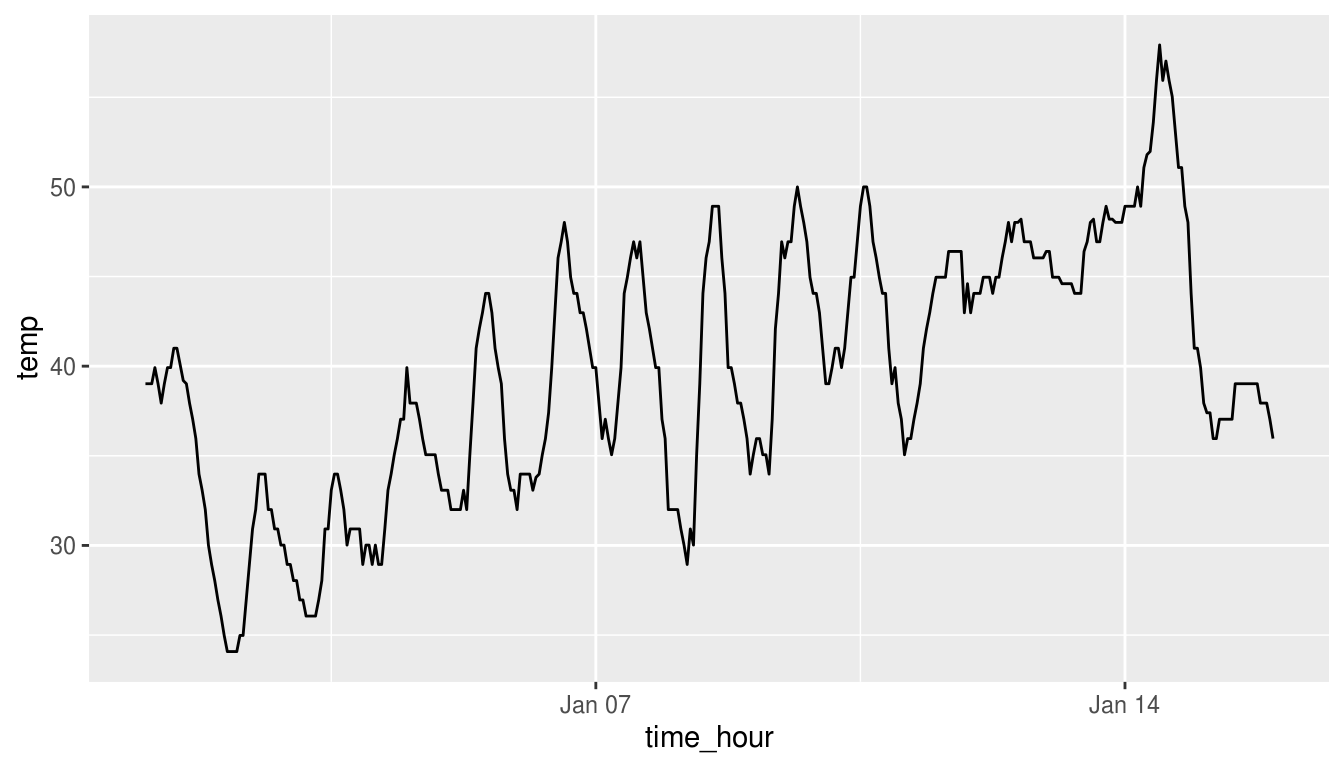
\includegraphics[width=\textwidth]{ismaykim_files/figure-latex/hourlytemp-1} 

}

\caption{Hourly Temperature in Newark for January 1-15, 2013}\label{fig:hourlytemp}
\end{figure}

Much as with the \texttt{ggplot()} call in Chapter \ref{geompoint}, we
describe the components of the Grammar of Graphics:

\begin{itemize}
\tightlist
\item
  Within the \texttt{ggplot()} function call, we specify two of the
  components of the grammar:

  \begin{enumerate}
  \def\labelenumi{\arabic{enumi}.}
  \tightlist
  \item
    The \texttt{data} frame to be \texttt{early\_january\_weather} by
    setting \texttt{data\ =\ early\_january\_weather}
  \item
    The \texttt{aes}thetic mapping by setting
    \texttt{aes(x\ =\ time\_hour,\ y\ =\ temp)}. Specifically

    \begin{itemize}
    \tightlist
    \item
      \texttt{time\_hour} (i.e.~the time variable) maps to the
      \texttt{x} position
    \item
      \texttt{temp} maps to the \texttt{y} position
    \end{itemize}
  \end{enumerate}
\item
  We add a layer to the \texttt{ggplot()} function call using the
  \texttt{+} sign
\item
  The layer in question specifies the third component of the grammar:
  the \texttt{geom}etric object in question. In this case the geometric
  object is a \texttt{line}, set by specifying \texttt{geom\_line()}.
\end{itemize}

\begin{learncheck}
\textbf{\emph{Learning check}}
\end{learncheck}

\textbf{(LC3.11)} Why should linegraphs be avoided when there is not a
clear ordering of the horizontal axis?

\textbf{(LC3.12)} Why are linegraphs frequently used when time is the
explanatory variable?

\textbf{(LC3.13)} Plot a time series of a variable other than
\texttt{temp} for Newark Airport in the first 15 days of January 2013.

\begin{learncheck}

\end{learncheck}

\subsection{Summary}\label{summary-1}

Linegraphs, just like scatterplots, display the relationship between two
numerical variables. However, the variable on the x-axis (i.e.~the
explanatory variable) should have a natural ordering, like some notion
of time. We can mislead our audience if that isn't the case.

\section{5NG\#3: Histograms}\label{histograms}

Let's consider the \texttt{temp} variable in the \texttt{weather} data
frame once again, but now unlike with the linegraphs in Chapter
\ref{linegraphs}, let's say we don't care about the relationship of
temperature to time, but rather we care about the \emph{(statistical)
distribution} of temperatures. We could just produce points where each
of the different values appear on something similar to a number line:

\begin{figure}

{\centering 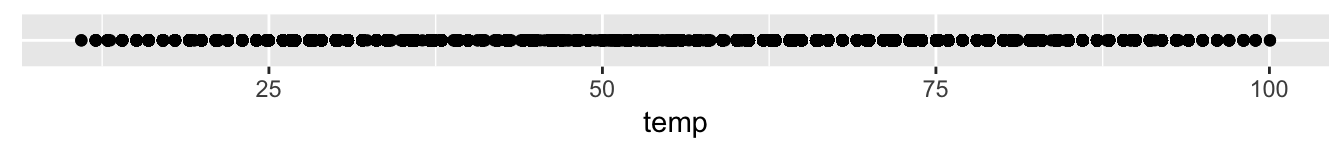
\includegraphics[width=\textwidth]{ismaykim_files/figure-latex/unnamed-chunk-28-1} 

}

\caption{Plot of Hourly Temperature Recordings from NYC in 2013}\label{fig:unnamed-chunk-28}
\end{figure}

This gives us a general idea of how the values of \texttt{temp} differ.
We see that temperatures vary from around 11 up to 100 degrees
Fahrenheit. The area between 40 and 60 degrees appears to have more
points plotted than outside that range.

\subsection{Histograms via geom\_histogram}\label{geomhistogram}

What is commonly produced instead of the above plot is a plot known as a
\emph{histogram}. The histogram shows how many elements of a single
numerical variable fall in specified \emph{bins}. In this case, these
bins may correspond to between 0-10°F, 10-20°F, etc. We produce a
histogram of the hour temperatures at all three NYC airports in 2013:

\begin{Shaded}
\begin{Highlighting}[]
\KeywordTok{ggplot}\NormalTok{(}\DataTypeTok{data =}\NormalTok{ weather, }\DataTypeTok{mapping =} \KeywordTok{aes}\NormalTok{(}\DataTypeTok{x =}\NormalTok{ temp)) }\OperatorTok{+}
\StringTok{  }\KeywordTok{geom_histogram}\NormalTok{()}
\end{Highlighting}
\end{Shaded}

\begin{verbatim}
`stat_bin()` using `bins = 30`. Pick better value with
`binwidth`.
\end{verbatim}

\begin{verbatim}
Warning: Removed 1 rows containing non-finite values (stat_bin).
\end{verbatim}

\begin{figure}

{\centering 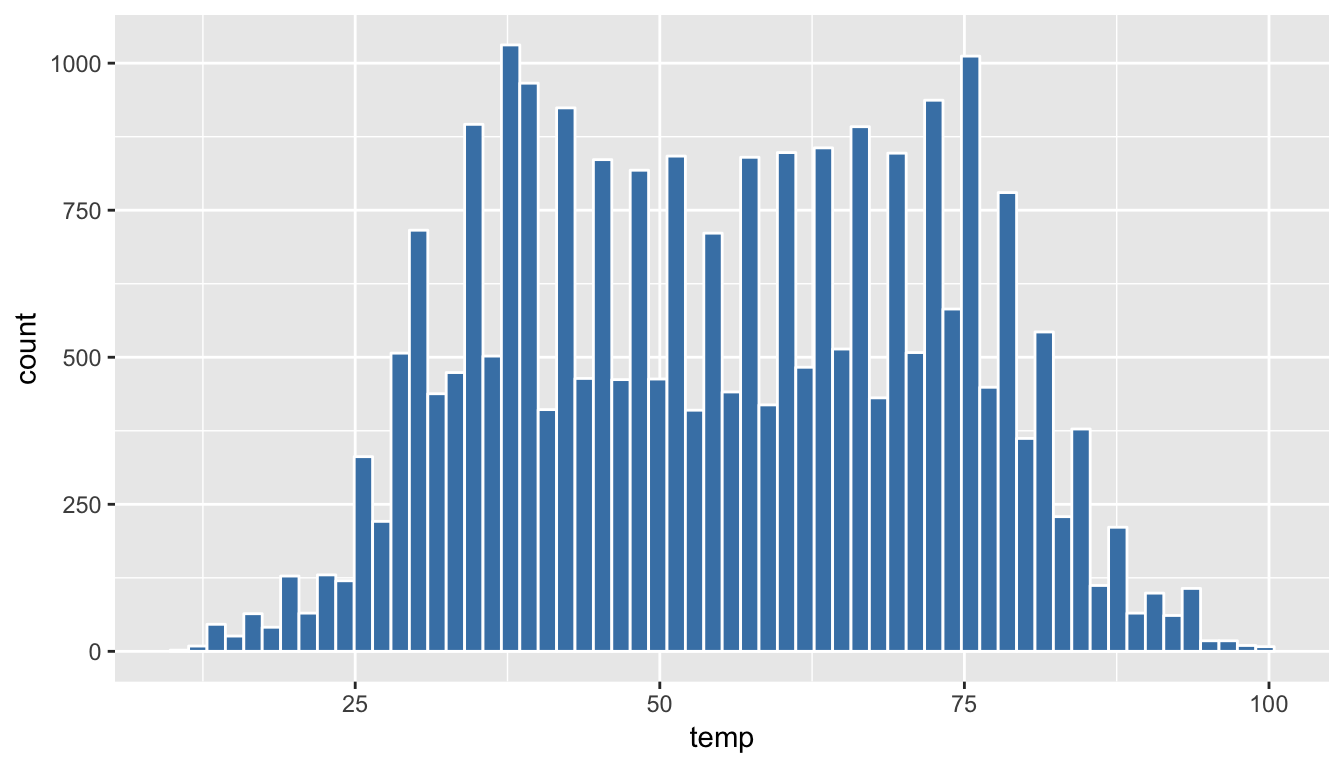
\includegraphics[width=\textwidth]{ismaykim_files/figure-latex/unnamed-chunk-29-1} 

}

\caption{Histogram of Hourly Temperature Recordings from NYC in 2013}\label{fig:unnamed-chunk-29}
\end{figure}

Note here:

\begin{itemize}
\tightlist
\item
  There is only one variable being mapped in \texttt{aes()}: the single
  numerical variable \texttt{temp}. You don't need to compute the
  y-aesthetic: it gets computed automatically.
\item
  We set the \texttt{geom}etric object to be \texttt{geom\_histogram()}
\item
  We got a warning message of
  \texttt{1\ rows\ containing\ non-finite\ values} being removed. This
  is due to one of the values of temperature being missing. R is
  alerting us that this happened.\\
\item
  Another warning corresponds to an urge to specify the number of bins
  you'd like to create.
\end{itemize}

\subsection{Adjusting the bins}\label{adjustbins}

We can adjust characteristics of the bins in one of \emph{two} ways:

\begin{enumerate}
\def\labelenumi{\arabic{enumi}.}
\tightlist
\item
  By adjusting the number of bins via the \texttt{bins} argument
\item
  By adjusting the width of the bins via the \texttt{binwidth} argument
\end{enumerate}

First, we have the power to specify how many bins we would like to put
the data into as an argument in the \texttt{geom\_histogram()} function.
By default, this is chosen to be 30 somewhat arbitrarily; we have
received a warning above our plot that this was done.

\begin{Shaded}
\begin{Highlighting}[]
\KeywordTok{ggplot}\NormalTok{(}\DataTypeTok{data =}\NormalTok{ weather, }\DataTypeTok{mapping =} \KeywordTok{aes}\NormalTok{(}\DataTypeTok{x =}\NormalTok{ temp)) }\OperatorTok{+}
\StringTok{  }\KeywordTok{geom_histogram}\NormalTok{(}\DataTypeTok{bins =} \DecValTok{60}\NormalTok{, }\DataTypeTok{color =} \StringTok{"white"}\NormalTok{)}
\end{Highlighting}
\end{Shaded}

\begin{figure}

{\centering 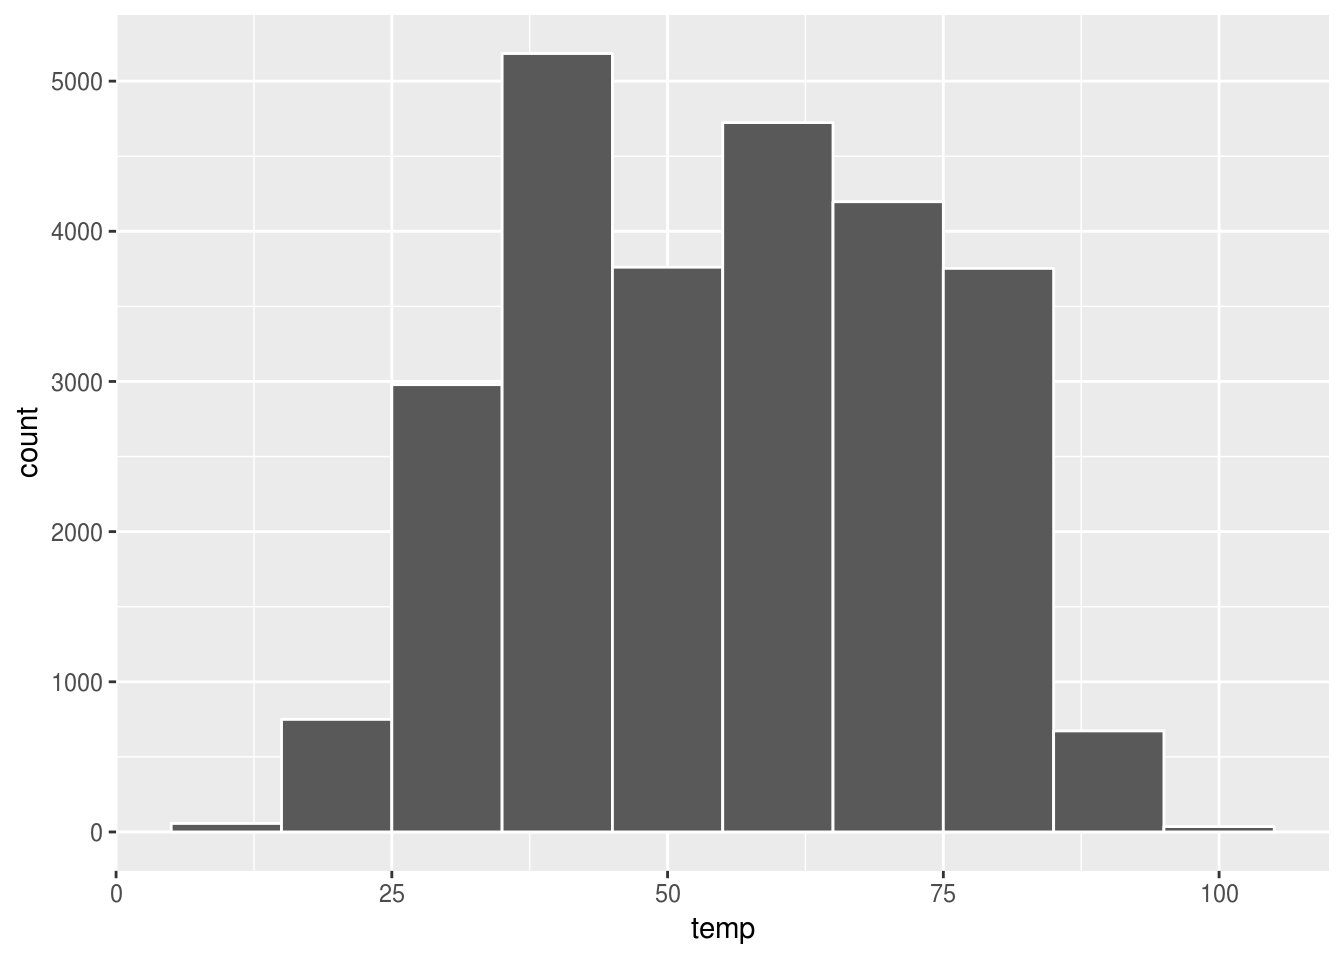
\includegraphics[width=\textwidth]{ismaykim_files/figure-latex/unnamed-chunk-30-1} 

}

\caption{Histogram of Hourly Temperature Recordings from NYC in 2013 - 60 Bins}\label{fig:unnamed-chunk-30}
\end{figure}

Note the addition of the \texttt{color} argument. If you'd like to be
able to more easily differentiate each of the bins, you can specify the
color of the outline as done above. You can also adjust the color of the
bars by setting the \texttt{fill} argument. Type \texttt{colors()} in
your console to see all 657 available colors.

\begin{Shaded}
\begin{Highlighting}[]
\KeywordTok{ggplot}\NormalTok{(}\DataTypeTok{data =}\NormalTok{ weather, }\DataTypeTok{mapping =} \KeywordTok{aes}\NormalTok{(}\DataTypeTok{x =}\NormalTok{ temp)) }\OperatorTok{+}
\StringTok{  }\KeywordTok{geom_histogram}\NormalTok{(}\DataTypeTok{bins =} \DecValTok{60}\NormalTok{, }\DataTypeTok{color =} \StringTok{"white"}\NormalTok{, }\DataTypeTok{fill =} \StringTok{"steelblue"}\NormalTok{)}
\end{Highlighting}
\end{Shaded}

\begin{figure}

{\centering 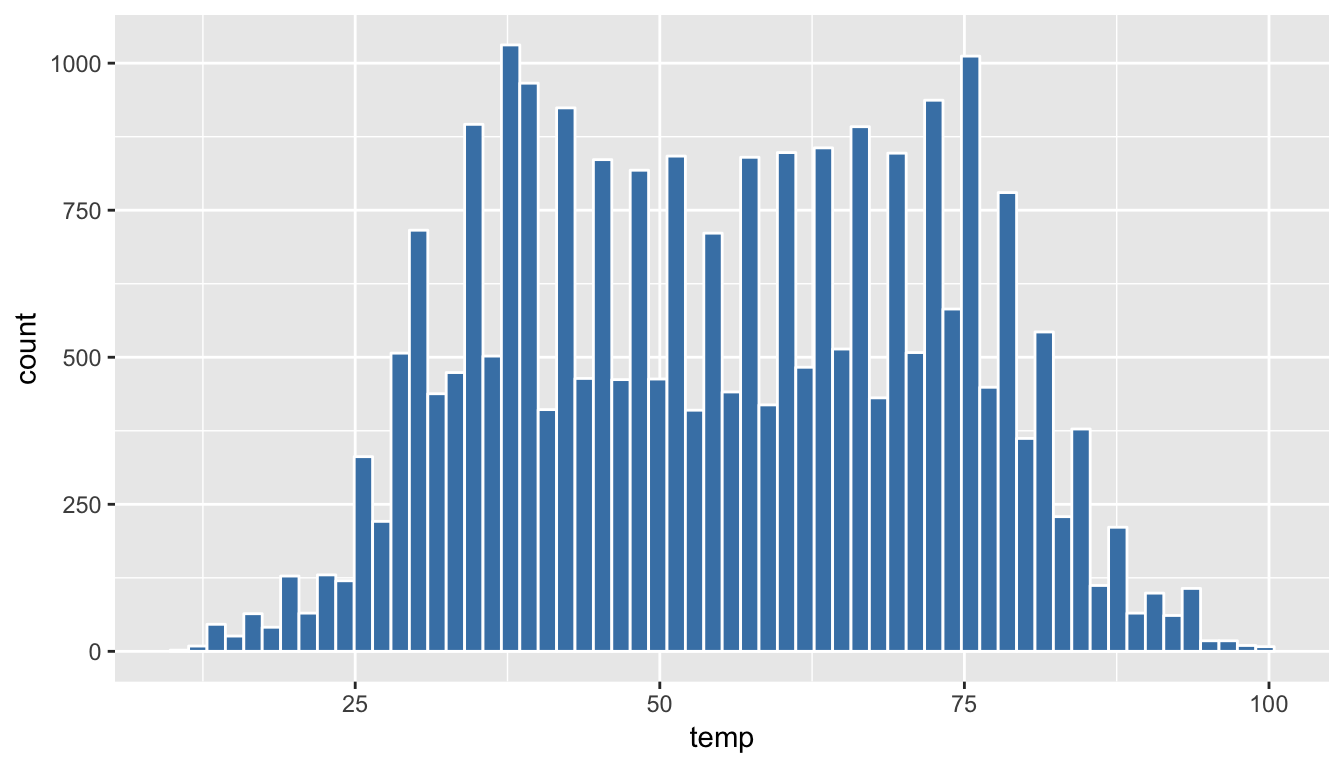
\includegraphics[width=\textwidth]{ismaykim_files/figure-latex/unnamed-chunk-31-1} 

}

\caption{Histogram of Hourly Temperature Recordings from NYC in 2013 - 60 Colored Bins}\label{fig:unnamed-chunk-31}
\end{figure}

Second, instead of specifying the number of bins, we can also specify
the width of the bins by using the \texttt{binwidth} argument in the
\texttt{geom\_histogram} function.

\begin{Shaded}
\begin{Highlighting}[]
\KeywordTok{ggplot}\NormalTok{(}\DataTypeTok{data =}\NormalTok{ weather, }\DataTypeTok{mapping =} \KeywordTok{aes}\NormalTok{(}\DataTypeTok{x =}\NormalTok{ temp)) }\OperatorTok{+}
\StringTok{  }\KeywordTok{geom_histogram}\NormalTok{(}\DataTypeTok{binwidth =} \DecValTok{10}\NormalTok{, }\DataTypeTok{color =} \StringTok{"white"}\NormalTok{)}
\end{Highlighting}
\end{Shaded}

\begin{figure}

{\centering 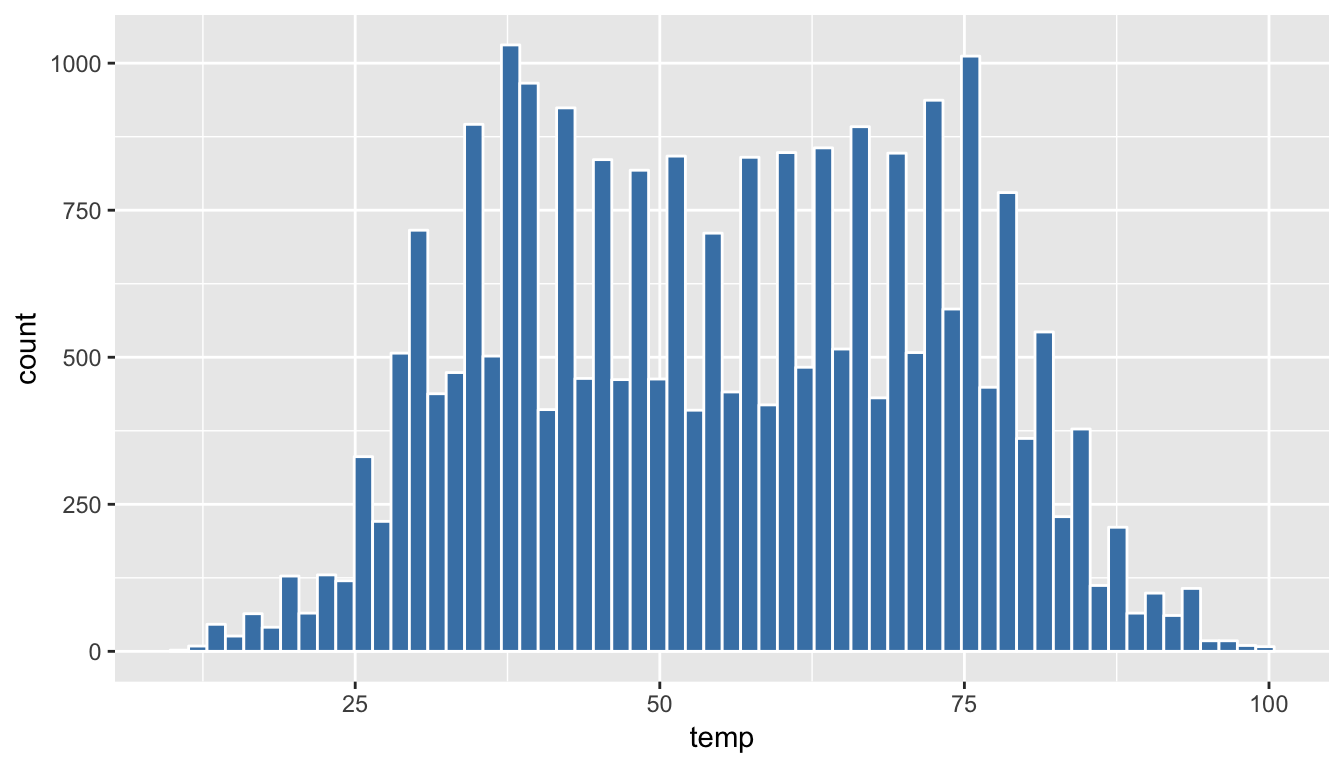
\includegraphics[width=\textwidth]{ismaykim_files/figure-latex/unnamed-chunk-32-1} 

}

\caption{Histogram of Hourly Temperature Recordings from NYC in 2013 - Binwidth = 10}\label{fig:unnamed-chunk-32}
\end{figure}

\begin{learncheck}
\textbf{\emph{Learning check}}
\end{learncheck}

\textbf{(LC3.14)} What does changing the number of bins from 30 to 60
tell us about the distribution of temperatures?

\textbf{(LC3.15)} Would you classify the distribution of temperatures as
symmetric or skewed?

\textbf{(LC3.16)} What would you guess is the ``center'' value in this
distribution? Why did you make that choice?

\textbf{(LC3.17)} Is this data spread out greatly from the center or is
it close? Why?

\begin{learncheck}

\end{learncheck}

\subsection{Summary}\label{summary-2}

Histograms, unlike scatterplots and linegraphs, present information on
only a single numerical variable. In particular they are visualizations
of the (statistical) distribution of values.

\section{Facets}\label{facets}

Before continuing the 5NG, we briefly introduce a new concept called
\emph{faceting}. Faceting is used when we'd like to create small
multiples of the same plot over a different categorical variable. By
default, all of the small multiples will have the same vertical axis.

For example, suppose we were interested in looking at how the
temperature histograms we saw in Chapter \ref{histograms} varied by
month. This is what is meant by ``the distribution of a variable over
another variable'': \texttt{temp} is one variable and \texttt{month} is
the other variable. In order to look at histograms of \texttt{temp} for
each month, we add a layer
\texttt{facet\_wrap(\textasciitilde{}\ month)}. You can also specify how
many rows you'd like the small multiple plots to be in using
\texttt{nrow} or how many columns using \texttt{ncol} inside of
\texttt{facet\_wrap}.

\begin{Shaded}
\begin{Highlighting}[]
\KeywordTok{ggplot}\NormalTok{(}\DataTypeTok{data =}\NormalTok{ weather, }\DataTypeTok{mapping =} \KeywordTok{aes}\NormalTok{(}\DataTypeTok{x =}\NormalTok{ temp)) }\OperatorTok{+}
\StringTok{  }\KeywordTok{geom_histogram}\NormalTok{(}\DataTypeTok{binwidth =} \DecValTok{5}\NormalTok{, }\DataTypeTok{color =} \StringTok{"white"}\NormalTok{) }\OperatorTok{+}
\StringTok{  }\KeywordTok{facet_wrap}\NormalTok{(}\OperatorTok{~}\StringTok{ }\NormalTok{month, }\DataTypeTok{nrow =} \DecValTok{4}\NormalTok{)}
\end{Highlighting}
\end{Shaded}

\begin{figure}

{\centering 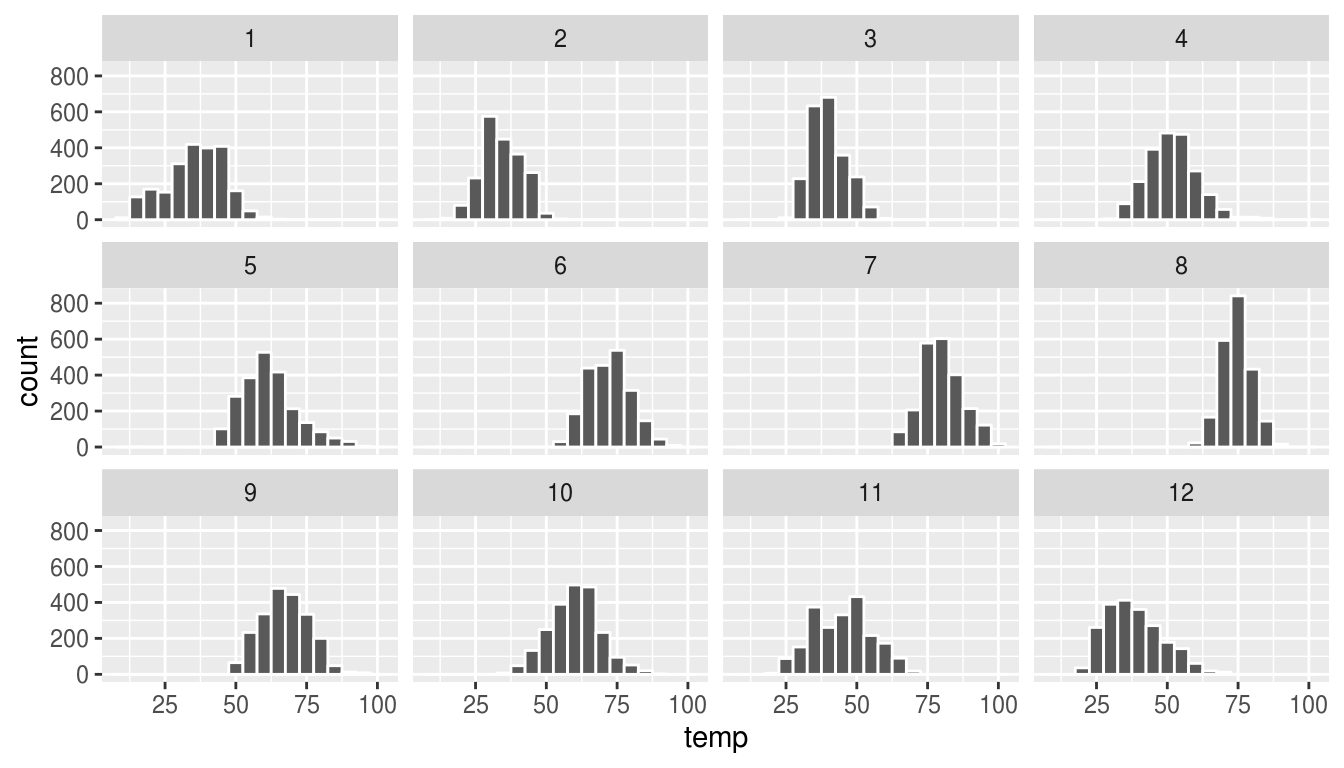
\includegraphics[width=\textwidth]{ismaykim_files/figure-latex/facethistogram-1} 

}

\caption{Faceted histogram}\label{fig:facethistogram}
\end{figure}

Note the use of the \texttt{\textasciitilde{}} before \texttt{month} in
\texttt{facet\_wrap}. The tilde (\texttt{\textasciitilde{}}) is required
and you'll receive the error
\texttt{Error\ in\ as.quoted(facets)\ :\ object\ \textquotesingle{}month\textquotesingle{}\ not\ found}
if you don't include it before \texttt{month} here.

As we might expect, the temperature tends to increase as summer
approaches and then decrease as winter approaches.

\begin{learncheck}
\textbf{\emph{Learning check}}
\end{learncheck}

\textbf{(LC3.18)} What other things do you notice about the faceted plot
above? How does a faceted plot help us see relationships between two
variables?

\textbf{(LC3.19)} What do the numbers 1-12 correspond to in the plot
above? What about 25, 50, 75, 100?

\textbf{(LC3.20)} For which types of data-sets would these types of
faceted plots not work well in comparing relationships between
variables? Give an example describing the nature of these variables and
other important characteristics.

\textbf{(LC3.21)} Does the \texttt{temp} variable in the
\texttt{weather} data-set have a lot of variability? Why do you say
that?

\begin{learncheck}

\end{learncheck}

\section{5NG\#4: Boxplots}\label{boxplots}

While using faceted histograms can provide a way to compare
distributions of a numerical variable split by groups of a categorical
variable as in Section \ref{facets}, an alternative plot called a
\emph{boxplot} (also called a \emph{side-by-side boxplot}) achieves the
same task and is frequently preferred. The \emph{boxplot} uses the
information provided in the \emph{five-number summary} referred to in
Appendix \ref{appendixA}. It gives a way to compare this summary
information across the different levels of a categorical variable.

\subsection{Boxplots via geom\_boxplot}\label{geomboxplot}

Let's create a boxplot to compare the monthly temperatures as we did
above with the faceted histograms.

\begin{Shaded}
\begin{Highlighting}[]
\KeywordTok{ggplot}\NormalTok{(}\DataTypeTok{data =}\NormalTok{ weather, }\DataTypeTok{mapping =} \KeywordTok{aes}\NormalTok{(}\DataTypeTok{x =}\NormalTok{ month, }\DataTypeTok{y =}\NormalTok{ temp)) }\OperatorTok{+}
\StringTok{  }\KeywordTok{geom_boxplot}\NormalTok{()}
\end{Highlighting}
\end{Shaded}

\begin{figure}

{\centering 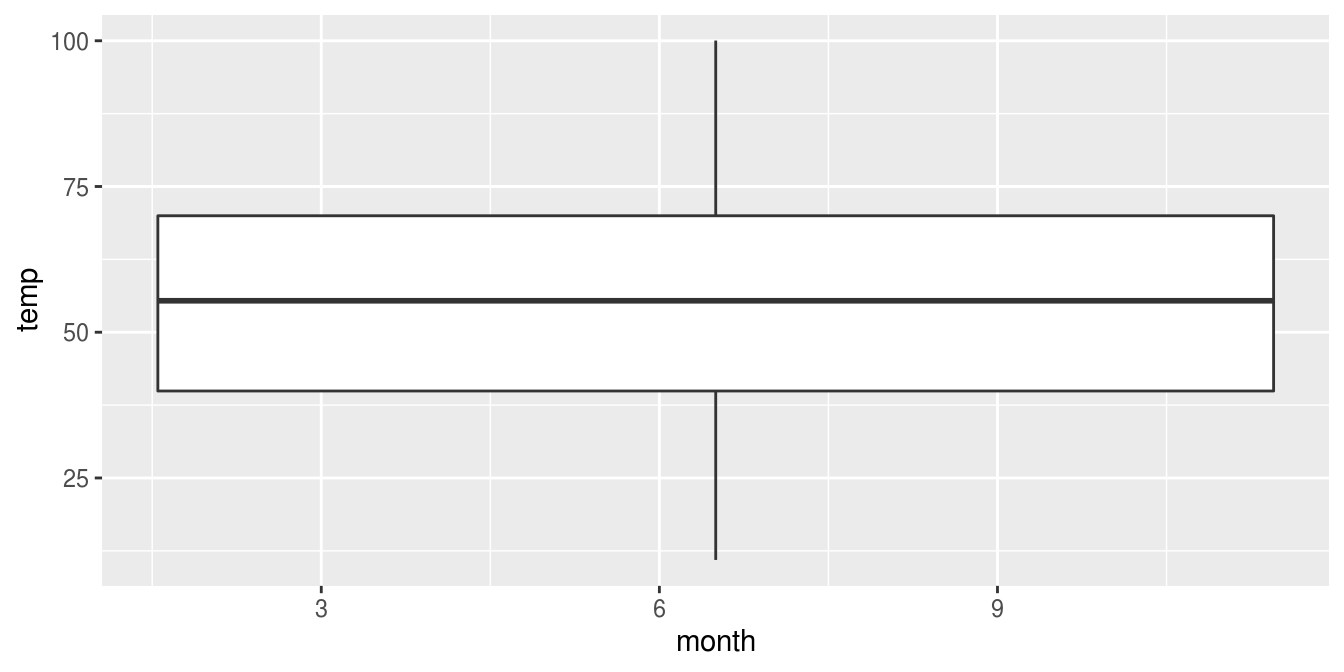
\includegraphics[width=\textwidth]{ismaykim_files/figure-latex/badbox-1} 

}

\caption{Invalid boxplot specification}\label{fig:badbox}
\end{figure}

\begin{verbatim}
Warning messages:
1: Continuous x aesthetic -- did you forget aes(group=...)? 
2: Removed 1 rows containing non-finite values (stat_boxplot). 
\end{verbatim}

Note the set of warnings that is given here. The second warning
corresponds to missing values in the data frame and it is turned off on
subsequent plots. Let's focus on the first warning.

Observe that this plot does not look like what we were expecting. We
were expecting to see the distribution of temperatures for each month
(so 12 different boxplots). The first warning is letting us know that we
are plotting a numerical, and not categorical variable, on the x-axis.
This gives us the overall boxplot without any other groupings. We can
get around this by introducing a new function for our \texttt{x}
variable:

\begin{Shaded}
\begin{Highlighting}[]
\KeywordTok{ggplot}\NormalTok{(}\DataTypeTok{data =}\NormalTok{ weather, }\DataTypeTok{mapping =} \KeywordTok{aes}\NormalTok{(}\DataTypeTok{x =} \KeywordTok{factor}\NormalTok{(month), }\DataTypeTok{y =}\NormalTok{ temp)) }\OperatorTok{+}
\StringTok{  }\KeywordTok{geom_boxplot}\NormalTok{()}
\end{Highlighting}
\end{Shaded}

\begin{figure}

{\centering 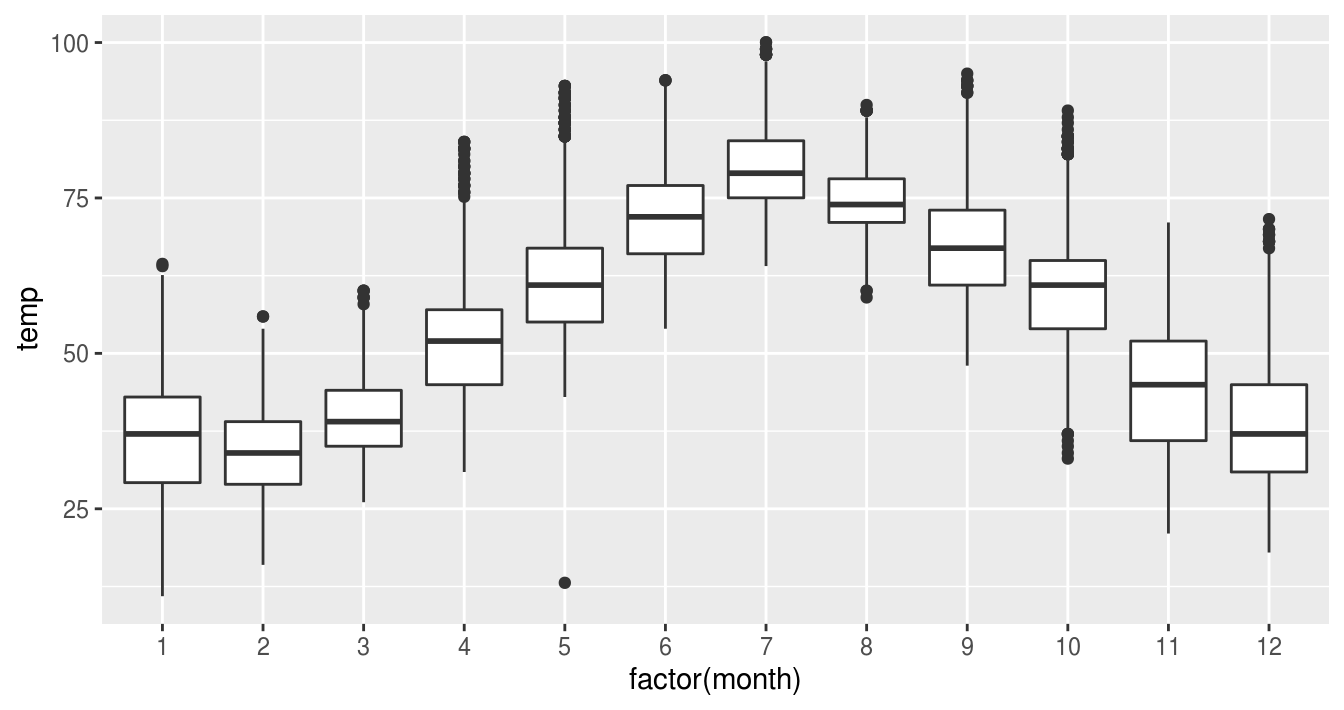
\includegraphics[width=\textwidth]{ismaykim_files/figure-latex/monthtempbox-1} 

}

\caption{Month by temp boxplot}\label{fig:monthtempbox}
\end{figure}

We have introduced a new function called \texttt{factor()} which
converts a numerical variable to a categorical one. This is necessary as
\texttt{geom\_boxplot} requires the \texttt{x} variable to be a
categorical variable, which the variable \texttt{month} is not. So after
applying \texttt{factor(month)}, month goes from having numerical values
1, 2, \ldots{}, 12 to having labels ``1'', ``2'', \ldots{}, ``12.'' The
resulting Figure \ref{fig:monthtempbox} shows 12 separate ``box and
whiskers'' plots with the following features:

\begin{itemize}
\tightlist
\item
  The ``box'' portions of this plot represent the 25\textsuperscript{th}
  percentile AKA the 1\textsuperscript{st} quartile, the median AKA the
  50\textsuperscript{th} percentile AKA the 2\textsuperscript{nd}
  quartile, and the 75\textsuperscript{th} percentile AKA the
  3\textsuperscript{rd} quartile.
\item
  The height of each box, i.e.~the value of the 3\textsuperscript{rd}
  quartile minus the value of the 1\textsuperscript{st} quartile, is
  called the \emph{interquartile range} (\(IQR\)). It is a measure of
  spread of the middle 50\% of values, with longer boxes indicating more
  variability.
\item
  The ``whisker'' portions of these plots extend out from the bottoms
  and tops of the boxes and represent points less than the
  25\textsuperscript{th} percentile and greater than the
  75\textsuperscript{th} percentiles respectively. They're set to extend
  out no more than \(1.5 \times IQR\) units away from either end of the
  boxes. We say ``no more than'' because the ends of the whiskers
  represent the first observed values of \texttt{temp} to be within the
  range of the whiskers. The length of these whiskers show how the data
  outside the middle 50\% of values vary, with longer whiskers
  indicating more variability.
\item
  The dots representing values falling outside the whiskers are called
  \emph{outliers}. It is important to keep in mind that the definition
  of an outlier is somewhat arbitrary and not absolute. In this case,
  they are defined by the length of the whiskers, which are no more than
  \(1.5 \times IQR\) units long.
\end{itemize}

Looking at this plot we can see, as expected, that summer months (6
through 8) have higher median temperatures as evidenced by the higher
solid lines in the middle of the boxes. We can easily compare
temperatures across months by drawing imaginary horizontal lines across
the plot. Furthermore, the height of the 12 boxes as quantified by the
interquartile ranges are informative too; they tell us about
variability, or spread, of temperatures recorded in a given month.

But to really bring home what boxplots show, let's focus only on the
month of November's 2141 temperature recordings.

\begin{figure}

{\centering 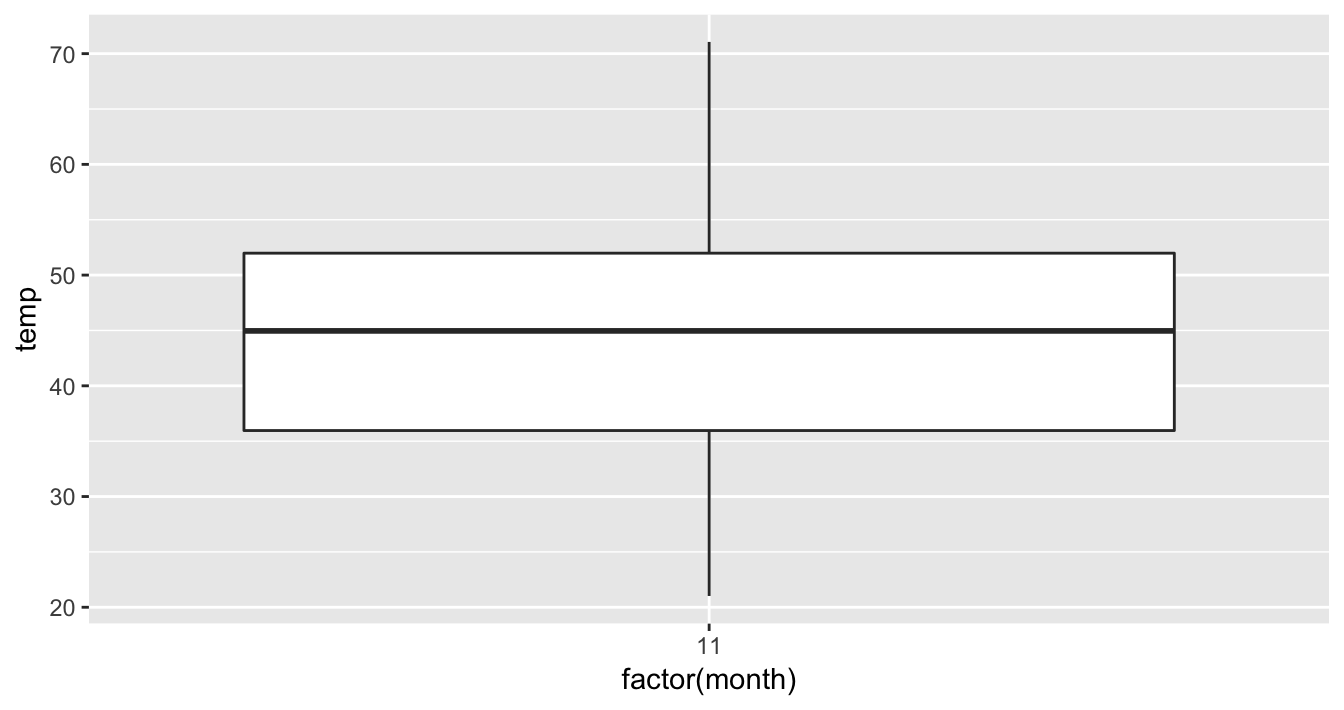
\includegraphics[width=\textwidth]{ismaykim_files/figure-latex/monthtempbox2-1} 

}

\caption{November boxplot}\label{fig:monthtempbox2}
\end{figure}

Now let's plot all 2141 temperature recordings for November on top of
the boxplot in Figure \ref{fig:monthtempbox3}.

\begin{figure}

{\centering 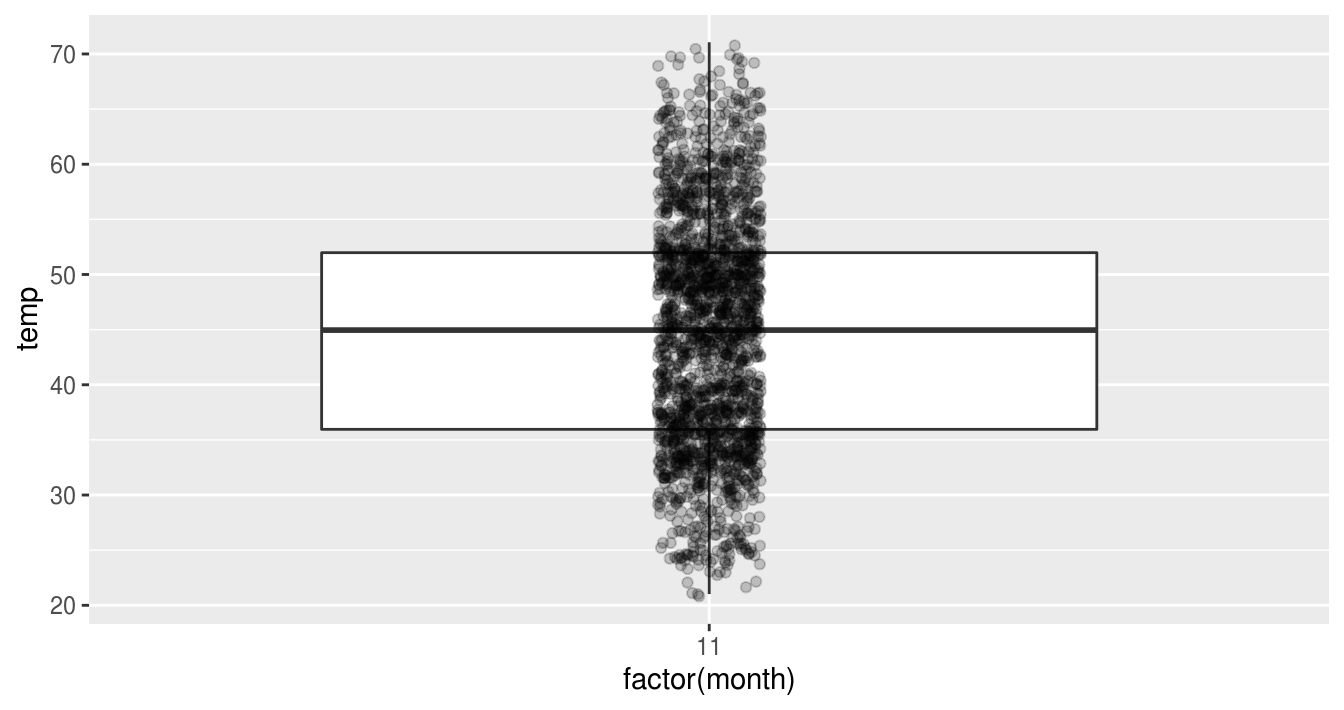
\includegraphics[width=\textwidth]{ismaykim_files/figure-latex/monthtempbox3-1} 

}

\caption{November boxplot with points}\label{fig:monthtempbox3}
\end{figure}

What the boxplot does is summarize the 2141 points for you, in
particular:

\begin{enumerate}
\def\labelenumi{\arabic{enumi}.}
\tightlist
\item
  25\% of points (about 534 observations) fall below the bottom edge of
  the box which is the first quartile of 35.96 degrees Fahrenheit (2.2
  degrees Celsius). In other words 25\% of observations were colder than
  35.96 degrees Fahrenheit.
\item
  25\% of points fall between the bottom edge of the box and the solid
  middle line which is the median of 44.96 degrees Fahrenheit (7.8
  degrees Celsius). In other words 25\% of observations were between
  35.96 and 44.96 degrees Fahrenheit.
\item
  25\% of points fall between the solid middle line and the top edge of
  the box which is the third quartile of 51.98 degrees Fahrenheit (11.1
  degrees Celsius). In other words 25\% of observations were between
  44.96 and 51.98 degrees Fahrenheit.
\item
  25\% of points fall over the top edge of the box. In other words 25\%
  of observations were warmer than 51.98 degrees Fahrenheit.
\item
  The middle 50\% of points lie within the interquartile range 16.02
  degrees Fahrenheit.
\end{enumerate}

\begin{learncheck}
\textbf{\emph{Learning check}}
\end{learncheck}

\textbf{(LC3.22)} What does the dot at the bottom of the plot for May
correspond to? Explain what might have occurred in May to produce this
point.

\textbf{(LC3.23)} Which months have the highest variability in
temperature? What reasons do you think this is?

\textbf{(LC3.24)} We looked at the distribution of a numerical variable
over a categorical variable here with this boxplot. Why can't we look at
the distribution of one numerical variable over the distribution of
another numerical variable? Say, temperature across pressure, for
example?

\textbf{(LC3.25)} Boxplots provide a simple way to identify outliers.
Why may outliers be easier to identify when looking at a boxplot instead
of a faceted histogram?

\begin{learncheck}

\end{learncheck}

\subsection{Summary}\label{summary-3}

Boxplots provide a way to compare and contrast the distribution of one
quantitative variable across multiple levels of one categorical
variable. One can see where the median falls across the different groups
by looking at the center line in the box. To see how spread out the
variable is across the different groups, look at both the width of the
box and also how far the lines stretch vertically from the box. (If the
lines stretch far from the box but the box has a small width, the
variability of the values closer to the center is much smaller than the
variability of the outer ends of the variable.) Outliers are even more
easily identified when looking at a boxplot than when looking at a
histogram.

\section{5NG\#5: Barplots}\label{geombar}

Both histograms and boxplots represent ways to visualize the variability
of numerical variables. Another common task is to present the
distribution of a categorical variable. This is a simpler task, focused
on how many elements from the data fall into different categories of the
categorical variable. Often the best way to visualize these different
counts (also known as \emph{frequencies}) is via a barplot, also known
as a barchart.

One complication, however, is how your data is represented: is the
categorical variable of interest ``pre-counted'' or not? For example,
run the following code in your Console. This code manually creates two
data frames representing a collection of fruit: 3 apples and 2 oranges.

\begin{Shaded}
\begin{Highlighting}[]
\NormalTok{fruits <-}\StringTok{ }\KeywordTok{data_frame}\NormalTok{(}
  \DataTypeTok{fruit =} \KeywordTok{c}\NormalTok{(}\StringTok{"apple"}\NormalTok{, }\StringTok{"apple"}\NormalTok{, }\StringTok{"apple"}\NormalTok{, }\StringTok{"orange"}\NormalTok{, }\StringTok{"orange"}\NormalTok{)}
\NormalTok{)}
\NormalTok{fruits_counted <-}\StringTok{ }\KeywordTok{data_frame}\NormalTok{(}
  \DataTypeTok{fruit =} \KeywordTok{c}\NormalTok{(}\StringTok{"apple"}\NormalTok{, }\StringTok{"orange"}\NormalTok{),}
  \DataTypeTok{number =} \KeywordTok{c}\NormalTok{(}\DecValTok{3}\NormalTok{, }\DecValTok{2}\NormalTok{)}
\NormalTok{)}
\end{Highlighting}
\end{Shaded}

We see both the \texttt{fruits} and \texttt{fruits\_counted} data frames
represent the same collection of fruit. Whereas \texttt{fruits} just
lists the fruit individually:

\begin{table}

\caption{\label{tab:fruits}Fruits}
\centering
\fontsize{10}{12}\selectfont
\begin{tabular}[t]{l}
\toprule
fruit\\
\midrule
apple\\
apple\\
apple\\
orange\\
orange\\
\bottomrule
\end{tabular}
\end{table}

\texttt{fruits\_counted} has a variable \texttt{count} which represents
pre-counted values of each fruit.

\begin{table}

\caption{\label{tab:fruitscounted}Fruits (Pre-Counted)}
\centering
\fontsize{10}{12}\selectfont
\begin{tabular}[t]{lr}
\toprule
fruit & number\\
\midrule
apple & 3\\
orange & 2\\
\bottomrule
\end{tabular}
\end{table}

\subsection{Barplots via
geom\_bar/geom\_col}\label{barplots-via-geom_bargeom_col}

Let's generate barplots using these two different representations of the
same basket of fruit: 3 apples and 2 oranges. Using the not pre-counted
data \texttt{fruits} from Table \ref{tab:fruits}:

\begin{Shaded}
\begin{Highlighting}[]
\KeywordTok{ggplot}\NormalTok{(}\DataTypeTok{data =}\NormalTok{ fruits, }\DataTypeTok{mapping =} \KeywordTok{aes}\NormalTok{(}\DataTypeTok{x =}\NormalTok{ fruit)) }\OperatorTok{+}
\StringTok{  }\KeywordTok{geom_bar}\NormalTok{()}
\end{Highlighting}
\end{Shaded}

\begin{figure}

{\centering 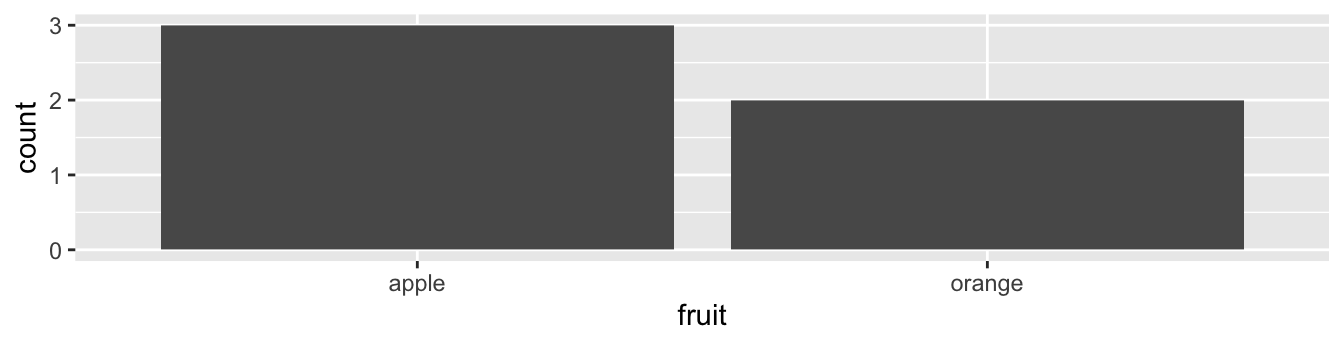
\includegraphics[width=\textwidth]{ismaykim_files/figure-latex/geombar-1} 

}

\caption{Barplot when counts are not pre-counted}\label{fig:geombar}
\end{figure}

and using the pre-counted data \texttt{fruits\_counted} from Table
\ref{tab:fruitscounted}:

\begin{Shaded}
\begin{Highlighting}[]
\KeywordTok{ggplot}\NormalTok{(}\DataTypeTok{data =}\NormalTok{ fruits_counted, }\DataTypeTok{mapping =} \KeywordTok{aes}\NormalTok{(}\DataTypeTok{x =}\NormalTok{ fruit, }\DataTypeTok{y =}\NormalTok{ number)) }\OperatorTok{+}
\StringTok{  }\KeywordTok{geom_col}\NormalTok{()}
\end{Highlighting}
\end{Shaded}

\begin{figure}

{\centering 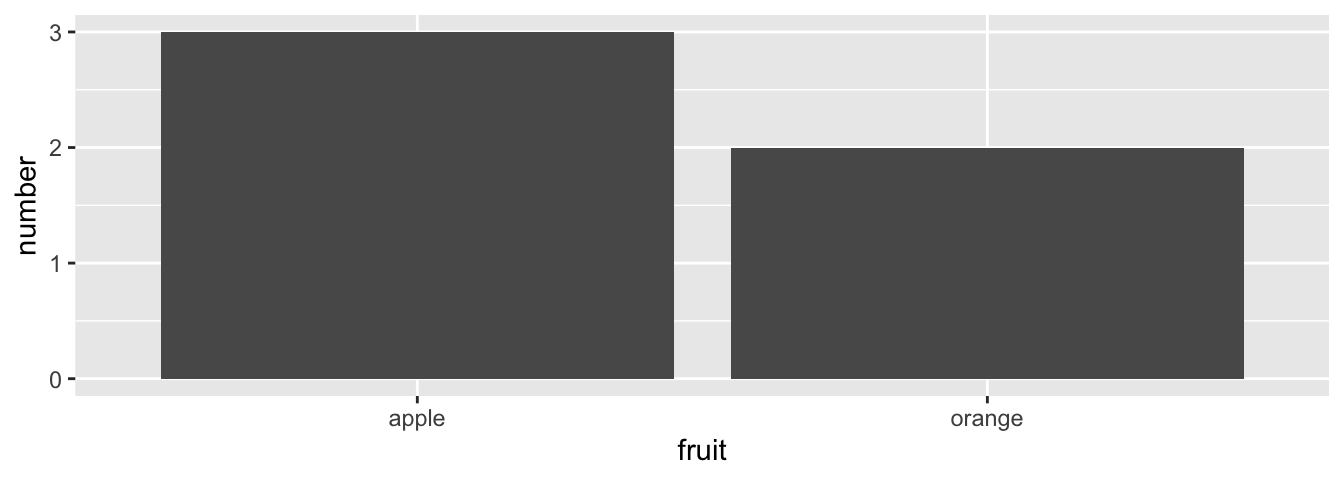
\includegraphics[width=\textwidth]{ismaykim_files/figure-latex/geomcol-1} 

}

\caption{Barplot when counts are pre-counted}\label{fig:geomcol}
\end{figure}

Compare the barplots in Figures \ref{fig:geombar} and \ref{fig:geomcol},
which are identical, but are based on the two different data frames.
Observe that:

\begin{itemize}
\tightlist
\item
  The code that generates Figure \ref{fig:geombar} based on
  \texttt{fruits} does not map a variable to the \texttt{y}
  \texttt{aes}thetic and uses \texttt{geom\_bar()}.
\item
  The code that generates Figure \ref{fig:geomcol} based on
  \texttt{fruits\_counted} maps the \texttt{number} variable to the
  \texttt{y} \texttt{aes}thetic and uses \texttt{geom\_col()}
\end{itemize}

Stating the above differently:

\begin{itemize}
\tightlist
\item
  When the categorical variable you want to plot is not pre-counted in
  your data frame you need to use \texttt{geom\_bar()}.
\item
  When the categorical variable is pre-counted (in the above
  \texttt{fruits\_counted} example in the variable \texttt{number}), you
  need to use \texttt{geom\_col()} with the \texttt{y} aesthetic
  explicitly mapped.
\end{itemize}

Please note that understanding this difference is one of
\texttt{ggplot2}'s trickier aspects that causes the most confusion, and
fortunately this is as complicated as our use of \texttt{ggplot2} is
going to get. Let's consider a different distribution: the distribution
of airlines that flew out of New York City in 2013. Here we explore the
number of flights from each airline/\texttt{carrier}. This can be
plotted by invoking the \texttt{geom\_bar} function in \texttt{ggplot2}:




\begin{Shaded}
\begin{Highlighting}[]
\KeywordTok{ggplot}\NormalTok{(}\DataTypeTok{data =}\NormalTok{ flights, }\DataTypeTok{mapping =} \KeywordTok{aes}\NormalTok{(}\DataTypeTok{x =}\NormalTok{ carrier)) }\OperatorTok{+}
\StringTok{  }\KeywordTok{geom_bar}\NormalTok{()}
\end{Highlighting}
\end{Shaded}

\begin{figure}

{\centering 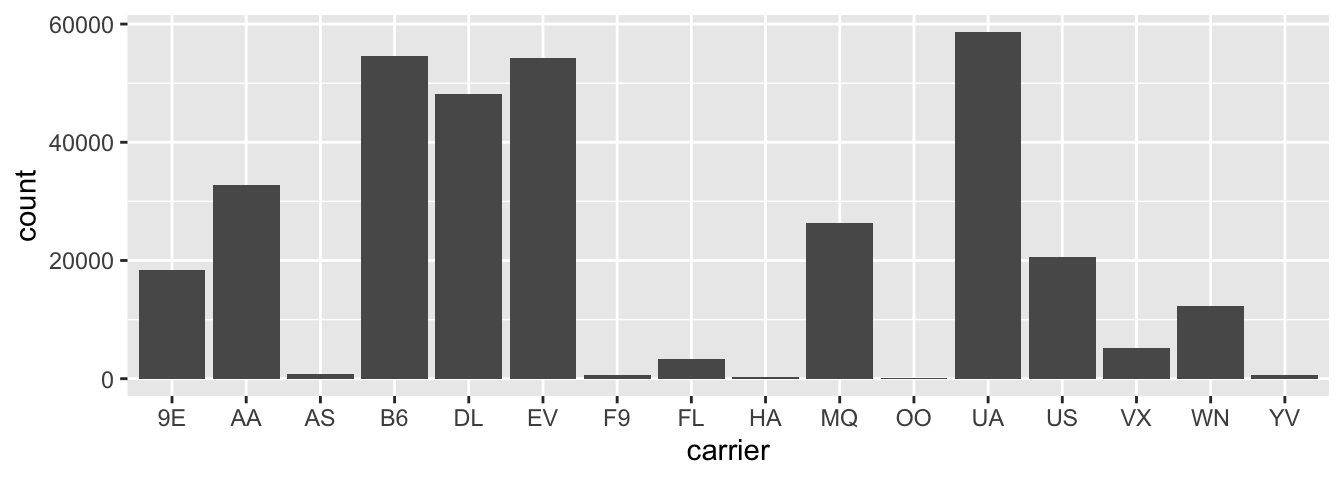
\includegraphics[width=\textwidth]{ismaykim_files/figure-latex/flightsbar-1} 

}

\caption{Number of flights departing NYC in 2013 by airline using
geom\_bar}\label{fig:flightsbar}
\end{figure}

To get an understanding of what the names of these airlines are
corresponding to these \texttt{carrier} codes, we can look at the
\texttt{airlines} data frame in the \texttt{nycflights13} package.

\begin{Shaded}
\begin{Highlighting}[]
\NormalTok{airlines}
\end{Highlighting}
\end{Shaded}

\begin{table}[H]
\centering\begingroup\fontsize{10}{12}\selectfont

\begin{tabular}{l|l}
\hline
carrier & name\\
\hline
9E & Endeavor Air Inc.\\
\hline
AA & American Airlines Inc.\\
\hline
AS & Alaska Airlines Inc.\\
\hline
B6 & JetBlue Airways\\
\hline
DL & Delta Air Lines Inc.\\
\hline
EV & ExpressJet Airlines Inc.\\
\hline
F9 & Frontier Airlines Inc.\\
\hline
FL & AirTran Airways Corporation\\
\hline
HA & Hawaiian Airlines Inc.\\
\hline
MQ & Envoy Air\\
\hline
OO & SkyWest Airlines Inc.\\
\hline
UA & United Air Lines Inc.\\
\hline
US & US Airways Inc.\\
\hline
VX & Virgin America\\
\hline
WN & Southwest Airlines Co.\\
\hline
YV & Mesa Airlines Inc.\\
\hline
\end{tabular}
\endgroup{}
\end{table}

Going back to our barplot, we see that United Air Lines, JetBlue
Airways, and ExpressJet Airlines had the most flights depart New York
City in 2013. To get the actual number of flights by each airline we can
use the \texttt{group\_by()}, \texttt{summarize()}, and \texttt{n()}
functions in the \texttt{dplyr} package on the \texttt{carrier} variable
in \texttt{flights}, which we will introduce formally in Chapter
\ref{wrangling}.

\begin{Shaded}
\begin{Highlighting}[]
\NormalTok{flights_table <-}\StringTok{ }\NormalTok{flights }\OperatorTok\StringTok{ }
\StringTok{  }\KeywordTok{group_by}\NormalTok{(carrier) }\OperatorTok\StringTok{ }
\StringTok{  }\KeywordTok{summarize}\NormalTok{(}\DataTypeTok{number =} \KeywordTok{n}\NormalTok{())}
\NormalTok{flights_table}
\end{Highlighting}
\end{Shaded}

\begin{table}[H]
\centering\begingroup\fontsize{10}{12}\selectfont

\begin{tabular}{l|r}
\hline
carrier & number\\
\hline
9E & 18460\\
\hline
AA & 32729\\
\hline
AS & 714\\
\hline
B6 & 54635\\
\hline
DL & 48110\\
\hline
EV & 54173\\
\hline
F9 & 685\\
\hline
FL & 3260\\
\hline
HA & 342\\
\hline
MQ & 26397\\
\hline
OO & 32\\
\hline
UA & 58665\\
\hline
US & 20536\\
\hline
VX & 5162\\
\hline
WN & 12275\\
\hline
YV & 601\\
\hline
\end{tabular}
\endgroup{}
\end{table}

In this table, the counts of the carriers are pre-counted. To create a
barplot using the data frame \texttt{flights\_table}, we

\begin{itemize}
\tightlist
\item
  use \texttt{geom\_col()} instead of \texttt{geom\_bar()}
\item
  map the \texttt{y} aesthetic to the variable \texttt{number}.
\end{itemize}

Compare this barplot using \texttt{geom\_col} in Figure
\ref{fig:flightscol} with the earlier barplot using \texttt{geom\_bar}
in Figure \ref{fig:flightsbar}. They are identical. However the input
data we used for these are different.




\begin{Shaded}
\begin{Highlighting}[]
\KeywordTok{ggplot}\NormalTok{(}\DataTypeTok{data =}\NormalTok{ flights_table, }\DataTypeTok{mapping =} \KeywordTok{aes}\NormalTok{(}\DataTypeTok{x =}\NormalTok{ carrier, }\DataTypeTok{y =}\NormalTok{ number)) }\OperatorTok{+}
\StringTok{  }\KeywordTok{geom_col}\NormalTok{()}
\end{Highlighting}
\end{Shaded}

\begin{figure}

{\centering 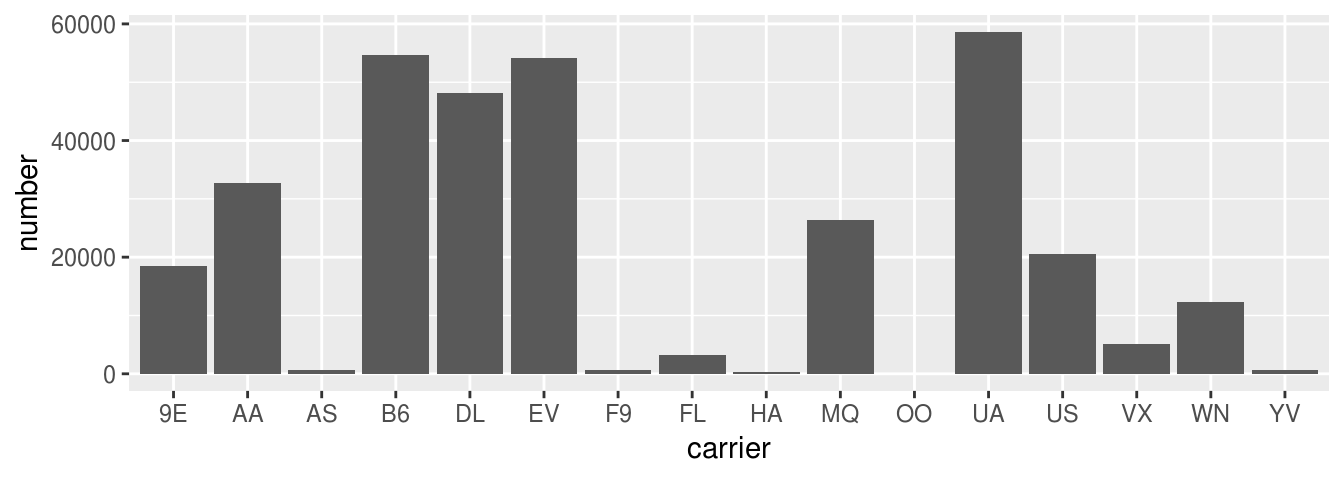
\includegraphics[width=\textwidth]{ismaykim_files/figure-latex/flightscol-1} 

}

\caption{Number of flights departing NYC in 2013 by airline using
geom\_col}\label{fig:flightscol}
\end{figure}

\begin{learncheck}
\textbf{\emph{Learning check}}
\end{learncheck}

\textbf{(LC3.26)} Why are histograms inappropriate for visualizing
categorical variables?

\textbf{(LC3.27)} What is the difference between histograms and
barplots?

\textbf{(LC3.28)} How many Envoy Air flights departed NYC in 2013?

\textbf{(LC3.29)} What was the seventh highest airline in terms of
departed flights from NYC in 2013? How could we better present the table
to get this answer quickly?

\begin{learncheck}

\end{learncheck}

\subsection{Must avoid pie charts!}\label{must-avoid-pie-charts}

Unfortunately, one of the most common plots seen today for categorical
data is the pie chart. While they may see harmless enough, they actually
present a problem in that humans are unable to judge angles well. As
Naomi Robbins describes in her book ``Creating More Effective Graphs''
\citep{robbins2013}, we overestimate angles greater than 90 degrees and
we underestimate angles less than 90 degrees. In other words, it is
difficult for us to determine relative size of one piece of the pie
compared to another.

Let's examine our previous barplot example on the number of flights
departing NYC by airline. This time we will use a pie chart. As you
review this chart, try to identify

\begin{itemize}
\tightlist
\item
  how much larger the portion of the pie is for ExpressJet Airlines
  (\texttt{EV}) compared to US Airways (\texttt{US}),
\item
  what the third largest carrier is in terms of departing flights, and
\item
  how many carriers have fewer flights than United Airlines
  (\texttt{UA})?
\end{itemize}

\begin{figure}

{\centering 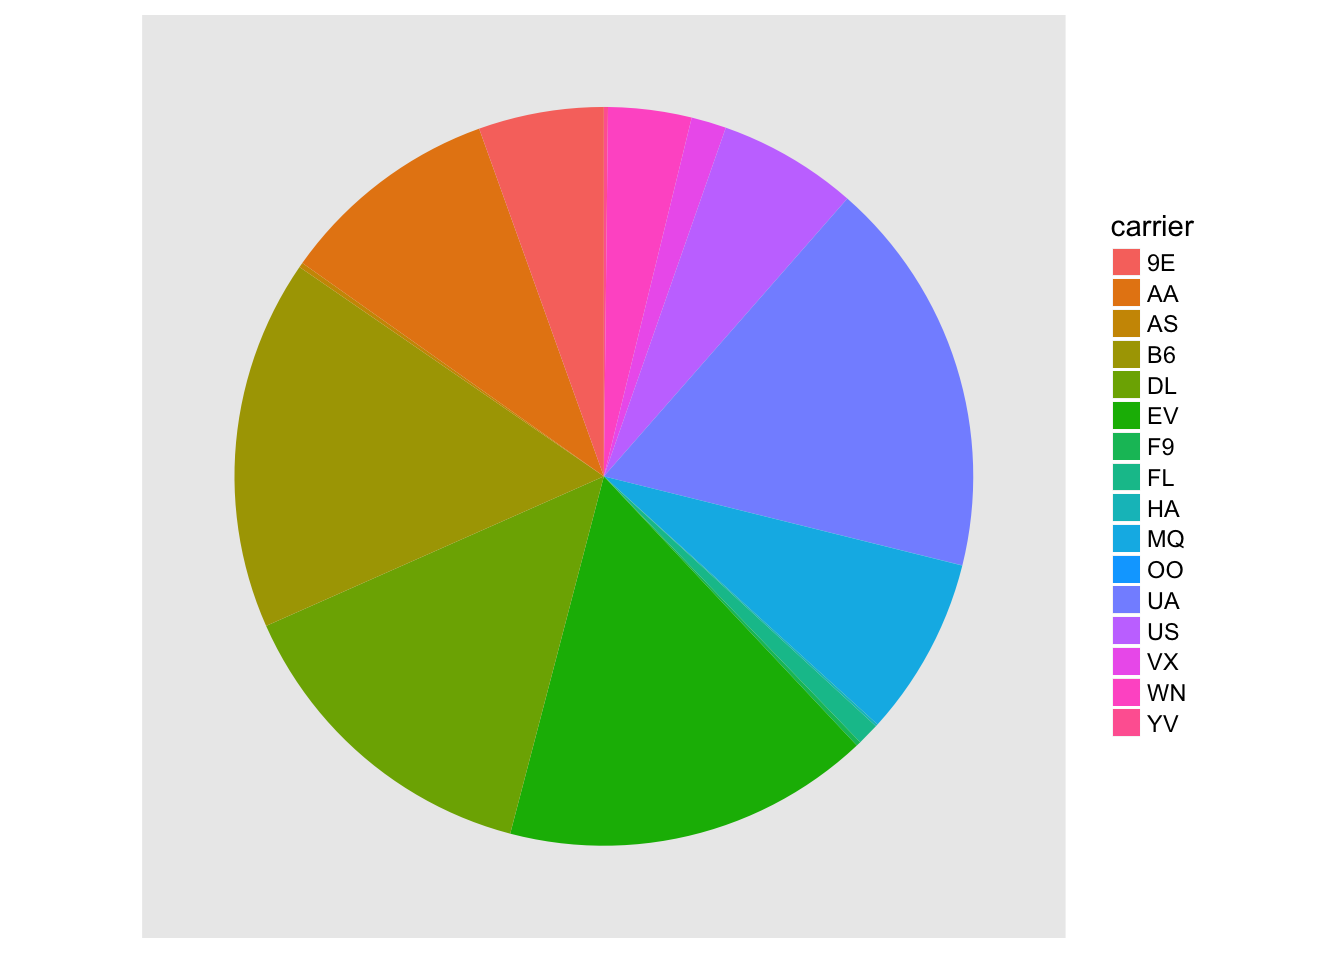
\includegraphics[width=\textwidth]{ismaykim_files/figure-latex/carrierpie-1} 

}

\caption{The dreaded pie chart}\label{fig:carrierpie}
\end{figure}

While it is quite easy to look back at the barplot to get the answer to
these questions, it's quite difficult to get the answers correct when
looking at the pie graph. Barplots can always present the information in
a way that is easier for the eye to determine relative position. There
may be one exception from Nathan Yau at
\href{https://flowingdata.com/2008/09/19/pie-i-have-eaten-and-pie-i-have-not-eaten/}{FlowingData.com}
but we will leave this for the reader to decide:

\begin{figure}

{\centering 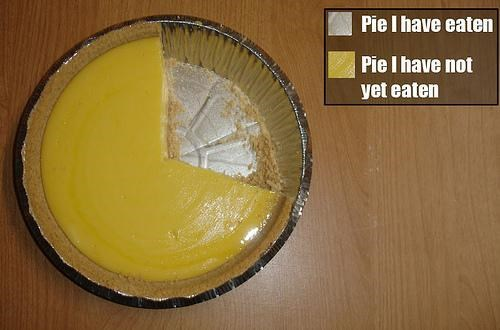
\includegraphics[width=\textwidth,height=2.5in]{images/Pie-I-have-Eaten} 

}

\caption{The only good pie chart}\label{fig:unnamed-chunk-49}
\end{figure}

\begin{learncheck}
\textbf{\emph{Learning check}}
\end{learncheck}

\textbf{(LC3.30)} Why should pie charts be avoided and replaced by
barplots?

\textbf{(LC3.31)} What is your opinion as to why pie charts continue to
be used?

\begin{learncheck}

\end{learncheck}

\subsection{Using barplots to compare two categorical
variables}\label{using-barplots-to-compare-two-categorical-variables}

Barplots are the go-to way to visualize the frequency of different
categories of a categorical variable. They make it easy to order the
counts and to compare the frequencies of one group to another. Another
use of barplots (unfortunately, sometimes inappropriately and
confusingly) is to compare two categorical variables together. Let's
examine the distribution of outgoing flights from NYC by
\texttt{carrier} and \texttt{airport}.

We begin by getting the names of the airports in NYC that were included
in the \texttt{flights} data-set. Here, we preview the
\texttt{inner\_join()} function from Chapter \ref{wrangling}. This
function will join the data frame \texttt{flights} with the data frame
\texttt{airports} by matching rows that have the same airport code.
However, in \texttt{flights} the airport code is included in the
\texttt{origin} variable whereas in \texttt{airports} the airport code
is included in the \texttt{faa} variable. We will revisit such examples
in Section \ref{joins} on joining data-sets.

\begin{Shaded}
\begin{Highlighting}[]
\NormalTok{flights_namedports <-}\StringTok{ }\NormalTok{flights }\OperatorTok\StringTok{ }
\StringTok{  }\KeywordTok{inner_join}\NormalTok{(airports, }\DataTypeTok{by =} \KeywordTok{c}\NormalTok{(}\StringTok{"origin"}\NormalTok{ =}\StringTok{ "faa"}\NormalTok{))}
\end{Highlighting}
\end{Shaded}

After running \texttt{View(flights\_namedports)}, we see that
\texttt{name} now corresponds to the name of the airport as referenced
by the \texttt{origin} variable. We will now plot \texttt{carrier} as
the horizontal variable. When we specify \texttt{geom\_bar}, it will
specify \texttt{count} as being the vertical variable. A new addition
here is \texttt{fill\ =\ name}. Look over what was produced from the
plot to get an idea of what this argument gives.

\begin{Shaded}
\begin{Highlighting}[]
\KeywordTok{ggplot}\NormalTok{(}\DataTypeTok{data =}\NormalTok{ flights_namedports, }
       \DataTypeTok{mapping =} \KeywordTok{aes}\NormalTok{(}\DataTypeTok{x =}\NormalTok{ carrier, }\DataTypeTok{fill =}\NormalTok{ name)) }\OperatorTok{+}
\StringTok{  }\KeywordTok{geom_bar}\NormalTok{()}
\end{Highlighting}
\end{Shaded}

\begin{figure}

{\centering \includegraphics[width=\textwidth]{ismaykim_files/figure-latex/unnamed-chunk-52-1} 

}

\caption{Stacked barplot comparing the number of flights by carrier and airport}\label{fig:unnamed-chunk-52}
\end{figure}

This plot is what is known as a \emph{stacked barplot}. While simple to
make, it often leads to many problems. For example in this plot, it is
difficult to compare the heights of the different colors (corresponding
to the number of flights from each airport) between the bars
(corresponding to the different carriers).

Note that \texttt{fill} is an \texttt{aes}thetic just like \texttt{x} is
an \texttt{aes}thetic, and thus must be included within the parentheses
of the \texttt{aes()} mapping. The following code, where the
\texttt{fill} \texttt{aes}thetic is specified on the outside will yield
an error. This is a fairly common error that new \texttt{ggplot} users
make:

\begin{Shaded}
\begin{Highlighting}[]
\KeywordTok{ggplot}\NormalTok{(}\DataTypeTok{data =}\NormalTok{ flights_namedports, }
       \DataTypeTok{mapping =} \KeywordTok{aes}\NormalTok{(}\DataTypeTok{x =}\NormalTok{ carrier), }\DataTypeTok{fill =}\NormalTok{ name) }\OperatorTok{+}
\StringTok{  }\KeywordTok{geom_bar}\NormalTok{()}
\end{Highlighting}
\end{Shaded}

\begin{learncheck}
\textbf{\emph{Learning check}}
\end{learncheck}

\textbf{(LC3.32)} What kinds of questions are not easily answered by
looking at the above figure?

\textbf{(LC3.33)} What can you say, if anything, about the relationship
between airline and airport in NYC in 2013 in regards to the number of
departing flights?

\begin{learncheck}

\end{learncheck}

Another variation on the stacked barplot is the \emph{side-by-side
barplot} also called a \emph{dodged barplot}.

\begin{Shaded}
\begin{Highlighting}[]
\KeywordTok{ggplot}\NormalTok{(}\DataTypeTok{data =}\NormalTok{ flights_namedports, }
       \DataTypeTok{mapping =} \KeywordTok{aes}\NormalTok{(}\DataTypeTok{x =}\NormalTok{ carrier, }\DataTypeTok{fill =}\NormalTok{ name)) }\OperatorTok{+}
\StringTok{  }\KeywordTok{geom_bar}\NormalTok{(}\DataTypeTok{position =} \StringTok{"dodge"}\NormalTok{)}
\end{Highlighting}
\end{Shaded}

\begin{figure}

{\centering \includegraphics[width=\textwidth]{ismaykim_files/figure-latex/unnamed-chunk-55-1} 

}

\caption{Side-by-side AKA dodged barplot comparing the number of flights by carrier and airport}\label{fig:unnamed-chunk-55}
\end{figure}

\begin{learncheck}
\textbf{\emph{Learning check}}
\end{learncheck}

\textbf{(LC3.34)} Why might the side-by-side (AKA dodged) barplot be
preferable to a stacked barplot in this case?

\textbf{(LC3.35)} What are the disadvantages of using a side-by-side
(AKA dodged) barplot, in general?

\begin{learncheck}

\end{learncheck}

Lastly, an often preferred type of barplot is the \emph{faceted
barplot}. We already saw this concept of faceting and small multiples in
Section \ref{facets}. This gives us a nicer way to compare the
distributions across both \texttt{carrier} and airport/\texttt{name}.

\begin{Shaded}
\begin{Highlighting}[]
\KeywordTok{ggplot}\NormalTok{(}\DataTypeTok{data =}\NormalTok{ flights_namedports, }
       \DataTypeTok{mapping =} \KeywordTok{aes}\NormalTok{(}\DataTypeTok{x =}\NormalTok{ carrier, }\DataTypeTok{fill =}\NormalTok{ name)) }\OperatorTok{+}
\StringTok{  }\KeywordTok{geom_bar}\NormalTok{() }\OperatorTok{+}
\StringTok{  }\KeywordTok{facet_wrap}\NormalTok{(}\OperatorTok{~}\StringTok{ }\NormalTok{name, }\DataTypeTok{ncol =} \DecValTok{1}\NormalTok{)}
\end{Highlighting}
\end{Shaded}

\begin{figure}

{\centering \includegraphics[width=\textwidth]{ismaykim_files/figure-latex/facet-bar-vert-1} 

}

\caption{Faceted barplot comparing the number of flights by carrier and airport}\label{fig:facet-bar-vert}
\end{figure}

\begin{learncheck}
\textbf{\emph{Learning check}}
\end{learncheck}

\textbf{(LC3.36)} Why is the faceted barplot preferred to the
side-by-side and stacked barplots in this case?

\textbf{(LC3.37)} What information about the different carriers at
different airports is more easily seen in the faceted barplot?

\begin{learncheck}

\end{learncheck}

\subsection{Summary}\label{summary-4}

Barplots are the preferred way of displaying categorical variables. They
are easy-to-understand and make it easy to compare across groups of a
categorical variable. When dealing with more than one categorical
variable, faceted barplots are frequently preferred over side-by-side or
stacked barplots. Stacked barplots are sometimes nice to look at, but it
is quite difficult to compare across the levels since the sizes of the
bars are all of different sizes. Side-by-side barplots can provide an
improvement on this, but the issue about comparing across groups still
must be dealt with.

\section{Conclusion}\label{conclusion-1}

\subsection{Putting it all together}\label{putting-it-all-together}

Let's recap all five of the Five Named Graphs (5NG) in Table
\ref{tab:viz-summary-table} summarizing their differences. Using these
5NG, you'll be able to visualize the distributions and relationships of
variables contained in a wide array of datasets. This will be even more
the case as we start to map more variables to more of each
\texttt{geom}etric object's \texttt{aes}thetic attribute options,
further unlocking the awesome power of the \texttt{ggplot2} package.

\begin{table}

\caption{\label{tab:viz-summary-table}Summary of 5NG}
\centering
\fontsize{10}{12}\selectfont
\begin{tabular}[t]{rllll}
\toprule
  & Named graph & Shows & Geometric object & Notes\\
\midrule
1 & Scatterplot & Relationship between \textbackslash{}n 2 numerical variables & `geom\_point()` & \\
2 & Linegraph & Relationship between \textbackslash{}n 2 numerical variables & `geom\_line()` & Used when there is a sequential order to x-variable e.g. time\\
3 & Histogram & Distribution of \textbackslash{}n 1 numerical variable & `geom\_histogram()` & Facetted histogram shows distribution of 1 numerical variable split by 1 categorical variable\\
4 & Boxplot & Distribution of \textbackslash{}n 1 numerical variable split \textbackslash{}n by 1 categorical variable & `geom\_boxplot()` & \\
5 & Barplot & Distribution of \textbackslash{}n 1 categorical variable & `geom\_barplot()` when counts are not pre-counted & Stacked \& dodged barplots show distribution of 2 categorical variables\\
 &  &  & `geom\_col()` when counts are pre-counted & \\
\bottomrule
\end{tabular}
\end{table}

\subsection{Review questions}\label{review-questions}

Review questions have been designed using the
\href{https://rudeboybert.github.io/fivethirtyeight/}{\texttt{fivethirtyeight}
R package} \citep{R-fivethirtyeight} with links to the corresponding
FiveThirtyEight.com articles in our free DataCamp course
\textbf{Effective Data Storytelling using the \texttt{tidyverse}}. The
material in this chapter is covered in the chapters of the DataCamp
course available below:

\begin{itemize}
\tightlist
\item
  \href{https://campus.datacamp.com/courses/effective-data-storytelling-using-the-tidyverse-free/17581?ex=1}{Scatterplots
  \& Linegraphs}
\item
  \href{https://campus.datacamp.com/courses/effective-data-storytelling-using-the-tidyverse-free/17582?ex=1}{Histograms
  \& Boxplots}
\item
  \href{https://campus.datacamp.com/courses/effective-data-storytelling-using-the-tidyverse-free/17583?ex=1}{Barplots}
\item
  \href{https://campus.datacamp.com/courses/effective-data-storytelling-using-the-tidyverse-free/17584?ex=1}{ggplot2
  Review}
\end{itemize}

\subsection{What's to come?}\label{whats-to-come-1}

In Chapter \ref{tidy}, we'll introduce the concept of ``tidy data'' and
how it is used as a key data format for all the packages we use in this
textbook. You'll see that the concept appears to be simple, but actually
can be a little challenging to decipher without careful practice. We'll
also investigate how to import CSV (comma-separated value) files into R
using the \texttt{readr} package.

\subsection{Resources}\label{resources}

An excellent resource as you begin to create plots using the
\texttt{ggplot2} package is a cheatsheet that RStudio has put together
entitled ``Data Visualization with ggplot2'' available

\begin{itemize}
\tightlist
\item
  by clicking
  \href{https://www.rstudio.com/wp-content/uploads/2016/11/ggplot2-cheatsheet-2.1.pdf}{here}
  or
\item
  by clicking the RStudio Menu Bar -\textgreater{} Help -\textgreater{}
  Cheatsheets -\textgreater{} ``Data Visualization with
  \texttt{ggplot2}''
\end{itemize}

This cheatsheet covers more than what we've discussed in this chapter
but provides nice visual descriptions of what each function produces.

\subsection{Script of R code}\label{script-of-r-code}

An R script file of all R code used in this chapter is available
\href{scripts/03-visualization.R}{here}.

\chapter{Tidy Data via tidyr}\label{tidy}

In Subsection \ref{programming-concepts} we introduced the concept of a
data frame: a rectangular spreadsheet-like representation of data in R
where the rows correspond to observations and the columns correspond to
variables describing each observation. In Section \ref{nycflights13}, we
started explorations of our first data frame \texttt{flights} included
in the \texttt{nycflights13} package. In Chapter \ref{viz} we made
graphics using data contained in \texttt{flights} and other data frames.

In this chapter, we extend some of these ideas by discussing a type of
data formatting called ``tidy'' data. You will see that having data
stored in ``tidy'' format is about more than what the colloquial
definition of the term ``tidy'' might suggest of having your data
``neatly organized'' in a spreadsheet. Instead, we define the term
``tidy'' in a more rigorous fashion, outlining a set of rules by which
data can be stored and the implications of these rules on analyses.

Although knowledge of this type of data formatting was not necessary in
our treatment of data visualization in Chapter \ref{viz} since all the
data was already in tidy format, we'll see going forward that having
tidy data will allow you to more easily create data visualizations in a
wide range of settings. Furthermore, it will also help you with data
wrangling in Chapter \ref{wrangling} and in all subsequent chapters in
this book when we cover regression and discuss statistical inference.

\subsection*{Needed packages}\label{needed-packages-1}


Let's load all the packages needed for this chapter (this assumes you've
already installed them). If needed, read Section \ref{packages} for
information on how to install and load R packages.

\begin{Shaded}
\begin{Highlighting}[]
\KeywordTok{library}\NormalTok{(dplyr)}
\KeywordTok{library}\NormalTok{(ggplot2)}
\KeywordTok{library}\NormalTok{(nycflights13)}
\KeywordTok{library}\NormalTok{(tidyr)}
\KeywordTok{library}\NormalTok{(readr)}
\end{Highlighting}
\end{Shaded}

\subsection*{DataCamp}\label{datacamp-1}


Our approach to introducing the concept of ``tidy'' data is aligned with
the approach taken in \href{https://twitter.com/apreshill}{Alison
Hill's} DataCamp course ``Working with Data in the Tidyverse,'' a course
where students learn to work with data using tools from the tidyverse in
R. If you're interested in complementing your learning below in an
interactive online environment, click on the image below to access the
course. The relevant chapter is Chapter 3 ``Tidy your data.''

\begin{center}
\href{https://www.datacamp.com/courses/working-with-data-in-the-tidyverse}{\includegraphics[width=0.5\textwidth]{images/datacamp_working_with_data.png}}
\end{center}

\begin{center}\rule{0.5\linewidth}{\linethickness}\end{center}

\section{What is tidy data?}\label{what-is-tidy-data}

You have surely heard the word ``tidy'' in your life:

\begin{itemize}
\tightlist
\item
  ``Tidy up your room!''
\item
  ``Please write your homework in a tidy way so that it is easier to
  grade and to provide feedback.''
\item
  Marie Kondo's best-selling book
  \href{https://www.amazon.com/Life-Changing-Magic-Tidying-Decluttering-Organizing/dp/1607747308/ref=sr_1_1?ie=UTF8\&qid=1469400636\&sr=8-1\&keywords=tidying+up}{\emph{The
  Life-Changing Magic of Tidying Up: The Japanese Art of Decluttering
  and Organizing}}
\item
  ``I am not by any stretch of the imagination a tidy person, and the
  piles of unread books on the coffee table and by my bed have a
  plaintive, pleading quality to me - `Read me, please!'\,'' - Linda
  Grant
\end{itemize}

What does it mean for your data to be ``tidy''? Beyond just being
organized, in the context of this book having ``tidy'' data means that
your data follows a standardized format. This makes it easier for you
and others to visualize your data, to wrangle/transform your data, and
to model your data. We will follow Hadley Wickham's definition of
\emph{tidy data} here \citep{tidy}:

\begin{quote}
A dataset is a collection of values, usually either numbers (if
quantitative) or strings AKA text data (if qualitative). Values are
organised in two ways. Every value belongs to a variable and an
observation. A variable contains all values that measure the same
underlying attribute (like height, temperature, duration) across units.
An observation contains all values measured on the same unit (like a
person, or a day, or a city) across attributes.
\end{quote}

\begin{quote}
Tidy data is a standard way of mapping the meaning of a dataset to its
structure. A dataset is messy or tidy depending on how rows, columns and
tables are matched up with observations, variables and types. In
\emph{tidy data}:
\end{quote}

\begin{quote}
\begin{enumerate}
\def\labelenumi{\arabic{enumi}.}
\tightlist
\item
  Each variable forms a column.
\item
  Each observation forms a row.
\item
  Each type of observational unit forms a table.
\end{enumerate}
\end{quote}

\begin{figure}

{\centering \includegraphics[width=\textwidth]{images/tidy-1} 

}

\caption{Tidy data graphic from http://r4ds.had.co.nz/tidy-data.html}\label{fig:tidyfig}
\end{figure}

For example, say the following table consists of stock prices:

\begin{table}

\caption{\label{tab:unnamed-chunk-60}Stock Prices (Non-Tidy Format)}
\centering
\fontsize{10}{12}\selectfont
\begin{tabular}[t]{llll}
\toprule
Date & Boeing Stock Price & Amazon Stock Price & Google Stock Price\\
\midrule
2009-01-01 & \$173.55 & \$174.90 & \$174.34\\
2009-01-02 & \$172.61 & \$171.42 & \$170.04\\
\bottomrule
\end{tabular}
\end{table}

Although the data are neatly organized in a spreadsheet-type format,
they are not in tidy format since there are three variables
corresponding to three unique pieces of information (Date, Stock Name,
and Stock Price), but there are not three columns. In tidy data format
each variable should be its own column, as shown below. Notice that both
tables present the same information, but in different formats.

\begin{table}

\caption{\label{tab:unnamed-chunk-61}Stock Prices (Tidy Format)}
\centering
\fontsize{10}{12}\selectfont
\begin{tabular}[t]{lll}
\toprule
Date & Stock Name & Stock Price\\
\midrule
2009-01-01 & Boeing & \$173.55\\
2009-01-02 & Boeing & \$172.61\\
2009-01-01 & Amazon & \$174.90\\
2009-01-02 & Amazon & \$171.42\\
2009-01-01 & Google & \$174.34\\
2009-01-02 & Google & \$170.04\\
\bottomrule
\end{tabular}
\end{table}

However, consider the following table

\begin{table}

\caption{\label{tab:unnamed-chunk-62}Date, Boeing Price, Weather Data}
\centering
\fontsize{10}{12}\selectfont
\begin{tabular}[t]{lll}
\toprule
Date & Boeing Price & Weather\\
\midrule
2009-01-01 & \$173.55 & Sunny\\
2009-01-02 & \$172.61 & Overcast\\
\bottomrule
\end{tabular}
\end{table}

In this case, even though the variable ``Boeing Price'' occurs again,
the data \emph{is} tidy since there are three variables corresponding to
three unique pieces of information (Date, Boeing stock price, and the
weather that particular day).

The non-tidy data format in the original table is also known as
\href{https://en.wikipedia.org/wiki/Wide_and_narrow_data}{``wide''}
format whereas the tidy data format in the second table is also known as
\href{https://en.wikipedia.org/wiki/Wide_and_narrow_data\#Narrow}{``long/narrow''}
data format.

In this book, we will work mostly with datasets that are already in tidy
format even though a lot of the world's data isn't always in this nice
format that the \texttt{tidyverse} gets its name from. Data that is in
wide format can be converted to ``tidy'' format by using the
\texttt{gather()} function in the \texttt{tidyr} package \citep{R-tidyr}
in the \texttt{tidyverse}; we'll show an example of this in Section
\ref{tidying}. For other examples of converting a dataset into ``tidy''
format, check out the different functions available for data tidying and
a case study using data from the World Health Organization in
\href{http://r4ds.had.co.nz/tidy-data.html}{R for Data Science}
\citep{rds2016}.

\begin{learncheck}
\textbf{\emph{Learning check}}
\end{learncheck}

\textbf{(LC4.1)} Consider the following data frame of average number of
servings of beer, spirits, and wine consumption in three countries as
reported in the FiveThirtyEight article
\href{https://fivethirtyeight.com/features/dear-mona-followup-where-do-people-drink-the-most-beer-wine-and-spirits/}{Dear
Mona Followup: Where Do People Drink The Most Beer, Wine And Spirits?}

\begin{verbatim}
# A tibble: 3 x 4
  country     beer_servings spirit_servings wine_servings
  <chr>               <int>           <int>         <int>
1 Canada                240             122           100
2 South Korea           140              16             9
3 USA                   249             158            84
\end{verbatim}

This data frame is not in tidy format. What would it look like if it
were?

\begin{learncheck}

\end{learncheck}

\begin{center}\rule{0.5\linewidth}{\linethickness}\end{center}

\section{Back to nycflights13}\label{back-to-nycflights13}

Recall the \texttt{nycflights13} package with data about all domestic
flights departing from New York City in 2013 that we introduced in
Section \ref{nycflights13} and used extensively in Chapter \ref{viz} to
create visualizations. In particular, let's revisit the \texttt{flights}
data frame by running \texttt{View(flights)} in your console. We see
that \texttt{flights} has a rectangular shape with each row
corresponding to a different flight and each column corresponding to a
characteristic of that flight. This matches exactly with how Hadley
Wickham defined tidy data:

\begin{enumerate}
\def\labelenumi{\arabic{enumi}.}
\tightlist
\item
  Each variable forms a column.
\item
  Each observation forms a row.
\end{enumerate}

But what about the third property?

\begin{quote}
\begin{enumerate}
\def\labelenumi{\arabic{enumi}.}
\setcounter{enumi}{2}
\tightlist
\item
  Each type of observational unit forms a table.
\end{enumerate}
\end{quote}

\subsection{Observational units}\label{observational-units}

We identified earlier that the observational unit in the
\texttt{flights} dataset is an individual flight. And we have shown that
this dataset consists of 336,776 flights with 19 variables. In other
words, rows of this dataset don't refer to a measurement on an airline
or on an airport; they refer to characteristics/measurements on a given
flight from New York City in 2013.

Also included in the \texttt{nycflights13} package are datasets with
different observational units \citep{R-nycflights13}:

\begin{itemize}
\tightlist
\item
  \texttt{airlines}: translation between two letter IATA carrier codes
  and names (16 in total)
\item
  \texttt{planes}: construction information about each of 3,322 planes
  used
\item
  \texttt{weather}: hourly meteorological data (about 8705 observations)
  for each of the three NYC airports
\item
  \texttt{airports}: airport names and locations
\end{itemize}

The organization of this data follows the third ``tidy'' data property:
observations corresponding to the same observational unit should be
saved in the same table/data frame.

Another example involves a spreadsheet of all students enrolled in a
university along with information about them, such as name, gender, and
date of birth. Each row represents an individual student, which is the
observational unit in question.

\subsection{Identification vs measurement
variables}\label{identification-vs-measurement}

There is a subtle difference between the kinds of variables that you
will encounter in data frames: \emph{measurement variables} and
\emph{identification variables}. The \texttt{airports} data frame you
worked with above contains both these types of variables. Recall that in
\texttt{airports} the observational unit is an airport, and thus each
row corresponds to one particular airport. Let's pull them apart using
the \texttt{glimpse} function:

\begin{Shaded}
\begin{Highlighting}[]
\KeywordTok{glimpse}\NormalTok{(airports)}
\end{Highlighting}
\end{Shaded}

\begin{verbatim}
Observations: 1,458
Variables: 8
$ faa   <chr> "04G", "06A", "06C", "06N", "09J", "0A9", "0G6...
$ name  <chr> "Lansdowne Airport", "Moton Field Municipal Ai...
$ lat   <dbl> 41.13047, 32.46057, 41.98934, 41.43191, 31.074...
$ lon   <dbl> -80.61958, -85.68003, -88.10124, -74.39156, -8...
$ alt   <int> 1044, 264, 801, 523, 11, 1593, 730, 492, 1000,...
$ tz    <dbl> -5, -6, -6, -5, -5, -5, -5, -5, -5, -8, -5, -6...
$ dst   <chr> "A", "A", "A", "A", "A", "A", "A", "A", "U", "...
$ tzone <chr> "America/New_York", "America/Chicago", "Americ...
\end{verbatim}

The variables \texttt{faa} and \texttt{name} are what we will call
\emph{identification variables}: variables that uniquely identify each
observational unit. They are mainly used to provide a unique name to
each observational unit, thereby allowing us to uniquely identify them.
\texttt{faa} gives the unique code provided by the FAA for that airport,
while the \texttt{name} variable gives the longer more natural name of
the airport. The remaining variables (\texttt{lat}, \texttt{lon},
\texttt{alt}, \texttt{tz}, \texttt{dst}, \texttt{tzone}) are often
called \emph{measurement} or \emph{characteristic} variables: variables
that describe properties of each observational unit, in other words each
observation in each row. For example, \texttt{lat} and \texttt{long}
describe the latitude and longitude of each airport.

So in our above example of a spreadsheet of all students enrolled at a
university, email address could be treated as an identical variable
since it uniquely identifies each observational unit i.e.~each student,
while date of birth could not since it is possible (and highly probable)
that two students share the same birthday.

Furthermore, sometimes a single variable might not be enough to uniquely
identify each observational unit: combinations of variables might be
needed (see Learning Check below). While it is not an absolute rule, for
organizational purposes it is considered good practice to have your
identification variables in the far left-most columns of your data
frame.

\begin{learncheck}
\textbf{\emph{Learning check}}
\end{learncheck}

\textbf{(LC4.2)} What properties of the observational unit do each of
\texttt{lat}, \texttt{lon}, \texttt{alt}, \texttt{tz}, \texttt{dst}, and
\texttt{tzone} describe for the \texttt{airports} data frame? Note that
you may want to use \texttt{?airports} to get more information.

\textbf{(LC4.3)} Provide the names of variables in a data frame with at
least three variables in which one of them is an identification variable
and the other two are not. In other words, create your own tidy dataset
that matches these conditions.

\begin{learncheck}

\end{learncheck}

\begin{center}\rule{0.5\linewidth}{\linethickness}\end{center}

\section{Importing spreadsheets into R}\label{csv}

Up to this point, we've used data either stored inside of an R package
or we've manually created the data such as the \texttt{fruits} and
\texttt{fruits\_counted} data in Subsection \ref{geombar}. Another
common way to get data into R is by reading in data from a spreadsheet
file either on your computer or online. Spreadsheet data is often saved
in one of two formats:

\begin{itemize}
\tightlist
\item
  A \emph{Comma Separated Values} \texttt{.csv} file. You can think of a
  CSV file as a bare-bones spreadsheet where:

  \begin{itemize}
  \tightlist
  \item
    Each line in the file corresponds to one row of data/one
    observation.
  \item
    Values for each line are separated with commas. In other words, the
    values of different variables are separated by commas.
  \item
    The first line is often, but not always, a \emph{header} row
    indicating the names of the columns/variables.
  \end{itemize}
\item
  An Excel \texttt{.xlsx} file. This format is based on Microsoft's
  proprietary Excel software. As opposed to a bare-bones \texttt{.csv}
  files, \texttt{.xlsx} Excel files contain a lot of \emph{metadata}, or
  put more simply, data about the data. Examples include the use of bold
  and italic fonts, colored cells, different column widths, and formula
  macros etc.
\end{itemize}

\href{https://www.google.com/sheets/about/}{Google Sheets} allows you to
download your data in both comma separated values \texttt{.csv} and
Excel \texttt{.xlsx} formats: Go to the Google Sheets menu bar
-\textgreater{} File -\textgreater{} Download as -\textgreater{} Select
``Microsoft Excel'' or ``Comma-separated values.''

We'll cover two methods for importing data in R: one using the R console
and the other using RStudio's graphical interface.

\subsection{Method 1: From the console}\label{method-1-from-the-console}

First, let's download a \emph{Comma Separated Values} (CSV) file of
ratings of the level of democracy in different countries spanning 1952
to 1992: \url{https://moderndive.com/data/dem_score.csv}. We use the
\texttt{read\_csv()} function from the \texttt{readr} package to read it
off the web and then take a look.

\begin{Shaded}
\begin{Highlighting}[]
\KeywordTok{library}\NormalTok{(readr)}
\NormalTok{dem_score <-}\StringTok{ }\KeywordTok{read_csv}\NormalTok{(}\StringTok{"https://moderndive.com/data/dem_score.csv"}\NormalTok{)}
\NormalTok{dem_score}
\end{Highlighting}
\end{Shaded}

\begin{verbatim}
# A tibble: 96 x 10
   country `1952` `1957` `1962` `1967` `1972` `1977` `1982`
   <chr>    <int>  <int>  <int>  <int>  <int>  <int>  <int>
 1 Albania     -9     -9     -9     -9     -9     -9     -9
 2 Argent~     -9     -1     -1     -9     -9     -9     -8
 3 Armenia     -9     -7     -7     -7     -7     -7     -7
 4 Austra~     10     10     10     10     10     10     10
 5 Austria     10     10     10     10     10     10     10
 6 Azerba~     -9     -7     -7     -7     -7     -7     -7
 7 Belarus     -9     -7     -7     -7     -7     -7     -7
 8 Belgium     10     10     10     10     10     10     10
 9 Bhutan     -10    -10    -10    -10    -10    -10    -10
10 Bolivia     -4     -3     -3     -4     -7     -7      8
# ... with 86 more rows, and 2 more variables: `1987` <int>,
#   `1992` <int>
\end{verbatim}

In this \texttt{dem\_score} data frame, the minimum value of -10
corresponds to a highly autocratic nation whereas a value of 10
corresponds to a highly democratic nation.

\subsection{Method 2: Using RStudio's
interface}\label{method-2-using-rstudios-interface}

Let's read in the same data saved in Excel format this time at
\url{https://moderndive.com/data/dem_score.xlsx}, but using RStudio's
graphical interface instead of via the R console. First download the
Excel file, then go to the Files pane of RStudio -\textgreater{}
Navigate to the directory where your downloaded \texttt{dem\_score.xlsx}
is saved -\textgreater{} Click on \texttt{dem\_score.xlsx}
-\textgreater{} Click ``Import Dataset\ldots{}'' -\textgreater{} Click
``Import Dataset\ldots{}'' At this point you should see an image like in

\begin{figure}
\centering
\includegraphics{images/read_excel.png}
\caption{}
\end{figure}

After clicking on the ``Import'' button on the bottom right RStudio save
this spreadsheet's data in a data frame called \texttt{dem\_score} and
display its contents in the spreadsheet viewer. Furthermore you'll see
the code that read in your data in the console; you can copy and paste
this code to reload your data again later instead of repeating the above
manual process.

\begin{center}\rule{0.5\linewidth}{\linethickness}\end{center}

\section{\texorpdfstring{Converting to ``tidy'' data
format}{Converting to tidy data format}}\label{tidying}

In this Section, we'll show you how to convert a dataset that isn't in
``tidy'' format i.e. ``wide'' format, to a dataset that is in ``tidy''
format i.e. ``long/narrow'' format. Let's use the \texttt{dem\_score}
data frame we loaded from a spreadsheet in the previous Section but
focus on only data corresponding to the country of Guatemala.

\begin{Shaded}
\begin{Highlighting}[]
\NormalTok{guat_dem <-}\StringTok{ }\NormalTok{dem_score }\OperatorTok\StringTok{ }
\StringTok{  }\KeywordTok{filter}\NormalTok{(country }\OperatorTok{==}\StringTok{ "Guatemala"}\NormalTok{)}
\NormalTok{guat_dem}
\end{Highlighting}
\end{Shaded}

\begin{verbatim}
# A tibble: 1 x 10
  country `1952` `1957` `1962` `1967` `1972` `1977` `1982` `1987`
  <chr>    <int>  <int>  <int>  <int>  <int>  <int>  <int>  <int>
1 Guatem~      2     -6     -5      3      1     -3     -7      3
# ... with 1 more variable: `1992` <int>
\end{verbatim}

Now let's produce a plot showing how the democracy scores have changed
over the 40 years from 1952 to 1992 for Guatemala. Let's start by laying
out how we would map our aesthetics to variables in the data frame:

\begin{itemize}
\tightlist
\item
  The \texttt{data} frame is \texttt{guat\_dem} by setting
  \texttt{data\ =\ guat\_dem}
\end{itemize}

What are the names of the variables to plot? We'd like to see how the
democracy score has changed over the years. Now we are stuck in a
predicament. We see that we have a variable named \texttt{country} but
its only value is \texttt{"Guatemala"}. We have other variables denoted
by different year values. Unfortunately, we've run into a dataset that
is not in the appropriate format to apply the Grammar of Graphics and
\texttt{ggplot2}. Remember that \texttt{ggplot2} is a package in the
\texttt{tidyverse} and, thus, needs data to be in a tidy format. We'd
like to finish off our mapping of aesthetics to variables by doing
something like

\begin{itemize}
\tightlist
\item
  The \texttt{aes}thetic mapping is set by
  \texttt{aes(x\ =\ year,\ y\ =\ democracy\_score)}
\end{itemize}

but this is not possible with our wide-formatted data. We need to take
the values of the current column names in \texttt{guat\_dem} (aside from
\texttt{country}) and convert them into a new variable that will act as
a key called \texttt{year}. Then, we'd like to take the numbers on the
inside of the table and turn them into a column that will act as values
called \texttt{democracy\_score}. Our resulting data frame will have
three columns: \texttt{country}, \texttt{year}, and
\texttt{democracy\_score}.

The \texttt{gather()} function in the \texttt{tidyr} package can
complete this task for us. The first argument to \texttt{gather()}, just
as with \texttt{ggplot2()}, is the \texttt{data} argument where we
specify which data frame we would like to tidy. The next two arguments
to \texttt{gather()} are \texttt{key} and \texttt{value}, which specify
what we'd like to call the new columns that convert our wide data into
long format. Lastly, we include a specification for variables we'd like
to NOT include in this tidying process using a \texttt{-}.

\begin{Shaded}
\begin{Highlighting}[]
\NormalTok{guat_tidy <-}\StringTok{ }\KeywordTok{gather}\NormalTok{(}\DataTypeTok{data =}\NormalTok{ guat_dem, }
                    \DataTypeTok{key =}\NormalTok{ year,}
                    \DataTypeTok{value =}\NormalTok{ democracy_score,}
                    \OperatorTok{-}\StringTok{ }\NormalTok{country) }
\NormalTok{guat_tidy}
\end{Highlighting}
\end{Shaded}

\begin{verbatim}
# A tibble: 9 x 3
  country   year  democracy_score
  <chr>     <chr>           <int>
1 Guatemala 1952                2
2 Guatemala 1957               -6
3 Guatemala 1962               -5
4 Guatemala 1967                3
5 Guatemala 1972                1
6 Guatemala 1977               -3
7 Guatemala 1982               -7
8 Guatemala 1987                3
9 Guatemala 1992                3
\end{verbatim}

We can now create the plot to show how the democracy score of Guatemala
changed from 1952 to 1992 using a linegraph and \texttt{ggplot2}.

\begin{Shaded}
\begin{Highlighting}[]
\KeywordTok{ggplot}\NormalTok{(}\DataTypeTok{data =}\NormalTok{ guat_tidy, }
       \DataTypeTok{mapping =} \KeywordTok{aes}\NormalTok{(}\DataTypeTok{x =}\NormalTok{ year, }\DataTypeTok{y =}\NormalTok{ democracy_score)) }\OperatorTok{+}
\StringTok{  }\KeywordTok{geom_line}\NormalTok{()}
\end{Highlighting}
\end{Shaded}

\begin{verbatim}
geom_path: Each group consists of only one observation. Do you
need to adjust the group aesthetic?
\end{verbatim}

\begin{center}\includegraphics[width=\textwidth]{ismaykim_files/figure-latex/unnamed-chunk-72-1} \end{center}

Observe that the \texttt{year} variable in \texttt{guat\_tidy} is stored
as a character vector since we had to circumvent the naming rules in R
by adding backticks around the different year columns in
\texttt{guat\_dem}. This is leading to \texttt{ggplot} not knowing
exactly how to plot a line using a categorical variable. We can fix this
by using the \texttt{parse\_number()} function in the \texttt{readr}
package and then specify the horizontal axis label to be
\texttt{"year"}:

\begin{Shaded}
\begin{Highlighting}[]
\KeywordTok{ggplot}\NormalTok{(}\DataTypeTok{data =}\NormalTok{ guat_tidy, }
       \DataTypeTok{mapping =} \KeywordTok{aes}\NormalTok{(}\DataTypeTok{x =} \KeywordTok{parse_number}\NormalTok{(year), }
                     \DataTypeTok{y =}\NormalTok{ democracy_score)) }\OperatorTok{+}
\StringTok{  }\KeywordTok{geom_line}\NormalTok{() }\OperatorTok{+}
\StringTok{  }\KeywordTok{labs}\NormalTok{(}\DataTypeTok{x =} \StringTok{"year"}\NormalTok{)}
\end{Highlighting}
\end{Shaded}

\begin{figure}

{\centering \includegraphics[width=\textwidth]{ismaykim_files/figure-latex/guatline-1} 

}

\caption{Guatemala's democracy score ratings from 1952 to 1992}\label{fig:guatline}
\end{figure}

We'll see in Chapter \ref{wrangling} how we could use the
\texttt{mutate()} function to change \texttt{year} to be a numeric
variable instead after we have done our tidying. Notice now that the
mappings of aesthetics to variables make sense in Figure
\ref{fig:guatline}:

\begin{itemize}
\tightlist
\item
  The \texttt{data} frame is \texttt{guat\_tidy} by setting
  \texttt{data\ =\ dem\_score}
\item
  The \texttt{x} \texttt{aes}thetic is mapped to \texttt{year}
\item
  The \texttt{y} \texttt{aes}thetic is mapped to
  \texttt{democracy\_score}
\item
  The \texttt{geom\_}etry chosen is \texttt{line}
\end{itemize}

\begin{learncheck}
\textbf{\emph{Learning check}}
\end{learncheck}

\textbf{(LC4.4)} Convert the \texttt{dem\_score} data frame into a tidy
data frame and assign the name of \texttt{dem\_score\_tidy} to the
resulting long-formatted data frame.

\textbf{(LC4.5)} Read in the life expectancy data stored at
\url{https://moderndive.com/data/le_mess.csv} and convert it to a tidy
data frame.

\begin{learncheck}

\end{learncheck}

\begin{center}\rule{0.5\linewidth}{\linethickness}\end{center}

\section{Optional: Normal forms of
data}\label{optional-normal-forms-of-data}

The datasets included in the \texttt{nycflights13} package are in a form
that minimizes redundancy of data. We will see that there are ways to
\emph{merge} (or \emph{join}) the different tables together easily. We
are capable of doing so because each of the tables have \emph{keys} in
common to relate one to another. This is an important property of
\textbf{normal forms} of data. The process of decomposing data frames
into less redundant tables without losing information is called
\textbf{normalization}. More information is available on
\href{https://en.wikipedia.org/wiki/Database_normalization}{Wikipedia}.

We saw an example of this above with the \texttt{airlines} dataset.
While the \texttt{flights} data frame could also include a column with
the names of the airlines instead of the carrier code, this would be
repetitive since there is a unique mapping of the carrier code to the
name of the airline/carrier.

Below an example is given showing how to \textbf{join} the
\texttt{airlines} data frame together with the \texttt{flights} data
frame by linking together the two datasets via a common \textbf{key} of
\texttt{"carrier"}. Note that this ``joined'' data frame is assigned to
a new data frame called \texttt{joined\_flights}. The \textbf{key}
variable that we frequently join by is one of the \emph{identification
variables} mentioned above.

\begin{Shaded}
\begin{Highlighting}[]
\KeywordTok{library}\NormalTok{(dplyr)}
\NormalTok{joined_flights <-}\StringTok{ }\KeywordTok{inner_join}\NormalTok{(}\DataTypeTok{x =}\NormalTok{ flights, }\DataTypeTok{y =}\NormalTok{ airlines, }\DataTypeTok{by =} \StringTok{"carrier"}\NormalTok{)}
\end{Highlighting}
\end{Shaded}

\begin{Shaded}
\begin{Highlighting}[]
\KeywordTok{View}\NormalTok{(joined_flights)}
\end{Highlighting}
\end{Shaded}

If we \texttt{View} this dataset, we see a new variable has been created
called \texttt{name}. (We will see in Subsection \ref{rename} ways to
change \texttt{name} to a more descriptive variable name.) More
discussion about joining data frames together will be given in Chapter
\ref{wrangling}. We will see there that the names of the columns to be
linked need not match as they did here with \texttt{"carrier"}.

\begin{learncheck}
\textbf{\emph{Learning check}}
\end{learncheck}

\textbf{(LC4.6)} What are common characteristics of ``tidy'' datasets?

\textbf{(LC4.7)} What makes ``tidy'' datasets useful for organizing
data?

\textbf{(LC4.8)} What are some advantages of data in normal forms? What
are some disadvantages?

\begin{learncheck}

\end{learncheck}

\begin{center}\rule{0.5\linewidth}{\linethickness}\end{center}

\section{Conclusion}\label{conclusion-2}

\subsection{Review questions}\label{review-questions-1}

Review questions have been designed using the \texttt{fivethirtyeight} R
package \citep{R-fivethirtyeight} with links to the corresponding
FiveThirtyEight.com articles in our free DataCamp course
\textbf{Effective Data Storytelling using the \texttt{tidyverse}}. The
material in this chapter is covered in the \textbf{Tidy Data} chapter of
the DataCamp course available
\href{https://campus.datacamp.com/courses/effective-data-storytelling-using-the-tidyverse/tidy-data}{here}.

\subsection{What's to come?}\label{whats-to-come-2}

In Chapter \ref{wrangling}, we'll further explore data in tidy format by
grouping our data, creating summaries based on those groupings,
filtering our data to match conditions, and performing other wranglings
with our data including defining new columns/variables. These data
wrangling procedures will go hand-in-hand with the data visualizations
you've produced in Chapter \ref{viz}.

\subsection{Script of R code}\label{script-of-r-code-1}

An R script file of all R code used in this chapter is available
\href{scripts/04-tidy.R}{here}.

\chapter{Data Wrangling via dplyr}\label{wrangling}

Let's briefly recap where we have been so far and where we are headed.
In Chapter \ref{tidy}, we discussed what it means for data to be tidy.
We saw that this refers to observations corresponding to rows and
variables being stored in columns (one variable for every column). The
entries in the data frame correspond to different combinations of
observations (specific instances of observational units) and variables.
In the \texttt{flights} data frame, we saw that each row corresponds to
a different flight leaving New York City. In other words, the
\textbf{observational unit} of the \texttt{flights} tidy data frame is a
flight. The variables are listed as columns, and for \texttt{flights}
these columns include both quantitative variables like
\texttt{dep\_delay} and \texttt{distance} and also categorical variables
like \texttt{carrier} and \texttt{origin}. An entry in the table
corresponds to a particular flight on a given day and a particular value
of a given variable representing that flight.

Armed with this knowledge and looking back on Chapter \ref{viz}, we see
that organizing data in this tidy way makes it easy for us to produce
graphics, specifically a set of 5 common graphics we termed the \emph{5
Named Graphics} (5NG):

\begin{enumerate}
\def\labelenumi{\arabic{enumi}.}
\tightlist
\item
  scatterplots
\item
  linegraphs
\item
  boxplots
\item
  histograms
\item
  barplots
\end{enumerate}

We can simply specify what variable/column we would like on one axis,
(if applicable) what variable we'd like on the other axis, and what type
of plot we'd like to make by specifying the \texttt{geom}etric object in
question. We can also vary aesthetic attributes of the geometric objects
in question (points, lines, bar), such as the size and color, along the
values of another variable in this tidy dataset. Recall the Gapminder
example from Figure \ref{fig:gapminder}.

Lastly, in a few spots in Chapter \ref{viz} and Chapter \ref{tidy}, we
hinted at some ways to summarize and wrangle data to suit your needs,
using the \texttt{filter()} and \texttt{inner\_join()} functions. This
chapter expands on these two functions and provides you with various new
data wrangling tools from the \texttt{dplyr} package \citep{R-dplyr} for
your data science toolbox.

\subsection*{Needed packages}\label{needed-packages-2}


Let's load all the packages needed for this chapter (this assumes you've
already installed them). If needed, read Section \ref{packages} for
information on how to install and load R packages.

\begin{Shaded}
\begin{Highlighting}[]
\KeywordTok{library}\NormalTok{(dplyr)}
\KeywordTok{library}\NormalTok{(ggplot2)}
\KeywordTok{library}\NormalTok{(nycflights13)}
\end{Highlighting}
\end{Shaded}

\subsection*{DataCamp}\label{datacamp-2}


Our approach to introducing data wrangling tools from the \texttt{dplyr}
package is very similar to the approach taken in
\href{https://twitter.com/drob}{David Robinson's} DataCamp course
``Introduction to the Tidyverse,'' a course targeted at people new to R
and the tidyverse. If you're interested in complementing your learning
below in an interactive online environment, click on the image below to
access the course. The relevant chapters are Chapter 1 on ``Data
wrangling'' and Chapter 3 on ``Grouping and summarizing.''

\begin{center}
\href{https://www.datacamp.com/courses/introduction-to-the-tidyverse}{\includegraphics[width=0.2\textwidth]{images/datacamp_intro_to_tidyverse.png}}
\end{center}

While not required for this book, if you would like a quick peek at more
powerful tools to explore, tame, tidy, and transform data, we suggest
you take \href{https://twitter.com/apreshill}{Alison Hill's} DataCamp
course ``Working with Data in the Tidyverse,'' Click on the image below
to access the course. The relevant chapter is Chapter 3 ``Tidy your
data.''

\begin{center}
\href{https://www.datacamp.com/courses/working-with-data-in-the-tidyverse}{\includegraphics[width=0.2\textwidth]{images/datacamp_working_with_data.png}}
\end{center}

\section{\texorpdfstring{The pipe
\texttt{\%\textgreater{}\%}}{The pipe \%\textgreater{}\%}}\label{piping}

Before we dig into data wrangling, let's first introduce the pipe
operator (\texttt{\%\textgreater{}\%}). Just as the \texttt{+} sign was
used to add layers to a plot created using \texttt{ggplot()}, the pipe
operator allows us to chain together \texttt{dplyr} data wrangling
functions. The pipe operator can be read as ``\emph{then}.'' The
\texttt{\%\textgreater{}\%} operator allows us to go from one step in
\texttt{dplyr} to the next easily so we can, for example:

\begin{itemize}
\tightlist
\item
  \texttt{filter} our data frame to only focus on a few rows \emph{then}
\item
  \texttt{group\_by} another variable to create groups \emph{then}
\item
  \texttt{summarize} this grouped data to calculate the mean for each
  level of the group.
\end{itemize}

The piping syntax will be our major focus throughout the rest of this
book and you'll find that you'll quickly be addicted to the chaining
with some practice.

\section{Data wrangling verbs}\label{verbs}

The \texttt{d} in \texttt{dplyr} stands for data frames, so the
functions in \texttt{dplyr} are built for working with objects of the
data frame type. For now, we focus on the most commonly used functions
that help wrangle and summarize data. A description of these verbs
follows, with each section devoted to an example of that verb, or a
combination of a few verbs, in action.

\begin{enumerate}
\def\labelenumi{\arabic{enumi}.}
\tightlist
\item
  \texttt{filter()}: Pick rows based on conditions about their values
\item
  \texttt{summarize()}: Compute summary measures known as ``summary
  statistics'' of variables
\item
  \texttt{group\_by()}: Group rows of observations together
\item
  \texttt{mutate()}: Create a new variable in the data frame by mutating
  existing ones
\item
  \texttt{arrange()}: Arrange/sort the rows based on one or more
  variables
\item
  \texttt{join()}: Join/merge two data frames by matching along a
  ``key'' variable. There are many different \texttt{join()}s available.
  Here, we will focus on the \texttt{inner\_join()} function.
\end{enumerate}

All of the verbs are used similarly where you: take a data frame, pipe
it using the \texttt{\%\textgreater{}\%} syntax into one of the verbs
above followed by other arguments specifying which criteria you'd like
the verb to work with in parentheses. Keep in mind, there are more
advanced functions than just these five and you'll see some examples of
this near the end of this chapter in \ref{other-verbs}, but with just
the above verbs you'll be able to perform a broad array of data
wrangling tasks.

\section{Filter observations using filter}\label{filter}

\begin{figure}

{\centering \includegraphics[width=\textwidth]{images/filter} 

}

\caption{Filter diagram from Data Wrangling with dplyr and tidyr cheatsheet}\label{fig:filter}
\end{figure}

The \texttt{filter} function here works much like the ``Filter'' option
in Microsoft Excel; it allows you to specify criteria about values of a
variable in your dataset and then chooses only those rows that match
that criteria. We begin by focusing only on flights from New York City
to Portland, Oregon. The \texttt{dest} code (or airport code) for
Portland, Oregon is \texttt{"PDX"}. Run the following and look at the
resulting spreadsheet to ensure that only flights heading to Portland
are chosen here:

\begin{Shaded}
\begin{Highlighting}[]
\NormalTok{portland_flights <-}\StringTok{ }\NormalTok{flights }\OperatorTok\StringTok{ }
\StringTok{  }\KeywordTok{filter}\NormalTok{(dest }\OperatorTok{==}\StringTok{ "PDX"}\NormalTok{)}
\KeywordTok{View}\NormalTok{(portland_flights)}
\end{Highlighting}
\end{Shaded}

Note the following:

\begin{itemize}
\tightlist
\item
  The ordering of the commands:

  \begin{itemize}
  \tightlist
  \item
    Take the data frame \texttt{flights} \emph{then}
  \item
    \texttt{filter} the data frame so that only those where the
    \texttt{dest} equals \texttt{"PDX"} are included.
  \end{itemize}
\item
  The double equal sign \texttt{==} for testing for equality, and not
  \texttt{=}. You are almost guaranteed to make the mistake at least
  once of only including one equals sign.
\end{itemize}

You can combine multiple criteria together using operators that make
comparisons:

\begin{itemize}
\tightlist
\item
  \texttt{\textbar{}} corresponds to ``or''
\item
  \texttt{\&} corresponds to ``and''
\end{itemize}

We can often skip the use of \texttt{\&} and just separate our
conditions with a comma. You'll see this in the example below.

In addition, you can use other mathematical checks (similar to
\texttt{==}):

\begin{itemize}
\tightlist
\item
  \texttt{\textgreater{}} corresponds to ``greater than''
\item
  \texttt{\textless{}} corresponds to ``less than''
\item
  \texttt{\textgreater{}=} corresponds to ``greater than or equal to''
\item
  \texttt{\textless{}=} corresponds to ``less than or equal to''
\item
  \texttt{!=} corresponds to ``not equal to''
\end{itemize}

To see many of these in action, let's select all flights that left JFK
airport heading to Burlington, Vermont (\texttt{"BTV"}) or Seattle,
Washington (\texttt{"SEA"}) in the months of October, November, or
December. Run the following

\begin{Shaded}
\begin{Highlighting}[]
\NormalTok{btv_sea_flights_fall <-}\StringTok{ }\NormalTok{flights }\OperatorTok\StringTok{ }
\StringTok{  }\KeywordTok{filter}\NormalTok{(origin }\OperatorTok{==}\StringTok{ "JFK"}\NormalTok{, (dest }\OperatorTok{==}\StringTok{ "BTV"} \OperatorTok{|}\StringTok{ }\NormalTok{dest }\OperatorTok{==}\StringTok{ "SEA"}\NormalTok{), month }\OperatorTok{>=}\StringTok{ }\DecValTok{10}\NormalTok{)}
\KeywordTok{View}\NormalTok{(btv_sea_flights_fall)}
\end{Highlighting}
\end{Shaded}

Note: even though colloquially speaking one might say ``all flights
leaving Burlington, Vermont \emph{and} Seattle, Washington,'' in terms
of computer logical operations, we really mean ``all flights leaving
Burlington, Vermont \emph{or} Seattle, Washington.'' For a given row in
the data, \texttt{dest} can be ``BTV'', ``SEA'', or something else, but
not ``BTV'' and ``SEA'' at the same time.

Another example uses the \texttt{!} to pick rows that \emph{don't} match
a condition. The \texttt{!} can be read as ``not.'' Here we are
selecting rows corresponding to flights that didn't go to Burlington, VT
or Seattle, WA.

\begin{Shaded}
\begin{Highlighting}[]
\NormalTok{not_BTV_SEA <-}\StringTok{ }\NormalTok{flights }\OperatorTok\StringTok{ }
\StringTok{  }\KeywordTok{filter}\NormalTok{(}\OperatorTok{!}\NormalTok{(dest }\OperatorTok{==}\StringTok{ "BTV"} \OperatorTok{|}\StringTok{ }\NormalTok{dest }\OperatorTok{==}\StringTok{ "SEA"}\NormalTok{))}
\KeywordTok{View}\NormalTok{(not_BTV_SEA)}
\end{Highlighting}
\end{Shaded}

As a final note we point out that \texttt{filter()} should often be the
first verb you'll apply to your data. This cleans your dataset to only
those rows you care about, or put differently, it narrows down the scope
to just the observations your care about.

\begin{learncheck}
\textbf{\emph{Learning check}}
\end{learncheck}

\textbf{(LC5.1)} What's another way using the ``not'' operator
\texttt{!} we could filter only the rows that are not going to
Burlington, VT nor Seattle, WA in the \texttt{flights} data frame? Test
this out using the code above.

\begin{learncheck}

\end{learncheck}

\section{Summarize variables using summarize}\label{summarize}

The next common task when working with data is to be able to summarize
data: take a large number of values and summarize them with a single
value. While this may seem like a very abstract idea, something as
simple as the sum, the smallest value, and the largest values are all
summaries of a large number of values.

\begin{figure}

{\centering \includegraphics[width=\textwidth]{images/summarize1} 

}

\caption{Summarize diagram from Data Wrangling with dplyr and tidyr cheatsheet}\label{fig:sum1}
\end{figure}

\begin{figure}

{\centering \includegraphics[width=\textwidth]{images/summary} 

}

\caption{Another summarize diagram from Data Wrangling with dplyr and tidyr cheatsheet}\label{fig:sum2}
\end{figure}

We can calculate the standard deviation and mean of the temperature
variable \texttt{temp} in the \texttt{weather} data frame of
\texttt{nycflights13} in one step using the \texttt{summarize} (or
equivalently using the UK spelling \texttt{summarise}) function in
\texttt{dplyr} (See Appendix \ref{appendixA}):

\begin{Shaded}
\begin{Highlighting}[]
\NormalTok{summary_temp <-}\StringTok{ }\NormalTok{weather }\OperatorTok\StringTok{ }
\StringTok{  }\KeywordTok{summarize}\NormalTok{(}\DataTypeTok{mean =} \KeywordTok{mean}\NormalTok{(temp), }
            \DataTypeTok{std_dev =} \KeywordTok{sd}\NormalTok{(temp))}
\NormalTok{summary_temp}
\end{Highlighting}
\end{Shaded}

\begin{table}[H]
\centering\begingroup\fontsize{10}{12}\selectfont

\begin{tabular}{r|r}
\hline
mean & std\_dev\\
\hline
 & \\
\hline
\end{tabular}
\endgroup{}
\end{table}

We've created a small data frame here called \texttt{summary\_temp} that
includes both the \texttt{mean} and the \texttt{std\_dev} of the
\texttt{temp} variable in \texttt{weather}. Notice as shown in Figures
\ref{fig:sum1} and \ref{fig:sum2}, the data frame \texttt{weather} went
from many rows to a single row of just the summary values in the data
frame \texttt{summary\_temp}.

But why are the values returned \texttt{NA}? This stands for ``not
available or not applicable'' and is how R encodes \emph{missing
values}; if in a data frame for a particular row and column no value
exists, \texttt{NA} is stored instead. Furthermore, by default any time
you try to summarize a number of values (using \texttt{mean()} and
\texttt{sd()} for example) that has one or more missing values, then
\texttt{NA} is returned.

Values can be missing for many reasons. Perhaps the data was collected
but someone forgot to enter it? Perhaps the data was not collected at
all because it was too difficult? Perhaps there was an erroneous value
that someone entered that has been correct to read as missing? You'll
often encounter issues with missing values.

You can summarize all non-missing values by setting the \texttt{na.rm}
argument to TRUE (\texttt{rm} is short for ``remove''). This will remove
any \texttt{NA} missing values and only return the summary value for all
non-missing values. So the code below computes the mean and standard
deviation of all non-missing values. Notice how the \texttt{na.rm=TRUE}
are set as arguments to the \texttt{mean()} and \texttt{sd()} functions,
and not to the \texttt{summarize()} function.

\begin{Shaded}
\begin{Highlighting}[]
\NormalTok{summary_temp <-}\StringTok{ }\NormalTok{weather }\OperatorTok\StringTok{ }
\StringTok{  }\KeywordTok{summarize}\NormalTok{(}\DataTypeTok{mean =} \KeywordTok{mean}\NormalTok{(temp, }\DataTypeTok{na.rm =} \OtherTok{TRUE}\NormalTok{), }
            \DataTypeTok{std_dev =} \KeywordTok{sd}\NormalTok{(temp, }\DataTypeTok{na.rm =} \OtherTok{TRUE}\NormalTok{))}
\NormalTok{summary_temp}
\end{Highlighting}
\end{Shaded}

\begin{table}[H]
\centering\begingroup\fontsize{10}{12}\selectfont

\begin{tabular}{r|r}
\hline
mean & std\_dev\\
\hline
55.26039 & 17.78785\\
\hline
\end{tabular}
\endgroup{}
\end{table}

It is not good practice to include a \texttt{na.rm\ =\ TRUE} in your
summary commands by default; you should attempt to run code first
without this argument as this will alert you to the presence of missing
data. Only after you've identified where missing values occur and have
thought about the potential causes of this missing should you consider
using \texttt{na.rm\ =\ TRUE}. In the upcoming Learning Checks we'll
consider the possible ramifications of blindly sweeping rows with
missing values under the rug.

What other summary functions can we use inside the \texttt{summarize()}
verb? Any function in R that takes a vector of values and returns just
one. Here are just a few:

\begin{itemize}
\tightlist
\item
  \texttt{mean()}: the mean AKA the average
\item
  \texttt{sd()}: the standard deviation, which is a measure of spread
\item
  \texttt{min()} and \texttt{max()}: the minimum and maximum values
  respectively
\item
  \texttt{IQR()}: Interquartile range
\item
  \texttt{sum()}: the sum
\item
  \texttt{n()}: a count of the number of rows/observations in each
  group. This particular summary function will make more sense when
  \texttt{group\_by()} is covered in Section \ref{groupby}.
\end{itemize}

\begin{learncheck}
\textbf{\emph{Learning check}}
\end{learncheck}

\textbf{(LC5.2)} Say a doctor is studying the effect of smoking on lung
cancer for a large number of patients who have records measured at five
year intervals. She notices that a large number of patients have missing
data points because the patient has died, so she chooses to ignore these
patients in her analysis. What is wrong with this doctor's approach?

\textbf{(LC5.3)} Modify the above \texttt{summarize} function to create
\texttt{summary\_temp} to also use the \texttt{n()} summary function:
\texttt{summarize(count\ =\ n())}. What does the returned value
correspond to?

\textbf{(LC5.4)} Why doesn't the following code work? Run the code line
by line instead of all at once, and then look at the data. In other
words, run
\texttt{summary\_temp\ \textless{}-\ weather\ \%\textgreater{}\%\ summarize(mean\ =\ mean(temp,\ na.rm\ =\ TRUE))}
first.

\begin{Shaded}
\begin{Highlighting}[]
\NormalTok{summary_temp <-}\StringTok{ }\NormalTok{weather }\OperatorTok\StringTok{   }
\StringTok{  }\KeywordTok{summarize}\NormalTok{(}\DataTypeTok{mean =} \KeywordTok{mean}\NormalTok{(temp, }\DataTypeTok{na.rm =} \OtherTok{TRUE}\NormalTok{)) }\OperatorTok\StringTok{ }
\StringTok{  }\KeywordTok{summarize}\NormalTok{(}\DataTypeTok{std_dev =} \KeywordTok{sd}\NormalTok{(temp, }\DataTypeTok{na.rm =} \OtherTok{TRUE}\NormalTok{))}
\end{Highlighting}
\end{Shaded}

\begin{learncheck}

\end{learncheck}

\section{Group rows using group\_by}\label{groupby}

\begin{figure}

{\centering \includegraphics[width=\textwidth]{images/group_summary} 

}

\caption{Group by and summarize diagram from Data Wrangling with dplyr and tidyr cheatsheet}\label{fig:groupsummarize}
\end{figure}

It's often more useful to summarize a variable based on the groupings of
another variable. Let's say, we are interested in the mean and standard
deviation of temperatures but \emph{grouped by month}. To be more
specific: we want the mean and standard deviation of temperatures

\begin{enumerate}
\def\labelenumi{\arabic{enumi}.}
\tightlist
\item
  split by month.
\item
  sliced by month.
\item
  aggregated by month.
\item
  collapsed over month.
\end{enumerate}

Run the following code:

\begin{Shaded}
\begin{Highlighting}[]
\NormalTok{summary_monthly_temp <-}\StringTok{ }\NormalTok{weather }\OperatorTok\StringTok{ }
\StringTok{  }\KeywordTok{group_by}\NormalTok{(month) }\OperatorTok\StringTok{ }
\StringTok{  }\KeywordTok{summarize}\NormalTok{(}\DataTypeTok{mean =} \KeywordTok{mean}\NormalTok{(temp, }\DataTypeTok{na.rm =} \OtherTok{TRUE}\NormalTok{), }
            \DataTypeTok{std_dev =} \KeywordTok{sd}\NormalTok{(temp, }\DataTypeTok{na.rm =} \OtherTok{TRUE}\NormalTok{))}
\NormalTok{summary_monthly_temp}
\end{Highlighting}
\end{Shaded}

\begin{table}[H]
\centering\begingroup\fontsize{10}{12}\selectfont

\begin{tabular}{r|r|r}
\hline
month & mean & std\_dev\\
\hline
1 & 35.63566 & 10.224635\\
\hline
2 & 34.27060 & 6.982378\\
\hline
3 & 39.88007 & 6.249278\\
\hline
4 & 51.74564 & 8.786168\\
\hline
5 & 61.79500 & 9.681644\\
\hline
6 & 72.18400 & 7.546371\\
\hline
7 & 80.06622 & 7.119898\\
\hline
8 & 74.46847 & 5.191615\\
\hline
9 & 67.37129 & 8.465902\\
\hline
10 & 60.07113 & 8.846035\\
\hline
11 & 44.99043 & 10.443805\\
\hline
12 & 38.44180 & 9.982432\\
\hline
\end{tabular}
\endgroup{}
\end{table}

This code is identical to the previous code that created
\texttt{summary\_temp}, with an extra \texttt{group\_by(month)} added.
Grouping the \texttt{weather} dataset by \texttt{month} and then passing
this new data frame into \texttt{summarize} yields a data frame that
shows the mean and standard deviation of temperature for each month in
New York City. Note: Since each row in \texttt{summary\_monthly\_temp}
represents a summary of different rows in \texttt{weather}, the
observational units have changed.

It is important to note that \texttt{group\_by} doesn't change the data
frame. It sets \emph{meta-data} (data about the data), specifically the
group structure of the data. It is only after we apply the
\texttt{summarize} function that the data frame changes.

If we would like to remove this group structure meta-data, we can pipe
the resulting data frame into the \texttt{ungroup()} function. For
example, say the group structure meta-data is set to be by month via
\texttt{group\_by(month)}, all future summarizations will be reported on
a month-by-month basis. If however, we would like to no longer have this
and have all summarizations be for all data in a single group (in this
case over the entire year of 2013), then pipe the data frame in question
through and \texttt{ungroup()} to remove this.

We now revisit the \texttt{n()} counting summary function we introduced
in the previous section. For example, suppose we'd like to get a sense
for how many flights departed each of the three airports in New York
City:

\begin{Shaded}
\begin{Highlighting}[]
\NormalTok{by_origin <-}\StringTok{ }\NormalTok{flights }\OperatorTok\StringTok{ }
\StringTok{  }\KeywordTok{group_by}\NormalTok{(origin) }\OperatorTok\StringTok{ }
\StringTok{  }\KeywordTok{summarize}\NormalTok{(}\DataTypeTok{count =} \KeywordTok{n}\NormalTok{())}
\NormalTok{by_origin}
\end{Highlighting}
\end{Shaded}

\begin{table}[H]
\centering\begingroup\fontsize{10}{12}\selectfont

\begin{tabular}{l|r}
\hline
origin & count\\
\hline
EWR & 120835\\
\hline
JFK & 111279\\
\hline
LGA & 104662\\
\hline
\end{tabular}
\endgroup{}
\end{table}

We see that Newark (\texttt{"EWR"}) had the most flights departing in
2013 followed by \texttt{"JFK"} and lastly by LaGuardia
(\texttt{"LGA"}). Note there is a subtle but important difference
between \texttt{sum()} and \texttt{n()}. While \texttt{sum()} simply
adds up a large set of numbers, the latter counts the number of times
each of many different values occur.

\subsection{Grouping by more than one
variable}\label{grouping-by-more-than-one-variable}

You are not limited to grouping by one variable! Say you wanted to know
the number of flights leaving each of the three New York City airports
\emph{for each month}, we can also group by a second variable
\texttt{month}: \texttt{group\_by(origin,\ month)}.

\begin{Shaded}
\begin{Highlighting}[]
\NormalTok{by_origin_monthly <-}\StringTok{ }\NormalTok{flights }\OperatorTok\StringTok{ }
\StringTok{  }\KeywordTok{group_by}\NormalTok{(origin, month) }\OperatorTok\StringTok{ }
\StringTok{  }\KeywordTok{summarize}\NormalTok{(}\DataTypeTok{count =} \KeywordTok{n}\NormalTok{())}
\NormalTok{by_origin_monthly}
\end{Highlighting}
\end{Shaded}

\begin{verbatim}
# A tibble: 36 x 3
# Groups:   origin [?]
   origin month count
   <chr>  <int> <int>
 1 EWR        1  9893
 2 EWR        2  9107
 3 EWR        3 10420
 4 EWR        4 10531
 5 EWR        5 10592
 6 EWR        6 10175
 7 EWR        7 10475
 8 EWR        8 10359
 9 EWR        9  9550
10 EWR       10 10104
# ... with 26 more rows
\end{verbatim}

We see there are 36 rows to \texttt{by\_origin\_monthly} because there
are 12 months times 3 airports (\texttt{EWR}, \texttt{JFK}, and
\texttt{LGA}). Let's now pose two questions. First, what if we reverse
the order of the grouping i.e.~we \texttt{group\_by(month,\ origin)}?

\begin{Shaded}
\begin{Highlighting}[]
\NormalTok{by_monthly_origin <-}\StringTok{ }\NormalTok{flights }\OperatorTok\StringTok{ }
\StringTok{  }\KeywordTok{group_by}\NormalTok{(month, origin) }\OperatorTok\StringTok{ }
\StringTok{  }\KeywordTok{summarize}\NormalTok{(}\DataTypeTok{count =} \KeywordTok{n}\NormalTok{())}
\NormalTok{by_monthly_origin}
\end{Highlighting}
\end{Shaded}

\begin{verbatim}
# A tibble: 36 x 3
# Groups:   month [?]
   month origin count
   <int> <chr>  <int>
 1     1 EWR     9893
 2     1 JFK     9161
 3     1 LGA     7950
 4     2 EWR     9107
 5     2 JFK     8421
 6     2 LGA     7423
 7     3 EWR    10420
 8     3 JFK     9697
 9     3 LGA     8717
10     4 EWR    10531
# ... with 26 more rows
\end{verbatim}

In \texttt{by\_monthly\_origin} the \texttt{month} column is now first
and the rows are sorted by \texttt{month} instead of origin. If you
compare the values of \texttt{count} in \texttt{by\_origin\_monthly} and
\texttt{by\_monthly\_origin} using the \texttt{View()} function, you'll
see that the values are actually the same, just presented in a different
order.

Second, why do we \texttt{group\_by(origin,\ month)} and not
\texttt{group\_by(origin)} and then \texttt{group\_by(month)}? Let's
investigate:

\begin{Shaded}
\begin{Highlighting}[]
\NormalTok{by_origin_monthly_incorrect <-}\StringTok{ }\NormalTok{flights }\OperatorTok\StringTok{ }
\StringTok{  }\KeywordTok{group_by}\NormalTok{(origin) }\OperatorTok\StringTok{ }
\StringTok{  }\KeywordTok{group_by}\NormalTok{(month) }\OperatorTok\StringTok{ }
\StringTok{  }\KeywordTok{summarize}\NormalTok{(}\DataTypeTok{count =} \KeywordTok{n}\NormalTok{())}
\NormalTok{by_origin_monthly_incorrect}
\end{Highlighting}
\end{Shaded}

\begin{verbatim}
# A tibble: 12 x 2
   month count
   <int> <int>
 1     1 27004
 2     2 24951
 3     3 28834
 4     4 28330
 5     5 28796
 6     6 28243
 7     7 29425
 8     8 29327
 9     9 27574
10    10 28889
11    11 27268
12    12 28135
\end{verbatim}

What happened here is that the second \texttt{group\_by(month)} overrode
the first \texttt{group\_by(origin)}, so that in the end we are only
grouping by \texttt{month}. The lesson here, is if you want to
\texttt{group\_by()} two or more variables, you should include all these
variables in a single \texttt{group\_by()} function call.

\begin{learncheck}
\textbf{\emph{Learning check}}
\end{learncheck}

\textbf{(LC5.5)} Recall from Chapter \ref{viz} when we looked at plots
of temperatures by months in NYC. What does the standard deviation
column in the \texttt{summary\_monthly\_temp} data frame tell us about
temperatures in New York City throughout the year?

\textbf{(LC5.6)} What code would be required to get the mean and
standard deviation temperature for each day in 2013 for NYC?

\textbf{(LC5.7)} Recreate \texttt{by\_monthly\_origin}, but instead of
grouping via \texttt{group\_by(origin,\ month)}, group variables in a
different order \texttt{group\_by(month,\ origin)}. What differs in the
resulting dataset?

\textbf{(LC5.8)} How could we identify how many flights left each of the
three airports for each \texttt{carrier}?

\textbf{(LC5.9)} How does the \texttt{filter} operation differ from a
\texttt{group\_by} followed by a \texttt{summarize}?

\begin{learncheck}

\end{learncheck}

\section{Create new variables/change old variables using
mutate}\label{mutate}

\begin{figure}

{\centering \includegraphics[width=\textwidth]{images/mutate} 

}

\caption{Mutate diagram from Data Wrangling with dplyr and tidyr cheatsheet}\label{fig:select}
\end{figure}

When looking at the \texttt{flights} dataset, there are some clear
additional variables that could be calculated based on the values of
variables already in the dataset. Passengers are often frustrated when
their flights departs late, but change their mood a bit if pilots can
make up some time during the flight to get them to their destination
close to when they expected to land. This is commonly referred to as
``gain'' and we will create this variable using the \texttt{mutate}
function. Note that we have also overwritten the \texttt{flights} data
frame with what it was before as well as an additional variable
\texttt{gain} here, or put differently, the \texttt{mutate()} command
outputs a new data frame which then gets saved over the original
\texttt{flights} data frame.

\begin{Shaded}
\begin{Highlighting}[]
\NormalTok{flights <-}\StringTok{ }\NormalTok{flights }\OperatorTok\StringTok{ }
\StringTok{  }\KeywordTok{mutate}\NormalTok{(}\DataTypeTok{gain =}\NormalTok{ dep_delay }\OperatorTok{-}\StringTok{ }\NormalTok{arr_delay)}
\end{Highlighting}
\end{Shaded}

Let's take a look at \texttt{dep\_delay}, \texttt{arr\_delay}, and the
resulting \texttt{gain} variables for the first 5 rows in our new
\texttt{flights} data frame:

\begin{verbatim}
# A tibble: 5 x 3
  dep_delay arr_delay  gain
      <dbl>     <dbl> <dbl>
1         2        11    -9
2         4        20   -16
3         2        33   -31
4        -1       -18    17
5        -6       -25    19
\end{verbatim}

The flight in the first row departed 2 minutes late but arrived 11
minutes late, so its ``gained time in the air'' is actually a loss of 9
minutes, hence its \texttt{gain} is \texttt{-9}. Contrast this to the
flight in the fourth row which departed a minute early
(\texttt{dep\_delay} of \texttt{-1}) but arrived 18 minutes early
(\texttt{arr\_delay} of \texttt{-18}), so its ``gained time in the air''
is 17 minutes, hence its \texttt{gain} is \texttt{+17}.

Why did we overwrite \texttt{flights} instead of assigning the resulting
data frame to a new object, like \texttt{flights\_with\_gain}? As a
rough rule of thumb, as long as you are not losing information that you
might need later, it's acceptable practice to overwrite data frames.
However, if you overwrite existing variables and/or change the
observational units, recovering the original information might prove
difficult. In this case, it might make sense to create a new data
object.

Let's look at summary measures of this \texttt{gain} variable and even
plot it in the form of a histogram:

\begin{Shaded}
\begin{Highlighting}[]
\NormalTok{gain_summary <-}\StringTok{ }\NormalTok{flights }\OperatorTok\StringTok{ }
\StringTok{  }\KeywordTok{summarize}\NormalTok{(}
    \DataTypeTok{min =} \KeywordTok{min}\NormalTok{(gain, }\DataTypeTok{na.rm =} \OtherTok{TRUE}\NormalTok{),}
    \DataTypeTok{q1 =} \KeywordTok{quantile}\NormalTok{(gain, }\FloatTok{0.25}\NormalTok{, }\DataTypeTok{na.rm =} \OtherTok{TRUE}\NormalTok{),}
    \DataTypeTok{median =} \KeywordTok{quantile}\NormalTok{(gain, }\FloatTok{0.5}\NormalTok{, }\DataTypeTok{na.rm =} \OtherTok{TRUE}\NormalTok{),}
    \DataTypeTok{q3 =} \KeywordTok{quantile}\NormalTok{(gain, }\FloatTok{0.75}\NormalTok{, }\DataTypeTok{na.rm =} \OtherTok{TRUE}\NormalTok{),}
    \DataTypeTok{max =} \KeywordTok{max}\NormalTok{(gain, }\DataTypeTok{na.rm =} \OtherTok{TRUE}\NormalTok{),}
    \DataTypeTok{mean =} \KeywordTok{mean}\NormalTok{(gain, }\DataTypeTok{na.rm =} \OtherTok{TRUE}\NormalTok{),}
    \DataTypeTok{sd =} \KeywordTok{sd}\NormalTok{(gain, }\DataTypeTok{na.rm =} \OtherTok{TRUE}\NormalTok{),}
    \DataTypeTok{missing =} \KeywordTok{sum}\NormalTok{(}\KeywordTok{is.na}\NormalTok{(gain))}
\NormalTok{  )}
\NormalTok{gain_summary}
\end{Highlighting}
\end{Shaded}

\begin{table}[H]
\centering\begingroup\fontsize{10}{12}\selectfont

\begin{tabular}{r|r|r|r|r|r|r|r}
\hline
min & q1 & median & q3 & max & mean & sd & missing\\
\hline
-196 & -3 & 7 & 17 & 109 & 5.659779 & 18.04365 & 9430\\
\hline
\end{tabular}
\endgroup{}
\end{table}

We've recreated the \texttt{summary} function we saw in Chapter
\ref{viz} here using the \texttt{summarize} function in \texttt{dplyr}.

\begin{Shaded}
\begin{Highlighting}[]
\KeywordTok{ggplot}\NormalTok{(}\DataTypeTok{data =}\NormalTok{ flights, }\DataTypeTok{mapping =} \KeywordTok{aes}\NormalTok{(}\DataTypeTok{x =}\NormalTok{ gain)) }\OperatorTok{+}
\StringTok{  }\KeywordTok{geom_histogram}\NormalTok{(}\DataTypeTok{color =} \StringTok{"white"}\NormalTok{, }\DataTypeTok{bins =} \DecValTok{20}\NormalTok{)}
\end{Highlighting}
\end{Shaded}

\begin{figure}

{\centering \includegraphics[width=\textwidth]{ismaykim_files/figure-latex/unnamed-chunk-123-1} 

}

\caption{Histogram of gain variable}\label{fig:unnamed-chunk-123}
\end{figure}

We can also create multiple columns at once and even refer to columns
that were just created in a new column. Hadley and Garrett produce one
such example in Chapter 5 of ``R for Data Science'' \citep{rds2016}:

\begin{Shaded}
\begin{Highlighting}[]
\NormalTok{flights <-}\StringTok{ }\NormalTok{flights }\OperatorTok\StringTok{ }
\StringTok{  }\KeywordTok{mutate}\NormalTok{(}
    \DataTypeTok{gain =}\NormalTok{ dep_delay }\OperatorTok{-}\StringTok{ }\NormalTok{arr_delay,}
    \DataTypeTok{hours =}\NormalTok{ air_time }\OperatorTok{/}\StringTok{ }\DecValTok{60}\NormalTok{,}
    \DataTypeTok{gain_per_hour =}\NormalTok{ gain }\OperatorTok{/}\StringTok{ }\NormalTok{hours}
\NormalTok{  )}
\end{Highlighting}
\end{Shaded}

\begin{learncheck}
\textbf{\emph{Learning check}}
\end{learncheck}

\textbf{(LC5.10)} What do positive values of the \texttt{gain} variable
in \texttt{flights} correspond to? What about negative values? And what
about a zero value?

\textbf{(LC5.11)} Could we create the \texttt{dep\_delay} and
\texttt{arr\_delay} columns by simply subtracting \texttt{dep\_time}
from \texttt{sched\_dep\_time} and similarly for arrivals? Try the code
out and explain any differences between the result and what actually
appears in \texttt{flights}.

\textbf{(LC5.12)} What can we say about the distribution of
\texttt{gain}? Describe it in a few sentences using the plot and the
\texttt{gain\_summary} data frame values.

\begin{learncheck}

\end{learncheck}

\section{Reorder the data frame using arrange}\label{arrange}

One of the most common things people working with data would like to do
is sort the data frames by a specific variable in a column. Have you
ever been asked to calculate a median by hand? This requires you to put
the data in order from smallest to highest in value. The \texttt{dplyr}
package has a function called \texttt{arrange} that we will use to
sort/reorder our data according to the values of the specified variable.
This is often used after we have used the \texttt{group\_by} and
\texttt{summarize} functions as we will see.

Let's suppose we were interested in determining the most frequent
destination airports from New York City in 2013:

\begin{Shaded}
\begin{Highlighting}[]
\NormalTok{freq_dest <-}\StringTok{ }\NormalTok{flights }\OperatorTok\StringTok{ }
\StringTok{  }\KeywordTok{group_by}\NormalTok{(dest) }\OperatorTok\StringTok{ }
\StringTok{  }\KeywordTok{summarize}\NormalTok{(}\DataTypeTok{num_flights =} \KeywordTok{n}\NormalTok{())}
\NormalTok{freq_dest}
\end{Highlighting}
\end{Shaded}

\begin{verbatim}
# A tibble: 105 x 2
   dest  num_flights
   <chr>       <int>
 1 ABQ           254
 2 ACK           265
 3 ALB           439
 4 ANC             8
 5 ATL         17215
 6 AUS          2439
 7 AVL           275
 8 BDL           443
 9 BGR           375
10 BHM           297
# ... with 95 more rows
\end{verbatim}

You'll see that by default the values of \texttt{dest} are displayed in
alphabetical order here. We are interested in finding those airports
that appear most:

\begin{Shaded}
\begin{Highlighting}[]
\NormalTok{freq_dest }\OperatorTok\StringTok{ }
\StringTok{  }\KeywordTok{arrange}\NormalTok{(num_flights)}
\end{Highlighting}
\end{Shaded}

\begin{verbatim}
# A tibble: 105 x 2
   dest  num_flights
   <chr>       <int>
 1 LEX             1
 2 LGA             1
 3 ANC             8
 4 SBN            10
 5 HDN            15
 6 MTJ            15
 7 EYW            17
 8 PSP            19
 9 JAC            25
10 BZN            36
# ... with 95 more rows
\end{verbatim}

This is actually giving us the opposite of what we are looking for. It
tells us the least frequent destination airports first. To switch the
ordering to be descending instead of ascending we use the \texttt{desc}
(\texttt{desc}ending) function:

\begin{Shaded}
\begin{Highlighting}[]
\NormalTok{freq_dest }\OperatorTok\StringTok{ }
\StringTok{  }\KeywordTok{arrange}\NormalTok{(}\KeywordTok{desc}\NormalTok{(num_flights))}
\end{Highlighting}
\end{Shaded}

\begin{verbatim}
# A tibble: 105 x 2
   dest  num_flights
   <chr>       <int>
 1 ORD         17283
 2 ATL         17215
 3 LAX         16174
 4 BOS         15508
 5 MCO         14082
 6 CLT         14064
 7 SFO         13331
 8 FLL         12055
 9 MIA         11728
10 DCA          9705
# ... with 95 more rows
\end{verbatim}

\section{Joining data frames}\label{joins}

Another common task is joining AKA merging two different datasets. For
example, in the \texttt{flights} data, the variable \texttt{carrier}
lists the carrier code for the different flights. While \texttt{"UA"}
and \texttt{"AA"} might be somewhat easy to guess for some (United and
American Airlines), what are ``VX'', ``HA'', and ``B6''? This
information is provided in a separate data frame \texttt{airlines}.

\begin{Shaded}
\begin{Highlighting}[]
\KeywordTok{View}\NormalTok{(airlines)}
\end{Highlighting}
\end{Shaded}

We see that in \texttt{airports}, \texttt{carrier} is the carrier code
while \texttt{name} is the full name of the airline. Using this table,
we can see that ``VX'', ``HA'', and ``B6'' correspond to Virgin America,
Hawaiian Airlines, and JetBlue respectively. However, will we have to
continually look up the carrier's name for each flight in the
\texttt{airlines} dataset? No! Instead of having to do this manually, we
can have R automatically do the ``looking up'' for us.

Note that the values in the variable \texttt{carrier} in
\texttt{flights} match the values in the variable \texttt{carrier} in
\texttt{airlines}. In this case, we can use the variable
\texttt{carrier} as a \emph{key variable} to join/merge/match the two
data frames by. Key variables are almost always identification variables
that uniquely identify the observational units as we saw back in
Subsection \ref{identification-vs-measurement} on identification vs
measurement variables. This ensures that rows in both data frames are
appropriate matched during the join. Hadley and Garrett \citep{rds2016}
created the following diagram to help us understand how the different
datasets are linked by various key variables:

\begin{figure}

{\centering \includegraphics[width=\textwidth]{images/relational-nycflights} 

}

\caption{Data relationships in nycflights13 from R for Data Science}\label{fig:reldiagram}
\end{figure}

\subsection{\texorpdfstring{Joining by ``key''
variables}{Joining by key variables}}\label{joining-by-key-variables}

In both \texttt{flights} and \texttt{airlines}, the key variable we want
to join/merge/match the two data frames with has the same name in both
datasets: \texttt{carriers}. We make use of the \texttt{inner\_join()}
function to join by the variable \texttt{carrier}.

\begin{Shaded}
\begin{Highlighting}[]
\NormalTok{flights_joined <-}\StringTok{ }\NormalTok{flights }\OperatorTok\StringTok{ }
\StringTok{  }\KeywordTok{inner_join}\NormalTok{(airlines, }\DataTypeTok{by =} \StringTok{"carrier"}\NormalTok{)}
\KeywordTok{View}\NormalTok{(flights)}
\KeywordTok{View}\NormalTok{(flights_joined)}
\end{Highlighting}
\end{Shaded}

We observed that the \texttt{flights} and \texttt{flights\_joined} are
identical except that \texttt{flights\_joined} has an additional
variable \texttt{name} whose values were drawn from \texttt{airlines}.

A visual representation of the \texttt{inner\_join} is given below
\citep{rds2016}:

\begin{figure}

{\centering \includegraphics[width=\textwidth]{images/join-inner} 

}

\caption{Diagram of inner join from R for Data Science}\label{fig:ijdiagram}
\end{figure}

There are more complex joins available, but the \texttt{inner\_join}
will solve nearly all of the problems you'll face in our experience.

\subsection{\texorpdfstring{Joining by ``key'' variables with different
names}{Joining by key variables with different names}}\label{joining-by-key-variables-with-different-names}

Say instead, you are interested in all the destinations of flights from
NYC in 2013 and ask yourself:

\begin{itemize}
\tightlist
\item
  ``What cities are these airports in?''
\item
  ``Is \texttt{"ORD"} Orlando?''
\item
  ``Where is \texttt{"FLL"}?
\end{itemize}

The \texttt{airports} data frame contains airport codes:

\begin{Shaded}
\begin{Highlighting}[]
\KeywordTok{View}\NormalTok{(airports)}
\end{Highlighting}
\end{Shaded}

However, looking at both the \texttt{airports} and \texttt{flights} and
the visual representation of the relations between the data frames in
Figure \ref{fig:ijdiagram}, we see that in:

\begin{itemize}
\tightlist
\item
  \texttt{airports} the airport code is in the variable \texttt{faa}
\item
  \texttt{flights} the airport code is in the variable \texttt{origin}
\end{itemize}

So to join these two datasets, our \texttt{inner\_join} operation
involves a \texttt{by} argument that accounts for the different names:

\begin{Shaded}
\begin{Highlighting}[]
\NormalTok{flights }\OperatorTok\StringTok{ }
\StringTok{  }\KeywordTok{inner_join}\NormalTok{(airports, }\DataTypeTok{by =} \KeywordTok{c}\NormalTok{(}\StringTok{"dest"}\NormalTok{ =}\StringTok{ "faa"}\NormalTok{))}
\end{Highlighting}
\end{Shaded}

Let's construct the sequence of commands that computes the number of
flights from NYC to each destination, but also includes information
about each destination airport:

\begin{Shaded}
\begin{Highlighting}[]
\NormalTok{named_dests <-}\StringTok{ }\NormalTok{flights }\OperatorTok
\StringTok{  }\KeywordTok{group_by}\NormalTok{(dest) }\OperatorTok
\StringTok{  }\KeywordTok{summarize}\NormalTok{(}\DataTypeTok{num_flights =} \KeywordTok{n}\NormalTok{()) }\OperatorTok
\StringTok{  }\KeywordTok{arrange}\NormalTok{(}\KeywordTok{desc}\NormalTok{(num_flights)) }\OperatorTok
\StringTok{  }\KeywordTok{inner_join}\NormalTok{(airports, }\DataTypeTok{by =} \KeywordTok{c}\NormalTok{(}\StringTok{"dest"}\NormalTok{ =}\StringTok{ "faa"}\NormalTok{)) }\OperatorTok
\StringTok{  }\KeywordTok{rename}\NormalTok{(}\DataTypeTok{airport_name =}\NormalTok{ name)}
\NormalTok{named_dests}
\end{Highlighting}
\end{Shaded}

\begin{verbatim}
# A tibble: 101 x 9
   dest  num_flights airport_name   lat    lon   alt    tz dst  
   <chr>       <int> <chr>        <dbl>  <dbl> <int> <dbl> <chr>
 1 ORD         17283 Chicago Oha~  42.0  -87.9   668    -6 A    
 2 ATL         17215 Hartsfield ~  33.6  -84.4  1026    -5 A    
 3 LAX         16174 Los Angeles~  33.9 -118.    126    -8 A    
 4 BOS         15508 General Edw~  42.4  -71.0    19    -5 A    
 5 MCO         14082 Orlando Intl  28.4  -81.3    96    -5 A    
 6 CLT         14064 Charlotte D~  35.2  -80.9   748    -5 A    
 7 SFO         13331 San Francis~  37.6 -122.     13    -8 A    
 8 FLL         12055 Fort Lauder~  26.1  -80.2     9    -5 A    
 9 MIA         11728 Miami Intl    25.8  -80.3     8    -5 A    
10 DCA          9705 Ronald Reag~  38.9  -77.0    15    -5 A    
# ... with 91 more rows, and 1 more variable: tzone <chr>
\end{verbatim}

In case you didn't know, \texttt{"ORD"} is the airport code of Chicago
O'Hare airport and \texttt{"FLL"} is the main airport in Fort
Lauderdale, Florida, which we can now see in our \texttt{named\_dests}
data frame.

\subsection{\texorpdfstring{Joining by multiple ``key''
variables}{Joining by multiple key variables}}\label{joining-by-multiple-key-variables}

Say instead we are in a situation where we need to join by multiple
variables. For example, in Figure \ref{fig:reldiagram} above we see that
in order to join the \texttt{flights} and \texttt{weather} data frames,
we need more than one key variable: \texttt{year}, \texttt{month},
\texttt{day}, \texttt{hour}, and \texttt{origin}. This is because the
combination of these 5 variables act to uniquely identify each
observational unit in the \texttt{weather} data frame: hourly weather
recordings at each of the 3 NYC airports.

We achieve this by specifying a vector of key variables to join by using
the \texttt{c()} concatenate function. Note the individual variables
need to be wrapped in quotation marks.

\begin{Shaded}
\begin{Highlighting}[]
\NormalTok{flights_weather_joined <-}\StringTok{ }\NormalTok{flights }\OperatorTok
\StringTok{  }\KeywordTok{inner_join}\NormalTok{(weather, }
             \DataTypeTok{by =} \KeywordTok{c}\NormalTok{(}\StringTok{"year"}\NormalTok{, }\StringTok{"month"}\NormalTok{, }\StringTok{"day"}\NormalTok{, }\StringTok{"hour"}\NormalTok{, }\StringTok{"origin"}\NormalTok{))}
\NormalTok{flights_weather_joined}
\end{Highlighting}
\end{Shaded}

\begin{verbatim}
# A tibble: 335,220 x 32
    year month   day dep_time sched_dep_time dep_delay arr_time
   <dbl> <dbl> <int>    <int>          <int>     <dbl>    <int>
 1  2013     1     1      517            515         2      830
 2  2013     1     1      533            529         4      850
 3  2013     1     1      542            540         2      923
 4  2013     1     1      544            545        -1     1004
 5  2013     1     1      554            600        -6      812
 6  2013     1     1      554            558        -4      740
 7  2013     1     1      555            600        -5      913
 8  2013     1     1      557            600        -3      709
 9  2013     1     1      557            600        -3      838
10  2013     1     1      558            600        -2      753
# ... with 335,210 more rows, and 25 more variables:
#   sched_arr_time <int>, arr_delay <dbl>, carrier <chr>,
#   flight <int>, tailnum <chr>, origin <chr>, dest <chr>,
#   air_time <dbl>, distance <dbl>, hour <dbl>, minute <dbl>,
#   time_hour.x <dttm>, gain <dbl>, hours <dbl>,
#   gain_per_hour <dbl>, temp <dbl>, dewp <dbl>, humid <dbl>,
#   wind_dir <dbl>, wind_speed <dbl>, wind_gust <dbl>,
#   precip <dbl>, pressure <dbl>, visib <dbl>,
#   time_hour.y <dttm>
\end{verbatim}

\begin{learncheck}
\textbf{\emph{Learning check}}
\end{learncheck}

\textbf{(LC5.13)} Looking at Figure \ref{fig:reldiagram}, when joining
\texttt{flights} and \texttt{weather} (or, in other words, matching the
hourly weather values with each flight), why do we need to join by all
of \texttt{year}, \texttt{month}, \texttt{day}, \texttt{hour}, and
\texttt{origin}, and not just \texttt{hour}?

\textbf{(LC5.14)} What surprises you about the top 10 destinations from
NYC in 2013?

\begin{learncheck}

\end{learncheck}

\section{Other verbs}\label{other-verbs}

On top of the following examples of other verbs, if you'd like to see
more examples on using \texttt{dplyr}, the data wrangling verbs we
introduction in Section \ref{verbs}, and the pipe function
\texttt{\%\textgreater{}\%} with the \texttt{nycflights13} dataset,
check out \href{http://r4ds.had.co.nz/transform.html}{Chapter 5} of
Hadley and Garrett's book \citep{rds2016}.

\subsection{Select variables using select}\label{select}

\begin{figure}

{\centering \includegraphics[width=\textwidth]{images/select} 

}

\caption{Select diagram from Data Wrangling with dplyr and tidyr cheatsheet}\label{fig:selectfig}
\end{figure}

We've seen that the \texttt{flights} data frame in the
\texttt{nycflights13} package contains many different variables. The
\texttt{names} function gives a listing of all the columns in a data
frame; in our case you would run \texttt{names(flights)}. You can also
identify these variables by running the \texttt{glimpse} function in the
\texttt{dplyr} package:

\begin{Shaded}
\begin{Highlighting}[]
\KeywordTok{glimpse}\NormalTok{(flights)}
\end{Highlighting}
\end{Shaded}

However, say you only want to consider two of these variables, say
\texttt{carrier} and \texttt{flight}. You can \texttt{select} these:

\begin{Shaded}
\begin{Highlighting}[]
\NormalTok{flights }\OperatorTok\StringTok{ }
\StringTok{  }\KeywordTok{select}\NormalTok{(carrier, flight)}
\end{Highlighting}
\end{Shaded}

This function makes navigating datasets with a very large number of
variables easier for humans by restricting consideration to only those
of interest, like \texttt{carrier} and \texttt{flight} above. So for
example, this might make viewing the dataset using the \texttt{View()}
spreadsheet viewer more digestible. However, as far as the computer is
concerned it doesn't care how many variables additional variables are in
the dataset in question, so long as \texttt{carrier} and \texttt{flight}
are included.

Another example involves the variable \texttt{year}. If you remember the
original description of the \texttt{flights} data frame (or by running
\texttt{?flights}), you'll remember that this data correspond to flights
in 2013 departing New York City. The \texttt{year} variable isn't really
a variable here in that it doesn't vary\ldots{} \texttt{flights}
actually comes from a larger dataset that covers many years. We may want
to remove the \texttt{year} variable from our dataset since it won't be
helpful for analysis in this case. We can deselect \texttt{year} by
using the \texttt{-} sign:

\begin{Shaded}
\begin{Highlighting}[]
\NormalTok{flights_no_year <-}\StringTok{ }\NormalTok{flights }\OperatorTok\StringTok{ }
\StringTok{  }\KeywordTok{select}\NormalTok{(}\OperatorTok{-}\NormalTok{year)}
\KeywordTok{names}\NormalTok{(flights_no_year)}
\end{Highlighting}
\end{Shaded}

Or we could specify a ranges of columns:

\begin{Shaded}
\begin{Highlighting}[]
\NormalTok{flight_arr_times <-}\StringTok{ }\NormalTok{flights }\OperatorTok\StringTok{ }
\StringTok{  }\KeywordTok{select}\NormalTok{(month}\OperatorTok{:}\NormalTok{day, arr_time}\OperatorTok{:}\NormalTok{sched_arr_time)}
\NormalTok{flight_arr_times}
\end{Highlighting}
\end{Shaded}

The \texttt{select} function can also be used to reorder columns in
combination with the \texttt{everything} helper function. Let's suppose
we'd like the \texttt{hour}, \texttt{minute}, and \texttt{time\_hour}
variables, which appear at the end of the \texttt{flights} dataset, to
actually appear immediately after the \texttt{day} variable:

\begin{Shaded}
\begin{Highlighting}[]
\NormalTok{flights_reorder <-}\StringTok{ }\NormalTok{flights }\OperatorTok\StringTok{ }
\StringTok{  }\KeywordTok{select}\NormalTok{(month}\OperatorTok{:}\NormalTok{day, hour}\OperatorTok{:}\NormalTok{time_hour, }\KeywordTok{everything}\NormalTok{())}
\KeywordTok{names}\NormalTok{(flights_reorder)}
\end{Highlighting}
\end{Shaded}

in this case \texttt{everything()} picks up all remaining variables.
Lastly, the helper functions \texttt{starts\_with}, \texttt{ends\_with},
and \texttt{contains} can be used to choose column names that match
those conditions:

\begin{Shaded}
\begin{Highlighting}[]
\NormalTok{flights_begin_a <-}\StringTok{ }\NormalTok{flights }\OperatorTok\StringTok{ }
\StringTok{  }\KeywordTok{select}\NormalTok{(}\KeywordTok{starts_with}\NormalTok{(}\StringTok{"a"}\NormalTok{))}
\NormalTok{flights_begin_a}
\end{Highlighting}
\end{Shaded}

\begin{Shaded}
\begin{Highlighting}[]
\NormalTok{flights_delays <-}\StringTok{ }\NormalTok{flights }\OperatorTok\StringTok{ }
\StringTok{  }\KeywordTok{select}\NormalTok{(}\KeywordTok{ends_with}\NormalTok{(}\StringTok{"delay"}\NormalTok{))}
\NormalTok{flights_delays}
\end{Highlighting}
\end{Shaded}

\begin{Shaded}
\begin{Highlighting}[]
\NormalTok{flights_time <-}\StringTok{ }\NormalTok{flights }\OperatorTok\StringTok{ }
\StringTok{  }\KeywordTok{select}\NormalTok{(}\KeywordTok{contains}\NormalTok{(}\StringTok{"time"}\NormalTok{))}
\NormalTok{flights_time}
\end{Highlighting}
\end{Shaded}

\subsection{Rename variables using rename}\label{rename}

Another useful function is \texttt{rename}, which as you may suspect
renames one column to another name. Suppose we wanted \texttt{dep\_time}
and \texttt{arr\_time} to be \texttt{departure\_time} and
\texttt{arrival\_time} instead in the \texttt{flights\_time} data frame:

\begin{Shaded}
\begin{Highlighting}[]
\NormalTok{flights_time_new <-}\StringTok{ }\NormalTok{flights }\OperatorTok\StringTok{ }
\StringTok{  }\KeywordTok{select}\NormalTok{(}\KeywordTok{contains}\NormalTok{(}\StringTok{"time"}\NormalTok{)) }\OperatorTok\StringTok{ }
\StringTok{  }\KeywordTok{rename}\NormalTok{(}\DataTypeTok{departure_time =}\NormalTok{ dep_time,}
         \DataTypeTok{arrival_time =}\NormalTok{ arr_time)}
\KeywordTok{names}\NormalTok{(flights_time)}
\end{Highlighting}
\end{Shaded}

Note that in this case we used a single \texttt{=} sign with the
\texttt{rename()}. Ex: \texttt{departure\_time\ =\ dep\_time}. This is
because we are not testing for equality like we would using \texttt{==},
but instead we want to assign a new variable \texttt{departure\_time} to
have the same values as \texttt{dep\_time} and then delete the variable
\texttt{dep\_time}.

It's easy to forget if the new name comes before or after the equals
sign. I usually remember this as ``New Before, Old After'' or NBOA.
You'll receive an error if you try to do it the other way:

\begin{verbatim}
Error: Unknown variables: departure_time, arrival_time.
\end{verbatim}

\subsection{Find the top number of values using
top\_n}\label{find-the-top-number-of-values-using-top_n}

We can also use the \texttt{top\_n} function which automatically tells
us the most frequent \texttt{num\_flights}. We specify the top 10
airports here:

\begin{Shaded}
\begin{Highlighting}[]
\NormalTok{named_dests }\OperatorTok\StringTok{ }
\StringTok{  }\KeywordTok{top_n}\NormalTok{(}\DataTypeTok{n =} \DecValTok{10}\NormalTok{, }\DataTypeTok{wt =}\NormalTok{ num_flights)}
\end{Highlighting}
\end{Shaded}

We'll still need to arrange this by \texttt{num\_flights} though:

\begin{Shaded}
\begin{Highlighting}[]
\NormalTok{named_dests  }\OperatorTok\StringTok{ }
\StringTok{  }\KeywordTok{top_n}\NormalTok{(}\DataTypeTok{n =} \DecValTok{10}\NormalTok{, }\DataTypeTok{wt =}\NormalTok{ num_flights) }\OperatorTok\StringTok{ }
\StringTok{  }\KeywordTok{arrange}\NormalTok{(}\KeywordTok{desc}\NormalTok{(num_flights))}
\end{Highlighting}
\end{Shaded}

\textbf{Note:} Remember that I didn't pull the \texttt{n} and
\texttt{wt} arguments out of thin air. They can be found by using the
\texttt{?} function on \texttt{top\_n}.

We can go one stop further and tie together the \texttt{group\_by} and
\texttt{summarize} functions we used to find the most frequent flights:

\begin{Shaded}
\begin{Highlighting}[]
\NormalTok{ten_freq_dests <-}\StringTok{ }\NormalTok{flights }\OperatorTok
\StringTok{  }\KeywordTok{group_by}\NormalTok{(dest) }\OperatorTok
\StringTok{  }\KeywordTok{summarize}\NormalTok{(}\DataTypeTok{num_flights =} \KeywordTok{n}\NormalTok{()) }\OperatorTok
\StringTok{  }\KeywordTok{arrange}\NormalTok{(}\KeywordTok{desc}\NormalTok{(num_flights)) }\OperatorTok
\StringTok{  }\KeywordTok{top_n}\NormalTok{(}\DataTypeTok{n =} \DecValTok{10}\NormalTok{) }
\KeywordTok{View}\NormalTok{(ten_freq_dests)}
\end{Highlighting}
\end{Shaded}

\begin{learncheck}
\textbf{\emph{Learning check}}
\end{learncheck}

\textbf{(LC5.15)} What are some ways to select all three of the
\texttt{dest}, \texttt{air\_time}, and \texttt{distance} variables from
\texttt{flights}? Give the code showing how to do this in at least three
different ways.

\textbf{(LC5.16)} How could one use \texttt{starts\_with},
\texttt{ends\_with}, and \texttt{contains} to select columns from the
\texttt{flights} data frame? Provide three different examples in total:
one for \texttt{starts\_with}, one for \texttt{ends\_with}, and one for
\texttt{contains}.

\textbf{(LC5.17)} Why might we want to use the \texttt{select} function
on a data frame?

\textbf{(LC5.18)} Create a new data frame that shows the top 5 airports
with the largest arrival delays from NYC in 2013.

\begin{learncheck}

\end{learncheck}

\section{Conclusion}\label{conclusion-3}

\subsection{Putting it all together: Available seat
miles}\label{putting-it-all-together-available-seat-miles}

Let's recap a selection of verbs in Table
\ref{tab:wrangle-summary-table} summarizing their differences. Using
these verbs and the pipe \texttt{\%\textgreater{}\%} operator from
Section \ref{piping}, you'll be able to write easily legible code to
perform almost all the data wrangling necessary for the rest of this
book.

\begin{table}

\caption{\label{tab:wrangle-summary-table}Summary of data wrangling verbs}
\centering
\fontsize{10}{12}\selectfont
\begin{tabular}[t]{rll}
\toprule
  & Verb & Data wrangling operation\\
\midrule
1 & `filter()` & Pick out a subset of rows\\
2 & `summarize()` & Summarize many values to one using a summary statistic function like `mean()`, `median()`, etc.\\
3 & `group\_by()` & Add grouping structure to rows in data frame. Note this does not change values in data frame.\\
4 & `mutate()` & Create new variables by mutating existing ones\\
5 & `arrange()` & Arrange rows of a data variable in ascending (default) or `desc`ending order\\
\addlinespace
6 & `inner\_join()` & Join/merge two data frames, matching rows by a key variable\\
7 & `select()` & Pick out a subset of columns to make data frames easier to view\\
\bottomrule
\end{tabular}
\end{table}

Let's now put your newly acquired data wrangling skills to the test! An
airline industry measure of a passenger airline's capacity is the
\href{https://en.wikipedia.org/wiki/Available_seat_miles}{available seat
miles}, which is equal to the number of seats available multiplied by
the number of miles or kilometers flown. So for example say an airline
had 2 flights using a plane with 10 seats that flew 500 miles and 3
flights using a plane with 20 seats that flew 1000 miles, the available
seat miles would be 2 \(\times\) 10 \(\times\) 500 \(+\) 3 \(\times\) 20
\(\times\) 1000 = 70,000 seat miles.

\begin{learncheck}
\textbf{\emph{Learning check}}
\end{learncheck}

\textbf{(LC5.19)} Using the datasets included in the
\texttt{nycflights13} package, compute the available seat miles for each
airline sorted in descending order. After completing all the necessary
data wrangling steps, the resulting data frame should have 16 rows (one
for each airline) and 2 columns (airline name and available seat miles).
Here are some hints:

\begin{enumerate}
\def\labelenumi{\arabic{enumi}.}
\tightlist
\item
  \textbf{Crucial}: Unless you are very confident in what you are doing,
  it is worthwhile to not starting coding right away, but rather first
  sketch out on paper all the necessary data wrangling steps not using
  exact code, but rather high-level \emph{pseudocode} that is informal
  yet detailed enough to articulate what you are doing. This way you
  won't confuse \emph{what} you are trying to do (the algorithm) with
  \emph{how} you are going to do it (writing \texttt{dplyr} code).
\item
  Take a close look at all the datasets using the \texttt{View()}
  function: \texttt{flights}, \texttt{weather}, \texttt{planes},
  \texttt{airports}, and \texttt{airlines} to identify which variables
  are necessary to compute available seat miles.
\item
  Figure \ref{fig:reldiagram} above showing how the various datasets can
  be joined will also be useful.
\item
  Consider the data wrangling verbs in Table
  \ref{tab:wrangle-summary-table} as your toolbox!
\end{enumerate}

\begin{learncheck}

\end{learncheck}

\subsection{Review questions}\label{review-questions-2}

Review questions have been designed using the \texttt{fivethirtyeight} R
package \citep{R-fivethirtyeight} with links to the corresponding
FiveThirtyEight.com articles in our free DataCamp course
\textbf{Effective Data Storytelling using the \texttt{tidyverse}}. The
material in this chapter is covered in the chapters of the DataCamp
course available below:

\begin{itemize}
\tightlist
\item
  \href{https://campus.datacamp.com/courses/effective-data-storytelling-using-the-tidyverse-free/17585?ex=1}{Filtering,
  Grouping, \& Summarizing}
\item
  \href{https://campus.datacamp.com/courses/effective-data-storytelling-using-the-tidyverse-free/17586?ex=1}{dplyr
  Review}
\end{itemize}

\subsection{What's to come?}\label{whats-to-come-3}

Congratulations! We've completed the ``data science'' portion of this
book! We'll now move to the ``data modeling'' portion in Chapters
\ref{regression} and \ref{multiple-regression}, where you'll leverage
your data visualization and wrangling skills to model the
\emph{relationships} between different variables of datasets. However,
we're going to leave ``Inference for Regression'' (Chapter
\ref{inference-for-regression}) until later.

\begin{figure}

{\centering \includegraphics[width=\textwidth]{images/flowcharts/flowchart/flowchart.005} 

}

\caption{ModernDive flowchart - On to Part II!}\label{fig:unnamed-chunk-155}
\end{figure}

\subsection{Resources}\label{resources-1}

As we saw with the RStudio cheatsheet on
\href{https://www.rstudio.com/wp-content/uploads/2016/11/ggplot2-cheatsheet-2.1.pdf}{data
visualization}, RStudio has also created a cheatsheet for data wrangling
entitled
\href{https://github.com/rstudio/cheatsheets/raw/master/source/pdfs/data-transformation-cheatsheet.pdf}{``Data
Transformation with dplyr''}.

\subsection{Script of R code}\label{script-of-r-code-2}

An R script file of all R code used in this chapter is available
\href{scripts/05-wrangling.R}{here}.

\part{Data Modeling via
moderndive}\label{part-data-modeling-via-moderndive}

\chapter{Basic Regression}\label{regression}

Now that we are equipped with data visualization skills from Chapter
\ref{viz}, an understanding of the ``tidy'' data format from Chapter
\ref{tidy}, and data wrangling skills from Chapter \ref{wrangling}, we
now proceed with data modeling. The fundamental premise of data modeling
is \emph{to make explicit the relationship} between:

\begin{itemize}
\tightlist
\item
  an outcome variable \(y\), also called a dependent variable and
\item
  an explanatory/predictor variable \(x\), also called an independent
  variable or covariate.
\end{itemize}

Another way to state this is using mathematical terminology: we will
model the outcome variable \(y\) \emph{as a function} of the
explanatory/predictor variable \(x\). Why do we have two different
labels, explanatory and predictor, for the variable \(x\)? That's
because roughly speaking data modeling can be used for two purposes:

\begin{enumerate}
\def\labelenumi{\arabic{enumi}.}
\tightlist
\item
  \textbf{Modeling for prediction}: You want to predict an outcome
  variable \(y\) based on the information contained in a set of
  predictor variables. You don't care so much about understanding how
  all the variables relate and interact, but so long as you can make
  good predictions about \(y\), you're fine. For example, if we know
  many individuals' risk factors for lung cancer, such as smoking habits
  and age, can we predict whether or not they will develop lung cancer?
  Here we wouldn't care so much about distinguishing the degree to which
  the different risk factors contribute to lung cancer, but instead only
  on whether or not they could be put together to make reliable
  predictions.
\item
  \textbf{Modeling for explanation}: You want to explicitly describe the
  relationship between an outcome variable \(y\) and a set of
  explanatory variables, determine the significance of any found
  relationships, and have measures summarizing these. Continuing our
  example from above, we would now be interested in describing the
  individual effects of the different risk factors and quantifying the
  magnitude of these effects. One reason could be to design an
  intervention to reduce lung cancer cases in a population, such as
  targeting smokers of a specific age group with an advertisement for
  smoking cessation programs. In this book, we'll focus more on this
  latter purpose.
\end{enumerate}

Data modeling is used in a wide variety of fields, including statistical
inference, causal inference, artificial intelligence, and machine
learning. There are many techniques for data modeling, such as
tree-based models, neural networks and deep learning, and supervised
learning. In this chapter, we'll focus on one particular technique:
\emph{linear regression}, one of the most commonly-used and
easy-to-understand approaches to modeling. Recall our discussion in
Subsection \ref{exploredataframes} on numerical and categorical
variables. Linear regression involves:

\begin{itemize}
\tightlist
\item
  an outcome variable \(y\) that is \emph{numerical} and
\item
  explanatory variables \(\vec{x}\) that are either \emph{numerical} or
  \emph{categorical}.
\end{itemize}

With linear regression there is always only one numerical outcome
variable \(y\) but we have choices on both the number and the type of
explanatory variables \(\vec{x}\) to use. We're going to cover the
following regression scenarios:

\begin{itemize}
\tightlist
\item
  In this current chapter on basic regression, we'll always have only
  one explanatory variable.

  \begin{itemize}
  \tightlist
  \item
    In Section \ref{model1}, this explanatory variable will be a single
    numerical explanatory variable \(x\). This scenario is known as
    \emph{simple linear regression}.
  \item
    In Section \ref{model2}, this explanatory variable will be a
    categorical explanatory variable \(x\).
  \end{itemize}
\item
  In the next chapter, Chapter \ref{multiple-regression} on
  \emph{multiple regression}, we'll have more than one explanatory
  variable:

  \begin{itemize}
  \tightlist
  \item
    We'll focus on two numerical explanatory variables \(x_1\) and
    \(x_2\) in Section \ref{model3}. This can be denoted as \(\vec{x}\)
    as well since we have more than one explanatory variable.
  \item
    We'll use one numerical and one categorical explanatory variable in
    Section \ref{model3}. We'll also introduce \emph{interaction models}
    here; there, the effect of one explanatory variable depends on the
    value of another.
  \end{itemize}
\end{itemize}

We'll study all four of these regression scenarios using real data, all
easily accessible via R packages!

\subsection*{Needed packages}\label{needed-packages-3}


In this chapter we introduce a new package, \texttt{moderndive}, that is
an accompaniment package to this ModernDive book. It includes useful
functions for linear regression and other functions as well as data used
later in the book. Let's now load all the packages needed for this
chapter. If needed, read Section \ref{packages} for information on how
to install and load R packages.

\begin{Shaded}
\begin{Highlighting}[]
\KeywordTok{library}\NormalTok{(ggplot2)}
\KeywordTok{library}\NormalTok{(dplyr)}
\KeywordTok{library}\NormalTok{(moderndive)}
\KeywordTok{library}\NormalTok{(gapminder)}
\KeywordTok{library}\NormalTok{(skimr)}
\end{Highlighting}
\end{Shaded}

\subsection*{DataCamp}\label{datacamp-3}


The introductory basic regression analysis below was the inspiration for
a large part of ModernDive co-author
\href{https://twitter.com/rudeboybert}{Albert Y. Kim's} DataCamp course
``Modeling with Data in the Tidyverse.'' If you're interested in
complementing your learning below in an interactive online environment,
click on the image below to access the course. The relevant chapters are
Chapter 1 ``Introduction to Modeling'' and Chapter 2 ``Modeling with
Basic Regression''.

\begin{center}
\href{https://www.datacamp.com/courses/working-with-data-in-the-tidyverse}{\includegraphics[width=0.5\textwidth]{images/datacamp_working_with_data.png}}
\end{center}

\section{One numerical explanatory variable}\label{model1}

Why do some professors and instructors at universities and colleges get
high teaching evaluations from students while others don't? What factors
can explain these differences? Are there biases? These are questions
that are of interest to university/college administrators, as teaching
evaluations are among the many criteria considered in determining which
professors and instructors should get promotions. Researchers at the
University of Texas in Austin, Texas (UT Austin) tried to answer this
question: what factors can explain differences in instructor's teaching
evaluation scores? To this end, they collected information on
\(n = 463\) instructors. A full description of the study can be found at
\href{https://www.openintro.org/stat/data/?data=evals}{openintro.org}.

We'll keep things simple for now and try to explain differences in
instructor evaluation scores as a function of one numerical variable:
their ``beauty score.'' The specifics on how this score was calculated
will be described shortly.

Could it be that instructors with higher beauty scores also have higher
teaching evaluations? Could it be instead that instructors with higher
beauty scores tend to have lower teaching evaluations? Or could it be
there is no relationship between beauty score and teaching evaluations?

We'll achieve ways to address these questions by modeling the
relationship between these two variables with a particular kind of
linear regression called \emph{simple linear regression}. Simple linear
regression is the most basic form of linear regression. With it we have

\begin{enumerate}
\def\labelenumi{\arabic{enumi}.}
\tightlist
\item
  A numerical outcome variable \(y\). In this case, their teaching
  score.
\item
  A single numerical explanatory variable \(x\). In this case, their
  beauty score.
\end{enumerate}

\subsection{Exploratory data analysis}\label{model1EDA}

A crucial step before doing any kind of modeling or analysis is
performing an \emph{exploratory data analysis}, or EDA, of all our data.
Exploratory data analysis can give you a sense of the distribution of
the data, and whether there are outliers and/or missing values. Most
importantly, it can inform how to build your model. There are many
approaches to exploratory data analysis; here are three:

\begin{enumerate}
\def\labelenumi{\arabic{enumi}.}
\tightlist
\item
  Most fundamentally: just looking at the raw values, in a spreadsheet
  for example. While this may seem trivial, many people ignore this
  crucial step!
\item
  Computing summary statistics likes means, medians, and standard
  deviations.
\item
  Creating data visualizations.
\end{enumerate}

Let's load the data, \texttt{select} only a subset of the variables, and
look at the raw values. Recall you can look at the raw values by running
\texttt{View()} in the console in RStudio to pop-up the spreadsheet
viewer with the data frame of interest as the argument to
\texttt{View()}. Here, however, we present only a snapshot of five
randomly chosen rows:

\begin{Shaded}
\begin{Highlighting}[]
\NormalTok{evals_ch6 <-}\StringTok{ }\NormalTok{evals }\OperatorTok
\StringTok{  }\KeywordTok{select}\NormalTok{(score, bty_avg, age)}
\end{Highlighting}
\end{Shaded}

\begin{Shaded}
\begin{Highlighting}[]
\NormalTok{evals_ch6 }\OperatorTok\StringTok{ }
\StringTok{  }\KeywordTok{sample_n}\NormalTok{(}\DecValTok{5}\NormalTok{)}
\end{Highlighting}
\end{Shaded}

\begin{table}

\caption{\label{tab:unnamed-chunk-161}Random sample of 5 instructors}
\centering
\fontsize{10}{12}\selectfont
\begin{tabular}[t]{rrr}
\toprule
score & bty\_avg & age\\
\midrule
3.6 & 6.67 & 34\\
4.9 & 3.50 & 43\\
3.3 & 2.33 & 47\\
4.4 & 4.67 & 33\\
4.7 & 3.67 & 60\\
\bottomrule
\end{tabular}
\end{table}

While a full description of each of these variables can be found at
\href{https://www.openintro.org/stat/data/?data=evals}{openintro.org},
let's summarize what each of these variables represents.

\begin{enumerate}
\def\labelenumi{\arabic{enumi}.}
\tightlist
\item
  \texttt{score}: Numerical variable of the average teaching score based
  on students' evaluations between 1 and 5. This is the outcome variable
  \(y\) of interest.
\item
  \texttt{bty\_avg}: Numerical variable of average ``beauty'' rating
  based on a panel of 6 students' scores between 1 and 10. This is the
  numerical explanatory variable \(x\) of interest. Here 1 corresponds
  to a low beauty rating and 10 to a high beauty rating.
\item
  \texttt{age}: A numerical variable of age in years as an integer
  value.
\end{enumerate}

Another way to look at the raw values is using the \texttt{glimpse()}
function, which gives us a slightly different view of the data. We see
\texttt{Observations:\ 463}, indicating that there are 463 observations
in \texttt{evals}, each corresponding to a particular instructor at UT
Austin. Expressed differently, each row in the data frame \texttt{evals}
corresponds to one of 463 instructors.

\begin{Shaded}
\begin{Highlighting}[]
\KeywordTok{glimpse}\NormalTok{(evals_ch6)}
\end{Highlighting}
\end{Shaded}

\begin{verbatim}
Observations: 463
Variables: 3
$ score   <dbl> 4.7, 4.1, 3.9, 4.8, 4.6, 4.3, 2.8, 4.1, 3.4,...
$ bty_avg <dbl> 5.00, 5.00, 5.00, 5.00, 3.00, 3.00, 3.00, 3....
$ age     <int> 36, 36, 36, 36, 59, 59, 59, 51, 51, 40, 40, ...
\end{verbatim}

Since both the outcome variable \texttt{score} and the explanatory
variable \texttt{bty\_avg} are numerical, we can compute summary
statistics about them such as the mean, median, and standard deviation.
Let's take \texttt{evals\_ch6} and select only the two variables of
interest for now. However, let's instead pipe this into the
\texttt{skim()} function from the \texttt{skimr} package. This function
quickly uses a ``skim'' of the data to return the following summary
information about each variable.

\begin{Shaded}
\begin{Highlighting}[]
\NormalTok{evals_ch6 }\OperatorTok\StringTok{ }
\StringTok{  }\KeywordTok{select}\NormalTok{(score, bty_avg) }\OperatorTok\StringTok{ }
\StringTok{  }\KeywordTok{skim}\NormalTok{()}
\end{Highlighting}
\end{Shaded}

\begin{verbatim}
Skim summary statistics  
 n obs: 463    
 n variables: 2    

Variable type: numeric
\begin{tabular}{l|l|l|l|l|l|l|l|l|l|l|l}
\hline
variable & missing & complete & n & mean & sd & p0 & p25 & p50 & p75 & p100 & hist\\
\hline
bty\_avg & 0 & 463 & 463 & 4.42 & 1.53 & 1.67 & 3.17 & 4.33 & 5.5 & 8.17 & ▂▅▅▇▃▃▂▁\\
\hline
score & 0 & 463 & 463 & 4.17 & 0.54 & 2.3 & 3.8 & 4.3 & 4.6 & 5 & ▁▁▂▃▅▇▇▆\\
\hline
\end{tabular}
\end{verbatim}

In this case for our two numerical variables \texttt{bty\_avg} beauty
score and teaching score \texttt{score} it returns:

\begin{itemize}
\tightlist
\item
  \texttt{missing}: the number of missing values
\item
  \texttt{complete}: the number of non-missing or complete values
\item
  \texttt{n}: the total number of values
\item
  \texttt{mean}: the average
\item
  \texttt{sd}: the standard deviation
\item
  \texttt{p0}: the 0\textsuperscript{th} percentile: the value at which
  0\% of observations are smaller than it. This is also known as the
  \emph{minimum}
\item
  \texttt{p25}: the 25\textsuperscript{th} percentile: the value at
  which 25\% of observations are smaller than it. This is also known as
  the \emph{1\textsuperscript{st} quartile}
\item
  \texttt{p50}: the 25\textsuperscript{th} percentile: the value at
  which 50\% of observations are smaller than it. This is also know as
  the \emph{2\textsuperscript{nd}} quartile and more commonly the
  \emph{median}
\item
  \texttt{p75}: the 75\textsuperscript{th} percentile: the value at
  which 75\% of observations are smaller than it. This is also known as
  the \emph{3\textsuperscript{rd} quartile}
\item
  \texttt{p100}: the 100\textsuperscript{th} percentile: the value at
  which 100\% of observations are smaller than it. This is also known as
  the \emph{maximum}
\item
  A quick snapshot of the \texttt{hist}ogram
\end{itemize}

We get an idea of how the values in both variables are distributed. For
example, the mean teaching score was 4.17 out of 5 whereas the mean
beauty score was 4.42 out of 10. Furthermore, the middle 50\% of
teaching scores were between 3.80 and 4.6 (the first and third
quartiles) while the middle 50\% of beauty scores were between 3.17 and
5.5 out of 10.

The \texttt{skim()} function however only returns what are called
\emph{univariate} summaries, i.e.~summaries about single variables at a
time. Since we are considering the relationship between two numerical
variables, it would be nice to have a summary statistic that
simultaneously considers both variables. The \emph{correlation
coefficient} is a \emph{bivariate} summary statistic that fits this
bill. \emph{Coefficients} in general are quantitative expressions of a
specific property of a phenomenon. A correlation coefficient is a
quantitative expression between -1 and 1 that summarizes the
\emph{strength of the linear relationship between two numerical
variables}:

\begin{itemize}
\tightlist
\item
  -1 indicates a perfect \emph{negative relationship}: as the value of
  one variable goes up, the value of the other variable tends to go
  down.
\item
  0 indicates no relationship: the values of both variables go up/down
  independently of each other.
\item
  +1 indicates a perfect \emph{positive relationship}: as the value of
  one variable goes up, the value of the other variable tends to go up
  as well.
\end{itemize}

Figure \ref{fig:correlation1} gives examples of different correlation
coefficient values for hypothetical numerical variables \(x\) and \(y\).
We see that while for a correlation coefficient of -0.75 there is still
a negative relationship between \(x\) and \(y\), it is not as strong as
the negative relationship between \(x\) and \(y\) when the correlation
coefficient is -1.

\begin{figure}

{\centering \includegraphics[width=\textwidth]{ismaykim_files/figure-latex/correlation1-1} 

}

\caption{Different correlation coefficients}\label{fig:correlation1}
\end{figure}

The correlation coefficient is computed using the
\texttt{get\_correlation()} function in the \texttt{moderndive} package,
where in this case the inputs to the function are the two numerical
variables from which we want to calculate the correlation coefficient.
We place the name of the response variable on the left hand side of the
\texttt{\textasciitilde{}} and the explanatory variable on the right
hand side of the ``tilde.'' We will use this same ``formula'' syntax
with regression later in this chapter.

\begin{Shaded}
\begin{Highlighting}[]
\NormalTok{evals_ch6 }\OperatorTok\StringTok{ }
\StringTok{  }\KeywordTok{get_correlation}\NormalTok{(}\DataTypeTok{formula =}\NormalTok{ score }\OperatorTok{~}\StringTok{ }\NormalTok{bty_avg)}
\end{Highlighting}
\end{Shaded}

\begin{verbatim}
# A tibble: 1 x 1
  correlation
        <dbl>
1       0.187
\end{verbatim}

The correlation coefficient can also be computed using the
\texttt{cor()} function, where in this case the inputs to the function
are the two numerical variables from which we want to calculate the
correlation coefficient. Recall from Subsection \ref{exploredataframes}
that the \texttt{\$} pulls out specific variables from a data frame:

\begin{Shaded}
\begin{Highlighting}[]
\KeywordTok{cor}\NormalTok{(}\DataTypeTok{x =}\NormalTok{ evals_ch6}\OperatorTok{$}\NormalTok{bty_avg, }\DataTypeTok{y =}\NormalTok{ evals_ch6}\OperatorTok{$}\NormalTok{score)}
\end{Highlighting}
\end{Shaded}

\begin{verbatim}
[1] 0.187
\end{verbatim}

In our case, the correlation coefficient of 0.187 indicates that the
relationship between teaching evaluation score and beauty average is
``weakly positive.'' There is a certain amount of subjectivity in
interpreting correlation coefficients, especially those that aren't
close to -1, 0, and 1. For help developing such intuition and more
discussion on the correlation coefficient see Subsection
\ref{correlationcoefficient} below.

Let's now proceed by visualizing this data. Since both the
\texttt{score} and \texttt{bty\_avg} variables are numerical, a
scatterplot is an appropriate graph to visualize this data. Let's do
this using \texttt{geom\_point()} and set informative axes labels and
title and display the result in Figure \ref{fig:numxplot1}.

\begin{Shaded}
\begin{Highlighting}[]
\KeywordTok{ggplot}\NormalTok{(evals_ch6, }\KeywordTok{aes}\NormalTok{(}\DataTypeTok{x =}\NormalTok{ bty_avg, }\DataTypeTok{y =}\NormalTok{ score)) }\OperatorTok{+}
\StringTok{  }\KeywordTok{geom_point}\NormalTok{() }\OperatorTok{+}
\StringTok{  }\KeywordTok{labs}\NormalTok{(}\DataTypeTok{x =} \StringTok{"Beauty Score"}\NormalTok{, }\DataTypeTok{y =} \StringTok{"Teaching Score"}\NormalTok{, }
       \DataTypeTok{title =} \StringTok{"Relationship of teaching and beauty scores"}\NormalTok{)}
\end{Highlighting}
\end{Shaded}

\begin{figure}

{\centering \includegraphics[width=\textwidth]{ismaykim_files/figure-latex/numxplot1-1} 

}

\caption{Instructor evaluation scores at UT Austin}\label{fig:numxplot1}
\end{figure}

Observe the following:

\begin{enumerate}
\def\labelenumi{\arabic{enumi}.}
\tightlist
\item
  Most ``beauty'' scores lie between 2 and 8.
\item
  Most teaching scores lie between 3 and 5.
\item
  Recall our earlier computation of the correlation coefficient, which
  describes the strength of the linear relationship between two
  numerical variables. Looking at Figure \ref{fig:numxplot2}, it is not
  immediately apparent that these two variables are positively related.
  This is to be expected given the positive, but rather weak (close to
  0), correlation coefficient of 0.187.
\end{enumerate}

Before we continue, we bring to light an important fact about this
dataset: it suffers from \emph{overplotting}. Recall from the data
visualization Subsection \ref{overplotting} that overplotting occurs
when several points are stacked directly on top of each other thereby
obscuring the number of points. For example, let's focus on the 6 points
in the top-right of the plot with a beauty score of around 8 out of 10:
are there truly only 6 points, or are there many more just stacked on
top of each other? You can think of these as \emph{ties}. Let's break up
these ties with a little random ``jitter'' added to the points in Figure
\ref{fig:numxplot2}.

\begin{figure}

{\centering \includegraphics[width=\textwidth]{ismaykim_files/figure-latex/numxplot2-1} 

}

\caption{Instructor evaluation scores at UT Austin: Jittered}\label{fig:numxplot2}
\end{figure}

Jittering adds a little random bump to each of the points to break up
these ties: just enough so you can distinguish them, but not so much
that the plot is overly altered. Furthermore, jittering is strictly a
visualization tool; it does not alter the original values in the
dataset.

Let's compare side-by-side the regular scatterplot in Figure
\ref{fig:numxplot1} with the jittered scatterplot in Figure
\ref{fig:numxplot2} in Figure \ref{fig:numxplot2-a}.

\begin{figure}

{\centering \includegraphics[width=\textwidth]{ismaykim_files/figure-latex/numxplot2-a-1} 

}

\caption{Comparing regular and jittered scatterplots.}\label{fig:numxplot2-a}
\end{figure}

We make several further observations:

\begin{enumerate}
\def\labelenumi{\arabic{enumi}.}
\tightlist
\item
  Focusing our attention on the top-right of the plot again, as noted
  earlier where there seemed to only be 6 points in the regular
  scatterplot, we see there were in fact really 9 as seen in the
  jittered scatterplot.
\item
  A further interesting trend is that the jittering revealed a large
  number of instructors with beauty scores of between 3 and 4.5, towards
  the lower end of the beauty scale.
\end{enumerate}

Going forward for simplicity's sake however, we'll only present regular
scatterplot rather than the jittered scatterplots; we'll only keep the
overplotting in mind whenever looking at such plots. Going back to
scatterplot in Figure \ref{fig:numxplot1}, let's improve on it by adding
a ``regression line'' in Figure \ref{fig:numxplot3}. This is easily done
by adding a new layer to the \texttt{ggplot} code that created Figure
\ref{fig:numxplot2}: \texttt{+\ geom\_smooth(method\ =\ "lm")}. A
regression line is a ``best fitting'' line in that of all possible lines
you could draw on this plot, it is ``best'' in terms of some
mathematical criteria. We discuss the criteria for ``best'' in
Subsection \ref{leastsquares} below, but we suggest you read this only
after covering the concept of a \emph{residual} coming up in Subsection
\ref{model1points}.

\begin{Shaded}
\begin{Highlighting}[]
\KeywordTok{ggplot}\NormalTok{(evals_ch6, }\KeywordTok{aes}\NormalTok{(}\DataTypeTok{x =}\NormalTok{ bty_avg, }\DataTypeTok{y =}\NormalTok{ score)) }\OperatorTok{+}
\StringTok{  }\KeywordTok{geom_point}\NormalTok{() }\OperatorTok{+}
\StringTok{  }\KeywordTok{labs}\NormalTok{(}\DataTypeTok{x =} \StringTok{"Beauty Score"}\NormalTok{, }\DataTypeTok{y =} \StringTok{"Teaching Score"}\NormalTok{, }
       \DataTypeTok{title =} \StringTok{"Relationship of teaching and beauty scores"}\NormalTok{) }\OperatorTok{+}\StringTok{  }
\StringTok{  }\KeywordTok{geom_smooth}\NormalTok{(}\DataTypeTok{method =} \StringTok{"lm"}\NormalTok{)}
\end{Highlighting}
\end{Shaded}

\begin{figure}

{\centering \includegraphics[width=\textwidth]{ismaykim_files/figure-latex/numxplot3-1} 

}

\caption{Regression line}\label{fig:numxplot3}
\end{figure}

When viewed on this plot, the regression line is a visual summary of the
relationship between two numerical variables, in our case the outcome
variable \texttt{score} and the explanatory variable \texttt{bty\_avg}.
The positive slope of the blue line is consistent with our observed
correlation coefficient of 0.187 suggesting that there is a positive
relationship between \texttt{score} and \texttt{bty\_avg}. We'll see
later however that while the correlation coefficient is not equal to the
slope of this line, they always have the same sign: positive or
negative.

What are the grey bands surrounding the blue line? These are
\emph{standard error} bands, which can be thought of as
error/uncertainty bands. Let's skip this idea for now and suppress these
grey bars for now by adding the argument \texttt{se\ =\ FALSE} to
\texttt{geom\_smooth(method\ =\ "lm")}. We'll introduce standard errors
in Chapter \ref{sampling} on sampling, use them for constructing
\emph{confidence intervals} and conducting \emph{hypothesis tests} in
Chapters \ref{confidence-intervals} and \ref{hypothesis-testing}, and
consider them when we revisit regression in Chapter
\ref{inference-for-regression}.

\begin{Shaded}
\begin{Highlighting}[]
\KeywordTok{ggplot}\NormalTok{(evals_ch6, }\KeywordTok{aes}\NormalTok{(}\DataTypeTok{x =}\NormalTok{ bty_avg, }\DataTypeTok{y =}\NormalTok{ score)) }\OperatorTok{+}
\StringTok{  }\KeywordTok{geom_point}\NormalTok{() }\OperatorTok{+}
\StringTok{  }\KeywordTok{labs}\NormalTok{(}\DataTypeTok{x =} \StringTok{"Beauty Score"}\NormalTok{, }\DataTypeTok{y =} \StringTok{"Teaching Score"}\NormalTok{, }
       \DataTypeTok{title =} \StringTok{"Relationship of teaching and beauty scores"}\NormalTok{) }\OperatorTok{+}
\StringTok{  }\KeywordTok{geom_smooth}\NormalTok{(}\DataTypeTok{method =} \StringTok{"lm"}\NormalTok{, }\DataTypeTok{se =} \OtherTok{FALSE}\NormalTok{)}
\end{Highlighting}
\end{Shaded}

\begin{figure}

{\centering \includegraphics[width=\textwidth]{ismaykim_files/figure-latex/numxplot4-1} 

}

\caption{Regression line without error bands}\label{fig:numxplot4}
\end{figure}

\begin{learncheck}
\textbf{\emph{Learning check}}
\end{learncheck}

\textbf{(LC6.1)} Conduct a new exploratory data analysis with the same
outcome variable \(y\) being \texttt{score} but with \texttt{age} as the
new explanatory variable \(x\). Remember, this involves three things:

\begin{enumerate}
\def\labelenumi{\alph{enumi})}
\tightlist
\item
  Looking at the raw values.
\item
  Computing summary statistics of the variables of interest.
\item
  Creating informative visualizations.
\end{enumerate}

What can you say about the relationship between age and teaching scores
based on this exploration?

\begin{learncheck}

\end{learncheck}

\subsection{Simple linear regression}\label{model1table}

You may recall from secondary school / high school algebra, in general,
the equation of a line is \(y = a + bx\), which is defined by two
coefficients. Recall we defined this earlier as ``quantitative
expressions of a specific property of a phenomenon.'' These two
coefficients are:

\begin{itemize}
\tightlist
\item
  the intercept coefficient \(a\), or the value of \(y\) when \(x = 0\),
  and
\item
  the slope coefficient \(b\), or the increase in \(y\) for every
  increase of one in \(x\).
\end{itemize}

However, when defining a line specifically for regression, like the blue
regression line in Figure \ref{fig:numxplot4}, we use slightly different
notation: the equation of the regression line is
\(\widehat{y} = b_0 + b_1 \cdot x\) where

\begin{itemize}
\tightlist
\item
  the intercept coefficient is \(b_0\), or the value of \(\widehat{y}\)
  when \(x=0\), and
\item
  the slope coefficient \(b_1\), or the increase in \(\widehat{y}\) for
  every increase of one in \(x\).
\end{itemize}

Why do we put a ``hat'' on top of the \(y\)? It's a form of notation
commonly used in regression, which we'll introduce in the next
Subsection \ref{model1points} when we discuss \emph{fitted values}. For
now, let's ignore the hat and treat the equation of the line as you
would from secondary school / high school algebra recognizing the slope
and the intercept. We know looking at Figure \ref{fig:numxplot4} that
the slope coefficient corresponding to \texttt{bty\_avg} should be
positive. Why? Because as \texttt{bty\_avg} increases, professors tend
to roughly have larger teaching evaluation \texttt{scores}. However,
what are the specific values of the intercept and slope coefficients?
Let's not worry about computing these by hand, but instead let the
computer do the work for us. Specifically let's use R!

Let's get the value of the intercept and slope coefficients by
outputting something called the \emph{linear regression table}. We will
fit the linear regression model to the \texttt{data} using the
\texttt{lm()} function and save this to \texttt{score\_model}.
\texttt{lm} stands for ``linear model'', given that we are dealing with
lines. When we say ``fit'', we are saying find the best fitting line to
this data.

The \texttt{lm()} function that ``fits'' the linear regression model is
typically used as
\texttt{lm(y\ \textasciitilde{}\ x,\ data\ =\ data\_frame\_name)} where:

\begin{itemize}
\tightlist
\item
  \texttt{y} is the outcome variable, followed by a tilde
  (\texttt{\textasciitilde{}}). This is likely the key to the left of
  ``1'' on your keyboard. In our case, \texttt{y} is set to
  \texttt{score}.
\item
  \texttt{x} is the explanatory variable. In our case, \texttt{x} is set
  to \texttt{bty\_avg}. We call the combination
  \texttt{y\ \textasciitilde{}\ x} a \emph{model formula}. Recall the
  use of this notation when we computed the correlation coefficient
  using the \texttt{get\_correlation()} function in Subsection
  \ref{model1EDA}.
\item
  \texttt{data\_frame\_name} is the name of the data frame that contains
  the variables \texttt{y} and \texttt{x}. In our case,
  \texttt{data\_frame\_name} is the \texttt{evals\_ch6} data frame.
\end{itemize}

\begin{Shaded}
\begin{Highlighting}[]
\NormalTok{score_model <-}\StringTok{ }\KeywordTok{lm}\NormalTok{(score }\OperatorTok{~}\StringTok{ }\NormalTok{bty_avg, }\DataTypeTok{data =}\NormalTok{ evals_ch6)}
\NormalTok{score_model}
\end{Highlighting}
\end{Shaded}

\begin{verbatim}

Call:
lm(formula = score ~ bty_avg, data = evals_ch6)

Coefficients:
(Intercept)      bty_avg  
     3.8803       0.0666  
\end{verbatim}

This output is telling us that the \texttt{Intercept} coefficient
\(b_0\) of the regression line is 3.8803 and the slope coefficient for
\texttt{by\_avg} is 0.0666. Therefore the blue regression line in Figure
\ref{fig:numxplot4} is

\[\widehat{\text{score}} = b_0 + b_{\text{bty avg}} \cdot\text{bty avg} = 3.8803 + 0.0666\cdot\text{ bty avg}\]

where

\begin{itemize}
\item
  The intercept coefficient \(b_0 = 3.8803\) means for instructors that
  had a hypothetical beauty score of 0, we would expect them to have on
  average a teaching score of 3.8803. In this case however, while the
  intercept has a mathematical interpretation when defining the
  regression line, there is no \emph{practical} interpretation since
  \texttt{score} is an average of a panel of 6 students' ratings from 1
  to 10, a \texttt{bty\_avg} of 0 would be impossible. Furthermore, no
  instructors had a beauty score anywhere near 0 in this data.
\item
  Of more interest is the slope coefficient associated with
  \texttt{bty\_avg}: \(b_{\text{bty avg}} = +0.0666\). This is a
  numerical quantity that summarizes the relationship between the
  outcome and explanatory variables. Note that the sign is positive,
  suggesting a positive relationship between beauty scores and teaching
  scores, meaning as beauty scores go up, so also do teaching scores go
  up. The slope's precise interpretation is:

  \begin{quote}
  For every increase of 1 unit in \texttt{bty\_avg}, there is an
  \emph{associated} increase of, \emph{on average}, 0.0666 units of
  \texttt{score}.
  \end{quote}
\end{itemize}

Such interpretations need be carefully worded:

\begin{itemize}
\tightlist
\item
  We only stated that there is an \emph{associated} increase, and not
  necessarily a \emph{causal} increase. For example, perhaps it's not
  that beauty directly affects teaching scores, but instead individuals
  from wealthier backgrounds tend to have had better education and
  training, and hence have higher teaching scores, but these same
  individuals also have higher beauty scores. Avoiding such reasoning
  can be summarized by the adage ``correlation is not necessarily
  causation.'' In other words, just because two variables are
  correlated, it doesn't mean one directly causes the other. We discuss
  these ideas more in Subsection \ref{correlation-is-not-causation}.\\
\item
  We say that this associated increase is \emph{on average} 0.0666 units
  of teaching \texttt{score} and not that the associated increase is
  \emph{exactly} 0.0666 units of \texttt{score} across all values of
  \texttt{bty\_avg}. This is because the slope is the average increase
  across all points as shown by the regression line in Figure
  \ref{fig:numxplot4}.
\end{itemize}

Now that we've learned how to compute the equation for the blue
regression line in Figure \ref{fig:numxplot4} and interpreted all its
terms, let's take our modeling one step further. This time after fitting
the model using the \texttt{lm()}, let's get something called the
\emph{regression table} using the \texttt{get\_regression\_table()}
function from the \texttt{moderndive} package:

\begin{Shaded}
\begin{Highlighting}[]
\CommentTok{# Fit regression model:}
\NormalTok{score_model <-}\StringTok{ }\KeywordTok{lm}\NormalTok{(score }\OperatorTok{~}\StringTok{ }\NormalTok{bty_avg, }\DataTypeTok{data =}\NormalTok{ evals_ch6)}
\CommentTok{# Get regression table:}
\KeywordTok{get_regression_table}\NormalTok{(score_model)}
\end{Highlighting}
\end{Shaded}

\begin{table}

\caption{\label{tab:numxplot4b}Linear regression table}
\centering
\fontsize{10}{12}\selectfont
\begin{tabular}[t]{lrrrrrr}
\toprule
term & estimate & std\_error & statistic & p\_value & lower\_ci & upper\_ci\\
\midrule
intercept & 3.880 & 0.076 & 50.96 & 0 & 3.731 & 4.030\\
bty\_avg & 0.067 & 0.016 & 4.09 & 0 & 0.035 & 0.099\\
\bottomrule
\end{tabular}
\end{table}

Note how we took the output of the model fit saved in
\texttt{score\_model} and used it as an input to the subsequent
\texttt{get\_regression\_table()} function. The output now looks like a
table: in fact it is a data frame. The values of the intercept and slope
of 3.880 and 0.0666 are now in the \texttt{estimate} column. But what
are the remaining 5 columns: \texttt{std\_error}, \texttt{statistic},
\texttt{p\_value}, \texttt{lower\_ci} and \texttt{upper\_ci}? What do
they tell us? They tell us about both the \emph{statistical
significance} and \emph{practical significance} of our model results.
You can think of this loosely as the ``meaningfulness'' of the results
from a statistical perspective.

We are going to put aside these ideas for now and revisit them in
Chapter \ref{inference-for-regression} on (statistical) inference for
regression, after we've had a chance to cover:

\begin{itemize}
\tightlist
\item
  Standard errors in Chapter \ref{sampling} (\texttt{std\_error})
\item
  Confidence intervals in Chapter \ref{confidence-intervals}
  (\texttt{lower\_ci} and \texttt{upper\_ci})
\item
  Hypothesis testing in Chapter \ref{hypothesis-testing}
  (\texttt{statistic} and \texttt{p\_value}).
\end{itemize}

For now, we'll only focus on the \texttt{term} and \texttt{estimate}
columns of any regression table.

The \texttt{get\_regression\_table()} from the \texttt{moderndive} is an
example of what's known as a \emph{wrapper function} in computer
programming, which takes other pre-existing functions and ``wraps'' them
into a single function. This concept is illustrated in Figure
\ref{fig:moderndive-figure-wrapper}.

\begin{figure}

{\centering \includegraphics[width=\textwidth]{images/flowcharts/flowchart.011-cropped} 

}

\caption{The concept of a 'wrapper' function.}\label{fig:moderndive-figure-wrapper}
\end{figure}

So all you need to worry about is the what the inputs look like and what
the outputs look like; you leave all the other details ``under the hood
of the car.'' In our regression modeling example, the
\texttt{get\_regression\_table()} has

\begin{itemize}
\tightlist
\item
  Input: A saved \texttt{lm()} linear regression
\item
  Output: A data frame with information on the intercept and slope of
  the regression line.
\end{itemize}

If you're interested in learning more about the
\texttt{get\_regression\_table()} function's construction and thinking,
see Subsection \ref{underthehood} below.

\begin{learncheck}
\textbf{\emph{Learning check}}
\end{learncheck}

\textbf{(LC6.2)} Fit a new simple linear regression using
\texttt{lm(score\ \textasciitilde{}\ age,\ data\ =\ evals\_ch6)} where
\texttt{age} is the new explanatory variable \(x\). Get information
about the ``best-fitting'' line from the regression table by applying
the \texttt{get\_regression\_table()} function. How do the regression
results match up with the results from your exploratory data analysis
above?

\begin{learncheck}

\end{learncheck}

\subsection{Observed/fitted values and residuals}\label{model1points}

We just saw how to get the value of the intercept and the slope of the
regression line from the regression table generated by
\texttt{get\_regression\_table()}. Now instead, say we want information
on individual points. In this case, we focus on one of the \(n = 463\)
instructors in this dataset, corresponding to a single row of
\texttt{evals\_ch6}.

For example, say we are interested in the 21st instructor in this
dataset:

\begin{table}

\caption{\label{tab:unnamed-chunk-174}Data for 21st instructor}
\centering
\fontsize{10}{12}\selectfont
\begin{tabular}[t]{rrr}
\toprule
score & bty\_avg & age\\
\midrule
4.9 & 7.33 & 31\\
\bottomrule
\end{tabular}
\end{table}

What is the value on the blue line corresponding to this instructor's
\texttt{bty\_avg} of 7.333? In Figure \ref{fig:numxplot5} we mark three
values in particular corresponding to this instructor.

\begin{itemize}
\tightlist
\item
  Red circle: This is the \emph{observed value} \(y\) = 4.9 and
  corresponds to this instructor's actual teaching score.
\item
  Red square: This is the \emph{fitted value} \(\widehat{y}\) and
  corresponds to the value on the regression line for \(x\) = 7.333.
  This value is computed using the intercept and slope in the regression
  table above:
  \[\widehat{y} = b_0 + b_1 \cdot x = 3.88 + 0.067 * 7.333 = 4.369\]
\item
  Blue arrow: The length of this arrow is the \emph{residual} and is
  computed by subtracting the fitted value \(\widehat{y}\) from the
  observed value \(y\). The residual can be thought of as the error or
  ``lack of fit'' of the regression line. In the case of this
  instructor, it is \(y - \widehat{y}\) = 4.9 - 4.369 = 0.531. In other
  words, the model was off by 0.531 teaching score units for this
  instructor.
\end{itemize}

\begin{figure}

{\centering \includegraphics[width=\textwidth]{ismaykim_files/figure-latex/numxplot5-1} 

}

\caption{Example of observed value, fitted value, and residual}\label{fig:numxplot5}
\end{figure}

What if we want both

\begin{enumerate}
\def\labelenumi{\arabic{enumi}.}
\tightlist
\item
  the fitted value \(\widehat{y} = b_0 + b_1 \cdot x\) and
\item
  the residual \(y - \widehat{y}\)
\end{enumerate}

not only the 21st instructor but for all 463 instructors in the study?
Recall that each instructor corresponds to one of the 463 rows in the
\texttt{evals\_ch6} data frame and also one of the 463 points in the
regression plot in Figure \ref{fig:numxplot4}.

We could repeat the above calculations by hand 463 times, but that would
be tedious and time consuming. Instead, let's use the
\texttt{get\_regression\_points()} function that we've included in the
\texttt{moderndive} R package. Note that in the table below we only
present the results for the 21st through the 24th instructors.

\begin{Shaded}
\begin{Highlighting}[]
\NormalTok{regression_points <-}\StringTok{ }\KeywordTok{get_regression_points}\NormalTok{(score_model)}
\NormalTok{regression_points}
\end{Highlighting}
\end{Shaded}

\begin{table}

\caption{\label{tab:unnamed-chunk-177}Regression points (for only 21st through 24th instructor)}
\centering
\begin{tabular}[t]{rrrrr}
\toprule
ID & score & bty\_avg & score\_hat & residual\\
\midrule
21 & 4.9 & 7.33 & 4.37 & 0.531\\
22 & 4.6 & 7.33 & 4.37 & 0.231\\
23 & 4.5 & 7.33 & 4.37 & 0.131\\
24 & 4.4 & 5.50 & 4.25 & 0.153\\
\bottomrule
\end{tabular}
\end{table}

Just as with the \texttt{get\_regression\_table()} function, the inputs
to the \texttt{get\_regression\_points()} function are the same, however
the outputs are different. Let's inspect the individual columns:

\begin{itemize}
\tightlist
\item
  The \texttt{score} column represents the observed value of the outcome
  variable \(y\).
\item
  The \texttt{bty\_avg} column represents the values of the explanatory
  variable \(x\).
\item
  The \texttt{score\_hat} column represents the fitted values
  \(\widehat{y}\).
\item
  The \texttt{residual} column represents the residuals
  \(y - \widehat{y}\).
\end{itemize}

\texttt{get\_regression\_points()} is another example of a wrapper
function we described in Figure \ref{fig:moderndive-figure-wrapper}. If
you're curious about this function as well, check out Subsection
\ref{underthehood}.

Just as we did for the 21st instructor in the \texttt{evals\_ch6}
dataset (in the first row of the table above), let's repeat the above
calculations for the 24th instructor in the \texttt{evals\_ch6} dataset
(in the fourth row of the table above):

\begin{itemize}
\tightlist
\item
  \texttt{score} = 4.4 is the observed value \(y\) for this instructor.
\item
  \texttt{bty\_avg} = 5.50 is the value of the explanatory variable
  \(x\) for this instructor.
\item
  \texttt{score\_hat} = 4.25 = 3.88 + 0.067 * \(x\) = 3.88 + 0.067 *
  5.50 is the fitted value \(\widehat{y}\) for this instructor.
\item
  \texttt{residual} = 0.153 = 4.4 - 4.25 is the value of the residual
  for this instructor. In other words, the model was off by 0.153
  teaching score units for this instructor.
\end{itemize}

More development of this idea appears in Section \ref{leastsquares} and
we encourage you to read that section after you investigate residuals.

\subsection{Residual analysis}\label{model1residuals}

Recall the residuals can be thought of as the error or the
``lack-of-fit'' between the observed value \(y\) and the fitted value
\(\widehat{y}\) on the blue regression line in Figure
\ref{fig:numxplot4}. Ideally when we fit a regression model, we'd like
there to be \emph{no systematic pattern} to these residuals. We'll be
more specific as to what we mean by \emph{no systematic pattern} when we
see Figure \ref{fig:numxplot7} below, but let's keep this notion
imprecise for now. Investigating any such patterns is known as
\emph{residual analysis} and is the theme of this section.

We'll perform our residual analysis in two ways:

\begin{enumerate}
\def\labelenumi{\arabic{enumi}.}
\tightlist
\item
  Creating a scatterplot with the residuals on the \(y\)-axis and the
  original explanatory variable \(x\) on the \(x\)-axis.
\item
  Creating a histogram of the residuals, thereby showing the
  \emph{distribution} of the residuals.
\end{enumerate}

First, recall in Figure \ref{fig:numxplot5} above we created a
scatterplot where

\begin{itemize}
\tightlist
\item
  on the vertical axis we had the teaching score \(y\),
\item
  on the horizontal axis we had the beauty score \(x\), and
\item
  the blue arrow represented the residual for one particular instructor.
\end{itemize}

Instead, in Figure \ref{fig:numxplot6} below, let's create a scatterplot
where

\begin{itemize}
\tightlist
\item
  On the vertical axis we have the residual \(y-\widehat{y}\) instead
\item
  On the horizontal axis we have the beauty score \(x\) as before:
\end{itemize}

\begin{Shaded}
\begin{Highlighting}[]
\KeywordTok{ggplot}\NormalTok{(regression_points, }\KeywordTok{aes}\NormalTok{(}\DataTypeTok{x =}\NormalTok{ bty_avg, }\DataTypeTok{y =}\NormalTok{ residual)) }\OperatorTok{+}
\StringTok{  }\KeywordTok{geom_point}\NormalTok{() }\OperatorTok{+}
\StringTok{  }\KeywordTok{labs}\NormalTok{(}\DataTypeTok{x =} \StringTok{"Beauty Score"}\NormalTok{, }\DataTypeTok{y =} \StringTok{"Residual"}\NormalTok{) }\OperatorTok{+}
\StringTok{  }\KeywordTok{geom_hline}\NormalTok{(}\DataTypeTok{yintercept =} \DecValTok{0}\NormalTok{, }\DataTypeTok{col =} \StringTok{"blue"}\NormalTok{, }\DataTypeTok{size =} \DecValTok{1}\NormalTok{)}
\end{Highlighting}
\end{Shaded}

\begin{figure}

{\centering \includegraphics[width=\textwidth]{ismaykim_files/figure-latex/numxplot6-1} 

}

\caption{Plot of residuals over beauty score}\label{fig:numxplot6}
\end{figure}

You can think of Figure \ref{fig:numxplot6} as Figure
\ref{fig:numxplot5} but with the blue line flattened out to \(y=0\).
Does it seem like there is \emph{no systematic pattern} to the
residuals? This question is rather qualitative and subjective in nature,
thus different people may respond with different answers to the above
question. However, it can be argued that there isn't a \emph{drastic}
pattern in the residuals.

Let's now get a little more precise in our definition of \emph{no
systematic pattern} in the residuals. Ideally, the residuals should
behave \emph{randomly}. In addition,

\begin{enumerate}
\def\labelenumi{\arabic{enumi}.}
\tightlist
\item
  the residuals should be on average 0. In other words, sometimes the
  regression model will make a positive error in that
  \(y - \widehat{y} > 0\), sometimes the regression model will make a
  negative error in that \(y - \widehat{y} < 0\), but \emph{on average}
  the error is 0.
\item
  Further, the value and spread of the residuals should not depend on
  the value of \(x\).
\end{enumerate}

In Figure \ref{fig:numxplot7} below, we display some hypothetical
examples where there are \emph{drastic} patterns to the residuals. In
Example 1, the value of the residual seems to depend on \(x\): the
residuals tend to be positive for small and large values of \(x\) in
this range, whereas values of \(x\) more in the middle tend to have
negative residuals. In Example 2, while the residuals seem to be on
average 0 for each value of \(x\), the spread of the residuals varies
for different values of \(x\); this situation is known as
\emph{heteroskedasticity}.

\begin{figure}

{\centering \includegraphics[width=\textwidth]{ismaykim_files/figure-latex/numxplot7-1} 

}

\caption{Examples of less than ideal residual patterns}\label{fig:numxplot7}
\end{figure}

The second way to perform a residual analysis is to look at the
histogram of the residuals:

\begin{Shaded}
\begin{Highlighting}[]
\KeywordTok{ggplot}\NormalTok{(regression_points, }\KeywordTok{aes}\NormalTok{(}\DataTypeTok{x =}\NormalTok{ residual)) }\OperatorTok{+}
\StringTok{  }\KeywordTok{geom_histogram}\NormalTok{(}\DataTypeTok{binwidth =} \FloatTok{0.25}\NormalTok{, }\DataTypeTok{color =} \StringTok{"white"}\NormalTok{) }\OperatorTok{+}
\StringTok{  }\KeywordTok{labs}\NormalTok{(}\DataTypeTok{x =} \StringTok{"Residual"}\NormalTok{)}
\end{Highlighting}
\end{Shaded}

\begin{figure}

{\centering \includegraphics[width=\textwidth]{ismaykim_files/figure-latex/model1residualshist-1} 

}

\caption{Histogram of residuals}\label{fig:model1residualshist}
\end{figure}

This histogram seems to indicate that we have more positive residuals
than negative. Since the residual \(y-\widehat{y}\) is positive when
\(y > \widehat{y}\), it seems our fitted teaching score from the
regression model tends to \emph{underestimate} the true teaching score.
This histogram has a slight \emph{left-skew} in that there is a long
tail on the left. Another way to say this is this data exhibits a
\emph{negative skew}. Is this a problem? Again, there is a certain
amount of subjectivity in the response. In the authors' opinion, while
there is a slight skew/pattern to the residuals, it isn't a large
concern. On the other hand, others might disagree with our assessment.
Here are examples of an ideal and less than ideal pattern to the
residuals when viewed in a histogram:

\begin{figure}

{\centering \includegraphics[width=\textwidth]{ismaykim_files/figure-latex/numxplot9-1} 

}

\caption{Examples of ideal and less than ideal residual patterns}\label{fig:numxplot9}
\end{figure}

In fact, we'll see later on that we would like the residuals to be
\emph{normally distributed} with mean 0. In other words, be bell-shaped
and centered at 0! While this requirement and residual analysis in
general may seem to some of you as not being overly critical at this
point, we'll see later after when we cover \emph{inference for
regression} in Chapter \ref{inference-for-regression} that for the last
five columns of the regression table from earlier (\texttt{std\ error},
\texttt{statistic}, \texttt{p\_value},\texttt{lower\_ci}, and
\texttt{upper\_ci}) to have valid interpretations, the above three
conditions should roughly hold.

\begin{learncheck}
\textbf{\emph{Learning check}}
\end{learncheck}

\textbf{(LC6.3)} Continuing with our regression using \texttt{age} as
the explanatory variable and teaching \texttt{score} as the outcome
variable, use the \texttt{get\_regression\_points()} function to get the
observed values, fitted values, and residuals for all 463 instructors.
Perform a residual analysis and look for any systematic patterns in the
residuals. Ideally, there should be little to no pattern.

\begin{learncheck}

\end{learncheck}

\section{One categorical explanatory variable}\label{model2}

It's an unfortunate truth that life expectancy is not the same across
various countries in the world; there are a multitude of factors that
are associated with how long people live. International development
agencies are very interested in studying these differences in the hope
of understanding where governments should allocate resources to address
this problem. In this section, we'll explore differences in life
expectancy in two ways:

\begin{enumerate}
\def\labelenumi{\arabic{enumi}.}
\tightlist
\item
  Differences between continents: Are there significant differences in
  life expectancy, on average, between the five continents of the world:
  Africa, the Americas, Asia, Europe, and Oceania?
\item
  Differences within continents: How does life expectancy vary within
  the world's five continents? For example, is the spread of life
  expectancy among the countries of Africa larger than the spread of
  life expectancy among the countries of Asia?
\end{enumerate}

To answer such questions, we'll study the \texttt{gapminder} dataset in
the \texttt{gapminder} package. Recall we mentioned this dataset in
Subsection \ref{gapminder} when we first studied the ``Grammar of
Graphics'' introduced in Figure \ref{fig:gapminder}. This dataset has
international development statistics such as life expectancy, GDP per
capita, and population by country (\(n\) = 142) for 5-year intervals
between 1952 and 2007.

We'll use this data for linear regression again, but note that our
explanatory variable \(x\) is now categorical, and not numerical like
when we covered simple linear regression in Section \ref{model1}. More
precisely, we have:

\begin{enumerate}
\def\labelenumi{\arabic{enumi}.}
\tightlist
\item
  A numerical outcome variable \(y\). In this case, life expectancy.
\item
  A single categorical explanatory variable \(x\), In this case, the
  continent the country is part of.
\end{enumerate}

When the explanatory variable \(x\) is categorical, the concept of a
``best-fitting'' line is a little different than the one we saw
previously in Section \ref{model1} where the explanatory variable \(x\)
was numerical. We'll study these differences shortly in Subsection
\ref{model2table}, but first we conduct our exploratory data analysis.

\subsection{Exploratory data analysis}\label{model2EDA}

Let's load the \texttt{gapminder} data and \texttt{filter()} for only
observations in 2007. Next we \texttt{select()} only the variables we'll
need along with \texttt{gdpPercap}, which is each country's gross
domestic product per capita (GDP). GDP is a rough measure of that
country's economic performance. (This will be used for the upcoming
Learning Check). Lastly, we save this in a data frame with name
\texttt{gapminder2007}:

\begin{Shaded}
\begin{Highlighting}[]
\KeywordTok{library}\NormalTok{(gapminder)}
\NormalTok{gapminder2007 <-}\StringTok{ }\NormalTok{gapminder }\OperatorTok
\StringTok{  }\KeywordTok{filter}\NormalTok{(year }\OperatorTok{==}\StringTok{ }\DecValTok{2007}\NormalTok{) }\OperatorTok\StringTok{ }
\StringTok{  }\KeywordTok{select}\NormalTok{(country, continent, lifeExp, gdpPercap)}
\end{Highlighting}
\end{Shaded}

You should look at the raw data values both by bringing up RStudio's
spreadsheet viewer and the \texttt{glimpse()} function. In Table
\ref{tab:model2-data-preview} we only show 5 randomly selected countries
out of 142:

\begin{Shaded}
\begin{Highlighting}[]
\KeywordTok{View}\NormalTok{(gapminder2007)}
\end{Highlighting}
\end{Shaded}

\begin{table}

\caption{\label{tab:model2-data-preview}Random sample of 5 countries}
\centering
\fontsize{10}{12}\selectfont
\begin{tabular}[t]{llrr}
\toprule
country & continent & lifeExp & gdpPercap\\
\midrule
Slovak Republic & Europe & 74.7 & 18678\\
Israel & Asia & 80.7 & 25523\\
Bulgaria & Europe & 73.0 & 10681\\
Tanzania & Africa & 52.5 & 1107\\
Myanmar & Asia & 62.1 & 944\\
\bottomrule
\end{tabular}
\end{table}

\begin{Shaded}
\begin{Highlighting}[]
\KeywordTok{glimpse}\NormalTok{(gapminder2007)}
\end{Highlighting}
\end{Shaded}

\begin{verbatim}
Observations: 142
Variables: 4
$ country   <fct> Afghanistan, Albania, Algeria, Angola, Arg...
$ continent <fct> Asia, Europe, Africa, Africa, Americas, Oc...
$ lifeExp   <dbl> 43.8, 76.4, 72.3, 42.7, 75.3, 81.2, 79.8, ...
$ gdpPercap <dbl> 975, 5937, 6223, 4797, 12779, 34435, 36126...
\end{verbatim}

We see that the variable \texttt{continent} is indeed categorical, as it
is encoded as \texttt{fct} which stands for ``factor.'' This is R's way
of storing categorical variables. Let's once again apply the
\texttt{skim()} function from the \texttt{skimr} package to our two
variables of interest: \texttt{continent} and \texttt{lifeExp}:

\begin{Shaded}
\begin{Highlighting}[]
\NormalTok{gapminder2007 }\OperatorTok\StringTok{ }
\StringTok{  }\KeywordTok{select}\NormalTok{(continent, lifeExp) }\OperatorTok\StringTok{ }
\StringTok{  }\KeywordTok{skim}\NormalTok{()}
\end{Highlighting}
\end{Shaded}

\begin{verbatim}
Skim summary statistics
 n obs: 142 
 n variables: 2 

-- Variable type:factor -------------------------------
  variable missing complete   n n_unique
 continent       0      142 142        5
                         top_counts ordered
 Afr: 52, Asi: 33, Eur: 30, Ame: 25   FALSE

-- Variable type:numeric ------------------------------
 variable missing complete   n  mean    sd    p0   p25   p50
  lifeExp       0      142 142 67.01 12.07 39.61 57.16 71.94
   p75 p100     hist
 76.41 82.6 ▂▂▂▂▂▃▇▇
\end{verbatim}

The output now reports summaries for categorical variables (the variable
type: factor) separately from the numerical variables. For the
categorical variable \texttt{continent} it now reports:

\begin{itemize}
\tightlist
\item
  \texttt{missing}, \texttt{complete}, \texttt{n} as before which are
  the number of missing, complete, and total number of values.
\item
  \texttt{n\_unique}: The unique number of levels to this variable,
  corresponding to Africa, Asia, Americas, Europe, and Oceania
\item
  \texttt{top\_counts}: In this case the top four counts: Africa has 52
  entries each corresponding to a country, Asia has 33, Europe has 30,
  and Americans has 25. Not displayed is Oceania with 2 countries
\item
  \texttt{ordered}: Reporting whether the variable is ``ordinal.'' In
  this case, it is not ordered.
\end{itemize}

Given that the global median life expectancy is 71.94, half of the
world's countries (71 countries) will have a life expectancy less than
71.94. Further, half will have a life expectancy greater than this
value. The mean life expectancy of 67.01 is lower however. Why are these
two values different? Let's look at a histogram of \texttt{lifeExp} in
Figure \ref{fig:lifeExp2007hist} to see why.

\begin{figure}

{\centering \includegraphics[width=\textwidth]{ismaykim_files/figure-latex/lifeExp2007hist-1} 

}

\caption{Histogram of Life Expectancy in 2007}\label{fig:lifeExp2007hist}
\end{figure}

We see that this data is left-skewed/negatively skewed: there are a few
countries with very low life expectancies that are bringing down the
mean life expectancy. However, the median is less sensitive to the
effects of such outliers. Hence the median is greater than the mean in
this case. Let's proceed by comparing median and mean life expectancy
between continents by adding a \texttt{group\_by(continent)} to the
above code:

\begin{Shaded}
\begin{Highlighting}[]
\NormalTok{lifeExp_by_continent <-}\StringTok{ }\NormalTok{gapminder2007 }\OperatorTok
\StringTok{  }\KeywordTok{group_by}\NormalTok{(continent) }\OperatorTok
\StringTok{  }\KeywordTok{summarize}\NormalTok{(}\DataTypeTok{median =} \KeywordTok{median}\NormalTok{(lifeExp), }\DataTypeTok{mean =} \KeywordTok{mean}\NormalTok{(lifeExp))}
\end{Highlighting}
\end{Shaded}

\begin{table}

\caption{\label{tab:catxplot0}Life expectancy by continent}
\centering
\begin{tabular}[t]{lrr}
\toprule
continent & median & mean\\
\midrule
Africa & 52.9 & 54.8\\
Americas & 72.9 & 73.6\\
Asia & 72.4 & 70.7\\
Europe & 78.6 & 77.6\\
Oceania & 80.7 & 80.7\\
\bottomrule
\end{tabular}
\end{table}

We see now that there are differences in life expectancies between the
continents. For example let's focus on only medians. While the median
life expectancy across all \(n = 142\) countries in 2007 was 71.935, the
median life expectancy across the \(n =52\) countries in Africa was only
52.927.

Let's create a corresponding visualization. One way to compare the life
expectancies of countries in different continents would be via a faceted
histogram. Recall we saw back in the Data Visualization chapter,
specifically Section \ref{facets}, that facets allow us to split a
visualization by the different levels of a categorical variable or
factor variable. In Figure \ref{fig:catxplot0b}, the variable we facet
by is \texttt{continent}, which is categorical with five levels, each
corresponding to the five continents of the world.

\begin{Shaded}
\begin{Highlighting}[]
\KeywordTok{ggplot}\NormalTok{(gapminder2007, }\KeywordTok{aes}\NormalTok{(}\DataTypeTok{x =}\NormalTok{ lifeExp)) }\OperatorTok{+}
\StringTok{  }\KeywordTok{geom_histogram}\NormalTok{(}\DataTypeTok{binwidth =} \DecValTok{5}\NormalTok{, }\DataTypeTok{color =} \StringTok{"white"}\NormalTok{) }\OperatorTok{+}
\StringTok{  }\KeywordTok{labs}\NormalTok{(}\DataTypeTok{x =} \StringTok{"Life expectancy"}\NormalTok{, }\DataTypeTok{y =} \StringTok{"Number of countries"}\NormalTok{, }
       \DataTypeTok{title =} \StringTok{"Life expectancy by continent"}\NormalTok{) }\OperatorTok{+}
\StringTok{  }\KeywordTok{facet_wrap}\NormalTok{(}\OperatorTok{~}\StringTok{ }\NormalTok{continent, }\DataTypeTok{nrow =} \DecValTok{2}\NormalTok{)}
\end{Highlighting}
\end{Shaded}

\begin{figure}

{\centering \includegraphics[width=\textwidth]{ismaykim_files/figure-latex/catxplot0b-1} 

}

\caption{Life expectancy in 2007}\label{fig:catxplot0b}
\end{figure}

Another way would be via a \texttt{geom\_boxplot} where we map the
categorical variable \texttt{continent} to the \(x\)-axis and the
different life expectancies within each continent on the \(y\)-axis; we
do this in Figure \ref{fig:catxplot1}.

\begin{Shaded}
\begin{Highlighting}[]
\KeywordTok{ggplot}\NormalTok{(gapminder2007, }\KeywordTok{aes}\NormalTok{(}\DataTypeTok{x =}\NormalTok{ continent, }\DataTypeTok{y =}\NormalTok{ lifeExp)) }\OperatorTok{+}
\StringTok{  }\KeywordTok{geom_boxplot}\NormalTok{() }\OperatorTok{+}
\StringTok{  }\KeywordTok{labs}\NormalTok{(}\DataTypeTok{x =} \StringTok{"Continent"}\NormalTok{, }\DataTypeTok{y =} \StringTok{"Life expectancy (years)"}\NormalTok{, }
       \DataTypeTok{title =} \StringTok{"Life expectancy by continent"}\NormalTok{) }
\end{Highlighting}
\end{Shaded}

\begin{figure}

{\centering \includegraphics[width=\textwidth]{ismaykim_files/figure-latex/catxplot1-1} 

}

\caption{Life expectancy in 2007}\label{fig:catxplot1}
\end{figure}

Some people prefer comparing a numerical variable between different
levels of a categorical variable, in this case comparing life expectancy
between different continents, using a boxplot over a faceted histogram
as we can make quick comparisons with single horizontal lines. For
example, we can see that even the country with the highest life
expectancy in Africa is still lower than all countries in Oceania.

It's important to remember however that the solid lines in the middle of
the boxes correspond to the medians (i.e.~the middle value) rather than
the mean (the average). So, for example, if you look at Asia, the solid
line denotes the median life expectancy of around 72 years, indicating
to us that half of all countries in Asia have a life expectancy below 72
years whereas half of all countries in Asia have a life expectancy above
72 years. Furthermore, note that:

\begin{itemize}
\tightlist
\item
  Africa and Asia have much more spread/variation in life expectancy as
  indicated by the interquartile range (the height of the boxes).
\item
  Oceania has almost no spread/variation, but this might in large part
  be due to the fact there are only two countries in Oceania: Australia
  and New Zealand.
\end{itemize}

Now, let's start making comparisons of life expectancy \emph{between}
continents. Let's use Africa as a \emph{baseline for comparsion}. Why
Africa? Only because it happened to be first alphabetically, we could
have just as appropriately used the Americas as the baseline for
comparison. Using the ``eyeball test'' (just using our eyes to see if
anything stands out), we make the following observations about
differences in median life expectancy compared to the baseline of
Africa:

\begin{enumerate}
\def\labelenumi{\arabic{enumi}.}
\tightlist
\item
  The median life expectancy of the Americas is roughly 20 years
  greater.
\item
  The median life expectancy of Asia is roughly 20 years greater.
\item
  The median life expectancy of Europe is roughly 25 years greater.
\item
  The median life expectancy of Oceania is roughly 27.8 years greater.
\end{enumerate}

Let's remember these four differences vs Africa corresponding to the
Americas, Asia, Europe, and Oceania: 20, 20, 25, 27.8.

\begin{learncheck}
\textbf{\emph{Learning check}}
\end{learncheck}

\textbf{(LC6.4)} Conduct a new exploratory data analysis with the same
explanatory variable \(x\) being \texttt{continent} but with
\texttt{gdpPercap} as the new outcome variable \(y\). Remember, this
involves three things:

\begin{enumerate}
\def\labelenumi{\alph{enumi})}
\tightlist
\item
  Looking at the raw values
\item
  Computing summary statistics of the variables of interest.
\item
  Creating informative visualizations
\end{enumerate}

What can you say about the differences in GDP per capita between
continents based on this exploration?

\begin{learncheck}

\end{learncheck}

\subsection{Linear regression}\label{model2table}

In Subsection \ref{model1table} we introduced \emph{simple} linear
regression, which involves modeling the relationship between a numerical
outcome variable \(y\) as a function of a numerical explanatory variable
\(x\), in our life expectancy example, we now have a categorical
explanatory variable \(x\) \texttt{continent}. While we still can fit a
regression model, given our categorical explanatory variable we no
longer have a concept of a ``best-fitting'' line, but rather
``differences relative to a baseline for comparison.''

Before we fit our regression model, let's create a table similar to
Table \ref{tab:catxplot0}, but

\begin{enumerate}
\def\labelenumi{\arabic{enumi}.}
\tightlist
\item
  Report the mean life expectancy for each continent.
\item
  Report the difference in mean life expectancy \emph{relative} to
  Africa's mean life expectancy of 54.806 in the column ``mean vs
  Africa''; this column is simply the ``mean'' column minus 54.806.
\end{enumerate}

Think back to your observations from the eyeball test of Figure
\ref{fig:catxplot1} at the end of the last subsection. The column ``mean
vs Africa'' is the same idea of comparing a summary statistic to a
baseline for comparison, in this case the countries of Africa, but using
means instead of medians.

\begin{table}

\caption{\label{tab:continent-mean-life-expectancies}Mean life expectancy by continent}
\centering
\fontsize{10}{12}\selectfont
\begin{tabular}[t]{lrr}
\toprule
continent & mean & mean vs Africa\\
\midrule
Africa & 54.8 & 0.0\\
Americas & 73.6 & 18.8\\
Asia & 70.7 & 15.9\\
Europe & 77.6 & 22.8\\
Oceania & 80.7 & 25.9\\
\bottomrule
\end{tabular}
\end{table}

Now, let's use the \texttt{get\_regression\_table()} function we
introduced in Section \ref{model1table} to get the \emph{regression
table} for \texttt{gapminder2007} analysis:

\begin{Shaded}
\begin{Highlighting}[]
\NormalTok{lifeExp_model <-}\StringTok{ }\KeywordTok{lm}\NormalTok{(lifeExp }\OperatorTok{~}\StringTok{ }\NormalTok{continent, }\DataTypeTok{data =}\NormalTok{ gapminder2007)}
\KeywordTok{get_regression_table}\NormalTok{(lifeExp_model)}
\end{Highlighting}
\end{Shaded}

\begin{table}

\caption{\label{tab:catxplot4b}Linear regression table}
\centering
\fontsize{10}{12}\selectfont
\begin{tabular}[t]{lrrrrrr}
\toprule
term & estimate & std\_error & statistic & p\_value & lower\_ci & upper\_ci\\
\midrule
intercept & 54.8 & 1.02 & 53.45 & 0 & 52.8 & 56.8\\
continentAmericas & 18.8 & 1.80 & 10.45 & 0 & 15.2 & 22.4\\
continentAsia & 15.9 & 1.65 & 9.68 & 0 & 12.7 & 19.2\\
continentEurope & 22.8 & 1.70 & 13.47 & 0 & 19.5 & 26.2\\
continentOceania & 25.9 & 5.33 & 4.86 & 0 & 15.4 & 36.5\\
\bottomrule
\end{tabular}
\end{table}

Just as before, we have the \texttt{term} and \texttt{estimates} columns
of interest, but unlike before, we now have 5 rows corresponding to 5
outputs in our table: an intercept like before, but also
\texttt{continentAmericas}, \texttt{continentAsia},
\texttt{continentEurope}, and \texttt{continentOceania}. What are these
values? First, we must describe the equation for fitted value
\(\widehat{y}\), which is a little more complicated when the \(x\)
explanatory variable is categorical:

\begin{align}
\widehat{\text{life exp}} &= b_0 + b_{\text{Amer}}\cdot\mathbb{1}_{\mbox{Amer}}(x) + b_{\text{Asia}}\cdot\mathbb{1}_{\mbox{Asia}}(x)
+ b_{\text{Euro}}\cdot\mathbb{1}_{\mbox{Euro}}(x) + b_{\text{Ocean}}\cdot\mathbb{1}_{\mbox{Ocean}}(x)\\
&= 54.8 + 18.8\cdot\mathbb{1}_{\mbox{Amer}}(x) + 15.9\cdot\mathbb{1}_{\mbox{Asia}}(x)
+ 22.8\cdot\mathbb{1}_{\mbox{Euro}}(x) + 25.9\cdot\mathbb{1}_{\mbox{Ocean}}(x)
\end{align}

Let's break this down. First, \(\mathbb{1}_{A}(x)\) is what's known in
mathematics as an ``indicator function'' that takes one of two possible
values:

\[
\mathbb{1}_{A}(x) = \left\{
\begin{array}{ll}
1 & \text{if } x \text{ is in } A \\
0 & \text{if } \text{otherwise} \end{array}
\right.
\]

In a statistical modeling context this is also known as a ``dummy
variable''. In our case, let's consider the first such indicator
variable:

\[
\mathbb{1}_{\mbox{Amer}}(x) = \left\{
\begin{array}{ll}
1 & \text{if } \text{country } x \text{ is in the Americas} \\
0 & \text{otherwise}\end{array}
\right.
\]

Now let's interpret the terms in the estimate column of the regression
table. First \(b_0 =\) \texttt{intercept\ =\ 54.8} corresponds to the
mean life expectancy for countries in Africa, since for country \(x\) in
Africa we have the following equation:

\begin{align}
\widehat{\text{life exp}} &= b_0 + b_{\text{Amer}}\cdot\mathbb{1}_{\mbox{Amer}}(x) + b_{\text{Asia}}\cdot\mathbb{1}_{\mbox{Asia}}(x)
+ b_{\text{Euro}}\cdot\mathbb{1}_{\mbox{Euro}}(x) + b_{\text{Ocean}}\cdot\mathbb{1}_{\mbox{Ocean}}(x)\\
&= 54.8 + 18.8\cdot\mathbb{1}_{\mbox{Amer}}(x) + 15.9\cdot\mathbb{1}_{\mbox{Asia}}(x)
+ 22.8\cdot\mathbb{1}_{\mbox{Euro}}(x) + 25.9\cdot\mathbb{1}_{\mbox{Ocean}}(x)\\
&= 54.8 + 18.8\cdot 0 + 15.9\cdot 0 + 22.8\cdot 0 + 25.9\cdot 0\\
&= 54.8
\end{align}

i.e.~All four of the indicator variables are equal to 0. Recall we
stated earlier that we would treat Africa as the baseline for comparison
group. Furthermore, this value corresponds to the group mean life
expectancy for all African countries in Table
\ref{tab:continent-mean-life-expectancies}.

Next, \(b_{\text{Amer}}\) = \texttt{continentAmericas\ =\ 18.8} is the
difference in mean life expectancies of countries in the Americas
relative to Africa, or in other words, on average countries in the
Americas had life expectancy 18.8 years greater. The fitted value
yielded by this equation is:

\begin{align}
\widehat{\text{life exp}} &= b_0 + b_{\text{Amer}}\cdot\mathbb{1}_{\mbox{Amer}}(x) + b_{\text{Asia}}\cdot\mathbb{1}_{\mbox{Asia}}(x)
+ b_{\text{Euro}}\cdot\mathbb{1}_{\mbox{Euro}}(x) + b_{\text{Ocean}}\cdot\mathbb{1}_{\mbox{Ocean}}(x)\\
&= 54.8 + 18.8\cdot\mathbb{1}_{\mbox{Amer}}(x) + 15.9\cdot\mathbb{1}_{\mbox{Asia}}(x)
+ 22.8\cdot\mathbb{1}_{\mbox{Euro}}(x) + 25.9\cdot\mathbb{1}_{\mbox{Ocean}}(x)\\
&= 54.8 + 18.8\cdot 1 + 15.9\cdot 0 + 22.8\cdot 0 + 25.9\cdot 0\\
&= 54.8 + 18.8\\
&= 72.9
\end{align}

i.e.~in this case, only the indicator function
\(\mathbb{1}_{\mbox{Amer}}(x)\) is equal to 1, but all others are 0.
Recall that 72.9 corresponds to the group mean life expectancy for all
countries in the Americas in Table
\ref{tab:continent-mean-life-expectancies}.

Similarly, \(b_{\text{Asia}}\) = \texttt{continentAsia\ =\ 15.9} is the
difference in mean life expectancies of Asian countries relative to
Africa countries, or in other words, on average countries in the Asia
had life expectancy 18.8 years greater than Africa. The fitted value
yielded by this equation is:

\begin{align}
\widehat{\text{life exp}} &= b_0 + b_{\text{Amer}}\cdot\mathbb{1}_{\mbox{Amer}}(x) + b_{\text{Asia}}\cdot\mathbb{1}_{\mbox{Asia}}(x)
+ b_{\text{Euro}}\cdot\mathbb{1}_{\mbox{Euro}}(x) + b_{\text{Ocean}}\cdot\mathbb{1}_{\mbox{Ocean}}(x)\\
&= 54.8 + 18.8\cdot\mathbb{1}_{\mbox{Amer}}(x) + 15.9\cdot\mathbb{1}_{\mbox{Asia}}(x)
+ 22.8\cdot\mathbb{1}_{\mbox{Euro}}(x) + 25.9\cdot\mathbb{1}_{\mbox{Ocean}}(x)\\
&= 54.8 + 18.8\cdot 0 + 15.9\cdot 1 + 22.8\cdot 0 + 25.9\cdot 0\\
&= 54.8 + 15.9\\
&= 70.7
\end{align}

i.e.~in this case, only the indicator function
\(\mathbb{1}_{\mbox{Asia}}(x)\) is equal to 1, but all others are 0.
Recall that 70.7 corresponds to the group mean life expectancy for all
countries in Asia in Table \ref{tab:continent-mean-life-expectancies}.
The same logic applies to \(b_{\text{Euro}} = 22.8\) and
\(b_{\text{Ocean}} = 25.9\); they correspond to the ``offset'' in mean
life expectancy for countries in Europe and Oceania, relative to the
mean life expectancy of the baseline group for comparison of African
countries.

Let's generalize this idea a bit. If we fit a linear regression model
using a categorical explanatory variable \(x\) that has \(k\) levels, a
regression model will return an intercept and \(k - 1\) ``slope''
coefficients. When \(x\) is a numerical explanatory variable the
interpretation is of a ``slope'' coefficient, but when \(x\) is
categorical the meaning is a little trickier. They are \emph{offsets}
relative to the baseline.

In our case, since there are \(k = 5\) continents, the regression model
returns an intercept corresponding to the baseline for comparison Africa
and \(k - 1 = 4\) slope coefficients corresponding to the Americas,
Asia, Europe, and Oceania. Africa was chosen as the baseline by R for no
other reason than it is first alphabetically of the 5 continents. You
can manually specify which continent to use as baseline instead of the
default choice of whichever comes first alphabetically, but we leave
that to a more advanced course. (The \texttt{forcats} package is
particularly nice for doing this and we encourage you to explore using
it.)

\begin{learncheck}
\textbf{\emph{Learning check}}
\end{learncheck}

\textbf{(LC6.5)} Fit a new linear regression using
\texttt{lm(gdpPercap\ \textasciitilde{}\ continent,\ data\ =\ gapminder2007)}
where \texttt{gdpPercap} is the new outcome variable \(y\). Get
information about the ``best-fitting'' line from the regression table by
applying the \texttt{get\_regression\_table()} function. How do the
regression results match up with the results from your exploratory data
analysis above?

\begin{learncheck}

\end{learncheck}

\subsection{Observed/fitted values and residuals}\label{model2points}

Recall in Subsection \ref{model1points} when we had a numerical
explanatory variable \(x\), we defined:

\begin{enumerate}
\def\labelenumi{\arabic{enumi}.}
\tightlist
\item
  Observed values \(y\), or the observed value of the outcome variable
\item
  Fitted values \(\widehat{y}\), or the value on the regression line for
  a given \(x\) value
\item
  Residuals \(y - \widehat{y}\), or the error between the observed value
  and the fitted value
\end{enumerate}

What do fitted values \(\widehat{y}\) and residuals \(y - \widehat{y}\)
correspond to when the explanatory variable \(x\) is categorical? Let's
investigate these values for the first 10 countries in the
\texttt{gapminder2007} dataset:

\begin{table}

\caption{\label{tab:unnamed-chunk-195}First 10 out of 142 countries}
\centering
\fontsize{10}{12}\selectfont
\begin{tabular}[t]{llrr}
\toprule
country & continent & lifeExp & gdpPercap\\
\midrule
Afghanistan & Asia & 43.8 & 975\\
Albania & Europe & 76.4 & 5937\\
Algeria & Africa & 72.3 & 6223\\
Angola & Africa & 42.7 & 4797\\
Argentina & Americas & 75.3 & 12779\\
\addlinespace
Australia & Oceania & 81.2 & 34435\\
Austria & Europe & 79.8 & 36126\\
Bahrain & Asia & 75.6 & 29796\\
Bangladesh & Asia & 64.1 & 1391\\
Belgium & Europe & 79.4 & 33693\\
\bottomrule
\end{tabular}
\end{table}

Recall the \texttt{get\_regression\_points()} function we used in
Subsection \ref{model1points} to return

\begin{itemize}
\tightlist
\item
  the observed value of the outcome variable,
\item
  all explanatory variables,
\item
  fitted values, and
\item
  residuals for all points in the regression. Recall that each
  ``point''. In this case, each row corresponds to one of 142 countries
  in the \texttt{gapminder2007} dataset. They are also the 142
  observations used to construct the boxplots in Figure
  \ref{fig:catxplot1}.
\end{itemize}

\begin{Shaded}
\begin{Highlighting}[]
\NormalTok{regression_points <-}\StringTok{ }\KeywordTok{get_regression_points}\NormalTok{(lifeExp_model)}
\NormalTok{regression_points}
\end{Highlighting}
\end{Shaded}

\begin{table}

\caption{\label{tab:unnamed-chunk-197}Regression points (First 10 out of 142 countries)}
\centering
\fontsize{10}{12}\selectfont
\begin{tabular}[t]{rrlrr}
\toprule
ID & lifeExp & continent & lifeExp\_hat & residual\\
\midrule
1 & 43.8 & Asia & 70.7 & -26.900\\
2 & 76.4 & Europe & 77.6 & -1.226\\
3 & 72.3 & Africa & 54.8 & 17.495\\
4 & 42.7 & Africa & 54.8 & -12.075\\
5 & 75.3 & Americas & 73.6 & 1.712\\
\addlinespace
6 & 81.2 & Oceania & 80.7 & 0.515\\
7 & 79.8 & Europe & 77.6 & 2.180\\
8 & 75.6 & Asia & 70.7 & 4.907\\
9 & 64.1 & Asia & 70.7 & -6.666\\
10 & 79.4 & Europe & 77.6 & 1.792\\
\bottomrule
\end{tabular}
\end{table}

Notice

\begin{itemize}
\tightlist
\item
  The fitted values \texttt{lifeExp\_hat} \(\widehat{\text{lifeexp}}\).
  Countries in Africa have the same fitted value of 54.8, which is the
  mean life expectancy of Africa. Countries in Asia have the same fitted
  value of 70.7, which is the mean life expectancy of Asia. This
  similarly holds for countries in the Americas, Europe, and Oceania.
\item
  The \texttt{residual} column is simply \(y - \widehat{y}\) =
  \texttt{lifeexp\ -\ lifeexp\_hat}. These values can be interpreted as
  that particular country's deviation from the mean life expectancy of
  the respective continent's mean. For example, the first row of this
  dataset corresponds to Afghanistan, and the residual of
  \(-26.9 = 43.8 - 70.7\) is Afghanistan's mean life expectancy minus
  the mean life expectancy of all Asian countries.
\end{itemize}

\subsection{Residual analysis}\label{model2residuals}

Recall our discussion on residuals from Section \ref{model1residuals}
where our goal was to investigate whether or not there was a
\emph{systematic pattern} to the residuals. Ideally since residuals can
be thought of as error, there should be no such pattern. While there are
many ways to do such residual analysis, we focused on two approaches
based on visualizations.

\begin{enumerate}
\def\labelenumi{\arabic{enumi}.}
\tightlist
\item
  A plot with residuals on the vertical axis and the predictor (in this
  case continent) on the horizontal axis
\item
  A histogram of all residuals
\end{enumerate}

First, let's plot the residuals versus continent in Figure
\ref{fig:catxplot7}, but also let's plot all 142 points with a little
horizontal random jitter by setting the \texttt{width\ =\ 0.1} parameter
in \texttt{geom\_jitter()}:

\begin{Shaded}
\begin{Highlighting}[]
\KeywordTok{ggplot}\NormalTok{(regression_points, }\KeywordTok{aes}\NormalTok{(}\DataTypeTok{x =}\NormalTok{ continent, }\DataTypeTok{y =}\NormalTok{ residual)) }\OperatorTok{+}
\StringTok{  }\KeywordTok{geom_jitter}\NormalTok{(}\DataTypeTok{width =} \FloatTok{0.1}\NormalTok{) }\OperatorTok{+}\StringTok{ }
\StringTok{  }\KeywordTok{labs}\NormalTok{(}\DataTypeTok{x =} \StringTok{"Continent"}\NormalTok{, }\DataTypeTok{y =} \StringTok{"Residual"}\NormalTok{) }\OperatorTok{+}
\StringTok{  }\KeywordTok{geom_hline}\NormalTok{(}\DataTypeTok{yintercept =} \DecValTok{0}\NormalTok{, }\DataTypeTok{col =} \StringTok{"blue"}\NormalTok{)}
\end{Highlighting}
\end{Shaded}

\begin{figure}

{\centering \includegraphics[width=\textwidth]{ismaykim_files/figure-latex/catxplot7-1} 

}

\caption{Plot of residuals over continent}\label{fig:catxplot7}
\end{figure}

We observe

\begin{enumerate}
\def\labelenumi{\arabic{enumi}.}
\tightlist
\item
  There seems to be a rough balance of both positive and negative
  residuals for all 5 continents.
\item
  However, there is one clear outlier in Asia. It has the smallest
  residual, hence also has the smallest life expectancy in Asia.
\end{enumerate}

Let's investigate the 5 countries in Asia with the shortest life
expectancy:

\begin{Shaded}
\begin{Highlighting}[]
\NormalTok{gapminder2007 }\OperatorTok
\StringTok{  }\KeywordTok{filter}\NormalTok{(continent }\OperatorTok{==}\StringTok{ "Asia"}\NormalTok{) }\OperatorTok
\StringTok{  }\KeywordTok{arrange}\NormalTok{(lifeExp)}
\end{Highlighting}
\end{Shaded}

\begin{table}

\caption{\label{tab:unnamed-chunk-199}Countries in Asia with shortest life expectancy}
\centering
\fontsize{10}{12}\selectfont
\begin{tabular}[t]{llrr}
\toprule
country & continent & lifeExp & gdpPercap\\
\midrule
Afghanistan & Asia & 43.8 & 975\\
Iraq & Asia & 59.5 & 4471\\
Cambodia & Asia & 59.7 & 1714\\
Myanmar & Asia & 62.1 & 944\\
Yemen, Rep. & Asia & 62.7 & 2281\\
\bottomrule
\end{tabular}
\end{table}

This was the earlier identified residual for Afghanistan of -26.9.
Unfortunately given recent geopolitical turmoil, individuals who live in
Afghanistan and, in particular in 2007, have a drastically lower life
expectancy.

Second, let's look at a histogram of all 142 values of residuals in
Figure \ref{fig:catxplot8}. In this case, the residuals form a rather
nice bell-shape, although there are a couple of very low and very high
values at the tails. As we said previously, searching for patterns in
residuals can be somewhat subjective, but ideally we hope there are no
``drastic'' patterns.

\begin{Shaded}
\begin{Highlighting}[]
\KeywordTok{ggplot}\NormalTok{(regression_points, }\KeywordTok{aes}\NormalTok{(}\DataTypeTok{x =}\NormalTok{ residual)) }\OperatorTok{+}
\StringTok{  }\KeywordTok{geom_histogram}\NormalTok{(}\DataTypeTok{binwidth =} \DecValTok{5}\NormalTok{, }\DataTypeTok{color =} \StringTok{"white"}\NormalTok{) }\OperatorTok{+}
\StringTok{  }\KeywordTok{labs}\NormalTok{(}\DataTypeTok{x =} \StringTok{"Residual"}\NormalTok{)}
\end{Highlighting}
\end{Shaded}

\begin{figure}

{\centering \includegraphics[width=\textwidth]{ismaykim_files/figure-latex/catxplot8-1} 

}

\caption{Histogram of residuals}\label{fig:catxplot8}
\end{figure}

\begin{learncheck}
\textbf{\emph{Learning check}}
\end{learncheck}

\textbf{(LC6.6)} Continuing with our regression using \texttt{gdpPercap}
as the outcome variable and \texttt{continent} as the explanatory
variable, use the \texttt{get\_regression\_points()} function to get the
observed values, fitted values, and residuals for all 142 countries in
2007 and perform a residual analysis to look for any systematic patterns
in the residuals. Is there a pattern? Please keep in mind that these
types of questions are somewhat subjective and different people will
most likely have different answers. The focus should be on being able to
justify the conclusions made.

\begin{learncheck}

\end{learncheck}

\section{Related topics}\label{related-topics}

\subsection{Correlation coefficient}\label{correlationcoefficient}

Let's re-plot Figure \ref{fig:correlation1}, but now consider a broader
range of correlation coefficient values in Figure
\ref{fig:correlation2}.

\begin{figure}

{\centering \includegraphics[width=\textwidth]{ismaykim_files/figure-latex/correlation2-1} 

}

\caption{Different Correlation Coefficients}\label{fig:correlation2}
\end{figure}

As we suggested in Subsection \ref{model1EDA}, interpreting coefficients
that are not close to the extreme values of -1 and 1 can be subjective.
To develop your sense of correlation coefficients, we suggest you play
the following 80's-style video game called ``Guess the correlation''!
Click on the image below to do so:

\begin{center}
\href{http://guessthecorrelation.com/}{\includegraphics[width=0.2\textwidth]{images/guess_the_correlation.png}}
\end{center}

\subsection{Correlation is not necessarily
causation}\label{correlation-is-not-causation}

You'll note throughout this chapter we've been very cautious in making
statements of the ``associated effect'' of explanatory variables on the
outcome variables, for example our statement from Subsection
\ref{model1table} that ``for every increase of 1 unit in
\texttt{bty\_avg}, there is an \emph{associated} increase of, \emph{on
average}, 18.802 units of \texttt{score}.'' We stay this because we are
careful not to make \emph{causal} statements. So while beauty score
\texttt{bty\_avg} is positively correlated with teaching \texttt{score},
does it directly cause effects on teaching score.

For example, let's say an instructor has their \texttt{bty\_avg}
reevaluated, but only after taking steps to try to boost their beauty
score. Does this mean that they will suddenly be a better instructor? Or
will they suddenly get higher teaching scores? Maybe?

Here is another example, a not-so-great medical doctor goes through
their medical records and finds that patients who slept with their shoes
on tended to wake up more with headaches. So this doctor declares
``Sleeping with shoes on cause headaches!''

\begin{figure}

{\centering \includegraphics[width=\textwidth]{images/flowcharts/flowchart.010-cropped} 

}

\caption{Does sleeping with shoes on cause headaches?}\label{fig:moderndive-figure-causal-graph-2}
\end{figure}

However as some of you might have guessed, if someone is sleeping with
their shoes on its probably because they are intoxicated. Furthermore,
drinking more tends to cause more hangovers, and hence more headaches.

In this instance, alcohol is what's known as a
\emph{confounding/lurking} variable. It ``lurks'' behind the scenes,
confounding or making less apparent, the causal effect (if any) of
``sleeping with shoes on'' with waking up with a headache. We can
summarize this notion in Figure \ref{fig:moderndive-figure-causal-graph}
with a \emph{causal graph} where:

\begin{itemize}
\tightlist
\item
  Y: Is an \emph{outcome} variable, here ``waking up with a headache.''
\item
  X: Is a \emph{treatment} variable whose causal effect we are
  interested in, here ``sleeping with shoes on.''
\end{itemize}

\begin{figure}

{\centering \includegraphics[width=\textwidth]{images/flowcharts/flowchart.009-cropped} 

}

\caption{Causal graph.}\label{fig:moderndive-figure-causal-graph}
\end{figure}

So for example, many such studies use regression modeling where the
outcome variable is set to Y and the explanatory/predictor variable is
X, much as you've started learning how to do in this chapter. However,
Figure \ref{fig:moderndive-figure-causal-graph} also includes a third
variable with arrows pointing at both X and Y.

\begin{itemize}
\tightlist
\item
  Z: Is a \emph{confounding} variable that effects both X \& Y, thus
  ``confounding'' their relationship.
\end{itemize}

So as we said, alcohol will both cause people to be more likely to sleep
with their shoes on as well as more likely to wake up with a headache.
Thus when evaluating what causes one to wake up with a headache, its
hard to tease out the effect of sleeping with shoes on versus just the
alcohol. Thus our model needs to also use Z as an explanatory/predictor
variable as well, in other words our doctor needs to take into account
who had been drinking the night before. We'll start covering multiple
regression models that allows us to incorporate more than one variable
in the next chapter.

Establishing causation is a tricky problem and frequently takes either
carefully designed experiments or methods to control for the effects of
potential confounding variables. Both these approaches attempt either to
remove all confounding variables or take them into account as best they
can, and only focus on the behavior of an outcome variable in the
presence of the levels of the other variable(s). Be careful as you read
studies to make sure that the writers aren't falling into this fallacy
of correlation implying causation. If you spot one, you may want to send
them a link to
\href{http://www.tylervigen.com/spurious-correlations}{Spurious
Correlations}.

\subsection{Best fitting line}\label{leastsquares}

Regression lines are also known as ``best fitting lines''. But what do
we mean by best? Let's unpack the criteria that is used by regression to
determine best. Recall the plot in Figure \ref{fig:numxplot5} where for
a instructor with a beauty average score of \(x=7.333\)

\begin{itemize}
\tightlist
\item
  The observed value \(y=4.9\) was marked with a red circle
\item
  The fitted value \(\widehat{y} = 4.369\) on the regression line was
  marked with a red square
\item
  The residual \(y-\widehat{y} = 4.9-4.369 = 0.531\) was the length of
  the blue arrow.
\end{itemize}

Let's do this for another arbitrarily chosen instructor whose beauty
score was \(x=2.333\). The residual in this case is
\(2.7 - 4.036 = -1.336\).

\begin{center}\includegraphics[width=\textwidth]{ismaykim_files/figure-latex/unnamed-chunk-202-1} \end{center}

Another arbitrarily chosen instructor whose beauty score was \(x=3.667\)
results in the residual in this case being \(4.4 - 4.125 = 0.2753\).

\begin{center}\includegraphics[width=\textwidth]{ismaykim_files/figure-latex/unnamed-chunk-203-1} \end{center}

Let's do this one more time for another arbitrarily chosen instructor.
This instructor had a beauty score of \(x = 6\). The residual in this
case is \(3.8 - 4.28 = -0.4802\).

\begin{center}\includegraphics[width=\textwidth]{ismaykim_files/figure-latex/here-1} \end{center}

Now let's say we repeated this process for all 463 instructors in our
dataset. Regression \emph{minimizes the sum of all 463 arrow lengths
squared.} In other words, it minimizes the sum of the squared residuals:

\[
\sum_{i=1}^{n}(y_i - \widehat{y}_i)^2
\]

We square the arrow lengths so that positive and negative deviations of
the same amount are treated equally. That's why alternative names for
the simple linear regression line are the \textbf{least-squares line}
and the \textbf{best fitting line}. It can be proven via calculus and
linear algebra that this line uniquely minimizes the sum of the squared
arrow lengths.

For the regression line in the plot, the sum of the squared residuals is
131.879. This is the lowest possible value of the sum of the squared
residuals of all possible lines we could draw on this scatterplot? How
do we know this? We can mathematically prove this fact, but this
requires some calculus and linear algebra, so let's leave this proof for
another course!

\subsection{\texorpdfstring{\texttt{get\_regression\_x()}
functions}{get\_regression\_x() functions}}\label{underthehood}

What is going on behind the scenes with the
\texttt{get\_regression\_table()} \texttt{get\_regression\_points()}
from the \texttt{moderndive} package? Recall we introduced

\begin{enumerate}
\def\labelenumi{\arabic{enumi}.}
\tightlist
\item
  In Subsection \ref{model1table}, the \texttt{get\_regression\_table()}
  function that returned a regression table.
\item
  In Subsection \ref{model1points}, the
  \texttt{get\_regression\_points()} function that returned information
  on all \(n\) points/observations involved in a regression?
\end{enumerate}

and that these were examples of \emph{wrapper functions} that takes
other pre-existing functions and ``wraps'' them in a single function.
This way all the user needs to worry about is the input and the output
format, and ignore what's ``under the hood.'' In this subsection we
``lift the hood'' and see how the engine of these wrapper functions
work.

First, the \texttt{get\_regression\_table()} wrapper function leverages
the

\begin{itemize}
\tightlist
\item
  the \texttt{tidy()} function in the
  \href{https://broom.tidyverse.org/}{\texttt{broom} package} and
\item
  the \texttt{clean\_names()} function in the
  \href{https://github.com/sfirke/janitor}{\texttt{janitor} package}
\end{itemize}

to generate tidy data frames with information about a regression model.
Here is what the regression table from Subsection \ref{model1table}
looks like:

\begin{Shaded}
\begin{Highlighting}[]
\NormalTok{score_model <-}\StringTok{ }\KeywordTok{lm}\NormalTok{(score }\OperatorTok{~}\StringTok{ }\NormalTok{bty_avg, }\DataTypeTok{data =}\NormalTok{ evals_ch6)}
\KeywordTok{get_regression_table}\NormalTok{(score_model)}
\end{Highlighting}
\end{Shaded}

\begin{table}[H]
\centering\begingroup\fontsize{10}{12}\selectfont

\begin{tabular}{l|r|r|r|r|r|r}
\hline
term & estimate & std\_error & statistic & p\_value & lower\_ci & upper\_ci\\
\hline
intercept & 3.880 & 0.076 & 50.96 & 0 & 3.731 & 4.030\\
\hline
bty\_avg & 0.067 & 0.016 & 4.09 & 0 & 0.035 & 0.099\\
\hline
\end{tabular}
\endgroup{}
\end{table}

The \texttt{get\_regression\_table()} function takes the above two
functions that already existed in other R packages, uses them, and hides
the details as seen below. This was on the editorial decision on our
part as we felt the following code was unfortunately out of the reach
for some new coders, so the following wrapper function was written so
that users need only focus on the output.

\begin{Shaded}
\begin{Highlighting}[]
\KeywordTok{library}\NormalTok{(broom)}
\KeywordTok{library}\NormalTok{(janitor)}
\NormalTok{score_model }\OperatorTok\StringTok{ }
\StringTok{  }\KeywordTok{tidy}\NormalTok{(}\DataTypeTok{conf.int =} \OtherTok{TRUE}\NormalTok{) }\OperatorTok\StringTok{ }
\StringTok{  }\KeywordTok{mutate_if}\NormalTok{(is.numeric, round, }\DataTypeTok{digits =} \DecValTok{3}\NormalTok{) }\OperatorTok
\StringTok{  }\KeywordTok{clean_names}\NormalTok{() }\OperatorTok\StringTok{ }
\StringTok{  }\KeywordTok{rename}\NormalTok{(}\DataTypeTok{lower_ci =}\NormalTok{ conf_low,}
         \DataTypeTok{upper_ci =}\NormalTok{ conf_high)}
\end{Highlighting}
\end{Shaded}

\begin{table}[H]
\centering\begingroup\fontsize{10}{12}\selectfont

\begin{tabular}{l|r|r|r|r|r|r}
\hline
term & estimate & std\_error & statistic & p\_value & lower\_ci & upper\_ci\\
\hline
(Intercept) & 3.880 & 0.076 & 50.96 & 0 & 3.731 & 4.030\\
\hline
bty\_avg & 0.067 & 0.016 & 4.09 & 0 & 0.035 & 0.099\\
\hline
\end{tabular}
\endgroup{}
\end{table}

Note that the \texttt{mutate\_if()} function is from the \texttt{dplyr}
package and applies the \texttt{round()} function with 3 significant
digits precision only to those variables that are numerical.

Similarly, the second \texttt{get\_regression\_points()} function is
another wrapper function, but this time returning information about the
points in a regression rather than the regression table. It uses the
\texttt{augment()} function in the
\href{https://broom.tidyverse.org/}{\texttt{broom} package} instead of
\texttt{tidy()} as with \texttt{get\_regression\_points()}.

\begin{Shaded}
\begin{Highlighting}[]
\KeywordTok{library}\NormalTok{(broom)}
\KeywordTok{library}\NormalTok{(janitor)}
\NormalTok{score_model }\OperatorTok\StringTok{ }
\StringTok{  }\KeywordTok{augment}\NormalTok{() }\OperatorTok\StringTok{ }
\StringTok{  }\KeywordTok{mutate_if}\NormalTok{(is.numeric, round, }\DataTypeTok{digits =} \DecValTok{3}\NormalTok{) }\OperatorTok
\StringTok{  }\KeywordTok{clean_names}\NormalTok{() }\OperatorTok\StringTok{ }
\StringTok{  }\KeywordTok{select}\NormalTok{(}\OperatorTok{-}\KeywordTok{c}\NormalTok{(}\StringTok{"se_fit"}\NormalTok{, }\StringTok{"hat"}\NormalTok{, }\StringTok{"sigma"}\NormalTok{, }\StringTok{"cooksd"}\NormalTok{, }\StringTok{"std_resid"}\NormalTok{))}
\end{Highlighting}
\end{Shaded}

\begin{table}[H]
\centering\begingroup\fontsize{10}{12}\selectfont

\begin{tabular}{r|r|r|r}
\hline
score & bty\_avg & fitted & resid\\
\hline
4.7 & 5.00 & 4.21 & 0.486\\
\hline
4.1 & 5.00 & 4.21 & -0.114\\
\hline
3.9 & 5.00 & 4.21 & -0.314\\
\hline
4.8 & 5.00 & 4.21 & 0.586\\
\hline
4.6 & 3.00 & 4.08 & 0.520\\
\hline
4.3 & 3.00 & 4.08 & 0.220\\
\hline
2.8 & 3.00 & 4.08 & -1.280\\
\hline
4.1 & 3.33 & 4.10 & -0.002\\
\hline
3.4 & 3.33 & 4.10 & -0.702\\
\hline
4.5 & 3.17 & 4.09 & 0.409\\
\hline
\end{tabular}
\endgroup{}
\end{table}

In this case, it outputs only variables of interest to us as new
regression modelers: the outcome variable \(y\) (\texttt{score}), all
explanatory/predictor variables (\texttt{bty\_avg}), all resulting
\texttt{fitted} values \(\hat{y}\) used by applying the equation of the
regression line to \texttt{bty\_avg}, and the \texttt{resid}ual
\(y - \hat{y}\).

If you're even more curious, take a look at the source code for these
functions on
\href{https://github.com/moderndive/moderndive/blob/master/R/regression_functions.R}{GitHub}.

\section{Conclusion}\label{conclusion-4}

In this chapter, you've seen what we call ``basic regression'' when you
only have one explanatory variable. In Chapter
\ref{multiple-regression}, we'll study \emph{multiple regression} where
we have more than one explanatory variable! In particular, we'll see why
we've been conducting the residual analyses from Subsections
\ref{model1residuals} and \ref{model2residuals}. We are actually
verifying some very important assumptions that must be met for the
\texttt{std\_error} (standard error), \texttt{p\_value},
\texttt{lower\_ci} and \texttt{upper\_ci} (the end-points of the
confidence intervals) columns in our regression tables to have valid
interpretation. Again, don't worry for now if you don't understand what
these terms mean. After the next chapter on multiple regression, we'll
dive in!

\subsection{Script of R code}\label{script-of-r-code-3}

An R script file of all R code used in this chapter is available
\href{scripts/06-regression.R}{here}.

\chapter{Multiple Regression}\label{multiple-regression}

In Chapter \ref{regression} we introduced ideas related to modeling, in
particular that the fundamental premise of modeling is \emph{to make
explicit the relationship} between an outcome variable \(y\) and an
explanatory/predictor variable \(x\). Recall further the synonyms that
we used to also denote \(y\) as the dependent variable and \(x\) as an
independent variable or covariate.

There are many modeling approaches one could take, among the most
well-known being linear regression, which was the focus of the last
chapter. Whereas in the last chapter we focused solely on regression
scenarios where there is only one explanatory/predictor variable, in
this chapter, we now focus on modeling scenarios where there is more
than one. This case of regression more than one explanatory variable is
known as multiple regression. You can imagine when trying to model a
particular outcome variable, like teaching evaluation score as in
Section \ref{model1} or life expectancy as in Section \ref{model2}, it
would be very useful to incorporate more than one explanatory variable.

Since our regression models will now consider more than one
explanatory/predictor variable, the interpretation of the associated
effect of any one explanatory/predictor variables must be made in
conjunction with the others. For example, say we are modeling
individuals' incomes as a function of their number of years of education
and their parents' wealth. When interpreting the effect of education on
income, one has to consider the effect of their parents' wealth at the
same time, as these two variables are almost certainly related. Make
note of this throughout this chapter and as you work on interpreting the
results of multiple regression models into the future.

\subsection*{Needed packages}\label{needed-packages-4}


Let's load all the packages needed for this chapter (this assumes you've
already installed them). Read Section \ref{packages} for information on
how to install and load R packages.

\begin{Shaded}
\begin{Highlighting}[]
\KeywordTok{library}\NormalTok{(ggplot2)}
\KeywordTok{library}\NormalTok{(dplyr)}
\KeywordTok{library}\NormalTok{(moderndive)}
\KeywordTok{library}\NormalTok{(ISLR)}
\KeywordTok{library}\NormalTok{(skimr)}
\end{Highlighting}
\end{Shaded}

\subsection*{DataCamp}\label{datacamp-4}


The approach taken below of using more than one variable of information
in models using multiple regression is identical to that taken in
ModernDive co-author \href{https://twitter.com/rudeboybert}{Albert Y.
Kim's} DataCamp course ``Modeling with Data in the Tidyverse.'' If
you're interested in complementing your learning below in an interactive
online environment, click on the image below to access the course. The
relevant chapters are Chapter 1 ``Introduction to Modeling'' and Chapter
3 ``Modeling with Multiple Regression.''

/begin\{center\}
\href{https://www.datacamp.com/courses/working-with-data-in-the-tidyverse}{\includegraphics[width=0.2\textwidth]{images/datacamp_working_with_data.png}}
/end\{center\}

\section{Two numerical explanatory variables}\label{model3}

Let's now attempt to identify factors that are associated with how much
credit card debt an individual will have. The textbook
\href{http://www-bcf.usc.edu/~gareth/ISL/}{An Introduction to
Statistical Learning with Applications in R} by Gareth James, Daniela
Witten, Trevor Hastie, and Robert Tibshirani is an intermediate-level
textbook on statistical and machine learning freely available
\href{http://www-bcf.usc.edu/~gareth/ISL/ISLR\%20Seventh\%20Printing.pdf}{here}.
It has an accompanying R package called \texttt{ISLR} with datasets that
the authors use to demonstrate various machine learning methods. One
dataset that is frequently used by the authors is the \texttt{Credit}
dataset where predictions are made on the credit card balance held by
\(n = 400\) credit card holders. These predictions are based on
information about them like income, credit limit, and education level.
Note that this dataset is not based on actual individuals, it is a
simulated dataset used for educational purposes.

Since no information was provided as to who these \(n\) = 400
individuals are and how they came to be included in this dataset, it
will be hard to make any scientific claims based on this data. Recall
our discussion from the previous chapter that correlation does not
necessarily imply causation. That being said, we'll still use
\texttt{Credit} to demonstrate multiple regression with:

\begin{enumerate}
\def\labelenumi{\arabic{enumi}.}
\tightlist
\item
  A numerical outcome variable \(y\), in this case credit card balance.
\item
  Two explanatory variables:

  \begin{enumerate}
  \def\labelenumii{\arabic{enumii}.}
  \tightlist
  \item
    A first numerical explanatory variable \(x_1\). In this case, their
    credit limit.
  \item
    A second numerical explanatory variable \(x_2\). In this case, their
    income (in thousands of dollars).
  \end{enumerate}
\end{enumerate}

In the forthcoming Learning Checks, we'll consider a different scenario:

\begin{enumerate}
\def\labelenumi{\arabic{enumi}.}
\tightlist
\item
  The same numerical outcome variable \(y\): credit card balance.
\item
  Two new explanatory variables:

  \begin{enumerate}
  \def\labelenumii{\arabic{enumii}.}
  \tightlist
  \item
    A first numerical explanatory variable \(x_1\): their credit rating.
  \item
    A second numerical explanatory variable \(x_2\): their age.
  \end{enumerate}
\end{enumerate}

\subsection{Exploratory data analysis}\label{model3EDA}

Let's load the \texttt{Credit} data and \texttt{select()} only the
needed subset of variables.

\begin{Shaded}
\begin{Highlighting}[]
\KeywordTok{library}\NormalTok{(ISLR)}
\NormalTok{Credit <-}\StringTok{ }\NormalTok{Credit }\OperatorTok
\StringTok{  }\KeywordTok{select}\NormalTok{(Balance, Limit, Income, Rating, Age)}
\end{Highlighting}
\end{Shaded}

Let's look at the raw data values both by bringing up RStudio's
spreadsheet viewer and the \texttt{glimpse()} function. Although in
Table \ref{tab:model3-data-preview} we only show 5 randomly selected
credit card holders out of 400:

\begin{Shaded}
\begin{Highlighting}[]
\KeywordTok{View}\NormalTok{(Credit)}
\end{Highlighting}
\end{Shaded}

\begin{table}

\caption{\label{tab:model3-data-preview}Random sample of 5 credit card holders}
\centering
\fontsize{10}{12}\selectfont
\begin{tabular}[t]{lrrrrr}
\toprule
  & Balance & Limit & Income & Rating & Age\\
\midrule
141 & 1425 & 6045 & 39.8 & 459 & 32\\
9 & 279 & 3300 & 15.1 & 266 & 66\\
13 & 204 & 5308 & 80.6 & 394 & 57\\
262 & 1050 & 9310 & 180.4 & 665 & 67\\
267 & 15 & 4952 & 88.8 & 360 & 86\\
\bottomrule
\end{tabular}
\end{table}

\begin{Shaded}
\begin{Highlighting}[]
\KeywordTok{glimpse}\NormalTok{(Credit)}
\end{Highlighting}
\end{Shaded}

\begin{verbatim}
Observations: 400
Variables: 5
$ Balance <int> 333, 903, 580, 964, 331, 1151, 203, 872, 279...
$ Limit   <int> 3606, 6645, 7075, 9504, 4897, 8047, 3388, 71...
$ Income  <dbl> 14.9, 106.0, 104.6, 148.9, 55.9, 80.2, 21.0,...
$ Rating  <int> 283, 483, 514, 681, 357, 569, 259, 512, 266,...
$ Age     <int> 34, 82, 71, 36, 68, 77, 37, 87, 66, 41, 30, ...
\end{verbatim}

Let's look at some summary statistics, again using the \texttt{skim()}
function from the \texttt{skimr} package:

\begin{Shaded}
\begin{Highlighting}[]
\NormalTok{Credit }\OperatorTok\StringTok{ }
\StringTok{  }\KeywordTok{select}\NormalTok{(Balance, Limit, Income) }\OperatorTok\StringTok{ }
\StringTok{  }\KeywordTok{skim}\NormalTok{()}
\end{Highlighting}
\end{Shaded}

\begin{verbatim}
Skim summary statistics
 n obs: 400 
 n variables: 3 

-- Variable type:integer ------------------------------
 variable missing complete   n    mean      sd  p0     p25
  Balance       0      400 400  520.01  459.76   0   68.75
    Limit       0      400 400 4735.6  2308.2  855 3088   
    p50     p75  p100     hist
  459.5  863     1999 ▇▃▃▃▂▁▁▁
 4622.5 5872.75 13913 ▅▇▇▃▂▁▁▁

-- Variable type:numeric ------------------------------
 variable missing complete   n  mean    sd    p0   p25   p50
   Income       0      400 400 45.22 35.24 10.35 21.01 33.12
   p75   p100     hist
 57.47 186.63 ▇▃▂▁▁▁▁▁
\end{verbatim}

We observe for example:

\begin{enumerate}
\def\labelenumi{\arabic{enumi}.}
\tightlist
\item
  The mean and median credit card balance are \$520.01 and \$459.50
  respectively.
\item
  25\% of card holders had debts of \$68.75 or less.
\item
  The mean and median credit card limit are \$4735.6 and \$4622.50
  respectively.
\item
  75\% of these card holders had incomes of \$57,470 or less.
\end{enumerate}

Since our outcome variable \texttt{Balance} and the explanatory
variables \texttt{Limit} and \texttt{Rating} are numerical, we can
compute the correlation coefficient between pairs of these variables.
First, we could run the \texttt{get\_correlation()} command as seen in
Subsection \ref{model1EDA} twice, once for each explanatory variable:

\begin{Shaded}
\begin{Highlighting}[]
\NormalTok{Credit }\OperatorTok\StringTok{ }
\StringTok{  }\KeywordTok{get_correlation}\NormalTok{(Balance }\OperatorTok{~}\StringTok{ }\NormalTok{Limit)}
\NormalTok{Credit }\OperatorTok\StringTok{ }
\StringTok{  }\KeywordTok{get_correlation}\NormalTok{(Balance }\OperatorTok{~}\StringTok{ }\NormalTok{Income)}
\end{Highlighting}
\end{Shaded}

Or we can simultaneously compute them by returning a \emph{correlation
matrix} in Table \ref{tab:model3-correlation}. We can read off the
correlation coefficient for any pair of variables by looking them up in
the appropriate row/column combination.

\begin{Shaded}
\begin{Highlighting}[]
\NormalTok{Credit }\OperatorTok
\StringTok{  }\KeywordTok{select}\NormalTok{(Balance, Limit, Income) }\OperatorTok\StringTok{ }
\StringTok{  }\KeywordTok{cor}\NormalTok{()}
\end{Highlighting}
\end{Shaded}

\begin{table}

\caption{\label{tab:model3-correlation}Correlations between credit card balance, credit limit, and income}
\centering
\fontsize{10}{12}\selectfont
\begin{tabular}[t]{lrrr}
\toprule
  & Balance & Limit & Income\\
\midrule
Balance & 1.000 & 0.862 & 0.464\\
Limit & 0.862 & 1.000 & 0.792\\
Income & 0.464 & 0.792 & 1.000\\
\bottomrule
\end{tabular}
\end{table}

For example, the correlation coefficient of:

\begin{enumerate}
\def\labelenumi{\arabic{enumi}.}
\tightlist
\item
  \texttt{Balance} with itself is 1 as we would expect based on the
  definition of the correlation coefficient.
\item
  \texttt{Balance} with \texttt{Limit} is 0.862. This indicates a strong
  positive linear relationship, which makes sense as only individuals
  with large credit limits can accrue large credit card balances.
\item
  \texttt{Balance} with \texttt{Income} is 0.464. This is suggestive of
  another positive linear relationship, although not as strong as the
  relationship between \texttt{Balance} and \texttt{Limit}.
\item
  As an added bonus, we can read off the correlation coefficient of the
  two explanatory variables, \texttt{Limit} and \texttt{Income} of
  0.792. In this case, we say there is a high degree of
  \emph{collinearity} between these two explanatory variables.
\end{enumerate}

Collinearity (or multicollinearity) is a phenomenon in which one
explanatory variable in a multiple regression model can be linearly
predicted from the others with a substantial degree of accuracy. So in
this case, if we knew someone's credit card \texttt{Limit} and since
\texttt{Limit} and \texttt{Income} are highly correlated, we could make
a fairly accurate guess as to that person's \texttt{Income}. Or put
loosely, these two variables provided redundant information. For now
let's ignore any issues related to collinearity and press on.

Let's visualize the relationship of the outcome variable with each of
the two explanatory variables in two separate plots:

\begin{Shaded}
\begin{Highlighting}[]
\KeywordTok{ggplot}\NormalTok{(Credit, }\KeywordTok{aes}\NormalTok{(}\DataTypeTok{x =}\NormalTok{ Limit, }\DataTypeTok{y =}\NormalTok{ Balance)) }\OperatorTok{+}
\StringTok{  }\KeywordTok{geom_point}\NormalTok{() }\OperatorTok{+}
\StringTok{  }\KeywordTok{labs}\NormalTok{(}\DataTypeTok{x =} \StringTok{"Credit limit (in $)"}\NormalTok{, }\DataTypeTok{y =} \StringTok{"Credit card balance (in $)"}\NormalTok{, }
       \DataTypeTok{title =} \StringTok{"Relationship between balance and credit limit"}\NormalTok{) }\OperatorTok{+}
\StringTok{  }\KeywordTok{geom_smooth}\NormalTok{(}\DataTypeTok{method =} \StringTok{"lm"}\NormalTok{, }\DataTypeTok{se =} \OtherTok{FALSE}\NormalTok{)}
  
\KeywordTok{ggplot}\NormalTok{(Credit, }\KeywordTok{aes}\NormalTok{(}\DataTypeTok{x =}\NormalTok{ Income, }\DataTypeTok{y =}\NormalTok{ Balance)) }\OperatorTok{+}
\StringTok{  }\KeywordTok{geom_point}\NormalTok{() }\OperatorTok{+}
\StringTok{  }\KeywordTok{labs}\NormalTok{(}\DataTypeTok{x =} \StringTok{"Income (in $1000)"}\NormalTok{, }\DataTypeTok{y =} \StringTok{"Credit card balance (in $)"}\NormalTok{, }
       \DataTypeTok{title =} \StringTok{"Relationship between balance and income"}\NormalTok{) }\OperatorTok{+}
\StringTok{  }\KeywordTok{geom_smooth}\NormalTok{(}\DataTypeTok{method =} \StringTok{"lm"}\NormalTok{, }\DataTypeTok{se =} \OtherTok{FALSE}\NormalTok{)}
\end{Highlighting}
\end{Shaded}

\begin{figure}

{\centering \includegraphics[width=\textwidth]{ismaykim_files/figure-latex/2numxplot1-1} 

}

\caption{Relationship between credit card balance and credit limit/income}\label{fig:2numxplot1}
\end{figure}

First, there is a positive relationship between credit limit and
balance, since as credit limit increases so also does credit card
balance; this is to be expected given the strongly positive correlation
coefficient of 0.862. In the case of income, the positive relationship
doesn't appear as strong, given the weakly positive correlation
coefficient of 0.464. However the two plots in Figure
\ref{fig:2numxplot1} only focus on the relationship of the outcome
variable with each of the explanatory variables independently. To get a
sense of the \emph{joint} relationship of all three variables
simultaneously through a visualization, let's display the data in a
3-dimensional (3D) scatterplot, where

\begin{enumerate}
\def\labelenumi{\arabic{enumi}.}
\tightlist
\item
  The numerical outcome variable \(y\) \texttt{Balance} is on the z-axis
  (vertical axis)
\item
  The two numerical explanatory variables form the ``floor'' axes. In
  this case

  \begin{enumerate}
  \def\labelenumii{\arabic{enumii}.}
  \tightlist
  \item
    The first numerical explanatory variable \(x_1\) \texttt{Income} is
    on of the floor axes.
  \item
    The second numerical explanatory variable \(x_2\) \texttt{Limit} is
    on the other floor axis.
  \end{enumerate}
\end{enumerate}

Click on the following image to open an interactive 3D scatterplot in
your browser:

\begin{center}
\href{https://assets.datacamp.com/production/repositories/1575/datasets/f369dc94041e88effd5ed66512978f8cdfd33801/03-01-slides-interactive_3D_scatterplot_regression_plane.html}{\includegraphics[width=0.2\textwidth]{images/credit_card_balance_3D_scatterplot.png}}
\end{center}

Previously in Figure \ref{fig:numxplot4}, we plotted a ``best-fitting''
regression line through a set of points where the numerical outcome
variable \(y\) was teaching \texttt{score} and a single numerical
explanatory variable \(x\) was \texttt{bty\_avg}. What is the analogous
concept when we have \emph{two} numerical predictor variables? Instead
of a best-fitting line, we now have a best-fitting \emph{plane}, which
is a 3D generalization of lines which exist in 2D. Click
\href{https://beta.rstudioconnect.com/connect/\#/apps/3214/}{here} to
open an interactive plot of the regression plane shown below in your
browser. Move the image around, zoom in, and think about how this plane
generalizes the concept of a linear regression line to three dimensions.

\begin{figure}

{\centering \includegraphics[width=\textwidth]{images/credit_card_balance_regression_plane} 

}

\caption{Regression plane}\label{fig:unnamed-chunk-221}
\end{figure}

\begin{learncheck}
\textbf{\emph{Learning check}}
\end{learncheck}

\textbf{(LC7.1)} Conduct a new exploratory data analysis with the same
outcome variable \(y\) being \texttt{Balance} but with \texttt{Rating}
and \texttt{Age} as the new explanatory variables \(x_1\) and \(x_2\).
Remember, this involves three things:

\begin{enumerate}
\def\labelenumi{\alph{enumi})}
\tightlist
\item
  Looking at the raw values
\item
  Computing summary statistics of the variables of interest.
\item
  Creating informative visualizations
\end{enumerate}

What can you say about the relationship between a credit card holder's
balance and their credit rating and age?

\begin{learncheck}

\end{learncheck}

\subsection{Multiple regression}\label{model3table}

Just as we did when we had a single numerical explanatory variable \(x\)
in Subsection \ref{model1table} and when we had a single categorical
explanatory variable \(x\) in Subsection \ref{model2table}, we fit a
regression model and obtained the regression table in our two numerical
explanatory variable scenario. To fit a regression model and get a table
using \texttt{get\_regression\_table()}, we now use a \texttt{+} to
consider multiple explanatory variables. In this case since we want to
perform a regression of \texttt{Limit} and \texttt{Income}
simultaneously, we input
\texttt{Balance\ \textasciitilde{}\ Limit\ +\ Income}.

\begin{Shaded}
\begin{Highlighting}[]
\NormalTok{Balance_model <-}\StringTok{ }\KeywordTok{lm}\NormalTok{(Balance }\OperatorTok{~}\StringTok{ }\NormalTok{Limit }\OperatorTok{+}\StringTok{ }\NormalTok{Income, }\DataTypeTok{data =}\NormalTok{ Credit)}
\KeywordTok{get_regression_table}\NormalTok{(Balance_model)}
\end{Highlighting}
\end{Shaded}

\begin{table}

\caption{\label{tab:model3-table-output}Multiple regression table}
\centering
\fontsize{10}{12}\selectfont
\begin{tabular}[t]{lrrrrrr}
\toprule
term & estimate & std\_error & statistic & p\_value & lower\_ci & upper\_ci\\
\midrule
intercept & -385.179 & 19.465 & -19.8 & 0 & -423.446 & -346.912\\
Limit & 0.264 & 0.006 & 45.0 & 0 & 0.253 & 0.276\\
Income & -7.663 & 0.385 & -19.9 & 0 & -8.420 & -6.906\\
\bottomrule
\end{tabular}
\end{table}

How do we interpret these three values that define the regression plane?

\begin{itemize}
\tightlist
\item
  Intercept: -\$385.18 (rounded to two decimal points to represent
  cents). The intercept in our case represents the credit card balance
  for an individual who has both a credit \texttt{Limit} of \$0 and
  \texttt{Income} of \$0. In our data however, the intercept has limited
  practical interpretation as no individuals had \texttt{Limit} or
  \texttt{Income} values of \$0 and furthermore the smallest credit card
  balance was \$0. Rather, it is used to situate the regression plane in
  3D space.
\item
  Limit: \$0.26. Now that we have multiple variables to consider, we
  have to add a caveat to our interpretation: \emph{taking all other
  variables in our model into account, for every increase of one unit in
  credit \texttt{Limit} (dollars), there is an associated increase of on
  average \$0.26 in credit card balance}. Note:

  \begin{itemize}
  \tightlist
  \item
    Just as we did in Subsection \ref{model1table}, we are not making
    any causal statements, only statements relating to the association
    between credit limit and balance
  \item
    We need to preface our interpretation of the associated effect of
    \texttt{Limit} with the statement ``taking all other variables into
    account'', in this case \texttt{Income}, to emphasize that we are
    now jointly interpreting the associated effect of multiple
    explanatory variables in the same model and not in isolation.
  \end{itemize}
\item
  Income: -\$7.66. Similarly, \emph{taking all other variables into
  account, for every increase of one unit in \texttt{Income} (in other
  words, \$1000 in income), there is an associated decrease of on
  average \$7.66 in credit card balance}.
\end{itemize}

However, recall in Figure \ref{fig:2numxplot1} that when considered
separately, both \texttt{Limit} and \texttt{Income} had positive
relationships with the outcome variable \texttt{Balance}. As card
holders' credit limits increased their credit card balances tended to
increase as well, and a similar relationship held for incomes and
balances. In the above multiple regression, however, the slope for
\texttt{Income} is now -7.66, suggesting a \emph{negative relationship}
between income and credit card balance. What explains these
contradictory results?

This is known as Simpson's Paradox, a phenomenon in which a trend
appears in several different groups of data but disappears or reverses
when these groups are combined. We expand on this in Subsection
\ref{simpsonsparadox} where we'll look at the relationship between
credit \texttt{Limit} and credit card balance but split by different
income bracket groups.

\begin{learncheck}
\textbf{\emph{Learning check}}
\end{learncheck}

\textbf{(LC7.2)} Fit a new simple linear regression using
\texttt{lm(Balance\ \textasciitilde{}\ Rating\ +\ Age,\ data\ =\ Credit)}
where \texttt{Rating} and \texttt{Age} are the new numerical explanatory
variables \(x_1\) and \(x_2\). Get information about the
``best-fitting'' line from the regression table by applying the
\texttt{get\_regression\_table()} function. How do the regression
results match up with the results from your exploratory data analysis
above?

\begin{learncheck}

\end{learncheck}

\subsection{Observed/fitted values and residuals}\label{model3points}

As we did previously in Table \ref{tab:model3-points-table}, let's
unpack the output of the \texttt{get\_regression\_points()} function for
our model for credit card balance for all 400 card holders in the
dataset. Recall that each card holder corresponds to one of the 400 rows
in the \texttt{Credit} data frame and also for one of the 400 3D points
in the 3D scatterplots in Subsection \ref{model3EDA}.

\begin{Shaded}
\begin{Highlighting}[]
\NormalTok{regression_points <-}\StringTok{ }\KeywordTok{get_regression_points}\NormalTok{(Balance_model)}
\NormalTok{regression_points}
\end{Highlighting}
\end{Shaded}

\begin{table}

\caption{\label{tab:model3-points-table}Regression points (first 5 rows of 400)}
\centering
\fontsize{10}{12}\selectfont
\begin{tabular}[t]{rrrrrr}
\toprule
ID & Balance & Limit & Income & Balance\_hat & residual\\
\midrule
1 & 333 & 3606 & 14.9 & 454 & -120.8\\
2 & 903 & 6645 & 106.0 & 559 & 344.3\\
3 & 580 & 7075 & 104.6 & 683 & -103.4\\
4 & 964 & 9504 & 148.9 & 986 & -21.7\\
5 & 331 & 4897 & 55.9 & 481 & -150.0\\
\bottomrule
\end{tabular}
\end{table}

Recall the format of the output:

\begin{itemize}
\tightlist
\item
  \texttt{Balance} corresponds to \(y\) (the observed value)
\item
  \texttt{Balance\_hat} corresponds to \(\widehat{y}\) (the fitted
  value)
\item
  \texttt{residual} corresponds to \(y - \widehat{y}\) (the residual)
\end{itemize}

\subsection{Residual analysis}\label{model3residuals}

Recall in Section \ref{model1residuals}, our first residual analysis
plot investigated the presence of any systematic pattern in the
residuals when we had a single numerical predictor: \texttt{bty\_age}.
For the \texttt{Credit} card dataset, since we have two numerical
predictors, \texttt{Limit} and \texttt{Income}, we must perform this
twice:

\begin{Shaded}
\begin{Highlighting}[]
\KeywordTok{ggplot}\NormalTok{(regression_points, }\KeywordTok{aes}\NormalTok{(}\DataTypeTok{x =}\NormalTok{ Limit, }\DataTypeTok{y =}\NormalTok{ residual)) }\OperatorTok{+}
\StringTok{  }\KeywordTok{geom_point}\NormalTok{() }\OperatorTok{+}
\StringTok{  }\KeywordTok{labs}\NormalTok{(}\DataTypeTok{x =} \StringTok{"Credit limit (in $)"}\NormalTok{, }
       \DataTypeTok{y =} \StringTok{"Residual"}\NormalTok{, }
       \DataTypeTok{title =} \StringTok{"Residuals vs credit limit"}\NormalTok{)}
  
\KeywordTok{ggplot}\NormalTok{(regression_points, }\KeywordTok{aes}\NormalTok{(}\DataTypeTok{x =}\NormalTok{ Income, }\DataTypeTok{y =}\NormalTok{ residual)) }\OperatorTok{+}
\StringTok{  }\KeywordTok{geom_point}\NormalTok{() }\OperatorTok{+}
\StringTok{  }\KeywordTok{labs}\NormalTok{(}\DataTypeTok{x =} \StringTok{"Income (in $1000)"}\NormalTok{, }
       \DataTypeTok{y =} \StringTok{"Residual"}\NormalTok{, }
       \DataTypeTok{title =} \StringTok{"Residuals vs income"}\NormalTok{)}
\end{Highlighting}
\end{Shaded}

\begin{figure}

{\centering \includegraphics[width=\textwidth]{ismaykim_files/figure-latex/unnamed-chunk-231-1} 

}

\caption{Residuals vs credit limit and income}\label{fig:unnamed-chunk-231}
\end{figure}

In this case, there \textbf{does} appear to be a systematic pattern to
the residuals. As the scatter of the residuals around the line \(y=0\)
is definitely not consistent. This behavior of the residuals is further
evidenced by the histogram of residuals in Figure
\ref{fig:model3-residuals-hist}. We observe that the residuals have a
slight right-skew (recall we say that data is right-skewed, or
positively-skewed, if there is a tail to the right). Ideally, these
residuals should be bell-shaped around a residual value of 0.

\begin{Shaded}
\begin{Highlighting}[]
\KeywordTok{ggplot}\NormalTok{(regression_points, }\KeywordTok{aes}\NormalTok{(}\DataTypeTok{x =}\NormalTok{ residual)) }\OperatorTok{+}
\StringTok{  }\KeywordTok{geom_histogram}\NormalTok{(}\DataTypeTok{color =} \StringTok{"white"}\NormalTok{) }\OperatorTok{+}
\StringTok{  }\KeywordTok{labs}\NormalTok{(}\DataTypeTok{x =} \StringTok{"Residual"}\NormalTok{)}
\end{Highlighting}
\end{Shaded}

\begin{figure}

{\centering \includegraphics[width=\textwidth]{ismaykim_files/figure-latex/model3-residuals-hist-1} 

}

\caption{Relationship between credit card balance and credit limit/income}\label{fig:model3-residuals-hist}
\end{figure}

Another way to interpret this histogram is that since the residual is
computed as \(y - \widehat{y}\) = \texttt{balance} -
\texttt{balance\_hat}, we have some values where the fitted value
\(\widehat{y}\) is very much lower than the observed value \(y\). In
other words, we are underestimating certain credit card holders'
balances by a very large amount.

\begin{learncheck}
\textbf{\emph{Learning check}}
\end{learncheck}

\textbf{(LC7.3)} Continuing with our regression using \texttt{Rating}
and \texttt{Age} as the explanatory variables and credit card
\texttt{Balance} as the outcome variable, use the
\texttt{get\_regression\_points()} function to get the observed values,
fitted values, and residuals for all 400 credit card holders. Perform a
residual analysis and look for any systematic patterns in the residuals.

\begin{learncheck}

\end{learncheck}

\section{One numerical \& one categorical explanatory
variable}\label{model4}

Let's revisit the instructor evaluation data introduced in Section
\ref{model1}, where we studied the relationship between instructor
evaluation scores and their beauty scores. This analysis suggested that
there is a positive relationship between \texttt{bty\_avg} and
\texttt{score}, in other words as instructors had higher beauty scores,
they also tended to have higher teaching evaluation scores. Now let's
say instead of \texttt{bty\_avg} we are interested in the numerical
explanatory variable \(x_1\) \texttt{age} and furthermore we want to use
a second explanatory variable \(x_2\), the (binary) categorical variable
\texttt{gender}.

\textbf{Note}: This study only focused on the gender binary of
\texttt{"male"} or \texttt{"female"} when the data was collected and
analyzed years ago. It has been tradition to use gender as an ``easy''
binary variable in the past in statistical analyses. We have chosen to
include it here because of the interesting results of the study, but we
also understand that a segment of the population is not included in this
dichotomous assignment of gender and we advocate for more inclusion in
future studies to show representation of groups that do not identify
with the gender binary. We now resume our analyses using this
\texttt{evals} data and hope that others find these results interesting
and worth further exploration.

Our modeling scenario now becomes

\begin{enumerate}
\def\labelenumi{\arabic{enumi}.}
\tightlist
\item
  A numerical outcome variable \(y\). As before, instructor evaluation
  score.
\item
  Two explanatory variables:

  \begin{enumerate}
  \def\labelenumii{\arabic{enumii}.}
  \tightlist
  \item
    A numerical explanatory variable \(x_1\): in this case, their age.
  \item
    A categorical explanatory variable \(x_2\): in this case, their
    binary gender.
  \end{enumerate}
\end{enumerate}

\subsection{Exploratory data analysis}\label{model4EDA}

Let's reload the \texttt{evals} data and \texttt{select()} only the
needed subset of variables. Note that these are different than the
variables chosen in Chapter 6. Let's given this the name
\texttt{evals\_ch7}.

\begin{Shaded}
\begin{Highlighting}[]
\NormalTok{evals_ch7 <-}\StringTok{ }\NormalTok{evals }\OperatorTok
\StringTok{  }\KeywordTok{select}\NormalTok{(score, age, gender)}
\end{Highlighting}
\end{Shaded}

Let's look at the raw data values both by bringing up RStudio's
spreadsheet viewer and the \texttt{glimpse()} function, although in
Table \ref{tab:model4-data-preview} we only show 5 randomly selected
instructors out of 463:

\begin{Shaded}
\begin{Highlighting}[]
\KeywordTok{View}\NormalTok{(evals_ch7)}
\end{Highlighting}
\end{Shaded}

\begin{table}

\caption{\label{tab:model4-data-preview}Random sample of 5 instructors}
\centering
\fontsize{10}{12}\selectfont
\begin{tabular}[t]{rrl}
\toprule
score & age & gender\\
\midrule
3.6 & 34 & male\\
4.9 & 43 & male\\
3.3 & 47 & male\\
4.4 & 33 & female\\
4.7 & 60 & male\\
\bottomrule
\end{tabular}
\end{table}

Let's look at some summary statistics using the \texttt{skim()} function
from the \texttt{skimr} package:

\begin{Shaded}
\begin{Highlighting}[]
\NormalTok{evals_ch7 }\OperatorTok\StringTok{ }
\StringTok{  }\KeywordTok{skim}\NormalTok{()}
\end{Highlighting}
\end{Shaded}

\begin{verbatim}
Skim summary statistics
 n obs: 463 
 n variables: 3 

-- Variable type:factor -------------------------------
 variable missing complete   n n_unique
   gender       0      463 463        2
                top_counts ordered
 mal: 268, fem: 195, NA: 0   FALSE

-- Variable type:integer ------------------------------
 variable missing complete   n  mean  sd p0 p25 p50 p75 p100
      age       0      463 463 48.37 9.8 29  42  48  57   73
     hist
 ▅▅▅▇▅▇▂▁

-- Variable type:numeric ------------------------------
 variable missing complete   n mean   sd  p0 p25 p50 p75 p100
    score       0      463 463 4.17 0.54 2.3 3.8 4.3 4.6    5
     hist
 ▁▁▂▃▅▇▇▆
\end{verbatim}

Furthermore, let's compute the correlation between two numerical
variables we have \texttt{score} and \texttt{age}. Recall that
correlation coefficients only exist between numerical variables. We
observe that they are weakly negatively correlated.

\begin{Shaded}
\begin{Highlighting}[]
\NormalTok{evals_ch7 }\OperatorTok\StringTok{ }
\StringTok{  }\KeywordTok{get_correlation}\NormalTok{(}\DataTypeTok{formula =}\NormalTok{ score }\OperatorTok{~}\StringTok{ }\NormalTok{age)}
\end{Highlighting}
\end{Shaded}

\begin{verbatim}
# A tibble: 1 x 1
  correlation
        <dbl>
1      -0.107
\end{verbatim}

In Figure \ref{fig:numxcatxplot1}, we plot a scatterplot of
\texttt{score} over \texttt{age}. Given that \texttt{gender} is a binary
categorical variable in this study, we can make some interesting tweaks:

\begin{enumerate}
\def\labelenumi{\arabic{enumi}.}
\tightlist
\item
  We can assign a color to points from each of the two levels of
  \texttt{gender}: female and male.
\item
  Furthermore, the \texttt{geom\_smooth(method\ =\ "lm",\ se\ =\ FALSE)}
  layer automatically fits a different regression line for each since we
  have provided \texttt{color\ =\ gender} at the top level in
  \texttt{ggplot()}. This allows for all \texttt{geom\_}etries that
  follow to have the same mapping of \texttt{aes()}thetics to variables
  throughout the plot.
\end{enumerate}

\begin{Shaded}
\begin{Highlighting}[]
\KeywordTok{ggplot}\NormalTok{(evals_ch7, }\KeywordTok{aes}\NormalTok{(}\DataTypeTok{x =}\NormalTok{ age, }\DataTypeTok{y =}\NormalTok{ score, }\DataTypeTok{color =}\NormalTok{ gender)) }\OperatorTok{+}
\StringTok{  }\KeywordTok{geom_jitter}\NormalTok{() }\OperatorTok{+}
\StringTok{  }\KeywordTok{labs}\NormalTok{(}\DataTypeTok{x =} \StringTok{"Age"}\NormalTok{, }\DataTypeTok{y =} \StringTok{"Teaching Score"}\NormalTok{, }\DataTypeTok{color =} \StringTok{"Gender"}\NormalTok{) }\OperatorTok{+}
\StringTok{  }\KeywordTok{geom_smooth}\NormalTok{(}\DataTypeTok{method =} \StringTok{"lm"}\NormalTok{, }\DataTypeTok{se =} \OtherTok{FALSE}\NormalTok{)}
\end{Highlighting}
\end{Shaded}

\begin{figure}

{\centering \includegraphics[width=\textwidth]{ismaykim_files/figure-latex/numxcatxplot1-1} 

}

\caption{Instructor evaluation scores at UT Austin split by gender (jittered)}\label{fig:numxcatxplot1}
\end{figure}

We notice some interesting trends:

\begin{enumerate}
\def\labelenumi{\arabic{enumi}.}
\tightlist
\item
  There are almost no women faculty over the age of 60. We can see this
  by the lack of red dots above 60.
\item
  Fitting separate regression lines for men and women, we see they have
  different slopes. We see that the associated effect of increasing age
  seems to be much harsher for women than men. In other words, as women
  age, the drop in their teaching score appears to be faster.
\end{enumerate}

\subsection{Multiple regression: Parallel slopes
model}\label{model4table}

Much like we started to consider multiple explanatory variables using
the \texttt{+} sign in Subsection \ref{model3table}, let's fit a
regression model and get the regression table. This time we provide the
name of \texttt{score\_model\_2} to our regression model fit, in so as
to not overwrite the model \texttt{score\_model} from Section
\ref{model1table}.

\begin{Shaded}
\begin{Highlighting}[]
\NormalTok{score_model_}\DecValTok{2}\NormalTok{ <-}\StringTok{ }\KeywordTok{lm}\NormalTok{(score }\OperatorTok{~}\StringTok{ }\NormalTok{age }\OperatorTok{+}\StringTok{ }\NormalTok{gender, }\DataTypeTok{data =}\NormalTok{ evals_ch7)}
\KeywordTok{get_regression_table}\NormalTok{(score_model_}\DecValTok{2}\NormalTok{)}
\end{Highlighting}
\end{Shaded}

\begin{table}

\caption{\label{tab:unnamed-chunk-239}Regression table}
\centering
\fontsize{10}{12}\selectfont
\begin{tabular}[t]{lrrrrrr}
\toprule
term & estimate & std\_error & statistic & p\_value & lower\_ci & upper\_ci\\
\midrule
intercept & 4.484 & 0.125 & 35.79 & 0.000 & 4.238 & 4.730\\
age & -0.009 & 0.003 & -3.28 & 0.001 & -0.014 & -0.003\\
gendermale & 0.191 & 0.052 & 3.63 & 0.000 & 0.087 & 0.294\\
\bottomrule
\end{tabular}
\end{table}

The modeling equation for this scenario is:

\begin{align}
\widehat{y} &= b_0 + b_1 \cdot x_1 + b_2 \cdot x_2 \\
\widehat{\mbox{score}} &= b_0 + b_{\mbox{age}} \cdot \mbox{age} + b_{\mbox{male}} \cdot \mathbb{1}_{\mbox{is male}}(x)
\end{align}

where \(\mathbb{1}_{\mbox{is male}}(x)\) is an \emph{indicator function}
for \texttt{sex\ ==\ male}. In other words,
\(\mathbb{1}_{\mbox{is male}}(x)\) equals one if the current observation
corresponds to a male professor, and 0 if the current observation
corresponds to a female professor. This model can be visualized in
Figure \ref{fig:numxcatxplot2}.

\begin{figure}

{\centering \includegraphics[width=\textwidth]{ismaykim_files/figure-latex/numxcatxplot2-1} 

}

\caption{Instructor evaluation scores at UT Austin by gender: same slope}\label{fig:numxcatxplot2}
\end{figure}

We see that:

\begin{itemize}
\tightlist
\item
  Females are treated as the baseline for comparison for no other reason
  than ``female'' is alphabetically earlier than ``male.'' The
  \(b_{male} = 0.1906\) is the vertical ``bump'' that men get in their
  teaching evaluation scores. Or more precisely, it is the average
  difference in teaching score that men get \emph{relative to the
  baseline of women}.
\item
  Accordingly, the intercepts (which in this case make no sense since no
  instructor can have an age of 0) are :

  \begin{itemize}
  \tightlist
  \item
    for women: \(b_0\) = 4.484
  \item
    for men: \(b_0 + b_{male}\) = 4.484 + 0.191 = 4.675
  \end{itemize}
\item
  Both men and women have the same slope. In other words, \emph{in this
  model} the associated effect of age is the same for men and women. So
  for every increase of one year in age, there is on average an
  associated change of \(b_{age}\) = -0.009 (a decrease) in teaching
  score.
\end{itemize}

But wait, why is Figure \ref{fig:numxcatxplot2} different than Figure
\ref{fig:numxcatxplot1}! What is going on? What we have in the original
plot is known as an \emph{interaction effect} between age and gender.
Focusing on fitting a model for each of men and women, we see that the
resulting regression lines are different. Thus, \texttt{gender} appears
to interact in different ways for men and women with the different
values of \texttt{age}.

\subsection{Multiple regression: Interaction
model}\label{model4interactiontable}

We say a model has an \emph{interaction effect} if the associated effect
of one variable \emph{depends on the value of another variable}. These
types of models usually prove to be tricky to view on first glance
because of their complexity. In this case, the effect of \texttt{age}
will depend on the value of \texttt{gender}. Put differently, the effect
of age on teaching scores will differ for men and for women, as was
suggested by the different slopes for men and women in our visual
exploratory data analysis in Figure \ref{fig:numxcatxplot1}.

Let's fit a regression with an interaction term. Instead of using the
\texttt{+} sign in the enumeration of explanatory variables, we use the
\texttt{*} sign. Let's fit this regression and save it in
\texttt{score\_model\_3}, then we get the regression table using the
\texttt{get\_regression\_table()} function as before.

\begin{Shaded}
\begin{Highlighting}[]
\NormalTok{score_model_interaction <-}\StringTok{ }\KeywordTok{lm}\NormalTok{(score }\OperatorTok{~}\StringTok{ }\NormalTok{age }\OperatorTok{*}\StringTok{ }\NormalTok{gender, }\DataTypeTok{data =}\NormalTok{ evals_ch7)}
\KeywordTok{get_regression_table}\NormalTok{(score_model_interaction)}
\end{Highlighting}
\end{Shaded}

\begin{table}

\caption{\label{tab:unnamed-chunk-241}Regression table}
\centering
\fontsize{10}{12}\selectfont
\begin{tabular}[t]{lrrrrrr}
\toprule
term & estimate & std\_error & statistic & p\_value & lower\_ci & upper\_ci\\
\midrule
intercept & 4.883 & 0.205 & 23.80 & 0.000 & 4.480 & 5.286\\
age & -0.018 & 0.004 & -3.92 & 0.000 & -0.026 & -0.009\\
gendermale & -0.446 & 0.265 & -1.68 & 0.094 & -0.968 & 0.076\\
age:gendermale & 0.014 & 0.006 & 2.45 & 0.015 & 0.003 & 0.024\\
\bottomrule
\end{tabular}
\end{table}

The modeling equation for this scenario is:

\begin{align}
\widehat{y} &= b_0 + b_1 \cdot x_1 + b_2 \cdot x_2 + b_3 \cdot x_1 \cdot x_2\\
\widehat{\mbox{score}} &= b_0 + b_{\mbox{age}} \cdot \mbox{age} + b_{\mbox{male}} \cdot \mathbb{1}_{\mbox{is male}}(x) + b_{\mbox{age,male}} \cdot \mbox{age} \cdot \mathbb{1}_{\mbox{is male}}(x)
\end{align}

Oof, that's a lot of rows in the regression table output and a lot of
terms in the model equation. The fourth term being added on the right
hand side of the equation corresponds to the \emph{interaction term}.
Let's simplify things by considering men and women separately. First,
recall that \(\mathbb{1}_{\mbox{is male}}(x)\) equals 1 if a particular
observation (or row in \texttt{evals\_ch7}) corresponds to a male
instructor. In this case, using the values from the regression table the
fitted value of \(\widehat{\mbox{score}}\) is:

\begin{align}
\widehat{\mbox{score}} &= b_0 + b_{\mbox{age}} \cdot \mbox{age} + b_{\mbox{male}} \cdot \mathbb{1}_{\mbox{is male}}(x) + b_{\mbox{age,male}} \cdot \mbox{age} \cdot \mathbb{1}_{\mbox{is male}}(x) \\
&= b_0 + b_{\mbox{age}} \cdot \mbox{age} + b_{\mbox{male}} \cdot 1 + b_{\mbox{age,male}} \cdot \mbox{age} \cdot 1 \\
&= \left(b_0 + b_{\mbox{male}}\right) + \left(b_{\mbox{age}} +  b_{\mbox{age,male}} \right) \cdot \mbox{age} \\
&= \left(4.883 + -0.446\right) + \left(-0.018 +  0.014 \right) \cdot \mbox{age} \\
&= 4.437 -0.004 \cdot \mbox{age}
\end{align}

Second, recall that \(\mathbb{1}_{\mbox{is male}}(x)\) equals 0 if a
particular observation corresponds to a female instructor. Again, using
the values from the regression table the fitted value of
\(\widehat{\mbox{score}}\) is:

\begin{align}
\widehat{\mbox{score}} &= b_0 + b_{\mbox{age}} \cdot \mbox{age} + b_{\mbox{male}} \cdot \mathbb{1}_{\mbox{is male}}(x) + b_{\mbox{age,male}} \cdot \mbox{age} \cdot \mathbb{1}_{\mbox{is male}}(x) \\
&= b_0 + b_{\mbox{age}} \cdot \mbox{age} + b_{\mbox{male}} \cdot 0 + b_{\mbox{age,male}}\mbox{age} \cdot 0 \\
&= b_0 + b_{\mbox{age}} \cdot \mbox{age}\\
&= 4.883 -0.018 \cdot \mbox{age}
\end{align}

Let's summarize these values in a table:

\begin{table}

\caption{\label{tab:unnamed-chunk-242}Comparison of male and female intercepts and age slopes}
\centering
\fontsize{10}{12}\selectfont
\begin{tabular}[t]{lrr}
\toprule
Gender & Intercept & Slope for age\\
\midrule
Male instructors & 4.44 & -0.004\\
Female instructors & 4.88 & -0.018\\
\bottomrule
\end{tabular}
\end{table}

We see that while male instructors have a lower intercept, as they age,
they have a less steep associated average decrease in teaching scores:
0.004 teaching score units per year as opposed to -0.018 for women. This
is consistent with the different slopes and intercepts of the red and
blue regression lines fit in Figure \ref{fig:numxcatxplot1}. Recall our
definition of a model having an interaction effect: when the associated
effect of one variable, in this case \texttt{age}, depends on the value
of another variable, in this case \texttt{gender}.

But how do we know when it's appropriate to include an interaction
effect? For example, which is the more appropriate model? The regular
multiple regression model without an interaction term we saw in Section
\ref{model4table} or the multiple regression model with the interaction
term we just saw? We'll revisit this question in Chapter
\ref{inference-for-regression} on ``inference for regression.''

\subsection{Observed/fitted values and residuals}\label{model4points}

Now say we want to apply the above calculations for male and female
instructors for all 463 instructors in the \texttt{evals\_ch7} dataset.
As our multiple regression models get more and more complex, computing
such values by hand gets more and more tedious. The
\texttt{get\_regression\_points()} function spares us this tedium and
returns all fitted values and all residuals. For simplicity, let's focus
only on the fitted interaction model, which is saved in
\texttt{score\_model\_interaction}.

\begin{Shaded}
\begin{Highlighting}[]
\NormalTok{regression_points <-}\StringTok{ }\KeywordTok{get_regression_points}\NormalTok{(score_model_interaction)}
\NormalTok{regression_points}
\end{Highlighting}
\end{Shaded}

\begin{table}

\caption{\label{tab:model4-points-table}Regression points (first 5 rows of 463)}
\centering
\fontsize{10}{12}\selectfont
\begin{tabular}[t]{rrrlrr}
\toprule
ID & score & age & gender & score\_hat & residual\\
\midrule
1 & 4.7 & 36 & female & 4.25 & 0.448\\
2 & 4.1 & 36 & female & 4.25 & -0.152\\
3 & 3.9 & 36 & female & 4.25 & -0.352\\
4 & 4.8 & 36 & female & 4.25 & 0.548\\
5 & 4.6 & 59 & male & 4.20 & 0.399\\
\bottomrule
\end{tabular}
\end{table}

Recall the format of the output:

\begin{itemize}
\tightlist
\item
  \texttt{score} corresponds to \(y\) the observed value
\item
  \texttt{score\_hat} corresponds to
  \(\widehat{y} = \widehat{\mbox{score}}\) the fitted value
\item
  \texttt{residual} corresponds to the residual \(y - \widehat{y}\)
\end{itemize}

\subsection{Residual analysis}\label{model4residuals}

As always, let's perform a residual analysis first with a histogram,
which we can facet by \texttt{gender}:

\begin{Shaded}
\begin{Highlighting}[]
\KeywordTok{ggplot}\NormalTok{(regression_points, }\KeywordTok{aes}\NormalTok{(}\DataTypeTok{x =}\NormalTok{ residual)) }\OperatorTok{+}
\StringTok{  }\KeywordTok{geom_histogram}\NormalTok{(}\DataTypeTok{binwidth =} \FloatTok{0.25}\NormalTok{, }\DataTypeTok{color =} \StringTok{"white"}\NormalTok{) }\OperatorTok{+}
\StringTok{  }\KeywordTok{labs}\NormalTok{(}\DataTypeTok{x =} \StringTok{"Residual"}\NormalTok{) }\OperatorTok{+}
\StringTok{  }\KeywordTok{facet_wrap}\NormalTok{(}\OperatorTok{~}\NormalTok{gender)}
\end{Highlighting}
\end{Shaded}

\begin{figure}

{\centering \includegraphics[width=\textwidth]{ismaykim_files/figure-latex/residual1-1} 

}

\caption{Interaction model histogram of residuals}\label{fig:residual1}
\end{figure}

Second, the residuals as compared to the predictor variables:

\begin{itemize}
\tightlist
\item
  \(x_1\): numerical explanatory/predictor variable of \texttt{age}
\item
  \(x_2\): categorical explanatory/predictor variable of \texttt{gender}
\end{itemize}

\begin{Shaded}
\begin{Highlighting}[]
\KeywordTok{ggplot}\NormalTok{(regression_points, }\KeywordTok{aes}\NormalTok{(}\DataTypeTok{x =}\NormalTok{ age, }\DataTypeTok{y =}\NormalTok{ residual)) }\OperatorTok{+}
\StringTok{  }\KeywordTok{geom_point}\NormalTok{() }\OperatorTok{+}
\StringTok{  }\KeywordTok{labs}\NormalTok{(}\DataTypeTok{x =} \StringTok{"age"}\NormalTok{, }\DataTypeTok{y =} \StringTok{"Residual"}\NormalTok{) }\OperatorTok{+}
\StringTok{  }\KeywordTok{geom_hline}\NormalTok{(}\DataTypeTok{yintercept =} \DecValTok{0}\NormalTok{, }\DataTypeTok{col =} \StringTok{"blue"}\NormalTok{, }\DataTypeTok{size =} \DecValTok{1}\NormalTok{) }\OperatorTok{+}
\StringTok{  }\KeywordTok{facet_wrap}\NormalTok{(}\OperatorTok{~}\StringTok{ }\NormalTok{gender)}
\end{Highlighting}
\end{Shaded}

\begin{figure}

{\centering \includegraphics[width=\textwidth]{ismaykim_files/figure-latex/residual2-1} 

}

\caption{Interaction model residuals vs predictor}\label{fig:residual2}
\end{figure}

\section{Related topics}\label{related-topics-1}

\subsection{More on the correlation
coefficient}\label{correlationcoefficient2}

Recall from Table \ref{tab:model3-correlation} that we saw the
correlation coefficient between \texttt{Income} in thousands of dollars
and credit card \texttt{Balance} was 0.464. What if in instead we looked
at the correlation coefficient between \texttt{Income} and credit card
\texttt{Balance}, but where \texttt{Income} was in dollars and not
thousands of dollars? This can be done by multiplying \texttt{Income} by
1000.

\begin{Shaded}
\begin{Highlighting}[]
\KeywordTok{library}\NormalTok{(ISLR)}
\KeywordTok{data}\NormalTok{(Credit)}
\NormalTok{Credit }\OperatorTok\StringTok{ }
\StringTok{  }\KeywordTok{select}\NormalTok{(Balance, Income) }\OperatorTok\StringTok{ }
\StringTok{  }\KeywordTok{mutate}\NormalTok{(}\DataTypeTok{Income =}\NormalTok{ Income }\OperatorTok{*}\StringTok{ }\DecValTok{1000}\NormalTok{) }\OperatorTok\StringTok{ }
\StringTok{  }\KeywordTok{cor}\NormalTok{()}
\end{Highlighting}
\end{Shaded}

\begin{table}

\caption{\label{tab:cor-credit-2}Correlation between income (in dollars) and credit card balance}
\centering
\fontsize{10}{12}\selectfont
\begin{tabular}[t]{lrr}
\toprule
  & Balance & Income\\
\midrule
Balance & 1.000 & 0.464\\
Income & 0.464 & 1.000\\
\bottomrule
\end{tabular}
\end{table}

We see it is the same! We say that the correlation coefficient is
invariant to linear transformations! In other words,

\begin{itemize}
\tightlist
\item
  the correlation between \(x\) and \(y\) will be the same as
\item
  the correlation between \(a\times x + b\) and \(y\) where \(a\) and
  \(b\) are numerical values (real numbers in mathematical terms).
\end{itemize}

\subsection{Simpson's Paradox}\label{simpsonsparadox}

Recall in Section \ref{model3}, we saw the two following seemingly
contradictory results when studying the relationship between credit card
balance, credit limit, and income. On the one hand, the right hand plot
of Figure \ref{fig:2numxplot1} suggested that credit card balance and
income were positively related:

\begin{figure}

{\centering \includegraphics[width=\textwidth]{ismaykim_files/figure-latex/unnamed-chunk-245-1} 

}

\caption{Relationship between credit card balance and credit limit/income}\label{fig:unnamed-chunk-245}
\end{figure}

On the other hand, the multiple regression in Table
\ref{tab:model3-table-output}, suggested that when modeling credit card
balance as a function of both credit limit and income at the same time,
credit limit has a negative relationship with balance, as evidenced by
the slope of -7.66. How can this be?

First, let's dive a little deeper into the explanatory variable
\texttt{Limit}. Figure \ref{fig:credit-limit-quartiles} shows a
histogram of all 400 values of \texttt{Limit}, along with vertical red
lines that cut up the data into quartiles, meaning:

\begin{enumerate}
\def\labelenumi{\arabic{enumi}.}
\tightlist
\item
  25\% of credit limits were between \$0 and \$3088. Let's call this the
  ``low'' credit limit bracket.
\item
  25\% of credit limits were between \$3088 and \$4622. Let's call this
  the ``medium-low'' credit limit bracket.
\item
  25\% of credit limits were between \$4622 and \$5873. Let's call this
  the ``medium-high'' credit limit bracket.
\item
  25\% of credit limits were over \$5873. Let's call this the ``high''
  credit limit bracket.
\end{enumerate}

\begin{figure}

{\centering \includegraphics[width=\textwidth]{ismaykim_files/figure-latex/credit-limit-quartiles-1} 

}

\caption{Histogram of credit limits and quartiles}\label{fig:credit-limit-quartiles}
\end{figure}

Let's now display

\begin{enumerate}
\def\labelenumi{\arabic{enumi}.}
\tightlist
\item
  The scatterplot showing the relationship between credit card balance
  and limit (the right-hand plot of Figure \ref{fig:2numxplot1}).
\item
  The scatterplot showing the relationship between credit card balance
  and limit now with a color aesthetic added corresponding to the credit
  limit bracket.
\end{enumerate}

\begin{figure}

{\centering \includegraphics[width=\textwidth]{ismaykim_files/figure-latex/2numxplot4-1} 

}

\caption{Relationship between credit card balance and income for different credit limit brackets}\label{fig:2numxplot4}
\end{figure}

In the right-hand plot, the

\begin{itemize}
\tightlist
\item
  Red points (bottom-left) correspond to the low credit limit bracket.
\item
  Green points correspond to the medium-low credit limit bracket.
\item
  Blue points correspond to the medium-high credit limit bracket.
\item
  Purple points (top-right) correspond to the high credit limit bracket.
\end{itemize}

The left-hand plot focuses of the relationship between balance and
income in aggregate, but the right-hand plot focuses on the relationship
between balance and income \emph{broken down by credit limit bracket}.
Whereas in aggregate there is an overall positive relationship, when
broken down we now see that for the low (red points), medium-low (green
points), and medium-high (blue points) income bracket groups, the strong
positive relationship between credit card balance and income disappears!
Only for the high bracket does the relationship stay somewhat positive.
In this example, credit limit is a \emph{confounding variable} for
credit card balance and income.

\section{Conclusion}\label{conclusion-5}

\subsection{What's to come?}\label{whats-to-come-4}

Congratulations! We're ready to proceed to the third portion of this
book: ``statistical inference'' using a new package called
\texttt{infer}. Once we've covered Chapters \ref{sampling} on sampling,
\ref{confidence-intervals} on confidence intervals, and
\ref{hypothesis-testing} on hypothesis testing, we'll come back to the
models we've seen in ``data modeling'' in Chapter
\ref{inference-for-regression} on inference for regression. As we said
at the end of Chapter \ref{regression}, we'll see why we've been
conducting the residual analyses from Subsections \ref{model3residuals}
and \ref{model4residuals}. We are actually verifying some very important
assumptions that must be met for the \texttt{std\_error} (standard
error), \texttt{p\_value}, \texttt{conf\_low} and \texttt{conf\_high}
(the end-points of the confidence intervals) columns in our regression
tables to have valid interpretation.

Up next:

\subsection{Script of R code}\label{script-of-r-code-4}

An R script file of all R code used in this chapter is available
\href{scripts/07-multiple-regression.R}{here}.

\part{Inference via infer}\label{part-inference-via-infer}

\chapter{Sampling}\label{sampling}

In this chapter we kick off the third segment of this book, statistical
inference, by learning about \textbf{sampling}. The concepts behind
sampling form the basis of confidence intervals and hypothesis testing,
which we'll cover in Chapters \ref{confidence-intervals} and
\ref{hypothesis-testing} respectively. We will see that the tools that
you learned in the data science segment of this book (data
visualization, ``tidy'' data format, and data wrangling) will also play
an important role here in the development of your understanding. As
mentioned before, the concepts throughout this text all build into a
culmination allowing you to ``think with data.''

\subsection*{Needed packages}\label{needed-packages-5}


Let's load all the packages needed for this chapter (this assumes you've
already installed them). If needed, read Section \ref{packages} for
information on how to install and load R packages.

\begin{Shaded}
\begin{Highlighting}[]
\KeywordTok{library}\NormalTok{(dplyr)}
\KeywordTok{library}\NormalTok{(ggplot2)}
\KeywordTok{library}\NormalTok{(moderndive)}
\end{Highlighting}
\end{Shaded}

\section{Introduction to sampling}\label{introduction-to-sampling}

Let's kick off this chapter immediately with an exercise that involves
\textbf{sampling}. Imagine you are given a large bowl with 2400 balls
that are either red or white. We are interested in the proportion of
balls in this bowl that are red, but you don't have the time to do an
exhaustive count. You are also given a ``shovel'' that you can insert
into this bowl\ldots{}

\begin{figure}

{\centering \includegraphics[width=0.8\linewidth]{images/sampling_bowl_2} 

}

\caption{A bowl with 2400 balls}\label{fig:sampling-exercise-1}
\end{figure}

\ldots{} and extract a sample of 50 balls:

\begin{figure}

{\centering \includegraphics[width=0.8\linewidth]{images/sampling_bowl_3_cropped} 

}

\caption{A shovel used to extract a sample of size n = 50}\label{fig:sampling-exercise-2}
\end{figure}

\subsection*{Concepts related to
sampling}\label{concepts-related-to-sampling}


Let's now define some concepts and terminology important to understand
sampling, being sure to tie things back to the above example. You might
have to read this a couple times more as you progress throughout this
book, as they are very deeply layered concepts. However as we'll soon
see, they are very powerful concepts that open up a whole new world of
scientific thinking:

\begin{enumerate}
\def\labelenumi{\arabic{enumi}.}
\tightlist
\item
  \textbf{Population}: The population is a set of \(N\) observations of
  interest.

  \begin{itemize}
  \tightlist
  \item
    Above Ex: Our bowl consisting of \(N=2400\) identically-shaped
    balls.
  \end{itemize}
\item
  \textbf{Population parameter}: A population parameter is a numerical
  summary value about the population. In most settings, this is a value
  that's unknown and you wish you knew it.

  \begin{itemize}
  \tightlist
  \item
    Above Ex: The true \emph{population proportion \(p\)} of the balls
    in the bowl that are red.
  \item
    In this scenario the parameter of interest is the proportion, but in
    others it could be numerical summary values like the mean, median,
    etc.
  \end{itemize}
\item
  \textbf{Census}: An exhaustive enumeration/counting of all
  observations in the population in order to compute the population
  parameter's numerical value. \emph{exactly}

  \begin{itemize}
  \tightlist
  \item
    Above Ex: This corresponds to manually going over all \(N=2400\)
    balls and counting the number that are red, thereby allowing us to
    compute the population proportion \(p\) of the balls that are red
    exactly.
  \item
    When \(N\) is small, a census is feasible. However, when \(N\) is
    large, a census can get very expensive, either in terms of time,
    energy, or money.
  \item
    Ex: the Decennial United States census attempts to exhaustively
    count the US population. Consequently it is a very expensive, but
    necessary, procedure.
  \end{itemize}
\item
  \textbf{Sampling}: Collecting a sample of size \(n\) of observations
  from the population. Typically the sample size \(n\) is much smaller
  than the population size \(N\), thereby making sampling a much cheaper
  procedure than a census.

  \begin{itemize}
  \tightlist
  \item
    Above Ex: Using the shovel to extract a sample of \(n=50\) balls.
  \item
    It is important to remember that the lowercase \(n\) corresponds to
    the sample size and uppercase \(N\) corresponds to the population
    size, thus \(n \leq N\).
  \end{itemize}
\item
  \textbf{Point estimates/sample statistics}: A summary statistic based
  on the sample of size \(n\) that \emph{estimates} the unknown
  population parameter.

  \begin{itemize}
  \tightlist
  \item
    Above Ex: it's the \emph{sample proportion \(\widehat{p}\)} red of
    the balls in the sample of size \(n=50\).
  \item
    Key: The sample proportion red \(\widehat{p}\) is an \emph{estimate}
    of the true unknown population proportion red \(p\).
  \end{itemize}
\item
  \textbf{Representative sampling}: A sample is said be a
  \emph{representative sample} if it ``looks like the population.'' In
  other words, the sample's characteristics are a good representation of
  the population's characteristics.

  \begin{itemize}
  \tightlist
  \item
    Above Ex: Does our sample of \(n=50\) balls ``look like'' the
    contents of the larger set of \(N=2400\) balls in the bowl?
  \end{itemize}
\item
  \textbf{Generalizability}: We say a sample is \emph{generalizable} if
  any results of based on the sample can generalize to the population.

  \begin{itemize}
  \tightlist
  \item
    Above Ex: Is \(\widehat{p}\) a ``good guess'' of \(p\)?
  \item
    In other words, can we \emph{infer} about the true proportion of the
    balls in the bowl that are red, based on the results of our sample
    of \(n=50\) balls?
  \end{itemize}
\item
  \textbf{Bias}: In a statistical sense, we say \emph{bias} occurs if
  certain observations in a population have a higher chance of being
  sampled than others. We say a sampling procedure is \emph{unbiased} if
  every observation in a population had an equal chance of being
  sampled.

  \begin{itemize}
  \tightlist
  \item
    Above Ex: Did each ball, irrespective of color, have an equal chance
    of being sampled, meaning the sampling was unbiased? we feel since
    the balls are all of the same size, there isn't any bias in the
    sampling. If, say, the red balls had a much larger diameter than the
    red ones. You might have have a higher or lower probability of now
    sampling red balls.
  \end{itemize}
\item
  \textbf{Random sampling}: We say a sampling procedure is \emph{random}
  if we sample randomly from the population in an unbiased fashion.

  \begin{itemize}
  \tightlist
  \item
    Above Ex: As long as you mixed the bowl sufficiently before
    sampling, your samples of size \(n=50\) balls would be random.
  \end{itemize}
\end{enumerate}

\subsection*{Inference via sampling}\label{inference-via-sampling}


Why did we go through the trouble of enumerating all the above concepts
and terminology?

\textbf{The moral of the story}:

\begin{quote}
\begin{itemize}
\tightlist
\item
  If the sampling of a sample of size \(n\) is done at \textbf{random},
  then
\item
  The sample is \textbf{unbiased} and \textbf{representative} of the
  population, thus
\item
  Any result based on the sample can \textbf{generalize} to the
  population, thus
\item
  The \textbf{point estimate/sample statistic} is a ``good guess'' of
  the unknown population parameter of interest
\end{itemize}
\end{quote}

\textbf{and thus we have inferred about the population based on our
sample. In the above example}:

\begin{quote}
\begin{itemize}
\tightlist
\item
  If we properly mix the balls by say stirring the bowl first, then use
  the shovel to extract a sample of size \(n=50\), then
\item
  The contents of the shovel will ``look like'' the contents of the
  bowl, thus
\item
  Any results based on the sample of \(n=50\) balls can generalize to
  the large bowl of \(N=2400\) balls, thus
\item
  The sample proportion \(\widehat{p}\) of the \(n=50\) balls in the
  shovel that are red is a ``good guess'' of the true population
  proportion \(p\) of the \(N=2400\) balls that are red.
\end{itemize}
\end{quote}

\textbf{and thus we have inferred some new piece of information about
the bowl based on our sample extracted by shovel.}

At this point, you might be saying to yourself: ``Big deal, why do we
care about this bowl?'' As hopefully you'll soon come to appreciate,
this sampling bowl exercise is merely a \textbf{simulation} representing
the reality of many important sampling scenarios in a simplified and
accessible setting. One in particular sampling scenario is familiar to
many: polling. Whether for market research or for political purposes,
polls inform much of the world's decision and opinion making, and
understanding the mechanism behind them can better inform you
statistical citizenship. We'll tie-in everything we learn in this
chapter with an example relating to a 2013 poll on President Obama's
approval ratings among young adult in Section \ref{polls}.

\section{Tactile sampling simulation}\label{tactile}

Let's start by revisiting our \emph{tactile} sampling illustrating with
``sampling bowl'' in Figures \ref{fig:sampling-exercise-1} and
\ref{fig:sampling-exercise-2}. By \emph{tactile} we mean with your hands
and to the touch. We'll break down the act of tactile sampling from the
bowl with the shovel using our newly acquired concepts and terminology
relating to sampling. In particular we'll study how \emph{sampling
variability} affects outcomes, which we'll illustrate through
simulations of \emph{repeated sampling}. To this end, we'll be using
both the above-mentioned \emph{tactile} simulation, but also using
\emph{virtual} simulation. By \emph{virtual} we mean on the computer.

\subsection{Using shovel once}\label{using-shovel-once}

Let's now view our shovel through the lens of sampling with the
following 3-step \emph{tactile} sampling simulation:

\textbf{Step 1}: Use the shovel to take a sample of size \(n=50\) balls
from the bowl as seen in Fig \ref{fig:tactile1}.

\begin{figure}

{\centering \includegraphics[width=0.8\linewidth]{images/sampling/tactile_1_b} 

}

\caption{Step 1: Take sample of size $n=50$}\label{fig:tactile1}
\end{figure}

\textbf{Step 2}: Pour them into a cup and

\begin{itemize}
\tightlist
\item
  Count the number that are red then
\item
  Compute the sample proportion \(\widehat{p}\) of the \(n=50\) balls
  that are red
\end{itemize}

as seen in Figure \ref{fig:tactile2} below. Note from above there are 18
balls out of \(n=50\) that are red. Thus the \emph{sample proportion red
\(\widehat{p}\)} for this particular sample is thus
\(\widehat{p} = 18 / 50 = 0.36\).

\begin{figure}

{\centering \includegraphics[width=0.8\linewidth]{images/sampling/tactile_2_a} 

}

\caption{Step 2: Pour into Red Solo Cup and compute $\widehat{p}$}\label{fig:tactile2}
\end{figure}

\textbf{Step 3}: Mark the sample proportion \(\widehat{p}\) in a
hand-drawn histogram, just like our intrepid students are doing in
Figure \ref{fig:tactile3}.

\begin{figure}

{\centering \includegraphics[width=0.8\linewidth]{images/sampling/tactile_3_a} 

}

\caption{Step 3: Mark $\widehat{p}$'s in histogram}\label{fig:tactile3}
\end{figure}

\textbf{Repeat Steps 1-3 a few times}: After a few groups of students
complete this exercise, let's draw the resulting histogram by hand. In
Figure \ref{fig:tactile4} we have the resulting hand-drawn histogram for
10 groups of students.

\begin{figure}

{\centering \includegraphics[width=0.8\linewidth]{images/sampling/tactile_3_c} 

}

\caption{Step 3: Histogram of 10 values of $\widehat{p}$}\label{fig:tactile4}
\end{figure}

Observe the behavior of the 10 different values of the sample proportion
\(\widehat{p}\) in the histogram of their distribution, in particular
where the values center and how much they spread out, in other words
\emph{how much they vary}. Note:

\begin{itemize}
\tightlist
\item
  The lowest value of \(\widehat{p}\) was somewhere between 0.20 and
  0.25.
\item
  The highest value of \(\widehat{p}\) was somewhere between 0.45 and
  0.50.
\item
  Five of the sample proportions \(\widehat{p}\) cluster. Five different
  samples of size \(n=50\) yielded sample proportions \(\widehat{p}\)
  that were in the range 0.30 to 0.35.
\end{itemize}

Let's now look at some real-life outcomes of this tactile sampling
simulation. We present the actual results for not 10 groups of students,
but 33 groups of students below!

\subsection{Using shovel 33 times}\label{student-shovels}

All told, 33 groups took samples. In other words, the shovel was used 33
times and 33 values of the sample proportion \(\widehat{p}\) were
computed; this data is saved in the \texttt{tactile\_prop\_red} data
frame included in the \texttt{moderndive} package. Let's display its
contents in Table \ref{tab:tactilered}. Notice how the
\texttt{replicate} column enumerates each of the 33 groups,
\texttt{red\_balls} is the count of balls in the sample of size \(n=50\)
that we red, and \texttt{prop\_red} is the sample proportion
\(\widehat{p}\) that are red.

\begin{Shaded}
\begin{Highlighting}[]
\NormalTok{tactile_prop_red}
\KeywordTok{View}\NormalTok{(tactile_prop_red)}
\end{Highlighting}
\end{Shaded}

\begin{table}[H]
\centering\begingroup\fontsize{10}{12}\selectfont

\begin{tabular}{lrrr}
\toprule
group & replicate & red\_balls & prop\_red\\
\midrule
Ilyas, Yohan & 1 & 21 & 0.42\\
Morgan, Terrance & 2 & 17 & 0.34\\
Martin, Thomas & 3 & 21 & 0.42\\
Clark, Frank & 4 & 21 & 0.42\\
Riddhi, Karina & 5 & 18 & 0.36\\
\addlinespace
Andrew, Tyler & 6 & 19 & 0.38\\
Julia & 7 & 19 & 0.38\\
Rachel, Lauren & 8 & 11 & 0.22\\
Daniel, Caroline & 9 & 15 & 0.30\\
Josh, Maeve & 10 & 17 & 0.34\\
\addlinespace
Emily, Emily & 11 & 16 & 0.32\\
Conrad, Emily & 12 & 18 & 0.36\\
Oliver, Erik & 13 & 17 & 0.34\\
Isabel, Nam & 14 & 21 & 0.42\\
X, Claire & 15 & 15 & 0.30\\
\addlinespace
Cindy, Kimberly & 16 & 20 & 0.40\\
Kevin, James & 17 & 11 & 0.22\\
Nam, Isabelle & 18 & 21 & 0.42\\
Harry, Yuko & 19 & 15 & 0.30\\
Yuki, Eileen & 20 & 16 & 0.32\\
\addlinespace
Ramses & 21 & 23 & 0.46\\
Joshua, Elizabeth, Stanley & 22 & 15 & 0.30\\
Siobhan, Jane & 23 & 18 & 0.36\\
Jack, Will & 24 & 16 & 0.32\\
Caroline, Katie & 25 & 21 & 0.42\\
\addlinespace
Griffin, Y & 26 & 18 & 0.36\\
Kaitlin, Jordan & 27 & 17 & 0.34\\
Ella, Garrett & 28 & 18 & 0.36\\
Julie, Hailin & 29 & 15 & 0.30\\
Katie, Caroline & 30 & 21 & 0.42\\
\addlinespace
Mallory, Damani, Melissa & 31 & 21 & 0.42\\
Katie & 32 & 16 & 0.32\\
Francis, Vignesh & 33 & 19 & 0.38\\
\bottomrule
\end{tabular}
\endgroup{}
\end{table}

Using your data visualization skills that you honed in Chapter
\ref{viz}, let's visualize the distribution of these 33 sample
proportions red \(\widehat{p}\) using a histogram with
\texttt{binwidth\ =\ 0.05}. This visualization is appropriate since
\texttt{prop\_red} is a numerical variable. This histogram is showing a
very particular important type of distribution in statistics: the
\emph{sampling distribution}.

\begin{Shaded}
\begin{Highlighting}[]
\KeywordTok{ggplot}\NormalTok{(tactile_prop_red, }\KeywordTok{aes}\NormalTok{(}\DataTypeTok{x =}\NormalTok{ prop_red)) }\OperatorTok{+}
\StringTok{  }\KeywordTok{geom_histogram}\NormalTok{(}\DataTypeTok{binwidth =} \FloatTok{0.05}\NormalTok{, }\DataTypeTok{color =} \StringTok{"white"}\NormalTok{) }\OperatorTok{+}
\StringTok{  }\KeywordTok{labs}\NormalTok{(}\DataTypeTok{x =} \StringTok{"Sample proportion red based on n = 50"}\NormalTok{, }
       \DataTypeTok{title =} \StringTok{"Sampling distribution of p-hat"}\NormalTok{) }
\end{Highlighting}
\end{Shaded}

\begin{figure}

{\centering \includegraphics[width=\textwidth]{ismaykim_files/figure-latex/samplingdistribution-tactile-1} 

}

\caption{Sampling distribution of 33 sample proportions based on 33 tactile samples with n=50}\label{fig:samplingdistribution-tactile}
\end{figure}

Sampling distributions are a specific kind of distribution:
distributions of \emph{point estimates/sample statistics} based on
samples of size \(n\) used to estimate an unknown \emph{population
parameter}.

In the case of the histogram in Figure
\ref{fig:samplingdistribution-tactile}, its the distribution of the
sample proportion red \(\widehat{p}\) based on \(n=50\) sampled balls
from the bowl, for which we want to estimate the unknown
\emph{population proportion} \(p\) of the \(N=2400\) balls that are red.
Sampling distributions describe how values of the sample proportion red
\(\widehat{p}\) will vary from sample to sample due to \textbf{sampling
variability} and thus identify ``typical'' and ``atypical'' values of
\(\widehat{p}\). For example

\begin{itemize}
\tightlist
\item
  Obtaining a sample that yields \(\widehat{p} = 0.36\) would be
  considered typical, common, and plausible since it would in theory
  occur frequently.
\item
  Obtaining a sample that yields \(\widehat{p} = 0.8\) would be
  considered atypical, uncommon, and implausible since it lies far away
  from most of the distribution.
\end{itemize}

Let's now ask ourselves the following questions:

\begin{enumerate}
\def\labelenumi{\arabic{enumi}.}
\tightlist
\item
  Where is the sampling distribution centered?
\item
  What is the spread of this sampling distribution?
\end{enumerate}

Recall from Section \ref{summarize} the mean and the standard deviation
are two summary statistics that would answer this question:

\begin{Shaded}
\begin{Highlighting}[]
\NormalTok{tactile_prop_red }\OperatorTok\StringTok{ }
\StringTok{  }\KeywordTok{summarize}\NormalTok{(}\DataTypeTok{mean =} \KeywordTok{mean}\NormalTok{(prop_red), }\DataTypeTok{sd =} \KeywordTok{sd}\NormalTok{(prop_red))}
\end{Highlighting}
\end{Shaded}

\begin{table}[H]
\centering\begingroup\fontsize{10}{12}\selectfont

\begin{tabular}{r|r}
\hline
mean & sd\\
\hline
0.356 & 0.058\\
\hline
\end{tabular}
\endgroup{}
\end{table}

Finally, it's important to keep in mind:

\begin{enumerate}
\def\labelenumi{\arabic{enumi}.}
\tightlist
\item
  If the sampling is done in an unbiased and random fashion, in other
  words we made sure to stir the bowl before we sampled, then the
  sampling distribution will be guaranteed to be centered at the true
  unknown population proportion red \(p\), or in other words the true
  number of balls out of 2400 that are red.
\item
  The spread of this histogram, as quantified by the standard deviation
  of 0.058, is called the \textbf{standard error}. It quantifies the
  variability of our estimates for \(\widehat{p}\).

  \begin{itemize}
  \tightlist
  \item
    \textbf{Note}: A large source of confusion. All standard errors are
    a form of standard deviation, but not all standard deviations are
    standard errors.
  \end{itemize}
\end{enumerate}

\section{Virtual sampling simulation}\label{virtual}

Now let's mimic the above \emph{tactile} sampling, but with
\emph{virtual} sampling. We'll resort to virtual sampling because while
collecting 33 tactile samples manually is feasible, for large numbers
like 1000, things start getting tiresome! That's where a computer can
really help: computers excel at performing mundane tasks repeatedly;
think of what accounting software must be like!

In other words:

\begin{itemize}
\tightlist
\item
  Instead of considering the \emph{tactile bowl} shown in Figure
  \ref{fig:sampling-exercise-1} above and using a \emph{tactile shovel}
  to draw samples of size \(n=50\)
\item
  Let's use a \emph{virtual bowl} saved in a computer and use R's random
  number generator as a \emph{virtual shovel} to draw samples of size
  \(n=50\)
\end{itemize}

First, we describe our \emph{virtual bowl}. In the \texttt{moderndive}
package, we've included a data frame called \texttt{bowl} that has 2400
rows corresponding to the \(N=2400\) balls in the physical bowl. Run
\texttt{View(bowl)} in RStudio to convince yourselves that \texttt{bowl}
is indeed a virtual version of the tactile bowl in the previous section.

\begin{Shaded}
\begin{Highlighting}[]
\NormalTok{bowl}
\end{Highlighting}
\end{Shaded}

\begin{verbatim}
# A tibble: 2,400 x 2
   ball_ID color
     <int> <chr>
 1       1 white
 2       2 white
 3       3 white
 4       4 red  
 5       5 white
 6       6 white
 7       7 red  
 8       8 white
 9       9 red  
10      10 white
# ... with 2,390 more rows
\end{verbatim}

Note that the balls are not actually marked with numbers; the variable
\texttt{ball\_ID} is merely used as an identification variable for each
row of \texttt{bowl}. Recall our previous discussion on identification
variables in Subsection \ref{identification-vs-measurement} in the
``Data Tidying'' Chapter \ref{tidy}.

Next, we describe our \emph{virtual shovel}: the
\texttt{rep\_sample\_n()} function included in the \texttt{moderndive}
package where \texttt{rep\_sample\_n()} indicates that we are taking
repeated/replicated samples of size \(n\).

\subsection{Using shovel once}\label{using-shovel-once-1}

The \texttt{rep\_sample\_n()} function included in the
\texttt{moderndive} package where \texttt{rep\_sample\_n()} indicates
that we are taking repeated/replicated samples of size \(n\). Let's
perform the virtual analogue of tactilely inserting the shovel
\emph{only once} into the bowl and extracting a sample of \texttt{size}
\(n=50\). In the table below we only show results about the first 10
sampled balls out of 50.

\begin{Shaded}
\begin{Highlighting}[]
\NormalTok{virtual_shovel <-}\StringTok{ }\NormalTok{bowl }\OperatorTok\StringTok{ }
\StringTok{  }\KeywordTok{rep_sample_n}\NormalTok{(}\DataTypeTok{size =} \DecValTok{50}\NormalTok{)}
\KeywordTok{View}\NormalTok{(virtual_shovel)}
\end{Highlighting}
\end{Shaded}

\begin{table}

\caption{\label{tab:unnamed-chunk-254}First 10 sampled balls of 50 in virtual sample}
\centering
\fontsize{10}{12}\selectfont
\begin{tabular}[t]{rrr}
\toprule
replicate & ball\_ID & color\\
\midrule
1 & 2079 & red\\
1 & 1076 & white\\
1 & 1691 & red\\
1 & 1687 & red\\
1 & 1434 & white\\
\addlinespace
1 & 954 & white\\
1 & 483 & white\\
1 & 1520 & white\\
1 & 2060 & red\\
1 & 1682 & white\\
\bottomrule
\end{tabular}
\end{table}

Looking at all 50 rows of \texttt{virtual\_shovel} in the spreadsheet
viewer that pops up after running \texttt{View(virtual\_shovel)} in
RStudio, the \texttt{ball\_ID} variable seems to suggest that we do
indeed have a random sample of \(n=50\) balls. However, what does the
\texttt{replicate} variable indicate, where in this case it's equal to 1
for all 50 rows? We'll see in a minute. First let's compute both the
number of balls red and the proportion red out of \(n=50\) using our
\texttt{dplyr} data wrangling tools from Chapter \ref{wrangling}:

\begin{Shaded}
\begin{Highlighting}[]
\NormalTok{virtual_shovel }\OperatorTok\StringTok{ }
\StringTok{  }\KeywordTok{summarize}\NormalTok{(}\DataTypeTok{red =} \KeywordTok{sum}\NormalTok{(color }\OperatorTok{==}\StringTok{ "red"}\NormalTok{)) }\OperatorTok\StringTok{ }
\StringTok{  }\KeywordTok{mutate}\NormalTok{(}\DataTypeTok{prop_red =}\NormalTok{ red }\OperatorTok{/}\StringTok{ }\DecValTok{50}\NormalTok{)}
\end{Highlighting}
\end{Shaded}

\begin{table}

\caption{\label{tab:unnamed-chunk-256}Count and proportion red in single virtual sample of size n = 50}
\centering
\fontsize{10}{12}\selectfont
\begin{tabular}[t]{rrr}
\toprule
replicate & red & prop\_red\\
\midrule
1 & 23 & 0.46\\
\bottomrule
\end{tabular}
\end{table}

Why does this work? Because for every row where
\texttt{color\ ==\ "red"}, the Boolean \texttt{TRUE} is returned and R
treats \texttt{TRUE} like the number \texttt{1}. Equivalently, for every
row where \texttt{color} is not equal to \texttt{"red"}, the Boolean
\texttt{FALSE} is returned and R treats \texttt{FALSE} like the number
\texttt{0}. So summing the number of \texttt{TRUE}'s and
\texttt{FALSE}'s is equivalent to summing \texttt{1}'s and \texttt{0}'s
which counts the number of balls where \texttt{color} is \texttt{red}.

\subsection{Using shovel 33 times}\label{using-shovel-33-times}

Recall however in our tactile sampling exercise in Section \ref{tactile}
above that we had 33 groups of students take 33 samples total of size
\(n=50\) using the shovel 33 times and hence compute 33 separate values
of the sample proportion red \(\widehat{p}\). In other words we
\emph{repeated/replicated} the sampling 33 times. We can achieve this by
reusing the same \texttt{rep\_sample\_n()} function code above, but by
adding the \texttt{reps\ =\ 33} argument indicating we want to repeat
this sampling 33 times:

\begin{Shaded}
\begin{Highlighting}[]
\NormalTok{virtual_samples <-}\StringTok{ }\NormalTok{bowl }\OperatorTok\StringTok{ }
\StringTok{  }\KeywordTok{rep_sample_n}\NormalTok{(}\DataTypeTok{size =} \DecValTok{50}\NormalTok{, }\DataTypeTok{reps =} \DecValTok{33}\NormalTok{)}
\KeywordTok{View}\NormalTok{(virtual_samples)}
\end{Highlighting}
\end{Shaded}

\texttt{virtual\_samples} has \(50 \times 33 = 1650\) rows,
corresponding to 33 samples of size \(n=50\), or 33 draws from the
shovel. We won't display the contents of this data frame but leave it to
you to \texttt{View()} this data frame. You'll see that the first 50
rows have \texttt{replicate} equal to 1, then the next 50 rows have
\texttt{replicate} equal to 2, and so on and so forth, up until the last
50 rows which have \texttt{replicate} equal to 33. The
\texttt{replicate} variable denotes which of our 33 samples a particular
ball is included in.

Now let's compute the 33 corresponding values of the sample proportion
\(\widehat{p}\) based on 33 different samples of size \(n=50\) by
reusing the previous code, but remembering to \texttt{group\_by} the
\texttt{replicate} variable first since we want to compute the sample
proportion for each of the 33 samples separately. Notice the similarity
of this table with Table \ref{tab:tactile}.

\begin{Shaded}
\begin{Highlighting}[]
\NormalTok{virtual_prop_red <-}\StringTok{ }\NormalTok{virtual_samples }\OperatorTok\StringTok{ }
\StringTok{  }\KeywordTok{group_by}\NormalTok{(replicate) }\OperatorTok\StringTok{ }
\StringTok{  }\KeywordTok{summarize}\NormalTok{(}\DataTypeTok{red =} \KeywordTok{sum}\NormalTok{(color }\OperatorTok{==}\StringTok{ "red"}\NormalTok{)) }\OperatorTok\StringTok{ }
\StringTok{  }\KeywordTok{mutate}\NormalTok{(}\DataTypeTok{prop_red =}\NormalTok{ red }\OperatorTok{/}\StringTok{ }\DecValTok{50}\NormalTok{)}
\KeywordTok{View}\NormalTok{(virtual_prop_red)}
\end{Highlighting}
\end{Shaded}

\begin{table}[H]
\centering\begingroup\fontsize{10}{12}\selectfont

\begin{tabular}{rrr}
\toprule
replicate & red & prop\_red\\
\midrule
1 & 17 & 0.34\\
2 & 20 & 0.40\\
3 & 24 & 0.48\\
4 & 20 & 0.40\\
5 & 17 & 0.34\\
\addlinespace
6 & 16 & 0.32\\
7 & 17 & 0.34\\
8 & 19 & 0.38\\
9 & 19 & 0.38\\
10 & 12 & 0.24\\
\addlinespace
11 & 22 & 0.44\\
12 & 17 & 0.34\\
13 & 20 & 0.40\\
14 & 22 & 0.44\\
15 & 13 & 0.26\\
\addlinespace
16 & 15 & 0.30\\
17 & 23 & 0.46\\
18 & 20 & 0.40\\
19 & 16 & 0.32\\
20 & 12 & 0.24\\
\addlinespace
21 & 14 & 0.28\\
22 & 21 & 0.42\\
23 & 14 & 0.28\\
24 & 18 & 0.36\\
25 & 19 & 0.38\\
\addlinespace
26 & 12 & 0.24\\
27 & 22 & 0.44\\
28 & 23 & 0.46\\
29 & 19 & 0.38\\
30 & 18 & 0.36\\
\addlinespace
31 & 20 & 0.40\\
32 & 17 & 0.34\\
33 & 20 & 0.40\\
\bottomrule
\end{tabular}
\endgroup{}
\end{table}

Just as we did before, let's now visualize the \emph{sampling
distribution} using a histogram with \texttt{binwidth\ =\ 0.05} of the
33 virtually sample proportions \(\widehat{p}\):

\begin{Shaded}
\begin{Highlighting}[]
\KeywordTok{ggplot}\NormalTok{(virtual_prop_red, }\KeywordTok{aes}\NormalTok{(}\DataTypeTok{x =}\NormalTok{ prop_red)) }\OperatorTok{+}
\StringTok{  }\KeywordTok{geom_histogram}\NormalTok{(}\DataTypeTok{binwidth =} \FloatTok{0.05}\NormalTok{, }\DataTypeTok{color =} \StringTok{"white"}\NormalTok{) }\OperatorTok{+}
\StringTok{  }\KeywordTok{labs}\NormalTok{(}\DataTypeTok{x =} \StringTok{"Sample proportion red based on n = 50"}\NormalTok{, }\DataTypeTok{title =} \StringTok{"Sampling distribution of p-hat"}\NormalTok{) }
\end{Highlighting}
\end{Shaded}

\begin{figure}

{\centering \includegraphics[width=\textwidth]{ismaykim_files/figure-latex/samplingdistribution-virtual-1} 

}

\caption{Sampling distribution of 33 sample proportions based on 33 virtual samples with n=50}\label{fig:samplingdistribution-virtual}
\end{figure}

The resulting sampling distribution based on our virtual sampling
simulation is near identical to the sampling distribution of our tactile
sampling simulation from Section \ref{virtual}. Let's compare them
side-by-side in Figure \ref{fig:tactile-vs-virtual}.




\begin{figure}

{\centering \includegraphics[width=\textwidth]{ismaykim_files/figure-latex/tactile-vs-virtual-1} 

}

\caption{Comparison of sampling distributions based on 33
tactile \& virtual samples with n=50}\label{fig:tactile-vs-virtual}
\end{figure}

We see that they are similar in terms of center and spread, although not
identical due to random variation. This was in fact by design, as we
made the virtual contents of the virtual \texttt{bowl} match the actual
contents of the actual bowl pictured above.

\subsection{Using shovel 1000 times}\label{using-shovel-1000-times}

In Figure \ref{fig:samplingdistribution-virtual}, we can start seeing a
pattern in the sampling distribution emerge. However, 33 values of the
sample proportion \(\widehat{p}\) might not be enough to get a true
sense of the distribution. Using 1000 values of \(\widehat{p}\) would
definitely give a better sense. What are our two options for
constructing these histograms?

\begin{enumerate}
\def\labelenumi{\arabic{enumi}.}
\tightlist
\item
  Tactile sampling: Make the 33 groups of students take
  \(1000 / 33 \approx 31\) samples of size \(n=50\) each, count the
  number of red balls for each of the 1000 tactile samples, and then
  compute the 1000 corresponding values of the sample proportion
  \(\widehat{p}\). However, this would be cruel and unusual as this
  would take hours!
\item
  Virtual sampling: Computers are very good at automating repetitive
  tasks such as this one. This is the way to go!
\end{enumerate}

First, generate 1000 samples of size \(n=50\)

\begin{Shaded}
\begin{Highlighting}[]
\NormalTok{virtual_samples <-}\StringTok{ }\NormalTok{bowl }\OperatorTok\StringTok{ }
\StringTok{  }\KeywordTok{rep_sample_n}\NormalTok{(}\DataTypeTok{size =} \DecValTok{50}\NormalTok{, }\DataTypeTok{reps =} \DecValTok{1000}\NormalTok{)}
\KeywordTok{View}\NormalTok{(virtual_samples)}
\end{Highlighting}
\end{Shaded}

Then for each of these 1000 samples of size \(n=50\), compute the
corresponding sample proportions

\begin{Shaded}
\begin{Highlighting}[]
\NormalTok{virtual_prop_red <-}\StringTok{ }\NormalTok{virtual_samples }\OperatorTok\StringTok{ }
\StringTok{  }\KeywordTok{group_by}\NormalTok{(replicate) }\OperatorTok\StringTok{ }
\StringTok{  }\KeywordTok{summarize}\NormalTok{(}\DataTypeTok{red =} \KeywordTok{sum}\NormalTok{(color }\OperatorTok{==}\StringTok{ "red"}\NormalTok{)) }\OperatorTok\StringTok{ }
\StringTok{  }\KeywordTok{mutate}\NormalTok{(}\DataTypeTok{prop_red =}\NormalTok{ red }\OperatorTok{/}\StringTok{ }\DecValTok{50}\NormalTok{)}
\KeywordTok{View}\NormalTok{(virtual_prop_red)}
\end{Highlighting}
\end{Shaded}

As previously done, let's plot the sampling distribution of these 1000
simulated values of the sample proportion red \(\widehat{p}\) with a
histogram in Figure \ref{fig:samplingdistribution-virtual-1000}.

\begin{Shaded}
\begin{Highlighting}[]
\KeywordTok{ggplot}\NormalTok{(virtual_prop_red, }\KeywordTok{aes}\NormalTok{(}\DataTypeTok{x =}\NormalTok{ prop_red)) }\OperatorTok{+}
\StringTok{  }\KeywordTok{geom_histogram}\NormalTok{(}\DataTypeTok{binwidth =} \FloatTok{0.05}\NormalTok{, }\DataTypeTok{color =} \StringTok{"white"}\NormalTok{) }\OperatorTok{+}
\StringTok{  }\KeywordTok{labs}\NormalTok{(}\DataTypeTok{x =} \StringTok{"Sample proportion red based on n = 50"}\NormalTok{, }\DataTypeTok{title =} \StringTok{"Sampling distribution of p-hat"}\NormalTok{) }
\end{Highlighting}
\end{Shaded}

\begin{figure}

{\centering \includegraphics[width=\textwidth]{ismaykim_files/figure-latex/samplingdistribution-virtual-1000-1} 

}

\caption{Sampling distribution of 1000 sample proportions based on 1000 tactile samples with n=50}\label{fig:samplingdistribution-virtual-1000}
\end{figure}

Since the sampling is random and thus representative and unbiased, the
above sampling distribution is centered at the true population
proportion red \(p\) of all \(N=2400\) balls in the bowl. Eyeballing it,
the sampling distribution appears to be centered at around 0.375.

What is the standard error of the above sampling distribution of
\(\widehat{p}\) based on 1000 samples of size \(n=50\)?

\begin{Shaded}
\begin{Highlighting}[]
\NormalTok{virtual_prop_red }\OperatorTok\StringTok{ }
\StringTok{  }\KeywordTok{summarize}\NormalTok{(}\DataTypeTok{SE =} \KeywordTok{sd}\NormalTok{(prop_red))}
\end{Highlighting}
\end{Shaded}

\begin{verbatim}
# A tibble: 1 x 1
      SE
   <dbl>
1 0.0698
\end{verbatim}

What this value is saying might not be immediately apparent by itself to
someone who is new to sampling. It's best to first compare different
standard errors for different sampling schemes based on different sample
sizes \(n\). We'll do so for samples of size \(n=25\), \(n=50\), and
\(n=100\) next.

\subsection{Using different shovels}\label{using-different-shovels}

Recall, the sampling we just did on the computer using the
\texttt{rep\_sample\_n()} function is simply a virtual version of act of
taking a tactile sample using the shovel with \(n=50\) slots seen in
Figure \ref{fig:shovel-n-50}. We visualized the variation in the
resulting sample proportion red \(\widehat{p}\) in a histogram of the
sampling distribution and quantified this variation using the standard
error.

\begin{figure}

{\centering \includegraphics[width=0.8\linewidth]{images/sampling/shovel_050} 

}

\caption{Tactile shovel for sampling n = 50 balls}\label{fig:shovel-n-50}
\end{figure}

But what if we changed the sample size to \(n=25\)? This would
correspond to sampling using the shovel with \(n=25\) slots see in
Figure \ref{fig:shovel-n-25}. What differences if any would you notice
about the sampling distribution and the standard error?

\begin{figure}

{\centering \includegraphics[width=0.8\linewidth]{images/sampling/shovel_025} 

}

\caption{Tactile shovel for sampling n = 25 balls}\label{fig:shovel-n-25}
\end{figure}

Furthermore what if we took samples of size \(n=100\) as well? This
would correspond to sampling using the shovel with \(n=100\) slots see
in Figure \ref{fig:shovel-n-100}. What differences if any would you
notice about the sampling distribution and the standard error for
\(n=100\) as compared to \(n=50\) and \(n=25\)?

\begin{figure}

{\centering \includegraphics[width=0.8\linewidth]{images/sampling/shovel_100} 

}

\caption{Tactile shovel for sampling n = 100 balls}\label{fig:shovel-n-100}
\end{figure}

Let's take the opportunity to review our sampling procedure and do this
for 1000 virtual samples of size \(n=25\), \(n=50\), \(n=100\) each.

\textbf{Shovel with \(n=50\) slots}: Take 1000 virtual samples of size
\(n=50\), mimicking the act of taking 1000 tactile samples using the
shovel with \(n=50\) slots:

\begin{Shaded}
\begin{Highlighting}[]
\NormalTok{virtual_samples_}\DecValTok{50}\NormalTok{ <-}\StringTok{ }\NormalTok{bowl }\OperatorTok\StringTok{ }
\StringTok{  }\KeywordTok{rep_sample_n}\NormalTok{(}\DataTypeTok{size =} \DecValTok{50}\NormalTok{, }\DataTypeTok{reps =} \DecValTok{1000}\NormalTok{)}
\end{Highlighting}
\end{Shaded}

Then based on each of these 1000 virtual samples of size \(n=50\),
compute the corresponding 1000 sample proportions \(\widehat{p}\) being
sure to divide by \texttt{50}:

\begin{Shaded}
\begin{Highlighting}[]
\NormalTok{virtual_prop_red_}\DecValTok{50}\NormalTok{ <-}\StringTok{ }\NormalTok{virtual_samples_}\DecValTok{50} \OperatorTok\StringTok{ }
\StringTok{  }\KeywordTok{group_by}\NormalTok{(replicate) }\OperatorTok\StringTok{ }
\StringTok{  }\KeywordTok{summarize}\NormalTok{(}\DataTypeTok{red =} \KeywordTok{sum}\NormalTok{(color }\OperatorTok{==}\StringTok{ "red"}\NormalTok{)) }\OperatorTok\StringTok{ }
\StringTok{  }\KeywordTok{mutate}\NormalTok{(}\DataTypeTok{prop_red =}\NormalTok{ red }\OperatorTok{/}\StringTok{ }\DecValTok{50}\NormalTok{)}
\end{Highlighting}
\end{Shaded}

The \emph{standard error} is the standard deviation of the 1000 sample
proportions \(\widehat{p}\), in other words we are quantifying how much
\(\widehat{p}\) varies from sample-to-sample based on samples of size
\(n=50\) due to sampling variation.

\begin{Shaded}
\begin{Highlighting}[]
\NormalTok{virtual_prop_red_}\DecValTok{50} \OperatorTok\StringTok{ }
\StringTok{  }\KeywordTok{summarize}\NormalTok{(}\DataTypeTok{SE =} \KeywordTok{sd}\NormalTok{(prop_red))}
\end{Highlighting}
\end{Shaded}

\begin{verbatim}
# A tibble: 1 x 1
      SE
   <dbl>
1 0.0694
\end{verbatim}

\textbf{Shovel with \(n=25\) slots}: Take 1000 virtual samples of size
\(n=25\), mimicking the act of taking 1000 tactile samples using the
shovel with \(n=25\) slots:

\begin{Shaded}
\begin{Highlighting}[]
\NormalTok{virtual_samples_}\DecValTok{25}\NormalTok{ <-}\StringTok{ }\NormalTok{bowl }\OperatorTok\StringTok{ }
\StringTok{  }\KeywordTok{rep_sample_n}\NormalTok{(}\DataTypeTok{size =} \DecValTok{25}\NormalTok{, }\DataTypeTok{reps =} \DecValTok{1000}\NormalTok{)}
\end{Highlighting}
\end{Shaded}

Then based on each of these 1000 virtual samples of size \(n=50\),
compute the corresponding 1000 sample proportions \(\widehat{p}\) being
sure to divide by \texttt{50}:

\begin{Shaded}
\begin{Highlighting}[]
\NormalTok{virtual_prop_red_}\DecValTok{25}\NormalTok{ <-}\StringTok{ }\NormalTok{virtual_samples_}\DecValTok{25} \OperatorTok\StringTok{ }
\StringTok{  }\KeywordTok{group_by}\NormalTok{(replicate) }\OperatorTok\StringTok{ }
\StringTok{  }\KeywordTok{summarize}\NormalTok{(}\DataTypeTok{red =} \KeywordTok{sum}\NormalTok{(color }\OperatorTok{==}\StringTok{ "red"}\NormalTok{)) }\OperatorTok\StringTok{ }
\StringTok{  }\KeywordTok{mutate}\NormalTok{(}\DataTypeTok{prop_red =}\NormalTok{ red }\OperatorTok{/}\StringTok{ }\DecValTok{25}\NormalTok{)}
\end{Highlighting}
\end{Shaded}

The \emph{standard error} is the standard deviation of the 1000 sample
proportions \(\widehat{p}\), in other words we are quantifying how much
\(\widehat{p}\) varies from sample-to-sample based on samples of size
\(n=25\) due to sampling variation.

\begin{Shaded}
\begin{Highlighting}[]
\NormalTok{virtual_prop_red_}\DecValTok{25} \OperatorTok\StringTok{ }
\StringTok{  }\KeywordTok{summarize}\NormalTok{(}\DataTypeTok{SE =} \KeywordTok{sd}\NormalTok{(prop_red))}
\end{Highlighting}
\end{Shaded}

\begin{verbatim}
# A tibble: 1 x 1
     SE
  <dbl>
1 0.100
\end{verbatim}

\textbf{Shovel with \(n=100\) slots}: Take 1000 virtual samples of size
\(n=100\), mimicking the act of taking 1000 tactile samples using the
shovel with \(n=100\) slots:

\begin{Shaded}
\begin{Highlighting}[]
\NormalTok{virtual_samples_}\DecValTok{100}\NormalTok{ <-}\StringTok{ }\NormalTok{bowl }\OperatorTok\StringTok{ }
\StringTok{  }\KeywordTok{rep_sample_n}\NormalTok{(}\DataTypeTok{size =} \DecValTok{100}\NormalTok{, }\DataTypeTok{reps =} \DecValTok{1000}\NormalTok{)}
\end{Highlighting}
\end{Shaded}

Then based on each of these 1000 virtual samples of size \(n=100\),
compute the corresponding 1000 sample proportions \(\widehat{p}\) being
sure to divide by \texttt{100}:

\begin{Shaded}
\begin{Highlighting}[]
\NormalTok{virtual_prop_red_}\DecValTok{100}\NormalTok{ <-}\StringTok{ }\NormalTok{virtual_samples_}\DecValTok{100} \OperatorTok\StringTok{ }
\StringTok{  }\KeywordTok{group_by}\NormalTok{(replicate) }\OperatorTok\StringTok{ }
\StringTok{  }\KeywordTok{summarize}\NormalTok{(}\DataTypeTok{red =} \KeywordTok{sum}\NormalTok{(color }\OperatorTok{==}\StringTok{ "red"}\NormalTok{)) }\OperatorTok\StringTok{ }
\StringTok{  }\KeywordTok{mutate}\NormalTok{(}\DataTypeTok{prop_red =}\NormalTok{ red }\OperatorTok{/}\StringTok{ }\DecValTok{100}\NormalTok{)}
\end{Highlighting}
\end{Shaded}

The \emph{standard error} is the standard deviation of the 1000 sample
proportions \(\widehat{p}\), in other words we are quantifying how much
\(\widehat{p}\) varies from sample-to-sample based on samples of size
\(n=100\) due to sampling variation.

\begin{Shaded}
\begin{Highlighting}[]
\NormalTok{virtual_prop_red_}\DecValTok{100} \OperatorTok\StringTok{ }
\StringTok{  }\KeywordTok{summarize}\NormalTok{(}\DataTypeTok{SE =} \KeywordTok{sd}\NormalTok{(prop_red))}
\end{Highlighting}
\end{Shaded}

\begin{verbatim}
# A tibble: 1 x 1
      SE
   <dbl>
1 0.0457
\end{verbatim}

\textbf{Comparison}: Let's compare the 3 standard errors we computed
above in Table \ref{tab:comparingn}:

\begin{table}[H]
\centering\begingroup\fontsize{10}{12}\selectfont

\begin{tabular}{rr}
\toprule
n & SE\\
\midrule
25 & 0.100\\
50 & 0.069\\
100 & 0.046\\
\bottomrule
\end{tabular}
\endgroup{}
\end{table}

Observe the behavior of the standard error as \(n\) increases from
\(n=25\) to \(n=50\) to \(n=100\), the standard error get smaller. In
other words, the values of \(\widehat{p}\) vary less. The standard error
is a numerical quantification of the spreads of the following three
histograms (on the same scale) of the sampling distribution of the
sample proportion \(\widehat{p}\):

\begin{figure}

{\centering \includegraphics[width=\textwidth]{ismaykim_files/figure-latex/comparing-sampling-distributions-1} 

}

\caption{Comparing sampling distributions of p-hat for different sample sizes n}\label{fig:comparing-sampling-distributions}
\end{figure}

Observe that the histogram of possible \(\widehat{p}\) values are
narrowest and most consistent for the \(n=100\) case. In other words,
they make less error. ``Bigger sample size equals better sampling'' is a
concept you probably knew before reading this chapter. What we've just
demonstrated is what this concept means: Samples based on large samples
sizes will yield point estimates that vary less around the true value
and hence be less prone to error.

In the case of our sampling bowl, the sample proportion red
\(\widehat{p}\) based on samples of size \(n=100\) will vary the least
around the true proportion \(p\) of the balls that are red, and thus be
less prone to error. On the case of polls as we study in the next
chapter: representative polls based on a larger number of respondents
will yield guess that tend to be closer to the truth.

\section{In real-life sampling: Polls}\label{polls}

In December 4, 2013 National Public Radio reported on a recent poll of
President Obama's approval rating among young Americans aged 18-29 in an
article
\href{https://www.npr.org/sections/itsallpolitics/2013/12/04/248793753/poll-support-for-obama-among-young-americans-eroding}{Poll:
Support For Obama Among Young Americans Eroding}. A quote from the
article:

\begin{quote}
After voting for him in large numbers in 2008 and 2012, young Americans
are souring on President Obama.

According to a new Harvard University Institute of Politics poll, just
41 percent of millennials --- adults ages 18-29 --- approve of Obama's
job performance, his lowest-ever standing among the group and an
11-point drop from April.
\end{quote}

Let's tie elements of this story using the concepts and terminology we
learned at the outset of this chapter along with our observations from
the tactile and virtual sampling simulations:

\begin{enumerate}
\def\labelenumi{\arabic{enumi}.}
\tightlist
\item
  \textbf{Population}: Who is the population of \(N\) observations of
  interest?

  \begin{itemize}
  \tightlist
  \item
    Bowl: \(N=2400\) identically-shaped balls
  \item
    Obama poll: \(N = \text{?}\) young Americans aged 18-29
  \end{itemize}
\item
  \textbf{Population parameter}: What is the population parameter?

  \begin{itemize}
  \tightlist
  \item
    Bowl: The true population proportion \(p\) of the balls in the bowl
    that are red.
  \item
    Obama poll: The true population proportion \(p\) of young Americans
    who approve of Obama's job performance.
  \end{itemize}
\item
  \textbf{Census}: What would a census be in this case?

  \begin{itemize}
  \tightlist
  \item
    Bowl: Manually going over all \(N=2400\) balls and exactly computing
    the population proportion \(p\) of the balls that are red.
  \item
    Obama poll: Locating all \(N = \text{?}\) young Americans (which is
    in the millions) and asking them if they approve of Obama's job
    performance. This would be quite expensive to do!
  \end{itemize}
\item
  \textbf{Sampling}: How do you acquire the sample of size \(n\)
  observations?

  \begin{itemize}
  \tightlist
  \item
    Bowl: Using the shovel to extract a sample of \(n=50\) balls.
  \item
    Obama poll: One way would be to get phone records from a database
    and pick out \(n\) phone numbers. In the case of the above poll, the
    sample was of size \(n=2089\) young adults.
  \end{itemize}
\item
  \textbf{Point estimates/sample statistics}: What is the summary
  statistic based on the sample of size \(n\) that \emph{estimates} the
  unknown population parameter?

  \begin{itemize}
  \tightlist
  \item
    Bowl: The \emph{sample proportion \(\widehat{p}\)} red of the balls
    in the sample of size \(n=50\).
  \item
    Key: The sample proportion red \(\widehat{p}\) of young Americans in
    the sample of size \(n=2089\) that approve of Obama's job
    performance. In this study's case, \(\widehat{p} = 0.41\) which is
    the quoted 41\% figure in the article.
  \end{itemize}
\item
  \textbf{Representative sampling}: Is the sample procedure
  \emph{representative}? In other words, to the resulting samples ``look
  like'' the population?

  \begin{itemize}
  \tightlist
  \item
    Bowl: Does our sample of \(n=50\) balls ``look like'' the contents
    of the larger set of \(N=2400\) balls in the bowl?
  \item
    Obama poll: Does our sample of \(n=2089\) young Americans ``look
    like'' the population of all young Americans aged 18-29?
  \end{itemize}
\item
  \textbf{Generalizability}: Are the samples \emph{generalizable} to the
  greater population?

  \begin{itemize}
  \tightlist
  \item
    Bowl: Is \(\widehat{p}\) a ``good guess'' of \(p\)?
  \item
    Obama poll: Is \(\widehat{p} = 0.41\) a ``good guess'' of \(p\)? In
    other words, can we confidently say that 41\% of \emph{all} young
    Americans approve of Obama.
  \end{itemize}
\item
  \textbf{Bias}: Is the sampling procedure unbiased? In other words, do
  all observations have an equal chance of being included in the sample?

  \begin{itemize}
  \tightlist
  \item
    Bowl: Here, I would say it is unbiased. All balls are equally sized
    as evidenced by the slots of the \(n=50\) shovel, and thus no
    particular color of ball can be favored in our samples over others.
  \item
    Obama poll: Did all young Americans have an equal chance at being
    represented in this poll? For example, if this was conducted using a
    database of only mobile phone numbers, would people without mobile
    phones be included? What about if this were an internet poll on a
    certain news website? Would non-readers of this this website be
    included?
  \end{itemize}
\item
  \textbf{Random sampling}: Was the sampling random?

  \begin{itemize}
  \tightlist
  \item
    Bowl: As long as you mixed the bowl sufficiently before sampling,
    your samples would be random?
  \item
    Obama poll: Random sampling is a necessary assumption for all of the
    above to work. Most articles reporting on polls take this assumption
    as granted. In our Obama poll, you'd have to ask the group that
    conducted the poll: The Harvard University Institute of Politics.
  \end{itemize}
\end{enumerate}

Recall the punchline of all the above:

\begin{quote}
\begin{itemize}
\tightlist
\item
  If the sampling of a sample of size \(n\) is done at \textbf{random},
  then
\item
  The sample is \textbf{unbiased} and \textbf{representative} of the
  population, thus
\item
  Any result based on the sample can \textbf{generalize} to the
  population, thus
\item
  The \textbf{point estimate/sample statistic} is a ``good guess'' of
  the unknown population parameter of interest
\end{itemize}
\end{quote}

and thus we have \emph{inferred} about the population based on our
sample. In the bowl example:

\begin{quote}
\begin{itemize}
\tightlist
\item
  If we properly mix the balls by say stirring the bowl first, then use
  the shovel to extract a sample of size \(n=50\), then
\item
  The contents of the shovel will ``look like'' the contents of the
  bowl, thus
\item
  Any results based on the sample of \(n=50\) balls can generalize to
  the large bowl of \(N=2400\) balls, thus
\item
  The sample proportion \(\widehat{p}\) of the \(n=50\) sampled balls in
  the shovel that are red is a ``good guess'' of the true population
  proportion \(p\) of the \(N=2400\) balls that are red.
\end{itemize}
\end{quote}

and thus we have inferred some new piece of information about the bowl
based on our sample extracted by shovel: the proportion of balls that
are red. In the Obama poll example:

\begin{quote}
\begin{itemize}
\tightlist
\item
  If we had a way of contacting a randomly chosen sample of 2089 young
  Americans and poll their approval of Obama, then
\item
  These 2089 young Americans would ``look like'' the population of all
  young Americans, thus
\item
  Any results based on this sample of 2089 young Americans can
  generalize to entire population of all young Americans, thus
\item
  The reported sample approval rating of 41\% of these 2089 young
  Americans is a ``good guess'' of the true approval rating amongst
  \emph{all} young Americans.
\end{itemize}
\end{quote}

So long story short, this poll's guess of Obama's approval rating was
41\%. However is this the end of the story when understanding the
results of a poll? If you read further in the article, it states:

\begin{quote}
The online survey of 2,089 adults was conducted from Oct. 30 to Nov. 11,
just weeks after the federal government shutdown ended and the problems
surrounding the implementation of the Affordable Care Act began to take
center stage. The poll's margin of error was plus or minus 2.1
percentage points.
\end{quote}

Note the term \emph{margin of error}, which here is plus or minus 2.1
percentage points. This is saying that a typical range of errors for
polls of this type is about \(\pm 2.1\%\), in words from about 2.1\% too
small to about 2.1\% too big. These errors are caused by \emph{sampling
variation}, the same sampling variation you saw studied in the
histograms in Sections \ref{tactile} on our tactile sampling simulations
and Sections \ref{virtual} on our virtual sampling simulations.

In this case of polls, any variation from the true approval rating is an
``error'' and a reasonable range of errors is the margin of error. We'll
see in the next chapter that this what's known as a 95\% confidence
interval for the unknown approval rating. We'll study confidence
intervals using a new package for our data science and statistical
toolbox: the \texttt{infer} package for statistical inference.

\section{Conclusion}\label{conclusion-6}

\subsection{Central Limit Theorem}\label{central-limit-theorem}

What you did in Section \ref{tactile} and \ref{virtual} was demonstrate
a very famous theorem, or mathematically proven truth, called the
\emph{Central Limit Theorem}. It loosely states that when sample means
and sample proportions are based on larger and larger samples, the
sampling distribution corresponding to these point estimates get

\begin{enumerate}
\def\labelenumi{\arabic{enumi}.}
\tightlist
\item
  More and more normal
\item
  More and more narrow
\end{enumerate}

Shuyi Chiou, Casey Dunn, and Pathikrit Bhattacharyya created the
following three minute and 38 second video explaining this crucial
theorem to statistics using as examples, what else?

\begin{enumerate}
\def\labelenumi{\arabic{enumi}.}
\tightlist
\item
  The average weight of wild bunny rabbits!
\item
  The average wing span of dragons!
\end{enumerate}

\subsection{What's to come?}\label{whats-to-come-5}

This chapter serves as an introduction to the theoretical underpinning
of the statistical inference techniques that will be discussed in
greater detail in Chapter \ref{confidence-intervals} for confidence
intervals and Chapter \ref{hypothesis-testing} for hypothesis testing.

\subsection{Script of R code}\label{script-of-r-code-5}

An R script file of all R code used in this chapter is available
\href{scripts/08-sampling.R}{here}.

\chapter{Confidence Intervals}\label{confidence-intervals}

In Chapter \ref{sampling}, we explored the process of sampling from a
representative sample to build a sampling distribution. The motivation
there was to use multiple samples from the same population to visualize
and attempt to understand the variability in the statistic from one
sample to another. Furthermore, recall our concepts and terminology
related to sampling from the beginning of Chapter \ref{sampling}:

Generally speaking, we learned that if the sampling of a sample of size
\(n\) is done at \emph{random}, then the resulting sample is
\emph{unbiased} and \emph{representative} of the \emph{population}, thus
any result based on the sample can \emph{generalize} to the population,
and hence the \textbf{point estimate/sample statistic} computed from
this sample is a ``good guess'' of the unknown population parameter of
interest

Specific to the bowl, we learned that if we properly mix the balls first
thereby ensuring the randomness of samples extracted using the shovel
with \(n=50\) slots, then the contents of the shovel will ``look like''
the contents of the bowl, thus any results based on the sample of
\(n=50\) balls can generalize to the large bowl of \(N=2400\) balls, and
hence the sample proportion red \(\widehat{p}\) of the \(n=50\) balls in
the shovel is a ``good guess'' of the true population proportion red
\(p\) of the \(N=2400\) balls in the bowl.

We emphasize that we used a point estimate/sample statistic, in this
case the sample proportion \(\widehat{p}\), to estimate the unknown
value of the population parameter, in this case the population
proportion \(p\). In other words, we are using the sample to
\textbf{infer} about the population.

We can however consider inferential situations other than just those
involving proportions. We present a wide array of such scenarios in
Table \ref{tab:summarytable}. In all 7 cases, the point estimate/sample
statistic \emph{estimates} the unknown population parameter. It does so
by computing summary statistics based on a sample of size \(n\).

\begin{table}[H]
\centering\begingroup\fontsize{10}{12}\selectfont

\begin{tabular}{rllll}
\toprule
Scenario & Population parameter & Population Notation & Point estimate/sample statistic & Sample Notation\\
\midrule
1 & Population proportion & \$p\$ & Sample proportion & \$\textbackslash{}widehat\{p\}\$\\
2 & Population mean & \$\textbackslash{}mu\$ & Sample mean & \$\textbackslash{}overline\{x\}\$\\
3 & Difference in population proportions & \$p\_1 - p\_2\$ & Difference in sample proportions & \$\textbackslash{}widehat\{p\}\_1 - \textbackslash{}widehat\{p\}\_2\$\\
4 & Difference in population means & \$\textbackslash{}mu\_1 - \textbackslash{}mu\_2\$ & Difference in sample means & \$\textbackslash{}overline\{x\}\_1 - \textbackslash{}overline\{x\}\_2\$\\
5 & Population standard deviation & \$\textbackslash{}sigma\$ & Sample standard deviation & \$s\$\\
\addlinespace
6 & Population regression intercept & \$\textbackslash{}beta\_0\$ & Sample regression intercept & \$\textbackslash{}widehat\{\textbackslash{}beta\}\_0\$ or \$b\_0\$\\
7 & Population regression slope & \$\textbackslash{}beta\_1\$ & Sample regression slope & \$\textbackslash{}widehat\{\textbackslash{}beta\}\_1\$ or \$b\_1\$\\
\bottomrule
\end{tabular}
\endgroup{}
\end{table}

We'll cover the first four scenarios in this chapter on confidence
intervals and the following one on hypothesis testing:

\begin{itemize}
\tightlist
\item
  Scenario 2 about means. Ex: the average age of pennies.
\item
  Scenario 3 about differences in proportions between two groups. Ex:
  the difference in high school completion rates for Canadians vs
  non-Canadians. We call this a situation of \emph{two-sample}
  inference.
\item
  Scenario 4 is similar to 3, but its about the means of two groups. Ex:
  the difference in average test scores for the morning section of a
  class versus the afternoon section of a class. This another situation
  of \emph{two-sample} inference.
\end{itemize}

In contrast to these, Scenario 5 involves a measure of spread: the
standard deviation. Does the spread/variability of a sample match the
spread/variability of the population? However, we leave this topic for a
more intermediate course on statistical inference.

In Chapter \ref{inference-for-regression} on inference for regression,
we'll cover Scenarios 6 \& 7 about the regression line. In particular
we'll see that the fitted regression line from Chapter \ref{regression}
on basic regression, \(\widehat{y} = b_0 + b_1 \cdot x\), is in fact an
estimate of some true population regression line
\(y = \beta_0 + \beta+1 \cdot x\) based on a sample of \(n\) pairs of
points \((x, y)\). Ex: Recall our sample of \(n=463\) instructors at the
UT Austin from the \texttt{evals} data set in Chapter \ref{regression}.
Based on the results of the fitted regression model of teaching score
with beauty score as an explanatory/predictor variable, what can we say
about this relationship for \emph{all} instructors, not just those at
the UT Austin?

In most cases, we don't have the population values as we did with the
\texttt{bowl} of balls. We only have a single sample of data from a
larger population. We'd like to be able to make some reasonable guesses
about population parameters using that single sample to create a range
of plausible values for a population parameter. This range of plausible
values is known as a \textbf{confidence interval} and will be the focus
of this chapter. And how do we use a single sample to get some idea of
how other samples might vary in terms of their statistic values? One
common way this is done is via a process known as \textbf{bootstrapping}
that will be the focus of the beginning sections of this chapter.

\subsection*{Needed packages}\label{needed-packages-6}


Let's load all the packages needed for this chapter (this assumes you've
already installed them). If needed, read Section \ref{packages} for
information on how to install and load R packages.

\begin{Shaded}
\begin{Highlighting}[]
\KeywordTok{library}\NormalTok{(dplyr)}
\KeywordTok{library}\NormalTok{(ggplot2)}
\KeywordTok{library}\NormalTok{(janitor)}
\KeywordTok{library}\NormalTok{(moderndive)}
\KeywordTok{library}\NormalTok{(infer)}
\end{Highlighting}
\end{Shaded}

\subsection*{DataCamp}\label{datacamp-5}


Our approach of using data science tools to understand the first major
component of statistical inference, confidence intervals, uses the same
tools as in \href{https://twitter.com/minebocek}{Mine Cetinkaya-Rundel}
and \href{https://twitter.com/crite}{Andrew Bray's} DataCamp courses
``Inference for Numerical Data'' and ``Inference for Categorical Data.''
If you're interested in complementing your learning below in an
interactive online environment, click on the images below to access the
courses.

\begin{center}
\href{https://www.datacamp.com/courses/inference-for-numerical-data}{\includegraphics[width=0.2\textwidth]{images/datacamp_inference_for_numerical_data.png}} \href{https://www.datacamp.com/courses/inference-for-categorical-data}{\includegraphics[width=0.2\textwidth]{images/datacamp_inference_for_categorical_data.png}}
\end{center}

\section{Bootstrapping}\label{bootstrapping}

\subsection{Data explanation}\label{data-explanation}

The \texttt{moderndive} package contains a sample of 40 pennies
collected and minted in the United States. Let's explore this sample
data first:

\begin{Shaded}
\begin{Highlighting}[]
\NormalTok{pennies_sample}
\end{Highlighting}
\end{Shaded}

\begin{verbatim}
# A tibble: 40 x 2
    year age_in_2011
   <int>       <int>
 1  2005           6
 2  1981          30
 3  1977          34
 4  1992          19
 5  2005           6
 6  2006           5
 7  2000          11
 8  1992          19
 9  1988          23
10  1996          15
# ... with 30 more rows
\end{verbatim}

The \texttt{pennies\_sample} data frame has rows corresponding to a
single penny with two variables:

\begin{itemize}
\tightlist
\item
  \texttt{year} of minting as shown on the penny and
\item
  \texttt{age\_in\_2011} giving the years the penny had been in
  circulation from 2011 as an integer, e.g.~15, 2, etc.
\end{itemize}

Suppose we are interested in understanding some properties of the mean
age of \textbf{all} US pennies from this data collected in 2011. How
might we go about that? Let's begin by understanding some of the
properties of \texttt{pennies\_sample} using data wrangling from Chapter
\ref{wrangling} and data visualization from Chapter \ref{viz}.

\subsection{Exploratory data analysis}\label{exploratory-data-analysis}

First, let's visualize the values in this sample as a histogram:

\begin{Shaded}
\begin{Highlighting}[]
\KeywordTok{ggplot}\NormalTok{(pennies_sample, }\KeywordTok{aes}\NormalTok{(}\DataTypeTok{x =}\NormalTok{ age_in_}\DecValTok{2011}\NormalTok{)) }\OperatorTok{+}
\StringTok{  }\KeywordTok{geom_histogram}\NormalTok{(}\DataTypeTok{bins =} \DecValTok{10}\NormalTok{, }\DataTypeTok{color =} \StringTok{"white"}\NormalTok{)}
\end{Highlighting}
\end{Shaded}

\begin{center}\includegraphics[width=\textwidth]{ismaykim_files/figure-latex/unnamed-chunk-280-1} \end{center}

We see a roughly symmetric distribution here that has quite a few values
near 20 years in age with only a few larger than 40 years or smaller
than 5 years. If \texttt{pennies\_sample} is a representative sample
from the population, we'd expect the age of all US pennies collected in
2011 to have a similar shape, a similar spread, and similar measures of
central tendency like the mean.

So where does the mean value fall for this sample? This point will be
known as our \textbf{point estimate} and provides us with a single
number that could serve as the guess to what the true population mean
age might be. Recall how to find this using the \texttt{dplyr} package:

\begin{Shaded}
\begin{Highlighting}[]
\NormalTok{x_bar <-}\StringTok{ }\NormalTok{pennies_sample }\OperatorTok\StringTok{ }
\StringTok{  }\KeywordTok{summarize}\NormalTok{(}\DataTypeTok{stat =} \KeywordTok{mean}\NormalTok{(age_in_}\DecValTok{2011}\NormalTok{))}
\NormalTok{x_bar}
\end{Highlighting}
\end{Shaded}

\begin{verbatim}
# A tibble: 1 x 1
   stat
  <dbl>
1  25.1
\end{verbatim}

We've denoted this \emph{sample mean} as \(\bar{x}\), which is the
standard symbol for denoting the mean of a sample. Our point estimate
is, thus, \(\bar{x} = 25.1\). Note that this is just one sample though
providing just one guess at the population mean. What if we'd like to
have another guess?

This should all sound similar to what we did in Chapter \ref{sampling}.
There instead of collecting just a single scoop of balls we had many
different students use the shovel to scoop different samples of red and
white balls. We then calculated a sample statistic (the sample
proportion) from each sample. But, we don't have a population to pull
from here with the pennies. We only have this one sample.

The process of \textbf{bootstrapping} allows us to use a single sample
to generate many different samples that will act as our way of
approximating a sampling distribution using a created \textbf{bootstrap
distribution} instead. We will pull ourselves up from our bootstraps
using a single sample (\texttt{pennies\_sample}) to get an idea of the
grander sampling distribution.

\subsection{The Bootstrapping Process}\label{bootstrap-process}

Bootstrapping uses a process of sampling \textbf{with replacement} from
our original sample to create new \textbf{bootstrap samples} of the
\emph{same} size as our original sample. We can again make use of the
\texttt{rep\_sample\_n()} function to explore what one such bootstrap
sample would look like. Remember that we are randomly sampling from the
original sample here with replacement and that we always use the same
sample size for the bootstrap samples as the size of the original sample
(\texttt{pennies\_sample}).

\begin{Shaded}
\begin{Highlighting}[]
\NormalTok{bootstrap_sample1 <-}\StringTok{ }\NormalTok{pennies_sample }\OperatorTok\StringTok{ }
\StringTok{  }\KeywordTok{rep_sample_n}\NormalTok{(}\DataTypeTok{size =} \DecValTok{40}\NormalTok{, }\DataTypeTok{replace =} \OtherTok{TRUE}\NormalTok{, }\DataTypeTok{reps =} \DecValTok{1}\NormalTok{)}
\NormalTok{bootstrap_sample1}
\end{Highlighting}
\end{Shaded}

\begin{verbatim}
# A tibble: 40 x 3
# Groups:   replicate [1]
   replicate  year age_in_2011
       <int> <int>       <int>
 1         1  1983          28
 2         1  2000          11
 3         1  2004           7
 4         1  1981          30
 5         1  1993          18
 6         1  2006           5
 7         1  1981          30
 8         1  2004           7
 9         1  1992          19
10         1  1994          17
# ... with 30 more rows
\end{verbatim}

Let's visualize what this new bootstrap sample looks like:

\begin{Shaded}
\begin{Highlighting}[]
\KeywordTok{ggplot}\NormalTok{(bootstrap_sample1, }\KeywordTok{aes}\NormalTok{(}\DataTypeTok{x =}\NormalTok{ age_in_}\DecValTok{2011}\NormalTok{)) }\OperatorTok{+}
\StringTok{  }\KeywordTok{geom_histogram}\NormalTok{(}\DataTypeTok{bins =} \DecValTok{10}\NormalTok{, }\DataTypeTok{color =} \StringTok{"white"}\NormalTok{)}
\end{Highlighting}
\end{Shaded}

\begin{center}\includegraphics[width=\textwidth]{ismaykim_files/figure-latex/unnamed-chunk-284-1} \end{center}

We now have another sample from what we could assume comes from the
population of interest. We can similarly calculate the sample mean of
this bootstrap sample, called a \textbf{bootstrap statistic}.

\begin{Shaded}
\begin{Highlighting}[]
\NormalTok{bootstrap_sample1 }\OperatorTok\StringTok{ }
\StringTok{  }\KeywordTok{summarize}\NormalTok{(}\DataTypeTok{stat =} \KeywordTok{mean}\NormalTok{(age_in_}\DecValTok{2011}\NormalTok{))}
\end{Highlighting}
\end{Shaded}

\begin{verbatim}
# A tibble: 1 x 2
  replicate  stat
      <int> <dbl>
1         1  23.2
\end{verbatim}

We can see that this sample mean is smaller than the \texttt{x\_bar}
value we calculated earlier for the \texttt{pennies\_sample} data. We'll
come back to analyzing the different bootstrap statistic values shortly.

Let's recap what was done to get to this bootstrap sample using a
tactile explanation:

\begin{enumerate}
\def\labelenumi{\arabic{enumi}.}
\tightlist
\item
  First, pretend that each of the 40 values of \texttt{age\_in\_2011} in
  \texttt{pennies\_sample} were written on a small piece of paper.
  Recall that these values were 6, 30, 34, 19, 6, etc.
\item
  Now, put the 40 small pieces of paper into a receptacle such as a
  baseball cap.
\item
  Shake up the pieces of paper.
\item
  Draw ``at random'' from the cap to select one piece of paper.
\item
  Write down the value on this piece of paper. Say that it is 28.
\item
  Now, place this piece of paper containing 28 back into the cap.
\item
  Draw ``at random'' again from the cap to select a piece of paper. Note
  that this is the \emph{sampling with replacement} part since you may
  draw 28 again.
\item
  Repeat this process until you have drawn 40 pieces of paper and
  written down the values on these 40 pieces of paper. Completing this
  repetition produces ONE bootstrap sample.
\end{enumerate}

If you look at the values in \texttt{bootstrap\_sample1}, you can see
how this process plays out. We originally drew 28, then we drew 11, then
7, and so on. Of course, we didn't actually use pieces of paper and a
cap here. We just had the computer perform this process for us to
produce \texttt{bootstrap\_sample1} using \texttt{rep\_sample\_n()} with
\texttt{replace\ =\ TRUE} set.

The process of \emph{sampling with replacement} is how we can use the
original sample to take a guess as to what other values in the
population may be. Sometimes in these bootstrap samples, we will select
lots of larger values from the original sample, sometimes we will select
lots of smaller values, and most frequently we will select values that
are near the center of the sample. Let's explore what the distribution
of values of \texttt{age\_in\_2011} for six different bootstrap samples
looks like to further understand this variability.

\begin{Shaded}
\begin{Highlighting}[]
\NormalTok{six_bootstrap_samples <-}\StringTok{ }\NormalTok{pennies_sample }\OperatorTok\StringTok{ }
\StringTok{  }\KeywordTok{rep_sample_n}\NormalTok{(}\DataTypeTok{size =} \DecValTok{40}\NormalTok{, }\DataTypeTok{replace =} \OtherTok{TRUE}\NormalTok{, }\DataTypeTok{reps =} \DecValTok{6}\NormalTok{)}
\end{Highlighting}
\end{Shaded}

\begin{Shaded}
\begin{Highlighting}[]
\KeywordTok{ggplot}\NormalTok{(six_bootstrap_samples, }\KeywordTok{aes}\NormalTok{(}\DataTypeTok{x =}\NormalTok{ age_in_}\DecValTok{2011}\NormalTok{)) }\OperatorTok{+}
\StringTok{  }\KeywordTok{geom_histogram}\NormalTok{(}\DataTypeTok{bins =} \DecValTok{10}\NormalTok{, }\DataTypeTok{color =} \StringTok{"white"}\NormalTok{) }\OperatorTok{+}
\StringTok{  }\KeywordTok{facet_wrap}\NormalTok{(}\OperatorTok{~}\StringTok{ }\NormalTok{replicate)}
\end{Highlighting}
\end{Shaded}

\begin{center}\includegraphics[width=\textwidth]{ismaykim_files/figure-latex/unnamed-chunk-287-1} \end{center}

We can also look at the six different means using \texttt{dplyr} syntax:

\begin{Shaded}
\begin{Highlighting}[]
\NormalTok{six_bootstrap_samples }\OperatorTok\StringTok{ }
\StringTok{  }\KeywordTok{group_by}\NormalTok{(replicate) }\OperatorTok\StringTok{ }
\StringTok{  }\KeywordTok{summarize}\NormalTok{(}\DataTypeTok{stat =} \KeywordTok{mean}\NormalTok{(age_in_}\DecValTok{2011}\NormalTok{))}
\end{Highlighting}
\end{Shaded}

\begin{verbatim}
# A tibble: 6 x 2
  replicate  stat
      <int> <dbl>
1         1  23.6
2         2  24.1
3         3  25.2
4         4  23.1
5         5  24.0
6         6  24.7
\end{verbatim}

Instead of doing this six times, we could do it 1000 times and then look
at the distribution of \texttt{stat} across all 1000 of the
\texttt{replicate}s. This sets the stage for the \texttt{infer} R
package \citep{R-infer} that was created to help users perform
statistical inference such as confidence intervals and hypothesis tests
using verbs similar to what you've seen with \texttt{dplyr}. We'll walk
through setting up each of the \texttt{infer} verbs for confidence
intervals using this \texttt{pennies\_sample} example, while also
explaining the purpose of the verbs in a general framework.

\section{The infer package for statistical
inference}\label{the-infer-package-for-statistical-inference}

The \texttt{infer} package makes great use of the
\texttt{\%\textgreater{}\%} to create a pipeline for statistical
inference. The goal of the package is to provide a way for its users to
explain the computational process of confidence intervals and hypothesis
tests using the code as a guide. The verbs build in order here, so
you'll want to start with \texttt{specify()} and then continue through
the others as needed.

\subsection{Specify variables}\label{specify-variables}

\begin{center}\includegraphics[width=\textwidth]{images/flowcharts/infer/specify} \end{center}

The \texttt{specify()} function is used primarily to choose which
variables will be the focus of the statistical inference. In addition, a
setting of which variable will act as the \texttt{explanatory} and which
acts as the \texttt{response} variable is done here. For proportion
problems to those in Chapter \ref{sampling}, we can also give which of
the different levels we would like to have as a \texttt{success}. We'll
see further examples of these options in this chapter, Chapter
\ref{hypothesis-testing}, and in Appendix \ref{appendixB}.

To begin to create a confidence interval for the population mean age of
US pennies in 2011, we start by using \texttt{specify()} to choose which
variable in our \texttt{pennies\_sample} data we'd like to work with.
This can be done in one of two ways:

\begin{enumerate}
\def\labelenumi{\arabic{enumi}.}
\tightlist
\item
  Using the \texttt{response} argument:
\end{enumerate}

\begin{Shaded}
\begin{Highlighting}[]
\NormalTok{pennies_sample }\OperatorTok\StringTok{ }
\StringTok{  }\KeywordTok{specify}\NormalTok{(}\DataTypeTok{response =}\NormalTok{ age_in_}\DecValTok{2011}\NormalTok{)}
\end{Highlighting}
\end{Shaded}

\begin{verbatim}
Response: age_in_2011 (integer)
# A tibble: 40 x 1
   age_in_2011
         <int>
 1           6
 2          30
 3          34
 4          19
 5           6
 6           5
 7          11
 8          19
 9          23
10          15
# ... with 30 more rows
\end{verbatim}

\begin{enumerate}
\def\labelenumi{\arabic{enumi}.}
\setcounter{enumi}{1}
\tightlist
\item
  Using \texttt{formula} notation:
\end{enumerate}

\begin{Shaded}
\begin{Highlighting}[]
\NormalTok{pennies_sample }\OperatorTok\StringTok{ }
\StringTok{  }\KeywordTok{specify}\NormalTok{(}\DataTypeTok{formula =}\NormalTok{ age_in_}\DecValTok{2011} \OperatorTok{~}\StringTok{ }\OtherTok{NULL}\NormalTok{)}
\end{Highlighting}
\end{Shaded}

\begin{verbatim}
Response: age_in_2011 (integer)
# A tibble: 40 x 1
   age_in_2011
         <int>
 1           6
 2          30
 3          34
 4          19
 5           6
 6           5
 7          11
 8          19
 9          23
10          15
# ... with 30 more rows
\end{verbatim}

Note that the formula notation uses the common R methodology to include
the response \(y\) variable on the left of the
\texttt{\textasciitilde{}} and the explanatory \(x\) variable on the
right of the ``tilde.'' Recall that you used this notation frequently
with the \texttt{lm()} function in Chapters \ref{regression} and
\ref{multiple-regression} when fitting regression models. Either
notation works just fine, but a preference is usually given here for the
\texttt{formula} notation to further build on the ideas from earlier
chapters.

\subsection{Generate replicates}\label{generate-replicates}

\begin{center}\includegraphics[width=\textwidth]{images/flowcharts/infer/generate} \end{center}

After \texttt{specify()}ing the variables we'd like in our inferential
analysis, we next feed that into the \texttt{generate()} verb. The
\texttt{generate()} verb's main argument is \texttt{reps}, which is used
to give how many different repetitions one would like to perform.
Another argument here is \texttt{type}, which is automatically
determined by the kinds of variables passed into \texttt{specify()}. We
can also be explicit and set this \texttt{type} to be
\texttt{type\ =\ "bootstrap"}. This \texttt{type} argument will be
further used in hypothesis testing in Chapter \ref{hypothesis-testing}
as well. Make sure to check out \texttt{?generate} to see the options
here and use the \texttt{?} operator to better understand other verbs as
well.

Let's \texttt{generate()} 1000 bootstrap samples:

\begin{Shaded}
\begin{Highlighting}[]
\NormalTok{thousand_bootstrap_samples <-}\StringTok{ }\NormalTok{pennies_sample }\OperatorTok\StringTok{ }
\StringTok{  }\KeywordTok{specify}\NormalTok{(}\DataTypeTok{response =}\NormalTok{ age_in_}\DecValTok{2011}\NormalTok{) }\OperatorTok\StringTok{ }
\StringTok{  }\KeywordTok{generate}\NormalTok{(}\DataTypeTok{reps =} \DecValTok{1000}\NormalTok{)}
\end{Highlighting}
\end{Shaded}

We can use the \texttt{dplyr} \texttt{count()} function to help us
understand what the \texttt{thousand\_bootstrap\_samples} data frame
looks like:

\begin{Shaded}
\begin{Highlighting}[]
\NormalTok{thousand_bootstrap_samples }\OperatorTok\StringTok{ }\KeywordTok{count}\NormalTok{(replicate)}
\end{Highlighting}
\end{Shaded}

\begin{verbatim}
# A tibble: 1,000 x 2
# Groups:   replicate [1,000]
   replicate     n
       <int> <int>
 1         1    40
 2         2    40
 3         3    40
 4         4    40
 5         5    40
 6         6    40
 7         7    40
 8         8    40
 9         9    40
10        10    40
# ... with 990 more rows
\end{verbatim}

Notice that each \texttt{replicate} has 40 entries here. Now that we
have 1000 different bootstrap samples, our next step is to
\texttt{calculate} the bootstrap statistics for each sample.

\subsection{Calculate summary
statistics}\label{calculate-summary-statistics}

\begin{center}\includegraphics[width=\textwidth]{images/flowcharts/infer/calculate} \end{center}

After \texttt{generate()}ing many different samples, we next want to
condense those samples down into a single statistic for each
\texttt{replicate}d sample. As seen in the diagram, the
\texttt{calculate()} function is helpful here.

As we did at the beginning of this chapter, we now want to calculate the
mean \texttt{age\_in\_2011} for each bootstrap sample. To do so, we use
the \texttt{stat} argument and set it to \texttt{"mean"} below. The
\texttt{stat} argument has a variety of different options here and we
will see further examples of this throughout the remaining chapters.

\begin{Shaded}
\begin{Highlighting}[]
\NormalTok{bootstrap_distribution <-}\StringTok{ }\NormalTok{pennies_sample }\OperatorTok\StringTok{ }
\StringTok{  }\KeywordTok{specify}\NormalTok{(}\DataTypeTok{response =}\NormalTok{ age_in_}\DecValTok{2011}\NormalTok{) }\OperatorTok\StringTok{ }
\StringTok{  }\KeywordTok{generate}\NormalTok{(}\DataTypeTok{reps =} \DecValTok{1000}\NormalTok{) }\OperatorTok\StringTok{ }
\StringTok{  }\KeywordTok{calculate}\NormalTok{(}\DataTypeTok{stat =} \StringTok{"mean"}\NormalTok{)}
\NormalTok{bootstrap_distribution}
\end{Highlighting}
\end{Shaded}

\begin{verbatim}
# A tibble: 1,000 x 2
   replicate  stat
       <int> <dbl>
 1         1  26.5
 2         2  25.4
 3         3  26.0
 4         4  26  
 5         5  25.2
 6         6  29.0
 7         7  22.8
 8         8  26.4
 9         9  24.9
10        10  28.1
# ... with 990 more rows
\end{verbatim}

We see that the resulting data has 1000 rows and 2 columns corresponding
to the 1000 replicates and the mean for each bootstrap sample.

\subsubsection*{Observed statistic / point estimate
calculations}\label{observed-statistic-point-estimate-calculations}
\addcontentsline{toc}{subsubsection}{Observed statistic / point estimate
calculations}

Just as \texttt{group\_by()\ \%\textgreater{}\%\ summarize()} produces a
useful workflow in \texttt{dplyr}, we can also use
\texttt{specify()\ \%\textgreater{}\%\ calculate()} to compute summary
measures on our original sample data. It's often helpful both in
confidence interval calculations, but also in hypothesis testing to
identify what the corresponding statistic is in the original data. For
our example on penny age, we computed above a value of \texttt{x\_bar}
using the \texttt{summarize()} verb in \texttt{dplyr}:

\begin{Shaded}
\begin{Highlighting}[]
\NormalTok{pennies_sample }\OperatorTok\StringTok{ }
\StringTok{  }\KeywordTok{summarize}\NormalTok{(}\DataTypeTok{stat =} \KeywordTok{mean}\NormalTok{(age_in_}\DecValTok{2011}\NormalTok{))}
\end{Highlighting}
\end{Shaded}

\begin{verbatim}
# A tibble: 1 x 1
   stat
  <dbl>
1  25.1
\end{verbatim}

This can also be done by skipping the \texttt{generate()} step in the
pipeline feeding \texttt{specify()} directly into \texttt{calculate()}:

\begin{Shaded}
\begin{Highlighting}[]
\NormalTok{pennies_sample }\OperatorTok\StringTok{ }
\StringTok{  }\KeywordTok{specify}\NormalTok{(}\DataTypeTok{response =}\NormalTok{ age_in_}\DecValTok{2011}\NormalTok{) }\OperatorTok\StringTok{ }
\StringTok{  }\KeywordTok{calculate}\NormalTok{(}\DataTypeTok{stat =} \StringTok{"mean"}\NormalTok{)}
\end{Highlighting}
\end{Shaded}

\begin{verbatim}
# A tibble: 1 x 1
   stat
  <dbl>
1  25.1
\end{verbatim}

This shortcut will be particularly useful when the calculation of the
observed statistic is tricky to do using \texttt{dplyr} alone. This is
particularly the case when working with more than one variable as will
be seen in Chapter \ref{hypothesis-testing}.

\subsection{Visualize the results}\label{visualize-the-results}

\begin{center}\includegraphics[width=\textwidth]{images/flowcharts/infer/visualize} \end{center}

The \texttt{visualize()} verb provides a simple way to view the
bootstrap distribution as a histogram of the \texttt{stat} variable
values. It has many other arguments that one can use as well including
the shading of the histogram values corresponding to the confidence
interval values.

\begin{Shaded}
\begin{Highlighting}[]
\NormalTok{bootstrap_distribution }\OperatorTok\StringTok{ }\KeywordTok{visualize}\NormalTok{()}
\end{Highlighting}
\end{Shaded}

\begin{center}\includegraphics[width=\textwidth]{ismaykim_files/figure-latex/unnamed-chunk-300-1} \end{center}

The shape of this resulting distribution may look familiar to you. It
resembles the well-known normal (bell-shaped) curve.

The following diagram recaps the \texttt{infer} pipeline for creating a
bootstrap distribution.

\begin{center}\includegraphics[width=\textwidth]{images/flowcharts/infer/ci_diagram} \end{center}

\section{Now to confidence intervals}\label{now-to-confidence-intervals}

\textbf{Definition: Confidence Interval}

A \emph{confidence interval} gives a range of plausible values for a
parameter. It depends on a specified \emph{confidence level} with higher
confidence levels corresponding to wider confidence intervals and lower
confidence levels corresponding to narrower confidence intervals. Common
confidence levels include 90\%, 95\%, and 99\%.

Usually we don't just begin sections with a definition, but
\emph{confidence intervals} are simple to define and play an important
role in the sciences and any field that uses data. You can think of a
confidence interval as playing the role of a net when fishing. Instead
of just trying to catch a fish with a single spear (estimating an
unknown parameter by using a single point estimate/statistic), we can
use a net to try to provide a range of possible locations for the fish
(use a range of possible values based around our statistic to make a
plausible guess as to the location of the parameter).

The bootstrapping process will provide bootstrap statistics that have a
bootstrap distribution with center at (or extremely close to) the mean
of the original sample. This can be seen by giving the observed
statistic \texttt{obs\_stat} argument the value of the point estimate
\texttt{x\_bar}.

\begin{Shaded}
\begin{Highlighting}[]
\NormalTok{bootstrap_distribution }\OperatorTok\StringTok{ }\KeywordTok{visualize}\NormalTok{(}\DataTypeTok{obs_stat =}\NormalTok{ x_bar)}
\end{Highlighting}
\end{Shaded}

\begin{center}\includegraphics[width=\textwidth]{ismaykim_files/figure-latex/unnamed-chunk-302-1} \end{center}

We can also compute the mean of the bootstrap distribution of means to
see how it compares to \texttt{x\_bar}:

\begin{Shaded}
\begin{Highlighting}[]
\NormalTok{bootstrap_distribution }\OperatorTok\StringTok{ }
\StringTok{  }\KeywordTok{summarize}\NormalTok{(}\DataTypeTok{mean_of_means =} \KeywordTok{mean}\NormalTok{(stat))}
\end{Highlighting}
\end{Shaded}

\begin{verbatim}
# A tibble: 1 x 1
  mean_of_means
          <dbl>
1          25.1
\end{verbatim}

In this case, we can see that the bootstrap distribution provides us a
guess as to what the variability in different sample means may look like
only using the original sample as our guide. We can quantify this
variability in the form of a 95\% confidence interval in a couple
different ways.

\subsection{The percentile method}\label{percentile-method}

One way to calculate a range of plausible values for the unknown mean
age of coins in 2011 is to use the middle 95\% of the
\texttt{bootstrap\_distribution} to determine our endpoints. Our
endpoints are thus at the 2.5\textsuperscript{th} and
97.5\textsuperscript{th} percentiles. This can be done with
\texttt{infer} using the \texttt{get\_ci()} function. (You can also use
the \texttt{conf\_int()} or \texttt{get\_confidence\_interval()}
functions here as they are aliases that work the exact same way.)

\begin{Shaded}
\begin{Highlighting}[]
\NormalTok{bootstrap_distribution }\OperatorTok\StringTok{ }
\StringTok{  }\KeywordTok{get_ci}\NormalTok{(}\DataTypeTok{level =} \FloatTok{0.95}\NormalTok{, }\DataTypeTok{type =} \StringTok{"percentile"}\NormalTok{)}
\end{Highlighting}
\end{Shaded}

\begin{verbatim}
# A tibble: 1 x 2
  `2.5%` `97.5%`
   <dbl>   <dbl>
1   21.0    29.3
\end{verbatim}

These options are the default values for \texttt{level} and
\texttt{type} so we can also just do:

\begin{Shaded}
\begin{Highlighting}[]
\NormalTok{percentile_ci <-}\StringTok{ }\NormalTok{bootstrap_distribution }\OperatorTok\StringTok{ }
\StringTok{  }\KeywordTok{get_ci}\NormalTok{()}
\NormalTok{percentile_ci}
\end{Highlighting}
\end{Shaded}

\begin{verbatim}
# A tibble: 1 x 2
  `2.5%` `97.5%`
   <dbl>   <dbl>
1   21.0    29.3
\end{verbatim}

Using the percentile method, our range of plausible values for the mean
age of US pennies in circulation in 2011 is 20.972 years to 29.252
years. We can use the \texttt{visualize()} function to view this using
the \texttt{endpoints} and \texttt{direction} arguments, setting
\texttt{direction} to \texttt{"between"} (between the values) and
\texttt{endpoints} to be those stored with name \texttt{percentile\_ci}.

\begin{Shaded}
\begin{Highlighting}[]
\NormalTok{bootstrap_distribution }\OperatorTok\StringTok{ }
\StringTok{  }\KeywordTok{visualize}\NormalTok{(}\DataTypeTok{endpoints =}\NormalTok{ percentile_ci, }\DataTypeTok{direction =} \StringTok{"between"}\NormalTok{)}
\end{Highlighting}
\end{Shaded}

\begin{center}\includegraphics[width=\textwidth]{ismaykim_files/figure-latex/unnamed-chunk-306-1} \end{center}

You can see that 95\% of the data stored in the \texttt{stat} variable
in \texttt{bootstrap\_distribution} falls between the two endpoints with
2.5\% to the left outside of the shading and 2.5\% to the right outside
of the shading. The cut-off points that provide our range are shown with
the darker lines.

\subsection{The standard error method}\label{the-standard-error-method}

If the bootstrap distribution is close to symmetric and bell-shaped, we
can also use a shortcut formula for determining the lower and upper
endpoints of the confidence interval. This is done by using the formula
\(\bar{x} \pm (multiplier * SE),\) where \(\bar{x}\) is our original
sample mean and \(SE\) stands for \textbf{standard error} and
corresponds to the standard deviation of the bootstrap distribution. The
value of \(multiplier\) here is the appropriate percentile of the
standard normal distribution.

These are automatically calculated when \texttt{level} is provided with
\texttt{level\ =\ 0.95} being the default. (95\% of the values in a
standard normal distribution fall within 1.96 standard deviations of the
mean, so \(multiplier = 1.96\) for \texttt{level\ =\ 0.95}, for
example.) As mentioned, this formula assumes that the bootstrap
distribution is symmetric and bell-shaped. This is often the case with
bootstrap distributions, especially those in which the original
distribution of the sample is not highly skewed.

\textbf{Definition: standard error}

The \emph{standard error} is the standard deviation of the sampling
distribution.

The variability of the sampling distribution may be approximated by the
variability of the bootstrap distribution. Traditional theory-based
methodologies for inference also have formulas for standard errors,
assuming some conditions are met.

This \(\bar{x} \pm (multiplier * SE)\) formula is implemented in the
\texttt{get\_ci()} function as shown with our pennies problem using the
bootstrap distribution's variability as an approximation for the
sampling distribution's variability. We'll see more on this
approximation shortly.

Note that the center of the confidence interval (the
\texttt{point\_estimate}) must be provided for the standard error
confidence interval.

\begin{Shaded}
\begin{Highlighting}[]
\NormalTok{standard_error_ci <-}\StringTok{ }\NormalTok{bootstrap_distribution }\OperatorTok\StringTok{ }
\StringTok{  }\KeywordTok{get_ci}\NormalTok{(}\DataTypeTok{type =} \StringTok{"se"}\NormalTok{, }\DataTypeTok{point_estimate =}\NormalTok{ x_bar)}
\NormalTok{standard_error_ci}
\end{Highlighting}
\end{Shaded}

\begin{verbatim}
# A tibble: 1 x 2
  lower upper
  <dbl> <dbl>
1  21.0  29.3
\end{verbatim}

\begin{Shaded}
\begin{Highlighting}[]
\NormalTok{bootstrap_distribution }\OperatorTok\StringTok{ }
\StringTok{  }\KeywordTok{visualize}\NormalTok{(}\DataTypeTok{endpoints =}\NormalTok{ standard_error_ci, }\DataTypeTok{direction =} \StringTok{"between"}\NormalTok{)}
\end{Highlighting}
\end{Shaded}

\begin{center}\includegraphics[width=\textwidth]{ismaykim_files/figure-latex/unnamed-chunk-309-1} \end{center}

We see that both methods produce nearly identical confidence intervals
with the percentile method being \([20.97, 29.25]\) and the standard
error method being \([20.97, 29.28]\).

\section{Comparing bootstrap and sampling
distributions}\label{comparing-bootstrap-and-sampling-distributions}

To help build up the idea of a confidence interval, we weren't
completely honest in our initial discussion. The
\texttt{pennies\_sample} data frame represents a sample from a larger
number of pennies stored as \texttt{pennies} in the \texttt{moderndive}
package. The \texttt{pennies} data frame (also in the
\texttt{moderndive} package) contains 800 rows of data and two columns
pertaining to the same variables as \texttt{pennies\_sample}. Let's
begin by understanding some of the properties of the
\texttt{age\_by\_2011} variable in the \texttt{pennies} data frame.

\begin{Shaded}
\begin{Highlighting}[]
\KeywordTok{ggplot}\NormalTok{(pennies, }\KeywordTok{aes}\NormalTok{(}\DataTypeTok{x =}\NormalTok{ age_in_}\DecValTok{2011}\NormalTok{)) }\OperatorTok{+}
\StringTok{  }\KeywordTok{geom_histogram}\NormalTok{(}\DataTypeTok{bins =} \DecValTok{10}\NormalTok{, }\DataTypeTok{color =} \StringTok{"white"}\NormalTok{)}
\end{Highlighting}
\end{Shaded}

\begin{center}\includegraphics[width=\textwidth]{ismaykim_files/figure-latex/unnamed-chunk-310-1} \end{center}

\begin{Shaded}
\begin{Highlighting}[]
\NormalTok{pennies }\OperatorTok\StringTok{ }
\StringTok{  }\KeywordTok{summarize}\NormalTok{(}\DataTypeTok{mean_age =} \KeywordTok{mean}\NormalTok{(age_in_}\DecValTok{2011}\NormalTok{),}
            \DataTypeTok{median_age =} \KeywordTok{median}\NormalTok{(age_in_}\DecValTok{2011}\NormalTok{))}
\end{Highlighting}
\end{Shaded}

\begin{verbatim}
# A tibble: 1 x 2
  mean_age median_age
     <dbl>      <dbl>
1     21.2         20
\end{verbatim}

We see that \texttt{pennies} is slightly right-skewed with the mean
being pulled towards the upper outliers. Recall that
\texttt{pennies\_sample} was more symmetric than \texttt{pennies}. In
fact, it actually exhibited some left-skew as we compare the mean and
median values.

\begin{Shaded}
\begin{Highlighting}[]
\KeywordTok{ggplot}\NormalTok{(pennies_sample, }\KeywordTok{aes}\NormalTok{(}\DataTypeTok{x =}\NormalTok{ age_in_}\DecValTok{2011}\NormalTok{)) }\OperatorTok{+}
\StringTok{  }\KeywordTok{geom_histogram}\NormalTok{(}\DataTypeTok{bins =} \DecValTok{10}\NormalTok{, }\DataTypeTok{color =} \StringTok{"white"}\NormalTok{)}
\end{Highlighting}
\end{Shaded}

\begin{center}\includegraphics[width=\textwidth]{ismaykim_files/figure-latex/unnamed-chunk-312-1} \end{center}

\begin{Shaded}
\begin{Highlighting}[]
\NormalTok{pennies_sample }\OperatorTok\StringTok{ }
\StringTok{  }\KeywordTok{summarize}\NormalTok{(}\DataTypeTok{mean_age =} \KeywordTok{mean}\NormalTok{(age_in_}\DecValTok{2011}\NormalTok{),}
            \DataTypeTok{median_age =} \KeywordTok{median}\NormalTok{(age_in_}\DecValTok{2011}\NormalTok{))}
\end{Highlighting}
\end{Shaded}

\begin{verbatim}
# A tibble: 1 x 2
  mean_age median_age
     <dbl>      <dbl>
1     25.1       25.5
\end{verbatim}

\subsubsection*{Sampling distribution}\label{sampling-distribution}


Let's assume that \texttt{pennies} represents our population of
interest. We can then create a sampling distribution for the population
mean age of pennies, denoted by the Greek letter \(\mu\), using the
\texttt{rep\_sample\_n()} function seen in Chapter \ref{sampling}. First
we will create 1000 samples from the \texttt{pennies} data frame.

\begin{Shaded}
\begin{Highlighting}[]
\NormalTok{thousand_samples <-}\StringTok{ }\NormalTok{pennies }\OperatorTok\StringTok{ }
\StringTok{  }\KeywordTok{rep_sample_n}\NormalTok{(}\DataTypeTok{size =} \DecValTok{40}\NormalTok{, }\DataTypeTok{reps =} \DecValTok{1000}\NormalTok{, }\DataTypeTok{replace =} \OtherTok{FALSE}\NormalTok{)}
\end{Highlighting}
\end{Shaded}

When creating a sampling distribution, we do not replace the items when
we create each sample. This is in contrast to the bootstrap
distribution. It's important to remember that the sampling distribution
is sampling \textbf{without} replacement from the population to better
understand sample-to-sample variability, whereas the bootstrap
distribution is sampling \textbf{with} replacement from our original
sample to better understand potential sample-to-sample variability.

After sampling from \texttt{pennies} 1000 times, we next want to compute
the mean age for each of the 1000 samples:

\begin{Shaded}
\begin{Highlighting}[]
\NormalTok{sampling_distribution <-}\StringTok{ }\NormalTok{thousand_samples }\OperatorTok\StringTok{ }
\StringTok{  }\KeywordTok{group_by}\NormalTok{(replicate) }\OperatorTok\StringTok{ }
\StringTok{  }\KeywordTok{summarize}\NormalTok{(}\DataTypeTok{stat =} \KeywordTok{mean}\NormalTok{(age_in_}\DecValTok{2011}\NormalTok{))}
\end{Highlighting}
\end{Shaded}

We could use \texttt{ggplot()} with \texttt{geom\_histogram()} again,
but since we've named our column in \texttt{summarize()} to be
\texttt{stat}, we can also use the shortcut \texttt{visualize()}
function in \texttt{infer} and also specify the number of bins and also
fill the bars with a different color such as \texttt{"salmon"}. This
will be done to help remember that \texttt{"salmon"} corresponds to
``sampling distribution''.

\begin{Shaded}
\begin{Highlighting}[]
\NormalTok{sampling_distribution }\OperatorTok\StringTok{ }
\StringTok{  }\KeywordTok{visualize}\NormalTok{(}\DataTypeTok{bins =} \DecValTok{10}\NormalTok{, }\DataTypeTok{fill =} \StringTok{"salmon"}\NormalTok{)}
\end{Highlighting}
\end{Shaded}

\begin{figure}

{\centering \includegraphics[width=\textwidth]{ismaykim_files/figure-latex/unnamed-chunk-316-1} 

}

\caption{Sampling distribution for n=40 samples of pennies}\label{fig:unnamed-chunk-316}
\end{figure}

We can also examine the variability in this sampling distribution by
calculating the standard deviation of the \texttt{stat} column. Remember
that the standard deviation of the sampling distribution is the
\textbf{standard error}, frequently denoted as \texttt{se}.

\begin{Shaded}
\begin{Highlighting}[]
\NormalTok{sampling_distribution }\OperatorTok\StringTok{ }
\StringTok{  }\KeywordTok{summarize}\NormalTok{(}\DataTypeTok{se =} \KeywordTok{sd}\NormalTok{(stat))}
\end{Highlighting}
\end{Shaded}

\begin{verbatim}
# A tibble: 1 x 1
     se
  <dbl>
1  2.01
\end{verbatim}

\subsubsection*{Bootstrap distribution}\label{bootstrap-distribution}


Let's now see how the shape of the bootstrap distribution compares to
that of the sampling distribution. We'll shade the bootstrap
distribution blue to further assist with remembering which is which.

\begin{Shaded}
\begin{Highlighting}[]
\NormalTok{bootstrap_distribution }\OperatorTok\StringTok{ }
\StringTok{  }\KeywordTok{visualize}\NormalTok{(}\DataTypeTok{bins =} \DecValTok{10}\NormalTok{, }\DataTypeTok{fill =} \StringTok{"blue"}\NormalTok{)}
\end{Highlighting}
\end{Shaded}

\begin{center}\includegraphics[width=\textwidth]{ismaykim_files/figure-latex/unnamed-chunk-318-1} \end{center}

\begin{Shaded}
\begin{Highlighting}[]
\NormalTok{bootstrap_distribution }\OperatorTok\StringTok{ }
\StringTok{  }\KeywordTok{summarize}\NormalTok{(}\DataTypeTok{se =} \KeywordTok{sd}\NormalTok{(stat))}
\end{Highlighting}
\end{Shaded}

\begin{verbatim}
# A tibble: 1 x 1
     se
  <dbl>
1  2.12
\end{verbatim}

Notice that while the standard deviations are similar, the center of the
sampling distribution and the bootstrap distribution differ:

\begin{Shaded}
\begin{Highlighting}[]
\NormalTok{sampling_distribution }\OperatorTok\StringTok{ }
\StringTok{  }\KeywordTok{summarize}\NormalTok{(}\DataTypeTok{mean_of_sampling_means =} \KeywordTok{mean}\NormalTok{(stat))}
\end{Highlighting}
\end{Shaded}

\begin{verbatim}
# A tibble: 1 x 1
  mean_of_sampling_means
                   <dbl>
1                   21.2
\end{verbatim}

\begin{Shaded}
\begin{Highlighting}[]
\NormalTok{bootstrap_distribution }\OperatorTok\StringTok{ }
\StringTok{  }\KeywordTok{summarize}\NormalTok{(}\DataTypeTok{mean_of_bootstrap_means =} \KeywordTok{mean}\NormalTok{(stat))}
\end{Highlighting}
\end{Shaded}

\begin{verbatim}
# A tibble: 1 x 1
  mean_of_bootstrap_means
                    <dbl>
1                    25.1
\end{verbatim}

Since the bootstrap distribution is centered at the original sample
mean, it doesn't necessarily provide a good estimate of the overall
population mean \(\mu\). Let's calculate the mean of
\texttt{age\_in\_2011} for the \texttt{pennies} data frame to see how it
compares to the mean of the sampling distribution and the mean of the
bootstrap distribution.

\begin{Shaded}
\begin{Highlighting}[]
\NormalTok{pennies }\OperatorTok\StringTok{ }
\StringTok{  }\KeywordTok{summarize}\NormalTok{(}\DataTypeTok{overall_mean =} \KeywordTok{mean}\NormalTok{(age_in_}\DecValTok{2011}\NormalTok{))}
\end{Highlighting}
\end{Shaded}

\begin{verbatim}
# A tibble: 1 x 1
  overall_mean
         <dbl>
1         21.2
\end{verbatim}

Notice that this value matches up well with the mean of the sampling
distribution. This is actually an artifact of the Central Limit Theorem
introduced in Chapter \ref{sampling}. The mean of the sampling
distribution is expected to be the mean of the overall population.

The unfortunate fact though is that we don't know the population mean in
nearly all circumstances. The motivation of presenting it here was to
show that the theory behind the Central Limit Theorem works using the
tools you've worked with so far using the \texttt{ggplot2},
\texttt{dplyr}, \texttt{moderndive}, and \texttt{infer} packages.

If we aren't able to use the sample mean as a good guess for the
population mean, how should we best go about estimating what the
population mean may be if we can only select samples from the
population. We've now come full circle and can discuss the underpinnings
of the confidence interval and ways to interpret it.

\section{Interpreting the confidence
interval}\label{interpreting-the-confidence-interval}

As shown above in Subsection \ref{percentile-method}, one range of
plausible values for the population mean age of pennies in 2011, denoted
by \(\mu\), is \([20.97, 29.25]\). Recall that this confidence interval
is based on bootstrapping using \texttt{pennies\_sample}. Note that the
mean of \texttt{pennies} (21.152) does fall in this confidence interval.
If we had a different sample of size 40 and constructed a confidence
interval using the same method, would we be guaranteed that it contained
the population parameter value as well? Let's try it out:

\begin{Shaded}
\begin{Highlighting}[]
\NormalTok{pennies_sample2 <-}\StringTok{ }\NormalTok{pennies }\OperatorTok\StringTok{ }
\StringTok{  }\KeywordTok{sample_n}\NormalTok{(}\DataTypeTok{size =} \DecValTok{40}\NormalTok{)}
\end{Highlighting}
\end{Shaded}

Note the use of the \texttt{sample\_n()} function in the \texttt{dplyr}
package here. This does the same thing as
\texttt{rep\_sample\_n(reps\ =\ 1)} but omits the extra
\texttt{replicate} column.

We next create an \texttt{infer} pipeline to generate a percentile-based
95\% confidence interval for \(\mu\):

\begin{Shaded}
\begin{Highlighting}[]
\NormalTok{percentile_ci2 <-}\StringTok{ }\NormalTok{pennies_sample2 }\OperatorTok\StringTok{ }
\StringTok{  }\KeywordTok{specify}\NormalTok{(}\DataTypeTok{formula =}\NormalTok{ age_in_}\DecValTok{2011} \OperatorTok{~}\StringTok{ }\OtherTok{NULL}\NormalTok{) }\OperatorTok\StringTok{ }
\StringTok{  }\KeywordTok{generate}\NormalTok{(}\DataTypeTok{reps =} \DecValTok{1000}\NormalTok{) }\OperatorTok\StringTok{ }
\StringTok{  }\KeywordTok{calculate}\NormalTok{(}\DataTypeTok{stat =} \StringTok{"mean"}\NormalTok{) }\OperatorTok\StringTok{ }
\StringTok{  }\KeywordTok{get_ci}\NormalTok{()}
\NormalTok{percentile_ci2}
\end{Highlighting}
\end{Shaded}

\begin{verbatim}
# A tibble: 1 x 2
  `2.5%` `97.5%`
   <dbl>   <dbl>
1   18.4    25.3
\end{verbatim}

This new confidence interval also contains the value of \(\mu\). Let's
further investigate by repeating this process 100 times to get 100
different confidence intervals derived from 100 different samples of
\texttt{pennies}. Each sample will have size of 40 just as the original
sample. We will plot each of these confidence intervals as horizontal
lines. We will also show a line corresponding to the known population
value of 21.152 years.

\begin{center}\includegraphics[width=\textwidth]{ismaykim_files/figure-latex/unnamed-chunk-326-1} \end{center}

Of the 100 confidence intervals based on samples of size \(n = 40\), 96
of them captured the population mean \(\mu = 21.152\), whereas 4 of them
did not include it. If we repeated this process of building confidence
intervals more times with more samples, we'd expect 95\% of them to
contain the population mean. In other words, the procedure we have used
to generate confidence intervals is ``95\% reliable'' in that we can
expect it to include the true population parameter 95\% of the time if
the process is repeated.

To further accentuate this point, let's perform a similar procedure
using 90\% confidence intervals instead. This time we will use the
standard error method instead of the percentile method for computing the
confidence intervals.

\begin{center}\includegraphics[width=\textwidth]{ismaykim_files/figure-latex/unnamed-chunk-327-1} \end{center}

Of the 100 confidence intervals based on samples of size \(n = 40\), 87
of them captured the population mean \(\mu = 21.152\), whereas 13 of
them did not include it. Repeating this process for more samples would
result in us getting closer and closer to 90\% of the confidence
intervals including the true value. It is common to say while
interpreting a confidence interval to be ``95\% confident'' or ``90\%
confident'' that the true value falls within the range of the specified
confidence interval. We will use this ``confident'' language throughout
the rest of this chapter, but remember that it has more to do with a
measure of reliability of the building process.

\subsubsection*{Back to our pennies
example}\label{back-to-our-pennies-example}


After this elaboration on what the level corresponds to in a confidence
interval, let's conclude by providing an interpretation of the original
confidence interval result we found in Subsection
\ref{percentile-method}.

\textbf{Interpretation:} We are 95\% confident that the true mean age of
pennies in circulation in 2011 is between 20.972 and 29.252 years. This
level of confidence is based on the percentile-based method including
the true mean 95\% of the time if many different samples (not just the
one we used) were collected and confidence intervals were created.

\section{EXAMPLE: One proportion}\label{one-prop-ci}

Let's revisit our exercise of trying to estimate the proportion of red
balls in the bowl from Chapter \ref{sampling}. We are now interested in
determining a confidence interval for population parameter \(p\), the
proportion of balls that are red out of the total \(N = 2400\) red and
white balls.

We will use the first sample reported from Ilyas and Yohan in Subsection
\ref{student-shovels} for our point estimate. They observed 21 red balls
out of the 50 in their shovel. This data is stored in the
\texttt{tactile\_shovel1} data frame in the \texttt{moderndive} package.

\begin{Shaded}
\begin{Highlighting}[]
\NormalTok{tactile_shovel1}
\end{Highlighting}
\end{Shaded}

\begin{verbatim}
# A tibble: 50 x 1
   color
   <chr>
 1 red  
 2 red  
 3 white
 4 red  
 5 white
 6 red  
 7 red  
 8 white
 9 red  
10 white
# ... with 40 more rows
\end{verbatim}

\subsection{Observed Statistic}\label{observed-statistic}

To compute the proportion that are red in this data we can use the
\texttt{specify()\ \%\textgreater{}\%\ calculate()} workflow. Note the
use of the \texttt{success} argument here to clarify which of the two
colors \texttt{"red"} or \texttt{"white"} we are interested in.

\begin{Shaded}
\begin{Highlighting}[]
\NormalTok{p_hat <-}\StringTok{ }\NormalTok{tactile_shovel1 }\OperatorTok\StringTok{ }
\StringTok{  }\KeywordTok{specify}\NormalTok{(}\DataTypeTok{formula =}\NormalTok{ color }\OperatorTok{~}\StringTok{ }\OtherTok{NULL}\NormalTok{, }\DataTypeTok{success =} \StringTok{"red"}\NormalTok{) }\OperatorTok\StringTok{ }
\StringTok{  }\KeywordTok{calculate}\NormalTok{(}\DataTypeTok{stat =} \StringTok{"prop"}\NormalTok{)}
\NormalTok{p_hat}
\end{Highlighting}
\end{Shaded}

\begin{verbatim}
# A tibble: 1 x 1
   stat
  <dbl>
1  0.42
\end{verbatim}

\subsection{Bootstrap distribution}\label{bootstrap-distribution-1}

Next we want to calculate many different bootstrap samples and their
corresponding bootstrap statistic (the proportion of red balls). We've
done 1000 in the past, but let's go up to 10,000 now to better see the
resulting distribution. Recall that this is done by including a
\texttt{generate()} function call in the middle of our pipeline:

\begin{Shaded}
\begin{Highlighting}[]
\NormalTok{tactile_shovel1 }\OperatorTok\StringTok{ }
\StringTok{  }\KeywordTok{specify}\NormalTok{(}\DataTypeTok{formula =}\NormalTok{ color }\OperatorTok{~}\StringTok{ }\OtherTok{NULL}\NormalTok{, }\DataTypeTok{success =} \StringTok{"red"}\NormalTok{) }\OperatorTok\StringTok{ }
\StringTok{  }\KeywordTok{generate}\NormalTok{(}\DataTypeTok{reps =} \DecValTok{10000}\NormalTok{)}
\end{Highlighting}
\end{Shaded}

This results in 50 rows for each of the 10,000 replicates. Lastly, we
finish the infer pipeline by adding back in the \texttt{calculate()}
step.

\begin{Shaded}
\begin{Highlighting}[]
\NormalTok{bootstrap_props <-}\StringTok{ }\NormalTok{tactile_shovel1 }\OperatorTok\StringTok{ }
\StringTok{  }\KeywordTok{specify}\NormalTok{(}\DataTypeTok{formula =}\NormalTok{ color }\OperatorTok{~}\StringTok{ }\OtherTok{NULL}\NormalTok{, }\DataTypeTok{success =} \StringTok{"red"}\NormalTok{) }\OperatorTok\StringTok{ }
\StringTok{  }\KeywordTok{generate}\NormalTok{(}\DataTypeTok{reps =} \DecValTok{10000}\NormalTok{) }\OperatorTok\StringTok{ }
\StringTok{  }\KeywordTok{calculate}\NormalTok{(}\DataTypeTok{stat =} \StringTok{"prop"}\NormalTok{)}
\end{Highlighting}
\end{Shaded}

Let's \texttt{visualize()} what the resulting bootstrap distribution
looks like as a histogram. We've adjusted the number of bins here as
well to better see the resulting shape.

\begin{Shaded}
\begin{Highlighting}[]
\NormalTok{bootstrap_props }\OperatorTok\StringTok{ }\KeywordTok{visualize}\NormalTok{(}\DataTypeTok{bins =} \DecValTok{25}\NormalTok{)}
\end{Highlighting}
\end{Shaded}

\begin{center}\includegraphics[width=\textwidth]{ismaykim_files/figure-latex/unnamed-chunk-335-1} \end{center}

We see that the resulting distribution is symmetric and bell-shaped so
it doesn't much matter which confidence interval method we choose. Let's
use the standard error method to create a 95\% confidence interval.

\begin{Shaded}
\begin{Highlighting}[]
\NormalTok{standard_error_ci <-}\StringTok{ }\NormalTok{bootstrap_props }\OperatorTok\StringTok{ }
\StringTok{  }\KeywordTok{get_ci}\NormalTok{(}\DataTypeTok{type =} \StringTok{"se"}\NormalTok{, }\DataTypeTok{level =} \FloatTok{0.95}\NormalTok{, }\DataTypeTok{point_estimate =}\NormalTok{ p_hat)}
\NormalTok{standard_error_ci}
\end{Highlighting}
\end{Shaded}

\begin{verbatim}
# A tibble: 1 x 2
  lower upper
  <dbl> <dbl>
1 0.284 0.556
\end{verbatim}

\begin{Shaded}
\begin{Highlighting}[]
\NormalTok{bootstrap_props }\OperatorTok\StringTok{ }
\StringTok{  }\KeywordTok{visualize}\NormalTok{(}\DataTypeTok{bins =} \DecValTok{25}\NormalTok{, }\DataTypeTok{endpoints =}\NormalTok{ standard_error_ci)}
\end{Highlighting}
\end{Shaded}

\begin{center}\includegraphics[width=\textwidth]{ismaykim_files/figure-latex/unnamed-chunk-337-1} \end{center}

We are 95\% confident that the true proportion of red balls in the bowl
is between 0.284 and years. This level of confidence is based on the
standard error-based method including the true proportion 95\% of the
time if many different samples (not just the one we used) were collected
and confidence intervals were created.

\subsection{Theory-based confidence
intervals}\label{theory-based-confidence-intervals}

When the bootstrap distribution has the nice symmetric, bell shape that
we saw in the red balls example above, we can also use a formula to
quantify the standard error. This provides another way to compute a
confidence interval, but is a little more tedious and mathematical. The
steps are outlined below. We've also shown how we can use the confidence
interval (CI) interpretation in this case as well to support your
understanding of this tricky concept.

\subsubsection*{\texorpdfstring{Procedure for building a theory-based CI
for
\(p\)}{Procedure for building a theory-based CI for p}}\label{procedure-for-building-a-theory-based-ci-for-p}
\addcontentsline{toc}{subsubsection}{Procedure for building a
theory-based CI for \(p\)}

To construct a theory-based confidence interval for \(p\), the unknown
true population proportion we

\begin{enumerate}
\def\labelenumi{\arabic{enumi}.}
\tightlist
\item
  Collect a sample of size \(n\)
\item
  Compute \(\widehat{p}\)
\item
  Compute the standard error
  \[\text{SE} = \sqrt{\frac{\widehat{p}(1-\widehat{p})}{n}}\]
\item
  Compute the margin of error
  \[\text{MoE} = 1.96 \cdot \text{SE} =  1.96 \cdot \sqrt{\frac{\widehat{p}(1-\widehat{p})}{n}}\]
\item
  Compute both end points of the confidence interval:

  \begin{itemize}
  \tightlist
  \item
    The lower end point \texttt{lower\_ci}:
    \[\widehat{p} - \text{MoE} = \widehat{p} - 1.96 \cdot \text{SE} = \widehat{p} - 1.96 \cdot \sqrt{\frac{\widehat{p}(1-\widehat{p})}{n}}\]
  \item
    The upper end point \texttt{upper\_ci}:
    \[\widehat{p} + \text{MoE} = \widehat{p} + 1.96 \cdot \text{SE} = \widehat{p} + 1.96 \cdot \sqrt{\frac{\widehat{p}(1-\widehat{p})}{n}}\]
  \end{itemize}
\item
  Alternatively, you can succinctly summarize a 95\% confidence interval
  for \(p\) using the \(\pm\) symbol:
\end{enumerate}

\[
\widehat{p} \pm \text{MoE} = \widehat{p} \pm 1.96 \cdot \text{SE} = \widehat{p} \pm 1.96 \cdot \sqrt{\frac{\widehat{p}(1-\widehat{p})}{n}}
\]

\subsubsection*{Confidence intervals based on 33 tactile
samples}\label{confidence-intervals-based-on-33-tactile-samples}
\addcontentsline{toc}{subsubsection}{Confidence intervals based on 33
tactile samples}

Let's load the tactile sampling data for the 33 groups from Chapter
\ref{sampling}. Recall this data was saved in the
\texttt{tactile\_prop\_red} data frame included in the
\texttt{moderndive} package.

\begin{Shaded}
\begin{Highlighting}[]
\NormalTok{tactile_prop_red}
\end{Highlighting}
\end{Shaded}

Let's now apply the above procedure for constructing confidence
intervals for \(p\) using the data saved in \texttt{tactile\_prop\_red}
by adding/modifying new columns using the \texttt{dplyr} package data
wrangling tools seen in Chapter \ref{wrangling}:

\begin{enumerate}
\def\labelenumi{\arabic{enumi}.}
\tightlist
\item
  Rename \texttt{prop\_red} to \texttt{p\_hat}, the official name of the
  sample proportion
\item
  Make explicit the sample size \texttt{n} of \(n=50\)
\item
  the standard error \texttt{SE}
\item
  the margin of error \texttt{MoE}
\item
  the left endpoint of the confidence interval \texttt{lower\_ci}
\item
  the right endpoint of the confidence interval \texttt{upper\_ci}
\end{enumerate}

\begin{Shaded}
\begin{Highlighting}[]
\NormalTok{conf_ints <-}\StringTok{ }\NormalTok{tactile_prop_red }\OperatorTok\StringTok{ }
\StringTok{  }\KeywordTok{rename}\NormalTok{(}\DataTypeTok{p_hat =}\NormalTok{ prop_red) }\OperatorTok\StringTok{ }
\StringTok{  }\KeywordTok{mutate}\NormalTok{(}
    \DataTypeTok{n =} \DecValTok{50}\NormalTok{,}
    \DataTypeTok{SE =} \KeywordTok{sqrt}\NormalTok{(p_hat }\OperatorTok{*}\StringTok{ }\NormalTok{(}\DecValTok{1} \OperatorTok{-}\StringTok{ }\NormalTok{p_hat) }\OperatorTok{/}\StringTok{ }\NormalTok{n),}
    \DataTypeTok{MoE =} \FloatTok{1.96} \OperatorTok{*}\StringTok{ }\NormalTok{SE,}
    \DataTypeTok{lower_ci =}\NormalTok{ p_hat }\OperatorTok{-}\StringTok{ }\NormalTok{MoE,}
    \DataTypeTok{upper_ci =}\NormalTok{ p_hat }\OperatorTok{+}\StringTok{ }\NormalTok{MoE}
\NormalTok{  )}
\NormalTok{conf_ints}
\end{Highlighting}
\end{Shaded}

\begin{table}[H]
\centering\begingroup\fontsize{10}{12}\selectfont

\begin{tabular}{lrrrrrrr}
\toprule
group & red\_balls & p\_hat & n & SE & MoE & lower\_ci & upper\_ci\\
\midrule
Ilyas, Yohan & 21 & 0.42 & 50 & 0.070 & 0.137 & 0.283 & 0.557\\
Morgan, Terrance & 17 & 0.34 & 50 & 0.067 & 0.131 & 0.209 & 0.471\\
Martin, Thomas & 21 & 0.42 & 50 & 0.070 & 0.137 & 0.283 & 0.557\\
Clark, Frank & 21 & 0.42 & 50 & 0.070 & 0.137 & 0.283 & 0.557\\
Riddhi, Karina & 18 & 0.36 & 50 & 0.068 & 0.133 & 0.227 & 0.493\\
\addlinespace
Andrew, Tyler & 19 & 0.38 & 50 & 0.069 & 0.135 & 0.245 & 0.515\\
Julia & 19 & 0.38 & 50 & 0.069 & 0.135 & 0.245 & 0.515\\
Rachel, Lauren & 11 & 0.22 & 50 & 0.059 & 0.115 & 0.105 & 0.335\\
Daniel, Caroline & 15 & 0.30 & 50 & 0.065 & 0.127 & 0.173 & 0.427\\
Josh, Maeve & 17 & 0.34 & 50 & 0.067 & 0.131 & 0.209 & 0.471\\
\addlinespace
Emily, Emily & 16 & 0.32 & 50 & 0.066 & 0.129 & 0.191 & 0.449\\
Conrad, Emily & 18 & 0.36 & 50 & 0.068 & 0.133 & 0.227 & 0.493\\
Oliver, Erik & 17 & 0.34 & 50 & 0.067 & 0.131 & 0.209 & 0.471\\
Isabel, Nam & 21 & 0.42 & 50 & 0.070 & 0.137 & 0.283 & 0.557\\
X, Claire & 15 & 0.30 & 50 & 0.065 & 0.127 & 0.173 & 0.427\\
\addlinespace
Cindy, Kimberly & 20 & 0.40 & 50 & 0.069 & 0.136 & 0.264 & 0.536\\
Kevin, James & 11 & 0.22 & 50 & 0.059 & 0.115 & 0.105 & 0.335\\
Nam, Isabelle & 21 & 0.42 & 50 & 0.070 & 0.137 & 0.283 & 0.557\\
Harry, Yuko & 15 & 0.30 & 50 & 0.065 & 0.127 & 0.173 & 0.427\\
Yuki, Eileen & 16 & 0.32 & 50 & 0.066 & 0.129 & 0.191 & 0.449\\
\addlinespace
Ramses & 23 & 0.46 & 50 & 0.070 & 0.138 & 0.322 & 0.598\\
Joshua, Elizabeth, Stanley & 15 & 0.30 & 50 & 0.065 & 0.127 & 0.173 & 0.427\\
Siobhan, Jane & 18 & 0.36 & 50 & 0.068 & 0.133 & 0.227 & 0.493\\
Jack, Will & 16 & 0.32 & 50 & 0.066 & 0.129 & 0.191 & 0.449\\
Caroline, Katie & 21 & 0.42 & 50 & 0.070 & 0.137 & 0.283 & 0.557\\
\addlinespace
Griffin, Y & 18 & 0.36 & 50 & 0.068 & 0.133 & 0.227 & 0.493\\
Kaitlin, Jordan & 17 & 0.34 & 50 & 0.067 & 0.131 & 0.209 & 0.471\\
Ella, Garrett & 18 & 0.36 & 50 & 0.068 & 0.133 & 0.227 & 0.493\\
Julie, Hailin & 15 & 0.30 & 50 & 0.065 & 0.127 & 0.173 & 0.427\\
Katie, Caroline & 21 & 0.42 & 50 & 0.070 & 0.137 & 0.283 & 0.557\\
\addlinespace
Mallory, Damani, Melissa & 21 & 0.42 & 50 & 0.070 & 0.137 & 0.283 & 0.557\\
Katie & 16 & 0.32 & 50 & 0.066 & 0.129 & 0.191 & 0.449\\
Francis, Vignesh & 19 & 0.38 & 50 & 0.069 & 0.135 & 0.245 & 0.515\\
\bottomrule
\end{tabular}
\endgroup{}
\end{table}

Let's plot:

\begin{enumerate}
\def\labelenumi{\arabic{enumi}.}
\tightlist
\item
  These 33 confidence intervals for \(p\): from \texttt{lower\_ci} to
  \texttt{upper\_ci}
\item
  The true population proportion \(p = 900 / 2400 = 0.375\) with a red
  vertical line
\end{enumerate}

\begin{figure}

{\centering \includegraphics[width=\textwidth]{ismaykim_files/figure-latex/tactile-conf-int-1} 

}

\caption{33 confidence intervals based on 33 tactile samples of size n=50}\label{fig:tactile-conf-int}
\end{figure}

We see that:

\begin{itemize}
\tightlist
\item
  In 31 cases, the confidence intervals ``capture'' the true
  \(p = 900 / 2400 = 0.375\)
\item
  In 2 cases, the confidence intervals do not ``capture'' the true
  \(p = 900 / 2400 = 0.375\)
\end{itemize}

Thus, the confidence intervals capture the true proportion \$31 / 33 =
93.939\% of the time using this theory-based methodology.

\subsubsection*{Confidence intervals based on 100 virtual
samples}\label{confidence-intervals-based-on-100-virtual-samples}
\addcontentsline{toc}{subsubsection}{Confidence intervals based on 100
virtual samples}

Let's say however, we repeated the above 100 times, not tactilely, but
virtually. Let's do this only 100 times instead of 1000 like we did
before so that the results can fit on the screen. Again, the steps for
compute a 95\% confidence interval for \(p\) are:

\begin{enumerate}
\def\labelenumi{\arabic{enumi}.}
\tightlist
\item
  Collect a sample of size \(n = 50\) as we did in Chapter
  \ref{sampling}
\item
  Compute \(\widehat{p}\): the sample proportion red of these \(n=50\)
  balls
\item
  Compute the standard error
  \(\text{SE} = \sqrt{\frac{\widehat{p}(1-\widehat{p})}{n}}\)
\item
  Compute the margin of error
  \(\text{MoE} = 1.96 \cdot \text{SE} = 1.96 \cdot \sqrt{\frac{\widehat{p}(1-\widehat{p})}{n}}\)
\item
  Compute both end points of the confidence interval:

  \begin{itemize}
  \tightlist
  \item
    \texttt{lower\_ci}:
    \(\widehat{p} - \text{MoE} = \widehat{p} - 1.96 \cdot \text{SE} = \widehat{p} - 1.96 \cdot \sqrt{\frac{\widehat{p}(1-\widehat{p})}{n}}\)
  \item
    \texttt{upper\_ci}:
    \(\widehat{p} + \text{MoE} = \widehat{p} + 1.96 \cdot \text{SE} = \widehat{p} +1.96 \cdot \sqrt{\frac{\widehat{p}(1-\widehat{p})}{n}}\)
  \end{itemize}
\end{enumerate}

Run the following three steps, being sure to \texttt{View()} the
resulting data frame after each step so you can convince yourself of
what's going on:

\begin{Shaded}
\begin{Highlighting}[]
\CommentTok{# First: Take 100 virtual samples of n=50 balls}
\NormalTok{virtual_samples <-}\StringTok{ }\NormalTok{bowl }\OperatorTok\StringTok{ }
\StringTok{  }\KeywordTok{rep_sample_n}\NormalTok{(}\DataTypeTok{size =} \DecValTok{50}\NormalTok{, }\DataTypeTok{reps =} \DecValTok{100}\NormalTok{)}

\CommentTok{# Second: For each virtual sample compute the proportion red}
\NormalTok{virtual_prop_red <-}\StringTok{ }\NormalTok{virtual_samples }\OperatorTok\StringTok{ }
\StringTok{  }\KeywordTok{group_by}\NormalTok{(replicate) }\OperatorTok\StringTok{ }
\StringTok{  }\KeywordTok{summarize}\NormalTok{(}\DataTypeTok{red =} \KeywordTok{sum}\NormalTok{(color }\OperatorTok{==}\StringTok{ "red"}\NormalTok{)) }\OperatorTok\StringTok{ }
\StringTok{  }\KeywordTok{mutate}\NormalTok{(}\DataTypeTok{prop_red =}\NormalTok{ red }\OperatorTok{/}\StringTok{ }\DecValTok{50}\NormalTok{)}

\CommentTok{# Third: Compute the 95% confidence interval as above}
\NormalTok{virtual_prop_red <-}\StringTok{ }\NormalTok{virtual_prop_red }\OperatorTok\StringTok{ }
\StringTok{  }\KeywordTok{rename}\NormalTok{(}\DataTypeTok{p_hat =}\NormalTok{ prop_red) }\OperatorTok\StringTok{ }
\StringTok{  }\KeywordTok{mutate}\NormalTok{(}
    \DataTypeTok{n =} \DecValTok{50}\NormalTok{,}
    \DataTypeTok{SE =} \KeywordTok{sqrt}\NormalTok{(p_hat}\OperatorTok{*}\NormalTok{(}\DecValTok{1}\OperatorTok{-}\NormalTok{p_hat)}\OperatorTok{/}\NormalTok{n),}
    \DataTypeTok{MoE =} \FloatTok{1.96} \OperatorTok{*}\StringTok{ }\NormalTok{SE,}
    \DataTypeTok{lower_ci =}\NormalTok{ p_hat }\OperatorTok{-}\StringTok{ }\NormalTok{MoE,}
    \DataTypeTok{upper_ci =}\NormalTok{ p_hat }\OperatorTok{+}\StringTok{ }\NormalTok{MoE}
\NormalTok{  )}
\end{Highlighting}
\end{Shaded}

Here are the results:

\begin{figure}

{\centering \includegraphics[width=\textwidth]{ismaykim_files/figure-latex/virtual-conf-int-1} 

}

\caption{100 confidence intervals based on 100 virtual samples of size n=50}\label{fig:virtual-conf-int}
\end{figure}

We see that of our 100 confidence intervals based on samples of size
\(n=50\), 96 of them captured the true \(p = 900/2400\), whereas 4 of
them missed. As we create more and more confidence intervals based on
more and more samples, about 95\% of these intervals will capture. In
other words our procedure is ``95\% reliable.''

Theoretical methods like this have largely been used in the past since
we didn't have the computing power to perform the simulation-based
methods such as bootstrapping. They are still commonly used though and
if the normality assumptions are met, they can provide a nice option for
finding confidence intervals and performing hypothesis tests as we will
see in Chapter \ref{hypothesis-testing}.

\section{EXAMPLE: Comparing two
proportions}\label{example-comparing-two-proportions}

If you see someone else yawn, are you more likely to yawn? In an
\href{http://www.discovery.com/tv-shows/mythbusters/mythbusters-database/yawning-contagious/}{episode}
of the show \emph{Mythbusters}, they tested the myth that yawning is
contagious. The snippet from the show is available to view in the United
States on the Discovery Network website
\href{https://www.discovery.com/tv-shows/mythbusters/videos/is-yawning-contagious}{here}.
More information about the episode is also available on IMDb
\href{https://www.imdb.com/title/tt0768479/}{here}.

Fifty adults who thought they were being considered for an appearance on
the show were interviewed by a show recruiter (``confederate'') who
either yawned or did not. Participants then sat by themselves in a large
van and were asked to wait. While in the van, the Mythbusters watched
via hidden camera to see if the unaware participants yawned. The data
frame containing the results is available at \texttt{mythbusters\_yawn}
in the \texttt{moderndive} package. Let's check it out.

\begin{Shaded}
\begin{Highlighting}[]
\NormalTok{mythbusters_yawn}
\end{Highlighting}
\end{Shaded}

\begin{verbatim}
# A tibble: 50 x 3
    subj group   yawn 
   <int> <chr>   <chr>
 1     1 seed    yes  
 2     2 control yes  
 3     3 seed    no   
 4     4 seed    yes  
 5     5 seed    no   
 6     6 control no   
 7     7 seed    yes  
 8     8 control no   
 9     9 control no   
10    10 seed    no   
# ... with 40 more rows
\end{verbatim}

\begin{itemize}
\tightlist
\item
  The participant ID is stored in the \texttt{subj} variable with values
  of 1 to 50.
\item
  The \texttt{group} variable is either \texttt{"seed"} for when a
  confederate was trying to influence the participant or
  \texttt{"control"} if a confederate did not interact with the
  participant.
\item
  The \texttt{yawn} variable is either \texttt{"yes"} if the participant
  yawned or \texttt{"no"} if the participant did not yawn.
\end{itemize}

We can use the \texttt{janitor} package to get a glimpse into this data
in a table format:

\begin{Shaded}
\begin{Highlighting}[]
\NormalTok{mythbusters_yawn }\OperatorTok\StringTok{ }
\StringTok{  }\KeywordTok{tabyl}\NormalTok{(group, yawn) }\OperatorTok\StringTok{ }
\StringTok{  }\KeywordTok{adorn_percentages}\NormalTok{() }\OperatorTok\StringTok{ }
\StringTok{  }\KeywordTok{adorn_pct_formatting}\NormalTok{() }\OperatorTok\StringTok{ }
\StringTok{  }\CommentTok{# To show original counts}
\StringTok{  }\KeywordTok{adorn_ns}\NormalTok{()}
\end{Highlighting}
\end{Shaded}

\begin{verbatim}
   group         no        yes
 control 75.0% (12) 25.0%  (4)
    seed 70.6% (24) 29.4% (10)
\end{verbatim}

We are interested in comparing the proportion of those that yawned after
seeing a seed versus those that yawned with no seed interaction. We'd
like to see if the difference between these two proportions is
significantly larger than 0. If so, we'd have evidence to support the
claim that yawning is contagious based on this study.

In looking over this problem, we can make note of some important details
to include in our \texttt{infer} pipeline:

\begin{itemize}
\tightlist
\item
  We are calling a \texttt{success} having a \texttt{yawn} value of
  \texttt{"yes"}.
\item
  Our response variable will always correspond to the variable used in
  the \texttt{success} so the response variable is \texttt{yawn}.
\item
  The explanatory variable is the other variable of interest here:
  \texttt{group}.
\end{itemize}

To summarize, we are looking to see the examine the relationship between
yawning and whether or not the participant saw a seed yawn or not.

\subsection{Compute the point
estimate}\label{compute-the-point-estimate}

\begin{Shaded}
\begin{Highlighting}[]
\NormalTok{mythbusters_yawn }\OperatorTok\StringTok{ }
\StringTok{  }\KeywordTok{specify}\NormalTok{(}\DataTypeTok{formula =}\NormalTok{ yawn }\OperatorTok{~}\StringTok{ }\NormalTok{group)}
\end{Highlighting}
\end{Shaded}

\begin{verbatim}
Error: A level of the response variable `yawn` needs to be specified for the `success` argument in `specify()`.
\end{verbatim}

Note that the \texttt{success} argument must be specified in situations
such as this where the response variable has only two levels.

\begin{Shaded}
\begin{Highlighting}[]
\NormalTok{mythbusters_yawn }\OperatorTok\StringTok{ }
\StringTok{  }\KeywordTok{specify}\NormalTok{(}\DataTypeTok{formula =}\NormalTok{ yawn }\OperatorTok{~}\StringTok{ }\NormalTok{group, }\DataTypeTok{success =} \StringTok{"yes"}\NormalTok{)}
\end{Highlighting}
\end{Shaded}

\begin{verbatim}
Response: yawn (factor)
Explanatory: group (factor)
# A tibble: 50 x 2
   yawn  group  
   <fct> <fct>  
 1 yes   seed   
 2 yes   control
 3 no    seed   
 4 yes   seed   
 5 no    seed   
 6 no    control
 7 yes   seed   
 8 no    control
 9 no    control
10 no    seed   
# ... with 40 more rows
\end{verbatim}

We next want to calculate the statistic of interest for our sample. This
corresponds to the difference in the proportion of successes.

\begin{Shaded}
\begin{Highlighting}[]
\NormalTok{mythbusters_yawn }\OperatorTok\StringTok{ }
\StringTok{  }\KeywordTok{specify}\NormalTok{(}\DataTypeTok{formula =}\NormalTok{ yawn }\OperatorTok{~}\StringTok{ }\NormalTok{group, }\DataTypeTok{success =} \StringTok{"yes"}\NormalTok{) }\OperatorTok\StringTok{ }
\StringTok{  }\KeywordTok{calculate}\NormalTok{(}\DataTypeTok{stat =} \StringTok{"diff in props"}\NormalTok{)}
\end{Highlighting}
\end{Shaded}

\begin{verbatim}
Error: Statistic is based on a difference; specify the `order` in which to subtract the levels of the explanatory variable. `order = c("first", "second")` means `("first" - "second")`. Check `?calculate` for details.
\end{verbatim}

We see another error here. To further check to make sure that R knows
exactly what we are after, we need to provide the \texttt{order} in
which R should subtract these proportions of successes. As the error
message states, we'll want to put \texttt{"seed"} first after
\texttt{c()} and then \texttt{"control"}:
\texttt{order\ =\ c("seed",\ "control")}. Our point estimate is thus
calculated:

\begin{Shaded}
\begin{Highlighting}[]
\NormalTok{obs_diff <-}\StringTok{ }\NormalTok{mythbusters_yawn }\OperatorTok\StringTok{ }
\StringTok{  }\KeywordTok{specify}\NormalTok{(}\DataTypeTok{formula =}\NormalTok{ yawn }\OperatorTok{~}\StringTok{ }\NormalTok{group, }\DataTypeTok{success =} \StringTok{"yes"}\NormalTok{) }\OperatorTok\StringTok{ }
\StringTok{  }\KeywordTok{calculate}\NormalTok{(}\DataTypeTok{stat =} \StringTok{"diff in props"}\NormalTok{, }\DataTypeTok{order =} \KeywordTok{c}\NormalTok{(}\StringTok{"seed"}\NormalTok{, }\StringTok{"control"}\NormalTok{))}
\NormalTok{obs_diff}
\end{Highlighting}
\end{Shaded}

\begin{verbatim}
# A tibble: 1 x 1
    stat
   <dbl>
1 0.0441
\end{verbatim}

This value represents the proportion of those that yawned after seeing a
seed yawn (0.2941) minus the proportion of those that yawned with not
seeing a seed (0.25).

\subsection{Bootstrap distribution}\label{bootstrap-distribution-2}

Our next step in building a confidence interval is to create a bootstrap
distribution of statistics (differences in proportions of successes). We
saw how it works with both a single variable in computing bootstrap
means in Subsection \ref{bootstrap-process} and in computing bootstrap
proportions in Section \ref{one-prop-ci}, but we haven't yet worked with
bootstrapping involving multiple variables though.

In the \texttt{infer} package, bootstrapping with multiple variables
means that each \textbf{row} is potentially resampled. Let's investigate
this by looking at the first few rows of \texttt{mythbusters\_yawn}:

\begin{Shaded}
\begin{Highlighting}[]
\KeywordTok{head}\NormalTok{(mythbusters_yawn)}
\end{Highlighting}
\end{Shaded}

\begin{verbatim}
# A tibble: 6 x 3
   subj group   yawn 
  <int> <chr>   <chr>
1     1 seed    yes  
2     2 control yes  
3     3 seed    no   
4     4 seed    yes  
5     5 seed    no   
6     6 control no   
\end{verbatim}

When we bootstrap this data, we are potentially pulling the subject's
readings multiple times. Thus, we could see the entries of
\texttt{"seed"} for \texttt{group} and \texttt{"no"} for \texttt{yawn}
together in a new row in a bootstrap sample. This is further seen by
exploring the \texttt{sample\_n()} function in \texttt{dplyr} on this
smaller 6 row data frame comprised of \texttt{head(mythbusters\_yawn)}.
The \texttt{sample\_n()} function can perform this bootstrapping
procedure and is similar to the \texttt{rep\_sample\_n()} function in
\texttt{infer}, except that it is not \texttt{rep}eated but rather only
performs one sample with or without replacement.

\begin{Shaded}
\begin{Highlighting}[]
\KeywordTok{set.seed}\NormalTok{(}\DecValTok{2019}\NormalTok{)}
\end{Highlighting}
\end{Shaded}

\begin{Shaded}
\begin{Highlighting}[]
\KeywordTok{head}\NormalTok{(mythbusters_yawn) }\OperatorTok\StringTok{ }
\StringTok{  }\KeywordTok{sample_n}\NormalTok{(}\DataTypeTok{size =} \DecValTok{6}\NormalTok{, }\DataTypeTok{replace =} \OtherTok{TRUE}\NormalTok{)}
\end{Highlighting}
\end{Shaded}

\begin{verbatim}
# A tibble: 6 x 3
   subj group   yawn 
  <int> <chr>   <chr>
1     5 seed    no   
2     5 seed    no   
3     2 control yes  
4     4 seed    yes  
5     1 seed    yes  
6     1 seed    yes  
\end{verbatim}

We can see that in this bootstrap sample generated from the first six
rows of \texttt{mythbusters\_yawn}, we have some rows repeated. The same
is true when we perform the \texttt{generate()} step in \texttt{infer}
as done below.

\begin{Shaded}
\begin{Highlighting}[]
\NormalTok{bootstrap_distribution <-}\StringTok{ }\NormalTok{mythbusters_yawn }\OperatorTok\StringTok{ }
\StringTok{  }\KeywordTok{specify}\NormalTok{(}\DataTypeTok{formula =}\NormalTok{ yawn }\OperatorTok{~}\StringTok{ }\NormalTok{group, }\DataTypeTok{success =} \StringTok{"yes"}\NormalTok{) }\OperatorTok\StringTok{ }
\StringTok{  }\KeywordTok{generate}\NormalTok{(}\DataTypeTok{reps =} \DecValTok{1000}\NormalTok{) }\OperatorTok\StringTok{ }
\StringTok{  }\KeywordTok{calculate}\NormalTok{(}\DataTypeTok{stat =} \StringTok{"diff in props"}\NormalTok{, }\DataTypeTok{order =} \KeywordTok{c}\NormalTok{(}\StringTok{"seed"}\NormalTok{, }\StringTok{"control"}\NormalTok{))}
\end{Highlighting}
\end{Shaded}

\begin{Shaded}
\begin{Highlighting}[]
\NormalTok{bootstrap_distribution }\OperatorTok\StringTok{ }\KeywordTok{visualize}\NormalTok{(}\DataTypeTok{bins =} \DecValTok{20}\NormalTok{)}
\end{Highlighting}
\end{Shaded}

\begin{center}\includegraphics[width=\textwidth]{ismaykim_files/figure-latex/unnamed-chunk-352-1} \end{center}

This distribution is roughly symmetric and bell-shaped but isn't quite
there. Let's use the percentile-based method to compute a 95\%
confidence interval for the true difference in the proportion of those
that yawn with and without a seed presented. The arguments are
explicitly listed here but remember they are the defaults and simply
\texttt{get\_ci()} can be used.

\begin{Shaded}
\begin{Highlighting}[]
\NormalTok{bootstrap_distribution }\OperatorTok\StringTok{ }
\StringTok{  }\KeywordTok{get_ci}\NormalTok{(}\DataTypeTok{type =} \StringTok{"percentile"}\NormalTok{, }\DataTypeTok{level =} \FloatTok{0.95}\NormalTok{)}
\end{Highlighting}
\end{Shaded}

\begin{verbatim}
# A tibble: 1 x 2
  `2.5%` `97.5%`
   <dbl>   <dbl>
1 -0.219   0.293
\end{verbatim}

The confidence interval shown here includes the value of 0. We'll see in
Chapter \ref{hypothesis-testing} further what this means in terms of
this difference being statistically significant or not, but let's
examine a bit here first. The range of plausible values for the
difference in the proportion of that that yawned with and without a seed
is between -0.219 and 0.293.

Therefore, we are not sure which proportion is larger. Some of the
bootstrap statistics showed the proportion without a seed to be higher
and others showed the proportion with a seed to be higher. If the
confidence interval was entirely above zero, we would be relatively sure
(about ``95\% confident'') that the seed group had a higher proportion
of yawning than the control group.

Note that this all relates to the importance of denoting the
\texttt{order} argument in the \texttt{calculate()} function. Since we
specified \texttt{"seed"} and then \texttt{"control"} positive values
for the statistic correspond to the \texttt{"seed"} proportion being
higher, whereas negative values correspond to the \texttt{"control"}
group being higher.

We, therefore, have evidence via this confidence interval suggesting
that the conclusion from the Mythbusters show that ``yawning is
contagious'' being ``confirmed'' is not statistically appropriate.

\begin{learncheck}
\textbf{\emph{Learning check}}
\end{learncheck}

Practice problems to come soon!

\begin{learncheck}

\end{learncheck}

\section{Conclusion}\label{conclusion-7}

\subsection{What's to come?}\label{whats-to-come-6}

This chapter introduced the notions of bootstrapping and confidence
intervals as ways to build intuition about population parameters using
only the original sample information. We also concluded with a glimpse
into statistical significance and we'll dig much further into this in
Chapter \ref{hypothesis-testing} up next!

\subsection{Script of R code}\label{script-of-r-code-6}

An R script file of all R code used in this chapter is available
\href{scripts/09-confidence-intervals.R}{here}.

\chapter{Hypothesis Testing}\label{hypothesis-testing}

We saw some of the main concepts of hypothesis testing introduced in
Chapters \ref{sampling} and \ref{confidence-intervals}. We will expand
further on these ideas here and also provide a framework for
understanding hypothesis tests in general.Instead of presenting you with
lots of different formulas and scenarios, we hope to build a way to
think about all hypothesis tests. You can then adapt to different
scenarios as needed down the road when you encounter different
statistical situations.

The same can be said for confidence intervals. There was one general
framework that applies to all confidence intervals and we elaborated on
this using the \texttt{infer} package pipeline in Chapter
\ref{confidence-intervals}. The specifics may change slightly for each
variation, but the important idea is to understand the general framework
so that you can apply it to more specific problems. We believe that this
approach is much better in the long-term than teaching you specific
tests and confidence intervals rigorously. You can find fully-worked out
examples for five common hypothesis tests and their corresponding
confidence intervals in Appendix \ref{appendixB}.

We recommend that you carefully review these examples as they also cover
how the general frameworks apply to traditional normal-based
methodologies like the \(t\)-test and normal-theory confidence
intervals. You'll see there that these methods are just approximations
for the general computational frameworks, but require conditions to be
met for their results to be valid. The general frameworks using
randomization, simulation, and bootstrapping do not hold the same sorts
of restrictions and further advance computational thinking, which is one
big reason for their emphasis throughout this textbook.

\subsection*{Needed packages}\label{needed-packages-7}


Let's load all the packages needed for this chapter (this assumes you've
already installed them). If needed, read Section \ref{packages} for
information on how to install and load R packages.

\begin{Shaded}
\begin{Highlighting}[]
\KeywordTok{library}\NormalTok{(dplyr)}
\KeywordTok{library}\NormalTok{(ggplot2)}
\KeywordTok{library}\NormalTok{(infer)}
\KeywordTok{library}\NormalTok{(nycflights13)}
\KeywordTok{library}\NormalTok{(ggplot2movies)}
\KeywordTok{library}\NormalTok{(broom)}
\end{Highlighting}
\end{Shaded}

\subsection*{DataCamp}\label{datacamp-6}


Our approach of using data science tools to understand the second major
component of statistical inference, hypothesis testing, uses the same
tools as in \href{https://twitter.com/minebocek}{Mine Cetinkaya-Rundel}
and \href{https://twitter.com/crite}{Andrew Bray's} DataCamp courses
``Inference for Numerical Data'' and ``Inference for Categorical Data.''
If you're interested in complementing your learning below in an
interactive online environment, click on the images below to access the
courses.

\begin{center}
\href{https://www.datacamp.com/courses/inference-for-numerical-data}{\includegraphics[width=0.5\textwidth]{images/datacamp_inference_for_numerical_data.png}} \href{https://www.datacamp.com/courses/inference-for-categorical-data}{\includegraphics[width=0.5\textwidth]{images/datacamp_inference_for_categorical_data.png}}
\end{center}

\begin{center}\rule{0.5\linewidth}{\linethickness}\end{center}

\section{When inference is not
needed}\label{when-inference-is-not-needed}

Before we delve into hypothesis testing, it's good to remember that
there are cases where you need not perform a rigorous statistical
inference. An important and time-saving skill is to \textbf{ALWAYS} do
exploratory data analysis using \texttt{dplyr} and \texttt{ggplot2}
before thinking about running a hypothesis test. Let's look at such an
example selecting a sample of flights traveling to Boston and to San
Francisco from New York City in the \texttt{flights} data frame in the
\texttt{nycflights13} package. (We will remove flights with missing data
first using \texttt{na.omit} and then sample 100 flights going to each
of the two airports.)

\begin{Shaded}
\begin{Highlighting}[]
\NormalTok{bos_sfo <-}\StringTok{ }\NormalTok{flights }\OperatorTok\StringTok{ }
\StringTok{  }\KeywordTok{na.omit}\NormalTok{() }\OperatorTok\StringTok{ }
\StringTok{  }\KeywordTok{filter}\NormalTok{(dest }\OperatorTok\StringTok{ }\KeywordTok{c}\NormalTok{(}\StringTok{"BOS"}\NormalTok{, }\StringTok{"SFO"}\NormalTok{)) }\OperatorTok\StringTok{ }
\StringTok{  }\KeywordTok{group_by}\NormalTok{(dest) }\OperatorTok\StringTok{ }
\StringTok{  }\KeywordTok{sample_n}\NormalTok{(}\DecValTok{100}\NormalTok{)}
\end{Highlighting}
\end{Shaded}

Suppose we were interested in seeing if the \texttt{air\_time} to SFO in
San Francisco was statistically greater than the \texttt{air\_time} to
BOS in Boston. As suggested, let's begin with some exploratory data
analysis to get a sense for how the two variables of \texttt{air\_time}
and \texttt{dest} relate for these two destination airports:

\begin{Shaded}
\begin{Highlighting}[]
\NormalTok{bos_sfo_summary <-}\StringTok{ }\NormalTok{bos_sfo }\OperatorTok\StringTok{ }\KeywordTok{group_by}\NormalTok{(dest) }\OperatorTok\StringTok{ }
\StringTok{  }\KeywordTok{summarize}\NormalTok{(}\DataTypeTok{mean_time =} \KeywordTok{mean}\NormalTok{(air_time),}
            \DataTypeTok{sd_time =} \KeywordTok{sd}\NormalTok{(air_time))}
\NormalTok{bos_sfo_summary}
\end{Highlighting}
\end{Shaded}

\begin{verbatim}
# A tibble: 2 x 3
  dest  mean_time sd_time
  <chr>     <dbl>   <dbl>
1 BOS        38.3    4.21
2 SFO       345.    18.0 
\end{verbatim}

Looking at these results, we can clearly see that SFO \texttt{air\_time}
is much larger than BOS \texttt{air\_time}. The standard deviation is
also extremely informative here.

\begin{learncheck}
\textbf{\emph{Learning check}}
\end{learncheck}

\textbf{(LC10.1)} Could we make the same type of immediate conclusion
that SFO had a statistically greater \texttt{air\_time} if, say, its
corresponding standard deviation was 200 minutes? What about 100
minutes? Explain.

\begin{learncheck}

\end{learncheck}

To further understand just how different the \texttt{air\_time} variable
is for BOS and SFO, let's look at a boxplot:

\begin{Shaded}
\begin{Highlighting}[]
\KeywordTok{ggplot}\NormalTok{(}\DataTypeTok{data =}\NormalTok{ bos_sfo, }\DataTypeTok{mapping =} \KeywordTok{aes}\NormalTok{(}\DataTypeTok{x =}\NormalTok{ dest, }\DataTypeTok{y =}\NormalTok{ air_time)) }\OperatorTok{+}
\StringTok{  }\KeywordTok{geom_boxplot}\NormalTok{()}
\end{Highlighting}
\end{Shaded}

\begin{center}\includegraphics[width=\textwidth]{ismaykim_files/figure-latex/unnamed-chunk-362-1} \end{center}

Since there is no overlap at all, we can conclude that the
\texttt{air\_time} for San Francisco flights is statistically greater
(at any level of significance) than the \texttt{air\_time} for Boston
flights. This is a clear example of not needing to do anything more than
some simple exploratory data analysis with descriptive statistics and
data visualization to get an appropriate inferential conclusion. This is
one reason why you should \textbf{ALWAYS} investigate the sample data
first using \texttt{dplyr} and \texttt{ggplot2} via exploratory data
analysis.

As you get more and more practice with hypothesis testing, you'll be
better able to determine in many cases whether or not the results will
be statistically significant. There are circumstances where it is
difficult to tell, but you should always try to make a guess FIRST about
significance after you have completed your data exploration and before
you actually begin the inferential techniques.

\section{Basics of hypothesis testing}\label{ht-basics}

In a hypothesis test, we will use data from a sample to help us decide
between two competing \emph{hypotheses} about a population. We make
these hypotheses more concrete by specifying them in terms of at least
one \emph{population parameter} of interest. We refer to the competing
claims about the population as the \textbf{null hypothesis}, denoted by
\(H_0\), and the \textbf{alternative (or research) hypothesis}, denoted
by \(H_a\). The roles of these two hypotheses are NOT interchangeable.

\begin{itemize}
\tightlist
\item
  The claim for which we seek significant evidence is assigned to the
  alternative hypothesis. The alternative is usually what the
  experimenter or researcher wants to establish or find evidence for.
\item
  Usually, the null hypothesis is a claim that there really is ``no
  effect'' or ``no difference.'' In many cases, the null hypothesis
  represents the status quo or that nothing interesting is happening.\\
\item
  We assess the strength of evidence by assuming the null hypothesis is
  true and determining how unlikely it would be to see sample
  results/statistics as extreme (or more extreme) as those in the
  original sample.
\end{itemize}

Hypothesis testing brings about many weird and incorrect notions in the
scientific community and society at large. One reason for this is that
statistics has traditionally been thought of as this magic box of
algorithms and procedures to get to results and this has been readily
apparent if you do a Google search of ``flowchart statistics hypothesis
tests.'' There are so many different complex ways to determine which
test is appropriate.

You'll see that we don't need to rely on these complicated series of
assumptions and procedures to conduct a hypothesis test any longer.
These methods were introduced in a time when computers weren't powerful.
Your cellphone (in 2016) has more power than the computers that sent
NASA astronauts to the moon after all. We'll see that ALL hypothesis
tests can be broken down into the following framework given by Allen
Downey
\href{http://allendowney.blogspot.com/2016/06/there-is-still-only-one-test.html}{here}:

\begin{figure}

{\centering \includegraphics[width=\textwidth]{images/ht} 

}

\caption{Hypothesis Testing Framework}\label{fig:htdowney}
\end{figure}

Before we hop into this framework, we will provide another way to think
about hypothesis testing that may be useful.

\begin{center}\rule{0.5\linewidth}{\linethickness}\end{center}

\section{Criminal trial analogy}\label{trial}

We can think of hypothesis testing in the same context as a criminal
trial in the United States. A criminal trial in the United States is a
familiar situation in which a choice between two contradictory claims
must be made.

\begin{enumerate}
\def\labelenumi{\arabic{enumi}.}
\item
  The accuser of the crime must be judged either guilty or not guilty.
\item
  Under the U.S. system of justice, the individual on trial is initially
  presumed not guilty.
\item
  Only STRONG EVIDENCE to the contrary causes the not guilty claim to be
  rejected in favor of a guilty verdict.
\item
  The phrase ``beyond a reasonable doubt'' is often used to set the
  cutoff value for when enough evidence has been given to convict.
\end{enumerate}

Theoretically, we should never say ``The person is innocent.'' but
instead ``There is not sufficient evidence to show that the person is
guilty.''

Now let's compare that to how we look at a hypothesis test.

\begin{enumerate}
\def\labelenumi{\arabic{enumi}.}
\item
  The decision about the population parameter(s) must be judged to
  follow one of two hypotheses.
\item
  We initially assume that \(H_0\) is true.
\item
  The null hypothesis \(H_0\) will be rejected (in favor of \(H_a\))
  only if the sample evidence strongly suggests that \(H_0\) is false.
  If the sample does not provide such evidence, \(H_0\) will not be
  rejected.
\item
  The analogy to ``beyond a reasonable doubt'' in hypothesis testing is
  what is known as the \textbf{significance level}. This will be set
  before conducting the hypothesis test and is denoted as \(\alpha\).
  Common values for \(\alpha\) are 0.1, 0.01, and 0.05.
\end{enumerate}

\subsection{Two possible conclusions}\label{two-possible-conclusions}

Therefore, we have two possible conclusions with hypothesis testing:

\begin{itemize}
\tightlist
\item
  Reject \(H_0\)\\
\item
  Fail to reject \(H_0\)
\end{itemize}

Gut instinct says that ``Fail to reject \(H_0\)'' should say ``Accept
\(H_0\)'' but this technically is not correct. Accepting \(H_0\) is the
same as saying that a person is innocent. We cannot show that a person
is innocent; we can only say that there was not enough substantial
evidence to find the person guilty.

When you run a hypothesis test, you are the jury of the trial. You
decide whether there is enough evidence to convince yourself that
\(H_a\) is true (``the person is guilty'') or that there was not enough
evidence to convince yourself \(H_a\) is true (``the person is not
guilty''). You must convince yourself (using statistical arguments)
which hypothesis is the correct one given the sample information.

\textbf{Important note:} Therefore, DO NOT WRITE ``Accept \(H_0\)'' any
time you conduct a hypothesis test. Instead write ``Fail to reject
\(H_0\).''

\begin{center}\rule{0.5\linewidth}{\linethickness}\end{center}

\section{Types of errors in hypothesis
testing}\label{types-of-errors-in-hypothesis-testing}

Unfortunately, just as a jury or a judge can make an incorrect decision
in regards to a criminal trial by reaching the wrong verdict, there is
some chance we will reach the wrong conclusion via a hypothesis test
about a population parameter. As with criminal trials, this comes from
the fact that we don't have complete information, but rather a sample
from which to try to infer about a population.

The possible erroneous conclusions in a criminal trial are

\begin{itemize}
\tightlist
\item
  an innocent person is convicted (found guilty) or
\item
  a guilty person is set free (found not guilty).
\end{itemize}

The possible errors in a hypothesis test are

\begin{itemize}
\tightlist
\item
  rejecting \(H_0\) when in fact \(H_0\) is true (Type I Error) or
\item
  failing to reject \(H_0\) when in fact \(H_0\) is false (Type II
  Error).
\end{itemize}

The risk of error is the price researchers pay for basing an inference
about a population on a sample. With any reasonable sample-based
procedure, there is some chance that a Type I error will be made and
some chance that a Type II error will occur.

To help understand the concepts of Type I error and Type II error,
observe the following table:

\begin{figure}

{\centering \includegraphics[width=\textwidth]{images/errors} 

}

\caption{Type I and Type II errors}\label{fig:unnamed-chunk-363}
\end{figure}

If we are using sample data to make inferences about a parameter, we run
the risk of making a mistake. Obviously, we want to minimize our chance
of error; we want a small probability of drawing an incorrect
conclusion.

\begin{itemize}
\tightlist
\item
  The probability of a Type I Error occurring is denoted by \(\alpha\)
  and is called the \textbf{significance level} of a hypothesis test
\item
  The probability of a Type II Error is denoted by \(\beta\).
\end{itemize}

Formally, we can define \(\alpha\) and \(\beta\) in regards to the table
above, but for hypothesis tests instead of a criminal trial.

\begin{itemize}
\tightlist
\item
  \(\alpha\) corresponds to the probability of rejecting \(H_0\) when,
  in fact, \(H_0\) is true.
\item
  \(\beta\) corresponds to the probability of failing to reject \(H_0\)
  when, in fact, \(H_0\) is false.
\end{itemize}

Ideally, we want \(\alpha = 0\) and \(\beta = 0\), meaning that the
chance of making an error does not exist. When we have to use incomplete
information (sample data), it is not possible to have both
\(\alpha = 0\) and \(\beta = 0\). We will always have the possibility of
at least one error existing when we use sample data.

Usually, what is done is that \(\alpha\) is set before the hypothesis
test is conducted and then the evidence is judged against that
significance level. Common values for \(\alpha\) are 0.05, 0.01, and
0.10. If \(\alpha = 0.05\), we are using a testing procedure that, used
over and over with different samples, rejects a TRUE null hypothesis
five percent of the time.

So if we can set \(\alpha\) to be whatever we want, why choose 0.05
instead of 0.01 or even better 0.0000000000000001? Well, a small
\(\alpha\) means the test procedure requires the evidence against
\(H_0\) to be \textbf{very strong} before we can reject \(H_0\). This
means we will almost never reject \(H_0\) if \(\alpha\) is very small.
If we almost never reject \(H_0\), the probability of a Type II Error --
failing to reject \(H_0\) when we should -- will \emph{increase}! Thus,
as \(\alpha\) decreases, \(\beta\) increases and as \(\alpha\)
increases, \(\beta\) decreases. We, therefore, need to strike a balance
in \(\alpha\) and \(\beta\) and the common values for \(\alpha\) of
0.05, 0.01, and 0.10 usually lead to a nice balance.

\begin{learncheck}
\textbf{\emph{Learning check}}
\end{learncheck}

\textbf{(LC10.2)} Reproduce the table above about errors, but for a
hypothesis test, instead of the one provided for a criminal trial.

\begin{learncheck}

\end{learncheck}

\subsection{Logic of hypothesis
testing}\label{logic-of-hypothesis-testing}

\begin{itemize}
\tightlist
\item
  Take a random sample (or samples) from a population (or multiple
  populations)
\item
  If the sample data are consistent with the null hypothesis, do not
  reject the null hypothesis.
\item
  If the sample data are inconsistent with the null hypothesis (in the
  direction of the alternative hypothesis), reject the null hypothesis
  and conclude that there is evidence the alternative hypothesis is true
  (based on the particular sample collected).
\end{itemize}

\begin{center}\rule{0.5\linewidth}{\linethickness}\end{center}

\section{Statistical significance}\label{statistical-significance}

The idea that sample results are more extreme than we would reasonably
expect to see by random chance if the null hypothesis were true is the
fundamental idea behind statistical hypothesis tests. If data at least
as extreme would be very unlikely if the null hypothesis were true, we
say the data are \textbf{statistically significant}. Statistically
significant data provide convincing evidence against the null hypothesis
in favor of the alternative, and allow us to generalize our sample
results to the claim about the population.

\begin{learncheck}
\textbf{\emph{Learning check}}
\end{learncheck}

\textbf{(LC10.3)} What is wrong about saying ``The defendant is
innocent.'' based on the US system of criminal trials?

\textbf{(LC10.4)} What is the purpose of hypothesis testing?

\textbf{(LC10.5)} What are some flaws with hypothesis testing? How could
we alleviate them?

\begin{learncheck}

\end{learncheck}

\section{Hypothesis testing with
infer}\label{hypothesis-testing-with-infer}

The ``There is Only One Test'' diagram mentioned in Section
\ref{ht-basics} was the inspiration for the \texttt{infer} pipeline that
you saw for confidence intervals in Chapter \ref{confidence-intervals}.
For hypothesis tests, we include one more verb into the pipeline: the
\texttt{hypothesize()} verb. Its main argument is \texttt{null} which is
either

\begin{itemize}
\tightlist
\item
  \texttt{"point"} for point hypotheses involving a single sample or
\item
  \texttt{"independence"} for testing for independence between two
  variables.
\end{itemize}

\begin{center}\includegraphics[width=\textwidth]{images/flowcharts/infer/ht} \end{center}

We'll first explore the two variable case by comparing two means. Note
the section headings here that refer to the ``There is Only One Test''
diagram. We will lay out the specifics for each problem using this
framework and the \texttt{infer} pipeline together.

\section{Example: Comparing two
means}\label{example-comparing-two-means}

\subsection{Randomization/permutation}\label{randomizationpermutation}

We will now focus on building hypotheses looking at the difference
between two population means in an example. We will denote population
means using the Greek symbol \(\mu\) (pronounced ``mu''). Thus, we will
be looking to see if one group ``out-performs'' another group. This is
quite possibly the most common type of statistical inference and serves
as a basis for many other types of analyses when comparing the
relationship between two variables.

Our null hypothesis will be of the form \(H_0: \mu_1 = \mu_2\), which
can also be written as \(H_0: \mu_1 - \mu_2 = 0\). Our alternative
hypothesis will be of the form \(H_0: \mu_1 \star \mu_2\) (or
\(H_a: \mu_1 - \mu_2 \, \star \, 0\)) where \(\star\) = \(<\), \(\ne\),
or \(>\) depending on the context of the problem. You needn't focus on
these new symbols too much at this point. It will just be a shortcut way
for us to describe our hypotheses.

As we saw in Chapter \ref{confidence-intervals}, bootstrapping is a
valuable tool when conducting inferences based on one or two population
variables. We will see that the process of \textbf{randomization} (also
known as \textbf{permutation}) will be valuable in conducting tests
comparing quantitative values from two groups.

\subsection{Comparing action and romance
movies}\label{comparing-action-and-romance-movies}

The \texttt{movies} dataset in the \texttt{ggplot2movies} package
contains information on a large number of movies that have been rated by
users of IMDB.com \citep{R-ggplot2movies}. We are interested in the
question here of whether \texttt{Action} movies are rated higher on IMDB
than \texttt{Romance} movies. We will first need to do a little bit of
data wrangling using the ideas from Chapter \ref{wrangling} to get the
data in the form that we would like:

\begin{Shaded}
\begin{Highlighting}[]
\NormalTok{movies_trimmed <-}\StringTok{ }\NormalTok{movies }\OperatorTok\StringTok{ }
\StringTok{  }\KeywordTok{select}\NormalTok{(title, year, rating, Action, Romance)}
\end{Highlighting}
\end{Shaded}

Note that \texttt{Action} and \texttt{Romance} are binary variables
here. To remove any overlap of movies (and potential confusion) that are
both \texttt{Action} and \texttt{Romance}, we will remove them from our
\emph{population}:

\begin{Shaded}
\begin{Highlighting}[]
\NormalTok{movies_trimmed <-}\StringTok{ }\NormalTok{movies_trimmed }\OperatorTok
\StringTok{  }\KeywordTok{filter}\NormalTok{(}\OperatorTok{!}\NormalTok{(Action }\OperatorTok{==}\StringTok{ }\DecValTok{1} \OperatorTok{&}\StringTok{ }\NormalTok{Romance }\OperatorTok{==}\StringTok{ }\DecValTok{1}\NormalTok{))}
\end{Highlighting}
\end{Shaded}

We will now create a new variable called \texttt{genre} that specifies
whether a movie in our \texttt{movies\_trimmed} data frame is an
\texttt{"Action"} movie, a \texttt{"Romance"} movie, or
\texttt{"Neither"}. We aren't really interested in the
\texttt{"Neither"} category here so we will exclude those rows as well.
Lastly, the \texttt{Action} and \texttt{Romance} columns are not needed
anymore since they are encoded in the \texttt{genre} column.

\begin{Shaded}
\begin{Highlighting}[]
\NormalTok{movies_trimmed <-}\StringTok{ }\NormalTok{movies_trimmed }\OperatorTok
\StringTok{  }\KeywordTok{mutate}\NormalTok{(}\DataTypeTok{genre =} \KeywordTok{case_when}\NormalTok{(Action }\OperatorTok{==}\StringTok{ }\DecValTok{1} \OperatorTok{~}\StringTok{ "Action"}\NormalTok{,}
\NormalTok{                           Romance }\OperatorTok{==}\StringTok{ }\DecValTok{1} \OperatorTok{~}\StringTok{ "Romance"}\NormalTok{,}
                           \OtherTok{TRUE} \OperatorTok{~}\StringTok{ "Neither"}\NormalTok{)) }\OperatorTok
\StringTok{  }\KeywordTok{filter}\NormalTok{(genre }\OperatorTok{!=}\StringTok{ "Neither"}\NormalTok{) }\OperatorTok
\StringTok{  }\KeywordTok{select}\NormalTok{(}\OperatorTok{-}\NormalTok{Action, }\OperatorTok{-}\NormalTok{Romance)}
\end{Highlighting}
\end{Shaded}

The \texttt{case\_when} function is useful for assigning values in a new
variable based on the values of another variable. The last step of
\texttt{TRUE\ \textasciitilde{}\ "Neither"} is used when a particular
movie is not set to either Action or Romance.

We are left with 8878 movies in our \emph{population} dataset that
focuses on only \texttt{"Action"} and \texttt{"Romance"} movies.

\begin{learncheck}
\textbf{\emph{Learning check}}
\end{learncheck}

\textbf{(LC10.6)} Why are the different genre variables stored as binary
variables (1s and 0s) instead of just listing the \texttt{genre} as a
column of values like ``Action'', ``Comedy'', etc.?

\textbf{(LC10.7)} What complications could come above with us excluding
action romance movies? Should we question the results of our hypothesis
test? Explain.

\begin{learncheck}

\end{learncheck}

Let's now visualize the distributions of \texttt{rating} across both
levels of \texttt{genre}. Think about what type(s) of plot is/are
appropriate here before you proceed:

\begin{Shaded}
\begin{Highlighting}[]
\KeywordTok{ggplot}\NormalTok{(}\DataTypeTok{data =}\NormalTok{ movies_trimmed, }\KeywordTok{aes}\NormalTok{(}\DataTypeTok{x =}\NormalTok{ genre, }\DataTypeTok{y =}\NormalTok{ rating)) }\OperatorTok{+}
\StringTok{  }\KeywordTok{geom_boxplot}\NormalTok{()}
\end{Highlighting}
\end{Shaded}

\begin{figure}

{\centering \includegraphics[width=\textwidth]{ismaykim_files/figure-latex/unnamed-chunk-371-1} 

}

\caption{Rating vs genre in the population}\label{fig:unnamed-chunk-371}
\end{figure}

We can see that the middle 50\% of ratings for \texttt{"Action"} movies
is more spread out than that of \texttt{"Romance"} movies in the
population. \texttt{"Romance"} has outliers at both the top and bottoms
of the scale though. We are initially interested in comparing the mean
\texttt{rating} across these two groups so a faceted histogram may also
be useful:

\begin{Shaded}
\begin{Highlighting}[]
\KeywordTok{ggplot}\NormalTok{(}\DataTypeTok{data =}\NormalTok{ movies_trimmed, }\DataTypeTok{mapping =} \KeywordTok{aes}\NormalTok{(}\DataTypeTok{x =}\NormalTok{ rating)) }\OperatorTok{+}
\StringTok{  }\KeywordTok{geom_histogram}\NormalTok{(}\DataTypeTok{binwidth =} \DecValTok{1}\NormalTok{, }\DataTypeTok{color =} \StringTok{"white"}\NormalTok{) }\OperatorTok{+}
\StringTok{  }\KeywordTok{facet_grid}\NormalTok{(genre }\OperatorTok{~}\StringTok{ }\NormalTok{.)}
\end{Highlighting}
\end{Shaded}

\begin{figure}

{\centering \includegraphics[width=\textwidth]{ismaykim_files/figure-latex/movie-hist-1} 

}

\caption{Faceted histogram of genre vs rating}\label{fig:movie-hist}
\end{figure}

\textbf{Important note:} Remember that we hardly ever have access to the
population values as we do here. This example and the
\texttt{nycflights13} dataset were used to create a common flow from
chapter to chapter. In nearly all circumstances, we'll be needing to use
only a sample of the population to try to infer conclusions about the
unknown population parameter values. These examples do show a nice
relationship between statistics (where data is usually small and more
focused on experimental settings) and data science (where data is
frequently large and collected without experimental conditions).

\subsection{\texorpdfstring{Sampling \(\rightarrow\)
randomization}{Sampling \textbackslash{}rightarrow randomization}}\label{sampling-rightarrow-randomization}

We can use hypothesis testing to investigate ways to determine, for
example, whether a \textbf{treatment} has an effect over a
\textbf{control} and other ways to statistically analyze if one group
performs better than, worse than, or different than another. We are
interested here in seeing how we can use a random sample of action
movies and a random sample of romance movies from \texttt{movies} to
determine if a statistical difference exists in the mean ratings of each
group.

\begin{learncheck}
\textbf{\emph{Learning check}}
\end{learncheck}

\textbf{(LC10.8)} Define the relevant parameters here in terms of the
populations of movies.

\begin{learncheck}

\end{learncheck}

\subsection{Data}\label{data}

Let's select a random sample of 34 action movies and a random sample of
34 romance movies. (The number 34 was chosen somewhat arbitrarily here.)

\begin{Shaded}
\begin{Highlighting}[]
\KeywordTok{set.seed}\NormalTok{(}\DecValTok{2017}\NormalTok{)}
\NormalTok{movies_genre_sample <-}\StringTok{ }\NormalTok{movies_trimmed }\OperatorTok\StringTok{ }
\StringTok{  }\KeywordTok{group_by}\NormalTok{(genre) }\OperatorTok
\StringTok{  }\KeywordTok{sample_n}\NormalTok{(}\DecValTok{34}\NormalTok{) }\OperatorTok\StringTok{ }
\StringTok{  }\KeywordTok{ungroup}\NormalTok{()}
\end{Highlighting}
\end{Shaded}

\textbf{Note} the addition of the \texttt{ungroup()} function here. This
will be useful shortly in allowing us to permute the values of
\texttt{rating} across \texttt{genre}. Our analysis does not work
without this \texttt{ungroup()} function since the data stays grouped by
the levels of \texttt{genre} without it.

We can now observe the distributions of our two sample ratings for both
groups. Remember that these plots should be rough approximations of our
population distributions of movie ratings for \texttt{"Action"} and
\texttt{"Romance"} in our population of all movies in the
\texttt{movies} data frame.

\begin{Shaded}
\begin{Highlighting}[]
\KeywordTok{ggplot}\NormalTok{(}\DataTypeTok{data =}\NormalTok{ movies_genre_sample, }\KeywordTok{aes}\NormalTok{(}\DataTypeTok{x =}\NormalTok{ genre, }\DataTypeTok{y =}\NormalTok{ rating)) }\OperatorTok{+}
\StringTok{  }\KeywordTok{geom_boxplot}\NormalTok{()}
\end{Highlighting}
\end{Shaded}

\begin{figure}

{\centering \includegraphics[width=\textwidth]{ismaykim_files/figure-latex/unnamed-chunk-374-1} 

}

\caption{Genre vs rating for our sample}\label{fig:unnamed-chunk-374}
\end{figure}

\begin{Shaded}
\begin{Highlighting}[]
\KeywordTok{ggplot}\NormalTok{(}\DataTypeTok{data =}\NormalTok{ movies_genre_sample, }\DataTypeTok{mapping =} \KeywordTok{aes}\NormalTok{(}\DataTypeTok{x =}\NormalTok{ rating)) }\OperatorTok{+}
\StringTok{  }\KeywordTok{geom_histogram}\NormalTok{(}\DataTypeTok{binwidth =} \DecValTok{1}\NormalTok{, }\DataTypeTok{color =} \StringTok{"white"}\NormalTok{) }\OperatorTok{+}
\StringTok{  }\KeywordTok{facet_grid}\NormalTok{(genre }\OperatorTok{~}\StringTok{ }\NormalTok{.)}
\end{Highlighting}
\end{Shaded}

\begin{figure}

{\centering \includegraphics[width=\textwidth]{ismaykim_files/figure-latex/unnamed-chunk-375-1} 

}

\caption{Genre vs rating for our sample as faceted histogram}\label{fig:unnamed-chunk-375}
\end{figure}

\begin{learncheck}
\textbf{\emph{Learning check}}
\end{learncheck}

\textbf{(LC10.9)} What single value could we change to improve the
approximation using the sample distribution on the population
distribution?

\begin{learncheck}

\end{learncheck}

Do we have reason to believe, based on the sample distributions of
\texttt{rating} over the two groups of \texttt{genre}, that there is a
significant difference between the mean \texttt{rating} for action
movies compared to romance movies? It's hard to say just based on the
plots. The boxplot does show that the median sample rating is higher for
romance movies, but the histogram isn't as clear. The two groups have
somewhat differently shaped distributions but they are both over similar
values of \texttt{rating}. It's often useful to calculate the mean and
standard deviation as well, conditioned on the two levels.

\begin{Shaded}
\begin{Highlighting}[]
\NormalTok{summary_ratings <-}\StringTok{ }\NormalTok{movies_genre_sample }\OperatorTok\StringTok{ }
\StringTok{  }\KeywordTok{group_by}\NormalTok{(genre) }\OperatorTok
\StringTok{  }\KeywordTok{summarize}\NormalTok{(}\DataTypeTok{mean =} \KeywordTok{mean}\NormalTok{(rating),}
            \DataTypeTok{std_dev =} \KeywordTok{sd}\NormalTok{(rating),}
            \DataTypeTok{n =} \KeywordTok{n}\NormalTok{())}
\NormalTok{summary_ratings}
\end{Highlighting}
\end{Shaded}

\begin{verbatim}
# A tibble: 2 x 4
  genre    mean std_dev     n
  <chr>   <dbl>   <dbl> <int>
1 Action   5.11    1.49    34
2 Romance  6.06    1.15    34
\end{verbatim}

\begin{learncheck}
\textbf{\emph{Learning check}}
\end{learncheck}

\textbf{(LC10.10)} Why did we not specify \texttt{na.rm\ =\ TRUE} here
as we did in Chapter \ref{wrangling}?

\begin{learncheck}

\end{learncheck}

We see that the sample mean rating for romance movies, \(\bar{x}_{r}\),
is greater than the similar measure for action movies, \(\bar{x}_a\).
But is it statistically significantly greater (thus, leading us to
conclude that the means are statistically different)? The standard
deviation can provide some insight here but with these standard
deviations being so similar it's still hard to say for sure.

\begin{learncheck}
\textbf{\emph{Learning check}}
\end{learncheck}

\textbf{(LC10.11)} Why might the standard deviation provide some insight
about the means being statistically different or not?

\begin{learncheck}

\end{learncheck}

\subsection{\texorpdfstring{Model of
\(H_0\)}{Model of H\_0}}\label{model-of-h_0}

The hypotheses we specified can also be written in another form to
better give us an idea of what we will be simulating to create our null
distribution.

\begin{itemize}
\tightlist
\item
  \(H_0: \mu_r - \mu_a = 0\)
\item
  \(H_a: \mu_r - \mu_a \ne 0\)
\end{itemize}

\subsection{\texorpdfstring{Test statistic
\(\delta\)}{Test statistic \textbackslash{}delta}}\label{test-statistic-delta}

We are, therefore, interested in seeing whether the difference in the
sample means, \(\bar{x}_r - \bar{x}_a\), is statistically different than
0. We can now come back to our \texttt{infer} pipeline for computing our
observed statistic. Note the \texttt{order} argument that shows the mean
value for \texttt{"Action"} being subtracted from the mean value of
\texttt{"Romance"}.

\subsection{\texorpdfstring{Observed effect
\(\delta^*\)}{Observed effect \textbackslash{}delta\^{}*}}\label{observed-effect-delta}

\begin{Shaded}
\begin{Highlighting}[]
\NormalTok{obs_diff <-}\StringTok{ }\NormalTok{movies_genre_sample }\OperatorTok\StringTok{ }
\StringTok{  }\KeywordTok{specify}\NormalTok{(}\DataTypeTok{formula =}\NormalTok{ rating }\OperatorTok{~}\StringTok{ }\NormalTok{genre) }\OperatorTok\StringTok{ }
\StringTok{  }\KeywordTok{calculate}\NormalTok{(}\DataTypeTok{stat =} \StringTok{"diff in means"}\NormalTok{, }\DataTypeTok{order =} \KeywordTok{c}\NormalTok{(}\StringTok{"Romance"}\NormalTok{, }\StringTok{"Action"}\NormalTok{))}
\NormalTok{obs_diff}
\end{Highlighting}
\end{Shaded}

\begin{verbatim}
# A tibble: 1 x 1
   stat
  <dbl>
1  0.95
\end{verbatim}

Our goal next is to figure out a random process with which to simulate
the null hypothesis being true. Recall that \(H_0: \mu_r - \mu_a = 0\)
corresponds to us assuming that the population means are the same. We
would like to assume this is true and perform a random process to
\texttt{generate()} data in the model of the null hypothesis.

\subsection{Simulated data}\label{simulated-data}

\textbf{Tactile simulation}

Here, with us assuming the two population means are equal
(\(H_0: \mu_r - \mu_a = 0\)), we can look at this from a tactile point
of view by using index cards. There are \(n_r = 34\) data elements
corresponding to romance movies and \(n_a = 34\) for action movies. We
can write the 34 ratings from our sample for romance movies on one set
of 34 index cards and the 34 ratings for action movies on another set of
34 index cards. (Note that the sample sizes need not be the same.)

The next step is to put the two stacks of index cards together, creating
a new set of 68 cards. If we assume that the two population means are
equal, we are saying that there is no association between ratings and
genre (romance vs action). We can use the index cards to create two
\textbf{new} stacks for romance and action movies. First, we must
shuffle all the cards thoroughly. After doing so, in this case with
equal values of sample sizes, we split the deck in half.

We then calculate the new sample mean rating of the romance deck, and
also the new sample mean rating of the action deck. This creates one
simulation of the samples that were collected originally. We next want
to calculate a statistic from these two samples. Instead of actually
doing the calculation using index cards, we can use R as we have before
to simulate this process. Let's do this just once and compare the
results to what we see in \texttt{movies\_genre\_sample}.

\begin{Shaded}
\begin{Highlighting}[]
\NormalTok{shuffled_ratings_old <-}\StringTok{ }\CommentTok{#movies_trimmed %>%}
\StringTok{  }\NormalTok{movies_genre_sample }\OperatorTok\StringTok{ }
\StringTok{     }\KeywordTok{mutate}\NormalTok{(}\DataTypeTok{genre =}\NormalTok{ mosaic}\OperatorTok{::}\KeywordTok{shuffle}\NormalTok{(genre)) }\OperatorTok\StringTok{ }
\StringTok{     }\KeywordTok{group_by}\NormalTok{(genre) }\OperatorTok
\StringTok{     }\KeywordTok{summarize}\NormalTok{(}\DataTypeTok{mean =} \KeywordTok{mean}\NormalTok{(rating))}
\KeywordTok{diff}\NormalTok{(shuffled_ratings_old}\OperatorTok{$}\NormalTok{mean)}
\end{Highlighting}
\end{Shaded}

\begin{verbatim}
[1] 0.126
\end{verbatim}

\begin{Shaded}
\begin{Highlighting}[]
\NormalTok{permuted_ratings <-}\StringTok{ }\NormalTok{movies_genre_sample }\OperatorTok\StringTok{ }
\StringTok{  }\KeywordTok{specify}\NormalTok{(}\DataTypeTok{formula =}\NormalTok{ rating }\OperatorTok{~}\StringTok{ }\NormalTok{genre) }\OperatorTok\StringTok{ }
\StringTok{  }\KeywordTok{generate}\NormalTok{(}\DataTypeTok{reps =} \DecValTok{1}\NormalTok{)}
\end{Highlighting}
\end{Shaded}

\begin{learncheck}
\textbf{\emph{Learning check}}
\end{learncheck}

\textbf{(LC10.12)} How would the tactile shuffling of index cards change
if we had different samples of say 20 action movies and 60 romance
movies? Describe each step that would change.

\textbf{(LC10.13)} Why are we taking the difference in the means of the
cards in the new shuffled decks?

\begin{learncheck}

\end{learncheck}

\subsection{\texorpdfstring{Distribution of \(\delta\) under
\(H_0\)}{Distribution of \textbackslash{}delta under H\_0}}\label{distribution-of-delta-under-h_0}

The \texttt{generate()} step completes a permutation sending values of
ratings to potentially different values of \texttt{genre} from which
they originally came. It simulates a shuffling of the ratings between
the two levels of \texttt{genre} just as we could have done with index
cards. We can now proceed in a similar way to what we have done
previously with bootstrapping by repeating this process many times to
create simulated samples, assuming the null hypothesis is true.

\begin{Shaded}
\begin{Highlighting}[]
\NormalTok{generated_samples <-}\StringTok{ }\NormalTok{movies_genre_sample }\OperatorTok\StringTok{ }
\StringTok{  }\KeywordTok{specify}\NormalTok{(}\DataTypeTok{formula =}\NormalTok{ rating }\OperatorTok{~}\StringTok{ }\NormalTok{genre) }\OperatorTok\StringTok{ }
\StringTok{  }\KeywordTok{hypothesize}\NormalTok{(}\DataTypeTok{null =} \StringTok{"independence"}\NormalTok{) }\OperatorTok\StringTok{ }
\StringTok{  }\KeywordTok{generate}\NormalTok{(}\DataTypeTok{reps =} \DecValTok{5000}\NormalTok{)}
\end{Highlighting}
\end{Shaded}

A \textbf{null distribution} of simulated differences in sample means is
created with the specification of \texttt{stat\ =\ "diff\ in\ means"}
for the \texttt{calculate()} step. The \textbf{null distribution} is
similar to the bootstrap distribution we saw in Chapter
\ref{confidence-intervals}, but remember that it consists of statistics
generated assuming the null hypothesis is true.

We can now plot the distribution of these simulated differences in
means:

\begin{Shaded}
\begin{Highlighting}[]
\NormalTok{null_distribution_two_means }\OperatorTok\StringTok{ }\KeywordTok{visualize}\NormalTok{()}
\end{Highlighting}
\end{Shaded}

\begin{figure}

{\centering \includegraphics[width=\textwidth]{ismaykim_files/figure-latex/unnamed-chunk-387-1} 

}

\caption{Simulated differences in means histogram}\label{fig:unnamed-chunk-387}
\end{figure}

\subsection{The p-value}\label{the-p-value}

Remember that we are interested in seeing where our observed sample mean
difference of 0.95 falls on this null/randomization distribution. We are
interested in simply a difference here so ``more extreme'' corresponds
to values in both tails on the distribution. Let's shade our null
distribution to show a visual representation of our \(p\)-value:

\begin{Shaded}
\begin{Highlighting}[]
\NormalTok{null_distribution_two_means }\OperatorTok\StringTok{ }
\StringTok{  }\KeywordTok{visualize}\NormalTok{(}\DataTypeTok{obs_stat =}\NormalTok{ obs_diff, }\DataTypeTok{direction =} \StringTok{"both"}\NormalTok{)}
\end{Highlighting}
\end{Shaded}

\begin{figure}

{\centering \includegraphics[width=\textwidth]{ismaykim_files/figure-latex/unnamed-chunk-388-1} 

}

\caption{Shaded histogram to show p-value}\label{fig:unnamed-chunk-388}
\end{figure}

Remember that the observed difference in means was 0.95. We have shaded
red all values at or above that value and also shaded red those values
at or below its negative value (since this is a two-tailed test). By
giving \texttt{obs\_stat\ =\ obs\_diff} a vertical darker line is also
shown at 0.95. To better estimate how large the \(p\)-value will be, we
also increase the number of bins to 100 here from 20:

\begin{Shaded}
\begin{Highlighting}[]
\NormalTok{null_distribution_two_means }\OperatorTok\StringTok{ }
\StringTok{  }\KeywordTok{visualize}\NormalTok{(}\DataTypeTok{bins =} \DecValTok{100}\NormalTok{, }\DataTypeTok{obs_stat =}\NormalTok{ obs_diff, }\DataTypeTok{direction =} \StringTok{"both"}\NormalTok{)}
\end{Highlighting}
\end{Shaded}

\begin{figure}

{\centering \includegraphics[width=\textwidth]{ismaykim_files/figure-latex/unnamed-chunk-389-1} 

}

\caption{Histogram with vertical lines corresponding to observed statistic}\label{fig:unnamed-chunk-389}
\end{figure}

At this point, it is important to take a guess as to what the
\(p\)-value may be. We can see that there are only a few permuted
differences as extreme or more extreme than our observed effect (in both
directions). Maybe we guess that this \(p\)-value is somewhere around
2\%, or maybe 3\%, but certainly not 30\% or more. Lastly, we calculate
the \(p\)-value directly using \texttt{infer}:

\begin{Shaded}
\begin{Highlighting}[]
\NormalTok{pvalue <-}\StringTok{ }\NormalTok{null_distribution_two_means }\OperatorTok\StringTok{ }
\StringTok{  }\KeywordTok{get_pvalue}\NormalTok{(}\DataTypeTok{obs_stat =}\NormalTok{ obs_diff, }\DataTypeTok{direction =} \StringTok{"both"}\NormalTok{)}
\NormalTok{pvalue}
\end{Highlighting}
\end{Shaded}

\begin{verbatim}
# A tibble: 1 x 1
  p_value
    <dbl>
1  0.0046
\end{verbatim}

We have around 0.46\% of values as extreme or more extreme than our
observed statistic in both directions. Assuming we are using a 5\%
significance level for \(\alpha\), we have evidence supporting the
conclusion that the mean rating for romance movies is different from
that of action movies. The next important idea is to better understand
just how much higher of a mean rating can we expect the romance movies
to have compared to that of action movies.

\subsection{Corresponding confidence
interval}\label{corresponding-confidence-interval}

One of the great things about the \texttt{infer} pipeline is that going
between hypothesis tests and confidence intervals is incredibly simple.
To create a null distribution, we ran

\begin{Shaded}
\begin{Highlighting}[]
\NormalTok{null_distribution_two_means <-}\StringTok{ }\NormalTok{movies_genre_sample }\OperatorTok\StringTok{ }
\StringTok{  }\KeywordTok{specify}\NormalTok{(}\DataTypeTok{formula =}\NormalTok{ rating }\OperatorTok{~}\StringTok{ }\NormalTok{genre) }\OperatorTok\StringTok{ }
\StringTok{  }\KeywordTok{hypothesize}\NormalTok{(}\DataTypeTok{null =} \StringTok{"independence"}\NormalTok{) }\OperatorTok\StringTok{ }
\StringTok{  }\KeywordTok{generate}\NormalTok{(}\DataTypeTok{reps =} \DecValTok{5000}\NormalTok{) }\OperatorTok\StringTok{ }
\StringTok{  }\KeywordTok{calculate}\NormalTok{(}\DataTypeTok{stat =} \StringTok{"diff in means"}\NormalTok{, }\DataTypeTok{order =} \KeywordTok{c}\NormalTok{(}\StringTok{"Romance"}\NormalTok{, }\StringTok{"Action"}\NormalTok{))}
\end{Highlighting}
\end{Shaded}

To get the corresponding bootstrap distribution with which we can
compute a confidence interval, we can just remove or comment out the
\texttt{hypothesize()} step since we are no longer assuming the null
hypothesis is true when we bootstrap:

\begin{Shaded}
\begin{Highlighting}[]
\NormalTok{percentile_ci_two_means <-}\StringTok{ }\NormalTok{movies_genre_sample }\OperatorTok\StringTok{ }
\StringTok{  }\KeywordTok{specify}\NormalTok{(}\DataTypeTok{formula =}\NormalTok{ rating }\OperatorTok{~}\StringTok{ }\NormalTok{genre) }\OperatorTok\StringTok{ }
\CommentTok{#  hypothesize(null = "independence") %>% }
\StringTok{  }\KeywordTok{generate}\NormalTok{(}\DataTypeTok{reps =} \DecValTok{5000}\NormalTok{) }\OperatorTok\StringTok{ }
\StringTok{  }\KeywordTok{calculate}\NormalTok{(}\DataTypeTok{stat =} \StringTok{"diff in means"}\NormalTok{, }\DataTypeTok{order =} \KeywordTok{c}\NormalTok{(}\StringTok{"Romance"}\NormalTok{, }\StringTok{"Action"}\NormalTok{)) }\OperatorTok\StringTok{ }
\StringTok{  }\KeywordTok{get_ci}\NormalTok{()}
\NormalTok{percentile_ci_two_means}
\end{Highlighting}
\end{Shaded}

\begin{verbatim}
# A tibble: 1 x 2
  `2.5%` `97.5%`
   <dbl>   <dbl>
1  0.333    1.59
\end{verbatim}

Thus, we can expect the true mean of Romance movies on IMDB to have a
rating 0.333 to 1.593 points higher than that of Action movies. Remember
that this is based on bootstrapping using \texttt{movies\_genre\_sample}
as our original sample and the confidence interval process being 95\%
reliable.

\begin{learncheck}
\textbf{\emph{Learning check}}
\end{learncheck}

\textbf{(LC10.14)} Conduct the same analysis comparing action movies
versus romantic movies using the median rating instead of the mean
rating? What was different and what was the same?

\textbf{(LC10.15)} What conclusions can you make from viewing the
faceted histogram looking at \texttt{rating} versus \texttt{genre} that
you couldn't see when looking at the boxplot?

\textbf{(LC10.16)} Describe in a paragraph how we used Allen Downey's
diagram to conclude if a statistical difference existed between mean
movie ratings for action and romance movies.

\textbf{(LC10.17)} Why are we relatively confident that the
distributions of the sample ratings will be good approximations of the
population distributions of ratings for the two genres?

\textbf{(LC10.18)} Using the definition of ``\(p\)-value'', write in
words what the \(p\)-value represents for the hypothesis test above
comparing the mean rating of romance to action movies.

\textbf{(LC10.19)} What is the value of the \(p\)-value for the
hypothesis test comparing the mean rating of romance to action movies?

\textbf{(LC10.20)} Do the results of the hypothesis test match up with
the original plots we made looking at the population of movies? Why or
why not?

\begin{learncheck}

\end{learncheck}

\subsection{Summary}\label{summary-5}

To review, these are the steps one would take whenever you'd like to do
a hypothesis test comparing values from the distributions of two groups:

\begin{itemize}
\item
  Simulate many samples using a random process that matches the way the
  original data were collected and that \emph{assumes the null
  hypothesis is true}.
\item
  Collect the values of a sample statistic for each sample created using
  this random process to build a \emph{null distribution}.
\item
  Assess the significance of the \emph{original} sample by determining
  where its sample statistic lies in the null distribution.
\item
  If the proportion of values as extreme or more extreme than the
  observed statistic in the randomization distribution is smaller than
  the pre-determined significance level \(\alpha\), we reject \(H_0\).
  Otherwise, we fail to reject \(H_0\). (If no significance level is
  given, one can assume \(\alpha = 0.05\).)
\end{itemize}

\begin{center}\rule{0.5\linewidth}{\linethickness}\end{center}

\section{Building theory-based methods using
computation}\label{theory-hypo}

As a point of reference, we will now discuss the traditional
theory-based way to conduct the hypothesis test for determining if there
is a statistically significant difference in the sample mean rating of
Action movies versus Romance movies. This method and ones like it work
very well when the assumptions are met in order to run the test. They
are based on probability models and distributions such as the normal and
\(t\)-distributions.

These traditional methods have been used for many decades back to the
time when researchers didn't have access to computers that could run
5000 simulations in a few seconds. They had to base their methods on
probability theory instead. Many fields and researchers continue to use
these methods and that is the biggest reason for their inclusion here.
It's important to remember that a \(t\)-test or a \(z\)-test is really
just an approximation of what you have seen in this chapter already
using simulation and randomization. The focus here is on understanding
how the shape of the \(t\)-curve comes about without digging big into
the mathematical underpinnings.

\subsection{\texorpdfstring{Example: \(t\)-test for two independent
samples}{Example: t-test for two independent samples}}\label{example-t-test-for-two-independent-samples}

What is commonly done in statistics is the process of normalization.
What this entails is calculating the mean and standard deviation of a
variable. Then you subtract the mean from each value of your variable
and divide by the standard deviation. The most common normalization is
known as the \(z\)-score. The formula for a \(z\)-score is
\[Z = \frac{x - \mu}{\sigma},\] where \(x\) represent the value of a
variable, \(\mu\) represents the mean of the variable, and \(\sigma\)
represents the standard deviation of the variable. Thus, if your
variable has 10 elements, each one has a corresponding \(z\)-score that
gives how many standard deviations away that value is from its mean.
\(z\)-scores are normally distributed with mean 0 and standard deviation
1. They have the common, bell-shaped pattern seen below.

\begin{center}\includegraphics[width=\textwidth]{ismaykim_files/figure-latex/unnamed-chunk-394-1} \end{center}

Recall, that we hardly ever know the mean and standard deviation of the
population of interest. This is almost always the case when considering
the means of two independent groups. To help account for us not knowing
the population parameter values, we can use the sample statistics
instead, but this comes with a bit of a price in terms of complexity.

Another form of normalization occurs when we need to use the sample
standard deviations as estimates for the unknown population standard
deviations. This normalization is often called the \(t\)-score. For the
two independent samples case like what we have for comparing action
movies to romance movies, the formula is
\[T =\dfrac{ (\bar{x}_1 - \bar{x}_2) - (\mu_1 - \mu_2)}{ \sqrt{\dfrac{{s_1}^2}{n_1} + \dfrac{{s_2}^2}{n_2}}  }\]

There is a lot to try to unpack here.

\begin{itemize}
\tightlist
\item
  \(\bar{x}_1\) is the sample mean response of the first group
\item
  \(\bar{x}_2\) is the sample mean response of the second group
\item
  \(\mu_1\) is the population mean response of the first group
\item
  \(\mu_2\) is the population mean response of the second group
\item
  \(s_1\) is the sample standard deviation of the response of the first
  group
\item
  \(s_2\) is the sample standard deviation of the response of the second
  group
\item
  \(n_1\) is the sample size of the first group
\item
  \(n_2\) is the sample size of the second group
\end{itemize}

Assuming that the null hypothesis is true (\(H_0: \mu_1 - \mu_2 = 0\)),
\(T\) is said to be distributed following a \(t\) distribution with
degrees of freedom equal to the smaller value of \(n_1 - 1\) and
\(n_2 - 1\). The ``degrees of freedom'' can be thought of measuring how
different the \(t\) distribution will be as compared to a normal
distribution. Small sample sizes lead to small degrees of freedom and,
thus, \(t\) distributions that have more values in the tails of their
distributions. Large sample sizes lead to large degrees of freedom and,
thus, \(t\) distributions that closely align with the standard normal,
bell-shaped curve.

So, assuming \(H_0\) is true, our formula simplifies a bit:

\[T =\dfrac{ \bar{x}_1 - \bar{x}_2}{ \sqrt{\dfrac{{s_1}^2}{n_1} + \dfrac{{s_2}^2}{n_2}}  }.\]

We have already built an approximation for what we think the
distribution of \(\delta = \bar{x}_1 - \bar{x}_2\) looks like using
randomization above. Recall this distribution:

\begin{Shaded}
\begin{Highlighting}[]
\KeywordTok{ggplot}\NormalTok{(}\DataTypeTok{data =}\NormalTok{ null_distribution_two_means, }\KeywordTok{aes}\NormalTok{(}\DataTypeTok{x =}\NormalTok{ stat)) }\OperatorTok{+}
\StringTok{  }\KeywordTok{geom_histogram}\NormalTok{(}\DataTypeTok{color =} \StringTok{"white"}\NormalTok{, }\DataTypeTok{bins =} \DecValTok{20}\NormalTok{)}
\end{Highlighting}
\end{Shaded}

\begin{figure}

{\centering \includegraphics[width=\textwidth]{ismaykim_files/figure-latex/unnamed-chunk-395-1} 

}

\caption{Simulated differences in means histogram}\label{fig:unnamed-chunk-395}
\end{figure}

The \texttt{infer} package also includes some built-in theory-based
statistics as well, so instead of going through the process of trying to
transform the difference into a standardized form, we can just provide a
different value for \texttt{stat} in \texttt{calculate()}. Recall the
\texttt{generated\_samples} data frame created via:

\begin{Shaded}
\begin{Highlighting}[]
\NormalTok{generated_samples <-}\StringTok{ }\NormalTok{movies_genre_sample }\OperatorTok\StringTok{ }
\StringTok{  }\KeywordTok{specify}\NormalTok{(}\DataTypeTok{formula =}\NormalTok{ rating }\OperatorTok{~}\StringTok{ }\NormalTok{genre) }\OperatorTok\StringTok{ }
\StringTok{  }\KeywordTok{hypothesize}\NormalTok{(}\DataTypeTok{null =} \StringTok{"independence"}\NormalTok{) }\OperatorTok\StringTok{ }
\StringTok{  }\KeywordTok{generate}\NormalTok{(}\DataTypeTok{reps =} \DecValTok{5000}\NormalTok{)}
\end{Highlighting}
\end{Shaded}

We can now created a null distribution of \(t\) statistics:

\begin{Shaded}
\begin{Highlighting}[]
\NormalTok{null_distribution_t <-}\StringTok{ }\NormalTok{generated_samples }\OperatorTok\StringTok{ }
\StringTok{  }\KeywordTok{calculate}\NormalTok{(}\DataTypeTok{stat =} \StringTok{"t"}\NormalTok{, }\DataTypeTok{order =} \KeywordTok{c}\NormalTok{(}\StringTok{"Romance"}\NormalTok{, }\StringTok{"Action"}\NormalTok{))}
\NormalTok{null_distribution_t }\OperatorTok\StringTok{ }\KeywordTok{visualize}\NormalTok{()}
\end{Highlighting}
\end{Shaded}

\begin{center}\includegraphics[width=\textwidth]{ismaykim_files/figure-latex/unnamed-chunk-397-1} \end{center}

We see that the shape of this \texttt{stat\ =\ "t"} distribution is the
same as that of \texttt{stat\ =\ "diff\ in\ means"}. The scale has
changed though with the \(t\) values having less spread than the
difference in means.

A traditional \(t\)-test doesn't look at this simulated distribution,
but instead it looks at the \(t\)-curve with degrees of freedom equal to
62.029. We can overlay this distribution over the top of our permuted
\(t\) statistics using the \texttt{method\ =\ "both"} setting in
\texttt{visualize()}.

\begin{Shaded}
\begin{Highlighting}[]
\NormalTok{null_distribution_t }\OperatorTok\StringTok{ }
\StringTok{  }\KeywordTok{visualize}\NormalTok{(}\DataTypeTok{method =} \StringTok{"both"}\NormalTok{)}
\end{Highlighting}
\end{Shaded}

\begin{center}\includegraphics[width=\textwidth]{ismaykim_files/figure-latex/unnamed-chunk-398-1} \end{center}

We can see that the curve does a good job of approximating the
randomization distribution here. (More on when to expect for this to be
the case when we discuss conditions for the \(t\)-test in a bit.) To
calculate the \(p\)-value in this case, we need to figure out how much
of the total area under the \(t\)-curve is at our observed
\(T\)-statistic or more, plus also adding the area under the curve at
the negative value of the observed \(T\)-statistic or below. (Remember
this is a two-tailed test so we are looking for a difference--values in
the tails of either direction.) Just as we converted all of the
simulated values to \(T\)-statistics, we must also do so for our
observed effect \(\delta^*\):

\begin{Shaded}
\begin{Highlighting}[]
\NormalTok{obs_t <-}\StringTok{ }\NormalTok{movies_genre_sample }\OperatorTok\StringTok{ }
\StringTok{  }\KeywordTok{specify}\NormalTok{(}\DataTypeTok{formula =}\NormalTok{ rating }\OperatorTok{~}\StringTok{ }\NormalTok{genre) }\OperatorTok\StringTok{ }
\StringTok{  }\KeywordTok{calculate}\NormalTok{(}\DataTypeTok{stat =} \StringTok{"t"}\NormalTok{, }\DataTypeTok{order =} \KeywordTok{c}\NormalTok{(}\StringTok{"Romance"}\NormalTok{, }\StringTok{"Action"}\NormalTok{))}
\end{Highlighting}
\end{Shaded}

So graphically we are interested in finding the percentage of values
that are at or above 2.945 or at or below -2.945.

\begin{Shaded}
\begin{Highlighting}[]
\NormalTok{null_distribution_t }\OperatorTok\StringTok{ }
\StringTok{  }\KeywordTok{visualize}\NormalTok{(}\DataTypeTok{method =} \StringTok{"both"}\NormalTok{, }\DataTypeTok{obs_stat =}\NormalTok{ obs_t, }\DataTypeTok{direction =} \StringTok{"both"}\NormalTok{)}
\end{Highlighting}
\end{Shaded}

\begin{center}\includegraphics[width=\textwidth]{ismaykim_files/figure-latex/unnamed-chunk-400-1} \end{center}

As we might have expected with this just being a standardization of the
difference in means statistic that produced a small \(p\)-value, we also
have a very small one here.

\subsection{Conditions for t-test}\label{conditions-for-t-test}

The \texttt{infer} package does not automatically check conditions for
the theoretical methods to work and this warning was given when we used
\texttt{method\ =\ "both"}. In order for the results of the \(t\)-test
to be valid, three conditions must be met:

\begin{enumerate}
\def\labelenumi{\arabic{enumi}.}
\tightlist
\item
  Independent observations in both samples
\item
  Nearly normal populations OR large sample sizes (\(n \ge 30\))
\item
  Independently selected samples
\end{enumerate}

Condition 1: This is met since we sampled at random using R from our
population.

Condition 2: Recall from Figure \ref{fig:movie-hist}, that we know how
the populations are distributed. Both of them are close to normally
distributed. If we are a little concerned about this assumption, we also
do have samples of size larger than 30 (\(n_1 = n_2 = 34\)).

Condition 3: This is met since there is no natural pairing of a movie in
the Action group to a movie in the Romance group.

Since all three conditions are met, we can be reasonably certain that
the theory-based test will match the results of the randomization-based
test using shuffling. Remember that theory-based tests can produce some
incorrect results in these assumptions are not carefully checked. The
only assumption for randomization and computational-based methods is
that the sample is selected at random. They are our preference and we
strongly believe they should be yours as well, but it's important to
also see how the theory-based tests can be done and used as an
approximation for the computational techniques until at least more
researchers are using these techniques that utilize the power of
computers.

\section{Conclusion}\label{conclusion-8}

We conclude by showing the \texttt{infer} pipeline diagram. In Chapter
\ref{inference-for-regression}, we'll come back to regression and see
how the ideas covered in Chapter \ref{confidence-intervals} and this
chapter can help in understanding the significance of predictors in
modeling.

\begin{center}\includegraphics[width=\textwidth]{images/flowcharts/infer/ht_diagram} \end{center}

\subsection{Script of R code}\label{script-of-r-code-7}

An R script file of all R code used in this chapter is available
\href{scripts/10-hypothesis-testing.R}{here}.

\chapter{Inference for Regression}\label{inference-for-regression}

\begin{center}\rule{0.5\linewidth}{\linethickness}\end{center}

\begin{learncheck}
\textbf{Note: This chapter is still under construction. If you would
like to contribute, please check us out on GitHub at
\url{https://github.com/moderndive/moderndive_book}.}

/begin\{center\}
\texttt{r\ include\_image(path\ =\ "images/sign-2408065\_1920.png",\ html\_opts="height=100px",\ \ \ latex\_opts\ =\ "width=20\%")}
/end\{center\}
\end{learncheck}

\begin{center}\rule{0.5\linewidth}{\linethickness}\end{center}

\subsection*{Needed packages}\label{needed-packages-8}


Let's load all the packages needed for this chapter (this assumes you've
already installed them). Read Section \ref{packages} for information on
how to install and load R packages.

\begin{Shaded}
\begin{Highlighting}[]
\KeywordTok{library}\NormalTok{(ggplot2)}
\KeywordTok{library}\NormalTok{(dplyr)}
\KeywordTok{library}\NormalTok{(moderndive)}
\KeywordTok{library}\NormalTok{(infer)}
\end{Highlighting}
\end{Shaded}

\subsection*{DataCamp}\label{datacamp-7}


Our approach of understanding both the statistical and practical
significance of any regression results, is aligned with the approach
taken in \href{https://twitter.com/jo_hardin47}{Jo Hardin's} DataCamp
course ``Inference for Regression.'' If you're interested in
complementing your learning below in an interactive online environment,
click on the image below to access the course.

\href{https://www.datacamp.com/courses/inference-for-linear-regression}{\includegraphics[width=0.2\textwidth]{images/datacamp_inference_for_regression.png}}

\section{Simulation-based Inference for
Regression}\label{simulation-based-inference-for-regression}

We can also use the concept of permuting to determine the standard error
of our null distribution and conduct a hypothesis test for a population
slope. Let's go back to our example on teacher evaluations Chapters
\ref{regression} and \ref{multiple-regression}. We'll begin in the basic
regression setting to test to see if we have evidence that a
statistically significant \emph{positive} relationship exists between
teaching and beauty scores for the University of Texas professors. As we
did in Chapter \ref{regression}, teaching \texttt{score} will act as our
outcome variable and \texttt{bty\_avg} will be our explanatory variable.
We will set up this hypothesis testing process as we have each before
via the ``There is Only One Test'' diagram in Figure \ref{fig:htdowney}
using the \texttt{infer} package.

\subsection{Data}\label{data-1}

Our data is stored in \texttt{evals} and we are focused on the
measurements of the \texttt{score} and \texttt{bty\_avg} variables
there. Note that we don't choose a subset of variables here since we
will \texttt{specify()} the variables of interest using \texttt{infer}.

\begin{Shaded}
\begin{Highlighting}[]
\NormalTok{evals }\OperatorTok\StringTok{ }
\StringTok{  }\KeywordTok{specify}\NormalTok{(score }\OperatorTok{~}\StringTok{ }\NormalTok{bty_avg)}
\end{Highlighting}
\end{Shaded}

\begin{verbatim}
Response: score (numeric)
Explanatory: bty_avg (numeric)
# A tibble: 463 x 2
   score bty_avg
   <dbl>   <dbl>
 1   4.7    5   
 2   4.1    5   
 3   3.9    5   
 4   4.8    5   
 5   4.6    3   
 6   4.3    3   
 7   2.8    3   
 8   4.1    3.33
 9   3.4    3.33
10   4.5    3.17
# ... with 453 more rows
\end{verbatim}

\subsection{\texorpdfstring{Test statistic
\(\delta\)}{Test statistic \textbackslash{}delta}}\label{test-statistic-delta-1}

Our test statistic here is the sample slope coefficient that we denote
with \(b_1\).

\subsection{\texorpdfstring{Observed effect
\(\delta^*\)}{Observed effect \textbackslash{}delta\^{}*}}\label{observed-effect-delta-1}

We can use the \texttt{specify()\ \%\textgreater{}\%\ calculate()}
shortcut here to determine the slope value seen in our observed data:

\begin{Shaded}
\begin{Highlighting}[]
\NormalTok{slope_obs <-}\StringTok{ }\NormalTok{evals }\OperatorTok\StringTok{ }
\StringTok{  }\KeywordTok{specify}\NormalTok{(score }\OperatorTok{~}\StringTok{ }\NormalTok{bty_avg) }\OperatorTok\StringTok{ }
\StringTok{  }\KeywordTok{calculate}\NormalTok{(}\DataTypeTok{stat =} \StringTok{"slope"}\NormalTok{)}
\end{Highlighting}
\end{Shaded}

The calculated slope value from our observed sample is \(b_1 = 0.067\).

\subsection{\texorpdfstring{Model of
\(H_0\)}{Model of H\_0}}\label{model-of-h_0-1}

We are looking to see if a positive relationship exists so
\(H_A: \beta_1 > 0\). Our null hypothesis is always in terms of equality
so we have \(H_0: \beta_1 = 0\). In other words, when we assume the null
hypothesis is true, we are assuming there is NOT a linear relationship
between teaching and beauty scores for University of Texas professors.

\subsection{Simulated data}\label{simulated-data-1}

Now to simulate the null hypothesis being true and recreating how our
sample was created, we need to think about what it means for \(\beta_1\)
to be zero. If \(\beta_1 = 0\), we said above that there is no
relationship between the teaching and beauty scores. If there is no
relationship, then any one of the teaching score values could have just
as likely occurred with any of the other beauty score values instead of
the one that it actually did fall with. We, therefore, have another
example of permuting in our simulating of data under the null
hypothesis.

\textbf{Tactile simulation}

We could use a deck of 926 note cards to create a tactile simulation of
this permuting process. We would write the 463 different values of
beauty scores on each of the 463 cards, one per card. We would then do
the same thing for the 463 teaching scores putting them on one per card.

Next, we would lay out each of the 463 beauty score cards and we would
shuffle the teaching score deck. Then, after shuffling the deck well, we
would disperse the cards one per each one of the beauty score cards. We
would then enter these new values in for teaching score and compute a
sample slope based on this permuting. We could repeat this process many
times, keeping track of our sample slope after each shuffle.

\subsection{\texorpdfstring{Distribution of \(\delta\) under
\(H_0\)}{Distribution of \textbackslash{}delta under H\_0}}\label{distribution-of-delta-under-h_0-1}

We can build our null distribution in much the same way we did in
Chapter \ref{hypothesis-testing} using the \texttt{generate()} and
\texttt{calculate()} functions. Note also the addition of the
\texttt{hypothesize()} function, which lets \texttt{generate()} know to
perform the permuting instead of bootstrapping.

\begin{Shaded}
\begin{Highlighting}[]
\NormalTok{null_slope_distn <-}\StringTok{ }\NormalTok{evals }\OperatorTok\StringTok{ }
\StringTok{  }\KeywordTok{specify}\NormalTok{(score }\OperatorTok{~}\StringTok{ }\NormalTok{bty_avg) }\OperatorTok
\StringTok{  }\KeywordTok{hypothesize}\NormalTok{(}\DataTypeTok{null =} \StringTok{"independence"}\NormalTok{) }\OperatorTok\StringTok{ }
\StringTok{  }\KeywordTok{generate}\NormalTok{(}\DataTypeTok{reps =} \DecValTok{10000}\NormalTok{) }\OperatorTok\StringTok{ }
\StringTok{  }\KeywordTok{calculate}\NormalTok{(}\DataTypeTok{stat =} \StringTok{"slope"}\NormalTok{)}
\end{Highlighting}
\end{Shaded}

\begin{Shaded}
\begin{Highlighting}[]
\NormalTok{null_slope_distn }\OperatorTok\StringTok{ }
\StringTok{  }\KeywordTok{visualize}\NormalTok{(}\DataTypeTok{obs_stat =}\NormalTok{ slope_obs, }\DataTypeTok{direction =} \StringTok{"greater"}\NormalTok{)}
\end{Highlighting}
\end{Shaded}

\begin{center}\includegraphics[width=\textwidth]{ismaykim_files/figure-latex/unnamed-chunk-409-1} \end{center}

In viewing the distribution above with shading to the right of our
observed slope value of 0.067, we can see that we expect the p-value to
be quite small. Let's calculate it next using a similar syntax to what
was done with \texttt{visualize()}.

\subsection{The p-value}\label{the-p-value-1}

\begin{Shaded}
\begin{Highlighting}[]
\NormalTok{null_slope_distn }\OperatorTok\StringTok{ }
\StringTok{  }\KeywordTok{get_pvalue}\NormalTok{(}\DataTypeTok{obs_stat =}\NormalTok{ slope_obs, }\DataTypeTok{direction =} \StringTok{"greater"}\NormalTok{)}
\end{Highlighting}
\end{Shaded}

\begin{verbatim}
# A tibble: 1 x 1
  p_value
    <dbl>
1       0
\end{verbatim}

Since 0.067 falls far to the right of this plot beyond where any of the
histogram bins have data, we can say that we have a \(p\)-value of 0.
We, thus, have evidence to reject the null hypothesis in support of
there being a positive association between the beauty score and teaching
score of University of Texas faculty members.

\begin{learncheck}
\textbf{\emph{Learning check}}
\end{learncheck}

\textbf{(LC11.1)} Repeat the inference above but this time for the
correlation coefficient instead of the slope. Note the implementation of
\texttt{stat\ =\ "correlation"} in the \texttt{calculate()} function of
the \texttt{infer} package.

\begin{learncheck}

\end{learncheck}

\section{Bootstrapping for the regression
slope}\label{bootstrapping-for-the-regression-slope}

With the p-value calculated as 0 in the hypothesis test above, we can
next determine just how strong of a positive slope value we might expect
between the variables of teaching \texttt{score} and beauty score
(\texttt{bty\_avg}) for University of Texas faculty. Recall the
\texttt{infer} pipeline above to compute the null distribution. Recall
that this assumes the null hypothesis is true that there is no
relationship between teaching score and beauty score using the
\texttt{hypothesize()} function.

\begin{Shaded}
\begin{Highlighting}[]
\NormalTok{null_slope_distn <-}\StringTok{ }\NormalTok{evals }\OperatorTok\StringTok{ }
\StringTok{  }\KeywordTok{specify}\NormalTok{(score }\OperatorTok{~}\StringTok{ }\NormalTok{bty_avg) }\OperatorTok
\StringTok{  }\KeywordTok{hypothesize}\NormalTok{(}\DataTypeTok{null =} \StringTok{"independence"}\NormalTok{) }\OperatorTok\StringTok{ }
\StringTok{  }\KeywordTok{generate}\NormalTok{(}\DataTypeTok{reps =} \DecValTok{10000}\NormalTok{, }\DataTypeTok{type =} \StringTok{"permute"}\NormalTok{) }\OperatorTok\StringTok{ }
\StringTok{  }\KeywordTok{calculate}\NormalTok{(}\DataTypeTok{stat =} \StringTok{"slope"}\NormalTok{)}
\end{Highlighting}
\end{Shaded}

To further reinforce the process being done in the pipeline, we've added
the \texttt{type} argument to \texttt{generate()}. This is automatically
added based on the entries for \texttt{specify()} and
\texttt{hypothesize()} but it provides a useful way to check to make
sure \texttt{generate()} is created the samples in the desired way. In
this case, we \texttt{permute}d the values of one variable across the
values of the other 10,000 times and \texttt{calculate}d a
\texttt{"slope"} coefficient for each of these 10,000 \texttt{generate}d
samples.

If instead we'd like to get a range of plausible values for the true
slope value, we can use the process of bootstrapping:

\begin{Shaded}
\begin{Highlighting}[]
\NormalTok{bootstrap_slope_distn }\OperatorTok\StringTok{ }\KeywordTok{visualize}\NormalTok{()}
\end{Highlighting}
\end{Shaded}

\begin{center}\includegraphics[width=\textwidth]{ismaykim_files/figure-latex/unnamed-chunk-415-1} \end{center}

Next we can use the \texttt{get\_ci()} function to determine the
confidence interval. Let's do this in two different ways obtaining 99\%
confidence intervals. Remember that these denote a range of plausible
values for an unknown true population slope parameter regressing
teaching score on beauty score.

\begin{Shaded}
\begin{Highlighting}[]
\NormalTok{percentile_slope_ci <-}\StringTok{ }\NormalTok{bootstrap_slope_distn }\OperatorTok\StringTok{ }
\StringTok{  }\KeywordTok{get_ci}\NormalTok{(}\DataTypeTok{level =} \FloatTok{0.99}\NormalTok{, }\DataTypeTok{type =} \StringTok{"percentile"}\NormalTok{)}
\NormalTok{percentile_slope_ci}
\end{Highlighting}
\end{Shaded}

\begin{verbatim}
# A tibble: 1 x 2
  `0.5%` `99.5%`
   <dbl>   <dbl>
1 0.0229   0.110
\end{verbatim}

\begin{Shaded}
\begin{Highlighting}[]
\NormalTok{se_slope_ci <-}\StringTok{ }\NormalTok{bootstrap_slope_distn }\OperatorTok\StringTok{ }
\StringTok{  }\KeywordTok{get_ci}\NormalTok{(}\DataTypeTok{level =} \FloatTok{0.99}\NormalTok{, }\DataTypeTok{type =} \StringTok{"se"}\NormalTok{, }\DataTypeTok{point_estimate =}\NormalTok{ slope_obs)}
\NormalTok{se_slope_ci}
\end{Highlighting}
\end{Shaded}

\begin{verbatim}
# A tibble: 1 x 2
   lower upper
   <dbl> <dbl>
1 0.0220 0.111
\end{verbatim}

With the bootstrap distribution being close to symmetric, it makes sense
that the two resulting confidence intervals are similar.

\section{Inference for multiple
regression}\label{inference-for-multiple-regression}

\subsection{Refresher: Professor evaluations
data}\label{refresher-professor-evaluations-data}

Let's revisit the professor evaluations data that we analyzed using
multiple regression with one numerical and one categorical predictor. In
particular

\begin{itemize}
\tightlist
\item
  \(y\): outcome variable of instructor evaluation \texttt{score}
\item
  predictor variables

  \begin{itemize}
  \tightlist
  \item
    \(x_1\): numerical explanatory/predictor variable of \texttt{age}
  \item
    \(x_2\): categorical explanatory/predictor variable of
    \texttt{gender}
  \end{itemize}
\end{itemize}

\begin{Shaded}
\begin{Highlighting}[]
\KeywordTok{library}\NormalTok{(ggplot2)}
\KeywordTok{library}\NormalTok{(dplyr)}
\KeywordTok{library}\NormalTok{(moderndive)}

\NormalTok{evals_multiple <-}\StringTok{ }\NormalTok{evals }\OperatorTok
\StringTok{  }\KeywordTok{select}\NormalTok{(score, ethnicity, gender, language, age, bty_avg, rank)}
\end{Highlighting}
\end{Shaded}

First, recall that we had two competing potential models to explain
professors' teaching scores:

\begin{enumerate}
\def\labelenumi{\arabic{enumi}.}
\tightlist
\item
  Model 1: No interaction term. i.e.~both male and female profs have the
  same slope describing the associated effect of age on teaching score
\item
  Model 2: Includes an interaction term. i.e.~we allow for male and
  female profs to have different slopes describing the associated effect
  of age on teaching score
\end{enumerate}

\subsection{Refresher: Visualizations}\label{refresher-visualizations}

Recall the plots we made for both these models:

\begin{figure}

{\centering \includegraphics[width=\textwidth]{ismaykim_files/figure-latex/model1-1} 

}

\caption{Model 1: no interaction effect included}\label{fig:model1}
\end{figure}

\begin{figure}

{\centering \includegraphics[width=\textwidth]{ismaykim_files/figure-latex/model2-1} 

}

\caption{Model 2: interaction effect included}\label{fig:model2}
\end{figure}

\subsection{Refresher: Regression
tables}\label{refresher-regression-tables}

Last, let's recall the regressions we fit. First, the regression with no
interaction effect: note the use of \texttt{+} in the formula.

\begin{Shaded}
\begin{Highlighting}[]
\NormalTok{score_model_}\DecValTok{2}\NormalTok{ <-}\StringTok{ }\KeywordTok{lm}\NormalTok{(score }\OperatorTok{~}\StringTok{ }\NormalTok{age }\OperatorTok{+}\StringTok{ }\NormalTok{gender, }\DataTypeTok{data =}\NormalTok{ evals_multiple)}
\KeywordTok{get_regression_table}\NormalTok{(score_model_}\DecValTok{2}\NormalTok{)}
\end{Highlighting}
\end{Shaded}

\begin{table}

\caption{\label{tab:unnamed-chunk-421}Model 1: Regression table with no interaction effect included}
\centering
\fontsize{10}{12}\selectfont
\begin{tabular}[t]{lrrrrrr}
\toprule
term & estimate & std\_error & statistic & p\_value & lower\_ci & upper\_ci\\
\midrule
intercept & 4.484 & 0.125 & 35.79 & 0.000 & 4.238 & 4.730\\
age & -0.009 & 0.003 & -3.28 & 0.001 & -0.014 & -0.003\\
gendermale & 0.191 & 0.052 & 3.63 & 0.000 & 0.087 & 0.294\\
\bottomrule
\end{tabular}
\end{table}

Second, the regression with an interaction effect: note the use of
\texttt{*} in the formula.

\begin{Shaded}
\begin{Highlighting}[]
\NormalTok{score_model_}\DecValTok{3}\NormalTok{ <-}\StringTok{ }\KeywordTok{lm}\NormalTok{(score }\OperatorTok{~}\StringTok{ }\NormalTok{age }\OperatorTok{*}\StringTok{ }\NormalTok{gender, }\DataTypeTok{data =}\NormalTok{ evals_multiple)}
\KeywordTok{get_regression_table}\NormalTok{(score_model_}\DecValTok{3}\NormalTok{)}
\end{Highlighting}
\end{Shaded}

\begin{table}

\caption{\label{tab:unnamed-chunk-423}Model 2: Regression table with interaction effect included}
\centering
\fontsize{10}{12}\selectfont
\begin{tabular}[t]{lrrrrrr}
\toprule
term & estimate & std\_error & statistic & p\_value & lower\_ci & upper\_ci\\
\midrule
intercept & 4.883 & 0.205 & 23.80 & 0.000 & 4.480 & 5.286\\
age & -0.018 & 0.004 & -3.92 & 0.000 & -0.026 & -0.009\\
gendermale & -0.446 & 0.265 & -1.68 & 0.094 & -0.968 & 0.076\\
age:gendermale & 0.014 & 0.006 & 2.45 & 0.015 & 0.003 & 0.024\\
\bottomrule
\end{tabular}
\end{table}

\subsection{Script of R code}\label{script-of-r-code-8}

An R script file of all R code used in this chapter is available
\href{scripts/11-inference-for-regression.R}{here}.

\part{Conclusion}\label{part-conclusion}

\chapter{Thinking with Data}\label{thinking-with-data}

Recall in Section \ref{sec:intro-for-students} ``Introduction for
students'' and at the end of chapters throughout this book, we displayed
the ``ModernDive flowchart'' mapping your journey through this book.

\begin{figure}

{\centering \includegraphics[width=\textwidth]{images/flowcharts/flowchart/flowchart.002} 

}

\caption{ModernDive Flowchart}\label{fig:moderndive-figure-conclusion}
\end{figure}

Let's get a refresher of what you've covered so far. You first got
started with with data in Chapter \ref{getting-started}, where you
learned about the difference between R and RStudio, started coding in R,
started understanding what R packages are, and explored your first
dataset: all domestic departure flights from a New York City airport in
2013. Then:

\begin{enumerate}
\def\labelenumi{\arabic{enumi}.}
\tightlist
\item
  \textbf{Data science}: You assembled your data science toolbox using
  \texttt{tidyverse} packages. In particular:

  \begin{itemize}
  \tightlist
  \item
    Ch.\ref{viz}: Visualizing data via the \texttt{ggplot2} package.
  \item
    Ch.\ref{tidy}: Understanding the concept of ``tidy'' data as a
    standardized data input format for all packages in the
    \texttt{tidyverse}
  \item
    Ch.\ref{wrangling}: Wrangling data via the \texttt{dplyr} package.
  \end{itemize}
\item
  \textbf{Data modeling}: Using these data science tools and helper
  functions from the \texttt{moderndive} package, you started performing
  data modeling. In particular:

  \begin{itemize}
  \tightlist
  \item
    Ch.\ref{regression}: Constructing basic regression models.
  \item
    Ch.\ref{multiple-regression}: Constructing multiple regression
    models.
  \end{itemize}
\item
  \textbf{Statistical inference}: Once again using your newly acquired
  data science tools, we unpacked statistical inference using the
  \texttt{infer} package. In particular:

  \begin{itemize}
  \tightlist
  \item
    Ch.\ref{sampling}: Understanding the role that sampling variability
    plays in statistical inference using both tactile and virtual
    simulations of sampling from a ``bowl'' with an unknown proportion
    of red balls.
  \item
    Ch.\ref{confidence-intervals}: Building confidence intervals.
  \item
    Ch.\ref{hypothesis-testing}: Conducting hypothesis tests.
  \end{itemize}
\item
  \textbf{Data modeling revisited}: Armed with your new understanding of
  statistical inference, you revisited and reviewed the models you
  constructed in Ch.\ref{regression} \& Ch.\ref{multiple-regression}. In
  particular:

  \begin{itemize}
  \tightlist
  \item
    Ch.\ref{inference-for-regression}: Interpreting both the statistical
    and practice significance of the results of the models.
  \end{itemize}
\end{enumerate}

All this was our approach of guiding you through your first experiences
of \href{https://arxiv.org/pdf/1410.3127.pdf}{``thinking with data''},
an expression originally coined by Diane Lambert of Google. How the
philosophy underlying this expression guided our mapping of the
flowchart above was well put in the introduction to the
\href{https://peerj.com/collections/50-practicaldatascistats/}{``Practical
Data Science for Stats''} collection of preprints focusing on the
practical side of data science workflows and statistical analysis,
curated by \href{https://twitter.com/jennybryan?lang=en}{Jennifer Bryan}
and \href{https://twitter.com/hadleywickham?lang=en}{Hadley Wickham}:

\begin{quote}
There are many aspects of day-to-day analytical work that are almost
absent from the conventional statistics literature and curriculum. And
yet these activities account for a considerable share of the time and
effort of data analysts and applied statisticians. The goal of this
collection is to increase the visibility and adoption of modern data
analytical workflows. We aim to facilitate the transfer of tools and
frameworks between industry and academia, between software engineering
and statistics and computer science, and across different domains.
\end{quote}

In other words, in order to be equipped to ``think with data'' in the
21st century, future analysts need preparation going through the
entirety of the
\href{http://r4ds.had.co.nz/explore-intro.html}{``Data/Science
Pipeline''} we also saw earlier and not just parts of it.

\begin{figure}

{\centering \includegraphics[width=\textwidth]{images/tidy1} 

}

\caption{Data/Science Pipeline}\label{fig:pipeline-figure-conclusion}
\end{figure}

In Section \ref{seattle-house-prices}, we'll take you through full-pass
of the ``Data/Science Pipeline'' where we'll analyze the sale price of
houses in Seattle, WA, USA. In Section \ref{data-journalism}, we'll
present you with examples of effective data storytelling, in particular
the articles from the data journalism website
\href{https://fivethirtyeight.com/}{FiveThirtyEight.com}, many of whose
source datasets are accessible from the \texttt{fivethirtyeight} R
package.

\subsection*{Needed packages}\label{needed-packages-9}


Let's load all the packages needed for this chapter (this assumes you've
already installed them). Read Section \ref{packages} for information on
how to install and load R packages.

\begin{Shaded}
\begin{Highlighting}[]
\KeywordTok{library}\NormalTok{(ggplot2)}
\KeywordTok{library}\NormalTok{(dplyr)}
\KeywordTok{library}\NormalTok{(moderndive)}
\KeywordTok{library}\NormalTok{(fivethirtyeight)}
\end{Highlighting}
\end{Shaded}

\subsection*{DataCamp}\label{datacamp-8}


The case study of Seattle house prices below was the inspiration for a
large part of ModernDive co-author
\href{https://twitter.com/rudeboybert}{Albert Y. Kim's} DataCamp course
``Modeling with Data in the Tidyverse.'' If you're interested in
complementing your learning below in an interactive online environment,
click on the image below to access the course. The relevant chapters are
Chapter 1 ``Introduction to Modeling'' and Chapter 3 ``Modeling with
Multiple Regression.''

\begin{center}
\href{https://www.datacamp.com/courses/modeling-with-data-in-the-tidyverse}{\includegraphics[width=0.2\textwidth]{images/datacamp_intro_to_modeling.png}}
\end{center}

Case studies involving data in the \texttt{fivethirtyeight} R package
form the basis of ModernDive co-author
\href{https://twitter.com/old_man_chester?lang=en}{Chester Ismay's}
DataCamp course ``Effective Data Storytelling in the Tidyverse.'' This
free course can be accessed
\href{https://www.datacamp.com/courses/effective-data-storytelling-using-the-tidyverse-free}{here}.

\begin{center}\rule{0.5\linewidth}{\linethickness}\end{center}

\section{Case study: Seattle house prices}\label{seattle-house-prices}

\href{https://www.kaggle.com/}{Kaggle.com} is a machine learning and
predictive modeling competition website that hosts datasets uploaded by
companies, governmental organizations, and other individuals. One of
their datasets is the
\href{https://www.kaggle.com/harlfoxem/housesalesprediction}{House Sales
in King County, USA} consisting of homes sold in between May 2014 and
May 2015 in King County, Washington State, USA, which includes the
greater Seattle metropolitan area. This
\href{https://creativecommons.org/publicdomain/zero/1.0/}{CC0: Public
Domain} licensed dataset is included in the \texttt{moderndive} package
in the \texttt{house\_prices} data frame, which we'll refer to as the
``Seattle house prices'' dataset.

The dataset consists 21,613 houses and 21 variables describing these
houses; for a full list of these variables see the help file by running
\texttt{?house\_prices} in the console. In this case study, we'll create
a model using multiple regression where:

\begin{itemize}
\tightlist
\item
  The outcome variable \(y\) is the sale \texttt{price} of houses
\item
  The two explanatory/predictor variables we'll use are :

  \begin{enumerate}
  \def\labelenumi{\arabic{enumi}.}
  \tightlist
  \item
    \(x_1\): house size \texttt{sqft\_living}, as measured by square
    feet of living space, where 1 square foot is about 0.09 square
    meters.
  \item
    \(x_2\): house \texttt{condition}, a categorical variable with 5
    levels where 1 indicates ``poor'' and 5 indicates ``excellent.''
  \end{enumerate}
\end{itemize}

Let's load all the packages needed for this case study (this assumes
you've already installed them). If needed, read Section \ref{packages}
for information on how to install and load R packages.

\begin{Shaded}
\begin{Highlighting}[]
\KeywordTok{library}\NormalTok{(ggplot2)}
\KeywordTok{library}\NormalTok{(dplyr)}
\KeywordTok{library}\NormalTok{(moderndive)}
\end{Highlighting}
\end{Shaded}

\subsection{Exploratory data analysis (EDA)}\label{house-prices-EDA-I}

A crucial first step before any formal modeling is an exploratory data
analysis, commonly abbreviated at EDA. Exploratory data analysis can
give you a sense of your data, help identify issues with your data,
bring to light any outliers, and help inform model construction. There
are three basic approaches to EDA:

\begin{enumerate}
\def\labelenumi{\arabic{enumi}.}
\tightlist
\item
  Most fundamentally, just looking at the raw data. For example using
  RStudio's \texttt{View()} spreadsheet viewer or the \texttt{glimpse()}
  function from the \texttt{dplyr} package
\item
  Creating visualizations like the ones using \texttt{ggplot2} from
  Chapter \ref{viz}
\item
  Computing summary statistics using the \texttt{dplyr} data wrangling
  tools from Chapter \ref{wrangling}
\end{enumerate}

First, let's look the raw data using \texttt{View()} and the
\texttt{glimpse()} function. Explore the dataset. Which variables are
numerical and which are categorical? For the categorical variables, what
are their levels? Which do you think would useful variables to use in a
model for house price? In this case study, we'll only consider the
variables \texttt{price}, \texttt{sqft\_living}, and \texttt{condition}.
An important thing to observe is that while the \texttt{condition}
variable has values \texttt{1} through \texttt{5}, these are saved in R
as \texttt{fct} factors i.e.~R's way of saving categorical variables. So
you should think of these as the ``labels'' \texttt{1} through
\texttt{5} and not the numerical values \texttt{1} through \texttt{5}.

\begin{Shaded}
\begin{Highlighting}[]
\KeywordTok{View}\NormalTok{(house_prices)}
\KeywordTok{glimpse}\NormalTok{(house_prices)}
\end{Highlighting}
\end{Shaded}

\begin{verbatim}
Observations: 21,613
Variables: 21
$ id            <chr> "7129300520", "6414100192", "563150040...
$ date          <dttm> 2014-10-13, 2014-12-09, 2015-02-25, 2...
$ price         <dbl> 221900, 538000, 180000, 604000, 510000...
$ bedrooms      <int> 3, 3, 2, 4, 3, 4, 3, 3, 3, 3, 3, 2, 3,...
$ bathrooms     <dbl> 1.00, 2.25, 1.00, 3.00, 2.00, 4.50, 2....
$ sqft_living   <int> 1180, 2570, 770, 1960, 1680, 5420, 171...
$ sqft_lot      <int> 5650, 7242, 10000, 5000, 8080, 101930,...
$ floors        <dbl> 1.0, 2.0, 1.0, 1.0, 1.0, 1.0, 2.0, 1.0...
$ waterfront    <lgl> FALSE, FALSE, FALSE, FALSE, FALSE, FAL...
$ view          <int> 0, 0, 0, 0, 0, 0, 0, 0, 0, 0, 0, 0, 0,...
$ condition     <fct> 3, 3, 3, 5, 3, 3, 3, 3, 3, 3, 3, 4, 4,...
$ grade         <fct> 7, 7, 6, 7, 8, 11, 7, 7, 7, 7, 8, 7, 7...
$ sqft_above    <int> 1180, 2170, 770, 1050, 1680, 3890, 171...
$ sqft_basement <int> 0, 400, 0, 910, 0, 1530, 0, 0, 730, 0,...
$ yr_built      <int> 1955, 1951, 1933, 1965, 1987, 2001, 19...
$ yr_renovated  <int> 0, 1991, 0, 0, 0, 0, 0, 0, 0, 0, 0, 0,...
$ zipcode       <fct> 98178, 98125, 98028, 98136, 98074, 980...
$ lat           <dbl> 47.5, 47.7, 47.7, 47.5, 47.6, 47.7, 47...
$ long          <dbl> -122, -122, -122, -122, -122, -122, -1...
$ sqft_living15 <int> 1340, 1690, 2720, 1360, 1800, 4760, 22...
$ sqft_lot15    <int> 5650, 7639, 8062, 5000, 7503, 101930, ...
\end{verbatim}

Let's now perform the second possible approach to EDA: creating
visualizations. Since \texttt{price} and \texttt{sqft\_living} are
numerical variables, an appropriate way to visualize of these variables'
distributions would be using a histogram using a
\texttt{geom\_histogram()} as seen in Section \ref{histograms}. However,
since \texttt{condition} is categorical, a barplot using a
\texttt{geom\_bar()} yields an appropriate visualization of its
distribution. Recall from Section \ref{geombar} that since
\texttt{condition} is not ``pre-counted'', we use a \texttt{geom\_bar()}
and not a \texttt{geom\_col()}. In Figure \ref{fig:house-prices-viz}, we
display all three of these visualizations at once.

\begin{Shaded}
\begin{Highlighting}[]
\CommentTok{# Histogram of house price:}
\KeywordTok{ggplot}\NormalTok{(house_prices, }\KeywordTok{aes}\NormalTok{(}\DataTypeTok{x =}\NormalTok{ price)) }\OperatorTok{+}
\StringTok{  }\KeywordTok{geom_histogram}\NormalTok{(}\DataTypeTok{color =} \StringTok{"white"}\NormalTok{) }\OperatorTok{+}
\StringTok{  }\KeywordTok{labs}\NormalTok{(}\DataTypeTok{x =} \StringTok{"price (USD)"}\NormalTok{, }\DataTypeTok{title =} \StringTok{"House price"}\NormalTok{)}

\CommentTok{# Histogram of sqft_living:}
\KeywordTok{ggplot}\NormalTok{(house_prices, }\KeywordTok{aes}\NormalTok{(}\DataTypeTok{x =}\NormalTok{ sqft_living)) }\OperatorTok{+}
\StringTok{  }\KeywordTok{geom_histogram}\NormalTok{(}\DataTypeTok{color =} \StringTok{"white"}\NormalTok{) }\OperatorTok{+}
\StringTok{  }\KeywordTok{labs}\NormalTok{(}\DataTypeTok{x =} \StringTok{"living space (square feet)"}\NormalTok{, }\DataTypeTok{title =} \StringTok{"House size"}\NormalTok{)}

\CommentTok{# Barplot of condition:}
\KeywordTok{ggplot}\NormalTok{(house_prices, }\KeywordTok{aes}\NormalTok{(}\DataTypeTok{x =}\NormalTok{ condition)) }\OperatorTok{+}
\StringTok{  }\KeywordTok{geom_bar}\NormalTok{() }\OperatorTok{+}
\StringTok{  }\KeywordTok{labs}\NormalTok{(}\DataTypeTok{x =} \StringTok{"condition"}\NormalTok{, }\DataTypeTok{title =} \StringTok{"House condition"}\NormalTok{)}
\end{Highlighting}
\end{Shaded}

\begin{figure}

{\centering \includegraphics[width=\textwidth]{ismaykim_files/figure-latex/house-prices-viz-1} 

}

\caption{Exploratory visualizations of Seattle house prices data}\label{fig:house-prices-viz}
\end{figure}

We observe the following:

\begin{enumerate}
\def\labelenumi{\arabic{enumi}.}
\tightlist
\item
  In the histogram for \texttt{price}:

  \begin{itemize}
  \tightlist
  \item
    Since \texttt{e+06} means \(10^6\), or one million, we see that a
    majority of houses are less than 2 million dollars.
  \item
    The x-axis stretches out far to the right to 8 million dollars, even
    though there appear to be no houses.
  \end{itemize}
\item
  In the histogram for size \texttt{sqft\_living}

  \begin{itemize}
  \tightlist
  \item
    Most houses appear to have less than 5000 square feet of living
    space. For comparison a standard American football field is about
    57,600 square feet, where as a standard soccer AKA association
    football field is about 64,000 square feet.
  \item
    The x-axis exhibits the same stretched out behavior to the right as
    for \texttt{price}
  \end{itemize}
\item
  Most houses are of \texttt{condition} 3, 4, or 5.
\end{enumerate}

In the case of \texttt{price}, why does the x-axis stretch so far to the
right? It is because there are a very small number of houses with price
closer to 8 million; these prices are outliers in this case. We say
variable is ``right skewed'' as exhibited by the long right tail. This
skew makes it difficult to compare prices of the less expensive houses
as the more expensive houses dominate the scale of the x-axis. This is
similarly the case for \texttt{sqft\_living}.

Let's now perform the third possible approach to EDA: computing summary
statistics. In particular, let's compute 4 summary statistics using the
\texttt{summarize()} data wrangling verb from Section \ref{summarize}.

\begin{itemize}
\tightlist
\item
  Two measures of center: the mean and median
\item
  Two measures of variability/spread: the standard deviation and
  interquartile-range (IQR = 3rd quartile - 1st quartile)
\end{itemize}

\begin{Shaded}
\begin{Highlighting}[]
\NormalTok{house_prices }\OperatorTok\StringTok{ }
\StringTok{  }\KeywordTok{summarize}\NormalTok{(}
    \DataTypeTok{mean_price =} \KeywordTok{mean}\NormalTok{(price),}
    \DataTypeTok{median_price =} \KeywordTok{median}\NormalTok{(price),}
    \DataTypeTok{sd_price =} \KeywordTok{sd}\NormalTok{(price),}
    \DataTypeTok{IQR_price =} \KeywordTok{IQR}\NormalTok{(price)}
\NormalTok{  )}
\end{Highlighting}
\end{Shaded}

\begin{verbatim}
# A tibble: 1 x 4
  mean_price median_price sd_price IQR_price
       <dbl>        <dbl>    <dbl>     <dbl>
1    540088.       450000  367127.    323050
\end{verbatim}

Observe the following:

\begin{enumerate}
\def\labelenumi{\arabic{enumi}.}
\tightlist
\item
  The mean \texttt{price} of \$540,088 is larger than the median of
  \$450,000. This is because the small number of very expensive outlier
  houses prices are inflating the average, whereas since the median is
  the ``middle'' value, it is not as sensitive to such large values at
  the high end. This is why the news typically reports median house
  prices and not average house prices when describing the real estate
  market. We say here that the median more ``robust to outliers'' than
  the mean.
\item
  Similarly, while both the standard deviation and IQR are both measures
  of spread and variability, the IQR is more ``robust to outliers.''
\end{enumerate}

If you repeat the above \texttt{summarize()} for \texttt{sqft\_living},
you'll find a similar relationship between mean vs median and standard
deviation vs IQR given its similar right-skewed nature. Is there
anything we can do about this right-skew? Again, this could potentially
be an issue because we'll have a harder time discriminating between
houses at the lower end of \texttt{price} and \texttt{sqft\_living},
which might lead to a problem when modeling.

We can in fact address this issue by using a log base 10 transformation,
which we cover next.

\subsection{log10 transformations}\label{log10-transformations}

At its simplest, \texttt{log10()} transformations returns base 10
\emph{logarithms}. For example, since \(1000 = 10^3\),
\texttt{log10(1000)} returns \texttt{3}. To undo a log10-transformation,
we raise 10 to this value. For example, to undo the previous
log10-transformation and return the original value of 1000, we raise 10
to this value \(10^{3}\) by running \texttt{10\^{}(3)\ =\ 1000}.
log-transformations allow us to focus on multiplicative changes instead
of additive ones, thereby emphasizing changes in ``orders of
magnitude.'' Let's illustrate this idea in Table \ref{tab:logten} with
examples of prices of consumer goods in US dollars.

\begin{table}[H]
\centering\begingroup\fontsize{10}{12}\selectfont

\begin{tabular}{lrll}
\toprule
Price & log10(Price) & Order of magnitude & Examples\\
\midrule
\$1 & 0 & Singles & Cups of coffee\\
\$10 & 1 & Tens & Books\\
\$100 & 2 & Hundreds & Mobile phones\\
\$1,000 & 3 & Thousands & High definition TV's\\
\$10,000 & 4 & Tens of thousands & Cars\\
\addlinespace
\$100,000 & 5 & Hundreds of thousands & Luxury cars \& houses\\
\$1,000,000 & 6 & Millions & Luxury houses\\
\bottomrule
\end{tabular}
\endgroup{}
\end{table}

Let's break this down:

\begin{enumerate}
\def\labelenumi{\arabic{enumi}.}
\tightlist
\item
  When purchasing a cup of coffee, we tend to think of prices ranging in
  single dollars e.g. \$2 or \$3. However when purchasing say mobile
  phones, we don't tend to think in prices in single dollars e.g. \$676
  or \$757, but tend to round to the nearest unit of hundreds of dollars
  e.g. \$200 or \$500.
\item
  Let's say want to know the log10-transformed value of \$76. Even if
  this would be hard to compute without a calculator, we know that its
  log10 value is between 1 and 2, since \$76 is between \$10 and \$100.
  In fact, \texttt{log10(76)} is 1.880814.
\item
  log10-transformations are \emph{monotonic}, meaning they preserve
  orderings. So if Price A is lower than Price B, then log10(Price A)
  will also be lower than log10(Price B).
\item
  Most importantly, increments of one in log10 correspond to
  multiplicative changes and not additive ones. For example, increasing
  from log10(Price) of 3 to 4 corresponds to a multiplicative increase
  by a factor of 10: \$100 to \$1000.
\end{enumerate}

Let's create new log10-transformed versions of the right-skewed variable
\texttt{price} and \texttt{sqft\_living} using the \texttt{mutate()}
function from Section \ref{mutate}, but we'll give the latter the name
\texttt{log10\_size}, which is a little more succinct and descriptive a
variable name.

\begin{Shaded}
\begin{Highlighting}[]
\NormalTok{house_prices <-}\StringTok{ }\NormalTok{house_prices }\OperatorTok
\StringTok{  }\KeywordTok{mutate}\NormalTok{(}
    \DataTypeTok{log10_price =} \KeywordTok{log10}\NormalTok{(price),}
    \DataTypeTok{log10_size =} \KeywordTok{log10}\NormalTok{(sqft_living)}
\NormalTok{    )}
\end{Highlighting}
\end{Shaded}

Let's first display the before and after effects of this transformation
on these variables for only the first 10 rows of \texttt{house\_prices}:

\begin{Shaded}
\begin{Highlighting}[]
\NormalTok{house_prices }\OperatorTok\StringTok{ }
\StringTok{  }\KeywordTok{select}\NormalTok{(price, log10_price, sqft_living, log10_size)}
\end{Highlighting}
\end{Shaded}

\begin{verbatim}
# A tibble: 10 x 4
     price log10_price sqft_living log10_size
     <dbl>       <dbl>       <int>      <dbl>
 1  221900        5.35        1180       3.07
 2  538000        5.73        2570       3.41
 3  180000        5.26         770       2.89
 4  604000        5.78        1960       3.29
 5  510000        5.71        1680       3.23
 6 1225000        6.09        5420       3.73
 7  257500        5.41        1715       3.23
 8  291850        5.47        1060       3.03
 9  229500        5.36        1780       3.25
10  323000        5.51        1890       3.28
\end{verbatim}

Observe in particular:

\begin{itemize}
\tightlist
\item
  The house in the 6th row with \texttt{price} \$1,225,000, which is
  just above one million dollars. Since \(10^6\) is one million, its
  \texttt{log10\_price} is 6.09. Contrast this with all other houses
  with \texttt{log10\_price} less than 6.
\item
  Similarly, there is only one house with size \texttt{sqft\_living}
  less than 1000. Since \(1000 = 10^3\), its the lone house with
  \texttt{log10\_size} less than 3.
\end{itemize}

Let's now visualize the before and after effects of this transformation
for \texttt{price} in Figure \ref{fig:log10-price-viz}.

\begin{Shaded}
\begin{Highlighting}[]
\CommentTok{# Before:}
\KeywordTok{ggplot}\NormalTok{(house_prices, }\KeywordTok{aes}\NormalTok{(}\DataTypeTok{x =}\NormalTok{ price)) }\OperatorTok{+}
\StringTok{  }\KeywordTok{geom_histogram}\NormalTok{(}\DataTypeTok{color =} \StringTok{"white"}\NormalTok{) }\OperatorTok{+}
\StringTok{  }\KeywordTok{labs}\NormalTok{(}\DataTypeTok{x =} \StringTok{"price (USD)"}\NormalTok{, }\DataTypeTok{title =} \StringTok{"House price: Before"}\NormalTok{)}

\CommentTok{# After:}
\KeywordTok{ggplot}\NormalTok{(house_prices, }\KeywordTok{aes}\NormalTok{(}\DataTypeTok{x =}\NormalTok{ log10_price)) }\OperatorTok{+}
\StringTok{  }\KeywordTok{geom_histogram}\NormalTok{(}\DataTypeTok{color =} \StringTok{"white"}\NormalTok{) }\OperatorTok{+}
\StringTok{  }\KeywordTok{labs}\NormalTok{(}\DataTypeTok{x =} \StringTok{"log10 price (USD)"}\NormalTok{, }\DataTypeTok{title =} \StringTok{"House price: After"}\NormalTok{)}
\end{Highlighting}
\end{Shaded}

\begin{figure}

{\centering \includegraphics[width=\textwidth]{ismaykim_files/figure-latex/log10-price-viz-1} 

}

\caption{House price before and after log10-transformation}\label{fig:log10-price-viz}
\end{figure}

Observe that after the transformation, the distribution is much less
skewed, and in this case, more symmetric and bell-shaped, although this
isn't always necessarily the case. Now you can now better discriminate
between house prices at the lower end of the scale. Let's do the same
for size where the before variable is \texttt{sqft\_living} and the
after variable is \texttt{log10\_size}. Observe in Figure
\ref{fig:log10-size-viz} that the log10-transformation has a similar
effect of un-skewing the variable. Again, we emphasize that while in
these two cases the resulting distributions are more symmetric and
bell-shaped, this is not always necessarily the case.

\begin{Shaded}
\begin{Highlighting}[]
\CommentTok{# Before:}
\KeywordTok{ggplot}\NormalTok{(house_prices, }\KeywordTok{aes}\NormalTok{(}\DataTypeTok{x =}\NormalTok{ sqft_living)) }\OperatorTok{+}
\StringTok{  }\KeywordTok{geom_histogram}\NormalTok{(}\DataTypeTok{color =} \StringTok{"white"}\NormalTok{) }\OperatorTok{+}
\StringTok{  }\KeywordTok{labs}\NormalTok{(}\DataTypeTok{x =} \StringTok{"living space (square feet)"}\NormalTok{, }\DataTypeTok{title =} \StringTok{"House size: Before"}\NormalTok{)}

\CommentTok{# After:}
\KeywordTok{ggplot}\NormalTok{(house_prices, }\KeywordTok{aes}\NormalTok{(}\DataTypeTok{x =}\NormalTok{ log10_size)) }\OperatorTok{+}
\StringTok{  }\KeywordTok{geom_histogram}\NormalTok{(}\DataTypeTok{color =} \StringTok{"white"}\NormalTok{) }\OperatorTok{+}
\StringTok{  }\KeywordTok{labs}\NormalTok{(}\DataTypeTok{x =} \StringTok{"log10 living space (square feet)"}\NormalTok{, }\DataTypeTok{title =} \StringTok{"House size: After"}\NormalTok{)}
\end{Highlighting}
\end{Shaded}

\begin{figure}

{\centering \includegraphics[width=\textwidth]{ismaykim_files/figure-latex/log10-size-viz-1} 

}

\caption{House size before and after log10-transformation}\label{fig:log10-size-viz}
\end{figure}

Given the now un-skewed nature of \texttt{log10\_price} and
\texttt{log10\_size}, we are going to revise our modeling structure:

\begin{itemize}
\tightlist
\item
  We'll use a new outcome variable \(y\) \texttt{log10\_price} of houses
\item
  The two explanatory/predictor variables we'll use are:

  \begin{enumerate}
  \def\labelenumi{\arabic{enumi}.}
  \tightlist
  \item
    \(x_1\): A modified version of house size: \texttt{log10\_size}
  \item
    \(x_2\): House \texttt{condition} will remain unchanged
  \end{enumerate}
\end{itemize}

\subsection{EDA Part II}\label{eda-part-ii}

Let's continue our exploratory data analysis from Subsection
\ref{house-prices-EDA-I} above. The earlier EDA you performed was
\emph{univariate} in nature in that we only considered one variable at a
time. The goal of modeling, however, is to explore relationships between
variables. So we must \emph{jointly} consider the relationship between
the outcome variable \texttt{log10\_price} and the explanatory/predictor
variables \texttt{log10\_size} (numerical) and \texttt{condition}
(categorical). We viewed such a modeling scenario in Section
\ref{model4} using the \texttt{evals} dataset, where the outcome
variable was teaching \texttt{score}, the numerical
explanatory/predictor variable was instructor \texttt{age} and the
categorical explanatory/predictor variable was (binary) \texttt{gender}.

We have two possible visual models. Either a parallel slopes model in
Figure \ref{fig:house-price-parallel-slopes} where we have a different
regression line for each of the 5 possible \texttt{condition} levels,
each with a different intercept but the same slope:

\begin{figure}

{\centering \includegraphics[width=\textwidth]{ismaykim_files/figure-latex/house-price-parallel-slopes-1} 

}

\caption{Parallel slopes model}\label{fig:house-price-parallel-slopes}
\end{figure}

Or an interaction model in Figure \ref{fig:house-price-interaction},
where we allow each regression line to not only have different
intercepts, but different slopes as well:

\begin{Shaded}
\begin{Highlighting}[]
\KeywordTok{ggplot}\NormalTok{(house_prices, }\KeywordTok{aes}\NormalTok{(}\DataTypeTok{x =}\NormalTok{ log10_size, }\DataTypeTok{y =}\NormalTok{ log10_price, }\DataTypeTok{col =}\NormalTok{ condition)) }\OperatorTok{+}
\StringTok{  }\KeywordTok{geom_point}\NormalTok{(}\DataTypeTok{alpha =} \FloatTok{0.1}\NormalTok{) }\OperatorTok{+}
\StringTok{  }\KeywordTok{labs}\NormalTok{(}\DataTypeTok{y =} \StringTok{"log10 price"}\NormalTok{, }\DataTypeTok{x =} \StringTok{"log10 size"}\NormalTok{, }\DataTypeTok{title =} \StringTok{"House prices in Seattle"}\NormalTok{) }\OperatorTok{+}
\StringTok{  }\KeywordTok{geom_smooth}\NormalTok{(}\DataTypeTok{method =} \StringTok{"lm"}\NormalTok{, }\DataTypeTok{se =} \OtherTok{FALSE}\NormalTok{)}
\end{Highlighting}
\end{Shaded}

\begin{figure}

{\centering \includegraphics[width=\textwidth]{ismaykim_files/figure-latex/house-price-interaction-1} 

}

\caption{Interaction model}\label{fig:house-price-interaction}
\end{figure}

In both cases, we see there is a positive relationship between house
price and size, meaning as houses are larger, they tend to be more
expensive. Furthermore, in both plot it seems that houses of condition 5
tend to be the most expensive for most house sizes as evidenced by the
fact that the purple line is highest, followed by condition 4 and 3. As
for condition 1 and 2, this pattern isn't as clear, as if you recall
from the univariate barplot of \texttt{condition} in Figure
\ref{fig:house-prices-viz} there are very few houses of condition 1 or
2. This ready is more apparent in an alternative visualization to Figure
\ref{fig:house-price-interaction} displayed in Figure
\ref{fig:house-price-interaction-2} that uses facets instead:

\begin{Shaded}
\begin{Highlighting}[]
\KeywordTok{ggplot}\NormalTok{(house_prices, }\KeywordTok{aes}\NormalTok{(}\DataTypeTok{x =}\NormalTok{ log10_size, }\DataTypeTok{y =}\NormalTok{ log10_price, }\DataTypeTok{col =}\NormalTok{ condition)) }\OperatorTok{+}
\StringTok{  }\KeywordTok{geom_point}\NormalTok{(}\DataTypeTok{alpha =} \FloatTok{0.3}\NormalTok{) }\OperatorTok{+}
\StringTok{  }\KeywordTok{labs}\NormalTok{(}\DataTypeTok{y =} \StringTok{"log10 price"}\NormalTok{, }\DataTypeTok{x =} \StringTok{"log10 size"}\NormalTok{, }\DataTypeTok{title =} \StringTok{"House prices in Seattle"}\NormalTok{) }\OperatorTok{+}
\StringTok{  }\KeywordTok{geom_smooth}\NormalTok{(}\DataTypeTok{method =} \StringTok{"lm"}\NormalTok{, }\DataTypeTok{se =} \OtherTok{FALSE}\NormalTok{) }\OperatorTok{+}
\StringTok{  }\KeywordTok{facet_wrap}\NormalTok{(}\OperatorTok{~}\NormalTok{condition)}
\end{Highlighting}
\end{Shaded}

\begin{figure}

{\centering \includegraphics[width=\textwidth]{ismaykim_files/figure-latex/house-price-interaction-2-1} 

}

\caption{Interaction model with facets}\label{fig:house-price-interaction-2}
\end{figure}

Which exploratory visualization of the interaction model is better, the
one in Figure \ref{fig:house-price-interaction} or Figure
\ref{fig:house-price-interaction-2}? There is no universal right answer,
you need to make a choice depending on what you want to convey, and own
it.

\subsection{Regression modeling}\label{house-prices-regression}

For now let's focus on the latter, interaction model we've visualized in
Figure \ref{fig:house-price-interaction-2} above. What are the 5
different slopes and intercepts for the condition = 1, condition = 2,
\ldots{}, and condition = 5 lines in Figure
\ref{fig:house-price-interaction-2}? To determine these, we first need
the values from the regression table:

\begin{Shaded}
\begin{Highlighting}[]
\CommentTok{# Fit regression model:}
\NormalTok{price_interaction <-}\StringTok{ }\KeywordTok{lm}\NormalTok{(log10_price }\OperatorTok{~}\StringTok{ }\NormalTok{log10_size }\OperatorTok{*}\StringTok{ }\NormalTok{condition, }\DataTypeTok{data =}\NormalTok{ house_prices)}
\CommentTok{# Get regression table:}
\KeywordTok{get_regression_table}\NormalTok{(price_interaction)}
\end{Highlighting}
\end{Shaded}

\begin{verbatim}
# A tibble: 10 x 7
   term   estimate std_error statistic p_value lower_ci upper_ci
   <chr>     <dbl>     <dbl>     <dbl>   <dbl>    <dbl>    <dbl>
 1 inter~    3.33      0.451     7.38    0        2.45     4.22 
 2 log10~    0.69      0.148     4.65    0        0.399    0.98 
 3 condi~    0.047     0.498     0.094   0.925   -0.93     1.02 
 4 condi~   -0.367     0.452    -0.812   0.417   -1.25     0.519
 5 condi~   -0.398     0.453    -0.879   0.38    -1.29     0.49 
 6 condi~   -0.883     0.457    -1.93    0.053   -1.78     0.013
 7 log10~   -0.024     0.163    -0.148   0.882   -0.344    0.295
 8 log10~    0.133     0.148     0.893   0.372   -0.158    0.424
 9 log10~    0.146     0.149     0.979   0.328   -0.146    0.437
10 log10~    0.31      0.15      2.07    0.039    0.016    0.604
\end{verbatim}

Recall from Section \ref{model4interactiontable} on how to interpret the
outputs where there exists an \emph{interaction term}, where in this
case the ``baseline for comparison'' group for the categorical variable
\texttt{condition} are the condition 1 houses. We'll write our answers
as:

\[\widehat{\log10(\text{price})} = \hat{\beta}_0 + \hat{\beta}_{\text{size}} * \log10(\text{size})\]

for all five condition levels separately:

\begin{enumerate}
\def\labelenumi{\arabic{enumi}.}
\tightlist
\item
  Condition 1:
  \(\widehat{\log10(\text{price})} = 3.33 + 0.69 * \log10(\text{size})\)
\item
  Condition 2:
  \(\widehat{\log10(\text{price})} = (3.33 + 0.047) + (0.69 - 0.024) * \log10(\text{size}) = 3.38 + 0.666 * \log10(\text{size})\)
\item
  Condition 3:
  \(\widehat{\log10(\text{price})} = (3.33 - 0.367) + (0.69 + 0.133) * \log10(\text{size}) = 2.96 + 0.823 * \log10(\text{size})\)
\item
  Condition 4:
  \(\widehat{\log10(\text{price})} = (3.33 - 0.398) + (0.69 + 0.146) * \log10(\text{size}) = 2.93 + 0.836 * \log10(\text{size})\)
\item
  Condition 5:
  \(\widehat{\log10(\text{price})} = (3.33 - 0.883) + (0.69 + 0.31) * \log10(\text{size}) = 2.45 + 1 * \log10(\text{size})\)
\end{enumerate}

These correspond to the regression lines in the exploratory
visualization of the interaction model in Figure
\ref{fig:house-price-interaction} above. For homes of all 5 condition
types, as the size of the house increases, the prices increases. This is
what most would expect. However, the rate of increase of price with size
is fastest for the homes with condition 3, 4, and 5 of 0.823, 0.836, and
1 respectively; these are the 3 most largest slopes out of the 5.

\subsection{Making predictions}\label{house-prices-making-predictions}

Say you're a realtor and someone calls you asking you how much their
home will sell for. They tell you that it's in condition = 5 and is
sized 1900 square feet. What do you tell them? We first make this
prediction visually in Figure \ref{fig:house-price-interaction-3}. The
predicted \texttt{log10\_price} of this house is marked with a black
dot: it is where the two following lines intersect:

\begin{itemize}
\tightlist
\item
  The purple regression line for the condition = 5 homes and
\item
  The vertical dashed black line at \texttt{log10\_size} equals 3.28,
  since our predictor variable is the log10-transformed square feet of
  living space and \(\log10(1900) = 3.28\) .
\end{itemize}

\begin{figure}

{\centering \includegraphics[width=\textwidth]{ismaykim_files/figure-latex/house-price-interaction-3-1} 

}

\caption{Interaction model with prediction}\label{fig:house-price-interaction-3}
\end{figure}

Eyeballing it, it seems the predicted \texttt{log10\_price} seems to be
around 5.72. Let's now obtain the an exact numerical value for the
prediction using the values of the intercept and slope for the condition
= 5 that we computed using the regression table output. We use the
equation for the condition = 5 line, being sure to \texttt{log10()} the
square footage first.

\begin{Shaded}
\begin{Highlighting}[]
\FloatTok{2.45} \OperatorTok{+}\StringTok{ }\DecValTok{1} \OperatorTok{*}\StringTok{ }\KeywordTok{log10}\NormalTok{(}\DecValTok{1900}\NormalTok{)}
\end{Highlighting}
\end{Shaded}

\begin{verbatim}
[1] 5.73
\end{verbatim}

This value is very close to our earlier visually made prediction of
5.72. But wait! We were using the outcome variable \texttt{log10\_price}
as our outcome variable! So if we want a prediction in terms of
\texttt{price} in dollar units, we need to un-log this by taking a power
of 10 as described in Section \ref{log10-transformations}.

\begin{Shaded}
\begin{Highlighting}[]
\DecValTok{10}\OperatorTok{^}\NormalTok{(}\FloatTok{2.45} \OperatorTok{+}\StringTok{ }\DecValTok{1} \OperatorTok{*}\StringTok{ }\KeywordTok{log10}\NormalTok{(}\DecValTok{1900}\NormalTok{))}
\end{Highlighting}
\end{Shaded}

\begin{verbatim}
[1] 535493
\end{verbatim}

So we our predicted price for this home of condition 5 and size 1900
square feet is \$535,493.

\begin{learncheck}
\textbf{\emph{Learning check}}
\end{learncheck}

\textbf{(LC12.1)} Repeat the regression modeling in Subsection
\ref{house-prices-regression} and the prediction making you just did on
the house of condition 5 and size 1900 square feet in Subsection
\ref{house-prices-making-predictions}, but using the parallel slopes
model you visualized in Figure \ref{fig:house-price-parallel-slopes}.
Hint: it's \$524,807!

\begin{learncheck}

\end{learncheck}

\section{Case study: Effective data storytelling}\label{data-journalism}

\begin{center}\rule{0.5\linewidth}{\linethickness}\end{center}

\begin{learncheck}
\textbf{Note: This section is still under construction. If you would
like to contribute, please check us out on GitHub at
\url{https://github.com/moderndive/moderndive_book}.}

/begin\{center\}
\texttt{r\ include\_image(path\ =\ "images/sign-2408065\_1920.png",\ html\_opts="height=100px",\ \ \ latex\_opts\ =\ "width=20\%")}
/end\{center\}
\end{learncheck}

\begin{center}\rule{0.5\linewidth}{\linethickness}\end{center}

As we've progressed throughout this book, you've seen how to work with
data in a variety of ways. You've learned effective strategies for
plotting data by understanding which types of plots work best for which
combinations of variable types. You've summarized data in table form and
calculated summary statistics for a variety of different variables.
Further, you've seen the value of inference as a process to come to
conclusions about a population by using a random sample. Lastly, you've
explored how to use linear regression and the importance of checking the
conditions required to make it a valid procedure. All throughout, you've
learned many computational techniques and focused on reproducible
research in writing R code. We now present another case study, but this
time of the ``effective data storytelling'' done by data journalists
around the world. Great data stories don't mislead the reader, but
rather engulf them in understanding the importance that data plays in
our lives through the captivation of storytelling.

\subsection{Bechdel test for Hollywood gender
representation}\label{bechdel-test-for-hollywood-gender-representation}

We recommend you read and analyze this article by Walt Hickey entitled
\href{http://fivethirtyeight.com/features/the-dollar-and-cents-case-against-hollywoods-exclusion-of-women/}{The
Dollar-And-Cents Case Against Hollywood's Exclusion of Women} on the
Bechdel test, an informal test of gender representation in a movie. As
you read over it, think carefully about how Walt is using data,
graphics, and analyses to paint the picture for the reader of what the
story is he wants to tell. In the spirit of reproducibility, the members
of FiveThirtyEight have also shared the
\href{https://github.com/fivethirtyeight/data/tree/master/bechdel}{data
and R code} that they used to create for this story and many more of
their articles on
\href{https://github.com/fivethirtyeight/data}{GitHub}.

ModernDive co-authors
\href{https://twitter.com/old_man_chester?lang=en}{Chester Ismay} and
\href{https://twitter.com/rudeboybert}{Albert Y. Kim} along with
\href{https://twitter.com/jchunn206}{Jennifer Chunn} went one step
further by creating the
\href{https://fivethirtyeight-r.netlify.com/}{\texttt{fivethirtyeight} R
package}. The \texttt{fivethirtyeight} package takes FiveThirtyEight's
article data from GitHub,
\href{http://rpubs.com/rudeboybert/fivethirtyeight_tamedata}{``tames''}
it so that it's novice-friendly, and makes all data, documentation, and
the original article easily accessible via an R package.

The package homepage also includes a list of
\href{https://fivethirtyeight-r.netlify.com/articles/fivethirtyeight.html\#data-sets}{all
\texttt{fivethirtyeight} data sets} included.

Furthermore, example ``vignettes'' of fully reproducible start-to-finish
analyses of some of these data using \texttt{dplyr}, \texttt{ggplot2},
and other packages in the \texttt{tidyverse} is available
\href{https://fivethirtyeight-r.netlify.com/articles/}{here}. For
example, a vignette showing how to reproduce one of the plots at the end
of the above article on the Bechdel test is available
\href{https://fivethirtyeight-r.netlify.com/articles/bechdel.html}{here}.

\subsection{US Births in 1999}\label{us-births-in-1999}

Here is another example involving the \texttt{US\_births\_1994\_2003}
data frame of all births in the United States between 1994 and 2003. For
more information on this data frame including a link to the original
article on FiveThirtyEight.com, check out the help file by running
\texttt{?US\_births\_1994\_2003} in the console. First, let's load all
necessary packages:

\begin{Shaded}
\begin{Highlighting}[]
\KeywordTok{library}\NormalTok{(ggplot2)}
\KeywordTok{library}\NormalTok{(dplyr)}
\KeywordTok{library}\NormalTok{(fivethirtyeight)}
\end{Highlighting}
\end{Shaded}

It's always a good idea to preview your data, either by using RStudio's
spreadsheet \texttt{View()} function or using \texttt{glimpse()} from
the \texttt{dplyr} package below:

\begin{Shaded}
\begin{Highlighting}[]
\CommentTok{# Preview data}
\KeywordTok{glimpse}\NormalTok{(US_births_1994_}\DecValTok{2003}\NormalTok{)}
\end{Highlighting}
\end{Shaded}

\begin{verbatim}
Observations: 3,652
Variables: 6
$ year          <int> 1994, 1994, 1994, 1994, 1994, 1994, 19...
$ month         <int> 1, 1, 1, 1, 1, 1, 1, 1, 1, 1, 1, 1, 1,...
$ date_of_month <int> 1, 2, 3, 4, 5, 6, 7, 8, 9, 10, 11, 12,...
$ date          <date> 1994-01-01, 1994-01-02, 1994-01-03, 1...
$ day_of_week   <ord> Sat, Sun, Mon, Tues, Wed, Thurs, Fri, ...
$ births        <int> 8096, 7772, 10142, 11248, 11053, 11406...
\end{verbatim}

We'll focus on the number of \texttt{births} for each \texttt{date}, but
only for births that occurred in 1999. Recall we achieve this using the
\texttt{filter()} command from \texttt{dplyr} package:

\begin{Shaded}
\begin{Highlighting}[]
\NormalTok{US_births_}\DecValTok{1999}\NormalTok{ <-}\StringTok{ }\NormalTok{US_births_1994_}\DecValTok{2003} \OperatorTok
\StringTok{  }\KeywordTok{filter}\NormalTok{(year }\OperatorTok{==}\StringTok{ }\DecValTok{1999}\NormalTok{)}
\end{Highlighting}
\end{Shaded}

Since \texttt{date} is a notion of time, which has a sequential ordering
to it, a linegraph AKA a ``time series'' plot would be more appropriate
than a scatterplot. In other words, use a \texttt{geom\_line()} instead
of \texttt{geom\_point()}:

\begin{Shaded}
\begin{Highlighting}[]
\KeywordTok{ggplot}\NormalTok{(US_births_}\DecValTok{1999}\NormalTok{, }\KeywordTok{aes}\NormalTok{(}\DataTypeTok{x =}\NormalTok{ date, }\DataTypeTok{y =}\NormalTok{ births)) }\OperatorTok{+}
\StringTok{  }\KeywordTok{geom_line}\NormalTok{() }\OperatorTok{+}
\StringTok{  }\KeywordTok{labs}\NormalTok{(}\DataTypeTok{x =} \StringTok{"Data"}\NormalTok{, }\DataTypeTok{y =} \StringTok{"Number of births"}\NormalTok{, }\DataTypeTok{title =} \StringTok{"US Births in 1999"}\NormalTok{)}
\end{Highlighting}
\end{Shaded}

\begin{center}\includegraphics[width=\textwidth]{ismaykim_files/figure-latex/unnamed-chunk-444-1} \end{center}

We see a big valley occurring just before January 1st, 2000, mostly
likely due to the holiday season. However, what about the major peak of
over 14,000 births occurring just before October 1st, 1999? What could
be the reason for this anomalously high spike in ? Time to think with
data!

\subsection{Other examples}\label{other-examples}

Stand by!

\subsection{Script of R code}\label{script-of-r-code-9}

An R script file of all R code used in this chapter is available
\href{scripts/12-thinking-with-data.R}{here}.

\section*{Concluding remarks}\label{concluding-remarks}


If you've come to this point in the book, I'd suspect that you know a
thing or two about how to work with data in R. You've also gained a lot
of knowledge about how to use simulation techniques to determine
statistical significance and how these techniques build an intuition
about traditional inferential methods like the \(t\)-test. The hope is
that you've come to appreciate data wrangling, tidy datasets, and the
power of data visualization. Actually, the data visualization part may
be the most important thing here. If you can create truly beautiful
graphics that display information in ways that the reader can clearly
decipher, you've picked up a great skill. Let's hope that that skill
keeps you creating great stories with data into the near and far distant
future. Thanks for coming along for the ride as we dove into modern data
analysis using R!

\cleardoublepage

\appendix \addcontentsline{toc}{chapter}{\appendixname}


\chapter{Statistical Background}\label{appendixA}

\section{Basic statistical terms}\label{basic-statistical-terms}

\subsection{Mean}\label{mean}

The mean is the most commonly reported measure of center. It is commonly
called the ``average'' though this term can be a little ambiguous. The
mean is the sum of all of the data elements divided by how many elements
there are. If we have \(n\) data points, the mean is given by:
\[Mean = \frac{x_1 + x_2 + \cdots + x_n}{n}\]

\subsection{Median}\label{median}

The median is calculated by first sorting a variable's data from
smallest to largest. After sorting the data, the middle element in the
list is the \textbf{median}. If the middle falls between two values,
then the median is the mean of those two values.

\subsection{Standard deviation}\label{standard-deviation}

We will next discuss the \textbf{standard deviation} of a sample dataset
pertaining to one variable. The formula can be a little intimidating at
first but it is important to remember that it is essentially a measure
of how far to expect a given data value is from its mean:

\[Standard \, deviation = \sqrt{\frac{(x_1 - Mean)^2 + (x_2 - Mean)^2 + \cdots + (x_n - Mean)^2}{n - 1}}\]

\subsection{Five-number summary}\label{five-number-summary}

The \textbf{five-number summary} consists of five values: minimum, first
quantile (25\textsuperscript{th} percentile), median
(50\textsuperscript{th} percentile), third quantile
(75\textsuperscript{th}) quantile, and maximum. The quantiles are
calculated as

\begin{itemize}
\tightlist
\item
  first quantile (\(Q_1\)): the median of the first half of the sorted
  data
\item
  third quantile (\(Q_3\)): the median of the second half of the sorted
  data
\end{itemize}

The \emph{interquartile range} is defined as \(Q_3 - Q_1\) and is a
measure of how spread out the middle 50\% of values is. The five-number
summary is not influenced by the presence of outliers in the ways that
the mean and standard deviation are. It is, thus, recommended for skewed
datasets.

\subsection{Distribution}\label{distribution}

The \textbf{distribution} of a variable/dataset corresponds to
generalizing patterns in the dataset. It often shows how frequently
elements in the dataset appear. It shows how the data varies and gives
some information about where a typical element in the data might fall.
Distributions are most easily seen through data visualization.

\subsection{Outliers}\label{outliers}

\textbf{Outliers} correspond to values in the dataset that fall far
outside the range of ``ordinary'' values. In regards to a boxplot (by
default), they correspond to values below \(Q_1 - (1.5 * IQR)\) or above
\(Q_3 + (1.5 * IQR)\).

Note that these terms (aside from \textbf{Distribution}) only apply to
quantitative variables.

\chapter{Inference Examples}\label{appendixB}

This appendix is designed to provide you with examples of the five basic
hypothesis tests and their corresponding confidence intervals.
Traditional theory-based methods as well as computational-based methods
are presented.

\begin{learncheck}
\textbf{Note: This appendix is still under construction. If you would
like to contribute, please check us out on GitHub at
\url{https://github.com/moderndive/moderndive_book}.}

\textbf{Please check out our sneak peak of \texttt{infer} below in the
meanwhile. For more details on \texttt{infer} visit
\url{https://infer.netlify.com/}}.

/begin\{center\}
\texttt{r\ include\_image(path\ =\ "images/sign-2408065\_1920.png",\ html\_opts="height=100px",\ \ \ latex\_opts\ =\ "width=20\%")}
/end\{center\}
\end{learncheck}

\section*{Needed packages}\label{needed-packages-10}


\begin{Shaded}
\begin{Highlighting}[]
\KeywordTok{library}\NormalTok{(dplyr)}
\KeywordTok{library}\NormalTok{(ggplot2)}
\KeywordTok{library}\NormalTok{(infer)}
\KeywordTok{library}\NormalTok{(knitr)}
\KeywordTok{library}\NormalTok{(kableExtra)}
\KeywordTok{library}\NormalTok{(readr)}
\KeywordTok{library}\NormalTok{(janitor)}
\end{Highlighting}
\end{Shaded}

\section{Inference mind map}\label{inference-mind-map}

To help you better navigate and choose the appropriate analysis, we've
created a mind map on \url{http://coggle.it} available
\href{https://coggle.it/diagram/Vxlydu1akQFeqo6-}{here} and below.

\begin{figure}

{\centering \includegraphics[width=2\linewidth]{images/coggle} 

}

\caption{Mind map for Inference}\label{fig:infer-map}
\end{figure}

\section{One mean}\label{one-mean}

\subsection{Problem statement}\label{problem-statement}

The National Survey of Family Growth conducted by the Centers for
Disease Control gathers information on family life, marriage and
divorce, pregnancy, infertility, use of contraception, and men's and
women's health. One of the variables collected on this survey is the age
at first marriage. 5,534 randomly sampled US women between 2006 and 2010
completed the survey. The women sampled here had been married at least
once. Do we have evidence that the mean age of first marriage for all US
women from 2006 to 2010 is greater than 23 years? \citep[Tweaked a bit
from][ {[}Chapter 4{]}]{isrs2014}

\subsection{Competing hypotheses}\label{competing-hypotheses}

\subsubsection*{In words}\label{in-words}


\begin{itemize}
\item
  Null hypothesis: The mean age of first marriage for all US women from
  2006 to 2010 is equal to 23 years.
\item
  Alternative hypothesis: The mean age of first marriage for all US
  women from 2006 to 2010 is greater than 23 years.
\end{itemize}

\subsubsection*{In symbols (with
annotations)}\label{in-symbols-with-annotations}


\begin{itemize}
\tightlist
\item
  \(H_0: \mu = \mu_{0}\), where \(\mu\) represents the mean age of first
  marriage for all US women from 2006 to 2010 and \(\mu_0\) is 23.
\item
  \(H_A: \mu > 23\)
\end{itemize}

\subsubsection*{\texorpdfstring{Set
\(\alpha\)}{Set \textbackslash{}alpha}}\label{set-alpha}


It's important to set the significance level before starting the testing
using the data. Let's set the significance level at 5\% here.

\subsection{Exploring the sample data}\label{exploring-the-sample-data}

\begin{Shaded}
\begin{Highlighting}[]
\NormalTok{age_at_marriage <-}\StringTok{ }\KeywordTok{read_csv}\NormalTok{(}\StringTok{"https://moderndive.com/data/ageAtMar.csv"}\NormalTok{)}
\end{Highlighting}
\end{Shaded}

\begin{Shaded}
\begin{Highlighting}[]
\NormalTok{age_summ <-}\StringTok{ }\NormalTok{age_at_marriage }\OperatorTok
\StringTok{  }\KeywordTok{summarize}\NormalTok{(}\DataTypeTok{sample_size =} \KeywordTok{n}\NormalTok{(),}
    \DataTypeTok{mean =} \KeywordTok{mean}\NormalTok{(age),}
    \DataTypeTok{sd =} \KeywordTok{sd}\NormalTok{(age),}
    \DataTypeTok{minimum =} \KeywordTok{min}\NormalTok{(age),}
    \DataTypeTok{lower_quartile =} \KeywordTok{quantile}\NormalTok{(age, }\FloatTok{0.25}\NormalTok{),}
    \DataTypeTok{median =} \KeywordTok{median}\NormalTok{(age),}
    \DataTypeTok{upper_quartile =} \KeywordTok{quantile}\NormalTok{(age, }\FloatTok{0.75}\NormalTok{),}
    \DataTypeTok{max =} \KeywordTok{max}\NormalTok{(age))}
\KeywordTok{kable}\NormalTok{(age_summ) }\OperatorTok\StringTok{ }
\StringTok{  }\KeywordTok{kable_styling}\NormalTok{(}\DataTypeTok{font_size =} \DecValTok{10}\NormalTok{)}
\end{Highlighting}
\end{Shaded}

\begin{table}[H]
\centering\begingroup\fontsize{10}{12}\selectfont

\begin{tabular}{r|r|r|r|r|r|r|r}
\hline
sample\_size & mean & sd & minimum & lower\_quartile & median & upper\_quartile & max\\
\hline
5534 & 23.4 & 4.72 & 10 & 20 & 23 & 26 & 43\\
\hline
\end{tabular}
\endgroup{}
\end{table}

The histogram below also shows the distribution of \texttt{age}.

\begin{Shaded}
\begin{Highlighting}[]
\KeywordTok{ggplot}\NormalTok{(}\DataTypeTok{data =}\NormalTok{ age_at_marriage, }\DataTypeTok{mapping =} \KeywordTok{aes}\NormalTok{(}\DataTypeTok{x =}\NormalTok{ age)) }\OperatorTok{+}
\StringTok{  }\KeywordTok{geom_histogram}\NormalTok{(}\DataTypeTok{binwidth =} \DecValTok{3}\NormalTok{, }\DataTypeTok{color =} \StringTok{"white"}\NormalTok{)}
\end{Highlighting}
\end{Shaded}

\begin{center}\includegraphics[width=\textwidth]{ismaykim_files/figure-latex/hist1b-1} \end{center}

The observed statistic of interest here is the sample mean:

\begin{Shaded}
\begin{Highlighting}[]
\NormalTok{x_bar <-}\StringTok{ }\NormalTok{age_at_marriage }\OperatorTok\StringTok{ }
\StringTok{  }\KeywordTok{specify}\NormalTok{(}\DataTypeTok{response =}\NormalTok{ age) }\OperatorTok\StringTok{ }
\StringTok{  }\KeywordTok{calculate}\NormalTok{(}\DataTypeTok{stat =} \StringTok{"mean"}\NormalTok{)}
\NormalTok{x_bar}
\end{Highlighting}
\end{Shaded}

\begin{verbatim}
# A tibble: 1 x 1
   stat
  <dbl>
1  23.4
\end{verbatim}

\subsubsection*{Guess about statistical
significance}\label{guess-about-statistical-significance}
\addcontentsline{toc}{subsubsection}{Guess about statistical
significance}

We are looking to see if the observed sample mean of 23.44 is
statistically greater than \(\mu_0 = 23\). They seem to be quite close,
but we have a large sample size here. Let's guess that the large sample
size will lead us to reject this practically small difference.

\begin{center}\rule{0.5\linewidth}{\linethickness}\end{center}

\subsection{Non-traditional methods}\label{non-traditional-methods}

\subsubsection*{Bootstrapping for hypothesis
test}\label{bootstrapping-for-hypothesis-test}


In order to look to see if the observed sample mean of 23.44 is
statistically greater than \(\mu_0 = 23\), we need to account for the
sample size. We also need to determine a process that replicates how the
original sample of size 5534 was selected.

We can use the idea of \emph{bootstrapping} to simulate the population
from which the sample came and then generate samples from that simulated
population to account for sampling variability. Recall how bootstrapping
would apply in this context:

\begin{enumerate}
\def\labelenumi{\arabic{enumi}.}
\tightlist
\item
  Sample with replacement from our original sample of 5534 women and
  repeat this process 10,000 times,
\item
  calculate the mean for each of the 10,000 bootstrap samples created in
  Step 1.,
\item
  combine all of these bootstrap statistics calculated in Step 2 into a
  \texttt{boot\_distn} object, and
\item
  shift the center of this distribution over to the null value of 23.
  (This is needed since it will be centered at 23.44 via the process of
  bootstrapping.)
\end{enumerate}

\begin{Shaded}
\begin{Highlighting}[]
\KeywordTok{set.seed}\NormalTok{(}\DecValTok{2018}\NormalTok{)}
\NormalTok{null_distn_one_mean <-}\StringTok{ }\NormalTok{age_at_marriage }\OperatorTok\StringTok{ }
\StringTok{  }\KeywordTok{specify}\NormalTok{(}\DataTypeTok{response =}\NormalTok{ age) }\OperatorTok\StringTok{ }
\StringTok{  }\KeywordTok{hypothesize}\NormalTok{(}\DataTypeTok{null =} \StringTok{"point"}\NormalTok{, }\DataTypeTok{mu =} \DecValTok{23}\NormalTok{) }\OperatorTok\StringTok{ }
\StringTok{  }\KeywordTok{generate}\NormalTok{(}\DataTypeTok{reps =} \DecValTok{10000}\NormalTok{) }\OperatorTok\StringTok{ }
\StringTok{  }\KeywordTok{calculate}\NormalTok{(}\DataTypeTok{stat =} \StringTok{"mean"}\NormalTok{)}
\end{Highlighting}
\end{Shaded}

\begin{Shaded}
\begin{Highlighting}[]
\NormalTok{null_distn_one_mean }\OperatorTok\StringTok{ }\KeywordTok{visualize}\NormalTok{()}
\end{Highlighting}
\end{Shaded}

\begin{center}\includegraphics[width=\textwidth]{ismaykim_files/figure-latex/unnamed-chunk-452-1} \end{center}

We can next use this distribution to observe our \(p\)-value. Recall
this is a right-tailed test so we will be looking for values that are
greater than or equal to 23.44 for our \(p\)-value.

\begin{Shaded}
\begin{Highlighting}[]
\NormalTok{null_distn_one_mean }\OperatorTok
\StringTok{  }\KeywordTok{visualize}\NormalTok{(}\DataTypeTok{obs_stat =}\NormalTok{ x_bar, }\DataTypeTok{direction =} \StringTok{"greater"}\NormalTok{)}
\end{Highlighting}
\end{Shaded}

\begin{center}\includegraphics[width=\textwidth]{ismaykim_files/figure-latex/unnamed-chunk-453-1} \end{center}

\paragraph{\texorpdfstring{Calculate
\(p\)-value}{Calculate p-value}}\label{calculate-p-value}
\addcontentsline{toc}{paragraph}{Calculate \(p\)-value}

\begin{Shaded}
\begin{Highlighting}[]
\NormalTok{pvalue <-}\StringTok{ }\NormalTok{null_distn_one_mean }\OperatorTok
\StringTok{  }\KeywordTok{get_pvalue}\NormalTok{(}\DataTypeTok{obs_stat =}\NormalTok{ x_bar, }\DataTypeTok{direction =} \StringTok{"greater"}\NormalTok{)}
\NormalTok{pvalue}
\end{Highlighting}
\end{Shaded}

\begin{verbatim}
Response: age (integer)
Null Hypothesis: point
# A tibble: 1 x 1
  p_value
    <dbl>
1       0
\end{verbatim}

So our \(p\)-value is 0 and we reject the null hypothesis at the 5\%
level. You can also see this from the histogram above that we are far
into the tail of the null distribution.

\subsubsection*{Bootstrapping for confidence
interval}\label{bootstrapping-for-confidence-interval}
\addcontentsline{toc}{subsubsection}{Bootstrapping for confidence
interval}

We can also create a confidence interval for the unknown population
parameter \(\mu\) using our sample data using \emph{bootstrapping}. Note
that we don't need to shift this distribution since we want the center
of our confidence interval to be our point estimate
\(\bar{x}_{obs} = 23.44\).

\begin{Shaded}
\begin{Highlighting}[]
\NormalTok{boot_distn_one_mean <-}\StringTok{ }\NormalTok{age_at_marriage }\OperatorTok\StringTok{ }
\StringTok{  }\KeywordTok{specify}\NormalTok{(}\DataTypeTok{response =}\NormalTok{ age) }\OperatorTok\StringTok{ }
\StringTok{  }\KeywordTok{generate}\NormalTok{(}\DataTypeTok{reps =} \DecValTok{10000}\NormalTok{) }\OperatorTok\StringTok{ }
\StringTok{  }\KeywordTok{calculate}\NormalTok{(}\DataTypeTok{stat =} \StringTok{"mean"}\NormalTok{)}
\end{Highlighting}
\end{Shaded}

\begin{Shaded}
\begin{Highlighting}[]
\NormalTok{ci <-}\StringTok{ }\NormalTok{boot_distn_one_mean }\OperatorTok\StringTok{ }
\StringTok{  }\KeywordTok{get_ci}\NormalTok{()}
\NormalTok{ci}
\end{Highlighting}
\end{Shaded}

\begin{verbatim}
# A tibble: 1 x 2
  `2.5%` `97.5%`
   <dbl>   <dbl>
1   23.3    23.6
\end{verbatim}

\begin{Shaded}
\begin{Highlighting}[]
\NormalTok{boot_distn_one_mean }\OperatorTok\StringTok{ }
\StringTok{  }\KeywordTok{visualize}\NormalTok{(}\DataTypeTok{endpoints =}\NormalTok{ ci, }\DataTypeTok{direction =} \StringTok{"between"}\NormalTok{)}
\end{Highlighting}
\end{Shaded}

\begin{center}\includegraphics[width=\textwidth]{ismaykim_files/figure-latex/unnamed-chunk-457-1} \end{center}

We see that 23 is not contained in this confidence interval as a
plausible value of \(\mu\) (the unknown population mean) and the entire
interval is larger than 23. This matches with our hypothesis test
results of rejecting the null hypothesis in favor of the alternative
(\(\mu > 23\)).

\textbf{Interpretation}: We are 95\% confident the true mean age of
first marriage for all US women from 2006 to 2010 is between 23.316 and
23.565.

\begin{center}\rule{0.5\linewidth}{\linethickness}\end{center}

\subsection{Traditional methods}\label{traditional-methods}

\subsubsection*{Check conditions}\label{check-conditions}


Remember that in order to use the shortcut (formula-based, theoretical)
approach, we need to check that some conditions are met.

\begin{enumerate}
\def\labelenumi{\arabic{enumi}.}
\item
  \emph{Independent observations}: The observations are collected
  independently.

  The cases are selected independently through random sampling so this
  condition is met.
\item
  \emph{Approximately normal}: The distribution of the response variable
  should be normal or the sample size should be at least 30.

  The histogram for the sample above does show some skew.
\end{enumerate}

The Q-Q plot below also shows some skew.

\begin{Shaded}
\begin{Highlighting}[]
\KeywordTok{ggplot}\NormalTok{(}\DataTypeTok{data =}\NormalTok{ age_at_marriage, }\DataTypeTok{mapping =} \KeywordTok{aes}\NormalTok{(}\DataTypeTok{sample =}\NormalTok{ age)) }\OperatorTok{+}
\StringTok{  }\KeywordTok{stat_qq}\NormalTok{()}
\end{Highlighting}
\end{Shaded}

\begin{center}\includegraphics[width=\textwidth]{ismaykim_files/figure-latex/qqplotmean-1} \end{center}

The sample size here is quite large though (\(n = 5534\)) so both
conditions are met.

\subsubsection*{Test statistic}\label{test-statistic}


The test statistic is a random variable based on the sample data. Here,
we want to look at a way to estimate the population mean \(\mu\). A good
guess is the sample mean \(\bar{X}\). Recall that this sample mean is
actually a random variable that will vary as different samples are
(theoretically, would be) collected. We are looking to see how likely is
it for us to have observed a sample mean of \(\bar{x}_{obs} = 23.44\) or
larger assuming that the population mean is 23 (assuming the null
hypothesis is true). If the conditions are met and assuming \(H_0\) is
true, we can ``standardize'' this original test statistic of \(\bar{X}\)
into a \(T\) statistic that follows a \(t\) distribution with degrees of
freedom equal to \(df = n - 1\):

\[ T =\dfrac{ \bar{X} - \mu_0}{ S / \sqrt{n} } \sim t (df = n - 1) \]

where \(S\) represents the standard deviation of the sample and \(n\) is
the sample size.

\paragraph{Observed test statistic}\label{observed-test-statistic}
\addcontentsline{toc}{paragraph}{Observed test statistic}

While one could compute this observed test statistic by ``hand'', the
focus here is on the set-up of the problem and in understanding which
formula for the test statistic applies. We can use the
\texttt{t\_test()} function to perform this analysis for us.

\begin{Shaded}
\begin{Highlighting}[]
\NormalTok{t_test_results <-}\StringTok{ }\NormalTok{age_at_marriage }\OperatorTok\StringTok{ }
\StringTok{  }\NormalTok{infer}\OperatorTok{::}\KeywordTok{t_test}\NormalTok{(}\DataTypeTok{formula =}\NormalTok{ age }\OperatorTok{~}\StringTok{ }\OtherTok{NULL}\NormalTok{,}
       \DataTypeTok{alternative =} \StringTok{"greater"}\NormalTok{,}
       \DataTypeTok{mu =} \DecValTok{23}\NormalTok{)}
\NormalTok{t_test_results}
\end{Highlighting}
\end{Shaded}

\begin{verbatim}
# A tibble: 1 x 6
  statistic  t_df  p_value alternative lower_ci upper_ci
      <dbl> <dbl>    <dbl> <chr>          <dbl>    <dbl>
1      6.94  5533 2.25e-12 greater         23.3      Inf
\end{verbatim}

We see here that the \(t_{obs}\) value is 6.936.

\subsubsection*{\texorpdfstring{Compute
\(p\)-value}{Compute p-value}}\label{compute-p-value}


The \(p\)-value---the probability of observing an \(t_{obs}\) value of
6.936 or more in our null distribution of a \(t\) with 5533 degrees of
freedom---is essentially 0.

\subsubsection*{State conclusion}\label{state-conclusion}


We, therefore, have sufficient evidence to reject the null hypothesis.
Our initial guess that our observed sample mean was statistically
greater than the hypothesized mean has supporting evidence here. Based
on this sample, we have evidence that the mean age of first marriage for
all US women from 2006 to 2010 is greater than 23 years.

\subsubsection*{Confidence interval}\label{confidence-interval}


\begin{Shaded}
\begin{Highlighting}[]
\KeywordTok{t.test}\NormalTok{(}\DataTypeTok{x =}\NormalTok{ age_at_marriage}\OperatorTok{$}\NormalTok{age, }
       \DataTypeTok{alternative =} \StringTok{"two.sided"}\NormalTok{,}
       \DataTypeTok{mu =} \DecValTok{23}\NormalTok{)}\OperatorTok{$}\NormalTok{conf}
\end{Highlighting}
\end{Shaded}

\begin{verbatim}
[1] 23.3 23.6
attr(,"conf.level")
[1] 0.95
\end{verbatim}

\begin{center}\rule{0.5\linewidth}{\linethickness}\end{center}

\subsection{Comparing results}\label{comparing-results}

Observing the bootstrap distribution that were created, it makes quite a
bit of sense that the results are so similar for traditional and
non-traditional methods in terms of the \(p\)-value and the confidence
interval since these distributions look very similar to normal
distributions. The conditions also being met (the large sample size was
the driver here) leads us to better guess that using any of the methods
whether they are traditional (formula-based) or non-traditional
(computational-based) will lead to similar results.

\begin{center}\rule{0.5\linewidth}{\linethickness}\end{center}

\begin{center}\rule{0.5\linewidth}{\linethickness}\end{center}

\section{One proportion}\label{one-proportion}

\subsection{Problem statement}\label{problem-statement-1}

The CEO of a large electric utility claims that 80 percent of his
1,000,000 customers are satisfied with the service they receive. To test
this claim, the local newspaper surveyed 100 customers, using simple
random sampling. 73 were satisfied and the remaining were unsatisfied.
Based on these findings from the sample, can we reject the CEO's
hypothesis that 80\% of the customers are satisfied? {[}Tweaked a bit
from
\url{http://stattrek.com/hypothesis-test/proportion.aspx?Tutorial=AP}{]}

\subsection{Competing hypotheses}\label{competing-hypotheses-1}

\subsubsection*{In words}\label{in-words-1}


\begin{itemize}
\item
  Null hypothesis: The proportion of all customers of the large electric
  utility satisfied with service they receive is equal 0.80.
\item
  Alternative hypothesis: The proportion of all customers of the large
  electric utility satisfied with service they receive is different from
  0.80.
\end{itemize}

\subsubsection*{In symbols (with
annotations)}\label{in-symbols-with-annotations-1}


\begin{itemize}
\tightlist
\item
  \(H_0: \pi = p_{0}\), where \(\pi\) represents the proportion of all
  customers of the large electric utility satisfied with service they
  receive and \(p_0\) is 0.8.
\item
  \(H_A: \pi \ne 0.8\)
\end{itemize}

\subsubsection*{\texorpdfstring{Set
\(\alpha\)}{Set \textbackslash{}alpha}}\label{set-alpha-1}


It's important to set the significance level before starting the testing
using the data. Let's set the significance level at 5\% here.

\subsection{Exploring the sample
data}\label{exploring-the-sample-data-1}

\begin{Shaded}
\begin{Highlighting}[]
\NormalTok{elec <-}\StringTok{ }\KeywordTok{c}\NormalTok{(}\KeywordTok{rep}\NormalTok{(}\StringTok{"satisfied"}\NormalTok{, }\DecValTok{73}\NormalTok{), }\KeywordTok{rep}\NormalTok{(}\StringTok{"unsatisfied"}\NormalTok{, }\DecValTok{27}\NormalTok{)) }\OperatorTok\StringTok{ }
\StringTok{  }\KeywordTok{as_data_frame}\NormalTok{() }\OperatorTok\StringTok{ }
\StringTok{  }\KeywordTok{rename}\NormalTok{(}\DataTypeTok{satisfy =}\NormalTok{ value)}
\end{Highlighting}
\end{Shaded}

The bar graph below also shows the distribution of \texttt{satisfy}.

\begin{Shaded}
\begin{Highlighting}[]
\KeywordTok{ggplot}\NormalTok{(}\DataTypeTok{data =}\NormalTok{ elec, }\KeywordTok{aes}\NormalTok{(}\DataTypeTok{x =}\NormalTok{ satisfy)) }\OperatorTok{+}\StringTok{ }
\StringTok{  }\KeywordTok{geom_bar}\NormalTok{()}
\end{Highlighting}
\end{Shaded}

\begin{center}\includegraphics[width=\textwidth]{ismaykim_files/figure-latex/bar-1} \end{center}

The observed statistic is computed as

\begin{Shaded}
\begin{Highlighting}[]
\NormalTok{p_hat <-}\StringTok{ }\NormalTok{elec }\OperatorTok\StringTok{ }
\StringTok{  }\KeywordTok{specify}\NormalTok{(}\DataTypeTok{response =}\NormalTok{ satisfy, }\DataTypeTok{success =} \StringTok{"satisfied"}\NormalTok{) }\OperatorTok\StringTok{ }
\StringTok{  }\KeywordTok{calculate}\NormalTok{(}\DataTypeTok{stat =} \StringTok{"prop"}\NormalTok{)}
\NormalTok{p_hat}
\end{Highlighting}
\end{Shaded}

\begin{verbatim}
# A tibble: 1 x 1
   stat
  <dbl>
1  0.73
\end{verbatim}

\subsubsection*{Guess about statistical
significance}\label{guess-about-statistical-significance-1}
\addcontentsline{toc}{subsubsection}{Guess about statistical
significance}

We are looking to see if the sample proportion of 0.73 is statistically
different from \(p_0 = 0.8\) based on this sample. They seem to be quite
close, and our sample size is not huge here (\(n = 100\)). Let's guess
that we do not have evidence to reject the null hypothesis.

\begin{center}\rule{0.5\linewidth}{\linethickness}\end{center}

\subsection{Non-traditional methods}\label{non-traditional-methods-1}

\subsubsection*{Simulation for hypothesis
test}\label{simulation-for-hypothesis-test}


In order to look to see if 0.73 is statistically different from 0.8, we
need to account for the sample size. We also need to determine a process
that replicates how the original sample of size 100 was selected. We can
use the idea of an unfair coin to \emph{simulate} this process. We will
simulate flipping an unfair coin (with probability of success 0.8
matching the null hypothesis) 100 times. Then we will keep track of how
many heads come up in those 100 flips. Our simulated statistic matches
with how we calculated the original statistic \(\hat{p}\): the number of
heads (satisfied) out of our total sample of 100. We then repeat this
process many times (say 10,000) to create the null distribution looking
at the simulated proportions of successes:

\begin{Shaded}
\begin{Highlighting}[]
\KeywordTok{set.seed}\NormalTok{(}\DecValTok{2018}\NormalTok{)}
\NormalTok{null_distn_one_prop <-}\StringTok{ }\NormalTok{elec }\OperatorTok\StringTok{ }
\StringTok{  }\KeywordTok{specify}\NormalTok{(}\DataTypeTok{response =}\NormalTok{ satisfy, }\DataTypeTok{success =} \StringTok{"satisfied"}\NormalTok{) }\OperatorTok\StringTok{ }
\StringTok{  }\KeywordTok{hypothesize}\NormalTok{(}\DataTypeTok{null =} \StringTok{"point"}\NormalTok{, }\DataTypeTok{p =} \FloatTok{0.8}\NormalTok{) }\OperatorTok\StringTok{ }
\StringTok{  }\KeywordTok{generate}\NormalTok{(}\DataTypeTok{reps =} \DecValTok{10000}\NormalTok{) }\OperatorTok\StringTok{ }
\StringTok{  }\KeywordTok{calculate}\NormalTok{(}\DataTypeTok{stat =} \StringTok{"prop"}\NormalTok{)}
\end{Highlighting}
\end{Shaded}

\begin{Shaded}
\begin{Highlighting}[]
\NormalTok{null_distn_one_prop }\OperatorTok\StringTok{ }\KeywordTok{visualize}\NormalTok{()}
\end{Highlighting}
\end{Shaded}

\begin{center}\includegraphics[width=\textwidth]{ismaykim_files/figure-latex/unnamed-chunk-460-1} \end{center}

We can next use this distribution to observe our \(p\)-value. Recall
this is a two-tailed test so we will be looking for values that are 0.8
- 0.73 = 0.07 away from 0.8 in BOTH directions for our \(p\)-value:

\begin{Shaded}
\begin{Highlighting}[]
\NormalTok{null_distn_one_prop }\OperatorTok\StringTok{ }
\StringTok{  }\KeywordTok{visualize}\NormalTok{(}\DataTypeTok{obs_stat =}\NormalTok{ p_hat, }\DataTypeTok{direction =} \StringTok{"both"}\NormalTok{)}
\end{Highlighting}
\end{Shaded}

\begin{center}\includegraphics[width=\textwidth]{ismaykim_files/figure-latex/unnamed-chunk-461-1} \end{center}

\paragraph{\texorpdfstring{Calculate
\(p\)-value}{Calculate p-value}}\label{calculate-p-value-1}
\addcontentsline{toc}{paragraph}{Calculate \(p\)-value}

\begin{Shaded}
\begin{Highlighting}[]
\NormalTok{pvalue <-}\StringTok{ }\NormalTok{null_distn_one_prop }\OperatorTok\StringTok{ }
\StringTok{  }\KeywordTok{get_pvalue}\NormalTok{(}\DataTypeTok{obs_stat =}\NormalTok{ p_hat, }\DataTypeTok{direction =} \StringTok{"both"}\NormalTok{)}
\NormalTok{pvalue}
\end{Highlighting}
\end{Shaded}

\begin{verbatim}
# A tibble: 1 x 1
  p_value
    <dbl>
1  0.0813
\end{verbatim}

So our \(p\)-value is 0.081 and we fail to reject the null hypothesis at
the 5\% level.

\subsubsection*{Bootstrapping for confidence
interval}\label{bootstrapping-for-confidence-interval-1}
\addcontentsline{toc}{subsubsection}{Bootstrapping for confidence
interval}

We can also create a confidence interval for the unknown population
parameter \(\pi\) using our sample data. To do so, we use
\emph{bootstrapping}, which involves

\begin{enumerate}
\def\labelenumi{\arabic{enumi}.}
\tightlist
\item
  sampling with replacement from our original sample of 100 survey
  respondents and repeating this process 10,000 times,
\item
  calculating the proportion of successes for each of the 10,000
  bootstrap samples created in Step 1.,
\item
  combining all of these bootstrap statistics calculated in Step 2 into
  a \texttt{boot\_distn} object,
\item
  identifying the 2.5\textsuperscript{th} and 97.5\textsuperscript{th}
  percentiles of this distribution (corresponding to the 5\%
  significance level chosen) to find a 95\% confidence interval for
  \(\pi\), and
\item
  interpret this confidence interval in the context of the problem.
\end{enumerate}

\begin{Shaded}
\begin{Highlighting}[]
\NormalTok{boot_distn_one_prop <-}\StringTok{ }\NormalTok{elec }\OperatorTok\StringTok{ }
\StringTok{  }\KeywordTok{specify}\NormalTok{(}\DataTypeTok{response =}\NormalTok{ satisfy, }\DataTypeTok{success =} \StringTok{"satisfied"}\NormalTok{) }\OperatorTok\StringTok{ }
\StringTok{  }\KeywordTok{generate}\NormalTok{(}\DataTypeTok{reps =} \DecValTok{10000}\NormalTok{) }\OperatorTok\StringTok{ }
\StringTok{  }\KeywordTok{calculate}\NormalTok{(}\DataTypeTok{stat =} \StringTok{"prop"}\NormalTok{)}
\end{Highlighting}
\end{Shaded}

Just as we use the \texttt{mean} function for calculating the mean over
a numerical variable, we can also use it to compute the proportion of
successes for a categorical variable where we specify what we are
calling a ``success'' after the \texttt{==}. (Think about the formula
for calculating a mean and how R handles logical statements such as
\texttt{satisfy\ ==\ "satisfied"} for why this must be true.)

\begin{Shaded}
\begin{Highlighting}[]
\NormalTok{ci <-}\StringTok{ }\NormalTok{boot_distn_one_prop }\OperatorTok\StringTok{ }
\StringTok{  }\KeywordTok{get_ci}\NormalTok{()}
\NormalTok{ci}
\end{Highlighting}
\end{Shaded}

\begin{verbatim}
# A tibble: 1 x 2
  `2.5%` `97.5%`
   <dbl>   <dbl>
1   0.64    0.81
\end{verbatim}

\begin{Shaded}
\begin{Highlighting}[]
\NormalTok{boot_distn_one_prop }\OperatorTok\StringTok{ }
\StringTok{  }\KeywordTok{visualize}\NormalTok{(}\DataTypeTok{endpoints =}\NormalTok{ ci, }\DataTypeTok{direction =} \StringTok{"between"}\NormalTok{)}
\end{Highlighting}
\end{Shaded}

\begin{center}\includegraphics[width=\textwidth]{ismaykim_files/figure-latex/unnamed-chunk-465-1} \end{center}

We see that 0.80 is contained in this confidence interval as a plausible
value of \(\pi\) (the unknown population proportion). This matches with
our hypothesis test results of failing to reject the null hypothesis.

\textbf{Interpretation}: We are 95\% confident the true proportion of
customers who are satisfied with the service they receive is between
0.64 and 0.81.

\begin{center}\rule{0.5\linewidth}{\linethickness}\end{center}

\subsection{Traditional methods}\label{traditional-methods-1}

\subsubsection*{Check conditions}\label{check-conditions-1}


Remember that in order to use the shortcut (formula-based, theoretical)
approach, we need to check that some conditions are met.

\begin{enumerate}
\def\labelenumi{\arabic{enumi}.}
\item
  \emph{Independent observations}: The observations are collected
  independently.

  The cases are selected independently through random sampling so this
  condition is met.
\item
  \emph{Approximately normal}: The number of expected successes and
  expected failures is at least 10.

  This condition is met since 73 and 27 are both greater than 10.
\end{enumerate}

\subsubsection*{Test statistic}\label{test-statistic-1}


The test statistic is a random variable based on the sample data. Here,
we want to look at a way to estimate the population proportion \(\pi\).
A good guess is the sample proportion \(\hat{P}\). Recall that this
sample proportion is actually a random variable that will vary as
different samples are (theoretically, would be) collected. We are
looking to see how likely is it for us to have observed a sample
proportion of \(\hat{p}_{obs} = 0.73\) or larger assuming that the
population proportion is 0.80 (assuming the null hypothesis is true). If
the conditions are met and assuming \(H_0\) is true, we can standardize
this original test statistic of \(\hat{P}\) into a \(Z\) statistic that
follows a \(N(0, 1)\) distribution.

\[ Z =\dfrac{ \hat{P} - p_0}{\sqrt{\dfrac{p_0(1 - p_0)}{n} }} \sim N(0, 1) \]

\paragraph{Observed test statistic}\label{observed-test-statistic-1}
\addcontentsline{toc}{paragraph}{Observed test statistic}

While one could compute this observed test statistic by ``hand'' by
plugging the observed values into the formula, the focus here is on the
set-up of the problem and in understanding which formula for the test
statistic applies. The calculation has been done in R below for
completeness though:

\begin{Shaded}
\begin{Highlighting}[]
\NormalTok{p_hat <-}\StringTok{ }\FloatTok{0.73}
\NormalTok{p0 <-}\StringTok{ }\FloatTok{0.8}
\NormalTok{n <-}\StringTok{ }\DecValTok{100}
\NormalTok{(z_obs <-}\StringTok{ }\NormalTok{(p_hat }\OperatorTok{-}\StringTok{ }\NormalTok{p0) }\OperatorTok{/}\StringTok{ }\KeywordTok{sqrt}\NormalTok{( (p0 }\OperatorTok{*}\StringTok{ }\NormalTok{(}\DecValTok{1} \OperatorTok{-}\StringTok{ }\NormalTok{p0)) }\OperatorTok{/}\StringTok{ }\NormalTok{n))}
\end{Highlighting}
\end{Shaded}

\begin{verbatim}
[1] -1.75
\end{verbatim}

We see here that the \(z_{obs}\) value is around -1.75. Our observed
sample proportion of 0.73 is 1.75 standard errors below the hypothesized
parameter value of 0.8.

\subsubsection*{\texorpdfstring{Visualize and compute
\(p\)-value}{Visualize and compute p-value}}\label{visualize-and-compute-p-value}


\begin{Shaded}
\begin{Highlighting}[]
\NormalTok{elec }\OperatorTok\StringTok{ }
\StringTok{  }\KeywordTok{specify}\NormalTok{(}\DataTypeTok{response =}\NormalTok{ satisfy, }\DataTypeTok{success =} \StringTok{"satisfied"}\NormalTok{) }\OperatorTok\StringTok{ }
\StringTok{  }\KeywordTok{hypothesize}\NormalTok{(}\DataTypeTok{null =} \StringTok{"point"}\NormalTok{, }\DataTypeTok{p =} \FloatTok{0.8}\NormalTok{) }\OperatorTok\StringTok{ }
\StringTok{  }\KeywordTok{calculate}\NormalTok{(}\DataTypeTok{stat =} \StringTok{"z"}\NormalTok{) }\OperatorTok\StringTok{ }
\StringTok{  }\KeywordTok{visualize}\NormalTok{(}\DataTypeTok{method =} \StringTok{"theoretical"}\NormalTok{, }\DataTypeTok{obs_stat =}\NormalTok{ z_obs, }\DataTypeTok{direction =} \StringTok{"both"}\NormalTok{)}
\end{Highlighting}
\end{Shaded}

\begin{center}\includegraphics[width=\textwidth]{ismaykim_files/figure-latex/pvaloneprop-1} \end{center}

\begin{Shaded}
\begin{Highlighting}[]
\DecValTok{2} \OperatorTok{*}\StringTok{ }\KeywordTok{pnorm}\NormalTok{(z_obs)}
\end{Highlighting}
\end{Shaded}

\begin{verbatim}
[1] 0.0801
\end{verbatim}

The \(p\)-value---the probability of observing an \(z_{obs}\) value of
-1.75 or more extreme (in both directions) in our null distribution---is
around 8\%.

Note that we could also do this test directly using the
\texttt{prop.test} function.

\begin{Shaded}
\begin{Highlighting}[]
\NormalTok{stats}\OperatorTok{::}\KeywordTok{prop.test}\NormalTok{(}\DataTypeTok{x =} \KeywordTok{table}\NormalTok{(elec}\OperatorTok{$}\NormalTok{satisfy),}
       \DataTypeTok{n =} \KeywordTok{length}\NormalTok{(elec}\OperatorTok{$}\NormalTok{satisfy),}
       \DataTypeTok{alternative =} \StringTok{"two.sided"}\NormalTok{,}
       \DataTypeTok{p =} \FloatTok{0.8}\NormalTok{,}
       \DataTypeTok{correct =} \OtherTok{FALSE}\NormalTok{)}
\end{Highlighting}
\end{Shaded}

\begin{verbatim}

    1-sample proportions test without continuity correction

data:  table(elec$satisfy), null probability 0.8
X-squared = 3, df = 1, p-value = 0.08
alternative hypothesis: true p is not equal to 0.8
95 percent confidence interval:
 0.636 0.807
sample estimates:
   p 
0.73 
\end{verbatim}

\texttt{prop.test} does a \(\chi^2\) test here but this matches up
exactly with what we would expect:
\(x^2_{obs} = 3.06 = (-1.75)^2 = (z_{obs})^2\) and the \(p\)-values are
the same because we are focusing on a two-tailed test.

Note that the 95 percent confidence interval given above matches well
with the one calculated using bootstrapping.

\subsubsection*{State conclusion}\label{state-conclusion-1}


We, therefore, do not have sufficient evidence to reject the null
hypothesis. Our initial guess that our observed sample proportion was
not statistically greater than the hypothesized proportion has not been
invalidated. Based on this sample, we have do not evidence that the
proportion of all customers of the large electric utility satisfied with
service they receive is different from 0.80, at the 5\% level.

\begin{center}\rule{0.5\linewidth}{\linethickness}\end{center}

\subsection{Comparing results}\label{comparing-results-1}

Observing the bootstrap distribution and the null distribution that were
created, it makes quite a bit of sense that the results are so similar
for traditional and non-traditional methods in terms of the \(p\)-value
and the confidence interval since these distributions look very similar
to normal distributions. The conditions also being met leads us to
better guess that using any of the methods whether they are traditional
(formula-based) or non-traditional (computational-based) will lead to
similar results.

\begin{center}\rule{0.5\linewidth}{\linethickness}\end{center}

\begin{center}\rule{0.5\linewidth}{\linethickness}\end{center}

\section{Two proportions}\label{two-proportions}

\subsection{Problem statement}\label{problem-statement-2}

A 2010 survey asked 827 randomly sampled registered voters in California
``Do you support? Or do you oppose? Drilling for oil and natural gas off
the Coast of California? Or do you not know enough to say?'' Conduct a
hypothesis test to determine if the data provide strong evidence that
the proportion of college graduates who do not have an opinion on this
issue is different than that of non-college graduates. \citep[Tweaked a
bit from][ {[}Chapter 6{]}]{isrs2014}

\subsection{Competing hypotheses}\label{competing-hypotheses-2}

\subsubsection*{In words}\label{in-words-2}


\begin{itemize}
\item
  Null hypothesis: There is no association between having an opinion on
  drilling and having a college degree for all registered California
  voters in 2010.
\item
  Alternative hypothesis: There is an association between having an
  opinion on drilling and having a college degree for all registered
  California voters in 2010.
\end{itemize}

\subsubsection*{Another way in words}\label{another-way-in-words}


\begin{itemize}
\item
  Null hypothesis: The probability that a Californian voter in 2010
  having no opinion on drilling and is a college graduate is the
  \textbf{same} as that of a non-college graduate.
\item
  Alternative hypothesis: These parameter probabilities are different.
\end{itemize}

\subsubsection*{In symbols (with
annotations)}\label{in-symbols-with-annotations-2}


\begin{itemize}
\tightlist
\item
  \(H_0: \pi_{college} = \pi_{no\_college}\) or
  \(H_0: \pi_{college} - \pi_{no\_college} = 0\), where \(\pi\)
  represents the probability of not having an opinion on drilling.
\item
  \(H_A: \pi_{college} - \pi_{no\_college} \ne 0\)
\end{itemize}

\subsubsection*{\texorpdfstring{Set
\(\alpha\)}{Set \textbackslash{}alpha}}\label{set-alpha-2}


It's important to set the significance level before starting the testing
using the data. Let's set the significance level at 5\% here.

\subsection{Exploring the sample
data}\label{exploring-the-sample-data-2}

\begin{Shaded}
\begin{Highlighting}[]
\NormalTok{offshore <-}\StringTok{ }\KeywordTok{read_csv}\NormalTok{(}\StringTok{"https://moderndive.com/data/offshore.csv"}\NormalTok{)}
\end{Highlighting}
\end{Shaded}

\begin{Shaded}
\begin{Highlighting}[]
\NormalTok{offshore }\OperatorTok\StringTok{ }\KeywordTok{tabyl}\NormalTok{(college_grad, response)}
\end{Highlighting}
\end{Shaded}

\begin{verbatim}
 college_grad no opinion opinion
           no        131     258
          yes        104     334
\end{verbatim}

\begin{Shaded}
\begin{Highlighting}[]
\NormalTok{off_summ <-}\StringTok{ }\NormalTok{offshore }\OperatorTok\StringTok{ }
\StringTok{  }\KeywordTok{group_by}\NormalTok{(college_grad) }\OperatorTok\StringTok{ }
\StringTok{  }\KeywordTok{summarize}\NormalTok{(}\DataTypeTok{prop_no_opinion =} \KeywordTok{mean}\NormalTok{(response }\OperatorTok{==}\StringTok{ "no opinion"}\NormalTok{),}
    \DataTypeTok{sample_size =} \KeywordTok{n}\NormalTok{())}
\end{Highlighting}
\end{Shaded}

\begin{Shaded}
\begin{Highlighting}[]
\KeywordTok{ggplot}\NormalTok{(offshore, }\KeywordTok{aes}\NormalTok{(}\DataTypeTok{x =}\NormalTok{ college_grad, }\DataTypeTok{fill =}\NormalTok{ response)) }\OperatorTok{+}
\StringTok{  }\KeywordTok{geom_bar}\NormalTok{(}\DataTypeTok{position =} \StringTok{"fill"}\NormalTok{) }\OperatorTok{+}
\StringTok{  }\KeywordTok{coord_flip}\NormalTok{()}
\end{Highlighting}
\end{Shaded}

\begin{center}\includegraphics[width=\textwidth]{ismaykim_files/figure-latex/stacked_bar-1} \end{center}

\subsubsection*{Guess about statistical
significance}\label{guess-about-statistical-significance-2}
\addcontentsline{toc}{subsubsection}{Guess about statistical
significance}

We are looking to see if a difference exists in the size of the bars
corresponding to \texttt{no\ opinion} for the plot. Based solely on the
plot, we have little reason to believe that a difference exists since
the bars seem to be about the same size, BUT\ldots{}it's important to
use statistics to see if that difference is actually statistically
significant!

\begin{center}\rule{0.5\linewidth}{\linethickness}\end{center}

\subsection{Non-traditional methods}\label{non-traditional-methods-2}

\subsubsection*{Collecting summary info}\label{collecting-summary-info}


The observed statistic is

\begin{Shaded}
\begin{Highlighting}[]
\NormalTok{d_hat <-}\StringTok{ }\NormalTok{offshore }\OperatorTok\StringTok{ }
\StringTok{  }\KeywordTok{specify}\NormalTok{(response }\OperatorTok{~}\StringTok{ }\NormalTok{college_grad, }\DataTypeTok{success =} \StringTok{"no opinion"}\NormalTok{) }\OperatorTok\StringTok{ }
\StringTok{  }\KeywordTok{calculate}\NormalTok{(}\DataTypeTok{stat =} \StringTok{"diff in props"}\NormalTok{, }\DataTypeTok{order =} \KeywordTok{c}\NormalTok{(}\StringTok{"yes"}\NormalTok{, }\StringTok{"no"}\NormalTok{))}
\NormalTok{d_hat}
\end{Highlighting}
\end{Shaded}

\begin{verbatim}
# A tibble: 1 x 1
     stat
    <dbl>
1 -0.0993
\end{verbatim}

\subsubsection*{Randomization for hypothesis
test}\label{randomization-for-hypothesis-test}


In order to look to see if the observed sample proportion of no opinion
for college graduates of 0.337 is statistically different than that for
graduates of 0.237, we need to account for the sample sizes. Note that
this is the same as looking to see if
\(\hat{p}_{grad} - \hat{p}_{nograd}\) is statistically different than 0.
We also need to determine a process that replicates how the original
group sizes of 389 and 438 were selected.

We can use the idea of \emph{randomization testing} (also known as
\emph{permutation testing}) to simulate the population from which the
sample came (with two groups of different sizes) and then generate
samples using \emph{shuffling} from that simulated population to account
for sampling variability.

\begin{Shaded}
\begin{Highlighting}[]
\KeywordTok{set.seed}\NormalTok{(}\DecValTok{2018}\NormalTok{)}
\NormalTok{null_distn_two_props <-}\StringTok{ }\NormalTok{offshore }\OperatorTok\StringTok{ }
\StringTok{  }\KeywordTok{specify}\NormalTok{(response }\OperatorTok{~}\StringTok{ }\NormalTok{college_grad, }\DataTypeTok{success =} \StringTok{"no opinion"}\NormalTok{) }\OperatorTok
\StringTok{  }\KeywordTok{hypothesize}\NormalTok{(}\DataTypeTok{null =} \StringTok{"independence"}\NormalTok{) }\OperatorTok\StringTok{ }
\StringTok{  }\KeywordTok{generate}\NormalTok{(}\DataTypeTok{reps =} \DecValTok{10000}\NormalTok{) }\OperatorTok\StringTok{ }
\StringTok{  }\KeywordTok{calculate}\NormalTok{(}\DataTypeTok{stat =} \StringTok{"diff in props"}\NormalTok{, }\DataTypeTok{order =} \KeywordTok{c}\NormalTok{(}\StringTok{"yes"}\NormalTok{, }\StringTok{"no"}\NormalTok{))}
\end{Highlighting}
\end{Shaded}

\begin{Shaded}
\begin{Highlighting}[]
\NormalTok{null_distn_two_props }\OperatorTok\StringTok{ }\KeywordTok{visualize}\NormalTok{()}
\end{Highlighting}
\end{Shaded}

\begin{center}\includegraphics[width=\textwidth]{ismaykim_files/figure-latex/unnamed-chunk-470-1} \end{center}

We can next use this distribution to observe our \(p\)-value. Recall
this is a two-tailed test so we will be looking for values that are
greater than or equal to -0.099 or less than or equal to 0.099 for our
\(p\)-value.

\begin{Shaded}
\begin{Highlighting}[]
\NormalTok{null_distn_two_props }\OperatorTok\StringTok{ }
\StringTok{  }\KeywordTok{visualize}\NormalTok{(}\DataTypeTok{obs_stat =}\NormalTok{ d_hat, }\DataTypeTok{direction =} \StringTok{"two_sided"}\NormalTok{)}
\end{Highlighting}
\end{Shaded}

\begin{center}\includegraphics[width=\textwidth]{ismaykim_files/figure-latex/unnamed-chunk-471-1} \end{center}

\paragraph{\texorpdfstring{Calculate
\(p\)-value}{Calculate p-value}}\label{calculate-p-value-2}
\addcontentsline{toc}{paragraph}{Calculate \(p\)-value}

\begin{Shaded}
\begin{Highlighting}[]
\NormalTok{pvalue <-}\StringTok{ }\NormalTok{null_distn_two_props }\OperatorTok\StringTok{ }
\StringTok{  }\KeywordTok{get_pvalue}\NormalTok{(}\DataTypeTok{obs_stat =}\NormalTok{ d_hat, }\DataTypeTok{direction =} \StringTok{"two_sided"}\NormalTok{)}
\NormalTok{pvalue}
\end{Highlighting}
\end{Shaded}

\begin{verbatim}
# A tibble: 1 x 1
  p_value
    <dbl>
1  0.0021
\end{verbatim}

So our \(p\)-value is 0.002 and we reject the null hypothesis at the 5\%
level. You can also see this from the histogram above that we are far
into the tails of the null distribution.

\subsubsection*{Bootstrapping for confidence
interval}\label{bootstrapping-for-confidence-interval-2}
\addcontentsline{toc}{subsubsection}{Bootstrapping for confidence
interval}

We can also create a confidence interval for the unknown population
parameter \(\pi_{college} - \pi_{no\_college}\) using our sample data
with \emph{bootstrapping}.

\begin{Shaded}
\begin{Highlighting}[]
\NormalTok{boot_distn_two_props <-}\StringTok{ }\NormalTok{offshore }\OperatorTok\StringTok{ }
\StringTok{  }\KeywordTok{specify}\NormalTok{(response }\OperatorTok{~}\StringTok{ }\NormalTok{college_grad, }\DataTypeTok{success =} \StringTok{"no opinion"}\NormalTok{) }\OperatorTok
\StringTok{  }\KeywordTok{generate}\NormalTok{(}\DataTypeTok{reps =} \DecValTok{10000}\NormalTok{) }\OperatorTok\StringTok{ }
\StringTok{  }\KeywordTok{calculate}\NormalTok{(}\DataTypeTok{stat =} \StringTok{"diff in props"}\NormalTok{, }\DataTypeTok{order =} \KeywordTok{c}\NormalTok{(}\StringTok{"yes"}\NormalTok{, }\StringTok{"no"}\NormalTok{))}
\end{Highlighting}
\end{Shaded}

\begin{Shaded}
\begin{Highlighting}[]
\NormalTok{ci <-}\StringTok{ }\NormalTok{boot_distn_two_props }\OperatorTok\StringTok{ }
\StringTok{  }\KeywordTok{get_ci}\NormalTok{()}
\NormalTok{ci}
\end{Highlighting}
\end{Shaded}

\begin{verbatim}
# A tibble: 1 x 2
  `2.5%` `97.5%`
   <dbl>   <dbl>
1 -0.161 -0.0378
\end{verbatim}

\begin{Shaded}
\begin{Highlighting}[]
\NormalTok{boot_distn_two_props }\OperatorTok\StringTok{ }
\StringTok{  }\KeywordTok{visualize}\NormalTok{(}\DataTypeTok{endpoints =}\NormalTok{ ci, }\DataTypeTok{direction =} \StringTok{"between"}\NormalTok{)}
\end{Highlighting}
\end{Shaded}

\begin{center}\includegraphics[width=\textwidth]{ismaykim_files/figure-latex/unnamed-chunk-475-1} \end{center}

We see that 0 is not contained in this confidence interval as a
plausible value of \(\pi_{college} - \pi_{no\_college}\) (the unknown
population parameter). This matches with our hypothesis test results of
rejecting the null hypothesis. Since zero is not a plausible value of
the population parameter, we have evidence that the proportion of
college graduates in California with no opinion on drilling is different
than that of non-college graduates.

\textbf{Interpretation}: We are 95\% confident the true proportion of
non-college graduates with no opinion on offshore drilling in California
is between 0.16 dollars smaller to 0.04 dollars smaller than for college
graduates.

\begin{center}\rule{0.5\linewidth}{\linethickness}\end{center}

\subsection{Traditional methods}\label{traditional-methods-2}

\subsection{Check conditions}\label{check-conditions-2}

Remember that in order to use the short-cut (formula-based, theoretical)
approach, we need to check that some conditions are met.

\begin{enumerate}
\def\labelenumi{\arabic{enumi}.}
\item
  \emph{Independent observations}: Each case that was selected must be
  independent of all the other cases selected.

  This condition is met since cases were selected at random to observe.
\item
  \emph{Sample size}: The number of pooled successes and pooled failures
  must be at least 10 for each group.

  We need to first figure out the pooled success rate:
  \[\hat{p}_{obs} = \dfrac{131 + 104}{827} = 0.28.\] We now determine
  expected (pooled) success and failure counts:

  \(0.28 \cdot (131 + 258) = 108.92\),
  \(0.72 \cdot (131 + 258) = 280.08\)

  \(0.28 \cdot (104 + 334) = 122.64\),
  \(0.72 \cdot (104 + 334) = 315.36\)
\item
  \emph{Independent selection of samples}: The cases are not paired in
  any meaningful way.

  We have no reason to suspect that a college graduate selected would
  have any relationship to a non-college graduate selected.
\end{enumerate}

\subsection{Test statistic}\label{test-statistic-2}

The test statistic is a random variable based on the sample data. Here,
we are interested in seeing if our observed difference in sample
proportions corresponding to no opinion on drilling
(\(\hat{p}_{college, obs} - \hat{p}_{no\_college, obs}\) = 0.033) is
statistically different than 0. Assuming that conditions are met and the
null hypothesis is true, we can use the standard normal distribution to
standardize the difference in sample proportions
(\(\hat{P}_{college} - \hat{P}_{no\_college}\)) using the standard error
of \(\hat{P}_{college} - \hat{P}_{no\_college}\) and the pooled
estimate:

\[ Z =\dfrac{ (\hat{P}_1 - \hat{P}_2) - 0}{\sqrt{\dfrac{\hat{P}(1 - \hat{P})}{n_1} + \dfrac{\hat{P}(1 - \hat{P})}{n_2} }} \sim N(0, 1) \]
where
\(\hat{P} = \dfrac{\text{total number of successes} }{ \text{total number of cases}}.\)

\subsubsection*{Observed test
statistic}\label{observed-test-statistic-2}


While one could compute this observed test statistic by ``hand'', the
focus here is on the set-up of the problem and in understanding which
formula for the test statistic applies. We can use the
\texttt{prop.test} function to perform this analysis for us.

\begin{Shaded}
\begin{Highlighting}[]
\NormalTok{z_hat <-}\StringTok{ }\NormalTok{offshore }\OperatorTok\StringTok{ }
\StringTok{  }\KeywordTok{specify}\NormalTok{(response }\OperatorTok{~}\StringTok{ }\NormalTok{college_grad, }\DataTypeTok{success =} \StringTok{"no opinion"}\NormalTok{) }\OperatorTok\StringTok{ }
\StringTok{  }\KeywordTok{calculate}\NormalTok{(}\DataTypeTok{stat =} \StringTok{"z"}\NormalTok{, }\DataTypeTok{order =} \KeywordTok{c}\NormalTok{(}\StringTok{"yes"}\NormalTok{, }\StringTok{"no"}\NormalTok{))}
\NormalTok{z_hat}
\end{Highlighting}
\end{Shaded}

\begin{verbatim}
# A tibble: 1 x 1
   stat
  <dbl>
1 -3.16
\end{verbatim}

The observed difference in sample proportions is 3.16 standard
deviations smaller than 0.

The \(p\)-value---the probability of observing a \(Z\) value of -3.16 or
more extreme in our null distribution---is 0.0016. This can also be
calculated in R directly:

\begin{Shaded}
\begin{Highlighting}[]
\DecValTok{2} \OperatorTok{*}\StringTok{ }\KeywordTok{pnorm}\NormalTok{(}\OperatorTok{-}\FloatTok{3.16}\NormalTok{, }\DataTypeTok{lower.tail =} \OtherTok{TRUE}\NormalTok{)}
\end{Highlighting}
\end{Shaded}

\begin{verbatim}
[1] 0.00158
\end{verbatim}

\subsection{State conclusion}\label{state-conclusion-2}

We, therefore, have sufficient evidence to reject the null hypothesis.
Our initial guess that a statistically significant difference did not
exist in the proportions of no opinion on offshore drilling between
college educated and non-college educated Californians was not
validated. We do have evidence to suggest that there is a dependency
between college graduation and position on offshore drilling for
Californians.

\begin{center}\rule{0.5\linewidth}{\linethickness}\end{center}

\subsection{Comparing results}\label{comparing-results-2}

Observing the bootstrap distribution and the null distribution that were
created, it makes quite a bit of sense that the results are so similar
for traditional and non-traditional methods in terms of the \(p\)-value
and the confidence interval since these distributions look very similar
to normal distributions. The conditions were not met since the number of
pairs was small, but the sample data was not highly skewed. Using any of
the methods whether they are traditional (formula-based) or
non-traditional (computational-based) lead to similar results.

\begin{center}\rule{0.5\linewidth}{\linethickness}\end{center}

\begin{center}\rule{0.5\linewidth}{\linethickness}\end{center}

\section{Two means (independent
samples)}\label{two-means-independent-samples}

\subsection{Problem statement}\label{problem-statement-3}

Average income varies from one region of the country to another, and it
often reflects both lifestyles and regional living expenses. Suppose a
new graduate is considering a job in two locations, Cleveland, OH and
Sacramento, CA, and he wants to see whether the average income in one of
these cities is higher than the other. He would like to conduct a
hypothesis test based on two randomly selected samples from the 2000
Census. \citep[Tweaked a bit from][ {[}Chapter 5{]}]{isrs2014}

\subsection{Competing hypotheses}\label{competing-hypotheses-3}

\subsubsection*{In words}\label{in-words-3}


\begin{itemize}
\item
  Null hypothesis: There is no association between income and location
  (Cleveland, OH and Sacramento, CA).
\item
  Alternative hypothesis: There is an association between income and
  location (Cleveland, OH and Sacramento, CA).
\end{itemize}

\subsubsection*{Another way in words}\label{another-way-in-words-1}


\begin{itemize}
\item
  Null hypothesis: The mean income is the \textbf{same} for both cities.
\item
  Alternative hypothesis: The mean income is different for the two
  cities.
\end{itemize}

\subsubsection*{In symbols (with
annotations)}\label{in-symbols-with-annotations-3}


\begin{itemize}
\tightlist
\item
  \(H_0: \mu_{sac} = \mu_{cle}\) or \(H_0: \mu_{sac} - \mu_{cle} = 0\),
  where \(\mu\) represents the average income.
\item
  \(H_A: \mu_{sac} - \mu_{cle} \ne 0\)
\end{itemize}

\subsubsection*{\texorpdfstring{Set
\(\alpha\)}{Set \textbackslash{}alpha}}\label{set-alpha-3}


It's important to set the significance level before starting the testing
using the data. Let's set the significance level at 5\% here.

\subsection{Exploring the sample
data}\label{exploring-the-sample-data-3}

\begin{Shaded}
\begin{Highlighting}[]
\NormalTok{cle_sac <-}\StringTok{ }\KeywordTok{read.delim}\NormalTok{(}\StringTok{"https://moderndive.com/data/cleSac.txt"}\NormalTok{) }\OperatorTok
\StringTok{  }\KeywordTok{rename}\NormalTok{(}\DataTypeTok{metro_area =}\NormalTok{ Metropolitan_area_Detailed,}
         \DataTypeTok{income =}\NormalTok{ Total_personal_income) }\OperatorTok
\StringTok{  }\KeywordTok{na.omit}\NormalTok{()}
\end{Highlighting}
\end{Shaded}

\begin{Shaded}
\begin{Highlighting}[]
\NormalTok{inc_summ <-}\StringTok{ }\NormalTok{cle_sac }\OperatorTok\StringTok{ }\KeywordTok{group_by}\NormalTok{(metro_area) }\OperatorTok
\StringTok{  }\KeywordTok{summarize}\NormalTok{(}\DataTypeTok{sample_size =} \KeywordTok{n}\NormalTok{(),}
    \DataTypeTok{mean =} \KeywordTok{mean}\NormalTok{(income),}
    \DataTypeTok{sd =} \KeywordTok{sd}\NormalTok{(income),}
    \DataTypeTok{minimum =} \KeywordTok{min}\NormalTok{(income),}
    \DataTypeTok{lower_quartile =} \KeywordTok{quantile}\NormalTok{(income, }\FloatTok{0.25}\NormalTok{),}
    \DataTypeTok{median =} \KeywordTok{median}\NormalTok{(income),}
    \DataTypeTok{upper_quartile =} \KeywordTok{quantile}\NormalTok{(income, }\FloatTok{0.75}\NormalTok{),}
    \DataTypeTok{max =} \KeywordTok{max}\NormalTok{(income))}
\KeywordTok{kable}\NormalTok{(inc_summ) }\OperatorTok\StringTok{ }
\StringTok{  }\KeywordTok{kable_styling}\NormalTok{(}\DataTypeTok{font_size =} \DecValTok{10}\NormalTok{)}
\end{Highlighting}
\end{Shaded}

\begin{table}[H]
\centering\begingroup\fontsize{10}{12}\selectfont

\begin{tabular}{l|r|r|r|r|r|r|r|r}
\hline
metro\_area & sample\_size & mean & sd & minimum & lower\_quartile & median & upper\_quartile & max\\
\hline
Cleveland\_ OH & 212 & 27467 & 27681 & 0 & 8475 & 21000 & 35275 & 152400\\
\hline
Sacramento\_ CA & 175 & 32428 & 35774 & 0 & 8050 & 20000 & 49350 & 206900\\
\hline
\end{tabular}
\endgroup{}
\end{table}

The boxplot below also shows the mean for each group highlighted by the
red dots.

\begin{Shaded}
\begin{Highlighting}[]
\KeywordTok{ggplot}\NormalTok{(cle_sac, }\KeywordTok{aes}\NormalTok{(}\DataTypeTok{x =}\NormalTok{ metro_area, }\DataTypeTok{y =}\NormalTok{ income)) }\OperatorTok{+}
\StringTok{  }\KeywordTok{geom_boxplot}\NormalTok{() }\OperatorTok{+}
\StringTok{  }\KeywordTok{stat_summary}\NormalTok{(}\DataTypeTok{fun.y =} \StringTok{"mean"}\NormalTok{, }\DataTypeTok{geom =} \StringTok{"point"}\NormalTok{, }\DataTypeTok{color =} \StringTok{"red"}\NormalTok{)}
\end{Highlighting}
\end{Shaded}

\begin{center}\includegraphics[width=\textwidth]{ismaykim_files/figure-latex/boxplot-1} \end{center}

\subsubsection*{Guess about statistical
significance}\label{guess-about-statistical-significance-3}
\addcontentsline{toc}{subsubsection}{Guess about statistical
significance}

We are looking to see if a difference exists in the mean income of the
two levels of the explanatory variable. Based solely on the boxplot, we
have reason to believe that no difference exists. The distributions of
income seem similar and the means fall in roughly the same place.

\begin{center}\rule{0.5\linewidth}{\linethickness}\end{center}

\subsection{Non-traditional methods}\label{non-traditional-methods-3}

\subsubsection*{Collecting summary
info}\label{collecting-summary-info-1}


We now compute the observed statistic:

\begin{Shaded}
\begin{Highlighting}[]
\NormalTok{d_hat <-}\StringTok{ }\NormalTok{cle_sac }\OperatorTok\StringTok{ }
\StringTok{  }\KeywordTok{specify}\NormalTok{(income }\OperatorTok{~}\StringTok{ }\NormalTok{metro_area) }\OperatorTok\StringTok{ }
\StringTok{  }\KeywordTok{calculate}\NormalTok{(}\DataTypeTok{stat =} \StringTok{"diff in means"}\NormalTok{, }
            \DataTypeTok{order =} \KeywordTok{c}\NormalTok{(}\StringTok{"Sacramento_ CA"}\NormalTok{, }\StringTok{"Cleveland_ OH"}\NormalTok{))}
\NormalTok{d_hat}
\end{Highlighting}
\end{Shaded}

\begin{verbatim}
# A tibble: 1 x 1
   stat
  <dbl>
1 4960.
\end{verbatim}

\subsubsection*{Randomization for hypothesis
test}\label{randomization-for-hypothesis-test-1}


In order to look to see if the observed sample mean for Sacramento of
27467.066 is statistically different than that for Cleveland of
32427.543, we need to account for the sample sizes. Note that this is
the same as looking to see if \(\bar{x}_{sac} - \bar{x}_{cle}\) is
statistically different than 0. We also need to determine a process that
replicates how the original group sizes of 212 and 175 were selected.

We can use the idea of \emph{randomization testing} (also known as
\emph{permutation testing}) to simulate the population from which the
sample came (with two groups of different sizes) and then generate
samples using \emph{shuffling} from that simulated population to account
for sampling variability.

\begin{Shaded}
\begin{Highlighting}[]
\KeywordTok{set.seed}\NormalTok{(}\DecValTok{2018}\NormalTok{)}
\NormalTok{null_distn_two_means <-}\StringTok{ }\NormalTok{cle_sac }\OperatorTok\StringTok{ }
\StringTok{  }\KeywordTok{specify}\NormalTok{(income }\OperatorTok{~}\StringTok{ }\NormalTok{metro_area) }\OperatorTok\StringTok{ }
\StringTok{  }\KeywordTok{hypothesize}\NormalTok{(}\DataTypeTok{null =} \StringTok{"independence"}\NormalTok{) }\OperatorTok\StringTok{ }
\StringTok{  }\KeywordTok{generate}\NormalTok{(}\DataTypeTok{reps =} \DecValTok{10000}\NormalTok{) }\OperatorTok\StringTok{ }
\StringTok{  }\KeywordTok{calculate}\NormalTok{(}\DataTypeTok{stat =} \StringTok{"diff in means"}\NormalTok{,}
            \DataTypeTok{order =} \KeywordTok{c}\NormalTok{(}\StringTok{"Sacramento_ CA"}\NormalTok{, }\StringTok{"Cleveland_ OH"}\NormalTok{))}
\end{Highlighting}
\end{Shaded}

\begin{Shaded}
\begin{Highlighting}[]
\NormalTok{null_distn_two_means }\OperatorTok\StringTok{ }\KeywordTok{visualize}\NormalTok{()}
\end{Highlighting}
\end{Shaded}

\begin{center}\includegraphics[width=\textwidth]{ismaykim_files/figure-latex/unnamed-chunk-479-1} \end{center}

We can next use this distribution to observe our \(p\)-value. Recall
this is a two-tailed test so we will be looking for values that are
greater than or equal to 4960.477 or less than or equal to -4960.477 for
our \(p\)-value.

\begin{Shaded}
\begin{Highlighting}[]
\NormalTok{null_distn_two_means }\OperatorTok\StringTok{ }
\StringTok{  }\KeywordTok{visualize}\NormalTok{(}\DataTypeTok{obs_stat =}\NormalTok{ d_hat, }\DataTypeTok{direction =} \StringTok{"both"}\NormalTok{)}
\end{Highlighting}
\end{Shaded}

\begin{center}\includegraphics[width=\textwidth]{ismaykim_files/figure-latex/unnamed-chunk-480-1} \end{center}

\paragraph{\texorpdfstring{Calculate
\(p\)-value}{Calculate p-value}}\label{calculate-p-value-3}
\addcontentsline{toc}{paragraph}{Calculate \(p\)-value}

\begin{Shaded}
\begin{Highlighting}[]
\NormalTok{pvalue <-}\StringTok{ }\NormalTok{null_distn_two_means }\OperatorTok\StringTok{ }
\StringTok{  }\KeywordTok{get_pvalue}\NormalTok{(}\DataTypeTok{obs_stat =}\NormalTok{ d_hat, }\DataTypeTok{direction =} \StringTok{"both"}\NormalTok{)}
\NormalTok{pvalue}
\end{Highlighting}
\end{Shaded}

\begin{verbatim}
# A tibble: 1 x 1
  p_value
    <dbl>
1   0.124
\end{verbatim}

So our \(p\)-value is 0.124 and we fail to reject the null hypothesis at
the 5\% level. You can also see this from the histogram above that we
are not very far into the tail of the null distribution.

\subsubsection*{Bootstrapping for confidence
interval}\label{bootstrapping-for-confidence-interval-3}
\addcontentsline{toc}{subsubsection}{Bootstrapping for confidence
interval}

We can also create a confidence interval for the unknown population
parameter \(\mu_{sac} - \mu_{cle}\) using our sample data with
\emph{bootstrapping}. Here we will bootstrap each of the groups with
replacement instead of shuffling. This is done using the \texttt{groups}
argument in the \texttt{resample} function to fix the size of each group
to be the same as the original group sizes of 175 for Sacramento and 212
for Cleveland.

\begin{Shaded}
\begin{Highlighting}[]
\NormalTok{boot_distn_two_means <-}\StringTok{ }\NormalTok{cle_sac }\OperatorTok\StringTok{ }
\StringTok{  }\KeywordTok{specify}\NormalTok{(income }\OperatorTok{~}\StringTok{ }\NormalTok{metro_area) }\OperatorTok\StringTok{ }
\StringTok{  }\KeywordTok{generate}\NormalTok{(}\DataTypeTok{reps =} \DecValTok{10000}\NormalTok{) }\OperatorTok\StringTok{ }
\StringTok{  }\KeywordTok{calculate}\NormalTok{(}\DataTypeTok{stat =} \StringTok{"diff in means"}\NormalTok{,}
            \DataTypeTok{order =} \KeywordTok{c}\NormalTok{(}\StringTok{"Sacramento_ CA"}\NormalTok{, }\StringTok{"Cleveland_ OH"}\NormalTok{))}
\end{Highlighting}
\end{Shaded}

\begin{Shaded}
\begin{Highlighting}[]
\NormalTok{ci <-}\StringTok{ }\NormalTok{boot_distn_two_means }\OperatorTok\StringTok{ }
\StringTok{  }\KeywordTok{get_ci}\NormalTok{()}
\NormalTok{ci}
\end{Highlighting}
\end{Shaded}

\begin{verbatim}
# A tibble: 1 x 2
  `2.5%` `97.5%`
   <dbl>   <dbl>
1 -1446.  11308.
\end{verbatim}

\begin{Shaded}
\begin{Highlighting}[]
\NormalTok{boot_distn_two_means }\OperatorTok\StringTok{ }
\StringTok{  }\KeywordTok{visualize}\NormalTok{(}\DataTypeTok{endpoints =}\NormalTok{ ci, }\DataTypeTok{direction =} \StringTok{"between"}\NormalTok{)}
\end{Highlighting}
\end{Shaded}

\begin{center}\includegraphics[width=\textwidth]{ismaykim_files/figure-latex/unnamed-chunk-484-1} \end{center}

We see that 0 is contained in this confidence interval as a plausible
value of \(\mu_{sac} - \mu_{cle}\) (the unknown population parameter).
This matches with our hypothesis test results of failing to reject the
null hypothesis. Since zero is a plausible value of the population
parameter, we do not have evidence that Sacramento incomes are different
than Cleveland incomes.

\textbf{Interpretation}: We are 95\% confident the true mean yearly
income for those living in Sacramento is between 1445.53 dollars smaller
to 11307.82 dollars higher than for Cleveland.

\textbf{Note}: You could also use the null distribution based on
randomization with a shift to have its center at
\(\bar{x}_{sac} - \bar{x}_{cle} = \$4960.48\) instead of at 0 and
calculate its percentiles. The confidence interval produced via this
method should be comparable to the one done using bootstrapping above.

\begin{center}\rule{0.5\linewidth}{\linethickness}\end{center}

\subsection{Traditional methods}\label{traditional-methods-3}

\paragraph{Check conditions}\label{check-conditions-3}
\addcontentsline{toc}{paragraph}{Check conditions}

Remember that in order to use the short-cut (formula-based, theoretical)
approach, we need to check that some conditions are met.

\begin{enumerate}
\def\labelenumi{\arabic{enumi}.}
\item
  \emph{Independent observations}: The observations are independent in
  both groups.

  This \texttt{metro\_area} variable is met since the cases are randomly
  selected from each city.
\item
  \emph{Approximately normal}: The distribution of the response for each
  group should be normal or the sample sizes should be at least 30.
\end{enumerate}

\begin{Shaded}
\begin{Highlighting}[]
\KeywordTok{ggplot}\NormalTok{(cle_sac, }\KeywordTok{aes}\NormalTok{(}\DataTypeTok{x =}\NormalTok{ income)) }\OperatorTok{+}
\StringTok{  }\KeywordTok{geom_histogram}\NormalTok{(}\DataTypeTok{color =} \StringTok{"white"}\NormalTok{, }\DataTypeTok{binwidth =} \DecValTok{20000}\NormalTok{) }\OperatorTok{+}
\StringTok{  }\KeywordTok{facet_wrap}\NormalTok{(}\OperatorTok{~}\StringTok{ }\NormalTok{metro_area)}
\end{Highlighting}
\end{Shaded}

\begin{center}\includegraphics[width=\textwidth]{ismaykim_files/figure-latex/hist-1} \end{center}

We have some reason to doubt the normality assumption here since both
the histograms show deviation from a normal model fitting the data well
for each group. The sample sizes for each group are greater than 100
though so the assumptions should still apply.

\begin{enumerate}
\def\labelenumi{\arabic{enumi}.}
\setcounter{enumi}{2}
\item
  \emph{Independent samples}: The samples should be collected without
  any natural pairing.

  There is no mention of there being a relationship between those
  selected in Cleveland and in Sacramento.
\end{enumerate}

\subsection{Test statistic}\label{test-statistic-3}

The test statistic is a random variable based on the sample data. Here,
we are interested in seeing if our observed difference in sample means
(\(\bar{x}_{sac, obs} - \bar{x}_{cle, obs}\) = 4960.477) is
statistically different than 0. Assuming that conditions are met and the
null hypothesis is true, we can use the \(t\) distribution to
standardize the difference in sample means
(\(\bar{X}_{sac} - \bar{X}_{cle}\)) using the approximate standard error
of \(\bar{X}_{sac} - \bar{X}_{cle}\) (invoking \(S_{sac}\) and
\(S_{cle}\) as estimates of unknown \(\sigma_{sac}\) and
\(\sigma_{cle}\)).

\[ T =\dfrac{ (\bar{X}_1 - \bar{X}_2) - 0}{ \sqrt{\dfrac{S_1^2}{n_1} + \dfrac{S_2^2}{n_2}}  } \sim t (df = min(n_1 - 1, n_2 - 1)) \]
where 1 = Sacramento and 2 = Cleveland with \(S_1^2\) and \(S_2^2\) the
sample variance of the incomes of both cities, respectively, and
\(n_1 = 175\) for Sacramento and \(n_2 = 212\) for Cleveland.

\subsubsection*{Observed test
statistic}\label{observed-test-statistic-3}


Note that we could also do (ALMOST) this test directly using the
\texttt{t.test} function. The \texttt{x} and \texttt{y} arguments are
expected to both be numeric vectors here so we'll need to appropriately
filter our datasets.

\begin{Shaded}
\begin{Highlighting}[]
\NormalTok{cle_sac }\OperatorTok\StringTok{ }
\StringTok{  }\KeywordTok{specify}\NormalTok{(income }\OperatorTok{~}\StringTok{ }\NormalTok{metro_area) }\OperatorTok\StringTok{ }
\StringTok{  }\KeywordTok{calculate}\NormalTok{(}\DataTypeTok{stat =} \StringTok{"t"}\NormalTok{,}
            \DataTypeTok{order =} \KeywordTok{c}\NormalTok{(}\StringTok{"Cleveland_ OH"}\NormalTok{, }\StringTok{"Sacramento_ CA"}\NormalTok{))}
\end{Highlighting}
\end{Shaded}

\begin{verbatim}
Response: income (integer)
Explanatory: metro_area (factor)
# A tibble: 1 x 1
   stat
  <dbl>
1 -1.50
\end{verbatim}

We see here that the observed test statistic value is around -1.5.

While one could compute this observed test statistic by ``hand'', the
focus here is on the set-up of the problem and in understanding which
formula for the test statistic applies.

\subsection{\texorpdfstring{Compute
\(p\)-value}{Compute p-value}}\label{compute-p-value-1}

The \(p\)-value---the probability of observing an \(t_{174}\) value of
-1.501 or more extreme (in both directions) in our null
distribution---is 0.13. This can also be calculated in R directly:

\begin{Shaded}
\begin{Highlighting}[]
\DecValTok{2} \OperatorTok{*}\StringTok{ }\KeywordTok{pt}\NormalTok{(}\OperatorTok{-}\FloatTok{1.501}\NormalTok{, }\DataTypeTok{df =} \KeywordTok{min}\NormalTok{(}\DecValTok{212} \OperatorTok{-}\StringTok{ }\DecValTok{1}\NormalTok{, }\DecValTok{175} \OperatorTok{-}\StringTok{ }\DecValTok{1}\NormalTok{), }\DataTypeTok{lower.tail =} \OtherTok{TRUE}\NormalTok{)}
\end{Highlighting}
\end{Shaded}

\begin{verbatim}
[1] 0.135
\end{verbatim}

We can also approximate by using the standard normal curve:

\begin{Shaded}
\begin{Highlighting}[]
\DecValTok{2} \OperatorTok{*}\StringTok{ }\KeywordTok{pnorm}\NormalTok{(}\OperatorTok{-}\FloatTok{1.501}\NormalTok{)}
\end{Highlighting}
\end{Shaded}

\begin{verbatim}
[1] 0.133
\end{verbatim}

Note that the 95 percent confidence interval given above matches well
with the one calculated using bootstrapping.

\subsection{State conclusion}\label{state-conclusion-3}

We, therefore, do not have sufficient evidence to reject the null
hypothesis. Our initial guess that a statistically significant
difference not existing in the means was backed by this statistical
analysis. We do not have evidence to suggest that the true mean income
differs between Cleveland, OH and Sacramento, CA based on this data.

\begin{center}\rule{0.5\linewidth}{\linethickness}\end{center}

\subsection{Comparing results}\label{comparing-results-3}

Observing the bootstrap distribution and the null distribution that were
created, it makes quite a bit of sense that the results are so similar
for traditional and non-traditional methods in terms of the \(p\)-value
and the confidence interval since these distributions look very similar
to normal distributions. The conditions also being met leads us to
better guess that using any of the methods whether they are traditional
(formula-based) or non-traditional (computational-based) will lead to
similar results.

\begin{center}\rule{0.5\linewidth}{\linethickness}\end{center}

\begin{center}\rule{0.5\linewidth}{\linethickness}\end{center}

\section{Two means (paired samples)}\label{two-means-paired-samples}

\subsubsection*{Problem statement}\label{problem-statement-4}


Trace metals in drinking water affect the flavor and an unusually high
concentration can pose a health hazard. Ten pairs of data were taken
measuring zinc concentration in bottom water and surface water at 10
randomly selected locations on a stretch of river. Do the data suggest
that the true average concentration in the surface water is smaller than
that of bottom water? (Note that units are not given.) {[}Tweaked a bit
from \url{https://onlinecourses.science.psu.edu/stat500/node/51}{]}

\subsection{Competing hypotheses}\label{competing-hypotheses-4}

\subsubsection*{In words}\label{in-words-4}


\begin{itemize}
\item
  Null hypothesis: The mean concentration in the bottom water is the
  same as that of the surface water at different paired locations.
\item
  Alternative hypothesis: The mean concentration in the surface water is
  smaller than that of the bottom water at different paired locations.
\end{itemize}

\subsubsection*{In symbols (with
annotations)}\label{in-symbols-with-annotations-4}


\begin{itemize}
\tightlist
\item
  \(H_0: \mu_{diff} = 0\), where \(\mu_{diff}\) represents the mean
  difference in concentration for surface water minus bottom water.
\item
  \(H_A: \mu_{diff} < 0\)
\end{itemize}

\subsubsection*{\texorpdfstring{Set
\(\alpha\)}{Set \textbackslash{}alpha}}\label{set-alpha-4}


It's important to set the significance level before starting the testing
using the data. Let's set the significance level at 5\% here.

\subsection{Exploring the sample
data}\label{exploring-the-sample-data-4}

\begin{Shaded}
\begin{Highlighting}[]
\NormalTok{zinc_tidy <-}\StringTok{ }\KeywordTok{read_csv}\NormalTok{(}\StringTok{"https://moderndive.com/data/zinc_tidy.csv"}\NormalTok{)}
\end{Highlighting}
\end{Shaded}

We want to look at the differences in \texttt{surface\ -\ bottom} for
each location:

\begin{Shaded}
\begin{Highlighting}[]
\NormalTok{zinc_diff <-}\StringTok{ }\NormalTok{zinc_tidy }\OperatorTok\StringTok{ }
\StringTok{  }\KeywordTok{group_by}\NormalTok{(loc_id) }\OperatorTok\StringTok{ }
\StringTok{  }\KeywordTok{summarize}\NormalTok{(}\DataTypeTok{pair_diff =} \KeywordTok{diff}\NormalTok{(concentration)) }\OperatorTok\StringTok{ }
\StringTok{  }\KeywordTok{ungroup}\NormalTok{()}
\end{Highlighting}
\end{Shaded}

Next we calculate the mean difference as our observed statistic:

\begin{Shaded}
\begin{Highlighting}[]
\NormalTok{d_hat <-}\StringTok{ }\NormalTok{zinc_diff }\OperatorTok\StringTok{ }
\StringTok{  }\KeywordTok{specify}\NormalTok{(}\DataTypeTok{response =}\NormalTok{ pair_diff) }\OperatorTok\StringTok{ }
\StringTok{  }\KeywordTok{calculate}\NormalTok{(}\DataTypeTok{stat =} \StringTok{"mean"}\NormalTok{)}
\NormalTok{d_hat}
\end{Highlighting}
\end{Shaded}

\begin{verbatim}
# A tibble: 1 x 1
     stat
    <dbl>
1 -0.0804
\end{verbatim}

The histogram below also shows the distribution of \texttt{pair\_diff}.

\begin{Shaded}
\begin{Highlighting}[]
\KeywordTok{ggplot}\NormalTok{(zinc_diff, }\KeywordTok{aes}\NormalTok{(}\DataTypeTok{x =}\NormalTok{ pair_diff)) }\OperatorTok{+}
\StringTok{  }\KeywordTok{geom_histogram}\NormalTok{(}\DataTypeTok{binwidth =} \FloatTok{0.04}\NormalTok{, }\DataTypeTok{color =} \StringTok{"white"}\NormalTok{)}
\end{Highlighting}
\end{Shaded}

\begin{center}\includegraphics[width=\textwidth]{ismaykim_files/figure-latex/hist1a-1} \end{center}

\subsubsection*{Guess about statistical
significance}\label{guess-about-statistical-significance-4}
\addcontentsline{toc}{subsubsection}{Guess about statistical
significance}

We are looking to see if the sample paired mean difference of -0.08 is
statistically less than 0. They seem to be quite close, but we have a
small number of pairs here. Let's guess that we will fail to reject the
null hypothesis.

\begin{center}\rule{0.5\linewidth}{\linethickness}\end{center}

\subsection{Non-traditional methods}\label{non-traditional-methods-4}

\subsubsection*{Bootstrapping for hypothesis
test}\label{bootstrapping-for-hypothesis-test-1}


In order to look to see if the observed sample mean difference
\(\bar{x}_{diff} = 4960.477\) is statistically less than 0, we need to
account for the number of pairs. We also need to determine a process
that replicates how the paired data was selected in a way similar to how
we calculated our original difference in sample means.

Treating the differences as our data of interest, we next use the
process of \textbf{bootstrapping} to build other simulated samples and
then calculate the mean of the bootstrap samples. We hypothesize that
the mean difference is zero.

This process is similar to comparing the One Mean example seen above,
but using the differences between the two groups as a single sample with
a hypothesized mean difference of 0.

\begin{Shaded}
\begin{Highlighting}[]
\KeywordTok{set.seed}\NormalTok{(}\DecValTok{2018}\NormalTok{)}
\NormalTok{null_distn_paired_means <-}\StringTok{ }\NormalTok{zinc_diff }\OperatorTok\StringTok{ }
\StringTok{  }\KeywordTok{specify}\NormalTok{(}\DataTypeTok{response =}\NormalTok{ pair_diff) }\OperatorTok\StringTok{ }
\StringTok{  }\KeywordTok{hypothesize}\NormalTok{(}\DataTypeTok{null =} \StringTok{"point"}\NormalTok{, }\DataTypeTok{mu =} \DecValTok{0}\NormalTok{) }\OperatorTok\StringTok{ }
\StringTok{  }\KeywordTok{generate}\NormalTok{(}\DataTypeTok{reps =} \DecValTok{10000}\NormalTok{) }\OperatorTok\StringTok{ }
\StringTok{  }\KeywordTok{calculate}\NormalTok{(}\DataTypeTok{stat =} \StringTok{"mean"}\NormalTok{)}
\end{Highlighting}
\end{Shaded}

\begin{Shaded}
\begin{Highlighting}[]
\NormalTok{null_distn_paired_means }\OperatorTok\StringTok{ }\KeywordTok{visualize}\NormalTok{()}
\end{Highlighting}
\end{Shaded}

\begin{center}\includegraphics[width=\textwidth]{ismaykim_files/figure-latex/unnamed-chunk-488-1} \end{center}

We can next use this distribution to observe our \(p\)-value. Recall
this is a left-tailed test so we will be looking for values that are
less than or equal to 4960.477 for our \(p\)-value.

\begin{Shaded}
\begin{Highlighting}[]
\NormalTok{null_distn_paired_means }\OperatorTok\StringTok{ }
\StringTok{  }\KeywordTok{visualize}\NormalTok{(}\DataTypeTok{obs_stat =}\NormalTok{ d_hat, }\DataTypeTok{direction =} \StringTok{"less"}\NormalTok{)}
\end{Highlighting}
\end{Shaded}

\begin{center}\includegraphics[width=\textwidth]{ismaykim_files/figure-latex/unnamed-chunk-489-1} \end{center}

\paragraph{\texorpdfstring{Calculate
\(p\)-value}{Calculate p-value}}\label{calculate-p-value-4}
\addcontentsline{toc}{paragraph}{Calculate \(p\)-value}

\begin{Shaded}
\begin{Highlighting}[]
\NormalTok{pvalue <-}\StringTok{ }\NormalTok{null_distn_paired_means }\OperatorTok\StringTok{ }
\StringTok{  }\KeywordTok{get_pvalue}\NormalTok{(}\DataTypeTok{obs_stat =}\NormalTok{ d_hat, }\DataTypeTok{direction =} \StringTok{"less"}\NormalTok{)}
\NormalTok{pvalue}
\end{Highlighting}
\end{Shaded}

\begin{verbatim}
# A tibble: 1 x 1
  p_value
    <dbl>
1       0
\end{verbatim}

So our \(p\)-value is essentially 0 and we reject the null hypothesis at
the 5\% level. You can also see this from the histogram above that we
are far into the left tail of the null distribution.

\subsubsection*{Bootstrapping for confidence
interval}\label{bootstrapping-for-confidence-interval-4}
\addcontentsline{toc}{subsubsection}{Bootstrapping for confidence
interval}

We can also create a confidence interval for the unknown population
parameter \(\mu_{diff}\) using our sample data (the calculated
differences) with \emph{bootstrapping}. This is similar to the
bootstrapping done in a one sample mean case, except now our data is
differences instead of raw numerical data. Note that this code is
identical to the pipeline shown in the hypothesis test above except the
\texttt{hypothesize()} function is not called.

\begin{Shaded}
\begin{Highlighting}[]
\NormalTok{boot_distn_paired_means <-}\StringTok{ }\NormalTok{zinc_diff }\OperatorTok\StringTok{ }
\StringTok{  }\KeywordTok{specify}\NormalTok{(}\DataTypeTok{response =}\NormalTok{ pair_diff) }\OperatorTok\StringTok{ }
\StringTok{  }\KeywordTok{generate}\NormalTok{(}\DataTypeTok{reps =} \DecValTok{10000}\NormalTok{) }\OperatorTok\StringTok{ }
\StringTok{  }\KeywordTok{calculate}\NormalTok{(}\DataTypeTok{stat =} \StringTok{"mean"}\NormalTok{)}
\end{Highlighting}
\end{Shaded}

\begin{Shaded}
\begin{Highlighting}[]
\NormalTok{ci <-}\StringTok{ }\NormalTok{boot_distn_paired_means }\OperatorTok\StringTok{ }
\StringTok{  }\KeywordTok{get_ci}\NormalTok{()}
\NormalTok{ci}
\end{Highlighting}
\end{Shaded}

\begin{verbatim}
# A tibble: 1 x 2
  `2.5%` `97.5%`
   <dbl>   <dbl>
1 -0.112 -0.0503
\end{verbatim}

\begin{Shaded}
\begin{Highlighting}[]
\NormalTok{boot_distn_paired_means }\OperatorTok\StringTok{ }
\StringTok{  }\KeywordTok{visualize}\NormalTok{(}\DataTypeTok{endpoints =}\NormalTok{ ci, }\DataTypeTok{direction =} \StringTok{"between"}\NormalTok{)}
\end{Highlighting}
\end{Shaded}

\begin{center}\includegraphics[width=\textwidth]{ismaykim_files/figure-latex/unnamed-chunk-493-1} \end{center}

We see that 0 is not contained in this confidence interval as a
plausible value of \(\mu_{diff}\) (the unknown population parameter).
This matches with our hypothesis test results of rejecting the null
hypothesis. Since zero is not a plausible value of the population
parameter and since the entire confidence interval falls below zero, we
have evidence that surface zinc concentration levels are lower, on
average, than bottom level zinc concentrations.

\textbf{Interpretation}: We are 95\% confident the true mean zinc
concentration on the surface is between 0.11 units smaller to 0.05 units
smaller than on the bottom.

\begin{center}\rule{0.5\linewidth}{\linethickness}\end{center}

\subsection{Traditional methods}\label{traditional-methods-4}

\subsubsection*{Check conditions}\label{check-conditions-4}


Remember that in order to use the shortcut (formula-based, theoretical)
approach, we need to check that some conditions are met.

\begin{enumerate}
\def\labelenumi{\arabic{enumi}.}
\tightlist
\item
  \emph{Independent observations}: The observations among pairs are
  independent.
\end{enumerate}

The locations are selected independently through random sampling so this
condition is met.

\begin{enumerate}
\def\labelenumi{\arabic{enumi}.}
\setcounter{enumi}{1}
\item
  \emph{Approximately normal}: The distribution of population of
  differences is normal or the number of pairs is at least 30.

  The histogram above does show some skew so we have reason to doubt the
  population being normal based on this sample. We also only have 10
  pairs which is fewer than the 30 needed. A theory-based test may not
  be valid here.
\end{enumerate}

\subsubsection*{Test statistic}\label{test-statistic-4}


The test statistic is a random variable based on the sample data. Here,
we want to look at a way to estimate the population mean difference
\(\mu_{diff}\). A good guess is the sample mean difference
\(\bar{X}_{diff}\). Recall that this sample mean is actually a random
variable that will vary as different samples are (theoretically, would
be) collected. We are looking to see how likely is it for us to have
observed a sample mean of \(\bar{x}_{diff, obs} = 0.0804\) or larger
assuming that the population mean difference is 0 (assuming the null
hypothesis is true). If the conditions are met and assuming \(H_0\) is
true, we can ``standardize'' this original test statistic of
\(\bar{X}_{diff}\) into a \(T\) statistic that follows a \(t\)
distribution with degrees of freedom equal to \(df = n - 1\):

\[ T =\dfrac{ \bar{X}_{diff} - 0}{ S_{diff} / \sqrt{n} } \sim t (df = n - 1) \]

where \(S\) represents the standard deviation of the sample differences
and \(n\) is the number of pairs.

\paragraph{Observed test statistic}\label{observed-test-statistic-4}
\addcontentsline{toc}{paragraph}{Observed test statistic}

While one could compute this observed test statistic by ``hand'', the
focus here is on the set-up of the problem and in understanding which
formula for the test statistic applies. We can use the \texttt{t\_test}
function on the differences to perform this analysis for us.

\begin{Shaded}
\begin{Highlighting}[]
\NormalTok{t_test_results <-}\StringTok{ }\NormalTok{zinc_diff }\OperatorTok\StringTok{ }
\StringTok{  }\NormalTok{infer}\OperatorTok{::}\KeywordTok{t_test}\NormalTok{(}\DataTypeTok{formula =}\NormalTok{ pair_diff }\OperatorTok{~}\StringTok{ }\OtherTok{NULL}\NormalTok{, }
         \DataTypeTok{alternative =} \StringTok{"less"}\NormalTok{,}
         \DataTypeTok{mu =} \DecValTok{0}\NormalTok{)}
\NormalTok{t_test_results}
\end{Highlighting}
\end{Shaded}

\begin{verbatim}
# A tibble: 1 x 6
  statistic  t_df  p_value alternative lower_ci upper_ci
      <dbl> <dbl>    <dbl> <chr>          <dbl>    <dbl>
1     -4.86     9 0.000446 less            -Inf  -0.0501
\end{verbatim}

We see here that the \(t_{obs}\) value is -4.864.

\subsubsection*{\texorpdfstring{Compute
\(p\)-value}{Compute p-value}}\label{compute-p-value-2}


The \(p\)-value---the probability of observing a \(t_{obs}\) value of
-4.864 or less in our null distribution of a \(t\) with 9 degrees of
freedom---is 0. This can also be calculated in R directly:

\begin{Shaded}
\begin{Highlighting}[]
\KeywordTok{pt}\NormalTok{(}\OperatorTok{-}\FloatTok{4.8638}\NormalTok{, }\DataTypeTok{df =} \KeywordTok{nrow}\NormalTok{(zinc_diff) }\OperatorTok{-}\StringTok{ }\DecValTok{1}\NormalTok{, }\DataTypeTok{lower.tail =} \OtherTok{TRUE}\NormalTok{)}
\end{Highlighting}
\end{Shaded}

\begin{verbatim}
[1] 0.000446
\end{verbatim}

\subsubsection*{State conclusion}\label{state-conclusion-4}


We, therefore, have sufficient evidence to reject the null hypothesis.
Our initial guess that our observed sample mean difference was not
statistically less than the hypothesized mean of 0 has been invalidated
here. Based on this sample, we have evidence that the mean concentration
in the bottom water is greater than that of the surface water at
different paired locations.

\begin{center}\rule{0.5\linewidth}{\linethickness}\end{center}

\subsection{Comparing results}\label{comparing-results-4}

Observing the bootstrap distribution and the null distribution that were
created, it makes quite a bit of sense that the results are so similar
for traditional and non-traditional methods in terms of the \(p\)-value
and the confidence interval since these distributions look very similar
to normal distributions. The conditions were not met since the number of
pairs was small, but the sample data was not highly skewed. Using any of
the methods whether they are traditional (formula-based) or
non-traditional (computational-based) lead to similar results here.

\chapter{Reach for the Stars}\label{appendixC}

\section*{Needed packages}\label{needed-packages-11}


\begin{Shaded}
\begin{Highlighting}[]
\KeywordTok{library}\NormalTok{(dplyr)}
\KeywordTok{library}\NormalTok{(ggplot2)}
\KeywordTok{library}\NormalTok{(knitr)}
\KeywordTok{library}\NormalTok{(dygraphs)}
\KeywordTok{library}\NormalTok{(nycflights13)}
\end{Highlighting}
\end{Shaded}

\section{Sorted barplots}\label{sorted-barplots}

Building upon the example in Section \ref{geombar}:

\begin{Shaded}
\begin{Highlighting}[]
\NormalTok{flights_table <-}\StringTok{ }\KeywordTok{table}\NormalTok{(flights}\OperatorTok{$}\NormalTok{carrier)}
\NormalTok{flights_table}
\end{Highlighting}
\end{Shaded}

\begin{verbatim}

   9E    AA    AS    B6    DL    EV    F9    FL    HA    MQ 
18460 32729   714 54635 48110 54173   685  3260   342 26397 
   OO    UA    US    VX    WN    YV 
   32 58665 20536  5162 12275   601 
\end{verbatim}

We can sort this table from highest to lowest counts by using the
\texttt{sort} function:

\begin{Shaded}
\begin{Highlighting}[]
\NormalTok{sorted_flights <-}\StringTok{ }\KeywordTok{sort}\NormalTok{(flights_table, }\DataTypeTok{decreasing =} \OtherTok{TRUE}\NormalTok{)}
\KeywordTok{names}\NormalTok{(sorted_flights)}
\end{Highlighting}
\end{Shaded}

\begin{verbatim}
 [1] "UA" "B6" "EV" "DL" "AA" "MQ" "US" "9E" "WN" "VX" "FL" "AS"
[13] "F9" "YV" "HA" "OO"
\end{verbatim}

It is often preferred for barplots to be ordered corresponding to the
heights of the bars. This allows the reader to more easily compare the
ordering of different airlines in terms of departed flights
\citep{robbins2013}. We can also much more easily answer questions like
``How many airlines have more departing flights than Southwest
Airlines?''.

We can use the sorted table giving the number of flights defined as
\texttt{sorted\_flights} to \textbf{reorder} the \texttt{carrier}.

\begin{Shaded}
\begin{Highlighting}[]
\KeywordTok{ggplot}\NormalTok{(}\DataTypeTok{data =}\NormalTok{ flights, }\DataTypeTok{mapping =} \KeywordTok{aes}\NormalTok{(}\DataTypeTok{x =}\NormalTok{ carrier)) }\OperatorTok{+}
\StringTok{  }\KeywordTok{geom_bar}\NormalTok{() }\OperatorTok{+}
\StringTok{  }\KeywordTok{scale_x_discrete}\NormalTok{(}\DataTypeTok{limits =} \KeywordTok{names}\NormalTok{(sorted_flights))}
\end{Highlighting}
\end{Shaded}

\begin{figure}

{\centering \includegraphics[width=\textwidth]{ismaykim_files/figure-latex/unnamed-chunk-499-1} 

}

\caption{Number of flights departing NYC in 2013 by airline - Descending numbers}\label{fig:unnamed-chunk-499}
\end{figure}

The last addition here specifies the values of the horizontal \texttt{x}
axis on a discrete scale to correspond to those given by the entries of
\texttt{sorted\_flights}.

\section{Interactive graphics}\label{interactive-graphics}

\subsection{Interactive linegraphs}\label{interactive-linegraphs}

Another useful tool for viewing linegraphs such as this is the
\texttt{dygraph} function in the \texttt{dygraphs} package in
combination with the \texttt{dyRangeSelector} function. This allows us
to zoom in on a selected range and get an interactive plot for us to
work with:

\begin{Shaded}
\begin{Highlighting}[]
\KeywordTok{library}\NormalTok{(dygraphs)}
\NormalTok{flights_day <-}\StringTok{ }\KeywordTok{mutate}\NormalTok{(flights, }\DataTypeTok{date =} \KeywordTok{as.Date}\NormalTok{(time_hour))}
\NormalTok{flights_summarized <-}\StringTok{ }\NormalTok{flights_day }\OperatorTok\StringTok{ }
\StringTok{  }\KeywordTok{group_by}\NormalTok{(date) }\OperatorTok
\StringTok{  }\KeywordTok{summarize}\NormalTok{(}\DataTypeTok{median_arr_delay =} \KeywordTok{median}\NormalTok{(arr_delay, }\DataTypeTok{na.rm =} \OtherTok{TRUE}\NormalTok{))}
\KeywordTok{rownames}\NormalTok{(flights_summarized) <-}\StringTok{ }\NormalTok{flights_summarized}\OperatorTok{$}\NormalTok{date}
\NormalTok{flights_summarized <-}\StringTok{ }\KeywordTok{select}\NormalTok{(flights_summarized, }\OperatorTok{-}\NormalTok{date)}
\KeywordTok{dyRangeSelector}\NormalTok{(}\KeywordTok{dygraph}\NormalTok{(flights_summarized))}
\end{Highlighting}
\end{Shaded}

\begin{center}\includegraphics[width=1\linewidth]{ismaykim_files/figure-latex/unnamed-chunk-501-1} \end{center}

The syntax here is a little different than what we have covered so far.
The \texttt{dygraph} function is expecting for the dates to be given as
the \texttt{rownames} of the object. We then remove the \texttt{date}
variable from the \texttt{flights\_summarized} data frame since it is
accounted for in the \texttt{rownames}. Lastly, we run the
\texttt{dygraph} function on the new data frame that only contains the
median arrival delay as a column and then provide the ability to have a
selector to zoom in on the interactive plot via
\texttt{dyRangeSelector}. (Note that this plot will only be interactive
in the HTML version of this book.)

\bibliography{bib/books.bib,bib/packages.bib,bib/articles.bib}

\backmatter
\printindex

\end{document}
